\documentclass[a4paper]{book}
\usepackage{makeidx}
\usepackage{natbib}
\usepackage{graphicx}
\usepackage{multicol}
\usepackage{float}
\usepackage{listings}
\usepackage{color}
\usepackage{ifthen}
\usepackage[table]{xcolor}
\usepackage{textcomp}
\usepackage{alltt}
\usepackage{ifpdf}
\ifpdf
\usepackage[pdftex,
            pagebackref=true,
            colorlinks=true,
            linkcolor=blue,
            unicode
           ]{hyperref}
\else
\usepackage[ps2pdf,
            pagebackref=true,
            colorlinks=true,
            linkcolor=blue,
            unicode
           ]{hyperref}
\usepackage{pspicture}
\fi
\usepackage[utf8]{inputenc}
\usepackage{mathptmx}
\usepackage[scaled=.90]{helvet}
\usepackage{courier}
\usepackage{sectsty}
\usepackage[titles]{tocloft}
\usepackage{doxygen}
\lstset{language=C++,inputencoding=utf8,basicstyle=\footnotesize,breaklines=true,breakatwhitespace=true,tabsize=8,numbers=left }
\makeindex
\setcounter{tocdepth}{3}
\renewcommand{\footrulewidth}{0.4pt}
\renewcommand{\familydefault}{\sfdefault}
\hfuzz=15pt
\setlength{\emergencystretch}{15pt}
\hbadness=750
\tolerance=750
\begin{document}
\hypersetup{pageanchor=false,citecolor=blue}
\begin{titlepage}
\vspace*{7cm}
\begin{center}
{\Large \-C\-A\-Ternel }\\
\vspace*{1cm}
{\large \-Generated by Doxygen 1.7.6.1}\\
\vspace*{0.5cm}
{\small Tue Oct 23 2012 16:09:53}\\
\end{center}
\end{titlepage}
\clearemptydoublepage
\pagenumbering{roman}
\tableofcontents
\clearemptydoublepage
\pagenumbering{arabic}
\hypersetup{pageanchor=true,citecolor=blue}
\chapter{\-Module \-Index}
\section{\-Modules}
\-Here is a list of all modules\-:\begin{DoxyCompactList}
\item \contentsline{section}{\-Main}{\pageref{group__main}}{}
\end{DoxyCompactList}

\chapter{\-Data \-Structure \-Index}
\section{\-Data \-Structures}
\-Here are the data structures with brief descriptions\-:\begin{DoxyCompactList}
\item\contentsline{section}{\hyperlink{struct____attribute____}{\-\_\-\-\_\-attribute\-\_\-\-\_\-} }{\pageref{struct____attribute____}}{}
\item\contentsline{section}{\hyperlink{structcpu__state__t}{cpu\-\_\-state\-\_\-t} }{\pageref{structcpu__state__t}}{}
\item\contentsline{section}{\hyperlink{structcpuid__regs}{cpuid\-\_\-regs} }{\pageref{structcpuid__regs}}{}
\item\contentsline{section}{\hyperlink{structelement}{element} }{\pageref{structelement}}{}
\item\contentsline{section}{\hyperlink{structelfhdr}{elfhdr} }{\pageref{structelfhdr}}{}
\item\contentsline{section}{\hyperlink{structext2__dir__entry}{ext2\-\_\-dir\-\_\-entry} }{\pageref{structext2__dir__entry}}{}
\item\contentsline{section}{\hyperlink{structext2__group__desc}{ext2\-\_\-group\-\_\-desc} }{\pageref{structext2__group__desc}}{}
\item\contentsline{section}{\hyperlink{structext2__inode}{ext2\-\_\-inode} }{\pageref{structext2__inode}}{}
\item\contentsline{section}{\hyperlink{structext2__super__block}{ext2\-\_\-super\-\_\-block} }{\pageref{structext2__super__block}}{}
\item\contentsline{section}{\hyperlink{structGdtdesc}{\-Gdtdesc} }{\pageref{structGdtdesc}}{}
\item\contentsline{section}{\hyperlink{structgpr__regs__t}{gpr\-\_\-regs\-\_\-t} }{\pageref{structgpr__regs__t}}{}
\item\contentsline{section}{\hyperlink{structPage}{\-Page} }{\pageref{structPage}}{}
\item\contentsline{section}{\hyperlink{structproc}{proc} }{\pageref{structproc}}{}
\item\contentsline{section}{\hyperlink{structproghdr}{proghdr} }{\pageref{structproghdr}}{}
\item\contentsline{section}{\hyperlink{structsechdr}{sechdr} }{\pageref{structsechdr}}{}
\item\contentsline{section}{\hyperlink{structseg__regs__t}{seg\-\_\-regs\-\_\-t} }{\pageref{structseg__regs__t}}{}
\item\contentsline{section}{\hyperlink{structSegdesc}{\-Segdesc} }{\pageref{structSegdesc}}{}
\end{DoxyCompactList}

\chapter{\-File \-Index}
\section{\-File \-List}
\-Here is a list of all files with brief descriptions\-:\begin{DoxyCompactList}
\item\contentsline{section}{include/\hyperlink{cli_8h}{cli.\-h} }{\pageref{cli_8h}}{}
\item\contentsline{section}{include/\hyperlink{cmos_8h}{cmos.\-h} }{\pageref{cmos_8h}}{}
\item\contentsline{section}{include/\hyperlink{cpuid_8h}{cpuid.\-h} }{\pageref{cpuid_8h}}{}
\item\contentsline{section}{include/\hyperlink{device_8h}{device.\-h} }{\pageref{device_8h}}{}
\item\contentsline{section}{include/\hyperlink{init_8h}{init.\-h} }{\pageref{init_8h}}{}
\item\contentsline{section}{include/\hyperlink{kbc_8h}{kbc.\-h} }{\pageref{kbc_8h}}{}
\item\contentsline{section}{include/\hyperlink{memvals_8h}{memvals.\-h} }{\pageref{memvals_8h}}{}
\item\contentsline{section}{include/\hyperlink{rdisk_8h}{rdisk.\-h} }{\pageref{rdisk_8h}}{}
\item\contentsline{section}{include/\hyperlink{stdarg_8h}{stdarg.\-h} }{\pageref{stdarg_8h}}{}
\item\contentsline{section}{include/\hyperlink{stdio_8h}{stdio.\-h} }{\pageref{stdio_8h}}{}
\item\contentsline{section}{include/\hyperlink{string_8h}{string.\-h} }{\pageref{string_8h}}{}
\item\contentsline{section}{include/\hyperlink{test_8h}{test.\-h} }{\pageref{test_8h}}{}
\item\contentsline{section}{include/\hyperlink{types_8h}{types.\-h} }{\pageref{types_8h}}{}
\item\contentsline{section}{include/\hyperlink{video_8h}{video.\-h} }{\pageref{video_8h}}{}
\item\contentsline{section}{include/arch/x86/\hyperlink{cpu__state_8h}{cpu\-\_\-state.\-h} }{\pageref{cpu__state_8h}}{}
\item\contentsline{section}{include/arch/x86/\hyperlink{elf_8h}{elf.\-h} }{\pageref{elf_8h}}{}
\item\contentsline{section}{include/arch/x86/\hyperlink{interrupt_8h}{interrupt.\-h} }{\pageref{interrupt_8h}}{}
\item\contentsline{section}{include/arch/x86/\hyperlink{processor_8h}{processor.\-h} }{\pageref{processor_8h}}{}
\item\contentsline{section}{include/arch/x86/\hyperlink{vectors_8h}{vectors.\-h} }{\pageref{vectors_8h}}{}
\item\contentsline{section}{include/arch/x86/\hyperlink{x86_8h}{x86.\-h} }{\pageref{x86_8h}}{}
\item\contentsline{section}{include/arch/x86/mm/\hyperlink{page_8h}{page.\-h} }{\pageref{page_8h}}{}
\item\contentsline{section}{include/arch/x86/mm/\hyperlink{segdesc_8h}{segdesc.\-h} }{\pageref{segdesc_8h}}{}
\item\contentsline{section}{include/fs/\hyperlink{ext2fs_8h}{ext2fs.\-h} }{\pageref{ext2fs_8h}}{}
\item\contentsline{section}{include/proc/\hyperlink{proc_8h}{proc.\-h} }{\pageref{proc_8h}}{}
\item\contentsline{section}{include/structs/\hyperlink{linkedlist_8h}{linkedlist.\-h} }{\pageref{linkedlist_8h}}{}
\item\contentsline{section}{include/structs/\hyperlink{list_8h}{list.\-h} }{\pageref{list_8h}}{}
\item\contentsline{section}{include/structs/\hyperlink{queue_8h}{queue.\-h} }{\pageref{queue_8h}}{}
\item\contentsline{section}{kernel/\hyperlink{cli_8c}{cli.\-c} }{\pageref{cli_8c}}{}
\item\contentsline{section}{kernel/\hyperlink{cmos_8c}{cmos.\-c} }{\pageref{cmos_8c}}{}
\item\contentsline{section}{kernel/\hyperlink{cpuid_8c}{cpuid.\-c} }{\pageref{cpuid_8c}}{}
\item\contentsline{section}{kernel/\hyperlink{init_8c}{init.\-c} }{\pageref{init_8c}}{}
\item\contentsline{section}{kernel/\hyperlink{kbc_8c}{kbc.\-c} }{\pageref{kbc_8c}}{}
\item\contentsline{section}{kernel/\hyperlink{play_8c}{play.\-c} \\*\-Kernel main file }{\pageref{play_8c}}{}
\item\contentsline{section}{kernel/\hyperlink{printf_8c}{printf.\-c} }{\pageref{printf_8c}}{}
\item\contentsline{section}{kernel/\hyperlink{rdisk_8c}{rdisk.\-c} }{\pageref{rdisk_8c}}{}
\item\contentsline{section}{kernel/\hyperlink{readline_8c}{readline.\-c} }{\pageref{readline_8c}}{}
\item\contentsline{section}{kernel/\hyperlink{string_8c}{string.\-c} }{\pageref{string_8c}}{}
\item\contentsline{section}{kernel/\hyperlink{video_8c}{video.\-c} }{\pageref{video_8c}}{}
\item\contentsline{section}{kernel/\hyperlink{work__it__out_8c}{work\-\_\-it\-\_\-out.\-c} }{\pageref{work__it__out_8c}}{}
\item\contentsline{section}{kernel/arch/x86/\hyperlink{interrupt_8c}{interrupt.\-c} }{\pageref{interrupt_8c}}{}
\item\contentsline{section}{kernel/arch/x86/mm/\hyperlink{init__mem_8c}{init\-\_\-mem.\-c} }{\pageref{init__mem_8c}}{}
\item\contentsline{section}{kernel/arch/x86/mm/\hyperlink{page_8c}{page.\-c} }{\pageref{page_8c}}{}
\item\contentsline{section}{kernel/proc/\hyperlink{load__elf_8c}{load\-\_\-elf.\-c} }{\pageref{load__elf_8c}}{}
\item\contentsline{section}{kernel/proc/\hyperlink{proc_8c}{proc.\-c} }{\pageref{proc_8c}}{}
\item\contentsline{section}{kernel/tmp/\hyperlink{init__elf_8c}{init\-\_\-elf.\-c} }{\pageref{init__elf_8c}}{}
\end{DoxyCompactList}

\chapter{\-Module \-Documentation}
\hypertarget{group__main}{\section{\-Main}
\label{group__main}\index{\-Main@{\-Main}}
}
\subsection*{\-Functions}
\begin{DoxyCompactItemize}
\item 
void \hyperlink{group__main_gabdfb298c4eb2fba465cab1235f1c3723}{play} (void)
\item 
void \hyperlink{group__main_gaa3af12553c8338d80c22e90f5e12c1e1}{\-\_\-panic\-\_\-} (const char $\ast$file, int nline, const char $\ast$fmt,...)
\item 
void \hyperlink{group__main_ga380ccbaccf8fe8f6927022cf0ce4384f}{time\-\_\-print} (void)
\item 
void \hyperlink{group__main_ga7510f52822177f82d8b2bcb8e88b7939}{bootup} (void)
\end{DoxyCompactItemize}
\subsection*{\-Variables}
\begin{DoxyCompactItemize}
\item 
static const char $\ast$ \hyperlink{group__main_ga242a1c3e4fc9ceac904f34981d990d35}{error\-\_\-panic} = \hyperlink{types_8h_a070d2ce7b6bb7e5c05602aa8c308d0c4}{\-N\-U\-L\-L}
\end{DoxyCompactItemize}


\subsection{\-Function \-Documentation}
\hypertarget{group__main_gaa3af12553c8338d80c22e90f5e12c1e1}{\index{\-Main@{\-Main}!\-\_\-panic\-\_\-@{\-\_\-panic\-\_\-}}
\index{\-\_\-panic\-\_\-@{\-\_\-panic\-\_\-}!Main@{\-Main}}
\subsubsection[{\-\_\-panic\-\_\-}]{\setlength{\rightskip}{0pt plus 5cm}void {\bf \-\_\-panic\-\_\-} (
\begin{DoxyParamCaption}
\item[{const char $\ast$}]{file, }
\item[{int}]{nline, }
\item[{const char $\ast$}]{fmt, }
\item[{}]{...}
\end{DoxyParamCaption}
)}}\label{group__main_gaa3af12553c8338d80c22e90f5e12c1e1}


\-Definition at line 27 of file play.\-c.

\hypertarget{group__main_ga7510f52822177f82d8b2bcb8e88b7939}{\index{\-Main@{\-Main}!bootup@{bootup}}
\index{bootup@{bootup}!Main@{\-Main}}
\subsubsection[{bootup}]{\setlength{\rightskip}{0pt plus 5cm}void {\bf bootup} (
\begin{DoxyParamCaption}
\item[{void}]{}
\end{DoxyParamCaption}
)}}\label{group__main_ga7510f52822177f82d8b2bcb8e88b7939}


\-Definition at line 62 of file play.\-c.

\hypertarget{group__main_gabdfb298c4eb2fba465cab1235f1c3723}{\index{\-Main@{\-Main}!play@{play}}
\index{play@{play}!Main@{\-Main}}
\subsubsection[{play}]{\setlength{\rightskip}{0pt plus 5cm}void {\bf play} (
\begin{DoxyParamCaption}
\item[{void}]{}
\end{DoxyParamCaption}
)}}\label{group__main_gabdfb298c4eb2fba465cab1235f1c3723}


\-Definition at line 82 of file play.\-c.

\hypertarget{group__main_ga380ccbaccf8fe8f6927022cf0ce4384f}{\index{\-Main@{\-Main}!time\-\_\-print@{time\-\_\-print}}
\index{time\-\_\-print@{time\-\_\-print}!Main@{\-Main}}
\subsubsection[{time\-\_\-print}]{\setlength{\rightskip}{0pt plus 5cm}void {\bf time\-\_\-print} (
\begin{DoxyParamCaption}
\item[{void}]{}
\end{DoxyParamCaption}
)}}\label{group__main_ga380ccbaccf8fe8f6927022cf0ce4384f}


\-Definition at line 45 of file play.\-c.



\subsection{\-Variable \-Documentation}
\hypertarget{group__main_ga242a1c3e4fc9ceac904f34981d990d35}{\index{\-Main@{\-Main}!error\-\_\-panic@{error\-\_\-panic}}
\index{error\-\_\-panic@{error\-\_\-panic}!Main@{\-Main}}
\subsubsection[{error\-\_\-panic}]{\setlength{\rightskip}{0pt plus 5cm}const char$\ast$ {\bf error\-\_\-panic} = {\bf \-N\-U\-L\-L}\hspace{0.3cm}{\ttfamily  \mbox{[}static\mbox{]}}}}\label{group__main_ga242a1c3e4fc9ceac904f34981d990d35}


\-Definition at line 24 of file play.\-c.


\chapter{\-Data \-Structure \-Documentation}
\hypertarget{struct____attribute____}{\section{\-\_\-\-\_\-attribute\-\_\-\-\_\- \-Struct \-Reference}
\label{struct____attribute____}\index{\-\_\-\-\_\-attribute\-\_\-\-\_\-@{\-\_\-\-\_\-attribute\-\_\-\-\_\-}}
}


{\ttfamily \#include $<$cpu\-\_\-state.\-h$>$}

\subsection*{\-Data \-Fields}
\begin{DoxyCompactItemize}
\item 
\hyperlink{types_8h_a273cf69d639a59973b6019625df33e30}{uint16\-\_\-t} \hyperlink{struct____attribute_____af60139e51063111dfe8075bc8d9b4c1a}{prelink}
\item 
\hyperlink{types_8h_a273cf69d639a59973b6019625df33e30}{uint16\-\_\-t} \hyperlink{struct____attribute_____a061cb57abbaeda5ba8498128813742a5}{\-\_\-rsrvd1}
\item 
\hyperlink{types_8h_a089269ab3c13f602c75d4c7820175d67}{reg\-\_\-t} \hyperlink{struct____attribute_____a389f5ac73704f3b0e3846233a4f47254}{esp0}
\item 
\hyperlink{types_8h_a273cf69d639a59973b6019625df33e30}{uint16\-\_\-t} \hyperlink{struct____attribute_____aaf7bbb9493112263c8abbc63e8abe07e}{ss0}
\item 
\hyperlink{types_8h_a273cf69d639a59973b6019625df33e30}{uint16\-\_\-t} \hyperlink{struct____attribute_____af2949292eb0ef0b175c0d144336bb837}{\-\_\-rsrvd2}
\item 
\hyperlink{types_8h_a089269ab3c13f602c75d4c7820175d67}{reg\-\_\-t} \hyperlink{struct____attribute_____a64c26f988bfeab4e7bca5f117eb2fa95}{esp1}
\item 
\hyperlink{types_8h_a273cf69d639a59973b6019625df33e30}{uint16\-\_\-t} \hyperlink{struct____attribute_____a2b5cbdbb50182726566b5ec9a3fd4003}{ss1}
\item 
\hyperlink{types_8h_a273cf69d639a59973b6019625df33e30}{uint16\-\_\-t} \hyperlink{struct____attribute_____a066ac320cc3f0c5d39c08a4284946e7e}{\-\_\-rsrvd3}
\item 
\hyperlink{types_8h_a089269ab3c13f602c75d4c7820175d67}{reg\-\_\-t} \hyperlink{struct____attribute_____a38cd3845ab6e82d14cbab6cf4ba16831}{esp2}
\item 
\hyperlink{types_8h_a273cf69d639a59973b6019625df33e30}{uint16\-\_\-t} \hyperlink{struct____attribute_____a2a9a52bb7b54311d2f4d885d629a6193}{ss2}
\item 
\hyperlink{types_8h_a273cf69d639a59973b6019625df33e30}{uint16\-\_\-t} \hyperlink{struct____attribute_____a0934f83a3b3fed98afff06c25f282c8d}{\-\_\-rsrvd4}
\item 
\hyperlink{types_8h_a435d1572bf3f880d55459d9805097f62}{uint32\-\_\-t} \hyperlink{struct____attribute_____aad1111fc24007eda46d553857bbe0524}{cr3}
\item 
\hyperlink{types_8h_a089269ab3c13f602c75d4c7820175d67}{reg\-\_\-t} \hyperlink{struct____attribute_____ad504112419baeb118523767d9ab592f4}{eip}
\item 
\hyperlink{types_8h_a089269ab3c13f602c75d4c7820175d67}{reg\-\_\-t} \hyperlink{struct____attribute_____af256b3f12c730143ede598d337e67c76}{eflags}
\item 
\hyperlink{types_8h_a089269ab3c13f602c75d4c7820175d67}{reg\-\_\-t} \hyperlink{struct____attribute_____a4a1e72b80d7e5e292929f5ec4031e0a5}{eax}
\item 
\hyperlink{types_8h_a089269ab3c13f602c75d4c7820175d67}{reg\-\_\-t} \hyperlink{struct____attribute_____a700ac4a41ae10eba5b95a1726ef30dc1}{ecx}
\item 
\hyperlink{types_8h_a089269ab3c13f602c75d4c7820175d67}{reg\-\_\-t} \hyperlink{struct____attribute_____a4cb1db234c441f65550db0450026bfab}{edx}
\item 
\hyperlink{types_8h_a089269ab3c13f602c75d4c7820175d67}{reg\-\_\-t} \hyperlink{struct____attribute_____a7d7fc34555a28044240e2bb590d54a01}{ebx}
\item 
\hyperlink{types_8h_a089269ab3c13f602c75d4c7820175d67}{reg\-\_\-t} \hyperlink{struct____attribute_____a72b01c88192dd7a4181b9a3e181df634}{esp}
\item 
\hyperlink{types_8h_a089269ab3c13f602c75d4c7820175d67}{reg\-\_\-t} \hyperlink{struct____attribute_____a36e8763e165b31e0b522068d268cc422}{ebp}
\item 
\hyperlink{types_8h_a089269ab3c13f602c75d4c7820175d67}{reg\-\_\-t} \hyperlink{struct____attribute_____a2a5a201b9e29734ad6e4a1efc850e99f}{esi}
\item 
\hyperlink{types_8h_a089269ab3c13f602c75d4c7820175d67}{reg\-\_\-t} \hyperlink{struct____attribute_____a45de583b5b156ad63aa6e9bce36a9946}{edi}
\item 
\hyperlink{types_8h_a273cf69d639a59973b6019625df33e30}{uint16\-\_\-t} \hyperlink{struct____attribute_____af8eb66ecff52556822543916e56f209f}{es}
\item 
\hyperlink{types_8h_a273cf69d639a59973b6019625df33e30}{uint16\-\_\-t} \hyperlink{struct____attribute_____a23daa13faafda40f1f8f28beab047389}{\-\_\-rsrvd5}
\item 
\hyperlink{types_8h_a273cf69d639a59973b6019625df33e30}{uint16\-\_\-t} \hyperlink{struct____attribute_____a0682565c0928a4da6b436d4542d2a17c}{cs}
\item 
\hyperlink{types_8h_a273cf69d639a59973b6019625df33e30}{uint16\-\_\-t} \hyperlink{struct____attribute_____a2292fc67100e37f69126a45658c4274c}{\-\_\-rsrvd6}
\item 
\hyperlink{types_8h_a273cf69d639a59973b6019625df33e30}{uint16\-\_\-t} \hyperlink{struct____attribute_____a5a9877dfc563eac292e2c217c2706ce8}{ss}
\item 
\hyperlink{types_8h_a273cf69d639a59973b6019625df33e30}{uint16\-\_\-t} \hyperlink{struct____attribute_____a862aa7d53327b3a2ba26aa2a1232047d}{\-\_\-rsrvd7}
\item 
\hyperlink{types_8h_a273cf69d639a59973b6019625df33e30}{uint16\-\_\-t} \hyperlink{struct____attribute_____a002aae153df8aab34a7ebe41e1715cbd}{ds}
\item 
\hyperlink{types_8h_a273cf69d639a59973b6019625df33e30}{uint16\-\_\-t} \hyperlink{struct____attribute_____a5bc31ac6e4af4ee7892da4b2a0c003fe}{\-\_\-rsrvd8}
\item 
\hyperlink{types_8h_a273cf69d639a59973b6019625df33e30}{uint16\-\_\-t} \hyperlink{struct____attribute_____a13d48d00591967720c0b23cf524fc5a3}{fs}
\item 
\hyperlink{types_8h_a273cf69d639a59973b6019625df33e30}{uint16\-\_\-t} \hyperlink{struct____attribute_____a800e0bb036deefbf40a4428936f2f158}{\-\_\-rsrvd9}
\item 
\hyperlink{types_8h_a273cf69d639a59973b6019625df33e30}{uint16\-\_\-t} \hyperlink{struct____attribute_____a5a69d4f666af68d62d2bee047c2b534c}{gs}
\item 
\hyperlink{types_8h_a273cf69d639a59973b6019625df33e30}{uint16\-\_\-t} \hyperlink{struct____attribute_____ab233f64306ede40d871ffebbb34cfb01}{\-\_\-rsrvda}
\item 
\hyperlink{types_8h_a273cf69d639a59973b6019625df33e30}{uint16\-\_\-t} \hyperlink{struct____attribute_____a8f61cbe40cec1e93af25c2ba4282e5bc}{ldt}
\item 
\hyperlink{types_8h_a273cf69d639a59973b6019625df33e30}{uint16\-\_\-t} \hyperlink{struct____attribute_____ab7e94defff3d6a4c6c5ee3e9e6fd4ec0}{\-\_\-rsrvdb}
\item 
\hyperlink{types_8h_a273cf69d639a59973b6019625df33e30}{uint16\-\_\-t} \hyperlink{struct____attribute_____a0629c05f38b7fd7ed306b27bd74ce486}{trace}
\item 
\hyperlink{types_8h_a273cf69d639a59973b6019625df33e30}{uint16\-\_\-t} \hyperlink{struct____attribute_____a5228df8e4eb33e10e2dd05d6cbfbab26}{iomap\-\_\-base}
\item 
\hyperlink{types_8h_a273cf69d639a59973b6019625df33e30}{uint16\-\_\-t} \hyperlink{struct____attribute_____a55bf8f9dcb94b2f78266c6eb69ead199}{limit\-\_\-0\-\_\-15}
\item 
\hyperlink{types_8h_a273cf69d639a59973b6019625df33e30}{uint16\-\_\-t} \hyperlink{struct____attribute_____a47f1e95768e2624cabdc87ffa1ce5ea0}{base\-\_\-0\-\_\-15}
\item 
\hyperlink{types_8h_aba7bc1797add20fe3efdf37ced1182c5}{uint8\-\_\-t} \hyperlink{struct____attribute_____afc7ce2a59b5efc28a2518611347f47ba}{base\-\_\-16\-\_\-23}
\item 
\hyperlink{types_8h_aba7bc1797add20fe3efdf37ced1182c5}{uint8\-\_\-t} \hyperlink{struct____attribute_____ad44da5c5d309990a24d982d84b66096f}{access}
\item 
unsigned \hyperlink{struct____attribute_____af7873c579f5da8ab8376c9f70f33a724}{limit\-\_\-16\-\_\-19}\-:4
\item 
unsigned \hyperlink{struct____attribute_____a5347d18afffc812a05861c31e9f4fd8b}{available}\-:1
\item 
unsigned \hyperlink{struct____attribute_____ae93058176bd21e45993bdc5c5f827803}{unused}\-:2
\item 
unsigned \hyperlink{struct____attribute_____a06f6a9bd6e4fe0906fcc761fcba8a4e3}{granularity}\-:1
\item 
\hyperlink{types_8h_aba7bc1797add20fe3efdf37ced1182c5}{uint8\-\_\-t} \hyperlink{struct____attribute_____aaf4a04d69879a3c26dc4ba58bf3c975b}{base\-\_\-24\-\_\-31}
\item 
\hyperlink{types_8h_a273cf69d639a59973b6019625df33e30}{uint16\-\_\-t} \hyperlink{struct____attribute_____a3d04130dfc91d2471628ac437c651a76}{offset\-\_\-0\-\_\-15}
\item 
\hyperlink{types_8h_a273cf69d639a59973b6019625df33e30}{uint16\-\_\-t} \hyperlink{struct____attribute_____acac2f45895dfdea4f6e2f24cd4da7f78}{segment\-\_\-s}
\item 
unsigned \hyperlink{struct____attribute_____a7f4aa46a00fcf46f5d2611ee31723c50}{args}\-:5
\item 
unsigned \hyperlink{struct____attribute_____a392e93fe449090605879d79ae2f62018}{reserved}\-:3
\item 
unsigned \hyperlink{struct____attribute_____a47d12bf8d83cf721e816dc5398050f47}{type}\-:4
\item 
unsigned \hyperlink{struct____attribute_____a9901ea56461918c1f560daf232bef47c}{s}\-:1
\item 
unsigned \hyperlink{struct____attribute_____ae146dc9cb9997c03d09dfab13c32e710}{dpl}\-:2
\item 
unsigned \hyperlink{struct____attribute_____a2021bc70d7ad9c31d8feb1177892aa23}{p}\-:1
\item 
\hyperlink{types_8h_a273cf69d639a59973b6019625df33e30}{uint16\-\_\-t} \hyperlink{struct____attribute_____a0802af6af010d868e2f962ac4ec60d27}{offset\-\_\-16\-\_\-31}
\item 
unsigned \hyperlink{struct____attribute_____a51892c7fc8fb14709cd2e83770375cab}{present}\-:1
\item 
unsigned \hyperlink{struct____attribute_____aa54f6106e9d41e64e8adc771d2dacd31}{writable}\-:1
\item 
unsigned \hyperlink{struct____attribute_____ac16120b81080d11c5a6004609ac55d78}{accessible}\-:1
\item 
unsigned \hyperlink{struct____attribute_____a0155c4462a7b1669120975fbe985a5dc}{write\-\_\-through}\-:1
\item 
unsigned \hyperlink{struct____attribute_____a6f6be37e97343c365cecf5bbafe89119}{cache\-\_\-disable}\-:1
\item 
unsigned \hyperlink{struct____attribute_____a43efc2e4e993f4b1d45366309f00d528}{accessed}\-:1
\item 
unsigned \hyperlink{struct____attribute_____a684719632df533b51256f379d081cf72}{dirty}\-:1
\item 
unsigned \hyperlink{struct____attribute_____a88f7cfc63b53846d4c67a3b0797134ef}{pat}\-:1
\item 
unsigned \hyperlink{struct____attribute_____a64b47dff3d08e4138ce9523711ef1545}{global}\-:1
\item 
unsigned \hyperlink{struct____attribute_____a097e9473ec96eac6c0e467f6b5f21cca}{ignore\-\_\-this}\-:3
\item 
unsigned \hyperlink{struct____attribute_____a85e46dba0f375cb39265b72e5ce1c61d}{address}\-:20
\end{DoxyCompactItemize}


\subsection{\-Detailed \-Description}


\-Definition at line 88 of file cpu\-\_\-state.\-h.



\subsection{\-Field \-Documentation}
\hypertarget{struct____attribute_____a061cb57abbaeda5ba8498128813742a5}{\index{\-\_\-\-\_\-attribute\-\_\-\-\_\-@{\-\_\-\-\_\-attribute\-\_\-\-\_\-}!\-\_\-rsrvd1@{\-\_\-rsrvd1}}
\index{\-\_\-rsrvd1@{\-\_\-rsrvd1}!__attribute__@{\-\_\-\-\_\-attribute\-\_\-\-\_\-}}
\subsubsection[{\-\_\-rsrvd1}]{\setlength{\rightskip}{0pt plus 5cm}{\bf uint16\-\_\-t} {\bf \-\_\-\-\_\-attribute\-\_\-\-\_\-\-::\-\_\-rsrvd1}}}\label{struct____attribute_____a061cb57abbaeda5ba8498128813742a5}


\-Definition at line 89 of file cpu\-\_\-state.\-h.

\hypertarget{struct____attribute_____af2949292eb0ef0b175c0d144336bb837}{\index{\-\_\-\-\_\-attribute\-\_\-\-\_\-@{\-\_\-\-\_\-attribute\-\_\-\-\_\-}!\-\_\-rsrvd2@{\-\_\-rsrvd2}}
\index{\-\_\-rsrvd2@{\-\_\-rsrvd2}!__attribute__@{\-\_\-\-\_\-attribute\-\_\-\-\_\-}}
\subsubsection[{\-\_\-rsrvd2}]{\setlength{\rightskip}{0pt plus 5cm}{\bf uint16\-\_\-t} {\bf \-\_\-\-\_\-attribute\-\_\-\-\_\-\-::\-\_\-rsrvd2}}}\label{struct____attribute_____af2949292eb0ef0b175c0d144336bb837}


\-Definition at line 91 of file cpu\-\_\-state.\-h.

\hypertarget{struct____attribute_____a066ac320cc3f0c5d39c08a4284946e7e}{\index{\-\_\-\-\_\-attribute\-\_\-\-\_\-@{\-\_\-\-\_\-attribute\-\_\-\-\_\-}!\-\_\-rsrvd3@{\-\_\-rsrvd3}}
\index{\-\_\-rsrvd3@{\-\_\-rsrvd3}!__attribute__@{\-\_\-\-\_\-attribute\-\_\-\-\_\-}}
\subsubsection[{\-\_\-rsrvd3}]{\setlength{\rightskip}{0pt plus 5cm}{\bf uint16\-\_\-t} {\bf \-\_\-\-\_\-attribute\-\_\-\-\_\-\-::\-\_\-rsrvd3}}}\label{struct____attribute_____a066ac320cc3f0c5d39c08a4284946e7e}


\-Definition at line 93 of file cpu\-\_\-state.\-h.

\hypertarget{struct____attribute_____a0934f83a3b3fed98afff06c25f282c8d}{\index{\-\_\-\-\_\-attribute\-\_\-\-\_\-@{\-\_\-\-\_\-attribute\-\_\-\-\_\-}!\-\_\-rsrvd4@{\-\_\-rsrvd4}}
\index{\-\_\-rsrvd4@{\-\_\-rsrvd4}!__attribute__@{\-\_\-\-\_\-attribute\-\_\-\-\_\-}}
\subsubsection[{\-\_\-rsrvd4}]{\setlength{\rightskip}{0pt plus 5cm}{\bf uint16\-\_\-t} {\bf \-\_\-\-\_\-attribute\-\_\-\-\_\-\-::\-\_\-rsrvd4}}}\label{struct____attribute_____a0934f83a3b3fed98afff06c25f282c8d}


\-Definition at line 95 of file cpu\-\_\-state.\-h.

\hypertarget{struct____attribute_____a23daa13faafda40f1f8f28beab047389}{\index{\-\_\-\-\_\-attribute\-\_\-\-\_\-@{\-\_\-\-\_\-attribute\-\_\-\-\_\-}!\-\_\-rsrvd5@{\-\_\-rsrvd5}}
\index{\-\_\-rsrvd5@{\-\_\-rsrvd5}!__attribute__@{\-\_\-\-\_\-attribute\-\_\-\-\_\-}}
\subsubsection[{\-\_\-rsrvd5}]{\setlength{\rightskip}{0pt plus 5cm}{\bf uint16\-\_\-t} {\bf \-\_\-\-\_\-attribute\-\_\-\-\_\-\-::\-\_\-rsrvd5}}}\label{struct____attribute_____a23daa13faafda40f1f8f28beab047389}


\-Definition at line 107 of file cpu\-\_\-state.\-h.

\hypertarget{struct____attribute_____a2292fc67100e37f69126a45658c4274c}{\index{\-\_\-\-\_\-attribute\-\_\-\-\_\-@{\-\_\-\-\_\-attribute\-\_\-\-\_\-}!\-\_\-rsrvd6@{\-\_\-rsrvd6}}
\index{\-\_\-rsrvd6@{\-\_\-rsrvd6}!__attribute__@{\-\_\-\-\_\-attribute\-\_\-\-\_\-}}
\subsubsection[{\-\_\-rsrvd6}]{\setlength{\rightskip}{0pt plus 5cm}{\bf uint16\-\_\-t} {\bf \-\_\-\-\_\-attribute\-\_\-\-\_\-\-::\-\_\-rsrvd6}}}\label{struct____attribute_____a2292fc67100e37f69126a45658c4274c}


\-Definition at line 108 of file cpu\-\_\-state.\-h.

\hypertarget{struct____attribute_____a862aa7d53327b3a2ba26aa2a1232047d}{\index{\-\_\-\-\_\-attribute\-\_\-\-\_\-@{\-\_\-\-\_\-attribute\-\_\-\-\_\-}!\-\_\-rsrvd7@{\-\_\-rsrvd7}}
\index{\-\_\-rsrvd7@{\-\_\-rsrvd7}!__attribute__@{\-\_\-\-\_\-attribute\-\_\-\-\_\-}}
\subsubsection[{\-\_\-rsrvd7}]{\setlength{\rightskip}{0pt plus 5cm}{\bf uint16\-\_\-t} {\bf \-\_\-\-\_\-attribute\-\_\-\-\_\-\-::\-\_\-rsrvd7}}}\label{struct____attribute_____a862aa7d53327b3a2ba26aa2a1232047d}


\-Definition at line 109 of file cpu\-\_\-state.\-h.

\hypertarget{struct____attribute_____a5bc31ac6e4af4ee7892da4b2a0c003fe}{\index{\-\_\-\-\_\-attribute\-\_\-\-\_\-@{\-\_\-\-\_\-attribute\-\_\-\-\_\-}!\-\_\-rsrvd8@{\-\_\-rsrvd8}}
\index{\-\_\-rsrvd8@{\-\_\-rsrvd8}!__attribute__@{\-\_\-\-\_\-attribute\-\_\-\-\_\-}}
\subsubsection[{\-\_\-rsrvd8}]{\setlength{\rightskip}{0pt plus 5cm}{\bf uint16\-\_\-t} {\bf \-\_\-\-\_\-attribute\-\_\-\-\_\-\-::\-\_\-rsrvd8}}}\label{struct____attribute_____a5bc31ac6e4af4ee7892da4b2a0c003fe}


\-Definition at line 110 of file cpu\-\_\-state.\-h.

\hypertarget{struct____attribute_____a800e0bb036deefbf40a4428936f2f158}{\index{\-\_\-\-\_\-attribute\-\_\-\-\_\-@{\-\_\-\-\_\-attribute\-\_\-\-\_\-}!\-\_\-rsrvd9@{\-\_\-rsrvd9}}
\index{\-\_\-rsrvd9@{\-\_\-rsrvd9}!__attribute__@{\-\_\-\-\_\-attribute\-\_\-\-\_\-}}
\subsubsection[{\-\_\-rsrvd9}]{\setlength{\rightskip}{0pt plus 5cm}{\bf uint16\-\_\-t} {\bf \-\_\-\-\_\-attribute\-\_\-\-\_\-\-::\-\_\-rsrvd9}}}\label{struct____attribute_____a800e0bb036deefbf40a4428936f2f158}


\-Definition at line 111 of file cpu\-\_\-state.\-h.

\hypertarget{struct____attribute_____ab233f64306ede40d871ffebbb34cfb01}{\index{\-\_\-\-\_\-attribute\-\_\-\-\_\-@{\-\_\-\-\_\-attribute\-\_\-\-\_\-}!\-\_\-rsrvda@{\-\_\-rsrvda}}
\index{\-\_\-rsrvda@{\-\_\-rsrvda}!__attribute__@{\-\_\-\-\_\-attribute\-\_\-\-\_\-}}
\subsubsection[{\-\_\-rsrvda}]{\setlength{\rightskip}{0pt plus 5cm}{\bf uint16\-\_\-t} {\bf \-\_\-\-\_\-attribute\-\_\-\-\_\-\-::\-\_\-rsrvda}}}\label{struct____attribute_____ab233f64306ede40d871ffebbb34cfb01}


\-Definition at line 112 of file cpu\-\_\-state.\-h.

\hypertarget{struct____attribute_____ab7e94defff3d6a4c6c5ee3e9e6fd4ec0}{\index{\-\_\-\-\_\-attribute\-\_\-\-\_\-@{\-\_\-\-\_\-attribute\-\_\-\-\_\-}!\-\_\-rsrvdb@{\-\_\-rsrvdb}}
\index{\-\_\-rsrvdb@{\-\_\-rsrvdb}!__attribute__@{\-\_\-\-\_\-attribute\-\_\-\-\_\-}}
\subsubsection[{\-\_\-rsrvdb}]{\setlength{\rightskip}{0pt plus 5cm}{\bf uint16\-\_\-t} {\bf \-\_\-\-\_\-attribute\-\_\-\-\_\-\-::\-\_\-rsrvdb}}}\label{struct____attribute_____ab7e94defff3d6a4c6c5ee3e9e6fd4ec0}


\-Definition at line 113 of file cpu\-\_\-state.\-h.

\hypertarget{struct____attribute_____ad44da5c5d309990a24d982d84b66096f}{\index{\-\_\-\-\_\-attribute\-\_\-\-\_\-@{\-\_\-\-\_\-attribute\-\_\-\-\_\-}!access@{access}}
\index{access@{access}!__attribute__@{\-\_\-\-\_\-attribute\-\_\-\-\_\-}}
\subsubsection[{access}]{\setlength{\rightskip}{0pt plus 5cm}{\bf uint8\-\_\-t} {\bf \-\_\-\-\_\-attribute\-\_\-\-\_\-\-::access}}}\label{struct____attribute_____ad44da5c5d309990a24d982d84b66096f}


\-Definition at line 124 of file cpu\-\_\-state.\-h.

\hypertarget{struct____attribute_____a43efc2e4e993f4b1d45366309f00d528}{\index{\-\_\-\-\_\-attribute\-\_\-\-\_\-@{\-\_\-\-\_\-attribute\-\_\-\-\_\-}!accessed@{accessed}}
\index{accessed@{accessed}!__attribute__@{\-\_\-\-\_\-attribute\-\_\-\-\_\-}}
\subsubsection[{accessed}]{\setlength{\rightskip}{0pt plus 5cm}unsigned {\bf \-\_\-\-\_\-attribute\-\_\-\-\_\-\-::accessed}}}\label{struct____attribute_____a43efc2e4e993f4b1d45366309f00d528}


\-Definition at line 32 of file page.\-h.

\hypertarget{struct____attribute_____ac16120b81080d11c5a6004609ac55d78}{\index{\-\_\-\-\_\-attribute\-\_\-\-\_\-@{\-\_\-\-\_\-attribute\-\_\-\-\_\-}!accessible@{accessible}}
\index{accessible@{accessible}!__attribute__@{\-\_\-\-\_\-attribute\-\_\-\-\_\-}}
\subsubsection[{accessible}]{\setlength{\rightskip}{0pt plus 5cm}unsigned {\bf \-\_\-\-\_\-attribute\-\_\-\-\_\-\-::accessible}}}\label{struct____attribute_____ac16120b81080d11c5a6004609ac55d78}


\-Definition at line 29 of file page.\-h.

\hypertarget{struct____attribute_____a85e46dba0f375cb39265b72e5ce1c61d}{\index{\-\_\-\-\_\-attribute\-\_\-\-\_\-@{\-\_\-\-\_\-attribute\-\_\-\-\_\-}!address@{address}}
\index{address@{address}!__attribute__@{\-\_\-\-\_\-attribute\-\_\-\-\_\-}}
\subsubsection[{address}]{\setlength{\rightskip}{0pt plus 5cm}unsigned {\bf \-\_\-\-\_\-attribute\-\_\-\-\_\-\-::address}}}\label{struct____attribute_____a85e46dba0f375cb39265b72e5ce1c61d}


\-Definition at line 37 of file page.\-h.

\hypertarget{struct____attribute_____a7f4aa46a00fcf46f5d2611ee31723c50}{\index{\-\_\-\-\_\-attribute\-\_\-\-\_\-@{\-\_\-\-\_\-attribute\-\_\-\-\_\-}!args@{args}}
\index{args@{args}!__attribute__@{\-\_\-\-\_\-attribute\-\_\-\-\_\-}}
\subsubsection[{args}]{\setlength{\rightskip}{0pt plus 5cm}unsigned {\bf \-\_\-\-\_\-attribute\-\_\-\-\_\-\-::args}}}\label{struct____attribute_____a7f4aa46a00fcf46f5d2611ee31723c50}


\-Definition at line 28 of file interrupt.\-h.

\hypertarget{struct____attribute_____a5347d18afffc812a05861c31e9f4fd8b}{\index{\-\_\-\-\_\-attribute\-\_\-\-\_\-@{\-\_\-\-\_\-attribute\-\_\-\-\_\-}!available@{available}}
\index{available@{available}!__attribute__@{\-\_\-\-\_\-attribute\-\_\-\-\_\-}}
\subsubsection[{available}]{\setlength{\rightskip}{0pt plus 5cm}unsigned {\bf \-\_\-\-\_\-attribute\-\_\-\-\_\-\-::available}}}\label{struct____attribute_____a5347d18afffc812a05861c31e9f4fd8b}


\-Definition at line 126 of file cpu\-\_\-state.\-h.

\hypertarget{struct____attribute_____a47f1e95768e2624cabdc87ffa1ce5ea0}{\index{\-\_\-\-\_\-attribute\-\_\-\-\_\-@{\-\_\-\-\_\-attribute\-\_\-\-\_\-}!base\-\_\-0\-\_\-15@{base\-\_\-0\-\_\-15}}
\index{base\-\_\-0\-\_\-15@{base\-\_\-0\-\_\-15}!__attribute__@{\-\_\-\-\_\-attribute\-\_\-\-\_\-}}
\subsubsection[{base\-\_\-0\-\_\-15}]{\setlength{\rightskip}{0pt plus 5cm}{\bf uint16\-\_\-t} {\bf \-\_\-\-\_\-attribute\-\_\-\-\_\-\-::base\-\_\-0\-\_\-15}}}\label{struct____attribute_____a47f1e95768e2624cabdc87ffa1ce5ea0}


\-Definition at line 122 of file cpu\-\_\-state.\-h.

\hypertarget{struct____attribute_____afc7ce2a59b5efc28a2518611347f47ba}{\index{\-\_\-\-\_\-attribute\-\_\-\-\_\-@{\-\_\-\-\_\-attribute\-\_\-\-\_\-}!base\-\_\-16\-\_\-23@{base\-\_\-16\-\_\-23}}
\index{base\-\_\-16\-\_\-23@{base\-\_\-16\-\_\-23}!__attribute__@{\-\_\-\-\_\-attribute\-\_\-\-\_\-}}
\subsubsection[{base\-\_\-16\-\_\-23}]{\setlength{\rightskip}{0pt plus 5cm}{\bf uint8\-\_\-t} {\bf \-\_\-\-\_\-attribute\-\_\-\-\_\-\-::base\-\_\-16\-\_\-23}}}\label{struct____attribute_____afc7ce2a59b5efc28a2518611347f47ba}


\-Definition at line 123 of file cpu\-\_\-state.\-h.

\hypertarget{struct____attribute_____aaf4a04d69879a3c26dc4ba58bf3c975b}{\index{\-\_\-\-\_\-attribute\-\_\-\-\_\-@{\-\_\-\-\_\-attribute\-\_\-\-\_\-}!base\-\_\-24\-\_\-31@{base\-\_\-24\-\_\-31}}
\index{base\-\_\-24\-\_\-31@{base\-\_\-24\-\_\-31}!__attribute__@{\-\_\-\-\_\-attribute\-\_\-\-\_\-}}
\subsubsection[{base\-\_\-24\-\_\-31}]{\setlength{\rightskip}{0pt plus 5cm}{\bf uint8\-\_\-t} {\bf \-\_\-\-\_\-attribute\-\_\-\-\_\-\-::base\-\_\-24\-\_\-31}}}\label{struct____attribute_____aaf4a04d69879a3c26dc4ba58bf3c975b}


\-Definition at line 129 of file cpu\-\_\-state.\-h.

\hypertarget{struct____attribute_____a6f6be37e97343c365cecf5bbafe89119}{\index{\-\_\-\-\_\-attribute\-\_\-\-\_\-@{\-\_\-\-\_\-attribute\-\_\-\-\_\-}!cache\-\_\-disable@{cache\-\_\-disable}}
\index{cache\-\_\-disable@{cache\-\_\-disable}!__attribute__@{\-\_\-\-\_\-attribute\-\_\-\-\_\-}}
\subsubsection[{cache\-\_\-disable}]{\setlength{\rightskip}{0pt plus 5cm}unsigned {\bf \-\_\-\-\_\-attribute\-\_\-\-\_\-\-::cache\-\_\-disable}}}\label{struct____attribute_____a6f6be37e97343c365cecf5bbafe89119}


\-Definition at line 31 of file page.\-h.

\hypertarget{struct____attribute_____aad1111fc24007eda46d553857bbe0524}{\index{\-\_\-\-\_\-attribute\-\_\-\-\_\-@{\-\_\-\-\_\-attribute\-\_\-\-\_\-}!cr3@{cr3}}
\index{cr3@{cr3}!__attribute__@{\-\_\-\-\_\-attribute\-\_\-\-\_\-}}
\subsubsection[{cr3}]{\setlength{\rightskip}{0pt plus 5cm}{\bf uint32\-\_\-t} {\bf \-\_\-\-\_\-attribute\-\_\-\-\_\-\-::cr3}}}\label{struct____attribute_____aad1111fc24007eda46d553857bbe0524}


\-Definition at line 96 of file cpu\-\_\-state.\-h.

\hypertarget{struct____attribute_____a0682565c0928a4da6b436d4542d2a17c}{\index{\-\_\-\-\_\-attribute\-\_\-\-\_\-@{\-\_\-\-\_\-attribute\-\_\-\-\_\-}!cs@{cs}}
\index{cs@{cs}!__attribute__@{\-\_\-\-\_\-attribute\-\_\-\-\_\-}}
\subsubsection[{cs}]{\setlength{\rightskip}{0pt plus 5cm}{\bf uint16\-\_\-t} {\bf \-\_\-\-\_\-attribute\-\_\-\-\_\-\-::cs}}}\label{struct____attribute_____a0682565c0928a4da6b436d4542d2a17c}


\-Definition at line 108 of file cpu\-\_\-state.\-h.

\hypertarget{struct____attribute_____a684719632df533b51256f379d081cf72}{\index{\-\_\-\-\_\-attribute\-\_\-\-\_\-@{\-\_\-\-\_\-attribute\-\_\-\-\_\-}!dirty@{dirty}}
\index{dirty@{dirty}!__attribute__@{\-\_\-\-\_\-attribute\-\_\-\-\_\-}}
\subsubsection[{dirty}]{\setlength{\rightskip}{0pt plus 5cm}unsigned {\bf \-\_\-\-\_\-attribute\-\_\-\-\_\-\-::dirty}}}\label{struct____attribute_____a684719632df533b51256f379d081cf72}


\-Definition at line 33 of file page.\-h.

\hypertarget{struct____attribute_____ae146dc9cb9997c03d09dfab13c32e710}{\index{\-\_\-\-\_\-attribute\-\_\-\-\_\-@{\-\_\-\-\_\-attribute\-\_\-\-\_\-}!dpl@{dpl}}
\index{dpl@{dpl}!__attribute__@{\-\_\-\-\_\-attribute\-\_\-\-\_\-}}
\subsubsection[{dpl}]{\setlength{\rightskip}{0pt plus 5cm}unsigned {\bf \-\_\-\-\_\-attribute\-\_\-\-\_\-\-::dpl}}}\label{struct____attribute_____ae146dc9cb9997c03d09dfab13c32e710}


\-Definition at line 40 of file interrupt.\-h.

\hypertarget{struct____attribute_____a002aae153df8aab34a7ebe41e1715cbd}{\index{\-\_\-\-\_\-attribute\-\_\-\-\_\-@{\-\_\-\-\_\-attribute\-\_\-\-\_\-}!ds@{ds}}
\index{ds@{ds}!__attribute__@{\-\_\-\-\_\-attribute\-\_\-\-\_\-}}
\subsubsection[{ds}]{\setlength{\rightskip}{0pt plus 5cm}{\bf uint16\-\_\-t} {\bf \-\_\-\-\_\-attribute\-\_\-\-\_\-\-::ds}}}\label{struct____attribute_____a002aae153df8aab34a7ebe41e1715cbd}


\-Definition at line 110 of file cpu\-\_\-state.\-h.

\hypertarget{struct____attribute_____a4a1e72b80d7e5e292929f5ec4031e0a5}{\index{\-\_\-\-\_\-attribute\-\_\-\-\_\-@{\-\_\-\-\_\-attribute\-\_\-\-\_\-}!eax@{eax}}
\index{eax@{eax}!__attribute__@{\-\_\-\-\_\-attribute\-\_\-\-\_\-}}
\subsubsection[{eax}]{\setlength{\rightskip}{0pt plus 5cm}{\bf reg\-\_\-t} {\bf \-\_\-\-\_\-attribute\-\_\-\-\_\-\-::eax}}}\label{struct____attribute_____a4a1e72b80d7e5e292929f5ec4031e0a5}


\-Definition at line 99 of file cpu\-\_\-state.\-h.

\hypertarget{struct____attribute_____a36e8763e165b31e0b522068d268cc422}{\index{\-\_\-\-\_\-attribute\-\_\-\-\_\-@{\-\_\-\-\_\-attribute\-\_\-\-\_\-}!ebp@{ebp}}
\index{ebp@{ebp}!__attribute__@{\-\_\-\-\_\-attribute\-\_\-\-\_\-}}
\subsubsection[{ebp}]{\setlength{\rightskip}{0pt plus 5cm}{\bf reg\-\_\-t} {\bf \-\_\-\-\_\-attribute\-\_\-\-\_\-\-::ebp}}}\label{struct____attribute_____a36e8763e165b31e0b522068d268cc422}


\-Definition at line 104 of file cpu\-\_\-state.\-h.

\hypertarget{struct____attribute_____a7d7fc34555a28044240e2bb590d54a01}{\index{\-\_\-\-\_\-attribute\-\_\-\-\_\-@{\-\_\-\-\_\-attribute\-\_\-\-\_\-}!ebx@{ebx}}
\index{ebx@{ebx}!__attribute__@{\-\_\-\-\_\-attribute\-\_\-\-\_\-}}
\subsubsection[{ebx}]{\setlength{\rightskip}{0pt plus 5cm}{\bf reg\-\_\-t} {\bf \-\_\-\-\_\-attribute\-\_\-\-\_\-\-::ebx}}}\label{struct____attribute_____a7d7fc34555a28044240e2bb590d54a01}


\-Definition at line 102 of file cpu\-\_\-state.\-h.

\hypertarget{struct____attribute_____a700ac4a41ae10eba5b95a1726ef30dc1}{\index{\-\_\-\-\_\-attribute\-\_\-\-\_\-@{\-\_\-\-\_\-attribute\-\_\-\-\_\-}!ecx@{ecx}}
\index{ecx@{ecx}!__attribute__@{\-\_\-\-\_\-attribute\-\_\-\-\_\-}}
\subsubsection[{ecx}]{\setlength{\rightskip}{0pt plus 5cm}{\bf reg\-\_\-t} {\bf \-\_\-\-\_\-attribute\-\_\-\-\_\-\-::ecx}}}\label{struct____attribute_____a700ac4a41ae10eba5b95a1726ef30dc1}


\-Definition at line 100 of file cpu\-\_\-state.\-h.

\hypertarget{struct____attribute_____a45de583b5b156ad63aa6e9bce36a9946}{\index{\-\_\-\-\_\-attribute\-\_\-\-\_\-@{\-\_\-\-\_\-attribute\-\_\-\-\_\-}!edi@{edi}}
\index{edi@{edi}!__attribute__@{\-\_\-\-\_\-attribute\-\_\-\-\_\-}}
\subsubsection[{edi}]{\setlength{\rightskip}{0pt plus 5cm}{\bf reg\-\_\-t} {\bf \-\_\-\-\_\-attribute\-\_\-\-\_\-\-::edi}}}\label{struct____attribute_____a45de583b5b156ad63aa6e9bce36a9946}


\-Definition at line 106 of file cpu\-\_\-state.\-h.

\hypertarget{struct____attribute_____a4cb1db234c441f65550db0450026bfab}{\index{\-\_\-\-\_\-attribute\-\_\-\-\_\-@{\-\_\-\-\_\-attribute\-\_\-\-\_\-}!edx@{edx}}
\index{edx@{edx}!__attribute__@{\-\_\-\-\_\-attribute\-\_\-\-\_\-}}
\subsubsection[{edx}]{\setlength{\rightskip}{0pt plus 5cm}{\bf reg\-\_\-t} {\bf \-\_\-\-\_\-attribute\-\_\-\-\_\-\-::edx}}}\label{struct____attribute_____a4cb1db234c441f65550db0450026bfab}


\-Definition at line 101 of file cpu\-\_\-state.\-h.

\hypertarget{struct____attribute_____af256b3f12c730143ede598d337e67c76}{\index{\-\_\-\-\_\-attribute\-\_\-\-\_\-@{\-\_\-\-\_\-attribute\-\_\-\-\_\-}!eflags@{eflags}}
\index{eflags@{eflags}!__attribute__@{\-\_\-\-\_\-attribute\-\_\-\-\_\-}}
\subsubsection[{eflags}]{\setlength{\rightskip}{0pt plus 5cm}{\bf reg\-\_\-t} {\bf \-\_\-\-\_\-attribute\-\_\-\-\_\-\-::eflags}}}\label{struct____attribute_____af256b3f12c730143ede598d337e67c76}


\-Definition at line 98 of file cpu\-\_\-state.\-h.

\hypertarget{struct____attribute_____ad504112419baeb118523767d9ab592f4}{\index{\-\_\-\-\_\-attribute\-\_\-\-\_\-@{\-\_\-\-\_\-attribute\-\_\-\-\_\-}!eip@{eip}}
\index{eip@{eip}!__attribute__@{\-\_\-\-\_\-attribute\-\_\-\-\_\-}}
\subsubsection[{eip}]{\setlength{\rightskip}{0pt plus 5cm}{\bf reg\-\_\-t} {\bf \-\_\-\-\_\-attribute\-\_\-\-\_\-\-::eip}}}\label{struct____attribute_____ad504112419baeb118523767d9ab592f4}


\-Definition at line 97 of file cpu\-\_\-state.\-h.

\hypertarget{struct____attribute_____af8eb66ecff52556822543916e56f209f}{\index{\-\_\-\-\_\-attribute\-\_\-\-\_\-@{\-\_\-\-\_\-attribute\-\_\-\-\_\-}!es@{es}}
\index{es@{es}!__attribute__@{\-\_\-\-\_\-attribute\-\_\-\-\_\-}}
\subsubsection[{es}]{\setlength{\rightskip}{0pt plus 5cm}{\bf uint16\-\_\-t} {\bf \-\_\-\-\_\-attribute\-\_\-\-\_\-\-::es}}}\label{struct____attribute_____af8eb66ecff52556822543916e56f209f}


\-Definition at line 107 of file cpu\-\_\-state.\-h.

\hypertarget{struct____attribute_____a2a5a201b9e29734ad6e4a1efc850e99f}{\index{\-\_\-\-\_\-attribute\-\_\-\-\_\-@{\-\_\-\-\_\-attribute\-\_\-\-\_\-}!esi@{esi}}
\index{esi@{esi}!__attribute__@{\-\_\-\-\_\-attribute\-\_\-\-\_\-}}
\subsubsection[{esi}]{\setlength{\rightskip}{0pt plus 5cm}{\bf reg\-\_\-t} {\bf \-\_\-\-\_\-attribute\-\_\-\-\_\-\-::esi}}}\label{struct____attribute_____a2a5a201b9e29734ad6e4a1efc850e99f}


\-Definition at line 105 of file cpu\-\_\-state.\-h.

\hypertarget{struct____attribute_____a72b01c88192dd7a4181b9a3e181df634}{\index{\-\_\-\-\_\-attribute\-\_\-\-\_\-@{\-\_\-\-\_\-attribute\-\_\-\-\_\-}!esp@{esp}}
\index{esp@{esp}!__attribute__@{\-\_\-\-\_\-attribute\-\_\-\-\_\-}}
\subsubsection[{esp}]{\setlength{\rightskip}{0pt plus 5cm}{\bf reg\-\_\-t} {\bf \-\_\-\-\_\-attribute\-\_\-\-\_\-\-::esp}}}\label{struct____attribute_____a72b01c88192dd7a4181b9a3e181df634}


\-Definition at line 103 of file cpu\-\_\-state.\-h.

\hypertarget{struct____attribute_____a389f5ac73704f3b0e3846233a4f47254}{\index{\-\_\-\-\_\-attribute\-\_\-\-\_\-@{\-\_\-\-\_\-attribute\-\_\-\-\_\-}!esp0@{esp0}}
\index{esp0@{esp0}!__attribute__@{\-\_\-\-\_\-attribute\-\_\-\-\_\-}}
\subsubsection[{esp0}]{\setlength{\rightskip}{0pt plus 5cm}{\bf reg\-\_\-t} {\bf \-\_\-\-\_\-attribute\-\_\-\-\_\-\-::esp0}}}\label{struct____attribute_____a389f5ac73704f3b0e3846233a4f47254}


\-Definition at line 90 of file cpu\-\_\-state.\-h.

\hypertarget{struct____attribute_____a64c26f988bfeab4e7bca5f117eb2fa95}{\index{\-\_\-\-\_\-attribute\-\_\-\-\_\-@{\-\_\-\-\_\-attribute\-\_\-\-\_\-}!esp1@{esp1}}
\index{esp1@{esp1}!__attribute__@{\-\_\-\-\_\-attribute\-\_\-\-\_\-}}
\subsubsection[{esp1}]{\setlength{\rightskip}{0pt plus 5cm}{\bf reg\-\_\-t} {\bf \-\_\-\-\_\-attribute\-\_\-\-\_\-\-::esp1}}}\label{struct____attribute_____a64c26f988bfeab4e7bca5f117eb2fa95}


\-Definition at line 92 of file cpu\-\_\-state.\-h.

\hypertarget{struct____attribute_____a38cd3845ab6e82d14cbab6cf4ba16831}{\index{\-\_\-\-\_\-attribute\-\_\-\-\_\-@{\-\_\-\-\_\-attribute\-\_\-\-\_\-}!esp2@{esp2}}
\index{esp2@{esp2}!__attribute__@{\-\_\-\-\_\-attribute\-\_\-\-\_\-}}
\subsubsection[{esp2}]{\setlength{\rightskip}{0pt plus 5cm}{\bf reg\-\_\-t} {\bf \-\_\-\-\_\-attribute\-\_\-\-\_\-\-::esp2}}}\label{struct____attribute_____a38cd3845ab6e82d14cbab6cf4ba16831}


\-Definition at line 94 of file cpu\-\_\-state.\-h.

\hypertarget{struct____attribute_____a13d48d00591967720c0b23cf524fc5a3}{\index{\-\_\-\-\_\-attribute\-\_\-\-\_\-@{\-\_\-\-\_\-attribute\-\_\-\-\_\-}!fs@{fs}}
\index{fs@{fs}!__attribute__@{\-\_\-\-\_\-attribute\-\_\-\-\_\-}}
\subsubsection[{fs}]{\setlength{\rightskip}{0pt plus 5cm}{\bf uint16\-\_\-t} {\bf \-\_\-\-\_\-attribute\-\_\-\-\_\-\-::fs}}}\label{struct____attribute_____a13d48d00591967720c0b23cf524fc5a3}


\-Definition at line 111 of file cpu\-\_\-state.\-h.

\hypertarget{struct____attribute_____a64b47dff3d08e4138ce9523711ef1545}{\index{\-\_\-\-\_\-attribute\-\_\-\-\_\-@{\-\_\-\-\_\-attribute\-\_\-\-\_\-}!global@{global}}
\index{global@{global}!__attribute__@{\-\_\-\-\_\-attribute\-\_\-\-\_\-}}
\subsubsection[{global}]{\setlength{\rightskip}{0pt plus 5cm}unsigned {\bf \-\_\-\-\_\-attribute\-\_\-\-\_\-\-::global}}}\label{struct____attribute_____a64b47dff3d08e4138ce9523711ef1545}


\-Definition at line 35 of file page.\-h.

\hypertarget{struct____attribute_____a06f6a9bd6e4fe0906fcc761fcba8a4e3}{\index{\-\_\-\-\_\-attribute\-\_\-\-\_\-@{\-\_\-\-\_\-attribute\-\_\-\-\_\-}!granularity@{granularity}}
\index{granularity@{granularity}!__attribute__@{\-\_\-\-\_\-attribute\-\_\-\-\_\-}}
\subsubsection[{granularity}]{\setlength{\rightskip}{0pt plus 5cm}unsigned {\bf \-\_\-\-\_\-attribute\-\_\-\-\_\-\-::granularity}}}\label{struct____attribute_____a06f6a9bd6e4fe0906fcc761fcba8a4e3}


\-Definition at line 128 of file cpu\-\_\-state.\-h.

\hypertarget{struct____attribute_____a5a69d4f666af68d62d2bee047c2b534c}{\index{\-\_\-\-\_\-attribute\-\_\-\-\_\-@{\-\_\-\-\_\-attribute\-\_\-\-\_\-}!gs@{gs}}
\index{gs@{gs}!__attribute__@{\-\_\-\-\_\-attribute\-\_\-\-\_\-}}
\subsubsection[{gs}]{\setlength{\rightskip}{0pt plus 5cm}{\bf uint16\-\_\-t} {\bf \-\_\-\-\_\-attribute\-\_\-\-\_\-\-::gs}}}\label{struct____attribute_____a5a69d4f666af68d62d2bee047c2b534c}


\-Definition at line 112 of file cpu\-\_\-state.\-h.

\hypertarget{struct____attribute_____a097e9473ec96eac6c0e467f6b5f21cca}{\index{\-\_\-\-\_\-attribute\-\_\-\-\_\-@{\-\_\-\-\_\-attribute\-\_\-\-\_\-}!ignore\-\_\-this@{ignore\-\_\-this}}
\index{ignore\-\_\-this@{ignore\-\_\-this}!__attribute__@{\-\_\-\-\_\-attribute\-\_\-\-\_\-}}
\subsubsection[{ignore\-\_\-this}]{\setlength{\rightskip}{0pt plus 5cm}unsigned {\bf \-\_\-\-\_\-attribute\-\_\-\-\_\-\-::ignore\-\_\-this}}}\label{struct____attribute_____a097e9473ec96eac6c0e467f6b5f21cca}


\-Definition at line 36 of file page.\-h.

\hypertarget{struct____attribute_____a5228df8e4eb33e10e2dd05d6cbfbab26}{\index{\-\_\-\-\_\-attribute\-\_\-\-\_\-@{\-\_\-\-\_\-attribute\-\_\-\-\_\-}!iomap\-\_\-base@{iomap\-\_\-base}}
\index{iomap\-\_\-base@{iomap\-\_\-base}!__attribute__@{\-\_\-\-\_\-attribute\-\_\-\-\_\-}}
\subsubsection[{iomap\-\_\-base}]{\setlength{\rightskip}{0pt plus 5cm}{\bf uint16\-\_\-t} {\bf \-\_\-\-\_\-attribute\-\_\-\-\_\-\-::iomap\-\_\-base}}}\label{struct____attribute_____a5228df8e4eb33e10e2dd05d6cbfbab26}


\-Definition at line 115 of file cpu\-\_\-state.\-h.

\hypertarget{struct____attribute_____a8f61cbe40cec1e93af25c2ba4282e5bc}{\index{\-\_\-\-\_\-attribute\-\_\-\-\_\-@{\-\_\-\-\_\-attribute\-\_\-\-\_\-}!ldt@{ldt}}
\index{ldt@{ldt}!__attribute__@{\-\_\-\-\_\-attribute\-\_\-\-\_\-}}
\subsubsection[{ldt}]{\setlength{\rightskip}{0pt plus 5cm}{\bf uint16\-\_\-t} {\bf \-\_\-\-\_\-attribute\-\_\-\-\_\-\-::ldt}}}\label{struct____attribute_____a8f61cbe40cec1e93af25c2ba4282e5bc}


\-Definition at line 113 of file cpu\-\_\-state.\-h.

\hypertarget{struct____attribute_____a55bf8f9dcb94b2f78266c6eb69ead199}{\index{\-\_\-\-\_\-attribute\-\_\-\-\_\-@{\-\_\-\-\_\-attribute\-\_\-\-\_\-}!limit\-\_\-0\-\_\-15@{limit\-\_\-0\-\_\-15}}
\index{limit\-\_\-0\-\_\-15@{limit\-\_\-0\-\_\-15}!__attribute__@{\-\_\-\-\_\-attribute\-\_\-\-\_\-}}
\subsubsection[{limit\-\_\-0\-\_\-15}]{\setlength{\rightskip}{0pt plus 5cm}{\bf uint16\-\_\-t} {\bf \-\_\-\-\_\-attribute\-\_\-\-\_\-\-::limit\-\_\-0\-\_\-15}}}\label{struct____attribute_____a55bf8f9dcb94b2f78266c6eb69ead199}


\-Definition at line 121 of file cpu\-\_\-state.\-h.

\hypertarget{struct____attribute_____af7873c579f5da8ab8376c9f70f33a724}{\index{\-\_\-\-\_\-attribute\-\_\-\-\_\-@{\-\_\-\-\_\-attribute\-\_\-\-\_\-}!limit\-\_\-16\-\_\-19@{limit\-\_\-16\-\_\-19}}
\index{limit\-\_\-16\-\_\-19@{limit\-\_\-16\-\_\-19}!__attribute__@{\-\_\-\-\_\-attribute\-\_\-\-\_\-}}
\subsubsection[{limit\-\_\-16\-\_\-19}]{\setlength{\rightskip}{0pt plus 5cm}unsigned {\bf \-\_\-\-\_\-attribute\-\_\-\-\_\-\-::limit\-\_\-16\-\_\-19}}}\label{struct____attribute_____af7873c579f5da8ab8376c9f70f33a724}


\-Definition at line 125 of file cpu\-\_\-state.\-h.

\hypertarget{struct____attribute_____a3d04130dfc91d2471628ac437c651a76}{\index{\-\_\-\-\_\-attribute\-\_\-\-\_\-@{\-\_\-\-\_\-attribute\-\_\-\-\_\-}!offset\-\_\-0\-\_\-15@{offset\-\_\-0\-\_\-15}}
\index{offset\-\_\-0\-\_\-15@{offset\-\_\-0\-\_\-15}!__attribute__@{\-\_\-\-\_\-attribute\-\_\-\-\_\-}}
\subsubsection[{offset\-\_\-0\-\_\-15}]{\setlength{\rightskip}{0pt plus 5cm}{\bf uint16\-\_\-t} {\bf \-\_\-\-\_\-attribute\-\_\-\-\_\-\-::offset\-\_\-0\-\_\-15}}}\label{struct____attribute_____a3d04130dfc91d2471628ac437c651a76}


\-Definition at line 21 of file interrupt.\-h.

\hypertarget{struct____attribute_____a0802af6af010d868e2f962ac4ec60d27}{\index{\-\_\-\-\_\-attribute\-\_\-\-\_\-@{\-\_\-\-\_\-attribute\-\_\-\-\_\-}!offset\-\_\-16\-\_\-31@{offset\-\_\-16\-\_\-31}}
\index{offset\-\_\-16\-\_\-31@{offset\-\_\-16\-\_\-31}!__attribute__@{\-\_\-\-\_\-attribute\-\_\-\-\_\-}}
\subsubsection[{offset\-\_\-16\-\_\-31}]{\setlength{\rightskip}{0pt plus 5cm}{\bf uint16\-\_\-t} {\bf \-\_\-\-\_\-attribute\-\_\-\-\_\-\-::offset\-\_\-16\-\_\-31}}}\label{struct____attribute_____a0802af6af010d868e2f962ac4ec60d27}


\-Definition at line 42 of file interrupt.\-h.

\hypertarget{struct____attribute_____a2021bc70d7ad9c31d8feb1177892aa23}{\index{\-\_\-\-\_\-attribute\-\_\-\-\_\-@{\-\_\-\-\_\-attribute\-\_\-\-\_\-}!p@{p}}
\index{p@{p}!__attribute__@{\-\_\-\-\_\-attribute\-\_\-\-\_\-}}
\subsubsection[{p}]{\setlength{\rightskip}{0pt plus 5cm}unsigned {\bf \-\_\-\-\_\-attribute\-\_\-\-\_\-\-::p}}}\label{struct____attribute_____a2021bc70d7ad9c31d8feb1177892aa23}


\-Definition at line 41 of file interrupt.\-h.

\hypertarget{struct____attribute_____a88f7cfc63b53846d4c67a3b0797134ef}{\index{\-\_\-\-\_\-attribute\-\_\-\-\_\-@{\-\_\-\-\_\-attribute\-\_\-\-\_\-}!pat@{pat}}
\index{pat@{pat}!__attribute__@{\-\_\-\-\_\-attribute\-\_\-\-\_\-}}
\subsubsection[{pat}]{\setlength{\rightskip}{0pt plus 5cm}unsigned {\bf \-\_\-\-\_\-attribute\-\_\-\-\_\-\-::pat}}}\label{struct____attribute_____a88f7cfc63b53846d4c67a3b0797134ef}


\-Definition at line 34 of file page.\-h.

\hypertarget{struct____attribute_____af60139e51063111dfe8075bc8d9b4c1a}{\index{\-\_\-\-\_\-attribute\-\_\-\-\_\-@{\-\_\-\-\_\-attribute\-\_\-\-\_\-}!prelink@{prelink}}
\index{prelink@{prelink}!__attribute__@{\-\_\-\-\_\-attribute\-\_\-\-\_\-}}
\subsubsection[{prelink}]{\setlength{\rightskip}{0pt plus 5cm}{\bf uint16\-\_\-t} {\bf \-\_\-\-\_\-attribute\-\_\-\-\_\-\-::prelink}}}\label{struct____attribute_____af60139e51063111dfe8075bc8d9b4c1a}


\-Definition at line 89 of file cpu\-\_\-state.\-h.

\hypertarget{struct____attribute_____a51892c7fc8fb14709cd2e83770375cab}{\index{\-\_\-\-\_\-attribute\-\_\-\-\_\-@{\-\_\-\-\_\-attribute\-\_\-\-\_\-}!present@{present}}
\index{present@{present}!__attribute__@{\-\_\-\-\_\-attribute\-\_\-\-\_\-}}
\subsubsection[{present}]{\setlength{\rightskip}{0pt plus 5cm}unsigned {\bf \-\_\-\-\_\-attribute\-\_\-\-\_\-\-::present}}}\label{struct____attribute_____a51892c7fc8fb14709cd2e83770375cab}


\-Definition at line 27 of file page.\-h.

\hypertarget{struct____attribute_____a392e93fe449090605879d79ae2f62018}{\index{\-\_\-\-\_\-attribute\-\_\-\-\_\-@{\-\_\-\-\_\-attribute\-\_\-\-\_\-}!reserved@{reserved}}
\index{reserved@{reserved}!__attribute__@{\-\_\-\-\_\-attribute\-\_\-\-\_\-}}
\subsubsection[{reserved}]{\setlength{\rightskip}{0pt plus 5cm}unsigned {\bf \-\_\-\-\_\-attribute\-\_\-\-\_\-\-::reserved}}}\label{struct____attribute_____a392e93fe449090605879d79ae2f62018}


\-Definition at line 29 of file interrupt.\-h.

\hypertarget{struct____attribute_____a9901ea56461918c1f560daf232bef47c}{\index{\-\_\-\-\_\-attribute\-\_\-\-\_\-@{\-\_\-\-\_\-attribute\-\_\-\-\_\-}!s@{s}}
\index{s@{s}!__attribute__@{\-\_\-\-\_\-attribute\-\_\-\-\_\-}}
\subsubsection[{s}]{\setlength{\rightskip}{0pt plus 5cm}unsigned {\bf \-\_\-\-\_\-attribute\-\_\-\-\_\-\-::s}}}\label{struct____attribute_____a9901ea56461918c1f560daf232bef47c}


\-Definition at line 39 of file interrupt.\-h.

\hypertarget{struct____attribute_____acac2f45895dfdea4f6e2f24cd4da7f78}{\index{\-\_\-\-\_\-attribute\-\_\-\-\_\-@{\-\_\-\-\_\-attribute\-\_\-\-\_\-}!segment\-\_\-s@{segment\-\_\-s}}
\index{segment\-\_\-s@{segment\-\_\-s}!__attribute__@{\-\_\-\-\_\-attribute\-\_\-\-\_\-}}
\subsubsection[{segment\-\_\-s}]{\setlength{\rightskip}{0pt plus 5cm}{\bf uint16\-\_\-t} {\bf \-\_\-\-\_\-attribute\-\_\-\-\_\-\-::segment\-\_\-s}}}\label{struct____attribute_____acac2f45895dfdea4f6e2f24cd4da7f78}


\-Definition at line 22 of file interrupt.\-h.

\hypertarget{struct____attribute_____a5a9877dfc563eac292e2c217c2706ce8}{\index{\-\_\-\-\_\-attribute\-\_\-\-\_\-@{\-\_\-\-\_\-attribute\-\_\-\-\_\-}!ss@{ss}}
\index{ss@{ss}!__attribute__@{\-\_\-\-\_\-attribute\-\_\-\-\_\-}}
\subsubsection[{ss}]{\setlength{\rightskip}{0pt plus 5cm}{\bf uint16\-\_\-t} {\bf \-\_\-\-\_\-attribute\-\_\-\-\_\-\-::ss}}}\label{struct____attribute_____a5a9877dfc563eac292e2c217c2706ce8}


\-Definition at line 109 of file cpu\-\_\-state.\-h.

\hypertarget{struct____attribute_____aaf7bbb9493112263c8abbc63e8abe07e}{\index{\-\_\-\-\_\-attribute\-\_\-\-\_\-@{\-\_\-\-\_\-attribute\-\_\-\-\_\-}!ss0@{ss0}}
\index{ss0@{ss0}!__attribute__@{\-\_\-\-\_\-attribute\-\_\-\-\_\-}}
\subsubsection[{ss0}]{\setlength{\rightskip}{0pt plus 5cm}{\bf uint16\-\_\-t} {\bf \-\_\-\-\_\-attribute\-\_\-\-\_\-\-::ss0}}}\label{struct____attribute_____aaf7bbb9493112263c8abbc63e8abe07e}


\-Definition at line 91 of file cpu\-\_\-state.\-h.

\hypertarget{struct____attribute_____a2b5cbdbb50182726566b5ec9a3fd4003}{\index{\-\_\-\-\_\-attribute\-\_\-\-\_\-@{\-\_\-\-\_\-attribute\-\_\-\-\_\-}!ss1@{ss1}}
\index{ss1@{ss1}!__attribute__@{\-\_\-\-\_\-attribute\-\_\-\-\_\-}}
\subsubsection[{ss1}]{\setlength{\rightskip}{0pt plus 5cm}{\bf uint16\-\_\-t} {\bf \-\_\-\-\_\-attribute\-\_\-\-\_\-\-::ss1}}}\label{struct____attribute_____a2b5cbdbb50182726566b5ec9a3fd4003}


\-Definition at line 93 of file cpu\-\_\-state.\-h.

\hypertarget{struct____attribute_____a2a9a52bb7b54311d2f4d885d629a6193}{\index{\-\_\-\-\_\-attribute\-\_\-\-\_\-@{\-\_\-\-\_\-attribute\-\_\-\-\_\-}!ss2@{ss2}}
\index{ss2@{ss2}!__attribute__@{\-\_\-\-\_\-attribute\-\_\-\-\_\-}}
\subsubsection[{ss2}]{\setlength{\rightskip}{0pt plus 5cm}{\bf uint16\-\_\-t} {\bf \-\_\-\-\_\-attribute\-\_\-\-\_\-\-::ss2}}}\label{struct____attribute_____a2a9a52bb7b54311d2f4d885d629a6193}


\-Definition at line 95 of file cpu\-\_\-state.\-h.

\hypertarget{struct____attribute_____a0629c05f38b7fd7ed306b27bd74ce486}{\index{\-\_\-\-\_\-attribute\-\_\-\-\_\-@{\-\_\-\-\_\-attribute\-\_\-\-\_\-}!trace@{trace}}
\index{trace@{trace}!__attribute__@{\-\_\-\-\_\-attribute\-\_\-\-\_\-}}
\subsubsection[{trace}]{\setlength{\rightskip}{0pt plus 5cm}{\bf uint16\-\_\-t} {\bf \-\_\-\-\_\-attribute\-\_\-\-\_\-\-::trace}}}\label{struct____attribute_____a0629c05f38b7fd7ed306b27bd74ce486}


\-Definition at line 114 of file cpu\-\_\-state.\-h.

\hypertarget{struct____attribute_____a47d12bf8d83cf721e816dc5398050f47}{\index{\-\_\-\-\_\-attribute\-\_\-\-\_\-@{\-\_\-\-\_\-attribute\-\_\-\-\_\-}!type@{type}}
\index{type@{type}!__attribute__@{\-\_\-\-\_\-attribute\-\_\-\-\_\-}}
\subsubsection[{type}]{\setlength{\rightskip}{0pt plus 5cm}unsigned {\bf \-\_\-\-\_\-attribute\-\_\-\-\_\-\-::type}}}\label{struct____attribute_____a47d12bf8d83cf721e816dc5398050f47}


\-Definition at line 38 of file interrupt.\-h.

\hypertarget{struct____attribute_____ae93058176bd21e45993bdc5c5f827803}{\index{\-\_\-\-\_\-attribute\-\_\-\-\_\-@{\-\_\-\-\_\-attribute\-\_\-\-\_\-}!unused@{unused}}
\index{unused@{unused}!__attribute__@{\-\_\-\-\_\-attribute\-\_\-\-\_\-}}
\subsubsection[{unused}]{\setlength{\rightskip}{0pt plus 5cm}unsigned {\bf \-\_\-\-\_\-attribute\-\_\-\-\_\-\-::unused}}}\label{struct____attribute_____ae93058176bd21e45993bdc5c5f827803}


\-Definition at line 127 of file cpu\-\_\-state.\-h.

\hypertarget{struct____attribute_____aa54f6106e9d41e64e8adc771d2dacd31}{\index{\-\_\-\-\_\-attribute\-\_\-\-\_\-@{\-\_\-\-\_\-attribute\-\_\-\-\_\-}!writable@{writable}}
\index{writable@{writable}!__attribute__@{\-\_\-\-\_\-attribute\-\_\-\-\_\-}}
\subsubsection[{writable}]{\setlength{\rightskip}{0pt plus 5cm}unsigned {\bf \-\_\-\-\_\-attribute\-\_\-\-\_\-\-::writable}}}\label{struct____attribute_____aa54f6106e9d41e64e8adc771d2dacd31}


\-Definition at line 28 of file page.\-h.

\hypertarget{struct____attribute_____a0155c4462a7b1669120975fbe985a5dc}{\index{\-\_\-\-\_\-attribute\-\_\-\-\_\-@{\-\_\-\-\_\-attribute\-\_\-\-\_\-}!write\-\_\-through@{write\-\_\-through}}
\index{write\-\_\-through@{write\-\_\-through}!__attribute__@{\-\_\-\-\_\-attribute\-\_\-\-\_\-}}
\subsubsection[{write\-\_\-through}]{\setlength{\rightskip}{0pt plus 5cm}unsigned {\bf \-\_\-\-\_\-attribute\-\_\-\-\_\-\-::write\-\_\-through}}}\label{struct____attribute_____a0155c4462a7b1669120975fbe985a5dc}


\-Definition at line 30 of file page.\-h.



\-The documentation for this struct was generated from the following files\-:\begin{DoxyCompactItemize}
\item 
include/arch/x86/\hyperlink{cpu__state_8h}{cpu\-\_\-state.\-h}\item 
include/arch/x86/\hyperlink{interrupt_8h}{interrupt.\-h}\item 
include/arch/x86/mm/\hyperlink{page_8h}{page.\-h}\end{DoxyCompactItemize}

\hypertarget{structcpu__state__t}{\section{cpu\-\_\-state\-\_\-t \-Struct \-Reference}
\label{structcpu__state__t}\index{cpu\-\_\-state\-\_\-t@{cpu\-\_\-state\-\_\-t}}
}


{\ttfamily \#include $<$cpu\-\_\-state.\-h$>$}

\subsection*{\-Data \-Fields}
\begin{DoxyCompactItemize}
\item 
\hyperlink{types_8h_a089269ab3c13f602c75d4c7820175d67}{reg\-\_\-t} \hyperlink{structcpu__state__t_a69d91dda15fc92a6070329872fead2b1}{ebp\-\_\-frame}
\item 
\hyperlink{types_8h_a089269ab3c13f602c75d4c7820175d67}{reg\-\_\-t} \hyperlink{structcpu__state__t_a137384266091045c2336b1fd8d5e2de8}{eip\-\_\-frame}
\item 
\hyperlink{types_8h_a089269ab3c13f602c75d4c7820175d67}{reg\-\_\-t} \hyperlink{structcpu__state__t_a3c275c66dae874b988318f370e37c57c}{gs}
\item 
\hyperlink{types_8h_a089269ab3c13f602c75d4c7820175d67}{reg\-\_\-t} \hyperlink{structcpu__state__t_ac75642639a79d74455af58d5a45932c2}{fs}
\item 
\hyperlink{types_8h_a089269ab3c13f602c75d4c7820175d67}{reg\-\_\-t} \hyperlink{structcpu__state__t_a4efb520b83ac96614301f0cff941be2d}{es}
\item 
\hyperlink{types_8h_a089269ab3c13f602c75d4c7820175d67}{reg\-\_\-t} \hyperlink{structcpu__state__t_afb3e0ecb46bbcd9446b2d2b92af6908e}{ds}
\item 
\hyperlink{types_8h_a089269ab3c13f602c75d4c7820175d67}{reg\-\_\-t} \hyperlink{structcpu__state__t_a381129dc13b5515ebe6c894d270106a5}{edi}
\item 
\hyperlink{types_8h_a089269ab3c13f602c75d4c7820175d67}{reg\-\_\-t} \hyperlink{structcpu__state__t_a2830de4c04946b1ab58751997e5586c5}{esi}
\item 
\hyperlink{types_8h_a089269ab3c13f602c75d4c7820175d67}{reg\-\_\-t} \hyperlink{structcpu__state__t_a655550b9a94213fbf44a1331891ca824}{o\-\_\-ebp}
\item 
\hyperlink{types_8h_a089269ab3c13f602c75d4c7820175d67}{reg\-\_\-t} \hyperlink{structcpu__state__t_a168ec183f497b544b52993eb20bbf649}{o\-\_\-esp}
\item 
\hyperlink{types_8h_a089269ab3c13f602c75d4c7820175d67}{reg\-\_\-t} \hyperlink{structcpu__state__t_ac22dd647fdb5ef040f91a51057828af3}{ebx}
\item 
\hyperlink{types_8h_a089269ab3c13f602c75d4c7820175d67}{reg\-\_\-t} \hyperlink{structcpu__state__t_ad821c98f8125278fc372cb3719e3a406}{edx}
\item 
\hyperlink{types_8h_a089269ab3c13f602c75d4c7820175d67}{reg\-\_\-t} \hyperlink{structcpu__state__t_ae8530eeb4e0c97c3e3694ce9346506ba}{ecx}
\item 
\hyperlink{types_8h_a089269ab3c13f602c75d4c7820175d67}{reg\-\_\-t} \hyperlink{structcpu__state__t_a8f3cd3b02991ffc7da27b369d3236abf}{eax}
\item 
\hyperlink{types_8h_a435d1572bf3f880d55459d9805097f62}{uint32\-\_\-t} \hyperlink{structcpu__state__t_a2cff0114464d473d87b82292e11c3b90}{error\-\_\-code}
\item 
\hyperlink{types_8h_a089269ab3c13f602c75d4c7820175d67}{reg\-\_\-t} \hyperlink{structcpu__state__t_a677f73c40aa87d3eef8eadf4ebdc39f8}{eip}
\item 
\hyperlink{types_8h_a089269ab3c13f602c75d4c7820175d67}{reg\-\_\-t} \hyperlink{structcpu__state__t_a510f889dbc7ef0f824f43208acdc0635}{cs}
\item 
\hyperlink{types_8h_a089269ab3c13f602c75d4c7820175d67}{reg\-\_\-t} \hyperlink{structcpu__state__t_a3c71809af7c0797995f491b253dca172}{eflags}
\item 
\hyperlink{types_8h_a089269ab3c13f602c75d4c7820175d67}{reg\-\_\-t} \hyperlink{structcpu__state__t_ac3816814c0e87a068d1e11753329b015}{esp}
\item 
\hyperlink{types_8h_a089269ab3c13f602c75d4c7820175d67}{reg\-\_\-t} \hyperlink{structcpu__state__t_a59aecceee8d4468f6daed1980f6fa565}{ss}
\end{DoxyCompactItemize}


\subsection{\-Detailed \-Description}
\hyperlink{cpu__state_8h}{include/arch/x86/cpu\-\_\-state.\-h} \-C\-A\-T\-Reloaded (\-C) \-Copyrights 2011 \href{http://catreloaded.net}{\tt http\-://catreloaded.\-net}

\begin{DoxyDate}{\-Date}
28 \-Sept, 2012 
\end{DoxyDate}


\-Definition at line 21 of file cpu\-\_\-state.\-h.



\subsection{\-Field \-Documentation}
\hypertarget{structcpu__state__t_a510f889dbc7ef0f824f43208acdc0635}{\index{cpu\-\_\-state\-\_\-t@{cpu\-\_\-state\-\_\-t}!cs@{cs}}
\index{cs@{cs}!cpu_state_t@{cpu\-\_\-state\-\_\-t}}
\subsubsection[{cs}]{\setlength{\rightskip}{0pt plus 5cm}{\bf reg\-\_\-t} {\bf cpu\-\_\-state\-\_\-t\-::cs}}}\label{structcpu__state__t_a510f889dbc7ef0f824f43208acdc0635}


\-Definition at line 56 of file cpu\-\_\-state.\-h.

\hypertarget{structcpu__state__t_afb3e0ecb46bbcd9446b2d2b92af6908e}{\index{cpu\-\_\-state\-\_\-t@{cpu\-\_\-state\-\_\-t}!ds@{ds}}
\index{ds@{ds}!cpu_state_t@{cpu\-\_\-state\-\_\-t}}
\subsubsection[{ds}]{\setlength{\rightskip}{0pt plus 5cm}{\bf reg\-\_\-t} {\bf cpu\-\_\-state\-\_\-t\-::ds}}}\label{structcpu__state__t_afb3e0ecb46bbcd9446b2d2b92af6908e}


\-Definition at line 34 of file cpu\-\_\-state.\-h.

\hypertarget{structcpu__state__t_a8f3cd3b02991ffc7da27b369d3236abf}{\index{cpu\-\_\-state\-\_\-t@{cpu\-\_\-state\-\_\-t}!eax@{eax}}
\index{eax@{eax}!cpu_state_t@{cpu\-\_\-state\-\_\-t}}
\subsubsection[{eax}]{\setlength{\rightskip}{0pt plus 5cm}{\bf reg\-\_\-t} {\bf cpu\-\_\-state\-\_\-t\-::eax}}}\label{structcpu__state__t_a8f3cd3b02991ffc7da27b369d3236abf}


\-Definition at line 46 of file cpu\-\_\-state.\-h.

\hypertarget{structcpu__state__t_a69d91dda15fc92a6070329872fead2b1}{\index{cpu\-\_\-state\-\_\-t@{cpu\-\_\-state\-\_\-t}!ebp\-\_\-frame@{ebp\-\_\-frame}}
\index{ebp\-\_\-frame@{ebp\-\_\-frame}!cpu_state_t@{cpu\-\_\-state\-\_\-t}}
\subsubsection[{ebp\-\_\-frame}]{\setlength{\rightskip}{0pt plus 5cm}{\bf reg\-\_\-t} {\bf cpu\-\_\-state\-\_\-t\-::ebp\-\_\-frame}}}\label{structcpu__state__t_a69d91dda15fc92a6070329872fead2b1}


\-Definition at line 26 of file cpu\-\_\-state.\-h.

\hypertarget{structcpu__state__t_ac22dd647fdb5ef040f91a51057828af3}{\index{cpu\-\_\-state\-\_\-t@{cpu\-\_\-state\-\_\-t}!ebx@{ebx}}
\index{ebx@{ebx}!cpu_state_t@{cpu\-\_\-state\-\_\-t}}
\subsubsection[{ebx}]{\setlength{\rightskip}{0pt plus 5cm}{\bf reg\-\_\-t} {\bf cpu\-\_\-state\-\_\-t\-::ebx}}}\label{structcpu__state__t_ac22dd647fdb5ef040f91a51057828af3}


\-Definition at line 43 of file cpu\-\_\-state.\-h.

\hypertarget{structcpu__state__t_ae8530eeb4e0c97c3e3694ce9346506ba}{\index{cpu\-\_\-state\-\_\-t@{cpu\-\_\-state\-\_\-t}!ecx@{ecx}}
\index{ecx@{ecx}!cpu_state_t@{cpu\-\_\-state\-\_\-t}}
\subsubsection[{ecx}]{\setlength{\rightskip}{0pt plus 5cm}{\bf reg\-\_\-t} {\bf cpu\-\_\-state\-\_\-t\-::ecx}}}\label{structcpu__state__t_ae8530eeb4e0c97c3e3694ce9346506ba}


\-Definition at line 45 of file cpu\-\_\-state.\-h.

\hypertarget{structcpu__state__t_a381129dc13b5515ebe6c894d270106a5}{\index{cpu\-\_\-state\-\_\-t@{cpu\-\_\-state\-\_\-t}!edi@{edi}}
\index{edi@{edi}!cpu_state_t@{cpu\-\_\-state\-\_\-t}}
\subsubsection[{edi}]{\setlength{\rightskip}{0pt plus 5cm}{\bf reg\-\_\-t} {\bf cpu\-\_\-state\-\_\-t\-::edi}}}\label{structcpu__state__t_a381129dc13b5515ebe6c894d270106a5}


\-Definition at line 39 of file cpu\-\_\-state.\-h.

\hypertarget{structcpu__state__t_ad821c98f8125278fc372cb3719e3a406}{\index{cpu\-\_\-state\-\_\-t@{cpu\-\_\-state\-\_\-t}!edx@{edx}}
\index{edx@{edx}!cpu_state_t@{cpu\-\_\-state\-\_\-t}}
\subsubsection[{edx}]{\setlength{\rightskip}{0pt plus 5cm}{\bf reg\-\_\-t} {\bf cpu\-\_\-state\-\_\-t\-::edx}}}\label{structcpu__state__t_ad821c98f8125278fc372cb3719e3a406}


\-Definition at line 44 of file cpu\-\_\-state.\-h.

\hypertarget{structcpu__state__t_a3c71809af7c0797995f491b253dca172}{\index{cpu\-\_\-state\-\_\-t@{cpu\-\_\-state\-\_\-t}!eflags@{eflags}}
\index{eflags@{eflags}!cpu_state_t@{cpu\-\_\-state\-\_\-t}}
\subsubsection[{eflags}]{\setlength{\rightskip}{0pt plus 5cm}{\bf reg\-\_\-t} {\bf cpu\-\_\-state\-\_\-t\-::eflags}}}\label{structcpu__state__t_a3c71809af7c0797995f491b253dca172}


\-Definition at line 57 of file cpu\-\_\-state.\-h.

\hypertarget{structcpu__state__t_a677f73c40aa87d3eef8eadf4ebdc39f8}{\index{cpu\-\_\-state\-\_\-t@{cpu\-\_\-state\-\_\-t}!eip@{eip}}
\index{eip@{eip}!cpu_state_t@{cpu\-\_\-state\-\_\-t}}
\subsubsection[{eip}]{\setlength{\rightskip}{0pt plus 5cm}{\bf reg\-\_\-t} {\bf cpu\-\_\-state\-\_\-t\-::eip}}}\label{structcpu__state__t_a677f73c40aa87d3eef8eadf4ebdc39f8}


\-Definition at line 55 of file cpu\-\_\-state.\-h.

\hypertarget{structcpu__state__t_a137384266091045c2336b1fd8d5e2de8}{\index{cpu\-\_\-state\-\_\-t@{cpu\-\_\-state\-\_\-t}!eip\-\_\-frame@{eip\-\_\-frame}}
\index{eip\-\_\-frame@{eip\-\_\-frame}!cpu_state_t@{cpu\-\_\-state\-\_\-t}}
\subsubsection[{eip\-\_\-frame}]{\setlength{\rightskip}{0pt plus 5cm}{\bf reg\-\_\-t} {\bf cpu\-\_\-state\-\_\-t\-::eip\-\_\-frame}}}\label{structcpu__state__t_a137384266091045c2336b1fd8d5e2de8}


\-Definition at line 27 of file cpu\-\_\-state.\-h.

\hypertarget{structcpu__state__t_a2cff0114464d473d87b82292e11c3b90}{\index{cpu\-\_\-state\-\_\-t@{cpu\-\_\-state\-\_\-t}!error\-\_\-code@{error\-\_\-code}}
\index{error\-\_\-code@{error\-\_\-code}!cpu_state_t@{cpu\-\_\-state\-\_\-t}}
\subsubsection[{error\-\_\-code}]{\setlength{\rightskip}{0pt plus 5cm}{\bf uint32\-\_\-t} {\bf cpu\-\_\-state\-\_\-t\-::error\-\_\-code}}}\label{structcpu__state__t_a2cff0114464d473d87b82292e11c3b90}


\-Definition at line 54 of file cpu\-\_\-state.\-h.

\hypertarget{structcpu__state__t_a4efb520b83ac96614301f0cff941be2d}{\index{cpu\-\_\-state\-\_\-t@{cpu\-\_\-state\-\_\-t}!es@{es}}
\index{es@{es}!cpu_state_t@{cpu\-\_\-state\-\_\-t}}
\subsubsection[{es}]{\setlength{\rightskip}{0pt plus 5cm}{\bf reg\-\_\-t} {\bf cpu\-\_\-state\-\_\-t\-::es}}}\label{structcpu__state__t_a4efb520b83ac96614301f0cff941be2d}


\-Definition at line 33 of file cpu\-\_\-state.\-h.

\hypertarget{structcpu__state__t_a2830de4c04946b1ab58751997e5586c5}{\index{cpu\-\_\-state\-\_\-t@{cpu\-\_\-state\-\_\-t}!esi@{esi}}
\index{esi@{esi}!cpu_state_t@{cpu\-\_\-state\-\_\-t}}
\subsubsection[{esi}]{\setlength{\rightskip}{0pt plus 5cm}{\bf reg\-\_\-t} {\bf cpu\-\_\-state\-\_\-t\-::esi}}}\label{structcpu__state__t_a2830de4c04946b1ab58751997e5586c5}


\-Definition at line 40 of file cpu\-\_\-state.\-h.

\hypertarget{structcpu__state__t_ac3816814c0e87a068d1e11753329b015}{\index{cpu\-\_\-state\-\_\-t@{cpu\-\_\-state\-\_\-t}!esp@{esp}}
\index{esp@{esp}!cpu_state_t@{cpu\-\_\-state\-\_\-t}}
\subsubsection[{esp}]{\setlength{\rightskip}{0pt plus 5cm}{\bf reg\-\_\-t} {\bf cpu\-\_\-state\-\_\-t\-::esp}}}\label{structcpu__state__t_ac3816814c0e87a068d1e11753329b015}


\-Definition at line 58 of file cpu\-\_\-state.\-h.

\hypertarget{structcpu__state__t_ac75642639a79d74455af58d5a45932c2}{\index{cpu\-\_\-state\-\_\-t@{cpu\-\_\-state\-\_\-t}!fs@{fs}}
\index{fs@{fs}!cpu_state_t@{cpu\-\_\-state\-\_\-t}}
\subsubsection[{fs}]{\setlength{\rightskip}{0pt plus 5cm}{\bf reg\-\_\-t} {\bf cpu\-\_\-state\-\_\-t\-::fs}}}\label{structcpu__state__t_ac75642639a79d74455af58d5a45932c2}


\-Definition at line 32 of file cpu\-\_\-state.\-h.

\hypertarget{structcpu__state__t_a3c275c66dae874b988318f370e37c57c}{\index{cpu\-\_\-state\-\_\-t@{cpu\-\_\-state\-\_\-t}!gs@{gs}}
\index{gs@{gs}!cpu_state_t@{cpu\-\_\-state\-\_\-t}}
\subsubsection[{gs}]{\setlength{\rightskip}{0pt plus 5cm}{\bf reg\-\_\-t} {\bf cpu\-\_\-state\-\_\-t\-::gs}}}\label{structcpu__state__t_a3c275c66dae874b988318f370e37c57c}


\-Definition at line 31 of file cpu\-\_\-state.\-h.

\hypertarget{structcpu__state__t_a655550b9a94213fbf44a1331891ca824}{\index{cpu\-\_\-state\-\_\-t@{cpu\-\_\-state\-\_\-t}!o\-\_\-ebp@{o\-\_\-ebp}}
\index{o\-\_\-ebp@{o\-\_\-ebp}!cpu_state_t@{cpu\-\_\-state\-\_\-t}}
\subsubsection[{o\-\_\-ebp}]{\setlength{\rightskip}{0pt plus 5cm}{\bf reg\-\_\-t} {\bf cpu\-\_\-state\-\_\-t\-::o\-\_\-ebp}}}\label{structcpu__state__t_a655550b9a94213fbf44a1331891ca824}


\-Definition at line 41 of file cpu\-\_\-state.\-h.

\hypertarget{structcpu__state__t_a168ec183f497b544b52993eb20bbf649}{\index{cpu\-\_\-state\-\_\-t@{cpu\-\_\-state\-\_\-t}!o\-\_\-esp@{o\-\_\-esp}}
\index{o\-\_\-esp@{o\-\_\-esp}!cpu_state_t@{cpu\-\_\-state\-\_\-t}}
\subsubsection[{o\-\_\-esp}]{\setlength{\rightskip}{0pt plus 5cm}{\bf reg\-\_\-t} {\bf cpu\-\_\-state\-\_\-t\-::o\-\_\-esp}}}\label{structcpu__state__t_a168ec183f497b544b52993eb20bbf649}


\-Definition at line 42 of file cpu\-\_\-state.\-h.

\hypertarget{structcpu__state__t_a59aecceee8d4468f6daed1980f6fa565}{\index{cpu\-\_\-state\-\_\-t@{cpu\-\_\-state\-\_\-t}!ss@{ss}}
\index{ss@{ss}!cpu_state_t@{cpu\-\_\-state\-\_\-t}}
\subsubsection[{ss}]{\setlength{\rightskip}{0pt plus 5cm}{\bf reg\-\_\-t} {\bf cpu\-\_\-state\-\_\-t\-::ss}}}\label{structcpu__state__t_a59aecceee8d4468f6daed1980f6fa565}


\-Definition at line 59 of file cpu\-\_\-state.\-h.



\-The documentation for this struct was generated from the following file\-:\begin{DoxyCompactItemize}
\item 
include/arch/x86/\hyperlink{cpu__state_8h}{cpu\-\_\-state.\-h}\end{DoxyCompactItemize}

\hypertarget{structcpuid__regs}{\section{cpuid\-\_\-regs \-Struct \-Reference}
\label{structcpuid__regs}\index{cpuid\-\_\-regs@{cpuid\-\_\-regs}}
}
\subsection*{\-Data \-Fields}
\begin{DoxyCompactItemize}
\item 
\hyperlink{types_8h_a435d1572bf3f880d55459d9805097f62}{uint32\-\_\-t} \hyperlink{structcpuid__regs_aa2cb7fea4b7c7a7f5c8bacec64fa91a9}{eax}
\item 
\hyperlink{types_8h_a435d1572bf3f880d55459d9805097f62}{uint32\-\_\-t} \hyperlink{structcpuid__regs_adf5c78244293c4962e59a33b67ba7b5b}{ebx}
\item 
\hyperlink{types_8h_a435d1572bf3f880d55459d9805097f62}{uint32\-\_\-t} \hyperlink{structcpuid__regs_a61c345a6aec2b65698243b63bb284ec3}{ecx}
\item 
\hyperlink{types_8h_a435d1572bf3f880d55459d9805097f62}{uint32\-\_\-t} \hyperlink{structcpuid__regs_af071577d6f7f2ceb97e0f39d155cfaad}{edx}
\end{DoxyCompactItemize}


\subsection{\-Detailed \-Description}


\-Definition at line 5 of file cpuid.\-c.



\subsection{\-Field \-Documentation}
\hypertarget{structcpuid__regs_aa2cb7fea4b7c7a7f5c8bacec64fa91a9}{\index{cpuid\-\_\-regs@{cpuid\-\_\-regs}!eax@{eax}}
\index{eax@{eax}!cpuid_regs@{cpuid\-\_\-regs}}
\subsubsection[{eax}]{\setlength{\rightskip}{0pt plus 5cm}{\bf uint32\-\_\-t} {\bf cpuid\-\_\-regs\-::eax}}}\label{structcpuid__regs_aa2cb7fea4b7c7a7f5c8bacec64fa91a9}


\-Definition at line 6 of file cpuid.\-c.

\hypertarget{structcpuid__regs_adf5c78244293c4962e59a33b67ba7b5b}{\index{cpuid\-\_\-regs@{cpuid\-\_\-regs}!ebx@{ebx}}
\index{ebx@{ebx}!cpuid_regs@{cpuid\-\_\-regs}}
\subsubsection[{ebx}]{\setlength{\rightskip}{0pt plus 5cm}{\bf uint32\-\_\-t} {\bf cpuid\-\_\-regs\-::ebx}}}\label{structcpuid__regs_adf5c78244293c4962e59a33b67ba7b5b}


\-Definition at line 7 of file cpuid.\-c.

\hypertarget{structcpuid__regs_a61c345a6aec2b65698243b63bb284ec3}{\index{cpuid\-\_\-regs@{cpuid\-\_\-regs}!ecx@{ecx}}
\index{ecx@{ecx}!cpuid_regs@{cpuid\-\_\-regs}}
\subsubsection[{ecx}]{\setlength{\rightskip}{0pt plus 5cm}{\bf uint32\-\_\-t} {\bf cpuid\-\_\-regs\-::ecx}}}\label{structcpuid__regs_a61c345a6aec2b65698243b63bb284ec3}


\-Definition at line 8 of file cpuid.\-c.

\hypertarget{structcpuid__regs_af071577d6f7f2ceb97e0f39d155cfaad}{\index{cpuid\-\_\-regs@{cpuid\-\_\-regs}!edx@{edx}}
\index{edx@{edx}!cpuid_regs@{cpuid\-\_\-regs}}
\subsubsection[{edx}]{\setlength{\rightskip}{0pt plus 5cm}{\bf uint32\-\_\-t} {\bf cpuid\-\_\-regs\-::edx}}}\label{structcpuid__regs_af071577d6f7f2ceb97e0f39d155cfaad}


\-Definition at line 9 of file cpuid.\-c.



\-The documentation for this struct was generated from the following file\-:\begin{DoxyCompactItemize}
\item 
kernel/\hyperlink{cpuid_8c}{cpuid.\-c}\end{DoxyCompactItemize}

\hypertarget{structelement}{\section{element \-Struct \-Reference}
\label{structelement}\index{element@{element}}
}


{\ttfamily \#include $<$list.\-h$>$}



\subsection{\-Detailed \-Description}


\-Definition at line 4 of file list.\-h.



\-The documentation for this struct was generated from the following file\-:\begin{DoxyCompactItemize}
\item 
include/structs/\hyperlink{list_8h}{list.\-h}\end{DoxyCompactItemize}

\hypertarget{structelfhdr}{\section{elfhdr \-Struct \-Reference}
\label{structelfhdr}\index{elfhdr@{elfhdr}}
}


{\ttfamily \#include $<$elf.\-h$>$}

\subsection*{\-Data \-Fields}
\begin{DoxyCompactItemize}
\item 
\hyperlink{types_8h_a435d1572bf3f880d55459d9805097f62}{uint32\-\_\-t} \hyperlink{structelfhdr_a2d862509e1dfe4ba14543e95fa05edb6}{magic}
\item 
\hyperlink{types_8h_aba7bc1797add20fe3efdf37ced1182c5}{uint8\-\_\-t} \hyperlink{structelfhdr_a4f962ab58af76d17f532434179917452}{magic2} \mbox{[}\hyperlink{elf_8h_aa7e622d9c8c0613148666be53bd18159}{\-M\-A\-G\-I\-C\-\_\-\-L\-E\-N}-\/4\mbox{]}
\item 
\hyperlink{types_8h_a273cf69d639a59973b6019625df33e30}{uint16\-\_\-t} \hyperlink{structelfhdr_adb5bfdc812a00aa5e6ab031f24a91698}{type}
\item 
\hyperlink{types_8h_a273cf69d639a59973b6019625df33e30}{uint16\-\_\-t} \hyperlink{structelfhdr_a417ec10f6d28d86b531b43fb2ec756c2}{machine}
\item 
\hyperlink{types_8h_a435d1572bf3f880d55459d9805097f62}{uint32\-\_\-t} \hyperlink{structelfhdr_adb2ce1c30d98c0be0529bcd30ba26022}{version}
\item 
\hyperlink{types_8h_a435d1572bf3f880d55459d9805097f62}{uint32\-\_\-t} \hyperlink{structelfhdr_a1d87fa5f4b71692c2371527ae88a825b}{entry}
\item 
\hyperlink{types_8h_a435d1572bf3f880d55459d9805097f62}{uint32\-\_\-t} \hyperlink{structelfhdr_aeff5a468f7f1e3c03c54caaf5a5f30d4}{phroff}
\item 
\hyperlink{types_8h_a435d1572bf3f880d55459d9805097f62}{uint32\-\_\-t} \hyperlink{structelfhdr_a92953e553ac2459b8ecd23109d6921f5}{shroff}
\item 
\hyperlink{types_8h_a435d1572bf3f880d55459d9805097f62}{uint32\-\_\-t} \hyperlink{structelfhdr_a011308d8f1d85aa612b828b00b5e1c4c}{flags}
\item 
\hyperlink{types_8h_a273cf69d639a59973b6019625df33e30}{uint16\-\_\-t} \hyperlink{structelfhdr_ad75ebd2222fc338c6ea326e5fb540ad9}{ehsize}
\item 
\hyperlink{types_8h_a273cf69d639a59973b6019625df33e30}{uint16\-\_\-t} \hyperlink{structelfhdr_a25da2da02b100a32e10297ec10bb72b1}{phrsize}
\item 
\hyperlink{types_8h_a273cf69d639a59973b6019625df33e30}{uint16\-\_\-t} \hyperlink{structelfhdr_a71e741e84e2cc752e289cc8b7db9f97a}{phrnum}
\item 
\hyperlink{types_8h_a273cf69d639a59973b6019625df33e30}{uint16\-\_\-t} \hyperlink{structelfhdr_a90dfa1d488ee147b66fee113dc7d9230}{shrsize}
\item 
\hyperlink{types_8h_a273cf69d639a59973b6019625df33e30}{uint16\-\_\-t} \hyperlink{structelfhdr_aee30993babcc6987c3c428d58157e6cf}{shrnum}
\item 
\hyperlink{types_8h_a273cf69d639a59973b6019625df33e30}{uint16\-\_\-t} \hyperlink{structelfhdr_a45fd0b68634a61bf55618c95810aeecb}{shrstrtbl}
\end{DoxyCompactItemize}


\subsection{\-Detailed \-Description}


\-Definition at line 49 of file elf.\-h.



\subsection{\-Field \-Documentation}
\hypertarget{structelfhdr_ad75ebd2222fc338c6ea326e5fb540ad9}{\index{elfhdr@{elfhdr}!ehsize@{ehsize}}
\index{ehsize@{ehsize}!elfhdr@{elfhdr}}
\subsubsection[{ehsize}]{\setlength{\rightskip}{0pt plus 5cm}{\bf uint16\-\_\-t} {\bf elfhdr\-::ehsize}}}\label{structelfhdr_ad75ebd2222fc338c6ea326e5fb540ad9}


\-Definition at line 59 of file elf.\-h.

\hypertarget{structelfhdr_a1d87fa5f4b71692c2371527ae88a825b}{\index{elfhdr@{elfhdr}!entry@{entry}}
\index{entry@{entry}!elfhdr@{elfhdr}}
\subsubsection[{entry}]{\setlength{\rightskip}{0pt plus 5cm}{\bf uint32\-\_\-t} {\bf elfhdr\-::entry}}}\label{structelfhdr_a1d87fa5f4b71692c2371527ae88a825b}


\-Definition at line 55 of file elf.\-h.

\hypertarget{structelfhdr_a011308d8f1d85aa612b828b00b5e1c4c}{\index{elfhdr@{elfhdr}!flags@{flags}}
\index{flags@{flags}!elfhdr@{elfhdr}}
\subsubsection[{flags}]{\setlength{\rightskip}{0pt plus 5cm}{\bf uint32\-\_\-t} {\bf elfhdr\-::flags}}}\label{structelfhdr_a011308d8f1d85aa612b828b00b5e1c4c}


\-Definition at line 58 of file elf.\-h.

\hypertarget{structelfhdr_a417ec10f6d28d86b531b43fb2ec756c2}{\index{elfhdr@{elfhdr}!machine@{machine}}
\index{machine@{machine}!elfhdr@{elfhdr}}
\subsubsection[{machine}]{\setlength{\rightskip}{0pt plus 5cm}{\bf uint16\-\_\-t} {\bf elfhdr\-::machine}}}\label{structelfhdr_a417ec10f6d28d86b531b43fb2ec756c2}


\-Definition at line 53 of file elf.\-h.

\hypertarget{structelfhdr_a2d862509e1dfe4ba14543e95fa05edb6}{\index{elfhdr@{elfhdr}!magic@{magic}}
\index{magic@{magic}!elfhdr@{elfhdr}}
\subsubsection[{magic}]{\setlength{\rightskip}{0pt plus 5cm}{\bf uint32\-\_\-t} {\bf elfhdr\-::magic}}}\label{structelfhdr_a2d862509e1dfe4ba14543e95fa05edb6}


\-Definition at line 50 of file elf.\-h.

\hypertarget{structelfhdr_a4f962ab58af76d17f532434179917452}{\index{elfhdr@{elfhdr}!magic2@{magic2}}
\index{magic2@{magic2}!elfhdr@{elfhdr}}
\subsubsection[{magic2}]{\setlength{\rightskip}{0pt plus 5cm}{\bf uint8\-\_\-t} {\bf elfhdr\-::magic2}\mbox{[}{\bf \-M\-A\-G\-I\-C\-\_\-\-L\-E\-N}-\/4\mbox{]}}}\label{structelfhdr_a4f962ab58af76d17f532434179917452}


\-Definition at line 51 of file elf.\-h.

\hypertarget{structelfhdr_a71e741e84e2cc752e289cc8b7db9f97a}{\index{elfhdr@{elfhdr}!phrnum@{phrnum}}
\index{phrnum@{phrnum}!elfhdr@{elfhdr}}
\subsubsection[{phrnum}]{\setlength{\rightskip}{0pt plus 5cm}{\bf uint16\-\_\-t} {\bf elfhdr\-::phrnum}}}\label{structelfhdr_a71e741e84e2cc752e289cc8b7db9f97a}


\-Definition at line 61 of file elf.\-h.

\hypertarget{structelfhdr_aeff5a468f7f1e3c03c54caaf5a5f30d4}{\index{elfhdr@{elfhdr}!phroff@{phroff}}
\index{phroff@{phroff}!elfhdr@{elfhdr}}
\subsubsection[{phroff}]{\setlength{\rightskip}{0pt plus 5cm}{\bf uint32\-\_\-t} {\bf elfhdr\-::phroff}}}\label{structelfhdr_aeff5a468f7f1e3c03c54caaf5a5f30d4}


\-Definition at line 56 of file elf.\-h.

\hypertarget{structelfhdr_a25da2da02b100a32e10297ec10bb72b1}{\index{elfhdr@{elfhdr}!phrsize@{phrsize}}
\index{phrsize@{phrsize}!elfhdr@{elfhdr}}
\subsubsection[{phrsize}]{\setlength{\rightskip}{0pt plus 5cm}{\bf uint16\-\_\-t} {\bf elfhdr\-::phrsize}}}\label{structelfhdr_a25da2da02b100a32e10297ec10bb72b1}


\-Definition at line 60 of file elf.\-h.

\hypertarget{structelfhdr_aee30993babcc6987c3c428d58157e6cf}{\index{elfhdr@{elfhdr}!shrnum@{shrnum}}
\index{shrnum@{shrnum}!elfhdr@{elfhdr}}
\subsubsection[{shrnum}]{\setlength{\rightskip}{0pt plus 5cm}{\bf uint16\-\_\-t} {\bf elfhdr\-::shrnum}}}\label{structelfhdr_aee30993babcc6987c3c428d58157e6cf}


\-Definition at line 63 of file elf.\-h.

\hypertarget{structelfhdr_a92953e553ac2459b8ecd23109d6921f5}{\index{elfhdr@{elfhdr}!shroff@{shroff}}
\index{shroff@{shroff}!elfhdr@{elfhdr}}
\subsubsection[{shroff}]{\setlength{\rightskip}{0pt plus 5cm}{\bf uint32\-\_\-t} {\bf elfhdr\-::shroff}}}\label{structelfhdr_a92953e553ac2459b8ecd23109d6921f5}


\-Definition at line 57 of file elf.\-h.

\hypertarget{structelfhdr_a90dfa1d488ee147b66fee113dc7d9230}{\index{elfhdr@{elfhdr}!shrsize@{shrsize}}
\index{shrsize@{shrsize}!elfhdr@{elfhdr}}
\subsubsection[{shrsize}]{\setlength{\rightskip}{0pt plus 5cm}{\bf uint16\-\_\-t} {\bf elfhdr\-::shrsize}}}\label{structelfhdr_a90dfa1d488ee147b66fee113dc7d9230}


\-Definition at line 62 of file elf.\-h.

\hypertarget{structelfhdr_a45fd0b68634a61bf55618c95810aeecb}{\index{elfhdr@{elfhdr}!shrstrtbl@{shrstrtbl}}
\index{shrstrtbl@{shrstrtbl}!elfhdr@{elfhdr}}
\subsubsection[{shrstrtbl}]{\setlength{\rightskip}{0pt plus 5cm}{\bf uint16\-\_\-t} {\bf elfhdr\-::shrstrtbl}}}\label{structelfhdr_a45fd0b68634a61bf55618c95810aeecb}


\-Definition at line 64 of file elf.\-h.

\hypertarget{structelfhdr_adb5bfdc812a00aa5e6ab031f24a91698}{\index{elfhdr@{elfhdr}!type@{type}}
\index{type@{type}!elfhdr@{elfhdr}}
\subsubsection[{type}]{\setlength{\rightskip}{0pt plus 5cm}{\bf uint16\-\_\-t} {\bf elfhdr\-::type}}}\label{structelfhdr_adb5bfdc812a00aa5e6ab031f24a91698}


\-Definition at line 52 of file elf.\-h.

\hypertarget{structelfhdr_adb2ce1c30d98c0be0529bcd30ba26022}{\index{elfhdr@{elfhdr}!version@{version}}
\index{version@{version}!elfhdr@{elfhdr}}
\subsubsection[{version}]{\setlength{\rightskip}{0pt plus 5cm}{\bf uint32\-\_\-t} {\bf elfhdr\-::version}}}\label{structelfhdr_adb2ce1c30d98c0be0529bcd30ba26022}


\-Definition at line 54 of file elf.\-h.



\-The documentation for this struct was generated from the following file\-:\begin{DoxyCompactItemize}
\item 
include/arch/x86/\hyperlink{elf_8h}{elf.\-h}\end{DoxyCompactItemize}

\hypertarget{structext2__dir__entry}{\section{ext2\-\_\-dir\-\_\-entry \-Struct \-Reference}
\label{structext2__dir__entry}\index{ext2\-\_\-dir\-\_\-entry@{ext2\-\_\-dir\-\_\-entry}}
}


{\ttfamily \#include $<$ext2fs.\-h$>$}

\subsection*{\-Data \-Fields}
\begin{DoxyCompactItemize}
\item 
\hyperlink{types_8h_a435d1572bf3f880d55459d9805097f62}{uint32\-\_\-t} \hyperlink{structext2__dir__entry_a0c2ea9c16de9cfe77149eca19f111ecd}{inode}
\item 
\hyperlink{types_8h_a273cf69d639a59973b6019625df33e30}{uint16\-\_\-t} \hyperlink{structext2__dir__entry_a41bbc1d811b1585d250f65ac9fe4d5ea}{rec\-\_\-len}
\item 
\hyperlink{types_8h_aba7bc1797add20fe3efdf37ced1182c5}{uint8\-\_\-t} \hyperlink{structext2__dir__entry_a12cf64436f759f163233b581a0eebe5f}{name\-\_\-len}
\item 
\hyperlink{types_8h_aba7bc1797add20fe3efdf37ced1182c5}{uint8\-\_\-t} type \hyperlink{types_8h_ad566f6541e98b74246db1a3a3a85ad49}{int8\-\_\-t} \hyperlink{structext2__dir__entry_a125bd2ee71a4dfe8ce6f3310932bfc15}{name} \mbox{[}\hyperlink{ext2fs_8h_a314a7f6544f6f42a028068c0ce164391}{\-E\-X\-T2\-\_\-\-N\-A\-M\-E\-\_\-\-L\-E\-N}\mbox{]}
\end{DoxyCompactItemize}


\subsection{\-Detailed \-Description}


\-Definition at line 172 of file ext2fs.\-h.



\subsection{\-Field \-Documentation}
\hypertarget{structext2__dir__entry_a0c2ea9c16de9cfe77149eca19f111ecd}{\index{ext2\-\_\-dir\-\_\-entry@{ext2\-\_\-dir\-\_\-entry}!inode@{inode}}
\index{inode@{inode}!ext2_dir_entry@{ext2\-\_\-dir\-\_\-entry}}
\subsubsection[{inode}]{\setlength{\rightskip}{0pt plus 5cm}{\bf uint32\-\_\-t} {\bf ext2\-\_\-dir\-\_\-entry\-::inode}}}\label{structext2__dir__entry_a0c2ea9c16de9cfe77149eca19f111ecd}


\-Definition at line 173 of file ext2fs.\-h.

\hypertarget{structext2__dir__entry_a125bd2ee71a4dfe8ce6f3310932bfc15}{\index{ext2\-\_\-dir\-\_\-entry@{ext2\-\_\-dir\-\_\-entry}!name@{name}}
\index{name@{name}!ext2_dir_entry@{ext2\-\_\-dir\-\_\-entry}}
\subsubsection[{name}]{\setlength{\rightskip}{0pt plus 5cm}{\bf uint8\-\_\-t} type {\bf int8\-\_\-t} {\bf ext2\-\_\-dir\-\_\-entry\-::name}\mbox{[}{\bf \-E\-X\-T2\-\_\-\-N\-A\-M\-E\-\_\-\-L\-E\-N}\mbox{]}}}\label{structext2__dir__entry_a125bd2ee71a4dfe8ce6f3310932bfc15}


\-Definition at line 180 of file ext2fs.\-h.

\hypertarget{structext2__dir__entry_a12cf64436f759f163233b581a0eebe5f}{\index{ext2\-\_\-dir\-\_\-entry@{ext2\-\_\-dir\-\_\-entry}!name\-\_\-len@{name\-\_\-len}}
\index{name\-\_\-len@{name\-\_\-len}!ext2_dir_entry@{ext2\-\_\-dir\-\_\-entry}}
\subsubsection[{name\-\_\-len}]{\setlength{\rightskip}{0pt plus 5cm}{\bf uint8\-\_\-t} {\bf ext2\-\_\-dir\-\_\-entry\-::name\-\_\-len}}}\label{structext2__dir__entry_a12cf64436f759f163233b581a0eebe5f}


\-Definition at line 175 of file ext2fs.\-h.

\hypertarget{structext2__dir__entry_a41bbc1d811b1585d250f65ac9fe4d5ea}{\index{ext2\-\_\-dir\-\_\-entry@{ext2\-\_\-dir\-\_\-entry}!rec\-\_\-len@{rec\-\_\-len}}
\index{rec\-\_\-len@{rec\-\_\-len}!ext2_dir_entry@{ext2\-\_\-dir\-\_\-entry}}
\subsubsection[{rec\-\_\-len}]{\setlength{\rightskip}{0pt plus 5cm}{\bf uint16\-\_\-t} {\bf ext2\-\_\-dir\-\_\-entry\-::rec\-\_\-len}}}\label{structext2__dir__entry_a41bbc1d811b1585d250f65ac9fe4d5ea}


\-Definition at line 174 of file ext2fs.\-h.



\-The documentation for this struct was generated from the following file\-:\begin{DoxyCompactItemize}
\item 
include/fs/\hyperlink{ext2fs_8h}{ext2fs.\-h}\end{DoxyCompactItemize}

\hypertarget{structext2__group__desc}{\section{ext2\-\_\-group\-\_\-desc \-Struct \-Reference}
\label{structext2__group__desc}\index{ext2\-\_\-group\-\_\-desc@{ext2\-\_\-group\-\_\-desc}}
}


{\ttfamily \#include $<$ext2fs.\-h$>$}

\subsection*{\-Data \-Fields}
\begin{DoxyCompactItemize}
\item 
\hyperlink{types_8h_a435d1572bf3f880d55459d9805097f62}{uint32\-\_\-t} \hyperlink{structext2__group__desc_a57481ebe34986e28812cc9b4e122c016}{bg\-\_\-block\-\_\-bitmap}
\item 
\hyperlink{types_8h_a435d1572bf3f880d55459d9805097f62}{uint32\-\_\-t} \hyperlink{structext2__group__desc_a7ba3737304b14529a45aede6381aa968}{bg\-\_\-inode\-\_\-bitmap}
\item 
\hyperlink{types_8h_a435d1572bf3f880d55459d9805097f62}{uint32\-\_\-t} \hyperlink{structext2__group__desc_abf527c572a5fe30354cdf2cfc4f88b26}{bg\-\_\-inode\-\_\-table}
\item 
\hyperlink{types_8h_a273cf69d639a59973b6019625df33e30}{uint16\-\_\-t} \hyperlink{structext2__group__desc_af1cf7574780c76da67e973179f6edd43}{bg\-\_\-free\-\_\-blocks\-\_\-count}
\item 
\hyperlink{types_8h_a273cf69d639a59973b6019625df33e30}{uint16\-\_\-t} \hyperlink{structext2__group__desc_a5488cd2eb4ea863ca9d15a5df8da6bab}{bg\-\_\-free\-\_\-inodes\-\_\-count}
\item 
\hyperlink{types_8h_a273cf69d639a59973b6019625df33e30}{uint16\-\_\-t} \hyperlink{structext2__group__desc_adc9924671cb04dd63b4b7ffff8c262dc}{bg\-\_\-used\-\_\-dirs\-\_\-count}
\item 
\hyperlink{types_8h_a273cf69d639a59973b6019625df33e30}{uint16\-\_\-t} \hyperlink{structext2__group__desc_ac99983cee73aa4aace5c7d51b6d5a7e1}{bg\-\_\-pad}
\item 
\hyperlink{types_8h_a435d1572bf3f880d55459d9805097f62}{uint32\-\_\-t} \hyperlink{structext2__group__desc_aff7f7dc0b67aed284218b238991f5c93}{bg\-\_\-reserved} \mbox{[}3\mbox{]}
\end{DoxyCompactItemize}


\subsection{\-Detailed \-Description}


\-Definition at line 184 of file ext2fs.\-h.



\subsection{\-Field \-Documentation}
\hypertarget{structext2__group__desc_a57481ebe34986e28812cc9b4e122c016}{\index{ext2\-\_\-group\-\_\-desc@{ext2\-\_\-group\-\_\-desc}!bg\-\_\-block\-\_\-bitmap@{bg\-\_\-block\-\_\-bitmap}}
\index{bg\-\_\-block\-\_\-bitmap@{bg\-\_\-block\-\_\-bitmap}!ext2_group_desc@{ext2\-\_\-group\-\_\-desc}}
\subsubsection[{bg\-\_\-block\-\_\-bitmap}]{\setlength{\rightskip}{0pt plus 5cm}{\bf uint32\-\_\-t} {\bf ext2\-\_\-group\-\_\-desc\-::bg\-\_\-block\-\_\-bitmap}}}\label{structext2__group__desc_a57481ebe34986e28812cc9b4e122c016}


\-Definition at line 186 of file ext2fs.\-h.

\hypertarget{structext2__group__desc_af1cf7574780c76da67e973179f6edd43}{\index{ext2\-\_\-group\-\_\-desc@{ext2\-\_\-group\-\_\-desc}!bg\-\_\-free\-\_\-blocks\-\_\-count@{bg\-\_\-free\-\_\-blocks\-\_\-count}}
\index{bg\-\_\-free\-\_\-blocks\-\_\-count@{bg\-\_\-free\-\_\-blocks\-\_\-count}!ext2_group_desc@{ext2\-\_\-group\-\_\-desc}}
\subsubsection[{bg\-\_\-free\-\_\-blocks\-\_\-count}]{\setlength{\rightskip}{0pt plus 5cm}{\bf uint16\-\_\-t} {\bf ext2\-\_\-group\-\_\-desc\-::bg\-\_\-free\-\_\-blocks\-\_\-count}}}\label{structext2__group__desc_af1cf7574780c76da67e973179f6edd43}


\-Definition at line 189 of file ext2fs.\-h.

\hypertarget{structext2__group__desc_a5488cd2eb4ea863ca9d15a5df8da6bab}{\index{ext2\-\_\-group\-\_\-desc@{ext2\-\_\-group\-\_\-desc}!bg\-\_\-free\-\_\-inodes\-\_\-count@{bg\-\_\-free\-\_\-inodes\-\_\-count}}
\index{bg\-\_\-free\-\_\-inodes\-\_\-count@{bg\-\_\-free\-\_\-inodes\-\_\-count}!ext2_group_desc@{ext2\-\_\-group\-\_\-desc}}
\subsubsection[{bg\-\_\-free\-\_\-inodes\-\_\-count}]{\setlength{\rightskip}{0pt plus 5cm}{\bf uint16\-\_\-t} {\bf ext2\-\_\-group\-\_\-desc\-::bg\-\_\-free\-\_\-inodes\-\_\-count}}}\label{structext2__group__desc_a5488cd2eb4ea863ca9d15a5df8da6bab}


\-Definition at line 190 of file ext2fs.\-h.

\hypertarget{structext2__group__desc_a7ba3737304b14529a45aede6381aa968}{\index{ext2\-\_\-group\-\_\-desc@{ext2\-\_\-group\-\_\-desc}!bg\-\_\-inode\-\_\-bitmap@{bg\-\_\-inode\-\_\-bitmap}}
\index{bg\-\_\-inode\-\_\-bitmap@{bg\-\_\-inode\-\_\-bitmap}!ext2_group_desc@{ext2\-\_\-group\-\_\-desc}}
\subsubsection[{bg\-\_\-inode\-\_\-bitmap}]{\setlength{\rightskip}{0pt plus 5cm}{\bf uint32\-\_\-t} {\bf ext2\-\_\-group\-\_\-desc\-::bg\-\_\-inode\-\_\-bitmap}}}\label{structext2__group__desc_a7ba3737304b14529a45aede6381aa968}


\-Definition at line 187 of file ext2fs.\-h.

\hypertarget{structext2__group__desc_abf527c572a5fe30354cdf2cfc4f88b26}{\index{ext2\-\_\-group\-\_\-desc@{ext2\-\_\-group\-\_\-desc}!bg\-\_\-inode\-\_\-table@{bg\-\_\-inode\-\_\-table}}
\index{bg\-\_\-inode\-\_\-table@{bg\-\_\-inode\-\_\-table}!ext2_group_desc@{ext2\-\_\-group\-\_\-desc}}
\subsubsection[{bg\-\_\-inode\-\_\-table}]{\setlength{\rightskip}{0pt plus 5cm}{\bf uint32\-\_\-t} {\bf ext2\-\_\-group\-\_\-desc\-::bg\-\_\-inode\-\_\-table}}}\label{structext2__group__desc_abf527c572a5fe30354cdf2cfc4f88b26}


\-Definition at line 188 of file ext2fs.\-h.

\hypertarget{structext2__group__desc_ac99983cee73aa4aace5c7d51b6d5a7e1}{\index{ext2\-\_\-group\-\_\-desc@{ext2\-\_\-group\-\_\-desc}!bg\-\_\-pad@{bg\-\_\-pad}}
\index{bg\-\_\-pad@{bg\-\_\-pad}!ext2_group_desc@{ext2\-\_\-group\-\_\-desc}}
\subsubsection[{bg\-\_\-pad}]{\setlength{\rightskip}{0pt plus 5cm}{\bf uint16\-\_\-t} {\bf ext2\-\_\-group\-\_\-desc\-::bg\-\_\-pad}}}\label{structext2__group__desc_ac99983cee73aa4aace5c7d51b6d5a7e1}


\-Definition at line 192 of file ext2fs.\-h.

\hypertarget{structext2__group__desc_aff7f7dc0b67aed284218b238991f5c93}{\index{ext2\-\_\-group\-\_\-desc@{ext2\-\_\-group\-\_\-desc}!bg\-\_\-reserved@{bg\-\_\-reserved}}
\index{bg\-\_\-reserved@{bg\-\_\-reserved}!ext2_group_desc@{ext2\-\_\-group\-\_\-desc}}
\subsubsection[{bg\-\_\-reserved}]{\setlength{\rightskip}{0pt plus 5cm}{\bf uint32\-\_\-t} {\bf ext2\-\_\-group\-\_\-desc\-::bg\-\_\-reserved}\mbox{[}3\mbox{]}}}\label{structext2__group__desc_aff7f7dc0b67aed284218b238991f5c93}


\-Definition at line 193 of file ext2fs.\-h.

\hypertarget{structext2__group__desc_adc9924671cb04dd63b4b7ffff8c262dc}{\index{ext2\-\_\-group\-\_\-desc@{ext2\-\_\-group\-\_\-desc}!bg\-\_\-used\-\_\-dirs\-\_\-count@{bg\-\_\-used\-\_\-dirs\-\_\-count}}
\index{bg\-\_\-used\-\_\-dirs\-\_\-count@{bg\-\_\-used\-\_\-dirs\-\_\-count}!ext2_group_desc@{ext2\-\_\-group\-\_\-desc}}
\subsubsection[{bg\-\_\-used\-\_\-dirs\-\_\-count}]{\setlength{\rightskip}{0pt plus 5cm}{\bf uint16\-\_\-t} {\bf ext2\-\_\-group\-\_\-desc\-::bg\-\_\-used\-\_\-dirs\-\_\-count}}}\label{structext2__group__desc_adc9924671cb04dd63b4b7ffff8c262dc}


\-Definition at line 191 of file ext2fs.\-h.



\-The documentation for this struct was generated from the following file\-:\begin{DoxyCompactItemize}
\item 
include/fs/\hyperlink{ext2fs_8h}{ext2fs.\-h}\end{DoxyCompactItemize}

\hypertarget{structext2__inode}{\section{ext2\-\_\-inode \-Struct \-Reference}
\label{structext2__inode}\index{ext2\-\_\-inode@{ext2\-\_\-inode}}
}


{\ttfamily \#include $<$ext2fs.\-h$>$}

\subsection*{\-Data \-Fields}
\begin{DoxyCompactItemize}
\item 
\hyperlink{types_8h_a273cf69d639a59973b6019625df33e30}{uint16\-\_\-t} \hyperlink{structext2__inode_ab18d6b6ddb4d36a2faff527b43241126}{i\-\_\-mode}
\item 
\hyperlink{types_8h_a273cf69d639a59973b6019625df33e30}{uint16\-\_\-t} \hyperlink{structext2__inode_a082def4b3c1c0c5f9dce1eab8ba51189}{i\-\_\-uid}
\item 
\hyperlink{types_8h_a435d1572bf3f880d55459d9805097f62}{uint32\-\_\-t} \hyperlink{structext2__inode_a2b9e2a1c732aa02b5dead0948fb47c72}{i\-\_\-size}
\item 
\hyperlink{types_8h_a435d1572bf3f880d55459d9805097f62}{uint32\-\_\-t} \hyperlink{structext2__inode_adb682923fb8b418217d78fd78737406b}{i\-\_\-atime}
\item 
\hyperlink{types_8h_a435d1572bf3f880d55459d9805097f62}{uint32\-\_\-t} \hyperlink{structext2__inode_a7d45cc039be5128d9771412191e55544}{i\-\_\-ctime}
\item 
\hyperlink{types_8h_a435d1572bf3f880d55459d9805097f62}{uint32\-\_\-t} \hyperlink{structext2__inode_a7eb44698eabf570fee0e65d22cc5fbd1}{i\-\_\-mtime}
\item 
\hyperlink{types_8h_a435d1572bf3f880d55459d9805097f62}{uint32\-\_\-t} \hyperlink{structext2__inode_a2a30cea7fb676d2fa5e9f0bd799dfa7c}{i\-\_\-dtime}
\item 
\hyperlink{types_8h_a273cf69d639a59973b6019625df33e30}{uint16\-\_\-t} \hyperlink{structext2__inode_af1686b705ca7912d370d12ceaab83b8b}{i\-\_\-gid}
\item 
\hyperlink{types_8h_a273cf69d639a59973b6019625df33e30}{uint16\-\_\-t} \hyperlink{structext2__inode_aa6d7753ffe6e8634bafe0b55638ee29a}{i\-\_\-links\-\_\-count}
\item 
\hyperlink{types_8h_a435d1572bf3f880d55459d9805097f62}{uint32\-\_\-t} \hyperlink{structext2__inode_a6e5b258ebc92b6ae75c61572c60cbb4b}{i\-\_\-blocks}
\item 
\hyperlink{types_8h_a435d1572bf3f880d55459d9805097f62}{uint32\-\_\-t} \hyperlink{structext2__inode_a2037da1edbe1d421dd4453f84cb973e6}{i\-\_\-flags}
\item 
\hyperlink{types_8h_a435d1572bf3f880d55459d9805097f62}{uint32\-\_\-t} \hyperlink{structext2__inode_a39995c6a9fd3ee35e5ca9c24d21ea75a}{i\-\_\-reserved1}
\item 
\hyperlink{types_8h_a435d1572bf3f880d55459d9805097f62}{uint32\-\_\-t} \hyperlink{structext2__inode_a4156ec7389c2531f20ce41bf65d851bd}{i\-\_\-block} \mbox{[}\hyperlink{ext2fs_8h_add1194efd19a37c1239a967ed68b6614}{\-E\-X\-T2\-\_\-\-N\-\_\-\-B\-L\-O\-C\-K\-S}\mbox{]}
\item 
\hyperlink{types_8h_a435d1572bf3f880d55459d9805097f62}{uint32\-\_\-t} \hyperlink{structext2__inode_ab8f62f7b4f4aef61baf1bf9e1d54d1fb}{i\-\_\-version}
\item 
\hyperlink{types_8h_a435d1572bf3f880d55459d9805097f62}{uint32\-\_\-t} \hyperlink{structext2__inode_aee0fba48998e7d27b836d04ee53e4463}{i\-\_\-file\-\_\-acl}
\item 
\hyperlink{types_8h_a435d1572bf3f880d55459d9805097f62}{uint32\-\_\-t} \hyperlink{structext2__inode_a11c2793c33c6ce3f13a5f046e246fd47}{i\-\_\-dir\-\_\-acl}
\item 
\hyperlink{types_8h_a435d1572bf3f880d55459d9805097f62}{uint32\-\_\-t} \hyperlink{structext2__inode_a3c921d50835f4869a08444b7e8b01043}{i\-\_\-faddr}
\item 
\begin{tabbing}
xx\=xx\=xx\=xx\=xx\=xx\=xx\=xx\=xx\=\kill
union \{\\
\>struct \{\\
\>\>\hyperlink{types_8h_aba7bc1797add20fe3efdf37ced1182c5}{uint8\_t} \hyperlink{structext2__inode_a114e7e95800aeef7079531b012566df8}{l\_i\_frag}\\
\>\>\hyperlink{types_8h_aba7bc1797add20fe3efdf37ced1182c5}{uint8\_t} \hyperlink{structext2__inode_a5f17670a25420b04349ba1cdfce97e32}{l\_i\_fsize}\\
\>\>\hyperlink{types_8h_a273cf69d639a59973b6019625df33e30}{uint16\_t} \hyperlink{structext2__inode_add3139f925db1dd5b0249425ab132ab3}{l\_i\_reserved1}\\
\>\>\hyperlink{types_8h_a273cf69d639a59973b6019625df33e30}{uint16\_t} \hyperlink{structext2__inode_a925a0d7c9cc09ff006545d33a6bd6587}{l\_i\_uid\_high}\\
\>\>\hyperlink{types_8h_a273cf69d639a59973b6019625df33e30}{uint16\_t} \hyperlink{structext2__inode_a4165f61cc46a9d28c773a2179c2ce7ce}{l\_i\_gid\_high}\\
\>\>\hyperlink{types_8h_a435d1572bf3f880d55459d9805097f62}{uint32\_t} \hyperlink{structext2__inode_a11eaa6c6180d4c1eb0a5944f54106379}{l\_i\_reserved2}\\
\>\} \hyperlink{structext2__inode_a505bf03fe36fa25ba3c015016b447146}{linux}\\
\>struct \{\\
\>\>\hyperlink{types_8h_aba7bc1797add20fe3efdf37ced1182c5}{uint8\_t} \hyperlink{structext2__inode_a93923220b63886cc8cbf4e799f360b52}{h\_i\_frag}\\
\>\>\hyperlink{types_8h_aba7bc1797add20fe3efdf37ced1182c5}{uint8\_t} \hyperlink{structext2__inode_a9655c1fe406844b6d63a6ec028ca5440}{h\_i\_fsize}\\
\>\>\hyperlink{types_8h_a273cf69d639a59973b6019625df33e30}{uint16\_t} \hyperlink{structext2__inode_a598925784279d286dc0e5bfc174bca3c}{h\_i\_mode\_high}\\
\>\>\hyperlink{types_8h_a273cf69d639a59973b6019625df33e30}{uint16\_t} \hyperlink{structext2__inode_a33825c35c6021f636fcdc8d64c91c572}{h\_i\_uid\_high}\\
\>\>\hyperlink{types_8h_a273cf69d639a59973b6019625df33e30}{uint16\_t} \hyperlink{structext2__inode_a8ef9a86d25e718f6ae6446a24406f1f6}{h\_i\_gid\_high}\\
\>\>\hyperlink{types_8h_a435d1572bf3f880d55459d9805097f62}{uint32\_t} \hyperlink{structext2__inode_a14358211da4b23cee42cd92276421714}{h\_i\_author}\\
\>\} \hyperlink{structext2__inode_a5ef772ebfbb0ea1984ac86a3e790fa62}{hurd2}\\
\>struct \{\\
\>\>\hyperlink{types_8h_aba7bc1797add20fe3efdf37ced1182c5}{uint8\_t} \hyperlink{structext2__inode_abe6ee2cc317ede3dd3429cd1d92c8751}{m\_i\_frag}\\
\>\>\hyperlink{types_8h_aba7bc1797add20fe3efdf37ced1182c5}{uint8\_t} \hyperlink{structext2__inode_ad13c45ee88e9f4924ca265a2ab4bb668}{m\_i\_fsize}\\
\>\>\hyperlink{types_8h_a273cf69d639a59973b6019625df33e30}{uint16\_t} \hyperlink{structext2__inode_a875f06cf47bcc50962ca285678acac12}{m\_pad1}\\
\>\>\hyperlink{types_8h_a435d1572bf3f880d55459d9805097f62}{uint32\_t} \hyperlink{structext2__inode_a7ad0bd09fc3571dd677a76e8581857c3}{m\_i\_reserved2} \mbox{[}2\mbox{]}\\
\>\} \hyperlink{structext2__inode_a6b09c4b78d4967c98cc3e1f26ceb06e9}{masix2}\\
\} \hyperlink{structext2__inode_a8f843a0bb55e122ab36dca68734ce2f2}{osd2}\\

\end{tabbing}\end{DoxyCompactItemize}


\subsection{\-Detailed \-Description}


\-Definition at line 197 of file ext2fs.\-h.



\subsection{\-Field \-Documentation}
\hypertarget{structext2__inode_a14358211da4b23cee42cd92276421714}{\index{ext2\-\_\-inode@{ext2\-\_\-inode}!h\-\_\-i\-\_\-author@{h\-\_\-i\-\_\-author}}
\index{h\-\_\-i\-\_\-author@{h\-\_\-i\-\_\-author}!ext2_inode@{ext2\-\_\-inode}}
\subsubsection[{h\-\_\-i\-\_\-author}]{\setlength{\rightskip}{0pt plus 5cm}{\bf uint32\-\_\-t} {\bf ext2\-\_\-inode\-::h\-\_\-i\-\_\-author}}}\label{structext2__inode_a14358211da4b23cee42cd92276421714}


\-Definition at line 231 of file ext2fs.\-h.

\hypertarget{structext2__inode_a93923220b63886cc8cbf4e799f360b52}{\index{ext2\-\_\-inode@{ext2\-\_\-inode}!h\-\_\-i\-\_\-frag@{h\-\_\-i\-\_\-frag}}
\index{h\-\_\-i\-\_\-frag@{h\-\_\-i\-\_\-frag}!ext2_inode@{ext2\-\_\-inode}}
\subsubsection[{h\-\_\-i\-\_\-frag}]{\setlength{\rightskip}{0pt plus 5cm}{\bf uint8\-\_\-t} {\bf ext2\-\_\-inode\-::h\-\_\-i\-\_\-frag}}}\label{structext2__inode_a93923220b63886cc8cbf4e799f360b52}


\-Definition at line 226 of file ext2fs.\-h.

\hypertarget{structext2__inode_a9655c1fe406844b6d63a6ec028ca5440}{\index{ext2\-\_\-inode@{ext2\-\_\-inode}!h\-\_\-i\-\_\-fsize@{h\-\_\-i\-\_\-fsize}}
\index{h\-\_\-i\-\_\-fsize@{h\-\_\-i\-\_\-fsize}!ext2_inode@{ext2\-\_\-inode}}
\subsubsection[{h\-\_\-i\-\_\-fsize}]{\setlength{\rightskip}{0pt plus 5cm}{\bf uint8\-\_\-t} {\bf ext2\-\_\-inode\-::h\-\_\-i\-\_\-fsize}}}\label{structext2__inode_a9655c1fe406844b6d63a6ec028ca5440}


\-Definition at line 227 of file ext2fs.\-h.

\hypertarget{structext2__inode_a8ef9a86d25e718f6ae6446a24406f1f6}{\index{ext2\-\_\-inode@{ext2\-\_\-inode}!h\-\_\-i\-\_\-gid\-\_\-high@{h\-\_\-i\-\_\-gid\-\_\-high}}
\index{h\-\_\-i\-\_\-gid\-\_\-high@{h\-\_\-i\-\_\-gid\-\_\-high}!ext2_inode@{ext2\-\_\-inode}}
\subsubsection[{h\-\_\-i\-\_\-gid\-\_\-high}]{\setlength{\rightskip}{0pt plus 5cm}{\bf uint16\-\_\-t} {\bf ext2\-\_\-inode\-::h\-\_\-i\-\_\-gid\-\_\-high}}}\label{structext2__inode_a8ef9a86d25e718f6ae6446a24406f1f6}


\-Definition at line 230 of file ext2fs.\-h.

\hypertarget{structext2__inode_a598925784279d286dc0e5bfc174bca3c}{\index{ext2\-\_\-inode@{ext2\-\_\-inode}!h\-\_\-i\-\_\-mode\-\_\-high@{h\-\_\-i\-\_\-mode\-\_\-high}}
\index{h\-\_\-i\-\_\-mode\-\_\-high@{h\-\_\-i\-\_\-mode\-\_\-high}!ext2_inode@{ext2\-\_\-inode}}
\subsubsection[{h\-\_\-i\-\_\-mode\-\_\-high}]{\setlength{\rightskip}{0pt plus 5cm}{\bf uint16\-\_\-t} {\bf ext2\-\_\-inode\-::h\-\_\-i\-\_\-mode\-\_\-high}}}\label{structext2__inode_a598925784279d286dc0e5bfc174bca3c}


\-Definition at line 228 of file ext2fs.\-h.

\hypertarget{structext2__inode_a33825c35c6021f636fcdc8d64c91c572}{\index{ext2\-\_\-inode@{ext2\-\_\-inode}!h\-\_\-i\-\_\-uid\-\_\-high@{h\-\_\-i\-\_\-uid\-\_\-high}}
\index{h\-\_\-i\-\_\-uid\-\_\-high@{h\-\_\-i\-\_\-uid\-\_\-high}!ext2_inode@{ext2\-\_\-inode}}
\subsubsection[{h\-\_\-i\-\_\-uid\-\_\-high}]{\setlength{\rightskip}{0pt plus 5cm}{\bf uint16\-\_\-t} {\bf ext2\-\_\-inode\-::h\-\_\-i\-\_\-uid\-\_\-high}}}\label{structext2__inode_a33825c35c6021f636fcdc8d64c91c572}


\-Definition at line 229 of file ext2fs.\-h.

\hypertarget{structext2__inode_a5ef772ebfbb0ea1984ac86a3e790fa62}{\index{ext2\-\_\-inode@{ext2\-\_\-inode}!hurd2@{hurd2}}
\index{hurd2@{hurd2}!ext2_inode@{ext2\-\_\-inode}}
\subsubsection[{hurd2}]{\setlength{\rightskip}{0pt plus 5cm}struct \{ ... \}   {\bf ext2\-\_\-inode\-::hurd2}}}\label{structext2__inode_a5ef772ebfbb0ea1984ac86a3e790fa62}
\hypertarget{structext2__inode_adb682923fb8b418217d78fd78737406b}{\index{ext2\-\_\-inode@{ext2\-\_\-inode}!i\-\_\-atime@{i\-\_\-atime}}
\index{i\-\_\-atime@{i\-\_\-atime}!ext2_inode@{ext2\-\_\-inode}}
\subsubsection[{i\-\_\-atime}]{\setlength{\rightskip}{0pt plus 5cm}{\bf uint32\-\_\-t} {\bf ext2\-\_\-inode\-::i\-\_\-atime}}}\label{structext2__inode_adb682923fb8b418217d78fd78737406b}


\-Definition at line 201 of file ext2fs.\-h.

\hypertarget{structext2__inode_a4156ec7389c2531f20ce41bf65d851bd}{\index{ext2\-\_\-inode@{ext2\-\_\-inode}!i\-\_\-block@{i\-\_\-block}}
\index{i\-\_\-block@{i\-\_\-block}!ext2_inode@{ext2\-\_\-inode}}
\subsubsection[{i\-\_\-block}]{\setlength{\rightskip}{0pt plus 5cm}{\bf uint32\-\_\-t} {\bf ext2\-\_\-inode\-::i\-\_\-block}\mbox{[}{\bf \-E\-X\-T2\-\_\-\-N\-\_\-\-B\-L\-O\-C\-K\-S}\mbox{]}}}\label{structext2__inode_a4156ec7389c2531f20ce41bf65d851bd}


\-Definition at line 210 of file ext2fs.\-h.

\hypertarget{structext2__inode_a6e5b258ebc92b6ae75c61572c60cbb4b}{\index{ext2\-\_\-inode@{ext2\-\_\-inode}!i\-\_\-blocks@{i\-\_\-blocks}}
\index{i\-\_\-blocks@{i\-\_\-blocks}!ext2_inode@{ext2\-\_\-inode}}
\subsubsection[{i\-\_\-blocks}]{\setlength{\rightskip}{0pt plus 5cm}{\bf uint32\-\_\-t} {\bf ext2\-\_\-inode\-::i\-\_\-blocks}}}\label{structext2__inode_a6e5b258ebc92b6ae75c61572c60cbb4b}


\-Definition at line 207 of file ext2fs.\-h.

\hypertarget{structext2__inode_a7d45cc039be5128d9771412191e55544}{\index{ext2\-\_\-inode@{ext2\-\_\-inode}!i\-\_\-ctime@{i\-\_\-ctime}}
\index{i\-\_\-ctime@{i\-\_\-ctime}!ext2_inode@{ext2\-\_\-inode}}
\subsubsection[{i\-\_\-ctime}]{\setlength{\rightskip}{0pt plus 5cm}{\bf uint32\-\_\-t} {\bf ext2\-\_\-inode\-::i\-\_\-ctime}}}\label{structext2__inode_a7d45cc039be5128d9771412191e55544}


\-Definition at line 202 of file ext2fs.\-h.

\hypertarget{structext2__inode_a11c2793c33c6ce3f13a5f046e246fd47}{\index{ext2\-\_\-inode@{ext2\-\_\-inode}!i\-\_\-dir\-\_\-acl@{i\-\_\-dir\-\_\-acl}}
\index{i\-\_\-dir\-\_\-acl@{i\-\_\-dir\-\_\-acl}!ext2_inode@{ext2\-\_\-inode}}
\subsubsection[{i\-\_\-dir\-\_\-acl}]{\setlength{\rightskip}{0pt plus 5cm}{\bf uint32\-\_\-t} {\bf ext2\-\_\-inode\-::i\-\_\-dir\-\_\-acl}}}\label{structext2__inode_a11c2793c33c6ce3f13a5f046e246fd47}


\-Definition at line 213 of file ext2fs.\-h.

\hypertarget{structext2__inode_a2a30cea7fb676d2fa5e9f0bd799dfa7c}{\index{ext2\-\_\-inode@{ext2\-\_\-inode}!i\-\_\-dtime@{i\-\_\-dtime}}
\index{i\-\_\-dtime@{i\-\_\-dtime}!ext2_inode@{ext2\-\_\-inode}}
\subsubsection[{i\-\_\-dtime}]{\setlength{\rightskip}{0pt plus 5cm}{\bf uint32\-\_\-t} {\bf ext2\-\_\-inode\-::i\-\_\-dtime}}}\label{structext2__inode_a2a30cea7fb676d2fa5e9f0bd799dfa7c}


\-Definition at line 204 of file ext2fs.\-h.

\hypertarget{structext2__inode_a3c921d50835f4869a08444b7e8b01043}{\index{ext2\-\_\-inode@{ext2\-\_\-inode}!i\-\_\-faddr@{i\-\_\-faddr}}
\index{i\-\_\-faddr@{i\-\_\-faddr}!ext2_inode@{ext2\-\_\-inode}}
\subsubsection[{i\-\_\-faddr}]{\setlength{\rightskip}{0pt plus 5cm}{\bf uint32\-\_\-t} {\bf ext2\-\_\-inode\-::i\-\_\-faddr}}}\label{structext2__inode_a3c921d50835f4869a08444b7e8b01043}


\-Definition at line 214 of file ext2fs.\-h.

\hypertarget{structext2__inode_aee0fba48998e7d27b836d04ee53e4463}{\index{ext2\-\_\-inode@{ext2\-\_\-inode}!i\-\_\-file\-\_\-acl@{i\-\_\-file\-\_\-acl}}
\index{i\-\_\-file\-\_\-acl@{i\-\_\-file\-\_\-acl}!ext2_inode@{ext2\-\_\-inode}}
\subsubsection[{i\-\_\-file\-\_\-acl}]{\setlength{\rightskip}{0pt plus 5cm}{\bf uint32\-\_\-t} {\bf ext2\-\_\-inode\-::i\-\_\-file\-\_\-acl}}}\label{structext2__inode_aee0fba48998e7d27b836d04ee53e4463}


\-Definition at line 212 of file ext2fs.\-h.

\hypertarget{structext2__inode_a2037da1edbe1d421dd4453f84cb973e6}{\index{ext2\-\_\-inode@{ext2\-\_\-inode}!i\-\_\-flags@{i\-\_\-flags}}
\index{i\-\_\-flags@{i\-\_\-flags}!ext2_inode@{ext2\-\_\-inode}}
\subsubsection[{i\-\_\-flags}]{\setlength{\rightskip}{0pt plus 5cm}{\bf uint32\-\_\-t} {\bf ext2\-\_\-inode\-::i\-\_\-flags}}}\label{structext2__inode_a2037da1edbe1d421dd4453f84cb973e6}


\-Definition at line 208 of file ext2fs.\-h.

\hypertarget{structext2__inode_af1686b705ca7912d370d12ceaab83b8b}{\index{ext2\-\_\-inode@{ext2\-\_\-inode}!i\-\_\-gid@{i\-\_\-gid}}
\index{i\-\_\-gid@{i\-\_\-gid}!ext2_inode@{ext2\-\_\-inode}}
\subsubsection[{i\-\_\-gid}]{\setlength{\rightskip}{0pt plus 5cm}{\bf uint16\-\_\-t} {\bf ext2\-\_\-inode\-::i\-\_\-gid}}}\label{structext2__inode_af1686b705ca7912d370d12ceaab83b8b}


\-Definition at line 205 of file ext2fs.\-h.

\hypertarget{structext2__inode_aa6d7753ffe6e8634bafe0b55638ee29a}{\index{ext2\-\_\-inode@{ext2\-\_\-inode}!i\-\_\-links\-\_\-count@{i\-\_\-links\-\_\-count}}
\index{i\-\_\-links\-\_\-count@{i\-\_\-links\-\_\-count}!ext2_inode@{ext2\-\_\-inode}}
\subsubsection[{i\-\_\-links\-\_\-count}]{\setlength{\rightskip}{0pt plus 5cm}{\bf uint16\-\_\-t} {\bf ext2\-\_\-inode\-::i\-\_\-links\-\_\-count}}}\label{structext2__inode_aa6d7753ffe6e8634bafe0b55638ee29a}


\-Definition at line 206 of file ext2fs.\-h.

\hypertarget{structext2__inode_ab18d6b6ddb4d36a2faff527b43241126}{\index{ext2\-\_\-inode@{ext2\-\_\-inode}!i\-\_\-mode@{i\-\_\-mode}}
\index{i\-\_\-mode@{i\-\_\-mode}!ext2_inode@{ext2\-\_\-inode}}
\subsubsection[{i\-\_\-mode}]{\setlength{\rightskip}{0pt plus 5cm}{\bf uint16\-\_\-t} {\bf ext2\-\_\-inode\-::i\-\_\-mode}}}\label{structext2__inode_ab18d6b6ddb4d36a2faff527b43241126}


\-Definition at line 198 of file ext2fs.\-h.

\hypertarget{structext2__inode_a7eb44698eabf570fee0e65d22cc5fbd1}{\index{ext2\-\_\-inode@{ext2\-\_\-inode}!i\-\_\-mtime@{i\-\_\-mtime}}
\index{i\-\_\-mtime@{i\-\_\-mtime}!ext2_inode@{ext2\-\_\-inode}}
\subsubsection[{i\-\_\-mtime}]{\setlength{\rightskip}{0pt plus 5cm}{\bf uint32\-\_\-t} {\bf ext2\-\_\-inode\-::i\-\_\-mtime}}}\label{structext2__inode_a7eb44698eabf570fee0e65d22cc5fbd1}


\-Definition at line 203 of file ext2fs.\-h.

\hypertarget{structext2__inode_a39995c6a9fd3ee35e5ca9c24d21ea75a}{\index{ext2\-\_\-inode@{ext2\-\_\-inode}!i\-\_\-reserved1@{i\-\_\-reserved1}}
\index{i\-\_\-reserved1@{i\-\_\-reserved1}!ext2_inode@{ext2\-\_\-inode}}
\subsubsection[{i\-\_\-reserved1}]{\setlength{\rightskip}{0pt plus 5cm}{\bf uint32\-\_\-t} {\bf ext2\-\_\-inode\-::i\-\_\-reserved1}}}\label{structext2__inode_a39995c6a9fd3ee35e5ca9c24d21ea75a}


\-Definition at line 209 of file ext2fs.\-h.

\hypertarget{structext2__inode_a2b9e2a1c732aa02b5dead0948fb47c72}{\index{ext2\-\_\-inode@{ext2\-\_\-inode}!i\-\_\-size@{i\-\_\-size}}
\index{i\-\_\-size@{i\-\_\-size}!ext2_inode@{ext2\-\_\-inode}}
\subsubsection[{i\-\_\-size}]{\setlength{\rightskip}{0pt plus 5cm}{\bf uint32\-\_\-t} {\bf ext2\-\_\-inode\-::i\-\_\-size}}}\label{structext2__inode_a2b9e2a1c732aa02b5dead0948fb47c72}


\-Definition at line 200 of file ext2fs.\-h.

\hypertarget{structext2__inode_a082def4b3c1c0c5f9dce1eab8ba51189}{\index{ext2\-\_\-inode@{ext2\-\_\-inode}!i\-\_\-uid@{i\-\_\-uid}}
\index{i\-\_\-uid@{i\-\_\-uid}!ext2_inode@{ext2\-\_\-inode}}
\subsubsection[{i\-\_\-uid}]{\setlength{\rightskip}{0pt plus 5cm}{\bf uint16\-\_\-t} {\bf ext2\-\_\-inode\-::i\-\_\-uid}}}\label{structext2__inode_a082def4b3c1c0c5f9dce1eab8ba51189}


\-Definition at line 199 of file ext2fs.\-h.

\hypertarget{structext2__inode_ab8f62f7b4f4aef61baf1bf9e1d54d1fb}{\index{ext2\-\_\-inode@{ext2\-\_\-inode}!i\-\_\-version@{i\-\_\-version}}
\index{i\-\_\-version@{i\-\_\-version}!ext2_inode@{ext2\-\_\-inode}}
\subsubsection[{i\-\_\-version}]{\setlength{\rightskip}{0pt plus 5cm}{\bf uint32\-\_\-t} {\bf ext2\-\_\-inode\-::i\-\_\-version}}}\label{structext2__inode_ab8f62f7b4f4aef61baf1bf9e1d54d1fb}


\-Definition at line 211 of file ext2fs.\-h.

\hypertarget{structext2__inode_a114e7e95800aeef7079531b012566df8}{\index{ext2\-\_\-inode@{ext2\-\_\-inode}!l\-\_\-i\-\_\-frag@{l\-\_\-i\-\_\-frag}}
\index{l\-\_\-i\-\_\-frag@{l\-\_\-i\-\_\-frag}!ext2_inode@{ext2\-\_\-inode}}
\subsubsection[{l\-\_\-i\-\_\-frag}]{\setlength{\rightskip}{0pt plus 5cm}{\bf uint8\-\_\-t} {\bf ext2\-\_\-inode\-::l\-\_\-i\-\_\-frag}}}\label{structext2__inode_a114e7e95800aeef7079531b012566df8}


\-Definition at line 218 of file ext2fs.\-h.

\hypertarget{structext2__inode_a5f17670a25420b04349ba1cdfce97e32}{\index{ext2\-\_\-inode@{ext2\-\_\-inode}!l\-\_\-i\-\_\-fsize@{l\-\_\-i\-\_\-fsize}}
\index{l\-\_\-i\-\_\-fsize@{l\-\_\-i\-\_\-fsize}!ext2_inode@{ext2\-\_\-inode}}
\subsubsection[{l\-\_\-i\-\_\-fsize}]{\setlength{\rightskip}{0pt plus 5cm}{\bf uint8\-\_\-t} {\bf ext2\-\_\-inode\-::l\-\_\-i\-\_\-fsize}}}\label{structext2__inode_a5f17670a25420b04349ba1cdfce97e32}


\-Definition at line 219 of file ext2fs.\-h.

\hypertarget{structext2__inode_a4165f61cc46a9d28c773a2179c2ce7ce}{\index{ext2\-\_\-inode@{ext2\-\_\-inode}!l\-\_\-i\-\_\-gid\-\_\-high@{l\-\_\-i\-\_\-gid\-\_\-high}}
\index{l\-\_\-i\-\_\-gid\-\_\-high@{l\-\_\-i\-\_\-gid\-\_\-high}!ext2_inode@{ext2\-\_\-inode}}
\subsubsection[{l\-\_\-i\-\_\-gid\-\_\-high}]{\setlength{\rightskip}{0pt plus 5cm}{\bf uint16\-\_\-t} {\bf ext2\-\_\-inode\-::l\-\_\-i\-\_\-gid\-\_\-high}}}\label{structext2__inode_a4165f61cc46a9d28c773a2179c2ce7ce}


\-Definition at line 222 of file ext2fs.\-h.

\hypertarget{structext2__inode_add3139f925db1dd5b0249425ab132ab3}{\index{ext2\-\_\-inode@{ext2\-\_\-inode}!l\-\_\-i\-\_\-reserved1@{l\-\_\-i\-\_\-reserved1}}
\index{l\-\_\-i\-\_\-reserved1@{l\-\_\-i\-\_\-reserved1}!ext2_inode@{ext2\-\_\-inode}}
\subsubsection[{l\-\_\-i\-\_\-reserved1}]{\setlength{\rightskip}{0pt plus 5cm}{\bf uint16\-\_\-t} {\bf ext2\-\_\-inode\-::l\-\_\-i\-\_\-reserved1}}}\label{structext2__inode_add3139f925db1dd5b0249425ab132ab3}


\-Definition at line 220 of file ext2fs.\-h.

\hypertarget{structext2__inode_a11eaa6c6180d4c1eb0a5944f54106379}{\index{ext2\-\_\-inode@{ext2\-\_\-inode}!l\-\_\-i\-\_\-reserved2@{l\-\_\-i\-\_\-reserved2}}
\index{l\-\_\-i\-\_\-reserved2@{l\-\_\-i\-\_\-reserved2}!ext2_inode@{ext2\-\_\-inode}}
\subsubsection[{l\-\_\-i\-\_\-reserved2}]{\setlength{\rightskip}{0pt plus 5cm}{\bf uint32\-\_\-t} {\bf ext2\-\_\-inode\-::l\-\_\-i\-\_\-reserved2}}}\label{structext2__inode_a11eaa6c6180d4c1eb0a5944f54106379}


\-Definition at line 223 of file ext2fs.\-h.

\hypertarget{structext2__inode_a925a0d7c9cc09ff006545d33a6bd6587}{\index{ext2\-\_\-inode@{ext2\-\_\-inode}!l\-\_\-i\-\_\-uid\-\_\-high@{l\-\_\-i\-\_\-uid\-\_\-high}}
\index{l\-\_\-i\-\_\-uid\-\_\-high@{l\-\_\-i\-\_\-uid\-\_\-high}!ext2_inode@{ext2\-\_\-inode}}
\subsubsection[{l\-\_\-i\-\_\-uid\-\_\-high}]{\setlength{\rightskip}{0pt plus 5cm}{\bf uint16\-\_\-t} {\bf ext2\-\_\-inode\-::l\-\_\-i\-\_\-uid\-\_\-high}}}\label{structext2__inode_a925a0d7c9cc09ff006545d33a6bd6587}


\-Definition at line 221 of file ext2fs.\-h.

\hypertarget{structext2__inode_a505bf03fe36fa25ba3c015016b447146}{\index{ext2\-\_\-inode@{ext2\-\_\-inode}!linux@{linux}}
\index{linux@{linux}!ext2_inode@{ext2\-\_\-inode}}
\subsubsection[{linux}]{\setlength{\rightskip}{0pt plus 5cm}struct \{ ... \}   {\bf ext2\-\_\-inode\-::linux}}}\label{structext2__inode_a505bf03fe36fa25ba3c015016b447146}
\hypertarget{structext2__inode_abe6ee2cc317ede3dd3429cd1d92c8751}{\index{ext2\-\_\-inode@{ext2\-\_\-inode}!m\-\_\-i\-\_\-frag@{m\-\_\-i\-\_\-frag}}
\index{m\-\_\-i\-\_\-frag@{m\-\_\-i\-\_\-frag}!ext2_inode@{ext2\-\_\-inode}}
\subsubsection[{m\-\_\-i\-\_\-frag}]{\setlength{\rightskip}{0pt plus 5cm}{\bf uint8\-\_\-t} {\bf ext2\-\_\-inode\-::m\-\_\-i\-\_\-frag}}}\label{structext2__inode_abe6ee2cc317ede3dd3429cd1d92c8751}


\-Definition at line 234 of file ext2fs.\-h.

\hypertarget{structext2__inode_ad13c45ee88e9f4924ca265a2ab4bb668}{\index{ext2\-\_\-inode@{ext2\-\_\-inode}!m\-\_\-i\-\_\-fsize@{m\-\_\-i\-\_\-fsize}}
\index{m\-\_\-i\-\_\-fsize@{m\-\_\-i\-\_\-fsize}!ext2_inode@{ext2\-\_\-inode}}
\subsubsection[{m\-\_\-i\-\_\-fsize}]{\setlength{\rightskip}{0pt plus 5cm}{\bf uint8\-\_\-t} {\bf ext2\-\_\-inode\-::m\-\_\-i\-\_\-fsize}}}\label{structext2__inode_ad13c45ee88e9f4924ca265a2ab4bb668}


\-Definition at line 235 of file ext2fs.\-h.

\hypertarget{structext2__inode_a7ad0bd09fc3571dd677a76e8581857c3}{\index{ext2\-\_\-inode@{ext2\-\_\-inode}!m\-\_\-i\-\_\-reserved2@{m\-\_\-i\-\_\-reserved2}}
\index{m\-\_\-i\-\_\-reserved2@{m\-\_\-i\-\_\-reserved2}!ext2_inode@{ext2\-\_\-inode}}
\subsubsection[{m\-\_\-i\-\_\-reserved2}]{\setlength{\rightskip}{0pt plus 5cm}{\bf uint32\-\_\-t} {\bf ext2\-\_\-inode\-::m\-\_\-i\-\_\-reserved2}\mbox{[}2\mbox{]}}}\label{structext2__inode_a7ad0bd09fc3571dd677a76e8581857c3}


\-Definition at line 237 of file ext2fs.\-h.

\hypertarget{structext2__inode_a875f06cf47bcc50962ca285678acac12}{\index{ext2\-\_\-inode@{ext2\-\_\-inode}!m\-\_\-pad1@{m\-\_\-pad1}}
\index{m\-\_\-pad1@{m\-\_\-pad1}!ext2_inode@{ext2\-\_\-inode}}
\subsubsection[{m\-\_\-pad1}]{\setlength{\rightskip}{0pt plus 5cm}{\bf uint16\-\_\-t} {\bf ext2\-\_\-inode\-::m\-\_\-pad1}}}\label{structext2__inode_a875f06cf47bcc50962ca285678acac12}


\-Definition at line 236 of file ext2fs.\-h.

\hypertarget{structext2__inode_a6b09c4b78d4967c98cc3e1f26ceb06e9}{\index{ext2\-\_\-inode@{ext2\-\_\-inode}!masix2@{masix2}}
\index{masix2@{masix2}!ext2_inode@{ext2\-\_\-inode}}
\subsubsection[{masix2}]{\setlength{\rightskip}{0pt plus 5cm}struct \{ ... \}   {\bf ext2\-\_\-inode\-::masix2}}}\label{structext2__inode_a6b09c4b78d4967c98cc3e1f26ceb06e9}
\hypertarget{structext2__inode_a8f843a0bb55e122ab36dca68734ce2f2}{\index{ext2\-\_\-inode@{ext2\-\_\-inode}!osd2@{osd2}}
\index{osd2@{osd2}!ext2_inode@{ext2\-\_\-inode}}
\subsubsection[{osd2}]{\setlength{\rightskip}{0pt plus 5cm}union \{ ... \}   {\bf ext2\-\_\-inode\-::osd2}}}\label{structext2__inode_a8f843a0bb55e122ab36dca68734ce2f2}
\-O\-S \-S\-P\-E\-C\-I\-F\-I\-C \-V\-A\-L\-U\-E\-S from minix inode.\-h 

\-The documentation for this struct was generated from the following file\-:\begin{DoxyCompactItemize}
\item 
include/fs/\hyperlink{ext2fs_8h}{ext2fs.\-h}\end{DoxyCompactItemize}

\hypertarget{structext2__super__block}{\section{ext2\-\_\-super\-\_\-block \-Struct \-Reference}
\label{structext2__super__block}\index{ext2\-\_\-super\-\_\-block@{ext2\-\_\-super\-\_\-block}}
}


{\ttfamily \#include $<$ext2fs.\-h$>$}

\subsection*{\-Data \-Fields}
\begin{DoxyCompactItemize}
\item 
\hyperlink{types_8h_a435d1572bf3f880d55459d9805097f62}{uint32\-\_\-t} \hyperlink{structext2__super__block_a2ea20f821c0ddc19b0adc7d1b8d0685d}{s\-\_\-inodes\-\_\-count}
\item 
\hyperlink{types_8h_a435d1572bf3f880d55459d9805097f62}{uint32\-\_\-t} \hyperlink{structext2__super__block_a3878ffaff13c625cce6b825ecb797547}{s\-\_\-blocks\-\_\-count}
\item 
\hyperlink{types_8h_a435d1572bf3f880d55459d9805097f62}{uint32\-\_\-t} \hyperlink{structext2__super__block_a660db33fc94622167793c6b080c515e4}{s\-\_\-r\-\_\-blocks\-\_\-count}
\item 
\hyperlink{types_8h_a435d1572bf3f880d55459d9805097f62}{uint32\-\_\-t} \hyperlink{structext2__super__block_a005160872a0474cdc9be97da00b81b84}{s\-\_\-free\-\_\-blocks\-\_\-count}
\item 
\hyperlink{types_8h_a435d1572bf3f880d55459d9805097f62}{uint32\-\_\-t} \hyperlink{structext2__super__block_aeefbe6028c7e1554805b033287de0097}{s\-\_\-free\-\_\-inodes\-\_\-count}
\item 
\hyperlink{types_8h_a435d1572bf3f880d55459d9805097f62}{uint32\-\_\-t} \hyperlink{structext2__super__block_ab7c5dfba6eafbb1974f7628d4ae32601}{s\-\_\-first\-\_\-data\-\_\-block}
\item 
\hyperlink{types_8h_a435d1572bf3f880d55459d9805097f62}{uint32\-\_\-t} \hyperlink{structext2__super__block_a34965ad64787db6bf0893e000b19f608}{s\-\_\-log\-\_\-block\-\_\-size}
\item 
\hyperlink{types_8h_a435d1572bf3f880d55459d9805097f62}{uint32\-\_\-t} \hyperlink{structext2__super__block_a441780f5356cad879e465bb23d5c0659}{s\-\_\-log\-\_\-frag\-\_\-size}
\item 
\hyperlink{types_8h_a435d1572bf3f880d55459d9805097f62}{uint32\-\_\-t} \hyperlink{structext2__super__block_a037ab0266050cd0d0026c5da1fda3ab1}{s\-\_\-blocks\-\_\-per\-\_\-group}
\item 
\hyperlink{types_8h_a435d1572bf3f880d55459d9805097f62}{uint32\-\_\-t} \hyperlink{structext2__super__block_a6370cd7307aa833951c40fcc3f941b61}{s\-\_\-frags\-\_\-per\-\_\-group}
\item 
\hyperlink{types_8h_a435d1572bf3f880d55459d9805097f62}{uint32\-\_\-t} \hyperlink{structext2__super__block_a4b417c308a43cfd8d744c3fdd19832af}{s\-\_\-inodes\-\_\-per\-\_\-group}
\item 
\hyperlink{types_8h_a435d1572bf3f880d55459d9805097f62}{uint32\-\_\-t} \hyperlink{structext2__super__block_a3966a51d4e26f1b0280798db227b9720}{s\-\_\-mtime}
\item 
\hyperlink{types_8h_a435d1572bf3f880d55459d9805097f62}{uint32\-\_\-t} \hyperlink{structext2__super__block_a97c255a8e87dbea1ab953b0a8fce054d}{s\-\_\-wtime}
\item 
\hyperlink{types_8h_a273cf69d639a59973b6019625df33e30}{uint16\-\_\-t} \hyperlink{structext2__super__block_a0a2557d9e186c2774e4eac28ef07a942}{s\-\_\-mnt\-\_\-count}
\item 
\hyperlink{types_8h_a273cf69d639a59973b6019625df33e30}{uint16\-\_\-t} \hyperlink{structext2__super__block_a7823bb2004c8a837a207b71d73dc8662}{s\-\_\-max\-\_\-mnt\-\_\-count}
\item 
\hyperlink{types_8h_a273cf69d639a59973b6019625df33e30}{uint16\-\_\-t} \hyperlink{structext2__super__block_a22b76c4f2b2547630739f5c2ebb9d4b9}{s\-\_\-magic}
\item 
\hyperlink{types_8h_a273cf69d639a59973b6019625df33e30}{uint16\-\_\-t} \hyperlink{structext2__super__block_a06b739ed98ef97510f193cb582e78eb6}{s\-\_\-state}
\item 
\hyperlink{types_8h_a273cf69d639a59973b6019625df33e30}{uint16\-\_\-t} \hyperlink{structext2__super__block_a06e31d621f6250d56d1af5c342220a08}{s\-\_\-errors}
\item 
\hyperlink{types_8h_a273cf69d639a59973b6019625df33e30}{uint16\-\_\-t} \hyperlink{structext2__super__block_a034b6a7fcef4fa76244664c79618e255}{s\-\_\-min\-\_\-pad}
\item 
\hyperlink{types_8h_a435d1572bf3f880d55459d9805097f62}{uint32\-\_\-t} \hyperlink{structext2__super__block_a4a8a628c48e36668f87ff1d0f831224a}{s\-\_\-lastcheck}
\item 
\hyperlink{types_8h_a435d1572bf3f880d55459d9805097f62}{uint32\-\_\-t} \hyperlink{structext2__super__block_a41729c3eb872813abe1489de88e6f736}{s\-\_\-checkinterval}
\item 
\hyperlink{types_8h_a435d1572bf3f880d55459d9805097f62}{uint32\-\_\-t} \hyperlink{structext2__super__block_a990be5055254a2aeed3a6366cd535818}{s\-\_\-os\-\_\-id}
\item 
\hyperlink{types_8h_a435d1572bf3f880d55459d9805097f62}{uint32\-\_\-t} \hyperlink{structext2__super__block_a0e91e778203e498adaf6fc27fa60abe2}{s\-\_\-maj\-\_\-pad}
\item 
\hyperlink{types_8h_a273cf69d639a59973b6019625df33e30}{uint16\-\_\-t} \hyperlink{structext2__super__block_aef2bb376f4e66e6cd33171fb9497405c}{s\-\_\-uid}
\item 
\hyperlink{types_8h_a273cf69d639a59973b6019625df33e30}{uint16\-\_\-t} \hyperlink{structext2__super__block_a84a06961e920689385e1fda033063d72}{s\-\_\-gid}
\item 
\hyperlink{types_8h_a435d1572bf3f880d55459d9805097f62}{uint32\-\_\-t} \hyperlink{structext2__super__block_a0d3a8f3c14e0a971750cfdfbc2cf6070}{s\-\_\-first\-\_\-ino}
\item 
\hyperlink{types_8h_a273cf69d639a59973b6019625df33e30}{uint16\-\_\-t} \hyperlink{structext2__super__block_a9a1ee9cd5f706fa2e753a4c781ebae73}{s\-\_\-inode\-\_\-size}
\item 
\hyperlink{types_8h_a273cf69d639a59973b6019625df33e30}{uint16\-\_\-t} \hyperlink{structext2__super__block_aa69ff4c80207a79de2464e3065df607c}{s\-\_\-block\-\_\-group\-\_\-nr}
\item 
\hyperlink{types_8h_a435d1572bf3f880d55459d9805097f62}{uint32\-\_\-t} \hyperlink{structext2__super__block_a1cf404a1bcfb748e924c62032cd723a5}{s\-\_\-feature\-\_\-compat}
\item 
\hyperlink{types_8h_a435d1572bf3f880d55459d9805097f62}{uint32\-\_\-t} \hyperlink{structext2__super__block_a56005d1ae97dc32f86567d018c753440}{s\-\_\-feature\-\_\-incompat}
\item 
\hyperlink{types_8h_a435d1572bf3f880d55459d9805097f62}{uint32\-\_\-t} \hyperlink{structext2__super__block_a9c63e7954f0344d3de19aad4099d84c7}{s\-\_\-feature\-\_\-ro\-\_\-compat}
\item 
\hyperlink{types_8h_aba7bc1797add20fe3efdf37ced1182c5}{uint8\-\_\-t} \hyperlink{structext2__super__block_a1a546d295c2dc760ece8bf44c7623eb3}{s\-\_\-uuid} \mbox{[}16\mbox{]}
\item 
char \hyperlink{structext2__super__block_aafa5ddd1cf9fbf19aa2b80e83bff5a43}{s\-\_\-volume\-\_\-name} \mbox{[}16\mbox{]}
\item 
char \hyperlink{structext2__super__block_ad2849dfeab713d00ddd93c97eaf80cea}{s\-\_\-last\-\_\-mounted} \mbox{[}64\mbox{]}
\item 
\hyperlink{types_8h_a435d1572bf3f880d55459d9805097f62}{uint32\-\_\-t} \hyperlink{structext2__super__block_ab3772dfdb48734922447cc462e5495ed}{s\-\_\-algorithm\-\_\-usage\-\_\-bitmap}
\item 
\hyperlink{types_8h_aba7bc1797add20fe3efdf37ced1182c5}{uint8\-\_\-t} \hyperlink{structext2__super__block_a352689df3b3cb2a357bde6645e3c7f29}{s\-\_\-prealloc\-\_\-blocks}
\item 
\hyperlink{types_8h_aba7bc1797add20fe3efdf37ced1182c5}{uint8\-\_\-t} \hyperlink{structext2__super__block_aa820a721fcbf64ee9aa797bca3171785}{s\-\_\-prealloc\-\_\-dir\-\_\-blocks}
\item 
\hyperlink{types_8h_a273cf69d639a59973b6019625df33e30}{uint16\-\_\-t} \hyperlink{structext2__super__block_a1b0760049d39f6cfb1b26af0a01f64d2}{s\-\_\-padding1}
\item 
\hyperlink{types_8h_aba7bc1797add20fe3efdf37ced1182c5}{uint8\-\_\-t} \hyperlink{structext2__super__block_a31f78875053afe2073c72ab700e831cd}{s\-\_\-journal\-\_\-uuid} \mbox{[}16\mbox{]}
\item 
\hyperlink{types_8h_a435d1572bf3f880d55459d9805097f62}{uint32\-\_\-t} \hyperlink{structext2__super__block_a593535b5ffb1b5480f887e0aae0be698}{s\-\_\-journal\-\_\-inum}
\item 
\hyperlink{types_8h_a435d1572bf3f880d55459d9805097f62}{uint32\-\_\-t} \hyperlink{structext2__super__block_a5c65ec434f4b1394d6ec68fb8d055a4e}{s\-\_\-journal\-\_\-dev}
\item 
\hyperlink{types_8h_a435d1572bf3f880d55459d9805097f62}{uint32\-\_\-t} \hyperlink{structext2__super__block_a48682cfbe704f555d18fe030f1ee6fe6}{s\-\_\-last\-\_\-orphan}
\item 
\hyperlink{types_8h_a435d1572bf3f880d55459d9805097f62}{uint32\-\_\-t} \hyperlink{structext2__super__block_a20ae39840c7a2e27ca6c8f4833db0e24}{s\-\_\-reserved} \mbox{[}197\mbox{]}
\end{DoxyCompactItemize}


\subsection{\-Detailed \-Description}


\-Definition at line 122 of file ext2fs.\-h.



\subsection{\-Field \-Documentation}
\hypertarget{structext2__super__block_ab3772dfdb48734922447cc462e5495ed}{\index{ext2\-\_\-super\-\_\-block@{ext2\-\_\-super\-\_\-block}!s\-\_\-algorithm\-\_\-usage\-\_\-bitmap@{s\-\_\-algorithm\-\_\-usage\-\_\-bitmap}}
\index{s\-\_\-algorithm\-\_\-usage\-\_\-bitmap@{s\-\_\-algorithm\-\_\-usage\-\_\-bitmap}!ext2_super_block@{ext2\-\_\-super\-\_\-block}}
\subsubsection[{s\-\_\-algorithm\-\_\-usage\-\_\-bitmap}]{\setlength{\rightskip}{0pt plus 5cm}{\bf uint32\-\_\-t} {\bf ext2\-\_\-super\-\_\-block\-::s\-\_\-algorithm\-\_\-usage\-\_\-bitmap}}}\label{structext2__super__block_ab3772dfdb48734922447cc462e5495ed}


\-Definition at line 159 of file ext2fs.\-h.

\hypertarget{structext2__super__block_aa69ff4c80207a79de2464e3065df607c}{\index{ext2\-\_\-super\-\_\-block@{ext2\-\_\-super\-\_\-block}!s\-\_\-block\-\_\-group\-\_\-nr@{s\-\_\-block\-\_\-group\-\_\-nr}}
\index{s\-\_\-block\-\_\-group\-\_\-nr@{s\-\_\-block\-\_\-group\-\_\-nr}!ext2_super_block@{ext2\-\_\-super\-\_\-block}}
\subsubsection[{s\-\_\-block\-\_\-group\-\_\-nr}]{\setlength{\rightskip}{0pt plus 5cm}{\bf uint16\-\_\-t} {\bf ext2\-\_\-super\-\_\-block\-::s\-\_\-block\-\_\-group\-\_\-nr}}}\label{structext2__super__block_aa69ff4c80207a79de2464e3065df607c}


\-Definition at line 152 of file ext2fs.\-h.

\hypertarget{structext2__super__block_a3878ffaff13c625cce6b825ecb797547}{\index{ext2\-\_\-super\-\_\-block@{ext2\-\_\-super\-\_\-block}!s\-\_\-blocks\-\_\-count@{s\-\_\-blocks\-\_\-count}}
\index{s\-\_\-blocks\-\_\-count@{s\-\_\-blocks\-\_\-count}!ext2_super_block@{ext2\-\_\-super\-\_\-block}}
\subsubsection[{s\-\_\-blocks\-\_\-count}]{\setlength{\rightskip}{0pt plus 5cm}{\bf uint32\-\_\-t} {\bf ext2\-\_\-super\-\_\-block\-::s\-\_\-blocks\-\_\-count}}}\label{structext2__super__block_a3878ffaff13c625cce6b825ecb797547}


\-Definition at line 124 of file ext2fs.\-h.

\hypertarget{structext2__super__block_a037ab0266050cd0d0026c5da1fda3ab1}{\index{ext2\-\_\-super\-\_\-block@{ext2\-\_\-super\-\_\-block}!s\-\_\-blocks\-\_\-per\-\_\-group@{s\-\_\-blocks\-\_\-per\-\_\-group}}
\index{s\-\_\-blocks\-\_\-per\-\_\-group@{s\-\_\-blocks\-\_\-per\-\_\-group}!ext2_super_block@{ext2\-\_\-super\-\_\-block}}
\subsubsection[{s\-\_\-blocks\-\_\-per\-\_\-group}]{\setlength{\rightskip}{0pt plus 5cm}{\bf uint32\-\_\-t} {\bf ext2\-\_\-super\-\_\-block\-::s\-\_\-blocks\-\_\-per\-\_\-group}}}\label{structext2__super__block_a037ab0266050cd0d0026c5da1fda3ab1}


\-Definition at line 131 of file ext2fs.\-h.

\hypertarget{structext2__super__block_a41729c3eb872813abe1489de88e6f736}{\index{ext2\-\_\-super\-\_\-block@{ext2\-\_\-super\-\_\-block}!s\-\_\-checkinterval@{s\-\_\-checkinterval}}
\index{s\-\_\-checkinterval@{s\-\_\-checkinterval}!ext2_super_block@{ext2\-\_\-super\-\_\-block}}
\subsubsection[{s\-\_\-checkinterval}]{\setlength{\rightskip}{0pt plus 5cm}{\bf uint32\-\_\-t} {\bf ext2\-\_\-super\-\_\-block\-::s\-\_\-checkinterval}}}\label{structext2__super__block_a41729c3eb872813abe1489de88e6f736}


\-Definition at line 143 of file ext2fs.\-h.

\hypertarget{structext2__super__block_a06e31d621f6250d56d1af5c342220a08}{\index{ext2\-\_\-super\-\_\-block@{ext2\-\_\-super\-\_\-block}!s\-\_\-errors@{s\-\_\-errors}}
\index{s\-\_\-errors@{s\-\_\-errors}!ext2_super_block@{ext2\-\_\-super\-\_\-block}}
\subsubsection[{s\-\_\-errors}]{\setlength{\rightskip}{0pt plus 5cm}{\bf uint16\-\_\-t} {\bf ext2\-\_\-super\-\_\-block\-::s\-\_\-errors}}}\label{structext2__super__block_a06e31d621f6250d56d1af5c342220a08}


\-Definition at line 140 of file ext2fs.\-h.

\hypertarget{structext2__super__block_a1cf404a1bcfb748e924c62032cd723a5}{\index{ext2\-\_\-super\-\_\-block@{ext2\-\_\-super\-\_\-block}!s\-\_\-feature\-\_\-compat@{s\-\_\-feature\-\_\-compat}}
\index{s\-\_\-feature\-\_\-compat@{s\-\_\-feature\-\_\-compat}!ext2_super_block@{ext2\-\_\-super\-\_\-block}}
\subsubsection[{s\-\_\-feature\-\_\-compat}]{\setlength{\rightskip}{0pt plus 5cm}{\bf uint32\-\_\-t} {\bf ext2\-\_\-super\-\_\-block\-::s\-\_\-feature\-\_\-compat}}}\label{structext2__super__block_a1cf404a1bcfb748e924c62032cd723a5}


\-Definition at line 153 of file ext2fs.\-h.

\hypertarget{structext2__super__block_a56005d1ae97dc32f86567d018c753440}{\index{ext2\-\_\-super\-\_\-block@{ext2\-\_\-super\-\_\-block}!s\-\_\-feature\-\_\-incompat@{s\-\_\-feature\-\_\-incompat}}
\index{s\-\_\-feature\-\_\-incompat@{s\-\_\-feature\-\_\-incompat}!ext2_super_block@{ext2\-\_\-super\-\_\-block}}
\subsubsection[{s\-\_\-feature\-\_\-incompat}]{\setlength{\rightskip}{0pt plus 5cm}{\bf uint32\-\_\-t} {\bf ext2\-\_\-super\-\_\-block\-::s\-\_\-feature\-\_\-incompat}}}\label{structext2__super__block_a56005d1ae97dc32f86567d018c753440}


\-Definition at line 154 of file ext2fs.\-h.

\hypertarget{structext2__super__block_a9c63e7954f0344d3de19aad4099d84c7}{\index{ext2\-\_\-super\-\_\-block@{ext2\-\_\-super\-\_\-block}!s\-\_\-feature\-\_\-ro\-\_\-compat@{s\-\_\-feature\-\_\-ro\-\_\-compat}}
\index{s\-\_\-feature\-\_\-ro\-\_\-compat@{s\-\_\-feature\-\_\-ro\-\_\-compat}!ext2_super_block@{ext2\-\_\-super\-\_\-block}}
\subsubsection[{s\-\_\-feature\-\_\-ro\-\_\-compat}]{\setlength{\rightskip}{0pt plus 5cm}{\bf uint32\-\_\-t} {\bf ext2\-\_\-super\-\_\-block\-::s\-\_\-feature\-\_\-ro\-\_\-compat}}}\label{structext2__super__block_a9c63e7954f0344d3de19aad4099d84c7}


\-Definition at line 155 of file ext2fs.\-h.

\hypertarget{structext2__super__block_ab7c5dfba6eafbb1974f7628d4ae32601}{\index{ext2\-\_\-super\-\_\-block@{ext2\-\_\-super\-\_\-block}!s\-\_\-first\-\_\-data\-\_\-block@{s\-\_\-first\-\_\-data\-\_\-block}}
\index{s\-\_\-first\-\_\-data\-\_\-block@{s\-\_\-first\-\_\-data\-\_\-block}!ext2_super_block@{ext2\-\_\-super\-\_\-block}}
\subsubsection[{s\-\_\-first\-\_\-data\-\_\-block}]{\setlength{\rightskip}{0pt plus 5cm}{\bf uint32\-\_\-t} {\bf ext2\-\_\-super\-\_\-block\-::s\-\_\-first\-\_\-data\-\_\-block}}}\label{structext2__super__block_ab7c5dfba6eafbb1974f7628d4ae32601}


\-Definition at line 128 of file ext2fs.\-h.

\hypertarget{structext2__super__block_a0d3a8f3c14e0a971750cfdfbc2cf6070}{\index{ext2\-\_\-super\-\_\-block@{ext2\-\_\-super\-\_\-block}!s\-\_\-first\-\_\-ino@{s\-\_\-first\-\_\-ino}}
\index{s\-\_\-first\-\_\-ino@{s\-\_\-first\-\_\-ino}!ext2_super_block@{ext2\-\_\-super\-\_\-block}}
\subsubsection[{s\-\_\-first\-\_\-ino}]{\setlength{\rightskip}{0pt plus 5cm}{\bf uint32\-\_\-t} {\bf ext2\-\_\-super\-\_\-block\-::s\-\_\-first\-\_\-ino}}}\label{structext2__super__block_a0d3a8f3c14e0a971750cfdfbc2cf6070}


\-Definition at line 150 of file ext2fs.\-h.

\hypertarget{structext2__super__block_a6370cd7307aa833951c40fcc3f941b61}{\index{ext2\-\_\-super\-\_\-block@{ext2\-\_\-super\-\_\-block}!s\-\_\-frags\-\_\-per\-\_\-group@{s\-\_\-frags\-\_\-per\-\_\-group}}
\index{s\-\_\-frags\-\_\-per\-\_\-group@{s\-\_\-frags\-\_\-per\-\_\-group}!ext2_super_block@{ext2\-\_\-super\-\_\-block}}
\subsubsection[{s\-\_\-frags\-\_\-per\-\_\-group}]{\setlength{\rightskip}{0pt plus 5cm}{\bf uint32\-\_\-t} {\bf ext2\-\_\-super\-\_\-block\-::s\-\_\-frags\-\_\-per\-\_\-group}}}\label{structext2__super__block_a6370cd7307aa833951c40fcc3f941b61}


\-Definition at line 132 of file ext2fs.\-h.

\hypertarget{structext2__super__block_a005160872a0474cdc9be97da00b81b84}{\index{ext2\-\_\-super\-\_\-block@{ext2\-\_\-super\-\_\-block}!s\-\_\-free\-\_\-blocks\-\_\-count@{s\-\_\-free\-\_\-blocks\-\_\-count}}
\index{s\-\_\-free\-\_\-blocks\-\_\-count@{s\-\_\-free\-\_\-blocks\-\_\-count}!ext2_super_block@{ext2\-\_\-super\-\_\-block}}
\subsubsection[{s\-\_\-free\-\_\-blocks\-\_\-count}]{\setlength{\rightskip}{0pt plus 5cm}{\bf uint32\-\_\-t} {\bf ext2\-\_\-super\-\_\-block\-::s\-\_\-free\-\_\-blocks\-\_\-count}}}\label{structext2__super__block_a005160872a0474cdc9be97da00b81b84}


\-Definition at line 126 of file ext2fs.\-h.

\hypertarget{structext2__super__block_aeefbe6028c7e1554805b033287de0097}{\index{ext2\-\_\-super\-\_\-block@{ext2\-\_\-super\-\_\-block}!s\-\_\-free\-\_\-inodes\-\_\-count@{s\-\_\-free\-\_\-inodes\-\_\-count}}
\index{s\-\_\-free\-\_\-inodes\-\_\-count@{s\-\_\-free\-\_\-inodes\-\_\-count}!ext2_super_block@{ext2\-\_\-super\-\_\-block}}
\subsubsection[{s\-\_\-free\-\_\-inodes\-\_\-count}]{\setlength{\rightskip}{0pt plus 5cm}{\bf uint32\-\_\-t} {\bf ext2\-\_\-super\-\_\-block\-::s\-\_\-free\-\_\-inodes\-\_\-count}}}\label{structext2__super__block_aeefbe6028c7e1554805b033287de0097}


\-Definition at line 127 of file ext2fs.\-h.

\hypertarget{structext2__super__block_a84a06961e920689385e1fda033063d72}{\index{ext2\-\_\-super\-\_\-block@{ext2\-\_\-super\-\_\-block}!s\-\_\-gid@{s\-\_\-gid}}
\index{s\-\_\-gid@{s\-\_\-gid}!ext2_super_block@{ext2\-\_\-super\-\_\-block}}
\subsubsection[{s\-\_\-gid}]{\setlength{\rightskip}{0pt plus 5cm}{\bf uint16\-\_\-t} {\bf ext2\-\_\-super\-\_\-block\-::s\-\_\-gid}}}\label{structext2__super__block_a84a06961e920689385e1fda033063d72}


\-Definition at line 147 of file ext2fs.\-h.

\hypertarget{structext2__super__block_a9a1ee9cd5f706fa2e753a4c781ebae73}{\index{ext2\-\_\-super\-\_\-block@{ext2\-\_\-super\-\_\-block}!s\-\_\-inode\-\_\-size@{s\-\_\-inode\-\_\-size}}
\index{s\-\_\-inode\-\_\-size@{s\-\_\-inode\-\_\-size}!ext2_super_block@{ext2\-\_\-super\-\_\-block}}
\subsubsection[{s\-\_\-inode\-\_\-size}]{\setlength{\rightskip}{0pt plus 5cm}{\bf uint16\-\_\-t} {\bf ext2\-\_\-super\-\_\-block\-::s\-\_\-inode\-\_\-size}}}\label{structext2__super__block_a9a1ee9cd5f706fa2e753a4c781ebae73}


\-Definition at line 151 of file ext2fs.\-h.

\hypertarget{structext2__super__block_a2ea20f821c0ddc19b0adc7d1b8d0685d}{\index{ext2\-\_\-super\-\_\-block@{ext2\-\_\-super\-\_\-block}!s\-\_\-inodes\-\_\-count@{s\-\_\-inodes\-\_\-count}}
\index{s\-\_\-inodes\-\_\-count@{s\-\_\-inodes\-\_\-count}!ext2_super_block@{ext2\-\_\-super\-\_\-block}}
\subsubsection[{s\-\_\-inodes\-\_\-count}]{\setlength{\rightskip}{0pt plus 5cm}{\bf uint32\-\_\-t} {\bf ext2\-\_\-super\-\_\-block\-::s\-\_\-inodes\-\_\-count}}}\label{structext2__super__block_a2ea20f821c0ddc19b0adc7d1b8d0685d}


\-Definition at line 123 of file ext2fs.\-h.

\hypertarget{structext2__super__block_a4b417c308a43cfd8d744c3fdd19832af}{\index{ext2\-\_\-super\-\_\-block@{ext2\-\_\-super\-\_\-block}!s\-\_\-inodes\-\_\-per\-\_\-group@{s\-\_\-inodes\-\_\-per\-\_\-group}}
\index{s\-\_\-inodes\-\_\-per\-\_\-group@{s\-\_\-inodes\-\_\-per\-\_\-group}!ext2_super_block@{ext2\-\_\-super\-\_\-block}}
\subsubsection[{s\-\_\-inodes\-\_\-per\-\_\-group}]{\setlength{\rightskip}{0pt plus 5cm}{\bf uint32\-\_\-t} {\bf ext2\-\_\-super\-\_\-block\-::s\-\_\-inodes\-\_\-per\-\_\-group}}}\label{structext2__super__block_a4b417c308a43cfd8d744c3fdd19832af}


\-Definition at line 133 of file ext2fs.\-h.

\hypertarget{structext2__super__block_a5c65ec434f4b1394d6ec68fb8d055a4e}{\index{ext2\-\_\-super\-\_\-block@{ext2\-\_\-super\-\_\-block}!s\-\_\-journal\-\_\-dev@{s\-\_\-journal\-\_\-dev}}
\index{s\-\_\-journal\-\_\-dev@{s\-\_\-journal\-\_\-dev}!ext2_super_block@{ext2\-\_\-super\-\_\-block}}
\subsubsection[{s\-\_\-journal\-\_\-dev}]{\setlength{\rightskip}{0pt plus 5cm}{\bf uint32\-\_\-t} {\bf ext2\-\_\-super\-\_\-block\-::s\-\_\-journal\-\_\-dev}}}\label{structext2__super__block_a5c65ec434f4b1394d6ec68fb8d055a4e}


\-Definition at line 165 of file ext2fs.\-h.

\hypertarget{structext2__super__block_a593535b5ffb1b5480f887e0aae0be698}{\index{ext2\-\_\-super\-\_\-block@{ext2\-\_\-super\-\_\-block}!s\-\_\-journal\-\_\-inum@{s\-\_\-journal\-\_\-inum}}
\index{s\-\_\-journal\-\_\-inum@{s\-\_\-journal\-\_\-inum}!ext2_super_block@{ext2\-\_\-super\-\_\-block}}
\subsubsection[{s\-\_\-journal\-\_\-inum}]{\setlength{\rightskip}{0pt plus 5cm}{\bf uint32\-\_\-t} {\bf ext2\-\_\-super\-\_\-block\-::s\-\_\-journal\-\_\-inum}}}\label{structext2__super__block_a593535b5ffb1b5480f887e0aae0be698}


\-Definition at line 164 of file ext2fs.\-h.

\hypertarget{structext2__super__block_a31f78875053afe2073c72ab700e831cd}{\index{ext2\-\_\-super\-\_\-block@{ext2\-\_\-super\-\_\-block}!s\-\_\-journal\-\_\-uuid@{s\-\_\-journal\-\_\-uuid}}
\index{s\-\_\-journal\-\_\-uuid@{s\-\_\-journal\-\_\-uuid}!ext2_super_block@{ext2\-\_\-super\-\_\-block}}
\subsubsection[{s\-\_\-journal\-\_\-uuid}]{\setlength{\rightskip}{0pt plus 5cm}{\bf uint8\-\_\-t} {\bf ext2\-\_\-super\-\_\-block\-::s\-\_\-journal\-\_\-uuid}\mbox{[}16\mbox{]}}}\label{structext2__super__block_a31f78875053afe2073c72ab700e831cd}


\-Definition at line 163 of file ext2fs.\-h.

\hypertarget{structext2__super__block_ad2849dfeab713d00ddd93c97eaf80cea}{\index{ext2\-\_\-super\-\_\-block@{ext2\-\_\-super\-\_\-block}!s\-\_\-last\-\_\-mounted@{s\-\_\-last\-\_\-mounted}}
\index{s\-\_\-last\-\_\-mounted@{s\-\_\-last\-\_\-mounted}!ext2_super_block@{ext2\-\_\-super\-\_\-block}}
\subsubsection[{s\-\_\-last\-\_\-mounted}]{\setlength{\rightskip}{0pt plus 5cm}char {\bf ext2\-\_\-super\-\_\-block\-::s\-\_\-last\-\_\-mounted}\mbox{[}64\mbox{]}}}\label{structext2__super__block_ad2849dfeab713d00ddd93c97eaf80cea}


\-Definition at line 158 of file ext2fs.\-h.

\hypertarget{structext2__super__block_a48682cfbe704f555d18fe030f1ee6fe6}{\index{ext2\-\_\-super\-\_\-block@{ext2\-\_\-super\-\_\-block}!s\-\_\-last\-\_\-orphan@{s\-\_\-last\-\_\-orphan}}
\index{s\-\_\-last\-\_\-orphan@{s\-\_\-last\-\_\-orphan}!ext2_super_block@{ext2\-\_\-super\-\_\-block}}
\subsubsection[{s\-\_\-last\-\_\-orphan}]{\setlength{\rightskip}{0pt plus 5cm}{\bf uint32\-\_\-t} {\bf ext2\-\_\-super\-\_\-block\-::s\-\_\-last\-\_\-orphan}}}\label{structext2__super__block_a48682cfbe704f555d18fe030f1ee6fe6}


\-Definition at line 166 of file ext2fs.\-h.

\hypertarget{structext2__super__block_a4a8a628c48e36668f87ff1d0f831224a}{\index{ext2\-\_\-super\-\_\-block@{ext2\-\_\-super\-\_\-block}!s\-\_\-lastcheck@{s\-\_\-lastcheck}}
\index{s\-\_\-lastcheck@{s\-\_\-lastcheck}!ext2_super_block@{ext2\-\_\-super\-\_\-block}}
\subsubsection[{s\-\_\-lastcheck}]{\setlength{\rightskip}{0pt plus 5cm}{\bf uint32\-\_\-t} {\bf ext2\-\_\-super\-\_\-block\-::s\-\_\-lastcheck}}}\label{structext2__super__block_a4a8a628c48e36668f87ff1d0f831224a}


\-Definition at line 142 of file ext2fs.\-h.

\hypertarget{structext2__super__block_a34965ad64787db6bf0893e000b19f608}{\index{ext2\-\_\-super\-\_\-block@{ext2\-\_\-super\-\_\-block}!s\-\_\-log\-\_\-block\-\_\-size@{s\-\_\-log\-\_\-block\-\_\-size}}
\index{s\-\_\-log\-\_\-block\-\_\-size@{s\-\_\-log\-\_\-block\-\_\-size}!ext2_super_block@{ext2\-\_\-super\-\_\-block}}
\subsubsection[{s\-\_\-log\-\_\-block\-\_\-size}]{\setlength{\rightskip}{0pt plus 5cm}{\bf uint32\-\_\-t} {\bf ext2\-\_\-super\-\_\-block\-::s\-\_\-log\-\_\-block\-\_\-size}}}\label{structext2__super__block_a34965ad64787db6bf0893e000b19f608}


\-Definition at line 129 of file ext2fs.\-h.

\hypertarget{structext2__super__block_a441780f5356cad879e465bb23d5c0659}{\index{ext2\-\_\-super\-\_\-block@{ext2\-\_\-super\-\_\-block}!s\-\_\-log\-\_\-frag\-\_\-size@{s\-\_\-log\-\_\-frag\-\_\-size}}
\index{s\-\_\-log\-\_\-frag\-\_\-size@{s\-\_\-log\-\_\-frag\-\_\-size}!ext2_super_block@{ext2\-\_\-super\-\_\-block}}
\subsubsection[{s\-\_\-log\-\_\-frag\-\_\-size}]{\setlength{\rightskip}{0pt plus 5cm}{\bf uint32\-\_\-t} {\bf ext2\-\_\-super\-\_\-block\-::s\-\_\-log\-\_\-frag\-\_\-size}}}\label{structext2__super__block_a441780f5356cad879e465bb23d5c0659}


\-Definition at line 130 of file ext2fs.\-h.

\hypertarget{structext2__super__block_a22b76c4f2b2547630739f5c2ebb9d4b9}{\index{ext2\-\_\-super\-\_\-block@{ext2\-\_\-super\-\_\-block}!s\-\_\-magic@{s\-\_\-magic}}
\index{s\-\_\-magic@{s\-\_\-magic}!ext2_super_block@{ext2\-\_\-super\-\_\-block}}
\subsubsection[{s\-\_\-magic}]{\setlength{\rightskip}{0pt plus 5cm}{\bf uint16\-\_\-t} {\bf ext2\-\_\-super\-\_\-block\-::s\-\_\-magic}}}\label{structext2__super__block_a22b76c4f2b2547630739f5c2ebb9d4b9}


\-Definition at line 138 of file ext2fs.\-h.

\hypertarget{structext2__super__block_a0e91e778203e498adaf6fc27fa60abe2}{\index{ext2\-\_\-super\-\_\-block@{ext2\-\_\-super\-\_\-block}!s\-\_\-maj\-\_\-pad@{s\-\_\-maj\-\_\-pad}}
\index{s\-\_\-maj\-\_\-pad@{s\-\_\-maj\-\_\-pad}!ext2_super_block@{ext2\-\_\-super\-\_\-block}}
\subsubsection[{s\-\_\-maj\-\_\-pad}]{\setlength{\rightskip}{0pt plus 5cm}{\bf uint32\-\_\-t} {\bf ext2\-\_\-super\-\_\-block\-::s\-\_\-maj\-\_\-pad}}}\label{structext2__super__block_a0e91e778203e498adaf6fc27fa60abe2}


\-Definition at line 145 of file ext2fs.\-h.

\hypertarget{structext2__super__block_a7823bb2004c8a837a207b71d73dc8662}{\index{ext2\-\_\-super\-\_\-block@{ext2\-\_\-super\-\_\-block}!s\-\_\-max\-\_\-mnt\-\_\-count@{s\-\_\-max\-\_\-mnt\-\_\-count}}
\index{s\-\_\-max\-\_\-mnt\-\_\-count@{s\-\_\-max\-\_\-mnt\-\_\-count}!ext2_super_block@{ext2\-\_\-super\-\_\-block}}
\subsubsection[{s\-\_\-max\-\_\-mnt\-\_\-count}]{\setlength{\rightskip}{0pt plus 5cm}{\bf uint16\-\_\-t} {\bf ext2\-\_\-super\-\_\-block\-::s\-\_\-max\-\_\-mnt\-\_\-count}}}\label{structext2__super__block_a7823bb2004c8a837a207b71d73dc8662}


\-Definition at line 137 of file ext2fs.\-h.

\hypertarget{structext2__super__block_a034b6a7fcef4fa76244664c79618e255}{\index{ext2\-\_\-super\-\_\-block@{ext2\-\_\-super\-\_\-block}!s\-\_\-min\-\_\-pad@{s\-\_\-min\-\_\-pad}}
\index{s\-\_\-min\-\_\-pad@{s\-\_\-min\-\_\-pad}!ext2_super_block@{ext2\-\_\-super\-\_\-block}}
\subsubsection[{s\-\_\-min\-\_\-pad}]{\setlength{\rightskip}{0pt plus 5cm}{\bf uint16\-\_\-t} {\bf ext2\-\_\-super\-\_\-block\-::s\-\_\-min\-\_\-pad}}}\label{structext2__super__block_a034b6a7fcef4fa76244664c79618e255}


\-Definition at line 141 of file ext2fs.\-h.

\hypertarget{structext2__super__block_a0a2557d9e186c2774e4eac28ef07a942}{\index{ext2\-\_\-super\-\_\-block@{ext2\-\_\-super\-\_\-block}!s\-\_\-mnt\-\_\-count@{s\-\_\-mnt\-\_\-count}}
\index{s\-\_\-mnt\-\_\-count@{s\-\_\-mnt\-\_\-count}!ext2_super_block@{ext2\-\_\-super\-\_\-block}}
\subsubsection[{s\-\_\-mnt\-\_\-count}]{\setlength{\rightskip}{0pt plus 5cm}{\bf uint16\-\_\-t} {\bf ext2\-\_\-super\-\_\-block\-::s\-\_\-mnt\-\_\-count}}}\label{structext2__super__block_a0a2557d9e186c2774e4eac28ef07a942}


\-Definition at line 136 of file ext2fs.\-h.

\hypertarget{structext2__super__block_a3966a51d4e26f1b0280798db227b9720}{\index{ext2\-\_\-super\-\_\-block@{ext2\-\_\-super\-\_\-block}!s\-\_\-mtime@{s\-\_\-mtime}}
\index{s\-\_\-mtime@{s\-\_\-mtime}!ext2_super_block@{ext2\-\_\-super\-\_\-block}}
\subsubsection[{s\-\_\-mtime}]{\setlength{\rightskip}{0pt plus 5cm}{\bf uint32\-\_\-t} {\bf ext2\-\_\-super\-\_\-block\-::s\-\_\-mtime}}}\label{structext2__super__block_a3966a51d4e26f1b0280798db227b9720}


\-Definition at line 134 of file ext2fs.\-h.

\hypertarget{structext2__super__block_a990be5055254a2aeed3a6366cd535818}{\index{ext2\-\_\-super\-\_\-block@{ext2\-\_\-super\-\_\-block}!s\-\_\-os\-\_\-id@{s\-\_\-os\-\_\-id}}
\index{s\-\_\-os\-\_\-id@{s\-\_\-os\-\_\-id}!ext2_super_block@{ext2\-\_\-super\-\_\-block}}
\subsubsection[{s\-\_\-os\-\_\-id}]{\setlength{\rightskip}{0pt plus 5cm}{\bf uint32\-\_\-t} {\bf ext2\-\_\-super\-\_\-block\-::s\-\_\-os\-\_\-id}}}\label{structext2__super__block_a990be5055254a2aeed3a6366cd535818}


\-Definition at line 144 of file ext2fs.\-h.

\hypertarget{structext2__super__block_a1b0760049d39f6cfb1b26af0a01f64d2}{\index{ext2\-\_\-super\-\_\-block@{ext2\-\_\-super\-\_\-block}!s\-\_\-padding1@{s\-\_\-padding1}}
\index{s\-\_\-padding1@{s\-\_\-padding1}!ext2_super_block@{ext2\-\_\-super\-\_\-block}}
\subsubsection[{s\-\_\-padding1}]{\setlength{\rightskip}{0pt plus 5cm}{\bf uint16\-\_\-t} {\bf ext2\-\_\-super\-\_\-block\-::s\-\_\-padding1}}}\label{structext2__super__block_a1b0760049d39f6cfb1b26af0a01f64d2}


\-Definition at line 162 of file ext2fs.\-h.

\hypertarget{structext2__super__block_a352689df3b3cb2a357bde6645e3c7f29}{\index{ext2\-\_\-super\-\_\-block@{ext2\-\_\-super\-\_\-block}!s\-\_\-prealloc\-\_\-blocks@{s\-\_\-prealloc\-\_\-blocks}}
\index{s\-\_\-prealloc\-\_\-blocks@{s\-\_\-prealloc\-\_\-blocks}!ext2_super_block@{ext2\-\_\-super\-\_\-block}}
\subsubsection[{s\-\_\-prealloc\-\_\-blocks}]{\setlength{\rightskip}{0pt plus 5cm}{\bf uint8\-\_\-t} {\bf ext2\-\_\-super\-\_\-block\-::s\-\_\-prealloc\-\_\-blocks}}}\label{structext2__super__block_a352689df3b3cb2a357bde6645e3c7f29}


\-Definition at line 160 of file ext2fs.\-h.

\hypertarget{structext2__super__block_aa820a721fcbf64ee9aa797bca3171785}{\index{ext2\-\_\-super\-\_\-block@{ext2\-\_\-super\-\_\-block}!s\-\_\-prealloc\-\_\-dir\-\_\-blocks@{s\-\_\-prealloc\-\_\-dir\-\_\-blocks}}
\index{s\-\_\-prealloc\-\_\-dir\-\_\-blocks@{s\-\_\-prealloc\-\_\-dir\-\_\-blocks}!ext2_super_block@{ext2\-\_\-super\-\_\-block}}
\subsubsection[{s\-\_\-prealloc\-\_\-dir\-\_\-blocks}]{\setlength{\rightskip}{0pt plus 5cm}{\bf uint8\-\_\-t} {\bf ext2\-\_\-super\-\_\-block\-::s\-\_\-prealloc\-\_\-dir\-\_\-blocks}}}\label{structext2__super__block_aa820a721fcbf64ee9aa797bca3171785}


\-Definition at line 161 of file ext2fs.\-h.

\hypertarget{structext2__super__block_a660db33fc94622167793c6b080c515e4}{\index{ext2\-\_\-super\-\_\-block@{ext2\-\_\-super\-\_\-block}!s\-\_\-r\-\_\-blocks\-\_\-count@{s\-\_\-r\-\_\-blocks\-\_\-count}}
\index{s\-\_\-r\-\_\-blocks\-\_\-count@{s\-\_\-r\-\_\-blocks\-\_\-count}!ext2_super_block@{ext2\-\_\-super\-\_\-block}}
\subsubsection[{s\-\_\-r\-\_\-blocks\-\_\-count}]{\setlength{\rightskip}{0pt plus 5cm}{\bf uint32\-\_\-t} {\bf ext2\-\_\-super\-\_\-block\-::s\-\_\-r\-\_\-blocks\-\_\-count}}}\label{structext2__super__block_a660db33fc94622167793c6b080c515e4}


\-Definition at line 125 of file ext2fs.\-h.

\hypertarget{structext2__super__block_a20ae39840c7a2e27ca6c8f4833db0e24}{\index{ext2\-\_\-super\-\_\-block@{ext2\-\_\-super\-\_\-block}!s\-\_\-reserved@{s\-\_\-reserved}}
\index{s\-\_\-reserved@{s\-\_\-reserved}!ext2_super_block@{ext2\-\_\-super\-\_\-block}}
\subsubsection[{s\-\_\-reserved}]{\setlength{\rightskip}{0pt plus 5cm}{\bf uint32\-\_\-t} {\bf ext2\-\_\-super\-\_\-block\-::s\-\_\-reserved}\mbox{[}197\mbox{]}}}\label{structext2__super__block_a20ae39840c7a2e27ca6c8f4833db0e24}


\-Definition at line 167 of file ext2fs.\-h.

\hypertarget{structext2__super__block_a06b739ed98ef97510f193cb582e78eb6}{\index{ext2\-\_\-super\-\_\-block@{ext2\-\_\-super\-\_\-block}!s\-\_\-state@{s\-\_\-state}}
\index{s\-\_\-state@{s\-\_\-state}!ext2_super_block@{ext2\-\_\-super\-\_\-block}}
\subsubsection[{s\-\_\-state}]{\setlength{\rightskip}{0pt plus 5cm}{\bf uint16\-\_\-t} {\bf ext2\-\_\-super\-\_\-block\-::s\-\_\-state}}}\label{structext2__super__block_a06b739ed98ef97510f193cb582e78eb6}


\-Definition at line 139 of file ext2fs.\-h.

\hypertarget{structext2__super__block_aef2bb376f4e66e6cd33171fb9497405c}{\index{ext2\-\_\-super\-\_\-block@{ext2\-\_\-super\-\_\-block}!s\-\_\-uid@{s\-\_\-uid}}
\index{s\-\_\-uid@{s\-\_\-uid}!ext2_super_block@{ext2\-\_\-super\-\_\-block}}
\subsubsection[{s\-\_\-uid}]{\setlength{\rightskip}{0pt plus 5cm}{\bf uint16\-\_\-t} {\bf ext2\-\_\-super\-\_\-block\-::s\-\_\-uid}}}\label{structext2__super__block_aef2bb376f4e66e6cd33171fb9497405c}


\-Definition at line 146 of file ext2fs.\-h.

\hypertarget{structext2__super__block_a1a546d295c2dc760ece8bf44c7623eb3}{\index{ext2\-\_\-super\-\_\-block@{ext2\-\_\-super\-\_\-block}!s\-\_\-uuid@{s\-\_\-uuid}}
\index{s\-\_\-uuid@{s\-\_\-uuid}!ext2_super_block@{ext2\-\_\-super\-\_\-block}}
\subsubsection[{s\-\_\-uuid}]{\setlength{\rightskip}{0pt plus 5cm}{\bf uint8\-\_\-t} {\bf ext2\-\_\-super\-\_\-block\-::s\-\_\-uuid}\mbox{[}16\mbox{]}}}\label{structext2__super__block_a1a546d295c2dc760ece8bf44c7623eb3}


\-Definition at line 156 of file ext2fs.\-h.

\hypertarget{structext2__super__block_aafa5ddd1cf9fbf19aa2b80e83bff5a43}{\index{ext2\-\_\-super\-\_\-block@{ext2\-\_\-super\-\_\-block}!s\-\_\-volume\-\_\-name@{s\-\_\-volume\-\_\-name}}
\index{s\-\_\-volume\-\_\-name@{s\-\_\-volume\-\_\-name}!ext2_super_block@{ext2\-\_\-super\-\_\-block}}
\subsubsection[{s\-\_\-volume\-\_\-name}]{\setlength{\rightskip}{0pt plus 5cm}char {\bf ext2\-\_\-super\-\_\-block\-::s\-\_\-volume\-\_\-name}\mbox{[}16\mbox{]}}}\label{structext2__super__block_aafa5ddd1cf9fbf19aa2b80e83bff5a43}


\-Definition at line 157 of file ext2fs.\-h.

\hypertarget{structext2__super__block_a97c255a8e87dbea1ab953b0a8fce054d}{\index{ext2\-\_\-super\-\_\-block@{ext2\-\_\-super\-\_\-block}!s\-\_\-wtime@{s\-\_\-wtime}}
\index{s\-\_\-wtime@{s\-\_\-wtime}!ext2_super_block@{ext2\-\_\-super\-\_\-block}}
\subsubsection[{s\-\_\-wtime}]{\setlength{\rightskip}{0pt plus 5cm}{\bf uint32\-\_\-t} {\bf ext2\-\_\-super\-\_\-block\-::s\-\_\-wtime}}}\label{structext2__super__block_a97c255a8e87dbea1ab953b0a8fce054d}


\-Definition at line 135 of file ext2fs.\-h.



\-The documentation for this struct was generated from the following file\-:\begin{DoxyCompactItemize}
\item 
include/fs/\hyperlink{ext2fs_8h}{ext2fs.\-h}\end{DoxyCompactItemize}

\hypertarget{structGdtdesc}{\section{\-Gdtdesc \-Struct \-Reference}
\label{structGdtdesc}\index{\-Gdtdesc@{\-Gdtdesc}}
}


{\ttfamily \#include $<$memvals.\-h$>$}

\subsection*{\-Data \-Fields}
\begin{DoxyCompactItemize}
\item 
\hyperlink{types_8h_a273cf69d639a59973b6019625df33e30}{uint16\-\_\-t} \hyperlink{structGdtdesc_ac0d1be82cabe1fa03e00554ff3f6eaf0}{size}
\item 
\hyperlink{types_8h_a435d1572bf3f880d55459d9805097f62}{uint32\-\_\-t} \hyperlink{structGdtdesc_a00e9d2c71072e7ea0c92f2868b9822aa}{base}
\end{DoxyCompactItemize}


\subsection{\-Detailed \-Description}


\-Definition at line 46 of file memvals.\-h.



\subsection{\-Field \-Documentation}
\hypertarget{structGdtdesc_a00e9d2c71072e7ea0c92f2868b9822aa}{\index{\-Gdtdesc@{\-Gdtdesc}!base@{base}}
\index{base@{base}!Gdtdesc@{\-Gdtdesc}}
\subsubsection[{base}]{\setlength{\rightskip}{0pt plus 5cm}{\bf uint32\-\_\-t} {\bf \-Gdtdesc\-::base}}}\label{structGdtdesc_a00e9d2c71072e7ea0c92f2868b9822aa}


\-Definition at line 48 of file memvals.\-h.

\hypertarget{structGdtdesc_ac0d1be82cabe1fa03e00554ff3f6eaf0}{\index{\-Gdtdesc@{\-Gdtdesc}!size@{size}}
\index{size@{size}!Gdtdesc@{\-Gdtdesc}}
\subsubsection[{size}]{\setlength{\rightskip}{0pt plus 5cm}{\bf uint16\-\_\-t} {\bf \-Gdtdesc\-::size}}}\label{structGdtdesc_ac0d1be82cabe1fa03e00554ff3f6eaf0}


\-Definition at line 47 of file memvals.\-h.



\-The documentation for this struct was generated from the following file\-:\begin{DoxyCompactItemize}
\item 
include/\hyperlink{memvals_8h}{memvals.\-h}\end{DoxyCompactItemize}

\hypertarget{structgpr__regs__t}{\section{gpr\-\_\-regs\-\_\-t \-Struct \-Reference}
\label{structgpr__regs__t}\index{gpr\-\_\-regs\-\_\-t@{gpr\-\_\-regs\-\_\-t}}
}


{\ttfamily \#include $<$cpu\-\_\-state.\-h$>$}

\subsection*{\-Data \-Fields}
\begin{DoxyCompactItemize}
\item 
\hyperlink{types_8h_a089269ab3c13f602c75d4c7820175d67}{reg\-\_\-t} \hyperlink{structgpr__regs__t_a7598e52ec6dadbdf3816e40669fe09f5}{edi}
\item 
\hyperlink{types_8h_a089269ab3c13f602c75d4c7820175d67}{reg\-\_\-t} \hyperlink{structgpr__regs__t_a73a5061b1eb039e13ad92acdbf4f22f7}{esi}
\item 
\hyperlink{types_8h_a089269ab3c13f602c75d4c7820175d67}{reg\-\_\-t} \hyperlink{structgpr__regs__t_aac80e4ad6c812aef5f62cca8cc2d601a}{ebp}
\item 
\hyperlink{types_8h_a089269ab3c13f602c75d4c7820175d67}{reg\-\_\-t} \hyperlink{structgpr__regs__t_a607d89c914c7005254baa186f567d337}{esp}
\item 
\hyperlink{types_8h_a089269ab3c13f602c75d4c7820175d67}{reg\-\_\-t} \hyperlink{structgpr__regs__t_ab0eeaf724d891bb43e994a484f99ccc1}{ebx}
\item 
\hyperlink{types_8h_a089269ab3c13f602c75d4c7820175d67}{reg\-\_\-t} \hyperlink{structgpr__regs__t_a2df25d130fd9d71daead322610397811}{edx}
\item 
\hyperlink{types_8h_a089269ab3c13f602c75d4c7820175d67}{reg\-\_\-t} \hyperlink{structgpr__regs__t_aef035a70e62d22286938128fb55fb9d1}{ecx}
\item 
\hyperlink{types_8h_a089269ab3c13f602c75d4c7820175d67}{reg\-\_\-t} \hyperlink{structgpr__regs__t_af829d186724a11f28e98bfb592796bbc}{eax}
\end{DoxyCompactItemize}


\subsection{\-Detailed \-Description}


\-Definition at line 67 of file cpu\-\_\-state.\-h.



\subsection{\-Field \-Documentation}
\hypertarget{structgpr__regs__t_af829d186724a11f28e98bfb592796bbc}{\index{gpr\-\_\-regs\-\_\-t@{gpr\-\_\-regs\-\_\-t}!eax@{eax}}
\index{eax@{eax}!gpr_regs_t@{gpr\-\_\-regs\-\_\-t}}
\subsubsection[{eax}]{\setlength{\rightskip}{0pt plus 5cm}{\bf reg\-\_\-t} {\bf gpr\-\_\-regs\-\_\-t\-::eax}}}\label{structgpr__regs__t_af829d186724a11f28e98bfb592796bbc}


\-Definition at line 76 of file cpu\-\_\-state.\-h.

\hypertarget{structgpr__regs__t_aac80e4ad6c812aef5f62cca8cc2d601a}{\index{gpr\-\_\-regs\-\_\-t@{gpr\-\_\-regs\-\_\-t}!ebp@{ebp}}
\index{ebp@{ebp}!gpr_regs_t@{gpr\-\_\-regs\-\_\-t}}
\subsubsection[{ebp}]{\setlength{\rightskip}{0pt plus 5cm}{\bf reg\-\_\-t} {\bf gpr\-\_\-regs\-\_\-t\-::ebp}}}\label{structgpr__regs__t_aac80e4ad6c812aef5f62cca8cc2d601a}


\-Definition at line 71 of file cpu\-\_\-state.\-h.

\hypertarget{structgpr__regs__t_ab0eeaf724d891bb43e994a484f99ccc1}{\index{gpr\-\_\-regs\-\_\-t@{gpr\-\_\-regs\-\_\-t}!ebx@{ebx}}
\index{ebx@{ebx}!gpr_regs_t@{gpr\-\_\-regs\-\_\-t}}
\subsubsection[{ebx}]{\setlength{\rightskip}{0pt plus 5cm}{\bf reg\-\_\-t} {\bf gpr\-\_\-regs\-\_\-t\-::ebx}}}\label{structgpr__regs__t_ab0eeaf724d891bb43e994a484f99ccc1}


\-Definition at line 73 of file cpu\-\_\-state.\-h.

\hypertarget{structgpr__regs__t_aef035a70e62d22286938128fb55fb9d1}{\index{gpr\-\_\-regs\-\_\-t@{gpr\-\_\-regs\-\_\-t}!ecx@{ecx}}
\index{ecx@{ecx}!gpr_regs_t@{gpr\-\_\-regs\-\_\-t}}
\subsubsection[{ecx}]{\setlength{\rightskip}{0pt plus 5cm}{\bf reg\-\_\-t} {\bf gpr\-\_\-regs\-\_\-t\-::ecx}}}\label{structgpr__regs__t_aef035a70e62d22286938128fb55fb9d1}


\-Definition at line 75 of file cpu\-\_\-state.\-h.

\hypertarget{structgpr__regs__t_a7598e52ec6dadbdf3816e40669fe09f5}{\index{gpr\-\_\-regs\-\_\-t@{gpr\-\_\-regs\-\_\-t}!edi@{edi}}
\index{edi@{edi}!gpr_regs_t@{gpr\-\_\-regs\-\_\-t}}
\subsubsection[{edi}]{\setlength{\rightskip}{0pt plus 5cm}{\bf reg\-\_\-t} {\bf gpr\-\_\-regs\-\_\-t\-::edi}}}\label{structgpr__regs__t_a7598e52ec6dadbdf3816e40669fe09f5}


\-Definition at line 69 of file cpu\-\_\-state.\-h.

\hypertarget{structgpr__regs__t_a2df25d130fd9d71daead322610397811}{\index{gpr\-\_\-regs\-\_\-t@{gpr\-\_\-regs\-\_\-t}!edx@{edx}}
\index{edx@{edx}!gpr_regs_t@{gpr\-\_\-regs\-\_\-t}}
\subsubsection[{edx}]{\setlength{\rightskip}{0pt plus 5cm}{\bf reg\-\_\-t} {\bf gpr\-\_\-regs\-\_\-t\-::edx}}}\label{structgpr__regs__t_a2df25d130fd9d71daead322610397811}


\-Definition at line 74 of file cpu\-\_\-state.\-h.

\hypertarget{structgpr__regs__t_a73a5061b1eb039e13ad92acdbf4f22f7}{\index{gpr\-\_\-regs\-\_\-t@{gpr\-\_\-regs\-\_\-t}!esi@{esi}}
\index{esi@{esi}!gpr_regs_t@{gpr\-\_\-regs\-\_\-t}}
\subsubsection[{esi}]{\setlength{\rightskip}{0pt plus 5cm}{\bf reg\-\_\-t} {\bf gpr\-\_\-regs\-\_\-t\-::esi}}}\label{structgpr__regs__t_a73a5061b1eb039e13ad92acdbf4f22f7}


\-Definition at line 70 of file cpu\-\_\-state.\-h.

\hypertarget{structgpr__regs__t_a607d89c914c7005254baa186f567d337}{\index{gpr\-\_\-regs\-\_\-t@{gpr\-\_\-regs\-\_\-t}!esp@{esp}}
\index{esp@{esp}!gpr_regs_t@{gpr\-\_\-regs\-\_\-t}}
\subsubsection[{esp}]{\setlength{\rightskip}{0pt plus 5cm}{\bf reg\-\_\-t} {\bf gpr\-\_\-regs\-\_\-t\-::esp}}}\label{structgpr__regs__t_a607d89c914c7005254baa186f567d337}


\-Definition at line 72 of file cpu\-\_\-state.\-h.



\-The documentation for this struct was generated from the following file\-:\begin{DoxyCompactItemize}
\item 
include/arch/x86/\hyperlink{cpu__state_8h}{cpu\-\_\-state.\-h}\end{DoxyCompactItemize}

\hypertarget{structPage}{\section{\-Page \-Struct \-Reference}
\label{structPage}\index{\-Page@{\-Page}}
}


{\ttfamily \#include $<$page.\-h$>$}

\subsection*{\-Data \-Fields}
\begin{DoxyCompactItemize}
\item 
page\-\_\-entry\-\_\-t \hyperlink{structPage_aaeb5bed950eadcf101339c1e8a426f4e}{link}
\item 
\hyperlink{types_8h_a273cf69d639a59973b6019625df33e30}{uint16\-\_\-t} \hyperlink{structPage_af1374e60f63e1e0aaa6055e2c00c806f}{ref}
\end{DoxyCompactItemize}


\subsection{\-Detailed \-Description}


\-Definition at line 182 of file page.\-h.



\subsection{\-Field \-Documentation}
\hypertarget{structPage_aaeb5bed950eadcf101339c1e8a426f4e}{\index{\-Page@{\-Page}!link@{link}}
\index{link@{link}!Page@{\-Page}}
\subsubsection[{link}]{\setlength{\rightskip}{0pt plus 5cm}page\-\_\-entry\-\_\-t {\bf \-Page\-::link}}}\label{structPage_aaeb5bed950eadcf101339c1e8a426f4e}


\-Definition at line 184 of file page.\-h.

\hypertarget{structPage_af1374e60f63e1e0aaa6055e2c00c806f}{\index{\-Page@{\-Page}!ref@{ref}}
\index{ref@{ref}!Page@{\-Page}}
\subsubsection[{ref}]{\setlength{\rightskip}{0pt plus 5cm}{\bf uint16\-\_\-t} {\bf \-Page\-::ref}}}\label{structPage_af1374e60f63e1e0aaa6055e2c00c806f}


\-Definition at line 185 of file page.\-h.



\-The documentation for this struct was generated from the following file\-:\begin{DoxyCompactItemize}
\item 
include/arch/x86/mm/\hyperlink{page_8h}{page.\-h}\end{DoxyCompactItemize}

\hypertarget{structproc}{\section{proc \-Struct \-Reference}
\label{structproc}\index{proc@{proc}}
}


{\ttfamily \#include $<$proc.\-h$>$}



\-Collaboration diagram for proc\-:\nopagebreak
\begin{figure}[H]
\begin{center}
\leavevmode
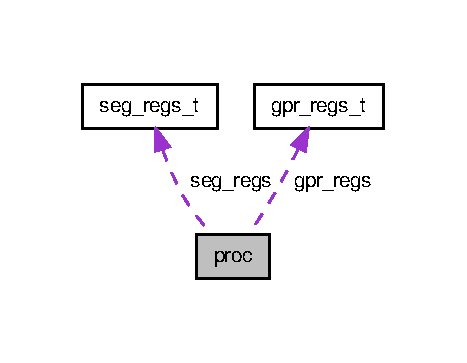
\includegraphics[width=224pt]{structproc__coll__graph}
\end{center}
\end{figure}
\subsection*{\-Public \-Member \-Functions}
\begin{DoxyCompactItemize}
\item 
\hyperlink{structproc_afa7308103cd5ed76c5d82dcdf7c44dd1}{\-L\-I\-S\-T\-\_\-\-E\-N\-T\-R\-Y} (\hyperlink{structproc}{proc}) link
\item 
\hyperlink{structproc_a47ec8cdb06b0ea0ae9d50289a37891b2}{\-L\-I\-F\-O\-\_\-\-E\-N\-T\-R\-Y} (\hyperlink{structproc}{proc}) q\-\_\-link
\end{DoxyCompactItemize}
\subsection*{\-Data \-Fields}
\begin{DoxyCompactItemize}
\item 
\hyperlink{structgpr__regs__t}{gpr\-\_\-regs\-\_\-t} \hyperlink{structproc_a477ac830839c6d6d6e7307e5b2e417d5}{gpr\-\_\-regs}
\item 
\hyperlink{structseg__regs__t}{seg\-\_\-regs\-\_\-t} \hyperlink{structproc_aee00499def5c013e7498cbe44b14cee1}{seg\-\_\-regs}
\item 
\hyperlink{types_8h_a089269ab3c13f602c75d4c7820175d67}{reg\-\_\-t} \hyperlink{structproc_a3df0fefa9b51a7e21c35c8c9fbc4f725}{eip}
\item 
\hyperlink{types_8h_a435d1572bf3f880d55459d9805097f62}{uint32\-\_\-t} \hyperlink{structproc_a5f1ddc555dad12aa7c3bb8137612da1a}{cs}
\item 
\hyperlink{types_8h_a089269ab3c13f602c75d4c7820175d67}{reg\-\_\-t} \hyperlink{structproc_a41e1d85590672d7aed7298c2553d1f6a}{eflags}
\item 
\hyperlink{types_8h_a089269ab3c13f602c75d4c7820175d67}{reg\-\_\-t} \hyperlink{structproc_aaeb0661f9e28aaad812437f33b0fea16}{esp}
\item 
\hyperlink{types_8h_a435d1572bf3f880d55459d9805097f62}{uint32\-\_\-t} \hyperlink{structproc_aa7c1976cb03e0295ef1dac2ddb52c900}{ss}
\item 
\hyperlink{types_8h_a435d1572bf3f880d55459d9805097f62}{uint32\-\_\-t} \hyperlink{structproc_a84a7b5847b08fe2a3f394d3cdacde847}{proc\-\_\-id}
\item 
\hyperlink{types_8h_a435d1572bf3f880d55459d9805097f62}{uint32\-\_\-t} \hyperlink{structproc_aac562ad34873ba0fe5766d6ab713ed03}{proc\-\_\-status}
\item 
\hyperlink{page_8h_a1ae9855ac82633447ab53f25e49e1f62}{pde\-\_\-t} $\ast$ \hyperlink{structproc_a28407ef578b1a5f1a5947400130516d5}{page\-\_\-directory}
\item 
\hyperlink{types_8h_a435d1572bf3f880d55459d9805097f62}{uint32\-\_\-t} \hyperlink{structproc_ab6ffe1dceb54452ad9f18ce2450aa8e9}{cr3}
\item 
\hyperlink{types_8h_a435d1572bf3f880d55459d9805097f62}{uint32\-\_\-t} \hyperlink{structproc_ac5ce1257f9f754b8d50b4aade713999d}{preempted}
\item 
\hyperlink{types_8h_a435d1572bf3f880d55459d9805097f62}{uint32\-\_\-t} \hyperlink{structproc_aa9f51aaaa65bdfe5220f65452b5b28d6}{dequeqed}
\end{DoxyCompactItemize}


\subsection{\-Detailed \-Description}


\-Definition at line 23 of file proc.\-h.



\subsection{\-Member \-Function \-Documentation}
\hypertarget{structproc_a47ec8cdb06b0ea0ae9d50289a37891b2}{\index{proc@{proc}!\-L\-I\-F\-O\-\_\-\-E\-N\-T\-R\-Y@{\-L\-I\-F\-O\-\_\-\-E\-N\-T\-R\-Y}}
\index{\-L\-I\-F\-O\-\_\-\-E\-N\-T\-R\-Y@{\-L\-I\-F\-O\-\_\-\-E\-N\-T\-R\-Y}!proc@{proc}}
\subsubsection[{\-L\-I\-F\-O\-\_\-\-E\-N\-T\-R\-Y}]{\setlength{\rightskip}{0pt plus 5cm}{\bf proc\-::\-L\-I\-F\-O\-\_\-\-E\-N\-T\-R\-Y} (
\begin{DoxyParamCaption}
\item[{{\bf proc}}]{}
\end{DoxyParamCaption}
)}}\label{structproc_a47ec8cdb06b0ea0ae9d50289a37891b2}
\hypertarget{structproc_afa7308103cd5ed76c5d82dcdf7c44dd1}{\index{proc@{proc}!\-L\-I\-S\-T\-\_\-\-E\-N\-T\-R\-Y@{\-L\-I\-S\-T\-\_\-\-E\-N\-T\-R\-Y}}
\index{\-L\-I\-S\-T\-\_\-\-E\-N\-T\-R\-Y@{\-L\-I\-S\-T\-\_\-\-E\-N\-T\-R\-Y}!proc@{proc}}
\subsubsection[{\-L\-I\-S\-T\-\_\-\-E\-N\-T\-R\-Y}]{\setlength{\rightskip}{0pt plus 5cm}{\bf proc\-::\-L\-I\-S\-T\-\_\-\-E\-N\-T\-R\-Y} (
\begin{DoxyParamCaption}
\item[{{\bf proc}}]{}
\end{DoxyParamCaption}
)}}\label{structproc_afa7308103cd5ed76c5d82dcdf7c44dd1}


\subsection{\-Field \-Documentation}
\hypertarget{structproc_ab6ffe1dceb54452ad9f18ce2450aa8e9}{\index{proc@{proc}!cr3@{cr3}}
\index{cr3@{cr3}!proc@{proc}}
\subsubsection[{cr3}]{\setlength{\rightskip}{0pt plus 5cm}{\bf uint32\-\_\-t} {\bf proc\-::cr3}}}\label{structproc_ab6ffe1dceb54452ad9f18ce2450aa8e9}


\-Definition at line 35 of file proc.\-h.

\hypertarget{structproc_a5f1ddc555dad12aa7c3bb8137612da1a}{\index{proc@{proc}!cs@{cs}}
\index{cs@{cs}!proc@{proc}}
\subsubsection[{cs}]{\setlength{\rightskip}{0pt plus 5cm}{\bf uint32\-\_\-t} {\bf proc\-::cs}}}\label{structproc_a5f1ddc555dad12aa7c3bb8137612da1a}


\-Definition at line 27 of file proc.\-h.

\hypertarget{structproc_aa9f51aaaa65bdfe5220f65452b5b28d6}{\index{proc@{proc}!dequeqed@{dequeqed}}
\index{dequeqed@{dequeqed}!proc@{proc}}
\subsubsection[{dequeqed}]{\setlength{\rightskip}{0pt plus 5cm}{\bf uint32\-\_\-t} {\bf proc\-::dequeqed}}}\label{structproc_aa9f51aaaa65bdfe5220f65452b5b28d6}


\-Definition at line 37 of file proc.\-h.

\hypertarget{structproc_a41e1d85590672d7aed7298c2553d1f6a}{\index{proc@{proc}!eflags@{eflags}}
\index{eflags@{eflags}!proc@{proc}}
\subsubsection[{eflags}]{\setlength{\rightskip}{0pt plus 5cm}{\bf reg\-\_\-t} {\bf proc\-::eflags}}}\label{structproc_a41e1d85590672d7aed7298c2553d1f6a}


\-Definition at line 28 of file proc.\-h.

\hypertarget{structproc_a3df0fefa9b51a7e21c35c8c9fbc4f725}{\index{proc@{proc}!eip@{eip}}
\index{eip@{eip}!proc@{proc}}
\subsubsection[{eip}]{\setlength{\rightskip}{0pt plus 5cm}{\bf reg\-\_\-t} {\bf proc\-::eip}}}\label{structproc_a3df0fefa9b51a7e21c35c8c9fbc4f725}


\-Definition at line 26 of file proc.\-h.

\hypertarget{structproc_aaeb0661f9e28aaad812437f33b0fea16}{\index{proc@{proc}!esp@{esp}}
\index{esp@{esp}!proc@{proc}}
\subsubsection[{esp}]{\setlength{\rightskip}{0pt plus 5cm}{\bf reg\-\_\-t} {\bf proc\-::esp}}}\label{structproc_aaeb0661f9e28aaad812437f33b0fea16}


\-Definition at line 29 of file proc.\-h.

\hypertarget{structproc_a477ac830839c6d6d6e7307e5b2e417d5}{\index{proc@{proc}!gpr\-\_\-regs@{gpr\-\_\-regs}}
\index{gpr\-\_\-regs@{gpr\-\_\-regs}!proc@{proc}}
\subsubsection[{gpr\-\_\-regs}]{\setlength{\rightskip}{0pt plus 5cm}{\bf gpr\-\_\-regs\-\_\-t} {\bf proc\-::gpr\-\_\-regs}}}\label{structproc_a477ac830839c6d6d6e7307e5b2e417d5}


\-Definition at line 24 of file proc.\-h.

\hypertarget{structproc_a28407ef578b1a5f1a5947400130516d5}{\index{proc@{proc}!page\-\_\-directory@{page\-\_\-directory}}
\index{page\-\_\-directory@{page\-\_\-directory}!proc@{proc}}
\subsubsection[{page\-\_\-directory}]{\setlength{\rightskip}{0pt plus 5cm}{\bf pde\-\_\-t}$\ast$ {\bf proc\-::page\-\_\-directory}}}\label{structproc_a28407ef578b1a5f1a5947400130516d5}


\-Definition at line 34 of file proc.\-h.

\hypertarget{structproc_ac5ce1257f9f754b8d50b4aade713999d}{\index{proc@{proc}!preempted@{preempted}}
\index{preempted@{preempted}!proc@{proc}}
\subsubsection[{preempted}]{\setlength{\rightskip}{0pt plus 5cm}{\bf uint32\-\_\-t} {\bf proc\-::preempted}}}\label{structproc_ac5ce1257f9f754b8d50b4aade713999d}


\-Definition at line 36 of file proc.\-h.

\hypertarget{structproc_a84a7b5847b08fe2a3f394d3cdacde847}{\index{proc@{proc}!proc\-\_\-id@{proc\-\_\-id}}
\index{proc\-\_\-id@{proc\-\_\-id}!proc@{proc}}
\subsubsection[{proc\-\_\-id}]{\setlength{\rightskip}{0pt plus 5cm}{\bf uint32\-\_\-t} {\bf proc\-::proc\-\_\-id}}}\label{structproc_a84a7b5847b08fe2a3f394d3cdacde847}


\-Definition at line 31 of file proc.\-h.

\hypertarget{structproc_aac562ad34873ba0fe5766d6ab713ed03}{\index{proc@{proc}!proc\-\_\-status@{proc\-\_\-status}}
\index{proc\-\_\-status@{proc\-\_\-status}!proc@{proc}}
\subsubsection[{proc\-\_\-status}]{\setlength{\rightskip}{0pt plus 5cm}{\bf uint32\-\_\-t} {\bf proc\-::proc\-\_\-status}}}\label{structproc_aac562ad34873ba0fe5766d6ab713ed03}


\-Definition at line 32 of file proc.\-h.

\hypertarget{structproc_aee00499def5c013e7498cbe44b14cee1}{\index{proc@{proc}!seg\-\_\-regs@{seg\-\_\-regs}}
\index{seg\-\_\-regs@{seg\-\_\-regs}!proc@{proc}}
\subsubsection[{seg\-\_\-regs}]{\setlength{\rightskip}{0pt plus 5cm}{\bf seg\-\_\-regs\-\_\-t} {\bf proc\-::seg\-\_\-regs}}}\label{structproc_aee00499def5c013e7498cbe44b14cee1}


\-Definition at line 25 of file proc.\-h.

\hypertarget{structproc_aa7c1976cb03e0295ef1dac2ddb52c900}{\index{proc@{proc}!ss@{ss}}
\index{ss@{ss}!proc@{proc}}
\subsubsection[{ss}]{\setlength{\rightskip}{0pt plus 5cm}{\bf uint32\-\_\-t} {\bf proc\-::ss}}}\label{structproc_aa7c1976cb03e0295ef1dac2ddb52c900}


\-Definition at line 30 of file proc.\-h.



\-The documentation for this struct was generated from the following file\-:\begin{DoxyCompactItemize}
\item 
include/proc/\hyperlink{proc_8h}{proc.\-h}\end{DoxyCompactItemize}

\hypertarget{structproghdr}{\section{proghdr \-Struct \-Reference}
\label{structproghdr}\index{proghdr@{proghdr}}
}


{\ttfamily \#include $<$elf.\-h$>$}

\subsection*{\-Data \-Fields}
\begin{DoxyCompactItemize}
\item 
\hyperlink{types_8h_a435d1572bf3f880d55459d9805097f62}{uint32\-\_\-t} \hyperlink{structproghdr_a523c83d0b884fb303b4b079e86a6aa55}{type}
\item 
\hyperlink{types_8h_a435d1572bf3f880d55459d9805097f62}{uint32\-\_\-t} \hyperlink{structproghdr_a13ca31beed71b97e906646eb21ab7c43}{offset}
\item 
\hyperlink{types_8h_a435d1572bf3f880d55459d9805097f62}{uint32\-\_\-t} \hyperlink{structproghdr_ac7edbebc9b5120c39b49301851765c42}{vaddr}
\item 
\hyperlink{types_8h_a435d1572bf3f880d55459d9805097f62}{uint32\-\_\-t} \hyperlink{structproghdr_aee40352ae868f605ca540d8d7c1ad71d}{paddr}
\item 
\hyperlink{types_8h_a435d1572bf3f880d55459d9805097f62}{uint32\-\_\-t} \hyperlink{structproghdr_ada45841c63724ee15300232b0317d1c3}{filesz}
\item 
\hyperlink{types_8h_a435d1572bf3f880d55459d9805097f62}{uint32\-\_\-t} \hyperlink{structproghdr_a1d2b052eeb75a24234f4fbb087205f71}{memsz}
\item 
\hyperlink{types_8h_a435d1572bf3f880d55459d9805097f62}{uint32\-\_\-t} \hyperlink{structproghdr_a5129c882410bcae83437e65617a9d0b3}{flags}
\item 
\hyperlink{types_8h_a435d1572bf3f880d55459d9805097f62}{uint32\-\_\-t} \hyperlink{structproghdr_a5912e1e2fba82b61114bdb12c50325a0}{align}
\end{DoxyCompactItemize}


\subsection{\-Detailed \-Description}


\-Definition at line 71 of file elf.\-h.



\subsection{\-Field \-Documentation}
\hypertarget{structproghdr_a5912e1e2fba82b61114bdb12c50325a0}{\index{proghdr@{proghdr}!align@{align}}
\index{align@{align}!proghdr@{proghdr}}
\subsubsection[{align}]{\setlength{\rightskip}{0pt plus 5cm}{\bf uint32\-\_\-t} {\bf proghdr\-::align}}}\label{structproghdr_a5912e1e2fba82b61114bdb12c50325a0}


\-Definition at line 79 of file elf.\-h.

\hypertarget{structproghdr_ada45841c63724ee15300232b0317d1c3}{\index{proghdr@{proghdr}!filesz@{filesz}}
\index{filesz@{filesz}!proghdr@{proghdr}}
\subsubsection[{filesz}]{\setlength{\rightskip}{0pt plus 5cm}{\bf uint32\-\_\-t} {\bf proghdr\-::filesz}}}\label{structproghdr_ada45841c63724ee15300232b0317d1c3}


\-Definition at line 76 of file elf.\-h.

\hypertarget{structproghdr_a5129c882410bcae83437e65617a9d0b3}{\index{proghdr@{proghdr}!flags@{flags}}
\index{flags@{flags}!proghdr@{proghdr}}
\subsubsection[{flags}]{\setlength{\rightskip}{0pt plus 5cm}{\bf uint32\-\_\-t} {\bf proghdr\-::flags}}}\label{structproghdr_a5129c882410bcae83437e65617a9d0b3}


\-Definition at line 78 of file elf.\-h.

\hypertarget{structproghdr_a1d2b052eeb75a24234f4fbb087205f71}{\index{proghdr@{proghdr}!memsz@{memsz}}
\index{memsz@{memsz}!proghdr@{proghdr}}
\subsubsection[{memsz}]{\setlength{\rightskip}{0pt plus 5cm}{\bf uint32\-\_\-t} {\bf proghdr\-::memsz}}}\label{structproghdr_a1d2b052eeb75a24234f4fbb087205f71}


\-Definition at line 77 of file elf.\-h.

\hypertarget{structproghdr_a13ca31beed71b97e906646eb21ab7c43}{\index{proghdr@{proghdr}!offset@{offset}}
\index{offset@{offset}!proghdr@{proghdr}}
\subsubsection[{offset}]{\setlength{\rightskip}{0pt plus 5cm}{\bf uint32\-\_\-t} {\bf proghdr\-::offset}}}\label{structproghdr_a13ca31beed71b97e906646eb21ab7c43}


\-Definition at line 73 of file elf.\-h.

\hypertarget{structproghdr_aee40352ae868f605ca540d8d7c1ad71d}{\index{proghdr@{proghdr}!paddr@{paddr}}
\index{paddr@{paddr}!proghdr@{proghdr}}
\subsubsection[{paddr}]{\setlength{\rightskip}{0pt plus 5cm}{\bf uint32\-\_\-t} {\bf proghdr\-::paddr}}}\label{structproghdr_aee40352ae868f605ca540d8d7c1ad71d}


\-Definition at line 75 of file elf.\-h.

\hypertarget{structproghdr_a523c83d0b884fb303b4b079e86a6aa55}{\index{proghdr@{proghdr}!type@{type}}
\index{type@{type}!proghdr@{proghdr}}
\subsubsection[{type}]{\setlength{\rightskip}{0pt plus 5cm}{\bf uint32\-\_\-t} {\bf proghdr\-::type}}}\label{structproghdr_a523c83d0b884fb303b4b079e86a6aa55}


\-Definition at line 72 of file elf.\-h.

\hypertarget{structproghdr_ac7edbebc9b5120c39b49301851765c42}{\index{proghdr@{proghdr}!vaddr@{vaddr}}
\index{vaddr@{vaddr}!proghdr@{proghdr}}
\subsubsection[{vaddr}]{\setlength{\rightskip}{0pt plus 5cm}{\bf uint32\-\_\-t} {\bf proghdr\-::vaddr}}}\label{structproghdr_ac7edbebc9b5120c39b49301851765c42}


\-Definition at line 74 of file elf.\-h.



\-The documentation for this struct was generated from the following file\-:\begin{DoxyCompactItemize}
\item 
include/arch/x86/\hyperlink{elf_8h}{elf.\-h}\end{DoxyCompactItemize}

\hypertarget{structsechdr}{\section{sechdr \-Struct \-Reference}
\label{structsechdr}\index{sechdr@{sechdr}}
}


{\ttfamily \#include $<$elf.\-h$>$}

\subsection*{\-Data \-Fields}
\begin{DoxyCompactItemize}
\item 
\hyperlink{types_8h_a435d1572bf3f880d55459d9805097f62}{uint32\-\_\-t} \hyperlink{structsechdr_a45bd257777c9fc7d036b6854755d8790}{name}
\item 
\hyperlink{types_8h_a435d1572bf3f880d55459d9805097f62}{uint32\-\_\-t} \hyperlink{structsechdr_acffd68b62e2e516fd537869d19041f01}{type}
\item 
\hyperlink{types_8h_a435d1572bf3f880d55459d9805097f62}{uint32\-\_\-t} \hyperlink{structsechdr_ad421a758659fa74ebff5f6ff3bca7a94}{flags}
\item 
\hyperlink{types_8h_a435d1572bf3f880d55459d9805097f62}{uint32\-\_\-t} \hyperlink{structsechdr_a01177bf70246483a03dd953d971e621d}{addr}
\item 
\hyperlink{types_8h_a435d1572bf3f880d55459d9805097f62}{uint32\-\_\-t} \hyperlink{structsechdr_aaae33ec54a7d3cb7e6c8138c4a716474}{offset}
\item 
\hyperlink{types_8h_a435d1572bf3f880d55459d9805097f62}{uint32\-\_\-t} \hyperlink{structsechdr_a309283bfb10685dfd97616963648fb96}{size}
\item 
\hyperlink{types_8h_a435d1572bf3f880d55459d9805097f62}{uint32\-\_\-t} \hyperlink{structsechdr_a23b277d435b5937eaad56740aa53a569}{link}
\item 
\hyperlink{types_8h_a435d1572bf3f880d55459d9805097f62}{uint32\-\_\-t} \hyperlink{structsechdr_ab42c2f90e8a62f87567a1b75836dcaa2}{info}
\item 
\hyperlink{types_8h_a435d1572bf3f880d55459d9805097f62}{uint32\-\_\-t} \hyperlink{structsechdr_acdef3f9bcf67524fb76a103170433b1f}{addralign}
\item 
\hyperlink{types_8h_a435d1572bf3f880d55459d9805097f62}{uint32\-\_\-t} \hyperlink{structsechdr_a68da29aef9f7b87f533b229abbaef452}{entsize}
\end{DoxyCompactItemize}


\subsection{\-Detailed \-Description}


\-Definition at line 82 of file elf.\-h.



\subsection{\-Field \-Documentation}
\hypertarget{structsechdr_a01177bf70246483a03dd953d971e621d}{\index{sechdr@{sechdr}!addr@{addr}}
\index{addr@{addr}!sechdr@{sechdr}}
\subsubsection[{addr}]{\setlength{\rightskip}{0pt plus 5cm}{\bf uint32\-\_\-t} {\bf sechdr\-::addr}}}\label{structsechdr_a01177bf70246483a03dd953d971e621d}


\-Definition at line 86 of file elf.\-h.

\hypertarget{structsechdr_acdef3f9bcf67524fb76a103170433b1f}{\index{sechdr@{sechdr}!addralign@{addralign}}
\index{addralign@{addralign}!sechdr@{sechdr}}
\subsubsection[{addralign}]{\setlength{\rightskip}{0pt plus 5cm}{\bf uint32\-\_\-t} {\bf sechdr\-::addralign}}}\label{structsechdr_acdef3f9bcf67524fb76a103170433b1f}


\-Definition at line 91 of file elf.\-h.

\hypertarget{structsechdr_a68da29aef9f7b87f533b229abbaef452}{\index{sechdr@{sechdr}!entsize@{entsize}}
\index{entsize@{entsize}!sechdr@{sechdr}}
\subsubsection[{entsize}]{\setlength{\rightskip}{0pt plus 5cm}{\bf uint32\-\_\-t} {\bf sechdr\-::entsize}}}\label{structsechdr_a68da29aef9f7b87f533b229abbaef452}


\-Definition at line 92 of file elf.\-h.

\hypertarget{structsechdr_ad421a758659fa74ebff5f6ff3bca7a94}{\index{sechdr@{sechdr}!flags@{flags}}
\index{flags@{flags}!sechdr@{sechdr}}
\subsubsection[{flags}]{\setlength{\rightskip}{0pt plus 5cm}{\bf uint32\-\_\-t} {\bf sechdr\-::flags}}}\label{structsechdr_ad421a758659fa74ebff5f6ff3bca7a94}


\-Definition at line 85 of file elf.\-h.

\hypertarget{structsechdr_ab42c2f90e8a62f87567a1b75836dcaa2}{\index{sechdr@{sechdr}!info@{info}}
\index{info@{info}!sechdr@{sechdr}}
\subsubsection[{info}]{\setlength{\rightskip}{0pt plus 5cm}{\bf uint32\-\_\-t} {\bf sechdr\-::info}}}\label{structsechdr_ab42c2f90e8a62f87567a1b75836dcaa2}


\-Definition at line 90 of file elf.\-h.

\hypertarget{structsechdr_a23b277d435b5937eaad56740aa53a569}{\index{sechdr@{sechdr}!link@{link}}
\index{link@{link}!sechdr@{sechdr}}
\subsubsection[{link}]{\setlength{\rightskip}{0pt plus 5cm}{\bf uint32\-\_\-t} {\bf sechdr\-::link}}}\label{structsechdr_a23b277d435b5937eaad56740aa53a569}


\-Definition at line 89 of file elf.\-h.

\hypertarget{structsechdr_a45bd257777c9fc7d036b6854755d8790}{\index{sechdr@{sechdr}!name@{name}}
\index{name@{name}!sechdr@{sechdr}}
\subsubsection[{name}]{\setlength{\rightskip}{0pt plus 5cm}{\bf uint32\-\_\-t} {\bf sechdr\-::name}}}\label{structsechdr_a45bd257777c9fc7d036b6854755d8790}


\-Definition at line 83 of file elf.\-h.

\hypertarget{structsechdr_aaae33ec54a7d3cb7e6c8138c4a716474}{\index{sechdr@{sechdr}!offset@{offset}}
\index{offset@{offset}!sechdr@{sechdr}}
\subsubsection[{offset}]{\setlength{\rightskip}{0pt plus 5cm}{\bf uint32\-\_\-t} {\bf sechdr\-::offset}}}\label{structsechdr_aaae33ec54a7d3cb7e6c8138c4a716474}


\-Definition at line 87 of file elf.\-h.

\hypertarget{structsechdr_a309283bfb10685dfd97616963648fb96}{\index{sechdr@{sechdr}!size@{size}}
\index{size@{size}!sechdr@{sechdr}}
\subsubsection[{size}]{\setlength{\rightskip}{0pt plus 5cm}{\bf uint32\-\_\-t} {\bf sechdr\-::size}}}\label{structsechdr_a309283bfb10685dfd97616963648fb96}


\-Definition at line 88 of file elf.\-h.

\hypertarget{structsechdr_acffd68b62e2e516fd537869d19041f01}{\index{sechdr@{sechdr}!type@{type}}
\index{type@{type}!sechdr@{sechdr}}
\subsubsection[{type}]{\setlength{\rightskip}{0pt plus 5cm}{\bf uint32\-\_\-t} {\bf sechdr\-::type}}}\label{structsechdr_acffd68b62e2e516fd537869d19041f01}


\-Definition at line 84 of file elf.\-h.



\-The documentation for this struct was generated from the following file\-:\begin{DoxyCompactItemize}
\item 
include/arch/x86/\hyperlink{elf_8h}{elf.\-h}\end{DoxyCompactItemize}

\hypertarget{structseg__regs__t}{\section{seg\-\_\-regs\-\_\-t \-Struct \-Reference}
\label{structseg__regs__t}\index{seg\-\_\-regs\-\_\-t@{seg\-\_\-regs\-\_\-t}}
}


{\ttfamily \#include $<$cpu\-\_\-state.\-h$>$}

\subsection*{\-Data \-Fields}
\begin{DoxyCompactItemize}
\item 
\hyperlink{types_8h_a089269ab3c13f602c75d4c7820175d67}{reg\-\_\-t} \hyperlink{structseg__regs__t_af3c39996499f1c4885ce96121f2fdde7}{gs}
\item 
\hyperlink{types_8h_a089269ab3c13f602c75d4c7820175d67}{reg\-\_\-t} \hyperlink{structseg__regs__t_a49bcd2ca05a6613d1ed6ff1c1b062940}{fs}
\item 
\hyperlink{types_8h_a089269ab3c13f602c75d4c7820175d67}{reg\-\_\-t} \hyperlink{structseg__regs__t_a2cba36244f3431cf78336175e73e9244}{es}
\item 
\hyperlink{types_8h_a089269ab3c13f602c75d4c7820175d67}{reg\-\_\-t} \hyperlink{structseg__regs__t_ade33634359bc73e66892961923388104}{ds}
\end{DoxyCompactItemize}


\subsection{\-Detailed \-Description}


\-Definition at line 80 of file cpu\-\_\-state.\-h.



\subsection{\-Field \-Documentation}
\hypertarget{structseg__regs__t_ade33634359bc73e66892961923388104}{\index{seg\-\_\-regs\-\_\-t@{seg\-\_\-regs\-\_\-t}!ds@{ds}}
\index{ds@{ds}!seg_regs_t@{seg\-\_\-regs\-\_\-t}}
\subsubsection[{ds}]{\setlength{\rightskip}{0pt plus 5cm}{\bf reg\-\_\-t} {\bf seg\-\_\-regs\-\_\-t\-::ds}}}\label{structseg__regs__t_ade33634359bc73e66892961923388104}


\-Definition at line 84 of file cpu\-\_\-state.\-h.

\hypertarget{structseg__regs__t_a2cba36244f3431cf78336175e73e9244}{\index{seg\-\_\-regs\-\_\-t@{seg\-\_\-regs\-\_\-t}!es@{es}}
\index{es@{es}!seg_regs_t@{seg\-\_\-regs\-\_\-t}}
\subsubsection[{es}]{\setlength{\rightskip}{0pt plus 5cm}{\bf reg\-\_\-t} {\bf seg\-\_\-regs\-\_\-t\-::es}}}\label{structseg__regs__t_a2cba36244f3431cf78336175e73e9244}


\-Definition at line 83 of file cpu\-\_\-state.\-h.

\hypertarget{structseg__regs__t_a49bcd2ca05a6613d1ed6ff1c1b062940}{\index{seg\-\_\-regs\-\_\-t@{seg\-\_\-regs\-\_\-t}!fs@{fs}}
\index{fs@{fs}!seg_regs_t@{seg\-\_\-regs\-\_\-t}}
\subsubsection[{fs}]{\setlength{\rightskip}{0pt plus 5cm}{\bf reg\-\_\-t} {\bf seg\-\_\-regs\-\_\-t\-::fs}}}\label{structseg__regs__t_a49bcd2ca05a6613d1ed6ff1c1b062940}


\-Definition at line 82 of file cpu\-\_\-state.\-h.

\hypertarget{structseg__regs__t_af3c39996499f1c4885ce96121f2fdde7}{\index{seg\-\_\-regs\-\_\-t@{seg\-\_\-regs\-\_\-t}!gs@{gs}}
\index{gs@{gs}!seg_regs_t@{seg\-\_\-regs\-\_\-t}}
\subsubsection[{gs}]{\setlength{\rightskip}{0pt plus 5cm}{\bf reg\-\_\-t} {\bf seg\-\_\-regs\-\_\-t\-::gs}}}\label{structseg__regs__t_af3c39996499f1c4885ce96121f2fdde7}


\-Definition at line 81 of file cpu\-\_\-state.\-h.



\-The documentation for this struct was generated from the following file\-:\begin{DoxyCompactItemize}
\item 
include/arch/x86/\hyperlink{cpu__state_8h}{cpu\-\_\-state.\-h}\end{DoxyCompactItemize}

\hypertarget{structSegdesc}{\section{\-Segdesc \-Struct \-Reference}
\label{structSegdesc}\index{\-Segdesc@{\-Segdesc}}
}


{\ttfamily \#include $<$memvals.\-h$>$}

\subsection*{\-Data \-Fields}
\begin{DoxyCompactItemize}
\item 
unsigned \hyperlink{structSegdesc_aa98356a03ede9a64a2a866c63d751b10}{limit\-\_\-0}\-: 16
\item 
unsigned \hyperlink{structSegdesc_a9ef72e5343428076ae56aadda868e6d6}{base\-\_\-0}\-: 16
\item 
unsigned \hyperlink{structSegdesc_a293c20d519e6ab9e38720e32016f7d31}{base\-\_\-1}\-: 8
\item 
unsigned \hyperlink{structSegdesc_a2ab463dbb1b304bf3ab79ba0abaf4eaa}{permission}\-: 8
\item 
unsigned \hyperlink{structSegdesc_a6ea96b5b37b07766d86d62c166363c21}{limit\-\_\-1}\-: 4
\item 
unsigned \hyperlink{structSegdesc_a88cc0fd4e0fc4467546577095c0ffe3e}{flags}\-: 4
\item 
unsigned \hyperlink{structSegdesc_a9f663ff44e5b7c7bffd2b5b72654d72e}{base}\-: 8
\end{DoxyCompactItemize}


\subsection{\-Detailed \-Description}


\-Definition at line 34 of file memvals.\-h.



\subsection{\-Field \-Documentation}
\hypertarget{structSegdesc_a9f663ff44e5b7c7bffd2b5b72654d72e}{\index{\-Segdesc@{\-Segdesc}!base@{base}}
\index{base@{base}!Segdesc@{\-Segdesc}}
\subsubsection[{base}]{\setlength{\rightskip}{0pt plus 5cm}unsigned {\bf \-Segdesc\-::base}}}\label{structSegdesc_a9f663ff44e5b7c7bffd2b5b72654d72e}


\-Definition at line 41 of file memvals.\-h.

\hypertarget{structSegdesc_a9ef72e5343428076ae56aadda868e6d6}{\index{\-Segdesc@{\-Segdesc}!base\-\_\-0@{base\-\_\-0}}
\index{base\-\_\-0@{base\-\_\-0}!Segdesc@{\-Segdesc}}
\subsubsection[{base\-\_\-0}]{\setlength{\rightskip}{0pt plus 5cm}unsigned {\bf \-Segdesc\-::base\-\_\-0}}}\label{structSegdesc_a9ef72e5343428076ae56aadda868e6d6}


\-Definition at line 36 of file memvals.\-h.

\hypertarget{structSegdesc_a293c20d519e6ab9e38720e32016f7d31}{\index{\-Segdesc@{\-Segdesc}!base\-\_\-1@{base\-\_\-1}}
\index{base\-\_\-1@{base\-\_\-1}!Segdesc@{\-Segdesc}}
\subsubsection[{base\-\_\-1}]{\setlength{\rightskip}{0pt plus 5cm}unsigned {\bf \-Segdesc\-::base\-\_\-1}}}\label{structSegdesc_a293c20d519e6ab9e38720e32016f7d31}


\-Definition at line 37 of file memvals.\-h.

\hypertarget{structSegdesc_a88cc0fd4e0fc4467546577095c0ffe3e}{\index{\-Segdesc@{\-Segdesc}!flags@{flags}}
\index{flags@{flags}!Segdesc@{\-Segdesc}}
\subsubsection[{flags}]{\setlength{\rightskip}{0pt plus 5cm}unsigned {\bf \-Segdesc\-::flags}}}\label{structSegdesc_a88cc0fd4e0fc4467546577095c0ffe3e}


\-Definition at line 40 of file memvals.\-h.

\hypertarget{structSegdesc_aa98356a03ede9a64a2a866c63d751b10}{\index{\-Segdesc@{\-Segdesc}!limit\-\_\-0@{limit\-\_\-0}}
\index{limit\-\_\-0@{limit\-\_\-0}!Segdesc@{\-Segdesc}}
\subsubsection[{limit\-\_\-0}]{\setlength{\rightskip}{0pt plus 5cm}unsigned {\bf \-Segdesc\-::limit\-\_\-0}}}\label{structSegdesc_aa98356a03ede9a64a2a866c63d751b10}


\-Definition at line 35 of file memvals.\-h.

\hypertarget{structSegdesc_a6ea96b5b37b07766d86d62c166363c21}{\index{\-Segdesc@{\-Segdesc}!limit\-\_\-1@{limit\-\_\-1}}
\index{limit\-\_\-1@{limit\-\_\-1}!Segdesc@{\-Segdesc}}
\subsubsection[{limit\-\_\-1}]{\setlength{\rightskip}{0pt plus 5cm}unsigned {\bf \-Segdesc\-::limit\-\_\-1}}}\label{structSegdesc_a6ea96b5b37b07766d86d62c166363c21}


\-Definition at line 39 of file memvals.\-h.

\hypertarget{structSegdesc_a2ab463dbb1b304bf3ab79ba0abaf4eaa}{\index{\-Segdesc@{\-Segdesc}!permission@{permission}}
\index{permission@{permission}!Segdesc@{\-Segdesc}}
\subsubsection[{permission}]{\setlength{\rightskip}{0pt plus 5cm}unsigned {\bf \-Segdesc\-::permission}}}\label{structSegdesc_a2ab463dbb1b304bf3ab79ba0abaf4eaa}


\-Definition at line 38 of file memvals.\-h.



\-The documentation for this struct was generated from the following file\-:\begin{DoxyCompactItemize}
\item 
include/\hyperlink{memvals_8h}{memvals.\-h}\end{DoxyCompactItemize}

\chapter{\-File \-Documentation}
\hypertarget{cpu__state_8h}{\section{include/arch/x86/cpu\-\_\-state.h \-File \-Reference}
\label{cpu__state_8h}\index{include/arch/x86/cpu\-\_\-state.\-h@{include/arch/x86/cpu\-\_\-state.\-h}}
}
{\ttfamily \#include $<$types.\-h$>$}\*
\-Include dependency graph for cpu\-\_\-state.\-h\-:\nopagebreak
\begin{figure}[H]
\begin{center}
\leavevmode
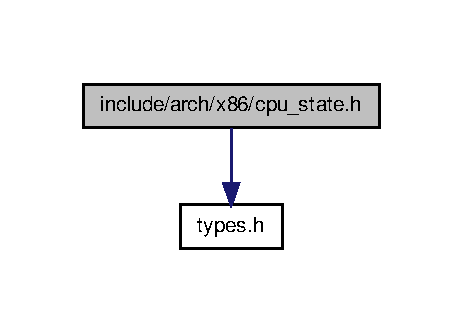
\includegraphics[width=222pt]{cpu__state_8h__incl}
\end{center}
\end{figure}
\-This graph shows which files directly or indirectly include this file\-:\nopagebreak
\begin{figure}[H]
\begin{center}
\leavevmode
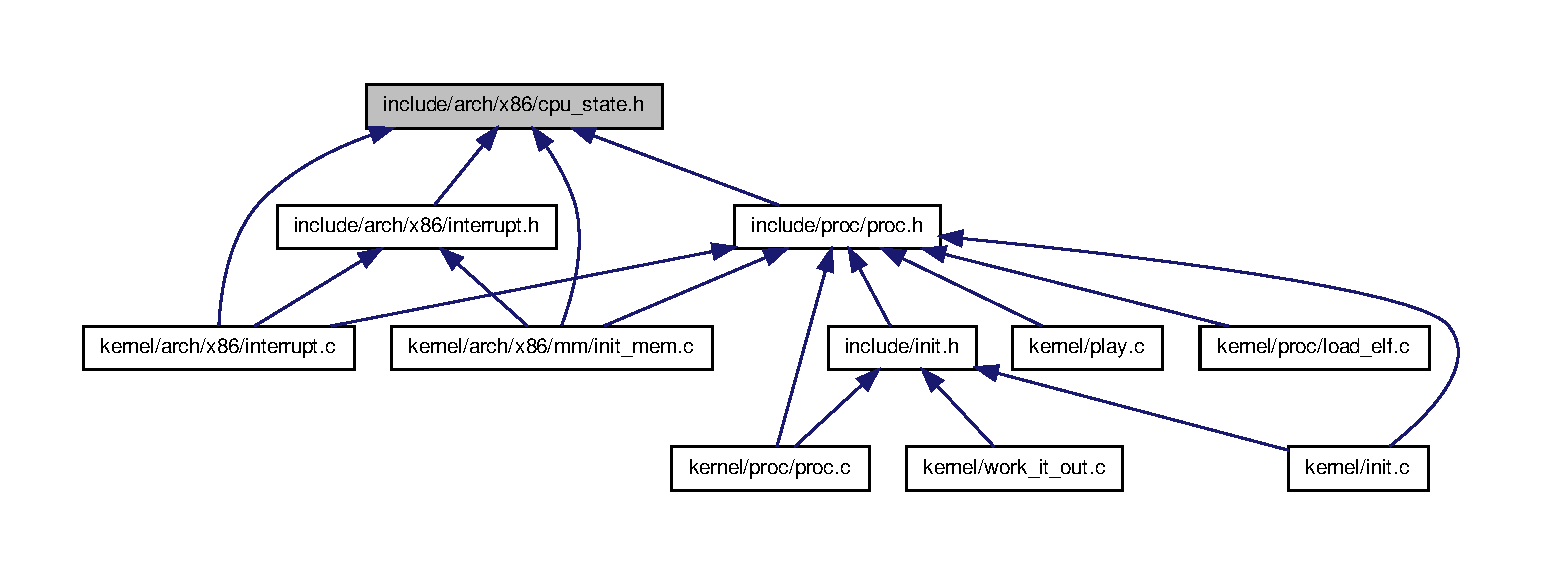
\includegraphics[width=350pt]{cpu__state_8h__dep__incl}
\end{center}
\end{figure}
\subsection*{\-Data \-Structures}
\begin{DoxyCompactItemize}
\item 
struct \hyperlink{structcpu__state__t}{cpu\-\_\-state\-\_\-t}
\item 
struct \hyperlink{structgpr__regs__t}{gpr\-\_\-regs\-\_\-t}
\item 
struct \hyperlink{structseg__regs__t}{seg\-\_\-regs\-\_\-t}
\item 
struct \hyperlink{struct____attribute____}{\-\_\-\-\_\-attribute\-\_\-\-\_\-}
\item 
struct \hyperlink{struct____attribute____}{\-\_\-\-\_\-attribute\-\_\-\-\_\-}
\end{DoxyCompactItemize}
\subsection*{\-Defines}
\begin{DoxyCompactItemize}
\item 
\#define \hyperlink{cpu__state_8h_a897f1c9251d78409c0c087a3aa6a9751}{\-T\-S\-S\-\_\-\-S\-I\-Z\-E}~104
\item 
\#define \hyperlink{cpu__state_8h_a14d167f362c5f12f1e1df058ab8e8525}{\-T\-S\-S\-\_\-\-I\-O\-M\-A\-P\-\_\-\-S\-I\-Z\-E}~((0x8 $\ast$ 0x400) +1)
\item 
\#define \hyperlink{cpu__state_8h_a9da172d7926a4ac6750a88ec25a4ed66}{\-T\-A\-S\-K\-\_\-\-B\-U\-S\-Y}~0x\-B
\item 
\#define \hyperlink{cpu__state_8h_a825f76f738df400cd95e221f5d58c2f2}{\-T\-A\-S\-K\-\_\-\-I\-N\-A\-C\-T\-I\-V\-E}~0x9
\item 
\#define \hyperlink{cpu__state_8h_a1c355106405ba3abfafe2e14e895e326}{\-T\-S\-S\-\_\-\-A\-V\-L}~1
\item 
\#define \hyperlink{cpu__state_8h_ac6ff4f02a79c5c4f7ed29a1b07ce9248}{\-T\-S\-S\-\_\-\-D\-P\-L\-\_\-\-K\-E\-R\-N\-E\-L}~0
\item 
\#define \hyperlink{cpu__state_8h_ace2adafa9b4fde415be899de1be3eb0a}{\-T\-S\-S\-\_\-\-D\-P\-L\-\_\-\-U\-S\-E\-R}~60
\item 
\#define \hyperlink{cpu__state_8h_a4cd0fdcefb1cae7c52486dc2f4158130}{\-T\-S\-S\-\_\-\-P\-R\-E\-S\-E\-N\-T}~0x80
\item 
\#define \hyperlink{cpu__state_8h_a82f227e201b9ed566b11299afe0d73b0}{\-T\-S\-S\-\_\-\-G\-R\-A\-N\-U\-L\-A\-R\-I\-T\-Y}~0x8
\item 
\#define \hyperlink{cpu__state_8h_a5127ef2278434881fdce2f6502cba29b}{\-S\-E\-G\-M\-E\-N\-T\-\_\-\-T\-S\-S}(limit, \hyperlink{memvals_8h_a0523cedff47e2441fc198b7770ec5d3f}{base}, type, flags)
\end{DoxyCompactItemize}


\subsection{\-Define \-Documentation}
\hypertarget{cpu__state_8h_a5127ef2278434881fdce2f6502cba29b}{\index{cpu\-\_\-state.\-h@{cpu\-\_\-state.\-h}!\-S\-E\-G\-M\-E\-N\-T\-\_\-\-T\-S\-S@{\-S\-E\-G\-M\-E\-N\-T\-\_\-\-T\-S\-S}}
\index{\-S\-E\-G\-M\-E\-N\-T\-\_\-\-T\-S\-S@{\-S\-E\-G\-M\-E\-N\-T\-\_\-\-T\-S\-S}!cpu_state.h@{cpu\-\_\-state.\-h}}
\subsubsection[{\-S\-E\-G\-M\-E\-N\-T\-\_\-\-T\-S\-S}]{\setlength{\rightskip}{0pt plus 5cm}\#define {\bf \-S\-E\-G\-M\-E\-N\-T\-\_\-\-T\-S\-S}(
\begin{DoxyParamCaption}
\item[{}]{limit, }
\item[{}]{{\bf base}, }
\item[{}]{type, }
\item[{}]{flags}
\end{DoxyParamCaption}
)}}\label{cpu__state_8h_a5127ef2278434881fdce2f6502cba29b}
{\bfseries \-Value\-:}
\begin{DoxyCode}
(struct Segdesc)\
        {       \
        (((limit)>>12) & 0xffff),       \
        ((base) & 0xffff),      \
        (((base) >> 16) & 0xff),        \
        (type), \
        ((limit) >> 28),        \
        ((flags)),      \
        (((base) >> 24) & 0xff) \
        }
\end{DoxyCode}


\-Definition at line 144 of file cpu\-\_\-state.\-h.

\hypertarget{cpu__state_8h_a9da172d7926a4ac6750a88ec25a4ed66}{\index{cpu\-\_\-state.\-h@{cpu\-\_\-state.\-h}!\-T\-A\-S\-K\-\_\-\-B\-U\-S\-Y@{\-T\-A\-S\-K\-\_\-\-B\-U\-S\-Y}}
\index{\-T\-A\-S\-K\-\_\-\-B\-U\-S\-Y@{\-T\-A\-S\-K\-\_\-\-B\-U\-S\-Y}!cpu_state.h@{cpu\-\_\-state.\-h}}
\subsubsection[{\-T\-A\-S\-K\-\_\-\-B\-U\-S\-Y}]{\setlength{\rightskip}{0pt plus 5cm}\#define {\bf \-T\-A\-S\-K\-\_\-\-B\-U\-S\-Y}~0x\-B}}\label{cpu__state_8h_a9da172d7926a4ac6750a88ec25a4ed66}


\-Definition at line 136 of file cpu\-\_\-state.\-h.

\hypertarget{cpu__state_8h_a825f76f738df400cd95e221f5d58c2f2}{\index{cpu\-\_\-state.\-h@{cpu\-\_\-state.\-h}!\-T\-A\-S\-K\-\_\-\-I\-N\-A\-C\-T\-I\-V\-E@{\-T\-A\-S\-K\-\_\-\-I\-N\-A\-C\-T\-I\-V\-E}}
\index{\-T\-A\-S\-K\-\_\-\-I\-N\-A\-C\-T\-I\-V\-E@{\-T\-A\-S\-K\-\_\-\-I\-N\-A\-C\-T\-I\-V\-E}!cpu_state.h@{cpu\-\_\-state.\-h}}
\subsubsection[{\-T\-A\-S\-K\-\_\-\-I\-N\-A\-C\-T\-I\-V\-E}]{\setlength{\rightskip}{0pt plus 5cm}\#define {\bf \-T\-A\-S\-K\-\_\-\-I\-N\-A\-C\-T\-I\-V\-E}~0x9}}\label{cpu__state_8h_a825f76f738df400cd95e221f5d58c2f2}


\-Definition at line 137 of file cpu\-\_\-state.\-h.

\hypertarget{cpu__state_8h_a1c355106405ba3abfafe2e14e895e326}{\index{cpu\-\_\-state.\-h@{cpu\-\_\-state.\-h}!\-T\-S\-S\-\_\-\-A\-V\-L@{\-T\-S\-S\-\_\-\-A\-V\-L}}
\index{\-T\-S\-S\-\_\-\-A\-V\-L@{\-T\-S\-S\-\_\-\-A\-V\-L}!cpu_state.h@{cpu\-\_\-state.\-h}}
\subsubsection[{\-T\-S\-S\-\_\-\-A\-V\-L}]{\setlength{\rightskip}{0pt plus 5cm}\#define {\bf \-T\-S\-S\-\_\-\-A\-V\-L}~1}}\label{cpu__state_8h_a1c355106405ba3abfafe2e14e895e326}


\-Definition at line 138 of file cpu\-\_\-state.\-h.

\hypertarget{cpu__state_8h_ac6ff4f02a79c5c4f7ed29a1b07ce9248}{\index{cpu\-\_\-state.\-h@{cpu\-\_\-state.\-h}!\-T\-S\-S\-\_\-\-D\-P\-L\-\_\-\-K\-E\-R\-N\-E\-L@{\-T\-S\-S\-\_\-\-D\-P\-L\-\_\-\-K\-E\-R\-N\-E\-L}}
\index{\-T\-S\-S\-\_\-\-D\-P\-L\-\_\-\-K\-E\-R\-N\-E\-L@{\-T\-S\-S\-\_\-\-D\-P\-L\-\_\-\-K\-E\-R\-N\-E\-L}!cpu_state.h@{cpu\-\_\-state.\-h}}
\subsubsection[{\-T\-S\-S\-\_\-\-D\-P\-L\-\_\-\-K\-E\-R\-N\-E\-L}]{\setlength{\rightskip}{0pt plus 5cm}\#define {\bf \-T\-S\-S\-\_\-\-D\-P\-L\-\_\-\-K\-E\-R\-N\-E\-L}~0}}\label{cpu__state_8h_ac6ff4f02a79c5c4f7ed29a1b07ce9248}


\-Definition at line 139 of file cpu\-\_\-state.\-h.

\hypertarget{cpu__state_8h_ace2adafa9b4fde415be899de1be3eb0a}{\index{cpu\-\_\-state.\-h@{cpu\-\_\-state.\-h}!\-T\-S\-S\-\_\-\-D\-P\-L\-\_\-\-U\-S\-E\-R@{\-T\-S\-S\-\_\-\-D\-P\-L\-\_\-\-U\-S\-E\-R}}
\index{\-T\-S\-S\-\_\-\-D\-P\-L\-\_\-\-U\-S\-E\-R@{\-T\-S\-S\-\_\-\-D\-P\-L\-\_\-\-U\-S\-E\-R}!cpu_state.h@{cpu\-\_\-state.\-h}}
\subsubsection[{\-T\-S\-S\-\_\-\-D\-P\-L\-\_\-\-U\-S\-E\-R}]{\setlength{\rightskip}{0pt plus 5cm}\#define {\bf \-T\-S\-S\-\_\-\-D\-P\-L\-\_\-\-U\-S\-E\-R}~60}}\label{cpu__state_8h_ace2adafa9b4fde415be899de1be3eb0a}


\-Definition at line 140 of file cpu\-\_\-state.\-h.

\hypertarget{cpu__state_8h_a82f227e201b9ed566b11299afe0d73b0}{\index{cpu\-\_\-state.\-h@{cpu\-\_\-state.\-h}!\-T\-S\-S\-\_\-\-G\-R\-A\-N\-U\-L\-A\-R\-I\-T\-Y@{\-T\-S\-S\-\_\-\-G\-R\-A\-N\-U\-L\-A\-R\-I\-T\-Y}}
\index{\-T\-S\-S\-\_\-\-G\-R\-A\-N\-U\-L\-A\-R\-I\-T\-Y@{\-T\-S\-S\-\_\-\-G\-R\-A\-N\-U\-L\-A\-R\-I\-T\-Y}!cpu_state.h@{cpu\-\_\-state.\-h}}
\subsubsection[{\-T\-S\-S\-\_\-\-G\-R\-A\-N\-U\-L\-A\-R\-I\-T\-Y}]{\setlength{\rightskip}{0pt plus 5cm}\#define {\bf \-T\-S\-S\-\_\-\-G\-R\-A\-N\-U\-L\-A\-R\-I\-T\-Y}~0x8}}\label{cpu__state_8h_a82f227e201b9ed566b11299afe0d73b0}


\-Definition at line 142 of file cpu\-\_\-state.\-h.

\hypertarget{cpu__state_8h_a14d167f362c5f12f1e1df058ab8e8525}{\index{cpu\-\_\-state.\-h@{cpu\-\_\-state.\-h}!\-T\-S\-S\-\_\-\-I\-O\-M\-A\-P\-\_\-\-S\-I\-Z\-E@{\-T\-S\-S\-\_\-\-I\-O\-M\-A\-P\-\_\-\-S\-I\-Z\-E}}
\index{\-T\-S\-S\-\_\-\-I\-O\-M\-A\-P\-\_\-\-S\-I\-Z\-E@{\-T\-S\-S\-\_\-\-I\-O\-M\-A\-P\-\_\-\-S\-I\-Z\-E}!cpu_state.h@{cpu\-\_\-state.\-h}}
\subsubsection[{\-T\-S\-S\-\_\-\-I\-O\-M\-A\-P\-\_\-\-S\-I\-Z\-E}]{\setlength{\rightskip}{0pt plus 5cm}\#define {\bf \-T\-S\-S\-\_\-\-I\-O\-M\-A\-P\-\_\-\-S\-I\-Z\-E}~((0x8 $\ast$ 0x400) +1)}}\label{cpu__state_8h_a14d167f362c5f12f1e1df058ab8e8525}


\-Definition at line 135 of file cpu\-\_\-state.\-h.

\hypertarget{cpu__state_8h_a4cd0fdcefb1cae7c52486dc2f4158130}{\index{cpu\-\_\-state.\-h@{cpu\-\_\-state.\-h}!\-T\-S\-S\-\_\-\-P\-R\-E\-S\-E\-N\-T@{\-T\-S\-S\-\_\-\-P\-R\-E\-S\-E\-N\-T}}
\index{\-T\-S\-S\-\_\-\-P\-R\-E\-S\-E\-N\-T@{\-T\-S\-S\-\_\-\-P\-R\-E\-S\-E\-N\-T}!cpu_state.h@{cpu\-\_\-state.\-h}}
\subsubsection[{\-T\-S\-S\-\_\-\-P\-R\-E\-S\-E\-N\-T}]{\setlength{\rightskip}{0pt plus 5cm}\#define {\bf \-T\-S\-S\-\_\-\-P\-R\-E\-S\-E\-N\-T}~0x80}}\label{cpu__state_8h_a4cd0fdcefb1cae7c52486dc2f4158130}


\-Definition at line 141 of file cpu\-\_\-state.\-h.

\hypertarget{cpu__state_8h_a897f1c9251d78409c0c087a3aa6a9751}{\index{cpu\-\_\-state.\-h@{cpu\-\_\-state.\-h}!\-T\-S\-S\-\_\-\-S\-I\-Z\-E@{\-T\-S\-S\-\_\-\-S\-I\-Z\-E}}
\index{\-T\-S\-S\-\_\-\-S\-I\-Z\-E@{\-T\-S\-S\-\_\-\-S\-I\-Z\-E}!cpu_state.h@{cpu\-\_\-state.\-h}}
\subsubsection[{\-T\-S\-S\-\_\-\-S\-I\-Z\-E}]{\setlength{\rightskip}{0pt plus 5cm}\#define {\bf \-T\-S\-S\-\_\-\-S\-I\-Z\-E}~104}}\label{cpu__state_8h_a897f1c9251d78409c0c087a3aa6a9751}


\-Definition at line 134 of file cpu\-\_\-state.\-h.


\hypertarget{elf_8h}{\section{include/arch/x86/elf.h \-File \-Reference}
\label{elf_8h}\index{include/arch/x86/elf.\-h@{include/arch/x86/elf.\-h}}
}
\-This graph shows which files directly or indirectly include this file\-:\nopagebreak
\begin{figure}[H]
\begin{center}
\leavevmode
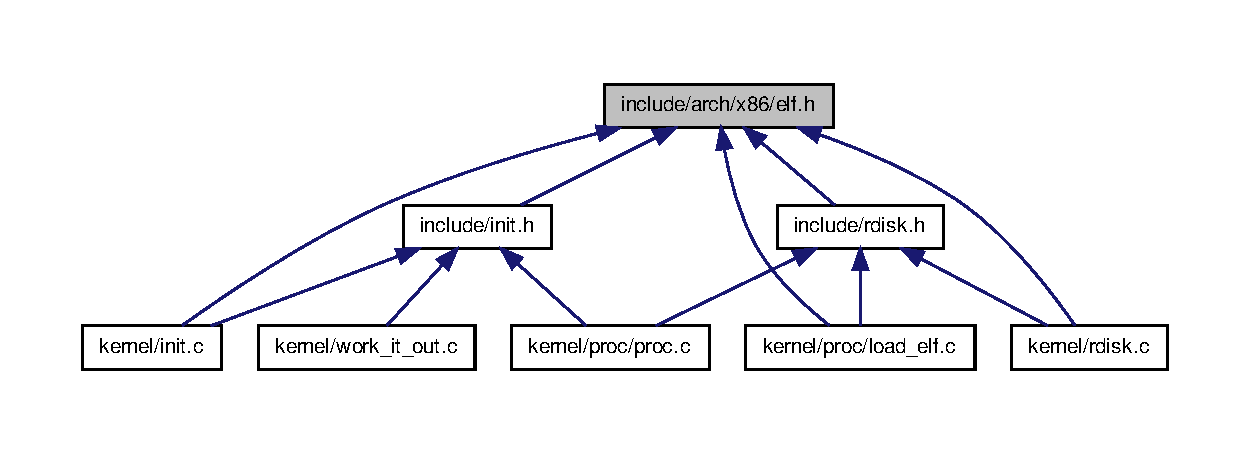
\includegraphics[width=350pt]{elf_8h__dep__incl}
\end{center}
\end{figure}
\subsection*{\-Data \-Structures}
\begin{DoxyCompactItemize}
\item 
struct \hyperlink{structelfhdr}{elfhdr}
\item 
struct \hyperlink{structproghdr}{proghdr}
\item 
struct \hyperlink{structsechdr}{sechdr}
\end{DoxyCompactItemize}
\subsection*{\-Defines}
\begin{DoxyCompactItemize}
\item 
\#define \hyperlink{elf_8h_abb1c2e5626667aacc7b3efd269a6c0eb}{\-E\-L\-F\-\_\-\-M\-A\-G\-I\-C}~0x464\-C457\-F
\item 
\#define \hyperlink{elf_8h_aa7e622d9c8c0613148666be53bd18159}{\-M\-A\-G\-I\-C\-\_\-\-L\-E\-N}~16
\item 
\#define \hyperlink{elf_8h_aeb64d9df3073c65dd5132e34fb9021f5}{\-M\-\_\-\-C\-L\-A\-S\-S\-\_\-\-O\-F\-F}~4
\item 
\#define \hyperlink{elf_8h_aa890ad365aba874a72dc96eb9f832295}{\-M\-\_\-\-C\-L\-A\-S\-S\-N\-O\-N\-E}~0
\item 
\#define \hyperlink{elf_8h_a49125e054d1ddf75a683ef056dcaf879}{\-M\-\_\-\-C\-L\-A\-S\-S32}~1
\item 
\#define \hyperlink{elf_8h_a1da35f593b7e069bbd06b14768a4b474}{\-M\-\_\-\-C\-L\-A\-S\-S64}~2
\item 
\#define \hyperlink{elf_8h_a5d1b94047a5b56839f4b4235a7a14b8a}{\-M\-\_\-\-C\-L\-A\-S\-S\-N\-U\-M}~3
\item 
\#define \hyperlink{elf_8h_a07526a9585771426205037ff8a91d123}{\-M\-\_\-\-D\-A\-T\-A\-\_\-\-O\-F\-F}~5
\item 
\#define \hyperlink{elf_8h_a0a172683922084f3c2c188525f9ff2d8}{\-M\-\_\-\-D\-A\-T\-A\-N\-O\-N\-E}~0
\item 
\#define \hyperlink{elf_8h_a00c744ad7a4bc48efc7c1b481b3a3677}{\-M\-\_\-\-D\-A\-T\-A2\-L\-E}~1
\item 
\#define \hyperlink{elf_8h_a07a7fd234de332e0857bcca2e56e1de6}{\-M\-\_\-\-D\-A\-T\-A2\-B\-E}~2
\item 
\#define \hyperlink{elf_8h_aa00bd60c33aeaba9313608460de9e680}{\-M\-\_\-\-D\-A\-T\-A\-N\-U\-M}~3
\item 
\#define \hyperlink{elf_8h_aad3729431067ab823599e0d96caadf97}{\-M\-\_\-\-V\-E\-R\-S\-I\-O\-N}~6
\item 
\#define \hyperlink{elf_8h_ad0de8749a128a7be85ab579d94c27540}{\-M\-\_\-\-O\-S\-A\-B\-I}~7
\item 
\#define \hyperlink{elf_8h_a556382593849daed44b4cf5d9e58f7cd}{\-M\-\_\-\-O\-S\-A\-B\-I\-\_\-\-S\-Y\-S\-V}~0
\item 
\#define \hyperlink{elf_8h_a4dc22f02f2d12880f94f8ca084e9d3d6}{\-M\-\_\-\-O\-S\-A\-B\-I\-\_\-\-H\-P\-U\-X}~1
\item 
\#define \hyperlink{elf_8h_a772fcc4d5ab9a3cdda59e616856a560e}{\-M\-\_\-\-A\-B\-I\-V\-E\-R\-S\-I\-O\-N}~8
\item 
\#define \hyperlink{elf_8h_adfb34692fa26745130583de61dc0c347}{\-M\-\_\-\-E\-L\-F\-\_\-\-P\-A\-D\-D\-I\-N\-G}~9
\item 
\#define \hyperlink{elf_8h_a08f3191a76dc06e2bc278087aa14b70a}{\-T\-\_\-\-T\-Y\-P\-E\-\_\-\-N\-O\-N\-E}~0
\item 
\#define \hyperlink{elf_8h_adac67594b7c45299e86cbec94fd0adc6}{\-T\-\_\-\-T\-Y\-P\-E\-\_\-\-R\-E\-L}~1
\item 
\#define \hyperlink{elf_8h_a60081e4529a7b06b8492145352548b6d}{\-T\-\_\-\-T\-Y\-P\-E\-\_\-\-E\-X\-E\-C}~2
\item 
\#define \hyperlink{elf_8h_a5b98cabf07cdbbe6c93283e72cea1116}{\-T\-\_\-\-T\-Y\-P\-E\-\_\-\-D\-Y\-N}~3
\item 
\#define \hyperlink{elf_8h_af05d38d6878d2faed8ce57afa18f5404}{\-T\-\_\-\-T\-Y\-P\-E\-\_\-\-C\-O\-R\-E}~4
\item 
\#define \hyperlink{elf_8h_a209e43f4ca5e89c7e70c61a2e36fc76c}{\-T\-\_\-\-T\-Y\-P\-E\-\_\-\-L\-O\-P\-R\-O\-C}~0xff00
\item 
\#define \hyperlink{elf_8h_a32234b5ed47d6dc811f9991d38e59a97}{\-T\-\_\-\-T\-Y\-P\-E\-\_\-\-H\-I\-P\-R\-O\-C}~0xffff
\item 
\#define \hyperlink{elf_8h_a8a8691e79c786b9e9d869a40df3159ab}{\-M\-\_\-\-M\-A\-C\-H\-I\-N\-E\-\_\-\-I386}~3
\item 
\#define \hyperlink{elf_8h_ad0592ee08a4eab357689d9423ba052f8}{\-V\-\_\-\-V\-E\-R\-S\-I\-O\-N\-\_\-\-N\-O\-N\-E}~0
\item 
\#define \hyperlink{elf_8h_a340e6cea9aa3bda5daf361854ad77703}{\-V\-\_\-\-V\-E\-R\-S\-I\-O\-N\-\_\-\-C\-U\-R\-R\-E\-N\-T}~1
\item 
\#define \hyperlink{elf_8h_afa162c36adb65c3a3b8a26a14f7682e9}{\-V\-\_\-\-V\-E\-R\-S\-I\-O\-N\-\_\-\-N\-U\-M}~2
\item 
\#define \hyperlink{elf_8h_a42200226e20cbefd0995a7d4fbcb122d}{\-P\-\_\-\-P\-R\-O\-G\-H\-D\-R\-\_\-\-R}~0x4
\item 
\#define \hyperlink{elf_8h_a32099c3ed35dd97f8c077feef2b1364c}{\-P\-\_\-\-P\-R\-O\-G\-H\-D\-R\-\_\-\-W}~0x2
\item 
\#define \hyperlink{elf_8h_adead3e23070daf261ffcb31388edb6fe}{\-P\-\_\-\-P\-R\-O\-G\-H\-D\-R\-\_\-\-E}~0x1
\item 
\#define \hyperlink{elf_8h_a14d203f53b08072921b1a9d62d3d2a35}{\-P\-R\-G\-\_\-\-L\-O\-A\-D}~1
\end{DoxyCompactItemize}
\subsection*{\-Typedefs}
\begin{DoxyCompactItemize}
\item 
typedef struct \hyperlink{structelfhdr}{elfhdr} \hyperlink{elf_8h_a28f148be004b3a9640d147f3184ad1fb}{elfhdr}
\item 
typedef struct \hyperlink{structproghdr}{proghdr} \hyperlink{elf_8h_a4623889037b9aa8e36348055d1cdf2db}{prohdr}
\item 
typedef struct \hyperlink{structsechdr}{sechdr} \hyperlink{elf_8h_a8b69020815ba4bb1552da2eb01c00323}{secthdr}
\end{DoxyCompactItemize}


\subsection{\-Define \-Documentation}
\hypertarget{elf_8h_abb1c2e5626667aacc7b3efd269a6c0eb}{\index{elf.\-h@{elf.\-h}!\-E\-L\-F\-\_\-\-M\-A\-G\-I\-C@{\-E\-L\-F\-\_\-\-M\-A\-G\-I\-C}}
\index{\-E\-L\-F\-\_\-\-M\-A\-G\-I\-C@{\-E\-L\-F\-\_\-\-M\-A\-G\-I\-C}!elf.h@{elf.\-h}}
\subsubsection[{\-E\-L\-F\-\_\-\-M\-A\-G\-I\-C}]{\setlength{\rightskip}{0pt plus 5cm}\#define {\bf \-E\-L\-F\-\_\-\-M\-A\-G\-I\-C}~0x464\-C457\-F}}\label{elf_8h_abb1c2e5626667aacc7b3efd269a6c0eb}


\-Definition at line 9 of file elf.\-h.

\hypertarget{elf_8h_a772fcc4d5ab9a3cdda59e616856a560e}{\index{elf.\-h@{elf.\-h}!\-M\-\_\-\-A\-B\-I\-V\-E\-R\-S\-I\-O\-N@{\-M\-\_\-\-A\-B\-I\-V\-E\-R\-S\-I\-O\-N}}
\index{\-M\-\_\-\-A\-B\-I\-V\-E\-R\-S\-I\-O\-N@{\-M\-\_\-\-A\-B\-I\-V\-E\-R\-S\-I\-O\-N}!elf.h@{elf.\-h}}
\subsubsection[{\-M\-\_\-\-A\-B\-I\-V\-E\-R\-S\-I\-O\-N}]{\setlength{\rightskip}{0pt plus 5cm}\#define {\bf \-M\-\_\-\-A\-B\-I\-V\-E\-R\-S\-I\-O\-N}~8}}\label{elf_8h_a772fcc4d5ab9a3cdda59e616856a560e}


\-Definition at line 30 of file elf.\-h.

\hypertarget{elf_8h_a49125e054d1ddf75a683ef056dcaf879}{\index{elf.\-h@{elf.\-h}!\-M\-\_\-\-C\-L\-A\-S\-S32@{\-M\-\_\-\-C\-L\-A\-S\-S32}}
\index{\-M\-\_\-\-C\-L\-A\-S\-S32@{\-M\-\_\-\-C\-L\-A\-S\-S32}!elf.h@{elf.\-h}}
\subsubsection[{\-M\-\_\-\-C\-L\-A\-S\-S32}]{\setlength{\rightskip}{0pt plus 5cm}\#define {\bf \-M\-\_\-\-C\-L\-A\-S\-S32}~1}}\label{elf_8h_a49125e054d1ddf75a683ef056dcaf879}


\-Definition at line 14 of file elf.\-h.

\hypertarget{elf_8h_a1da35f593b7e069bbd06b14768a4b474}{\index{elf.\-h@{elf.\-h}!\-M\-\_\-\-C\-L\-A\-S\-S64@{\-M\-\_\-\-C\-L\-A\-S\-S64}}
\index{\-M\-\_\-\-C\-L\-A\-S\-S64@{\-M\-\_\-\-C\-L\-A\-S\-S64}!elf.h@{elf.\-h}}
\subsubsection[{\-M\-\_\-\-C\-L\-A\-S\-S64}]{\setlength{\rightskip}{0pt plus 5cm}\#define {\bf \-M\-\_\-\-C\-L\-A\-S\-S64}~2}}\label{elf_8h_a1da35f593b7e069bbd06b14768a4b474}


\-Definition at line 15 of file elf.\-h.

\hypertarget{elf_8h_aeb64d9df3073c65dd5132e34fb9021f5}{\index{elf.\-h@{elf.\-h}!\-M\-\_\-\-C\-L\-A\-S\-S\-\_\-\-O\-F\-F@{\-M\-\_\-\-C\-L\-A\-S\-S\-\_\-\-O\-F\-F}}
\index{\-M\-\_\-\-C\-L\-A\-S\-S\-\_\-\-O\-F\-F@{\-M\-\_\-\-C\-L\-A\-S\-S\-\_\-\-O\-F\-F}!elf.h@{elf.\-h}}
\subsubsection[{\-M\-\_\-\-C\-L\-A\-S\-S\-\_\-\-O\-F\-F}]{\setlength{\rightskip}{0pt plus 5cm}\#define {\bf \-M\-\_\-\-C\-L\-A\-S\-S\-\_\-\-O\-F\-F}~4}}\label{elf_8h_aeb64d9df3073c65dd5132e34fb9021f5}


\-Definition at line 12 of file elf.\-h.

\hypertarget{elf_8h_aa890ad365aba874a72dc96eb9f832295}{\index{elf.\-h@{elf.\-h}!\-M\-\_\-\-C\-L\-A\-S\-S\-N\-O\-N\-E@{\-M\-\_\-\-C\-L\-A\-S\-S\-N\-O\-N\-E}}
\index{\-M\-\_\-\-C\-L\-A\-S\-S\-N\-O\-N\-E@{\-M\-\_\-\-C\-L\-A\-S\-S\-N\-O\-N\-E}!elf.h@{elf.\-h}}
\subsubsection[{\-M\-\_\-\-C\-L\-A\-S\-S\-N\-O\-N\-E}]{\setlength{\rightskip}{0pt plus 5cm}\#define {\bf \-M\-\_\-\-C\-L\-A\-S\-S\-N\-O\-N\-E}~0}}\label{elf_8h_aa890ad365aba874a72dc96eb9f832295}


\-Definition at line 13 of file elf.\-h.

\hypertarget{elf_8h_a5d1b94047a5b56839f4b4235a7a14b8a}{\index{elf.\-h@{elf.\-h}!\-M\-\_\-\-C\-L\-A\-S\-S\-N\-U\-M@{\-M\-\_\-\-C\-L\-A\-S\-S\-N\-U\-M}}
\index{\-M\-\_\-\-C\-L\-A\-S\-S\-N\-U\-M@{\-M\-\_\-\-C\-L\-A\-S\-S\-N\-U\-M}!elf.h@{elf.\-h}}
\subsubsection[{\-M\-\_\-\-C\-L\-A\-S\-S\-N\-U\-M}]{\setlength{\rightskip}{0pt plus 5cm}\#define {\bf \-M\-\_\-\-C\-L\-A\-S\-S\-N\-U\-M}~3}}\label{elf_8h_a5d1b94047a5b56839f4b4235a7a14b8a}


\-Definition at line 16 of file elf.\-h.

\hypertarget{elf_8h_a07a7fd234de332e0857bcca2e56e1de6}{\index{elf.\-h@{elf.\-h}!\-M\-\_\-\-D\-A\-T\-A2\-B\-E@{\-M\-\_\-\-D\-A\-T\-A2\-B\-E}}
\index{\-M\-\_\-\-D\-A\-T\-A2\-B\-E@{\-M\-\_\-\-D\-A\-T\-A2\-B\-E}!elf.h@{elf.\-h}}
\subsubsection[{\-M\-\_\-\-D\-A\-T\-A2\-B\-E}]{\setlength{\rightskip}{0pt plus 5cm}\#define {\bf \-M\-\_\-\-D\-A\-T\-A2\-B\-E}~2}}\label{elf_8h_a07a7fd234de332e0857bcca2e56e1de6}


\-Definition at line 21 of file elf.\-h.

\hypertarget{elf_8h_a00c744ad7a4bc48efc7c1b481b3a3677}{\index{elf.\-h@{elf.\-h}!\-M\-\_\-\-D\-A\-T\-A2\-L\-E@{\-M\-\_\-\-D\-A\-T\-A2\-L\-E}}
\index{\-M\-\_\-\-D\-A\-T\-A2\-L\-E@{\-M\-\_\-\-D\-A\-T\-A2\-L\-E}!elf.h@{elf.\-h}}
\subsubsection[{\-M\-\_\-\-D\-A\-T\-A2\-L\-E}]{\setlength{\rightskip}{0pt plus 5cm}\#define {\bf \-M\-\_\-\-D\-A\-T\-A2\-L\-E}~1}}\label{elf_8h_a00c744ad7a4bc48efc7c1b481b3a3677}


\-Definition at line 20 of file elf.\-h.

\hypertarget{elf_8h_a07526a9585771426205037ff8a91d123}{\index{elf.\-h@{elf.\-h}!\-M\-\_\-\-D\-A\-T\-A\-\_\-\-O\-F\-F@{\-M\-\_\-\-D\-A\-T\-A\-\_\-\-O\-F\-F}}
\index{\-M\-\_\-\-D\-A\-T\-A\-\_\-\-O\-F\-F@{\-M\-\_\-\-D\-A\-T\-A\-\_\-\-O\-F\-F}!elf.h@{elf.\-h}}
\subsubsection[{\-M\-\_\-\-D\-A\-T\-A\-\_\-\-O\-F\-F}]{\setlength{\rightskip}{0pt plus 5cm}\#define {\bf \-M\-\_\-\-D\-A\-T\-A\-\_\-\-O\-F\-F}~5}}\label{elf_8h_a07526a9585771426205037ff8a91d123}


\-Definition at line 18 of file elf.\-h.

\hypertarget{elf_8h_a0a172683922084f3c2c188525f9ff2d8}{\index{elf.\-h@{elf.\-h}!\-M\-\_\-\-D\-A\-T\-A\-N\-O\-N\-E@{\-M\-\_\-\-D\-A\-T\-A\-N\-O\-N\-E}}
\index{\-M\-\_\-\-D\-A\-T\-A\-N\-O\-N\-E@{\-M\-\_\-\-D\-A\-T\-A\-N\-O\-N\-E}!elf.h@{elf.\-h}}
\subsubsection[{\-M\-\_\-\-D\-A\-T\-A\-N\-O\-N\-E}]{\setlength{\rightskip}{0pt plus 5cm}\#define {\bf \-M\-\_\-\-D\-A\-T\-A\-N\-O\-N\-E}~0}}\label{elf_8h_a0a172683922084f3c2c188525f9ff2d8}


\-Definition at line 19 of file elf.\-h.

\hypertarget{elf_8h_aa00bd60c33aeaba9313608460de9e680}{\index{elf.\-h@{elf.\-h}!\-M\-\_\-\-D\-A\-T\-A\-N\-U\-M@{\-M\-\_\-\-D\-A\-T\-A\-N\-U\-M}}
\index{\-M\-\_\-\-D\-A\-T\-A\-N\-U\-M@{\-M\-\_\-\-D\-A\-T\-A\-N\-U\-M}!elf.h@{elf.\-h}}
\subsubsection[{\-M\-\_\-\-D\-A\-T\-A\-N\-U\-M}]{\setlength{\rightskip}{0pt plus 5cm}\#define {\bf \-M\-\_\-\-D\-A\-T\-A\-N\-U\-M}~3}}\label{elf_8h_aa00bd60c33aeaba9313608460de9e680}


\-Definition at line 22 of file elf.\-h.

\hypertarget{elf_8h_adfb34692fa26745130583de61dc0c347}{\index{elf.\-h@{elf.\-h}!\-M\-\_\-\-E\-L\-F\-\_\-\-P\-A\-D\-D\-I\-N\-G@{\-M\-\_\-\-E\-L\-F\-\_\-\-P\-A\-D\-D\-I\-N\-G}}
\index{\-M\-\_\-\-E\-L\-F\-\_\-\-P\-A\-D\-D\-I\-N\-G@{\-M\-\_\-\-E\-L\-F\-\_\-\-P\-A\-D\-D\-I\-N\-G}!elf.h@{elf.\-h}}
\subsubsection[{\-M\-\_\-\-E\-L\-F\-\_\-\-P\-A\-D\-D\-I\-N\-G}]{\setlength{\rightskip}{0pt plus 5cm}\#define {\bf \-M\-\_\-\-E\-L\-F\-\_\-\-P\-A\-D\-D\-I\-N\-G}~9}}\label{elf_8h_adfb34692fa26745130583de61dc0c347}


\-Definition at line 31 of file elf.\-h.

\hypertarget{elf_8h_a8a8691e79c786b9e9d869a40df3159ab}{\index{elf.\-h@{elf.\-h}!\-M\-\_\-\-M\-A\-C\-H\-I\-N\-E\-\_\-\-I386@{\-M\-\_\-\-M\-A\-C\-H\-I\-N\-E\-\_\-\-I386}}
\index{\-M\-\_\-\-M\-A\-C\-H\-I\-N\-E\-\_\-\-I386@{\-M\-\_\-\-M\-A\-C\-H\-I\-N\-E\-\_\-\-I386}!elf.h@{elf.\-h}}
\subsubsection[{\-M\-\_\-\-M\-A\-C\-H\-I\-N\-E\-\_\-\-I386}]{\setlength{\rightskip}{0pt plus 5cm}\#define {\bf \-M\-\_\-\-M\-A\-C\-H\-I\-N\-E\-\_\-\-I386}~3}}\label{elf_8h_a8a8691e79c786b9e9d869a40df3159ab}


\-Definition at line 43 of file elf.\-h.

\hypertarget{elf_8h_ad0de8749a128a7be85ab579d94c27540}{\index{elf.\-h@{elf.\-h}!\-M\-\_\-\-O\-S\-A\-B\-I@{\-M\-\_\-\-O\-S\-A\-B\-I}}
\index{\-M\-\_\-\-O\-S\-A\-B\-I@{\-M\-\_\-\-O\-S\-A\-B\-I}!elf.h@{elf.\-h}}
\subsubsection[{\-M\-\_\-\-O\-S\-A\-B\-I}]{\setlength{\rightskip}{0pt plus 5cm}\#define {\bf \-M\-\_\-\-O\-S\-A\-B\-I}~7}}\label{elf_8h_ad0de8749a128a7be85ab579d94c27540}


\-Definition at line 26 of file elf.\-h.

\hypertarget{elf_8h_a4dc22f02f2d12880f94f8ca084e9d3d6}{\index{elf.\-h@{elf.\-h}!\-M\-\_\-\-O\-S\-A\-B\-I\-\_\-\-H\-P\-U\-X@{\-M\-\_\-\-O\-S\-A\-B\-I\-\_\-\-H\-P\-U\-X}}
\index{\-M\-\_\-\-O\-S\-A\-B\-I\-\_\-\-H\-P\-U\-X@{\-M\-\_\-\-O\-S\-A\-B\-I\-\_\-\-H\-P\-U\-X}!elf.h@{elf.\-h}}
\subsubsection[{\-M\-\_\-\-O\-S\-A\-B\-I\-\_\-\-H\-P\-U\-X}]{\setlength{\rightskip}{0pt plus 5cm}\#define {\bf \-M\-\_\-\-O\-S\-A\-B\-I\-\_\-\-H\-P\-U\-X}~1}}\label{elf_8h_a4dc22f02f2d12880f94f8ca084e9d3d6}


\-Definition at line 28 of file elf.\-h.

\hypertarget{elf_8h_a556382593849daed44b4cf5d9e58f7cd}{\index{elf.\-h@{elf.\-h}!\-M\-\_\-\-O\-S\-A\-B\-I\-\_\-\-S\-Y\-S\-V@{\-M\-\_\-\-O\-S\-A\-B\-I\-\_\-\-S\-Y\-S\-V}}
\index{\-M\-\_\-\-O\-S\-A\-B\-I\-\_\-\-S\-Y\-S\-V@{\-M\-\_\-\-O\-S\-A\-B\-I\-\_\-\-S\-Y\-S\-V}!elf.h@{elf.\-h}}
\subsubsection[{\-M\-\_\-\-O\-S\-A\-B\-I\-\_\-\-S\-Y\-S\-V}]{\setlength{\rightskip}{0pt plus 5cm}\#define {\bf \-M\-\_\-\-O\-S\-A\-B\-I\-\_\-\-S\-Y\-S\-V}~0}}\label{elf_8h_a556382593849daed44b4cf5d9e58f7cd}


\-Definition at line 27 of file elf.\-h.

\hypertarget{elf_8h_aad3729431067ab823599e0d96caadf97}{\index{elf.\-h@{elf.\-h}!\-M\-\_\-\-V\-E\-R\-S\-I\-O\-N@{\-M\-\_\-\-V\-E\-R\-S\-I\-O\-N}}
\index{\-M\-\_\-\-V\-E\-R\-S\-I\-O\-N@{\-M\-\_\-\-V\-E\-R\-S\-I\-O\-N}!elf.h@{elf.\-h}}
\subsubsection[{\-M\-\_\-\-V\-E\-R\-S\-I\-O\-N}]{\setlength{\rightskip}{0pt plus 5cm}\#define {\bf \-M\-\_\-\-V\-E\-R\-S\-I\-O\-N}~6}}\label{elf_8h_aad3729431067ab823599e0d96caadf97}


\-Definition at line 24 of file elf.\-h.

\hypertarget{elf_8h_aa7e622d9c8c0613148666be53bd18159}{\index{elf.\-h@{elf.\-h}!\-M\-A\-G\-I\-C\-\_\-\-L\-E\-N@{\-M\-A\-G\-I\-C\-\_\-\-L\-E\-N}}
\index{\-M\-A\-G\-I\-C\-\_\-\-L\-E\-N@{\-M\-A\-G\-I\-C\-\_\-\-L\-E\-N}!elf.h@{elf.\-h}}
\subsubsection[{\-M\-A\-G\-I\-C\-\_\-\-L\-E\-N}]{\setlength{\rightskip}{0pt plus 5cm}\#define {\bf \-M\-A\-G\-I\-C\-\_\-\-L\-E\-N}~16}}\label{elf_8h_aa7e622d9c8c0613148666be53bd18159}


\-Definition at line 10 of file elf.\-h.

\hypertarget{elf_8h_adead3e23070daf261ffcb31388edb6fe}{\index{elf.\-h@{elf.\-h}!\-P\-\_\-\-P\-R\-O\-G\-H\-D\-R\-\_\-\-E@{\-P\-\_\-\-P\-R\-O\-G\-H\-D\-R\-\_\-\-E}}
\index{\-P\-\_\-\-P\-R\-O\-G\-H\-D\-R\-\_\-\-E@{\-P\-\_\-\-P\-R\-O\-G\-H\-D\-R\-\_\-\-E}!elf.h@{elf.\-h}}
\subsubsection[{\-P\-\_\-\-P\-R\-O\-G\-H\-D\-R\-\_\-\-E}]{\setlength{\rightskip}{0pt plus 5cm}\#define {\bf \-P\-\_\-\-P\-R\-O\-G\-H\-D\-R\-\_\-\-E}~0x1}}\label{elf_8h_adead3e23070daf261ffcb31388edb6fe}


\-Definition at line 70 of file elf.\-h.

\hypertarget{elf_8h_a42200226e20cbefd0995a7d4fbcb122d}{\index{elf.\-h@{elf.\-h}!\-P\-\_\-\-P\-R\-O\-G\-H\-D\-R\-\_\-\-R@{\-P\-\_\-\-P\-R\-O\-G\-H\-D\-R\-\_\-\-R}}
\index{\-P\-\_\-\-P\-R\-O\-G\-H\-D\-R\-\_\-\-R@{\-P\-\_\-\-P\-R\-O\-G\-H\-D\-R\-\_\-\-R}!elf.h@{elf.\-h}}
\subsubsection[{\-P\-\_\-\-P\-R\-O\-G\-H\-D\-R\-\_\-\-R}]{\setlength{\rightskip}{0pt plus 5cm}\#define {\bf \-P\-\_\-\-P\-R\-O\-G\-H\-D\-R\-\_\-\-R}~0x4}}\label{elf_8h_a42200226e20cbefd0995a7d4fbcb122d}


\-Definition at line 68 of file elf.\-h.

\hypertarget{elf_8h_a32099c3ed35dd97f8c077feef2b1364c}{\index{elf.\-h@{elf.\-h}!\-P\-\_\-\-P\-R\-O\-G\-H\-D\-R\-\_\-\-W@{\-P\-\_\-\-P\-R\-O\-G\-H\-D\-R\-\_\-\-W}}
\index{\-P\-\_\-\-P\-R\-O\-G\-H\-D\-R\-\_\-\-W@{\-P\-\_\-\-P\-R\-O\-G\-H\-D\-R\-\_\-\-W}!elf.h@{elf.\-h}}
\subsubsection[{\-P\-\_\-\-P\-R\-O\-G\-H\-D\-R\-\_\-\-W}]{\setlength{\rightskip}{0pt plus 5cm}\#define {\bf \-P\-\_\-\-P\-R\-O\-G\-H\-D\-R\-\_\-\-W}~0x2}}\label{elf_8h_a32099c3ed35dd97f8c077feef2b1364c}


\-Definition at line 69 of file elf.\-h.

\hypertarget{elf_8h_a14d203f53b08072921b1a9d62d3d2a35}{\index{elf.\-h@{elf.\-h}!\-P\-R\-G\-\_\-\-L\-O\-A\-D@{\-P\-R\-G\-\_\-\-L\-O\-A\-D}}
\index{\-P\-R\-G\-\_\-\-L\-O\-A\-D@{\-P\-R\-G\-\_\-\-L\-O\-A\-D}!elf.h@{elf.\-h}}
\subsubsection[{\-P\-R\-G\-\_\-\-L\-O\-A\-D}]{\setlength{\rightskip}{0pt plus 5cm}\#define {\bf \-P\-R\-G\-\_\-\-L\-O\-A\-D}~1}}\label{elf_8h_a14d203f53b08072921b1a9d62d3d2a35}


\-Definition at line 81 of file elf.\-h.

\hypertarget{elf_8h_af05d38d6878d2faed8ce57afa18f5404}{\index{elf.\-h@{elf.\-h}!\-T\-\_\-\-T\-Y\-P\-E\-\_\-\-C\-O\-R\-E@{\-T\-\_\-\-T\-Y\-P\-E\-\_\-\-C\-O\-R\-E}}
\index{\-T\-\_\-\-T\-Y\-P\-E\-\_\-\-C\-O\-R\-E@{\-T\-\_\-\-T\-Y\-P\-E\-\_\-\-C\-O\-R\-E}!elf.h@{elf.\-h}}
\subsubsection[{\-T\-\_\-\-T\-Y\-P\-E\-\_\-\-C\-O\-R\-E}]{\setlength{\rightskip}{0pt plus 5cm}\#define {\bf \-T\-\_\-\-T\-Y\-P\-E\-\_\-\-C\-O\-R\-E}~4}}\label{elf_8h_af05d38d6878d2faed8ce57afa18f5404}


\-Definition at line 38 of file elf.\-h.

\hypertarget{elf_8h_a5b98cabf07cdbbe6c93283e72cea1116}{\index{elf.\-h@{elf.\-h}!\-T\-\_\-\-T\-Y\-P\-E\-\_\-\-D\-Y\-N@{\-T\-\_\-\-T\-Y\-P\-E\-\_\-\-D\-Y\-N}}
\index{\-T\-\_\-\-T\-Y\-P\-E\-\_\-\-D\-Y\-N@{\-T\-\_\-\-T\-Y\-P\-E\-\_\-\-D\-Y\-N}!elf.h@{elf.\-h}}
\subsubsection[{\-T\-\_\-\-T\-Y\-P\-E\-\_\-\-D\-Y\-N}]{\setlength{\rightskip}{0pt plus 5cm}\#define {\bf \-T\-\_\-\-T\-Y\-P\-E\-\_\-\-D\-Y\-N}~3}}\label{elf_8h_a5b98cabf07cdbbe6c93283e72cea1116}


\-Definition at line 37 of file elf.\-h.

\hypertarget{elf_8h_a60081e4529a7b06b8492145352548b6d}{\index{elf.\-h@{elf.\-h}!\-T\-\_\-\-T\-Y\-P\-E\-\_\-\-E\-X\-E\-C@{\-T\-\_\-\-T\-Y\-P\-E\-\_\-\-E\-X\-E\-C}}
\index{\-T\-\_\-\-T\-Y\-P\-E\-\_\-\-E\-X\-E\-C@{\-T\-\_\-\-T\-Y\-P\-E\-\_\-\-E\-X\-E\-C}!elf.h@{elf.\-h}}
\subsubsection[{\-T\-\_\-\-T\-Y\-P\-E\-\_\-\-E\-X\-E\-C}]{\setlength{\rightskip}{0pt plus 5cm}\#define {\bf \-T\-\_\-\-T\-Y\-P\-E\-\_\-\-E\-X\-E\-C}~2}}\label{elf_8h_a60081e4529a7b06b8492145352548b6d}


\-Definition at line 36 of file elf.\-h.

\hypertarget{elf_8h_a32234b5ed47d6dc811f9991d38e59a97}{\index{elf.\-h@{elf.\-h}!\-T\-\_\-\-T\-Y\-P\-E\-\_\-\-H\-I\-P\-R\-O\-C@{\-T\-\_\-\-T\-Y\-P\-E\-\_\-\-H\-I\-P\-R\-O\-C}}
\index{\-T\-\_\-\-T\-Y\-P\-E\-\_\-\-H\-I\-P\-R\-O\-C@{\-T\-\_\-\-T\-Y\-P\-E\-\_\-\-H\-I\-P\-R\-O\-C}!elf.h@{elf.\-h}}
\subsubsection[{\-T\-\_\-\-T\-Y\-P\-E\-\_\-\-H\-I\-P\-R\-O\-C}]{\setlength{\rightskip}{0pt plus 5cm}\#define {\bf \-T\-\_\-\-T\-Y\-P\-E\-\_\-\-H\-I\-P\-R\-O\-C}~0xffff}}\label{elf_8h_a32234b5ed47d6dc811f9991d38e59a97}


\-Definition at line 40 of file elf.\-h.

\hypertarget{elf_8h_a209e43f4ca5e89c7e70c61a2e36fc76c}{\index{elf.\-h@{elf.\-h}!\-T\-\_\-\-T\-Y\-P\-E\-\_\-\-L\-O\-P\-R\-O\-C@{\-T\-\_\-\-T\-Y\-P\-E\-\_\-\-L\-O\-P\-R\-O\-C}}
\index{\-T\-\_\-\-T\-Y\-P\-E\-\_\-\-L\-O\-P\-R\-O\-C@{\-T\-\_\-\-T\-Y\-P\-E\-\_\-\-L\-O\-P\-R\-O\-C}!elf.h@{elf.\-h}}
\subsubsection[{\-T\-\_\-\-T\-Y\-P\-E\-\_\-\-L\-O\-P\-R\-O\-C}]{\setlength{\rightskip}{0pt plus 5cm}\#define {\bf \-T\-\_\-\-T\-Y\-P\-E\-\_\-\-L\-O\-P\-R\-O\-C}~0xff00}}\label{elf_8h_a209e43f4ca5e89c7e70c61a2e36fc76c}


\-Definition at line 39 of file elf.\-h.

\hypertarget{elf_8h_a08f3191a76dc06e2bc278087aa14b70a}{\index{elf.\-h@{elf.\-h}!\-T\-\_\-\-T\-Y\-P\-E\-\_\-\-N\-O\-N\-E@{\-T\-\_\-\-T\-Y\-P\-E\-\_\-\-N\-O\-N\-E}}
\index{\-T\-\_\-\-T\-Y\-P\-E\-\_\-\-N\-O\-N\-E@{\-T\-\_\-\-T\-Y\-P\-E\-\_\-\-N\-O\-N\-E}!elf.h@{elf.\-h}}
\subsubsection[{\-T\-\_\-\-T\-Y\-P\-E\-\_\-\-N\-O\-N\-E}]{\setlength{\rightskip}{0pt plus 5cm}\#define {\bf \-T\-\_\-\-T\-Y\-P\-E\-\_\-\-N\-O\-N\-E}~0}}\label{elf_8h_a08f3191a76dc06e2bc278087aa14b70a}


\-Definition at line 34 of file elf.\-h.

\hypertarget{elf_8h_adac67594b7c45299e86cbec94fd0adc6}{\index{elf.\-h@{elf.\-h}!\-T\-\_\-\-T\-Y\-P\-E\-\_\-\-R\-E\-L@{\-T\-\_\-\-T\-Y\-P\-E\-\_\-\-R\-E\-L}}
\index{\-T\-\_\-\-T\-Y\-P\-E\-\_\-\-R\-E\-L@{\-T\-\_\-\-T\-Y\-P\-E\-\_\-\-R\-E\-L}!elf.h@{elf.\-h}}
\subsubsection[{\-T\-\_\-\-T\-Y\-P\-E\-\_\-\-R\-E\-L}]{\setlength{\rightskip}{0pt plus 5cm}\#define {\bf \-T\-\_\-\-T\-Y\-P\-E\-\_\-\-R\-E\-L}~1}}\label{elf_8h_adac67594b7c45299e86cbec94fd0adc6}


\-Definition at line 35 of file elf.\-h.

\hypertarget{elf_8h_a340e6cea9aa3bda5daf361854ad77703}{\index{elf.\-h@{elf.\-h}!\-V\-\_\-\-V\-E\-R\-S\-I\-O\-N\-\_\-\-C\-U\-R\-R\-E\-N\-T@{\-V\-\_\-\-V\-E\-R\-S\-I\-O\-N\-\_\-\-C\-U\-R\-R\-E\-N\-T}}
\index{\-V\-\_\-\-V\-E\-R\-S\-I\-O\-N\-\_\-\-C\-U\-R\-R\-E\-N\-T@{\-V\-\_\-\-V\-E\-R\-S\-I\-O\-N\-\_\-\-C\-U\-R\-R\-E\-N\-T}!elf.h@{elf.\-h}}
\subsubsection[{\-V\-\_\-\-V\-E\-R\-S\-I\-O\-N\-\_\-\-C\-U\-R\-R\-E\-N\-T}]{\setlength{\rightskip}{0pt plus 5cm}\#define {\bf \-V\-\_\-\-V\-E\-R\-S\-I\-O\-N\-\_\-\-C\-U\-R\-R\-E\-N\-T}~1}}\label{elf_8h_a340e6cea9aa3bda5daf361854ad77703}


\-Definition at line 47 of file elf.\-h.

\hypertarget{elf_8h_ad0592ee08a4eab357689d9423ba052f8}{\index{elf.\-h@{elf.\-h}!\-V\-\_\-\-V\-E\-R\-S\-I\-O\-N\-\_\-\-N\-O\-N\-E@{\-V\-\_\-\-V\-E\-R\-S\-I\-O\-N\-\_\-\-N\-O\-N\-E}}
\index{\-V\-\_\-\-V\-E\-R\-S\-I\-O\-N\-\_\-\-N\-O\-N\-E@{\-V\-\_\-\-V\-E\-R\-S\-I\-O\-N\-\_\-\-N\-O\-N\-E}!elf.h@{elf.\-h}}
\subsubsection[{\-V\-\_\-\-V\-E\-R\-S\-I\-O\-N\-\_\-\-N\-O\-N\-E}]{\setlength{\rightskip}{0pt plus 5cm}\#define {\bf \-V\-\_\-\-V\-E\-R\-S\-I\-O\-N\-\_\-\-N\-O\-N\-E}~0}}\label{elf_8h_ad0592ee08a4eab357689d9423ba052f8}


\-Definition at line 46 of file elf.\-h.

\hypertarget{elf_8h_afa162c36adb65c3a3b8a26a14f7682e9}{\index{elf.\-h@{elf.\-h}!\-V\-\_\-\-V\-E\-R\-S\-I\-O\-N\-\_\-\-N\-U\-M@{\-V\-\_\-\-V\-E\-R\-S\-I\-O\-N\-\_\-\-N\-U\-M}}
\index{\-V\-\_\-\-V\-E\-R\-S\-I\-O\-N\-\_\-\-N\-U\-M@{\-V\-\_\-\-V\-E\-R\-S\-I\-O\-N\-\_\-\-N\-U\-M}!elf.h@{elf.\-h}}
\subsubsection[{\-V\-\_\-\-V\-E\-R\-S\-I\-O\-N\-\_\-\-N\-U\-M}]{\setlength{\rightskip}{0pt plus 5cm}\#define {\bf \-V\-\_\-\-V\-E\-R\-S\-I\-O\-N\-\_\-\-N\-U\-M}~2}}\label{elf_8h_afa162c36adb65c3a3b8a26a14f7682e9}


\-Definition at line 48 of file elf.\-h.



\subsection{\-Typedef \-Documentation}
\hypertarget{elf_8h_a28f148be004b3a9640d147f3184ad1fb}{\index{elf.\-h@{elf.\-h}!elfhdr@{elfhdr}}
\index{elfhdr@{elfhdr}!elf.h@{elf.\-h}}
\subsubsection[{elfhdr}]{\setlength{\rightskip}{0pt plus 5cm}typedef struct {\bf elfhdr}  {\bf elfhdr}}}\label{elf_8h_a28f148be004b3a9640d147f3184ad1fb}
\hypertarget{elf_8h_a4623889037b9aa8e36348055d1cdf2db}{\index{elf.\-h@{elf.\-h}!prohdr@{prohdr}}
\index{prohdr@{prohdr}!elf.h@{elf.\-h}}
\subsubsection[{prohdr}]{\setlength{\rightskip}{0pt plus 5cm}typedef struct {\bf proghdr}  {\bf prohdr}}}\label{elf_8h_a4623889037b9aa8e36348055d1cdf2db}
\hypertarget{elf_8h_a8b69020815ba4bb1552da2eb01c00323}{\index{elf.\-h@{elf.\-h}!secthdr@{secthdr}}
\index{secthdr@{secthdr}!elf.h@{elf.\-h}}
\subsubsection[{secthdr}]{\setlength{\rightskip}{0pt plus 5cm}typedef struct {\bf sechdr}  {\bf secthdr}}}\label{elf_8h_a8b69020815ba4bb1552da2eb01c00323}

\hypertarget{interrupt_8h}{\section{include/arch/x86/interrupt.h \-File \-Reference}
\label{interrupt_8h}\index{include/arch/x86/interrupt.\-h@{include/arch/x86/interrupt.\-h}}
}
{\ttfamily \#include $<$types.\-h$>$}\*
{\ttfamily \#include $<$memvals.\-h$>$}\*
{\ttfamily \#include $<$arch/x86/cpu\-\_\-state.\-h$>$}\*
\-Include dependency graph for interrupt.\-h\-:\nopagebreak
\begin{figure}[H]
\begin{center}
\leavevmode
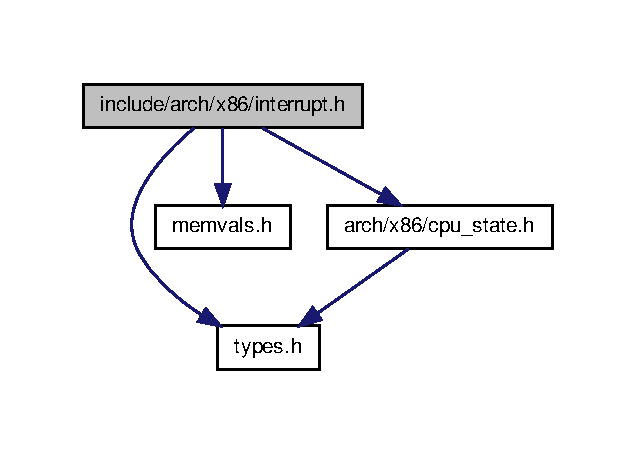
\includegraphics[width=305pt]{interrupt_8h__incl}
\end{center}
\end{figure}
\-This graph shows which files directly or indirectly include this file\-:\nopagebreak
\begin{figure}[H]
\begin{center}
\leavevmode
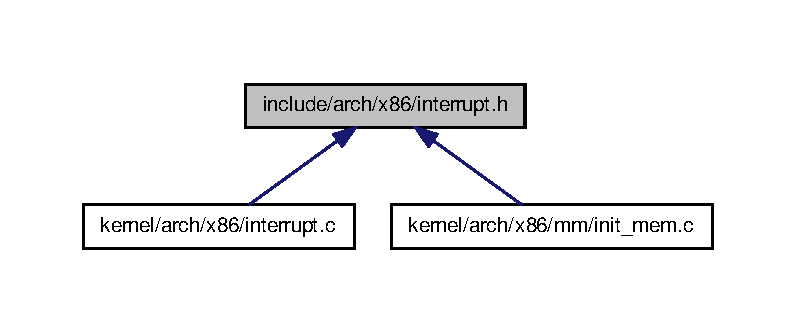
\includegraphics[width=350pt]{interrupt_8h__dep__incl}
\end{center}
\end{figure}
\subsection*{\-Data \-Structures}
\begin{DoxyCompactItemize}
\item 
struct \hyperlink{struct____attribute____}{\-\_\-\-\_\-attribute\-\_\-\-\_\-}
\end{DoxyCompactItemize}
\subsection*{\-Defines}
\begin{DoxyCompactItemize}
\item 
\#define \hyperlink{interrupt_8h_a1103a6e770fd3f28e321e0ff9eb0a259}{\-\_\-\-C\-A\-T\-E\-R\-N\-E\-L\-\_\-\-X86\-\_\-\-I\-N\-T\-E\-R\-R\-U\-P\-T\-\_\-\-H\-\_\-}
\item 
\#define \hyperlink{interrupt_8h_a2ed687a3ed1c8fe8709395b2563fddab}{\-G\-A\-T\-E\-\_\-\-T\-A\-S\-K}~0x5
\item 
\#define \hyperlink{interrupt_8h_a4254a801d49bf2213d100af57135e7f5}{\-G\-A\-T\-E\-\_\-\-I\-N\-T16}~0x6
\item 
\#define \hyperlink{interrupt_8h_acfc188f33a5983edae41807820e695d9}{\-G\-A\-T\-E\-\_\-\-T\-R\-A\-P16}~0x7
\item 
\#define \hyperlink{interrupt_8h_a5fdb56715285c2945f01fdd9e18098d3}{\-G\-A\-T\-E\-\_\-\-I\-N\-T32}~0x\-E
\item 
\#define \hyperlink{interrupt_8h_afa85551da9e066145b12bcab0d8e1271}{\-G\-A\-T\-E\-\_\-\-T\-R\-A\-P32}~0x\-F
\item 
\#define \hyperlink{interrupt_8h_a2a59a505aa55f15c152f30f811fbd310}{\-I\-D\-T\-\_\-\-E\-N\-T\-R\-I\-E\-S}~64
\item 
\#define \hyperlink{interrupt_8h_a94296a7edd74ed3be4462e2bb5c0f94f}{\-G\-A\-T\-E\-\_\-\-F\-I\-L\-L}(gate, type, dpl, sel, offset)
\item 
\#define \hyperlink{interrupt_8h_a5cddf66e6f0f966f2d935d55efe7aa7a}{\-V\-E\-C\-T\-O\-R\-\_\-\-I\-N\-D\-E\-X}(cnt)~vector\-\_\-\#\#cnt
\item 
\#define \hyperlink{interrupt_8h_aa7e12fffcbf53528a7e5e900ae7b4cb6}{\-G\-A\-T\-E\-\_\-\-O\-F\-F\-S\-E\-T}(gate, vector)
\item 
\#define \hyperlink{interrupt_8h_a80632065e2dcaae1447ea73103f4ad4f}{\-G\-P}~13
\item 
\#define \hyperlink{interrupt_8h_aa0e278c26c25558741febfadd7216caa}{\-P\-F}~14
\item 
\#define \hyperlink{interrupt_8h_ab491ed17f14e27a3f00f28dd0746d991}{\-P\-F\-\_\-\-V\-I\-O\-L\-A\-T\-I\-O\-N}~0x1
\item 
\#define \hyperlink{interrupt_8h_aaabc3980e39d66b82d53a40369124fa1}{\-P\-F\-\_\-\-N\-O\-T\-\_\-\-P\-R\-E\-S\-E\-N\-T}~$\sim$\hyperlink{interrupt_8h_ab491ed17f14e27a3f00f28dd0746d991}{\-P\-F\-\_\-\-V\-I\-O\-L\-A\-T\-I\-O\-N}
\item 
\#define \hyperlink{interrupt_8h_a070ef564933ae25764c5e1cb92172493}{\-P\-F\-\_\-\-O\-N\-\_\-\-W\-R\-I\-T\-E}~0x2
\item 
\#define \hyperlink{interrupt_8h_ab561c5c4a2281a8137a39e502e28b4f8}{\-P\-F\-\_\-\-O\-N\-\_\-\-R\-E\-A\-D}~$\sim$\hyperlink{interrupt_8h_a070ef564933ae25764c5e1cb92172493}{\-P\-F\-\_\-\-O\-N\-\_\-\-W\-R\-I\-T\-E}
\item 
\#define \hyperlink{interrupt_8h_af914450fde46a4ca9c3223570c0f5a0a}{\-P\-F\-\_\-\-F\-R\-O\-M\-\_\-\-U\-S\-E\-R}~0x4
\item 
\#define \hyperlink{interrupt_8h_aa02ce6202a631abadf40edf606ed0767}{\-P\-F\-\_\-\-F\-R\-O\-M\-\_\-\-K\-E\-R\-N\-E\-L}~$\sim$\hyperlink{interrupt_8h_af914450fde46a4ca9c3223570c0f5a0a}{\-P\-F\-\_\-\-F\-R\-O\-M\-\_\-\-U\-S\-E\-R}
\item 
\#define \hyperlink{interrupt_8h_a873bebeabe42214270bbf3698cfab80b}{\-P\-F\-\_\-\-I\-F\-E\-T\-C\-H}~0x10
\item 
\#define \hyperlink{interrupt_8h_a3444fa162af6afc32bbe7beffdedab61}{\-P\-F\-\_\-\-R\-S\-R\-V\-D}~0x8
\end{DoxyCompactItemize}
\subsection*{\-Typedefs}
\begin{DoxyCompactItemize}
\item 
typedef struct \hyperlink{structGdtdesc}{\-Gdtdesc} \hyperlink{interrupt_8h_a81398f7aecfca5502a385160a0f84f7a}{\-Idtdesc}
\end{DoxyCompactItemize}
\subsection*{\-Functions}
\begin{DoxyCompactItemize}
\item 
void \hyperlink{interrupt_8h_a164d38a0163ec2c36993b803b8c7fdcb}{idt\-\_\-init} (void)
\item 
void \hyperlink{interrupt_8h_ab836013c5b99083f285ae2326b3d0b3c}{map\-\_\-exception} (\hyperlink{types_8h_a435d1572bf3f880d55459d9805097f62}{uint32\-\_\-t}, \hyperlink{structcpu__state__t}{cpu\-\_\-state\-\_\-t} $\ast$)
\item 
\hyperlink{types_8h_a435d1572bf3f880d55459d9805097f62}{uint32\-\_\-t} \hyperlink{interrupt_8h_ab13687fc7d407eae4d97c68bfc410097}{page\-\_\-fault\-\_\-handler} (\hyperlink{structcpu__state__t}{cpu\-\_\-state\-\_\-t} $\ast$)
\end{DoxyCompactItemize}
\subsection*{\-Variables}
\begin{DoxyCompactItemize}
\item 
gatedesc \hyperlink{interrupt_8h_a5e84c643beec737df624fd986a319fbd}{idt} \mbox{[}$\,$\mbox{]}
\item 
char $\ast$ \hyperlink{interrupt_8h_a555133898405bfedf4422c9f76a58875}{x86\-\_\-exception\-\_\-names} \mbox{[}$\,$\mbox{]}
\end{DoxyCompactItemize}


\subsection{\-Define \-Documentation}
\hypertarget{interrupt_8h_a1103a6e770fd3f28e321e0ff9eb0a259}{\index{interrupt.\-h@{interrupt.\-h}!\-\_\-\-C\-A\-T\-E\-R\-N\-E\-L\-\_\-\-X86\-\_\-\-I\-N\-T\-E\-R\-R\-U\-P\-T\-\_\-\-H\-\_\-@{\-\_\-\-C\-A\-T\-E\-R\-N\-E\-L\-\_\-\-X86\-\_\-\-I\-N\-T\-E\-R\-R\-U\-P\-T\-\_\-\-H\-\_\-}}
\index{\-\_\-\-C\-A\-T\-E\-R\-N\-E\-L\-\_\-\-X86\-\_\-\-I\-N\-T\-E\-R\-R\-U\-P\-T\-\_\-\-H\-\_\-@{\-\_\-\-C\-A\-T\-E\-R\-N\-E\-L\-\_\-\-X86\-\_\-\-I\-N\-T\-E\-R\-R\-U\-P\-T\-\_\-\-H\-\_\-}!interrupt.h@{interrupt.\-h}}
\subsubsection[{\-\_\-\-C\-A\-T\-E\-R\-N\-E\-L\-\_\-\-X86\-\_\-\-I\-N\-T\-E\-R\-R\-U\-P\-T\-\_\-\-H\-\_\-}]{\setlength{\rightskip}{0pt plus 5cm}\#define {\bf \-\_\-\-C\-A\-T\-E\-R\-N\-E\-L\-\_\-\-X86\-\_\-\-I\-N\-T\-E\-R\-R\-U\-P\-T\-\_\-\-H\-\_\-}}}\label{interrupt_8h_a1103a6e770fd3f28e321e0ff9eb0a259}
\hyperlink{interrupt_8h}{include/arch/x86/interrupt.\-h} \-C\-A\-T\-Reloaded (\-C) \-Copyrights 2011 \href{http://catreloaded.net}{\tt http\-://catreloaded.\-net}

\begin{DoxyDate}{\-Date}
27 \-Sept, 2012 
\end{DoxyDate}


\-Definition at line 11 of file interrupt.\-h.

\hypertarget{interrupt_8h_a94296a7edd74ed3be4462e2bb5c0f94f}{\index{interrupt.\-h@{interrupt.\-h}!\-G\-A\-T\-E\-\_\-\-F\-I\-L\-L@{\-G\-A\-T\-E\-\_\-\-F\-I\-L\-L}}
\index{\-G\-A\-T\-E\-\_\-\-F\-I\-L\-L@{\-G\-A\-T\-E\-\_\-\-F\-I\-L\-L}!interrupt.h@{interrupt.\-h}}
\subsubsection[{\-G\-A\-T\-E\-\_\-\-F\-I\-L\-L}]{\setlength{\rightskip}{0pt plus 5cm}\#define {\bf \-G\-A\-T\-E\-\_\-\-F\-I\-L\-L}(
\begin{DoxyParamCaption}
\item[{}]{gate, }
\item[{}]{type, }
\item[{}]{dpl, }
\item[{}]{sel, }
\item[{}]{offset}
\end{DoxyParamCaption}
)}}\label{interrupt_8h_a94296a7edd74ed3be4462e2bb5c0f94f}
{\bfseries \-Value\-:}
\begin{DoxyCode}
\
        (gate)->offset_0_15 = (uint16_t)        ((offset) & 0xffff);    \
        (gate)->segment_s = (uint16_t) (sel);                   \
        (gate)->args    = 0;                                    \
        (gate)->reserved        = 0;                                    \
        (gate)->type    = 0xe;                                  \
        (gate)->dpl     = 0;                                    \
        (gate)->p       = 1;                                    \
        (gate)->offset_16_31 = (uint16_t) ((offset) >> 16);
\end{DoxyCode}


\-Definition at line 69 of file interrupt.\-h.

\hypertarget{interrupt_8h_a4254a801d49bf2213d100af57135e7f5}{\index{interrupt.\-h@{interrupt.\-h}!\-G\-A\-T\-E\-\_\-\-I\-N\-T16@{\-G\-A\-T\-E\-\_\-\-I\-N\-T16}}
\index{\-G\-A\-T\-E\-\_\-\-I\-N\-T16@{\-G\-A\-T\-E\-\_\-\-I\-N\-T16}!interrupt.h@{interrupt.\-h}}
\subsubsection[{\-G\-A\-T\-E\-\_\-\-I\-N\-T16}]{\setlength{\rightskip}{0pt plus 5cm}\#define {\bf \-G\-A\-T\-E\-\_\-\-I\-N\-T16}~0x6}}\label{interrupt_8h_a4254a801d49bf2213d100af57135e7f5}


\-Definition at line 58 of file interrupt.\-h.

\hypertarget{interrupt_8h_a5fdb56715285c2945f01fdd9e18098d3}{\index{interrupt.\-h@{interrupt.\-h}!\-G\-A\-T\-E\-\_\-\-I\-N\-T32@{\-G\-A\-T\-E\-\_\-\-I\-N\-T32}}
\index{\-G\-A\-T\-E\-\_\-\-I\-N\-T32@{\-G\-A\-T\-E\-\_\-\-I\-N\-T32}!interrupt.h@{interrupt.\-h}}
\subsubsection[{\-G\-A\-T\-E\-\_\-\-I\-N\-T32}]{\setlength{\rightskip}{0pt plus 5cm}\#define {\bf \-G\-A\-T\-E\-\_\-\-I\-N\-T32}~0x\-E}}\label{interrupt_8h_a5fdb56715285c2945f01fdd9e18098d3}


\-Definition at line 60 of file interrupt.\-h.

\hypertarget{interrupt_8h_aa7e12fffcbf53528a7e5e900ae7b4cb6}{\index{interrupt.\-h@{interrupt.\-h}!\-G\-A\-T\-E\-\_\-\-O\-F\-F\-S\-E\-T@{\-G\-A\-T\-E\-\_\-\-O\-F\-F\-S\-E\-T}}
\index{\-G\-A\-T\-E\-\_\-\-O\-F\-F\-S\-E\-T@{\-G\-A\-T\-E\-\_\-\-O\-F\-F\-S\-E\-T}!interrupt.h@{interrupt.\-h}}
\subsubsection[{\-G\-A\-T\-E\-\_\-\-O\-F\-F\-S\-E\-T}]{\setlength{\rightskip}{0pt plus 5cm}\#define {\bf \-G\-A\-T\-E\-\_\-\-O\-F\-F\-S\-E\-T}(
\begin{DoxyParamCaption}
\item[{}]{gate, }
\item[{}]{vector}
\end{DoxyParamCaption}
)}}\label{interrupt_8h_aa7e12fffcbf53528a7e5e900ae7b4cb6}
{\bfseries \-Value\-:}
\begin{DoxyCode}
(gate).offset_0_15 = (uint32_t) (((uint32_t) vector) & 0xffff);\
        (gate).offset_16_31= (uint32_t) (((uint32_t) vector) >> 16);
\end{DoxyCode}


\-Definition at line 87 of file interrupt.\-h.

\hypertarget{interrupt_8h_a2ed687a3ed1c8fe8709395b2563fddab}{\index{interrupt.\-h@{interrupt.\-h}!\-G\-A\-T\-E\-\_\-\-T\-A\-S\-K@{\-G\-A\-T\-E\-\_\-\-T\-A\-S\-K}}
\index{\-G\-A\-T\-E\-\_\-\-T\-A\-S\-K@{\-G\-A\-T\-E\-\_\-\-T\-A\-S\-K}!interrupt.h@{interrupt.\-h}}
\subsubsection[{\-G\-A\-T\-E\-\_\-\-T\-A\-S\-K}]{\setlength{\rightskip}{0pt plus 5cm}\#define {\bf \-G\-A\-T\-E\-\_\-\-T\-A\-S\-K}~0x5}}\label{interrupt_8h_a2ed687a3ed1c8fe8709395b2563fddab}


\-Definition at line 57 of file interrupt.\-h.

\hypertarget{interrupt_8h_acfc188f33a5983edae41807820e695d9}{\index{interrupt.\-h@{interrupt.\-h}!\-G\-A\-T\-E\-\_\-\-T\-R\-A\-P16@{\-G\-A\-T\-E\-\_\-\-T\-R\-A\-P16}}
\index{\-G\-A\-T\-E\-\_\-\-T\-R\-A\-P16@{\-G\-A\-T\-E\-\_\-\-T\-R\-A\-P16}!interrupt.h@{interrupt.\-h}}
\subsubsection[{\-G\-A\-T\-E\-\_\-\-T\-R\-A\-P16}]{\setlength{\rightskip}{0pt plus 5cm}\#define {\bf \-G\-A\-T\-E\-\_\-\-T\-R\-A\-P16}~0x7}}\label{interrupt_8h_acfc188f33a5983edae41807820e695d9}


\-Definition at line 59 of file interrupt.\-h.

\hypertarget{interrupt_8h_afa85551da9e066145b12bcab0d8e1271}{\index{interrupt.\-h@{interrupt.\-h}!\-G\-A\-T\-E\-\_\-\-T\-R\-A\-P32@{\-G\-A\-T\-E\-\_\-\-T\-R\-A\-P32}}
\index{\-G\-A\-T\-E\-\_\-\-T\-R\-A\-P32@{\-G\-A\-T\-E\-\_\-\-T\-R\-A\-P32}!interrupt.h@{interrupt.\-h}}
\subsubsection[{\-G\-A\-T\-E\-\_\-\-T\-R\-A\-P32}]{\setlength{\rightskip}{0pt plus 5cm}\#define {\bf \-G\-A\-T\-E\-\_\-\-T\-R\-A\-P32}~0x\-F}}\label{interrupt_8h_afa85551da9e066145b12bcab0d8e1271}


\-Definition at line 61 of file interrupt.\-h.

\hypertarget{interrupt_8h_a80632065e2dcaae1447ea73103f4ad4f}{\index{interrupt.\-h@{interrupt.\-h}!\-G\-P@{\-G\-P}}
\index{\-G\-P@{\-G\-P}!interrupt.h@{interrupt.\-h}}
\subsubsection[{\-G\-P}]{\setlength{\rightskip}{0pt plus 5cm}\#define {\bf \-G\-P}~13}}\label{interrupt_8h_a80632065e2dcaae1447ea73103f4ad4f}


\-Definition at line 92 of file interrupt.\-h.

\hypertarget{interrupt_8h_a2a59a505aa55f15c152f30f811fbd310}{\index{interrupt.\-h@{interrupt.\-h}!\-I\-D\-T\-\_\-\-E\-N\-T\-R\-I\-E\-S@{\-I\-D\-T\-\_\-\-E\-N\-T\-R\-I\-E\-S}}
\index{\-I\-D\-T\-\_\-\-E\-N\-T\-R\-I\-E\-S@{\-I\-D\-T\-\_\-\-E\-N\-T\-R\-I\-E\-S}!interrupt.h@{interrupt.\-h}}
\subsubsection[{\-I\-D\-T\-\_\-\-E\-N\-T\-R\-I\-E\-S}]{\setlength{\rightskip}{0pt plus 5cm}\#define {\bf \-I\-D\-T\-\_\-\-E\-N\-T\-R\-I\-E\-S}~64}}\label{interrupt_8h_a2a59a505aa55f15c152f30f811fbd310}


\-Definition at line 63 of file interrupt.\-h.

\hypertarget{interrupt_8h_aa0e278c26c25558741febfadd7216caa}{\index{interrupt.\-h@{interrupt.\-h}!\-P\-F@{\-P\-F}}
\index{\-P\-F@{\-P\-F}!interrupt.h@{interrupt.\-h}}
\subsubsection[{\-P\-F}]{\setlength{\rightskip}{0pt plus 5cm}\#define {\bf \-P\-F}~14}}\label{interrupt_8h_aa0e278c26c25558741febfadd7216caa}


\-Definition at line 93 of file interrupt.\-h.

\hypertarget{interrupt_8h_aa02ce6202a631abadf40edf606ed0767}{\index{interrupt.\-h@{interrupt.\-h}!\-P\-F\-\_\-\-F\-R\-O\-M\-\_\-\-K\-E\-R\-N\-E\-L@{\-P\-F\-\_\-\-F\-R\-O\-M\-\_\-\-K\-E\-R\-N\-E\-L}}
\index{\-P\-F\-\_\-\-F\-R\-O\-M\-\_\-\-K\-E\-R\-N\-E\-L@{\-P\-F\-\_\-\-F\-R\-O\-M\-\_\-\-K\-E\-R\-N\-E\-L}!interrupt.h@{interrupt.\-h}}
\subsubsection[{\-P\-F\-\_\-\-F\-R\-O\-M\-\_\-\-K\-E\-R\-N\-E\-L}]{\setlength{\rightskip}{0pt plus 5cm}\#define {\bf \-P\-F\-\_\-\-F\-R\-O\-M\-\_\-\-K\-E\-R\-N\-E\-L}~$\sim${\bf \-P\-F\-\_\-\-F\-R\-O\-M\-\_\-\-U\-S\-E\-R}}}\label{interrupt_8h_aa02ce6202a631abadf40edf606ed0767}


\-Definition at line 100 of file interrupt.\-h.

\hypertarget{interrupt_8h_af914450fde46a4ca9c3223570c0f5a0a}{\index{interrupt.\-h@{interrupt.\-h}!\-P\-F\-\_\-\-F\-R\-O\-M\-\_\-\-U\-S\-E\-R@{\-P\-F\-\_\-\-F\-R\-O\-M\-\_\-\-U\-S\-E\-R}}
\index{\-P\-F\-\_\-\-F\-R\-O\-M\-\_\-\-U\-S\-E\-R@{\-P\-F\-\_\-\-F\-R\-O\-M\-\_\-\-U\-S\-E\-R}!interrupt.h@{interrupt.\-h}}
\subsubsection[{\-P\-F\-\_\-\-F\-R\-O\-M\-\_\-\-U\-S\-E\-R}]{\setlength{\rightskip}{0pt plus 5cm}\#define {\bf \-P\-F\-\_\-\-F\-R\-O\-M\-\_\-\-U\-S\-E\-R}~0x4}}\label{interrupt_8h_af914450fde46a4ca9c3223570c0f5a0a}


\-Definition at line 99 of file interrupt.\-h.

\hypertarget{interrupt_8h_a873bebeabe42214270bbf3698cfab80b}{\index{interrupt.\-h@{interrupt.\-h}!\-P\-F\-\_\-\-I\-F\-E\-T\-C\-H@{\-P\-F\-\_\-\-I\-F\-E\-T\-C\-H}}
\index{\-P\-F\-\_\-\-I\-F\-E\-T\-C\-H@{\-P\-F\-\_\-\-I\-F\-E\-T\-C\-H}!interrupt.h@{interrupt.\-h}}
\subsubsection[{\-P\-F\-\_\-\-I\-F\-E\-T\-C\-H}]{\setlength{\rightskip}{0pt plus 5cm}\#define {\bf \-P\-F\-\_\-\-I\-F\-E\-T\-C\-H}~0x10}}\label{interrupt_8h_a873bebeabe42214270bbf3698cfab80b}


\-Definition at line 101 of file interrupt.\-h.

\hypertarget{interrupt_8h_aaabc3980e39d66b82d53a40369124fa1}{\index{interrupt.\-h@{interrupt.\-h}!\-P\-F\-\_\-\-N\-O\-T\-\_\-\-P\-R\-E\-S\-E\-N\-T@{\-P\-F\-\_\-\-N\-O\-T\-\_\-\-P\-R\-E\-S\-E\-N\-T}}
\index{\-P\-F\-\_\-\-N\-O\-T\-\_\-\-P\-R\-E\-S\-E\-N\-T@{\-P\-F\-\_\-\-N\-O\-T\-\_\-\-P\-R\-E\-S\-E\-N\-T}!interrupt.h@{interrupt.\-h}}
\subsubsection[{\-P\-F\-\_\-\-N\-O\-T\-\_\-\-P\-R\-E\-S\-E\-N\-T}]{\setlength{\rightskip}{0pt plus 5cm}\#define {\bf \-P\-F\-\_\-\-N\-O\-T\-\_\-\-P\-R\-E\-S\-E\-N\-T}~$\sim${\bf \-P\-F\-\_\-\-V\-I\-O\-L\-A\-T\-I\-O\-N}}}\label{interrupt_8h_aaabc3980e39d66b82d53a40369124fa1}


\-Definition at line 96 of file interrupt.\-h.

\hypertarget{interrupt_8h_ab561c5c4a2281a8137a39e502e28b4f8}{\index{interrupt.\-h@{interrupt.\-h}!\-P\-F\-\_\-\-O\-N\-\_\-\-R\-E\-A\-D@{\-P\-F\-\_\-\-O\-N\-\_\-\-R\-E\-A\-D}}
\index{\-P\-F\-\_\-\-O\-N\-\_\-\-R\-E\-A\-D@{\-P\-F\-\_\-\-O\-N\-\_\-\-R\-E\-A\-D}!interrupt.h@{interrupt.\-h}}
\subsubsection[{\-P\-F\-\_\-\-O\-N\-\_\-\-R\-E\-A\-D}]{\setlength{\rightskip}{0pt plus 5cm}\#define {\bf \-P\-F\-\_\-\-O\-N\-\_\-\-R\-E\-A\-D}~$\sim${\bf \-P\-F\-\_\-\-O\-N\-\_\-\-W\-R\-I\-T\-E}}}\label{interrupt_8h_ab561c5c4a2281a8137a39e502e28b4f8}


\-Definition at line 98 of file interrupt.\-h.

\hypertarget{interrupt_8h_a070ef564933ae25764c5e1cb92172493}{\index{interrupt.\-h@{interrupt.\-h}!\-P\-F\-\_\-\-O\-N\-\_\-\-W\-R\-I\-T\-E@{\-P\-F\-\_\-\-O\-N\-\_\-\-W\-R\-I\-T\-E}}
\index{\-P\-F\-\_\-\-O\-N\-\_\-\-W\-R\-I\-T\-E@{\-P\-F\-\_\-\-O\-N\-\_\-\-W\-R\-I\-T\-E}!interrupt.h@{interrupt.\-h}}
\subsubsection[{\-P\-F\-\_\-\-O\-N\-\_\-\-W\-R\-I\-T\-E}]{\setlength{\rightskip}{0pt plus 5cm}\#define {\bf \-P\-F\-\_\-\-O\-N\-\_\-\-W\-R\-I\-T\-E}~0x2}}\label{interrupt_8h_a070ef564933ae25764c5e1cb92172493}


\-Definition at line 97 of file interrupt.\-h.

\hypertarget{interrupt_8h_a3444fa162af6afc32bbe7beffdedab61}{\index{interrupt.\-h@{interrupt.\-h}!\-P\-F\-\_\-\-R\-S\-R\-V\-D@{\-P\-F\-\_\-\-R\-S\-R\-V\-D}}
\index{\-P\-F\-\_\-\-R\-S\-R\-V\-D@{\-P\-F\-\_\-\-R\-S\-R\-V\-D}!interrupt.h@{interrupt.\-h}}
\subsubsection[{\-P\-F\-\_\-\-R\-S\-R\-V\-D}]{\setlength{\rightskip}{0pt plus 5cm}\#define {\bf \-P\-F\-\_\-\-R\-S\-R\-V\-D}~0x8}}\label{interrupt_8h_a3444fa162af6afc32bbe7beffdedab61}


\-Definition at line 102 of file interrupt.\-h.

\hypertarget{interrupt_8h_ab491ed17f14e27a3f00f28dd0746d991}{\index{interrupt.\-h@{interrupt.\-h}!\-P\-F\-\_\-\-V\-I\-O\-L\-A\-T\-I\-O\-N@{\-P\-F\-\_\-\-V\-I\-O\-L\-A\-T\-I\-O\-N}}
\index{\-P\-F\-\_\-\-V\-I\-O\-L\-A\-T\-I\-O\-N@{\-P\-F\-\_\-\-V\-I\-O\-L\-A\-T\-I\-O\-N}!interrupt.h@{interrupt.\-h}}
\subsubsection[{\-P\-F\-\_\-\-V\-I\-O\-L\-A\-T\-I\-O\-N}]{\setlength{\rightskip}{0pt plus 5cm}\#define {\bf \-P\-F\-\_\-\-V\-I\-O\-L\-A\-T\-I\-O\-N}~0x1}}\label{interrupt_8h_ab491ed17f14e27a3f00f28dd0746d991}


\-Definition at line 95 of file interrupt.\-h.

\hypertarget{interrupt_8h_a5cddf66e6f0f966f2d935d55efe7aa7a}{\index{interrupt.\-h@{interrupt.\-h}!\-V\-E\-C\-T\-O\-R\-\_\-\-I\-N\-D\-E\-X@{\-V\-E\-C\-T\-O\-R\-\_\-\-I\-N\-D\-E\-X}}
\index{\-V\-E\-C\-T\-O\-R\-\_\-\-I\-N\-D\-E\-X@{\-V\-E\-C\-T\-O\-R\-\_\-\-I\-N\-D\-E\-X}!interrupt.h@{interrupt.\-h}}
\subsubsection[{\-V\-E\-C\-T\-O\-R\-\_\-\-I\-N\-D\-E\-X}]{\setlength{\rightskip}{0pt plus 5cm}\#define {\bf \-V\-E\-C\-T\-O\-R\-\_\-\-I\-N\-D\-E\-X}(
\begin{DoxyParamCaption}
\item[{}]{cnt}
\end{DoxyParamCaption}
)~vector\-\_\-\#\#cnt}}\label{interrupt_8h_a5cddf66e6f0f966f2d935d55efe7aa7a}


\-Definition at line 85 of file interrupt.\-h.



\subsection{\-Typedef \-Documentation}
\hypertarget{interrupt_8h_a81398f7aecfca5502a385160a0f84f7a}{\index{interrupt.\-h@{interrupt.\-h}!\-Idtdesc@{\-Idtdesc}}
\index{\-Idtdesc@{\-Idtdesc}!interrupt.h@{interrupt.\-h}}
\subsubsection[{\-Idtdesc}]{\setlength{\rightskip}{0pt plus 5cm}typedef struct {\bf \-Gdtdesc} {\bf \-Idtdesc}}}\label{interrupt_8h_a81398f7aecfca5502a385160a0f84f7a}


\-Definition at line 48 of file interrupt.\-h.



\subsection{\-Function \-Documentation}
\hypertarget{interrupt_8h_a164d38a0163ec2c36993b803b8c7fdcb}{\index{interrupt.\-h@{interrupt.\-h}!idt\-\_\-init@{idt\-\_\-init}}
\index{idt\-\_\-init@{idt\-\_\-init}!interrupt.h@{interrupt.\-h}}
\subsubsection[{idt\-\_\-init}]{\setlength{\rightskip}{0pt plus 5cm}void {\bf idt\-\_\-init} (
\begin{DoxyParamCaption}
\item[{void}]{}
\end{DoxyParamCaption}
)}}\label{interrupt_8h_a164d38a0163ec2c36993b803b8c7fdcb}


\-Definition at line 60 of file interrupt.\-c.

\hypertarget{interrupt_8h_ab836013c5b99083f285ae2326b3d0b3c}{\index{interrupt.\-h@{interrupt.\-h}!map\-\_\-exception@{map\-\_\-exception}}
\index{map\-\_\-exception@{map\-\_\-exception}!interrupt.h@{interrupt.\-h}}
\subsubsection[{map\-\_\-exception}]{\setlength{\rightskip}{0pt plus 5cm}void {\bf map\-\_\-exception} (
\begin{DoxyParamCaption}
\item[{{\bf uint32\-\_\-t}}]{, }
\item[{{\bf cpu\-\_\-state\-\_\-t} $\ast$}]{}
\end{DoxyParamCaption}
)}}\label{interrupt_8h_ab836013c5b99083f285ae2326b3d0b3c}


\-Definition at line 166 of file interrupt.\-c.

\hypertarget{interrupt_8h_ab13687fc7d407eae4d97c68bfc410097}{\index{interrupt.\-h@{interrupt.\-h}!page\-\_\-fault\-\_\-handler@{page\-\_\-fault\-\_\-handler}}
\index{page\-\_\-fault\-\_\-handler@{page\-\_\-fault\-\_\-handler}!interrupt.h@{interrupt.\-h}}
\subsubsection[{page\-\_\-fault\-\_\-handler}]{\setlength{\rightskip}{0pt plus 5cm}{\bf uint32\-\_\-t} {\bf page\-\_\-fault\-\_\-handler} (
\begin{DoxyParamCaption}
\item[{{\bf cpu\-\_\-state\-\_\-t} $\ast$}]{}
\end{DoxyParamCaption}
)}}\label{interrupt_8h_ab13687fc7d407eae4d97c68bfc410097}


\-Definition at line 195 of file interrupt.\-c.



\subsection{\-Variable \-Documentation}
\hypertarget{interrupt_8h_a5e84c643beec737df624fd986a319fbd}{\index{interrupt.\-h@{interrupt.\-h}!idt@{idt}}
\index{idt@{idt}!interrupt.h@{interrupt.\-h}}
\subsubsection[{idt}]{\setlength{\rightskip}{0pt plus 5cm}gatedesc {\bf idt}\mbox{[}$\,$\mbox{]}}}\label{interrupt_8h_a5e84c643beec737df624fd986a319fbd}
\hyperlink{interrupt_8h}{include/arch/x86/interrupt.\-h} \-C\-A\-T\-Reloaded (\-C) \-Copyrights 2011 \href{http://catreloaded.net}{\tt http\-://catreloaded.\-net}

\begin{DoxyDate}{\-Date}
27 \-Sept, 2012 
\end{DoxyDate}


\-Definition at line 107 of file interrupt.\-h.

\hypertarget{interrupt_8h_a555133898405bfedf4422c9f76a58875}{\index{interrupt.\-h@{interrupt.\-h}!x86\-\_\-exception\-\_\-names@{x86\-\_\-exception\-\_\-names}}
\index{x86\-\_\-exception\-\_\-names@{x86\-\_\-exception\-\_\-names}!interrupt.h@{interrupt.\-h}}
\subsubsection[{x86\-\_\-exception\-\_\-names}]{\setlength{\rightskip}{0pt plus 5cm}char$\ast$ {\bf x86\-\_\-exception\-\_\-names}\mbox{[}$\,$\mbox{]}}}\label{interrupt_8h_a555133898405bfedf4422c9f76a58875}


\-Definition at line 20 of file interrupt.\-c.


\hypertarget{page_8h}{\section{include/arch/x86/mm/page.h \-File \-Reference}
\label{page_8h}\index{include/arch/x86/mm/page.\-h@{include/arch/x86/mm/page.\-h}}
}
{\ttfamily \#include $<$structs/linkedlist.\-h$>$}\*
{\ttfamily \#include $<$memvals.\-h$>$}\*
{\ttfamily \#include $<$test.\-h$>$}\*
\-Include dependency graph for page.\-h\-:\nopagebreak
\begin{figure}[H]
\begin{center}
\leavevmode
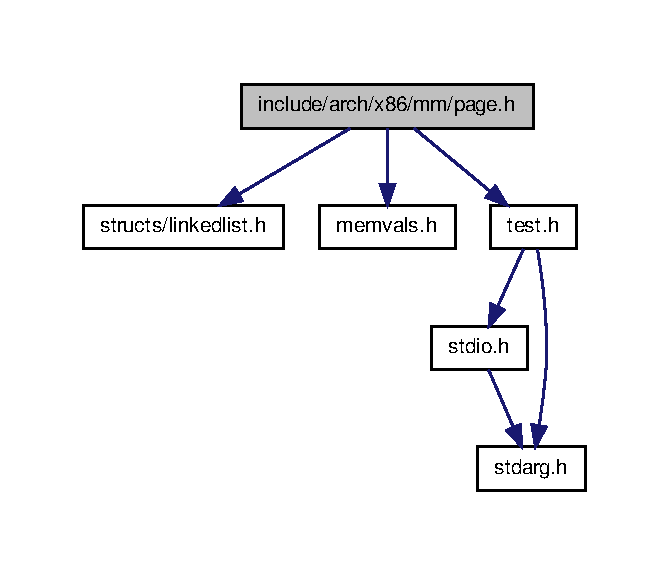
\includegraphics[width=321pt]{page_8h__incl}
\end{center}
\end{figure}
\-This graph shows which files directly or indirectly include this file\-:\nopagebreak
\begin{figure}[H]
\begin{center}
\leavevmode
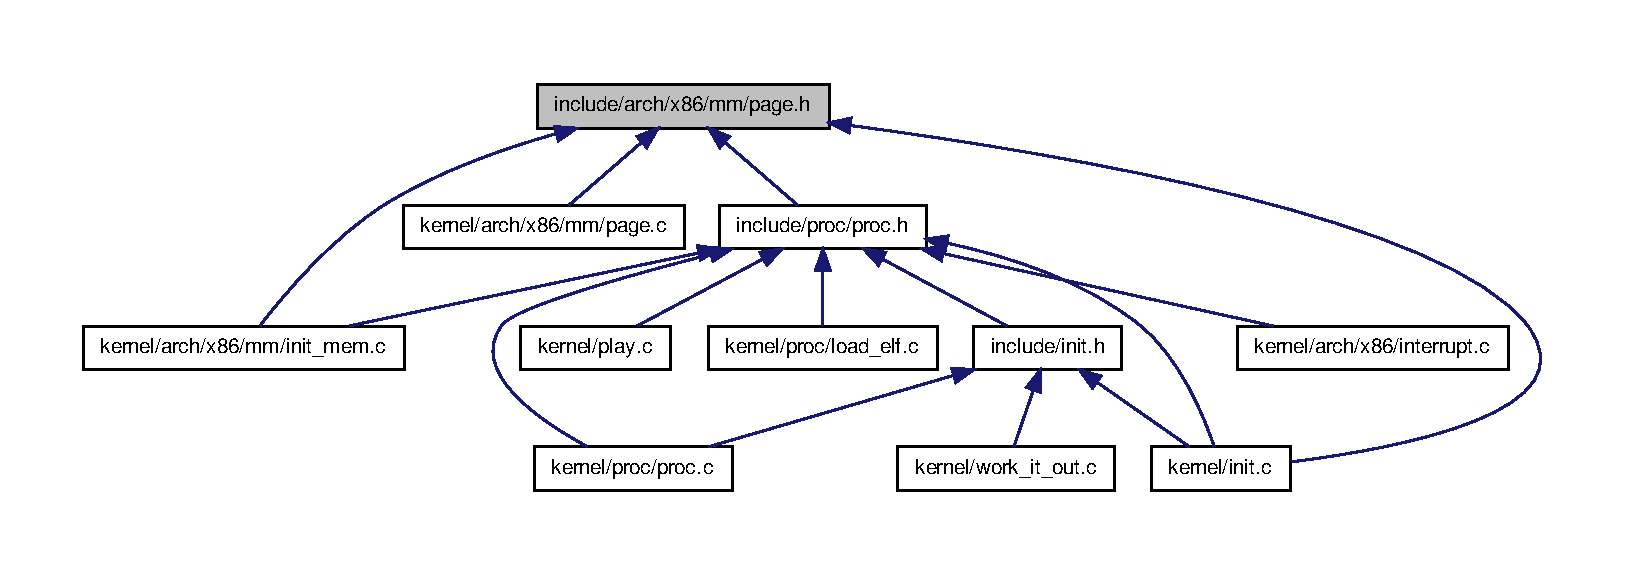
\includegraphics[width=350pt]{page_8h__dep__incl}
\end{center}
\end{figure}
\subsection*{\-Data \-Structures}
\begin{DoxyCompactItemize}
\item 
struct \hyperlink{struct____attribute____}{\-\_\-\-\_\-attribute\-\_\-\-\_\-}
\item 
struct \hyperlink{structPage}{\-Page}
\end{DoxyCompactItemize}
\subsection*{\-Defines}
\begin{DoxyCompactItemize}
\item 
\#define \hyperlink{page_8h_a122dfc414a40e260fd35dbe9743db26f}{\-P\-A\-G\-E\-\_\-\-P\-R\-E\-S\-E\-N\-T}~0x1
\item 
\#define \hyperlink{page_8h_a80a2168882aa2c8cf95fa34edb75ec4d}{\-P\-A\-G\-E\-\_\-\-W\-R\-I\-T\-A\-B\-L\-E}~0x2
\item 
\#define \hyperlink{page_8h_a2d0253527ea5080d6befe0ee3bde473f}{\-P\-A\-G\-E\-\_\-\-U\-S\-E\-R}~0x4
\item 
\#define \hyperlink{page_8h_abee2fa55ece4424017eaedd401f653db}{\-P\-A\-G\-E\-\_\-\-W\-T\-H\-R\-O\-U\-G\-H}~0x8
\item 
\#define \hyperlink{page_8h_a931f4fae9a466305f8d1e36693b64ed9}{\-P\-A\-G\-E\-\_\-\-C\-D\-I\-S\-A\-B\-L\-E}~0x10
\item 
\#define \hyperlink{page_8h_add0f255a15cf72f5b47251d19092c41d}{\-P\-A\-G\-E\-\_\-\-A\-C\-C\-E\-S\-S\-E\-D}~0x20
\item 
\#define \hyperlink{page_8h_a0b65338140b4aab20aae2708677df343}{\-P\-A\-G\-E\-\_\-\-D\-I\-R\-T\-Y}~0x40
\item 
\#define \hyperlink{page_8h_a0b65338140b4aab20aae2708677df343}{\-P\-A\-G\-E\-\_\-\-D\-I\-R\-T\-Y}~0x40
\item 
\#define \hyperlink{page_8h_a0d99c75e51b448fcb97266da4815c63f}{\-P\-A\-G\-E\-\_\-\-G\-L\-O\-B\-A\-L}~0x100
\item 
\#define \hyperlink{page_8h_a7c1b222c8ae46edef4d04bcbdbbd7a65}{\-P\-A\-G\-E\-\_\-\-P\-A\-G\-E\-S\-Z}~0x80
\item 
\#define \hyperlink{page_8h_af1dce3fb288c323b42a528c06c2deb32}{\-P\-G\-T\-B\-L\-\_\-\-S\-H\-I\-F\-T}~12
\item 
\#define \hyperlink{page_8h_a75ee8179ce74ddb3af9df418bfbca263}{\-P\-G\-D\-I\-R\-\_\-\-S\-H\-I\-F\-T}~22
\item 
\#define \hyperlink{page_8h_a20d0b7c5f64f21a3fdc19cf44afe8ff2}{\-P\-G\-S\-H\-I\-F\-T}~12
\item 
\#define \hyperlink{page_8h_a2c15062f44b5767fd4be9a8d399ee3d9}{\-P\-T\-S\-H\-I\-F\-T}~22
\item 
\#define \hyperlink{page_8h_a8ae633afbe67c2bc60876a0d9b30aa50}{\-P\-G\-D\-I\-R\-X}(lin)~(( ((\hyperlink{types_8h_a435d1572bf3f880d55459d9805097f62}{uint32\-\_\-t})(lin)) $>$$>$ \hyperlink{page_8h_a75ee8179ce74ddb3af9df418bfbca263}{\-P\-G\-D\-I\-R\-\_\-\-S\-H\-I\-F\-T}) \& 0x3\-F\-F)
\item 
\#define \hyperlink{page_8h_afc904a4b66602cfaeffd7bf9ec1e1b33}{\-V\-I\-R\-T\-\_\-\-P\-G\-D\-I\-R\-X}(lin)~\hyperlink{page_8h_a8ae633afbe67c2bc60876a0d9b30aa50}{\-P\-G\-D\-I\-R\-X}((lin))
\item 
\#define \hyperlink{page_8h_a10438b55704a14378c9936f0b661c74f}{\-P\-G\-T\-B\-L\-X}(lin)~(( ((\hyperlink{types_8h_a435d1572bf3f880d55459d9805097f62}{uint32\-\_\-t})(lin)) $>$$>$ \hyperlink{page_8h_af1dce3fb288c323b42a528c06c2deb32}{\-P\-G\-T\-B\-L\-\_\-\-S\-H\-I\-F\-T}) \& 0x3\-F\-F)
\item 
\#define \hyperlink{page_8h_a9ff2d4222c4941bcfc737d00cac2b7c9}{\-V\-I\-R\-T\-\_\-\-P\-G\-T\-B\-L\-X}(lin)~\hyperlink{page_8h_a10438b55704a14378c9936f0b661c74f}{\-P\-G\-T\-B\-L\-X}((lin))
\item 
\#define \hyperlink{page_8h_acc35e6016ef18bc23a9d2206572a9658}{\-P\-G\-P\-N}(lin)~(((\hyperlink{types_8h_a435d1572bf3f880d55459d9805097f62}{uint32\-\_\-t})(lin)) $>$$>$ \hyperlink{page_8h_af1dce3fb288c323b42a528c06c2deb32}{\-P\-G\-T\-B\-L\-\_\-\-S\-H\-I\-F\-T})
\item 
\#define \hyperlink{page_8h_a1e6c03f6df7c26497ee380658b4834ee}{\-V\-I\-R\-T\-\_\-\-P\-G\-P\-N}(lin)~\hyperlink{page_8h_acc35e6016ef18bc23a9d2206572a9658}{\-P\-G\-P\-N}((lin))
\item 
\#define \hyperlink{page_8h_aa619f31c4093d2c4e30cdf22d4cd7f40}{\-P\-G\-O\-F\-F}(lin)~(( (lin) \& 0x\-F\-F\-F))
\item 
\#define \hyperlink{page_8h_a75787dd0e9092079fdd5e40e6aaff2f1}{\-P\-T\-D\-\_\-\-A\-D\-D\-R}(lin)~(( (\hyperlink{types_8h_a435d1572bf3f880d55459d9805097f62}{uint32\-\_\-t}) (lin)) \& $\sim$0x\-F\-F\-F)
\item 
\#define \hyperlink{page_8h_a92a2e483e7b710c68ce330535b947c24}{\-P\-A2\-K\-A}(pa)
\item 
\#define \hyperlink{page_8h_a03aed022a2d4770c017f55d6f072d300}{\-K\-A2\-P\-A}(va)
\end{DoxyCompactItemize}
\subsection*{\-Typedefs}
\begin{DoxyCompactItemize}
\item 
typedef \hyperlink{types_8h_a435d1572bf3f880d55459d9805097f62}{uint32\-\_\-t} \hyperlink{page_8h_a1ae9855ac82633447ab53f25e49e1f62}{pde\-\_\-t}
\end{DoxyCompactItemize}
\subsection*{\-Functions}
\begin{DoxyCompactItemize}
\item 
static \hyperlink{types_8h_a9f047c1f0917f6184a7a013d4b4277a6}{paddr\-\_\-t} \hyperlink{page_8h_abb8c2eff60eda24a85bcf989f661c13a}{va2pa} (\hyperlink{page_8h_a1ae9855ac82633447ab53f25e49e1f62}{pde\-\_\-t} $\ast$pgdir, void $\ast$va)
\item 
\hyperlink{page_8h_a5e8075b44a75674bd656be86fdf4bd73}{\-L\-I\-S\-T\-\_\-\-H\-E\-A\-D} (\-Page\-List, \hyperlink{structPage}{\-Page})
\item 
typedef \hyperlink{page_8h_af06dbf095a0a3cb262f4ee59b32c6c7b}{\-L\-I\-S\-T\-\_\-\-E\-N\-T\-R\-Y} (\hyperlink{structPage}{\-Page}) page\-\_\-entry\-\_\-t
\item 
static \hyperlink{types_8h_a435d1572bf3f880d55459d9805097f62}{uint32\-\_\-t} \hyperlink{page_8h_a735b55b2c43127444f76fd10f474f8c9}{pagetoppn} (struct \hyperlink{structPage}{\-Page} $\ast$p)
\item 
static void $\ast$ \hyperlink{page_8h_a3ba1dbb29838d112343f5c3ca65bd22e}{patopage} (\hyperlink{types_8h_a9f047c1f0917f6184a7a013d4b4277a6}{paddr\-\_\-t} p)
\item 
static \hyperlink{types_8h_a9f047c1f0917f6184a7a013d4b4277a6}{paddr\-\_\-t} \hyperlink{page_8h_ab6c946403ac4ab350ca9a5b12ec08f5b}{pagetopa} (struct \hyperlink{structPage}{\-Page} $\ast$p)
\item 
static void $\ast$ \hyperlink{page_8h_a94dd2ec22e115460a6d568f22ebd91c2}{pagetova} (struct \hyperlink{structPage}{\-Page} $\ast$p)
\item 
void \hyperlink{page_8h_a3116202f5e2264b63f5a69f007287b9a}{x86\-\_\-paging\-\_\-init} (void)
\item 
void \hyperlink{page_8h_a11e80d1cc051516c82574218cd4d8a2e}{x86\-\_\-page\-\_\-init} (struct \hyperlink{structPage}{\-Page} $\ast$)
\item 
int \hyperlink{page_8h_aade2e8ac5c3f45d00dd3cfed120ce06e}{x86\-\_\-page\-\_\-alloc} (struct \hyperlink{structPage}{\-Page} $\ast$$\ast$)
\item 
void \hyperlink{page_8h_a6839239bf39164211468ee9ced0f56c9}{x86\-\_\-page\-\_\-free} (struct \hyperlink{structPage}{\-Page} $\ast$)
\item 
void \hyperlink{page_8h_a4cfcd3f4ec83fe65d87fdf84687fcea7}{x86\-\_\-page\-\_\-detach} (struct \hyperlink{structPage}{\-Page} $\ast$)
\item 
pte\-\_\-t $\ast$ \hyperlink{page_8h_a5a77f74c19e12b42ae6ac430a1da67f3}{x86\-\_\-pgdir\-\_\-find} (\hyperlink{page_8h_a1ae9855ac82633447ab53f25e49e1f62}{pde\-\_\-t} $\ast$, const void $\ast$, int)
\item 
struct \hyperlink{structPage}{\-Page} $\ast$ \hyperlink{page_8h_aabbe2a1888b08c852a59e98a894184d6}{x86\-\_\-page\-\_\-lookup} (\hyperlink{page_8h_a1ae9855ac82633447ab53f25e49e1f62}{pde\-\_\-t} $\ast$, void $\ast$, pte\-\_\-t $\ast$$\ast$)
\item 
void \hyperlink{page_8h_a54da2098233e8e95613fbe8d474ccb6e}{x86\-\_\-page\-\_\-remove} (\hyperlink{page_8h_a1ae9855ac82633447ab53f25e49e1f62}{pde\-\_\-t} $\ast$, void $\ast$)
\item 
int \hyperlink{page_8h_a039ec961f11b8a99073285dd66aa249f}{x86\-\_\-page\-\_\-insert} (\hyperlink{page_8h_a1ae9855ac82633447ab53f25e49e1f62}{pde\-\_\-t} $\ast$, struct \hyperlink{structPage}{\-Page} $\ast$, void $\ast$, \hyperlink{types_8h_a435d1572bf3f880d55459d9805097f62}{uint32\-\_\-t})
\item 
void \hyperlink{page_8h_a890b33877bfdb45d1c074589b4b94adb}{map\-\_\-segment\-\_\-page} (\hyperlink{page_8h_a1ae9855ac82633447ab53f25e49e1f62}{pde\-\_\-t} $\ast$, \hyperlink{types_8h_a53428b953a0ae6fba02a5b3596c867e0}{vaddr\-\_\-t}, \hyperlink{types_8h_a7c94ea6f8948649f8d181ae55911eeaf}{size\-\_\-t}, \hyperlink{types_8h_a9f047c1f0917f6184a7a013d4b4277a6}{paddr\-\_\-t}, int)
\item 
void \hyperlink{page_8h_a3c2de2a5079f7f0854f1e2df482dbd99}{x86\-\_\-test\-\_\-pgdir} (void)
\item 
void \hyperlink{page_8h_ad25003f0037fee68d8baaa0b273a5f1c}{x86\-\_\-test\-\_\-paging} (void)
\item 
static void \hyperlink{page_8h_a0fa97889e8b26d5b543bad604635cf68}{x86\-\_\-test\-\_\-page\-\_\-alloc} (void)
\end{DoxyCompactItemize}
\subsection*{\-Variables}
\begin{DoxyCompactItemize}
\item 
\hyperlink{types_8h_a7c94ea6f8948649f8d181ae55911eeaf}{size\-\_\-t} \hyperlink{page_8h_aa0a18b4e3e172dc4a506562989bbaf70}{page\-\_\-count}
\item 
volatile pte\-\_\-t \hyperlink{page_8h_a544646a9bbfa46f498ab151f5812bc07}{virtpgt} \mbox{[}$\,$\mbox{]}
\item 
volatile \hyperlink{page_8h_a1ae9855ac82633447ab53f25e49e1f62}{pde\-\_\-t} \hyperlink{page_8h_ac7011e2a2096dd3c6d03729bbfaeaf88}{virtpgd} \mbox{[}$\,$\mbox{]}
\item 
char \hyperlink{page_8h_a07f1c8c8948d648a82059e75458b27b9}{kernel\-\_\-stack} \mbox{[}$\,$\mbox{]}
\item 
char \hyperlink{page_8h_a07c8861d848ab5f43efb105f7d95e4da}{kernel\-\_\-stack\-\_\-end} \mbox{[}$\,$\mbox{]}
\item 
struct \hyperlink{structPage}{\-Page} $\ast$ \hyperlink{page_8h_a5c8561a52c4cda29a9be7dc7be92c771}{pages}
\item 
\hyperlink{types_8h_a435d1572bf3f880d55459d9805097f62}{uint32\-\_\-t} \hyperlink{page_8h_a18cb6aa9c5285aa7411ebd96a283741e}{global\-\_\-cr3}
\item 
\hyperlink{page_8h_a1ae9855ac82633447ab53f25e49e1f62}{pde\-\_\-t} $\ast$ \hyperlink{page_8h_a8ffe8b80013a018b23501ea7a45b7870}{global\-\_\-pgdir}
\item 
struct \hyperlink{structSegdesc}{\-Segdesc} \hyperlink{page_8h_ab4d4fde7a5a671b7c81db7a24059acf5}{gdt} \mbox{[}$\,$\mbox{]}
\item 
char $\ast$ \hyperlink{page_8h_a39aa9990303c751420729e015f952dfb}{next\-\_\-free}
\end{DoxyCompactItemize}


\subsection{\-Define \-Documentation}
\hypertarget{page_8h_a03aed022a2d4770c017f55d6f072d300}{\index{page.\-h@{page.\-h}!\-K\-A2\-P\-A@{\-K\-A2\-P\-A}}
\index{\-K\-A2\-P\-A@{\-K\-A2\-P\-A}!page.h@{page.\-h}}
\subsubsection[{\-K\-A2\-P\-A}]{\setlength{\rightskip}{0pt plus 5cm}\#define {\bf \-K\-A2\-P\-A}(
\begin{DoxyParamCaption}
\item[{}]{va}
\end{DoxyParamCaption}
)}}\label{page_8h_a03aed022a2d4770c017f55d6f072d300}
{\bfseries \-Value\-:}
\begin{DoxyCode}
({                                      \
        vaddr_t m_va = (vaddr_t) (va);  \
        if( m_va < KERNEL_ADDR){\
                panic("KA2PA called with bad address \n");\
        }\
        m_va - KERNEL_ADDR;\
})
\end{DoxyCode}


\-Definition at line 90 of file page.\-h.

\hypertarget{page_8h_a92a2e483e7b710c68ce330535b947c24}{\index{page.\-h@{page.\-h}!\-P\-A2\-K\-A@{\-P\-A2\-K\-A}}
\index{\-P\-A2\-K\-A@{\-P\-A2\-K\-A}!page.h@{page.\-h}}
\subsubsection[{\-P\-A2\-K\-A}]{\setlength{\rightskip}{0pt plus 5cm}\#define {\bf \-P\-A2\-K\-A}(
\begin{DoxyParamCaption}
\item[{}]{pa}
\end{DoxyParamCaption}
)}}\label{page_8h_a92a2e483e7b710c68ce330535b947c24}
{\bfseries \-Value\-:}
\begin{DoxyCode}
({                                      \
        paddr_t m_pa = ((paddr_t) pa);  \
        paddr_t m_ppn = PGPN(m_pa);     \
        if( m_ppn >= page_count){       \
                panic("PA2KA called with invalid paddr\n");\
                }                       \
        (void *) (m_pa + KERNEL_ADDR);  \
})
\end{DoxyCode}


\-Definition at line 80 of file page.\-h.

\hypertarget{page_8h_add0f255a15cf72f5b47251d19092c41d}{\index{page.\-h@{page.\-h}!\-P\-A\-G\-E\-\_\-\-A\-C\-C\-E\-S\-S\-E\-D@{\-P\-A\-G\-E\-\_\-\-A\-C\-C\-E\-S\-S\-E\-D}}
\index{\-P\-A\-G\-E\-\_\-\-A\-C\-C\-E\-S\-S\-E\-D@{\-P\-A\-G\-E\-\_\-\-A\-C\-C\-E\-S\-S\-E\-D}!page.h@{page.\-h}}
\subsubsection[{\-P\-A\-G\-E\-\_\-\-A\-C\-C\-E\-S\-S\-E\-D}]{\setlength{\rightskip}{0pt plus 5cm}\#define {\bf \-P\-A\-G\-E\-\_\-\-A\-C\-C\-E\-S\-S\-E\-D}~0x20}}\label{page_8h_add0f255a15cf72f5b47251d19092c41d}


\-Definition at line 47 of file page.\-h.

\hypertarget{page_8h_a931f4fae9a466305f8d1e36693b64ed9}{\index{page.\-h@{page.\-h}!\-P\-A\-G\-E\-\_\-\-C\-D\-I\-S\-A\-B\-L\-E@{\-P\-A\-G\-E\-\_\-\-C\-D\-I\-S\-A\-B\-L\-E}}
\index{\-P\-A\-G\-E\-\_\-\-C\-D\-I\-S\-A\-B\-L\-E@{\-P\-A\-G\-E\-\_\-\-C\-D\-I\-S\-A\-B\-L\-E}!page.h@{page.\-h}}
\subsubsection[{\-P\-A\-G\-E\-\_\-\-C\-D\-I\-S\-A\-B\-L\-E}]{\setlength{\rightskip}{0pt plus 5cm}\#define {\bf \-P\-A\-G\-E\-\_\-\-C\-D\-I\-S\-A\-B\-L\-E}~0x10}}\label{page_8h_a931f4fae9a466305f8d1e36693b64ed9}


\-Definition at line 46 of file page.\-h.

\hypertarget{page_8h_a0b65338140b4aab20aae2708677df343}{\index{page.\-h@{page.\-h}!\-P\-A\-G\-E\-\_\-\-D\-I\-R\-T\-Y@{\-P\-A\-G\-E\-\_\-\-D\-I\-R\-T\-Y}}
\index{\-P\-A\-G\-E\-\_\-\-D\-I\-R\-T\-Y@{\-P\-A\-G\-E\-\_\-\-D\-I\-R\-T\-Y}!page.h@{page.\-h}}
\subsubsection[{\-P\-A\-G\-E\-\_\-\-D\-I\-R\-T\-Y}]{\setlength{\rightskip}{0pt plus 5cm}\#define {\bf \-P\-A\-G\-E\-\_\-\-D\-I\-R\-T\-Y}~0x40}}\label{page_8h_a0b65338140b4aab20aae2708677df343}


\-Definition at line 51 of file page.\-h.

\hypertarget{page_8h_a0b65338140b4aab20aae2708677df343}{\index{page.\-h@{page.\-h}!\-P\-A\-G\-E\-\_\-\-D\-I\-R\-T\-Y@{\-P\-A\-G\-E\-\_\-\-D\-I\-R\-T\-Y}}
\index{\-P\-A\-G\-E\-\_\-\-D\-I\-R\-T\-Y@{\-P\-A\-G\-E\-\_\-\-D\-I\-R\-T\-Y}!page.h@{page.\-h}}
\subsubsection[{\-P\-A\-G\-E\-\_\-\-D\-I\-R\-T\-Y}]{\setlength{\rightskip}{0pt plus 5cm}\#define {\bf \-P\-A\-G\-E\-\_\-\-D\-I\-R\-T\-Y}~0x40}}\label{page_8h_a0b65338140b4aab20aae2708677df343}


\-Definition at line 51 of file page.\-h.

\hypertarget{page_8h_a0d99c75e51b448fcb97266da4815c63f}{\index{page.\-h@{page.\-h}!\-P\-A\-G\-E\-\_\-\-G\-L\-O\-B\-A\-L@{\-P\-A\-G\-E\-\_\-\-G\-L\-O\-B\-A\-L}}
\index{\-P\-A\-G\-E\-\_\-\-G\-L\-O\-B\-A\-L@{\-P\-A\-G\-E\-\_\-\-G\-L\-O\-B\-A\-L}!page.h@{page.\-h}}
\subsubsection[{\-P\-A\-G\-E\-\_\-\-G\-L\-O\-B\-A\-L}]{\setlength{\rightskip}{0pt plus 5cm}\#define {\bf \-P\-A\-G\-E\-\_\-\-G\-L\-O\-B\-A\-L}~0x100}}\label{page_8h_a0d99c75e51b448fcb97266da4815c63f}


\-Definition at line 52 of file page.\-h.

\hypertarget{page_8h_a7c1b222c8ae46edef4d04bcbdbbd7a65}{\index{page.\-h@{page.\-h}!\-P\-A\-G\-E\-\_\-\-P\-A\-G\-E\-S\-Z@{\-P\-A\-G\-E\-\_\-\-P\-A\-G\-E\-S\-Z}}
\index{\-P\-A\-G\-E\-\_\-\-P\-A\-G\-E\-S\-Z@{\-P\-A\-G\-E\-\_\-\-P\-A\-G\-E\-S\-Z}!page.h@{page.\-h}}
\subsubsection[{\-P\-A\-G\-E\-\_\-\-P\-A\-G\-E\-S\-Z}]{\setlength{\rightskip}{0pt plus 5cm}\#define {\bf \-P\-A\-G\-E\-\_\-\-P\-A\-G\-E\-S\-Z}~0x80}}\label{page_8h_a7c1b222c8ae46edef4d04bcbdbbd7a65}


\-Definition at line 55 of file page.\-h.

\hypertarget{page_8h_a122dfc414a40e260fd35dbe9743db26f}{\index{page.\-h@{page.\-h}!\-P\-A\-G\-E\-\_\-\-P\-R\-E\-S\-E\-N\-T@{\-P\-A\-G\-E\-\_\-\-P\-R\-E\-S\-E\-N\-T}}
\index{\-P\-A\-G\-E\-\_\-\-P\-R\-E\-S\-E\-N\-T@{\-P\-A\-G\-E\-\_\-\-P\-R\-E\-S\-E\-N\-T}!page.h@{page.\-h}}
\subsubsection[{\-P\-A\-G\-E\-\_\-\-P\-R\-E\-S\-E\-N\-T}]{\setlength{\rightskip}{0pt plus 5cm}\#define {\bf \-P\-A\-G\-E\-\_\-\-P\-R\-E\-S\-E\-N\-T}~0x1}}\label{page_8h_a122dfc414a40e260fd35dbe9743db26f}


\-Definition at line 42 of file page.\-h.

\hypertarget{page_8h_a2d0253527ea5080d6befe0ee3bde473f}{\index{page.\-h@{page.\-h}!\-P\-A\-G\-E\-\_\-\-U\-S\-E\-R@{\-P\-A\-G\-E\-\_\-\-U\-S\-E\-R}}
\index{\-P\-A\-G\-E\-\_\-\-U\-S\-E\-R@{\-P\-A\-G\-E\-\_\-\-U\-S\-E\-R}!page.h@{page.\-h}}
\subsubsection[{\-P\-A\-G\-E\-\_\-\-U\-S\-E\-R}]{\setlength{\rightskip}{0pt plus 5cm}\#define {\bf \-P\-A\-G\-E\-\_\-\-U\-S\-E\-R}~0x4}}\label{page_8h_a2d0253527ea5080d6befe0ee3bde473f}


\-Definition at line 44 of file page.\-h.

\hypertarget{page_8h_a80a2168882aa2c8cf95fa34edb75ec4d}{\index{page.\-h@{page.\-h}!\-P\-A\-G\-E\-\_\-\-W\-R\-I\-T\-A\-B\-L\-E@{\-P\-A\-G\-E\-\_\-\-W\-R\-I\-T\-A\-B\-L\-E}}
\index{\-P\-A\-G\-E\-\_\-\-W\-R\-I\-T\-A\-B\-L\-E@{\-P\-A\-G\-E\-\_\-\-W\-R\-I\-T\-A\-B\-L\-E}!page.h@{page.\-h}}
\subsubsection[{\-P\-A\-G\-E\-\_\-\-W\-R\-I\-T\-A\-B\-L\-E}]{\setlength{\rightskip}{0pt plus 5cm}\#define {\bf \-P\-A\-G\-E\-\_\-\-W\-R\-I\-T\-A\-B\-L\-E}~0x2}}\label{page_8h_a80a2168882aa2c8cf95fa34edb75ec4d}


\-Definition at line 43 of file page.\-h.

\hypertarget{page_8h_abee2fa55ece4424017eaedd401f653db}{\index{page.\-h@{page.\-h}!\-P\-A\-G\-E\-\_\-\-W\-T\-H\-R\-O\-U\-G\-H@{\-P\-A\-G\-E\-\_\-\-W\-T\-H\-R\-O\-U\-G\-H}}
\index{\-P\-A\-G\-E\-\_\-\-W\-T\-H\-R\-O\-U\-G\-H@{\-P\-A\-G\-E\-\_\-\-W\-T\-H\-R\-O\-U\-G\-H}!page.h@{page.\-h}}
\subsubsection[{\-P\-A\-G\-E\-\_\-\-W\-T\-H\-R\-O\-U\-G\-H}]{\setlength{\rightskip}{0pt plus 5cm}\#define {\bf \-P\-A\-G\-E\-\_\-\-W\-T\-H\-R\-O\-U\-G\-H}~0x8}}\label{page_8h_abee2fa55ece4424017eaedd401f653db}


\-Definition at line 45 of file page.\-h.

\hypertarget{page_8h_a75ee8179ce74ddb3af9df418bfbca263}{\index{page.\-h@{page.\-h}!\-P\-G\-D\-I\-R\-\_\-\-S\-H\-I\-F\-T@{\-P\-G\-D\-I\-R\-\_\-\-S\-H\-I\-F\-T}}
\index{\-P\-G\-D\-I\-R\-\_\-\-S\-H\-I\-F\-T@{\-P\-G\-D\-I\-R\-\_\-\-S\-H\-I\-F\-T}!page.h@{page.\-h}}
\subsubsection[{\-P\-G\-D\-I\-R\-\_\-\-S\-H\-I\-F\-T}]{\setlength{\rightskip}{0pt plus 5cm}\#define {\bf \-P\-G\-D\-I\-R\-\_\-\-S\-H\-I\-F\-T}~22}}\label{page_8h_a75ee8179ce74ddb3af9df418bfbca263}


\-Definition at line 59 of file page.\-h.

\hypertarget{page_8h_a8ae633afbe67c2bc60876a0d9b30aa50}{\index{page.\-h@{page.\-h}!\-P\-G\-D\-I\-R\-X@{\-P\-G\-D\-I\-R\-X}}
\index{\-P\-G\-D\-I\-R\-X@{\-P\-G\-D\-I\-R\-X}!page.h@{page.\-h}}
\subsubsection[{\-P\-G\-D\-I\-R\-X}]{\setlength{\rightskip}{0pt plus 5cm}\#define {\bf \-P\-G\-D\-I\-R\-X}(
\begin{DoxyParamCaption}
\item[{}]{lin}
\end{DoxyParamCaption}
)~(( (({\bf uint32\-\_\-t})(lin)) $>$$>$ {\bf \-P\-G\-D\-I\-R\-\_\-\-S\-H\-I\-F\-T}) \& 0x3\-F\-F)}}\label{page_8h_a8ae633afbe67c2bc60876a0d9b30aa50}


\-Definition at line 64 of file page.\-h.

\hypertarget{page_8h_aa619f31c4093d2c4e30cdf22d4cd7f40}{\index{page.\-h@{page.\-h}!\-P\-G\-O\-F\-F@{\-P\-G\-O\-F\-F}}
\index{\-P\-G\-O\-F\-F@{\-P\-G\-O\-F\-F}!page.h@{page.\-h}}
\subsubsection[{\-P\-G\-O\-F\-F}]{\setlength{\rightskip}{0pt plus 5cm}\#define {\bf \-P\-G\-O\-F\-F}(
\begin{DoxyParamCaption}
\item[{}]{lin}
\end{DoxyParamCaption}
)~(( (lin) \& 0x\-F\-F\-F))}}\label{page_8h_aa619f31c4093d2c4e30cdf22d4cd7f40}


\-Definition at line 73 of file page.\-h.

\hypertarget{page_8h_acc35e6016ef18bc23a9d2206572a9658}{\index{page.\-h@{page.\-h}!\-P\-G\-P\-N@{\-P\-G\-P\-N}}
\index{\-P\-G\-P\-N@{\-P\-G\-P\-N}!page.h@{page.\-h}}
\subsubsection[{\-P\-G\-P\-N}]{\setlength{\rightskip}{0pt plus 5cm}\#define {\bf \-P\-G\-P\-N}(
\begin{DoxyParamCaption}
\item[{}]{lin}
\end{DoxyParamCaption}
)~((({\bf uint32\-\_\-t})(lin)) $>$$>$ {\bf \-P\-G\-T\-B\-L\-\_\-\-S\-H\-I\-F\-T})}}\label{page_8h_acc35e6016ef18bc23a9d2206572a9658}


\-Definition at line 70 of file page.\-h.

\hypertarget{page_8h_a20d0b7c5f64f21a3fdc19cf44afe8ff2}{\index{page.\-h@{page.\-h}!\-P\-G\-S\-H\-I\-F\-T@{\-P\-G\-S\-H\-I\-F\-T}}
\index{\-P\-G\-S\-H\-I\-F\-T@{\-P\-G\-S\-H\-I\-F\-T}!page.h@{page.\-h}}
\subsubsection[{\-P\-G\-S\-H\-I\-F\-T}]{\setlength{\rightskip}{0pt plus 5cm}\#define {\bf \-P\-G\-S\-H\-I\-F\-T}~12}}\label{page_8h_a20d0b7c5f64f21a3fdc19cf44afe8ff2}


\-Definition at line 60 of file page.\-h.

\hypertarget{page_8h_af1dce3fb288c323b42a528c06c2deb32}{\index{page.\-h@{page.\-h}!\-P\-G\-T\-B\-L\-\_\-\-S\-H\-I\-F\-T@{\-P\-G\-T\-B\-L\-\_\-\-S\-H\-I\-F\-T}}
\index{\-P\-G\-T\-B\-L\-\_\-\-S\-H\-I\-F\-T@{\-P\-G\-T\-B\-L\-\_\-\-S\-H\-I\-F\-T}!page.h@{page.\-h}}
\subsubsection[{\-P\-G\-T\-B\-L\-\_\-\-S\-H\-I\-F\-T}]{\setlength{\rightskip}{0pt plus 5cm}\#define {\bf \-P\-G\-T\-B\-L\-\_\-\-S\-H\-I\-F\-T}~12}}\label{page_8h_af1dce3fb288c323b42a528c06c2deb32}


\-Definition at line 58 of file page.\-h.

\hypertarget{page_8h_a10438b55704a14378c9936f0b661c74f}{\index{page.\-h@{page.\-h}!\-P\-G\-T\-B\-L\-X@{\-P\-G\-T\-B\-L\-X}}
\index{\-P\-G\-T\-B\-L\-X@{\-P\-G\-T\-B\-L\-X}!page.h@{page.\-h}}
\subsubsection[{\-P\-G\-T\-B\-L\-X}]{\setlength{\rightskip}{0pt plus 5cm}\#define {\bf \-P\-G\-T\-B\-L\-X}(
\begin{DoxyParamCaption}
\item[{}]{lin}
\end{DoxyParamCaption}
)~(( (({\bf uint32\-\_\-t})(lin)) $>$$>$ {\bf \-P\-G\-T\-B\-L\-\_\-\-S\-H\-I\-F\-T}) \& 0x3\-F\-F)}}\label{page_8h_a10438b55704a14378c9936f0b661c74f}


\-Definition at line 67 of file page.\-h.

\hypertarget{page_8h_a75787dd0e9092079fdd5e40e6aaff2f1}{\index{page.\-h@{page.\-h}!\-P\-T\-D\-\_\-\-A\-D\-D\-R@{\-P\-T\-D\-\_\-\-A\-D\-D\-R}}
\index{\-P\-T\-D\-\_\-\-A\-D\-D\-R@{\-P\-T\-D\-\_\-\-A\-D\-D\-R}!page.h@{page.\-h}}
\subsubsection[{\-P\-T\-D\-\_\-\-A\-D\-D\-R}]{\setlength{\rightskip}{0pt plus 5cm}\#define {\bf \-P\-T\-D\-\_\-\-A\-D\-D\-R}(
\begin{DoxyParamCaption}
\item[{}]{lin}
\end{DoxyParamCaption}
)~(( ({\bf uint32\-\_\-t}) (lin)) \& $\sim$0x\-F\-F\-F)}}\label{page_8h_a75787dd0e9092079fdd5e40e6aaff2f1}


\-Definition at line 74 of file page.\-h.

\hypertarget{page_8h_a2c15062f44b5767fd4be9a8d399ee3d9}{\index{page.\-h@{page.\-h}!\-P\-T\-S\-H\-I\-F\-T@{\-P\-T\-S\-H\-I\-F\-T}}
\index{\-P\-T\-S\-H\-I\-F\-T@{\-P\-T\-S\-H\-I\-F\-T}!page.h@{page.\-h}}
\subsubsection[{\-P\-T\-S\-H\-I\-F\-T}]{\setlength{\rightskip}{0pt plus 5cm}\#define {\bf \-P\-T\-S\-H\-I\-F\-T}~22}}\label{page_8h_a2c15062f44b5767fd4be9a8d399ee3d9}


\-Definition at line 61 of file page.\-h.

\hypertarget{page_8h_afc904a4b66602cfaeffd7bf9ec1e1b33}{\index{page.\-h@{page.\-h}!\-V\-I\-R\-T\-\_\-\-P\-G\-D\-I\-R\-X@{\-V\-I\-R\-T\-\_\-\-P\-G\-D\-I\-R\-X}}
\index{\-V\-I\-R\-T\-\_\-\-P\-G\-D\-I\-R\-X@{\-V\-I\-R\-T\-\_\-\-P\-G\-D\-I\-R\-X}!page.h@{page.\-h}}
\subsubsection[{\-V\-I\-R\-T\-\_\-\-P\-G\-D\-I\-R\-X}]{\setlength{\rightskip}{0pt plus 5cm}\#define {\bf \-V\-I\-R\-T\-\_\-\-P\-G\-D\-I\-R\-X}(
\begin{DoxyParamCaption}
\item[{}]{lin}
\end{DoxyParamCaption}
)~{\bf \-P\-G\-D\-I\-R\-X}((lin))}}\label{page_8h_afc904a4b66602cfaeffd7bf9ec1e1b33}


\-Definition at line 65 of file page.\-h.

\hypertarget{page_8h_a1e6c03f6df7c26497ee380658b4834ee}{\index{page.\-h@{page.\-h}!\-V\-I\-R\-T\-\_\-\-P\-G\-P\-N@{\-V\-I\-R\-T\-\_\-\-P\-G\-P\-N}}
\index{\-V\-I\-R\-T\-\_\-\-P\-G\-P\-N@{\-V\-I\-R\-T\-\_\-\-P\-G\-P\-N}!page.h@{page.\-h}}
\subsubsection[{\-V\-I\-R\-T\-\_\-\-P\-G\-P\-N}]{\setlength{\rightskip}{0pt plus 5cm}\#define {\bf \-V\-I\-R\-T\-\_\-\-P\-G\-P\-N}(
\begin{DoxyParamCaption}
\item[{}]{lin}
\end{DoxyParamCaption}
)~{\bf \-P\-G\-P\-N}((lin))}}\label{page_8h_a1e6c03f6df7c26497ee380658b4834ee}


\-Definition at line 71 of file page.\-h.

\hypertarget{page_8h_a9ff2d4222c4941bcfc737d00cac2b7c9}{\index{page.\-h@{page.\-h}!\-V\-I\-R\-T\-\_\-\-P\-G\-T\-B\-L\-X@{\-V\-I\-R\-T\-\_\-\-P\-G\-T\-B\-L\-X}}
\index{\-V\-I\-R\-T\-\_\-\-P\-G\-T\-B\-L\-X@{\-V\-I\-R\-T\-\_\-\-P\-G\-T\-B\-L\-X}!page.h@{page.\-h}}
\subsubsection[{\-V\-I\-R\-T\-\_\-\-P\-G\-T\-B\-L\-X}]{\setlength{\rightskip}{0pt plus 5cm}\#define {\bf \-V\-I\-R\-T\-\_\-\-P\-G\-T\-B\-L\-X}(
\begin{DoxyParamCaption}
\item[{}]{lin}
\end{DoxyParamCaption}
)~{\bf \-P\-G\-T\-B\-L\-X}((lin))}}\label{page_8h_a9ff2d4222c4941bcfc737d00cac2b7c9}


\-Definition at line 68 of file page.\-h.



\subsection{\-Typedef \-Documentation}
\hypertarget{page_8h_a1ae9855ac82633447ab53f25e49e1f62}{\index{page.\-h@{page.\-h}!pde\-\_\-t@{pde\-\_\-t}}
\index{pde\-\_\-t@{pde\-\_\-t}!page.h@{page.\-h}}
\subsubsection[{pde\-\_\-t}]{\setlength{\rightskip}{0pt plus 5cm}typedef {\bf uint32\-\_\-t} {\bf pde\-\_\-t}}}\label{page_8h_a1ae9855ac82633447ab53f25e49e1f62}


\-Definition at line 25 of file page.\-h.



\subsection{\-Function \-Documentation}
\hypertarget{page_8h_af06dbf095a0a3cb262f4ee59b32c6c7b}{\index{page.\-h@{page.\-h}!\-L\-I\-S\-T\-\_\-\-E\-N\-T\-R\-Y@{\-L\-I\-S\-T\-\_\-\-E\-N\-T\-R\-Y}}
\index{\-L\-I\-S\-T\-\_\-\-E\-N\-T\-R\-Y@{\-L\-I\-S\-T\-\_\-\-E\-N\-T\-R\-Y}!page.h@{page.\-h}}
\subsubsection[{\-L\-I\-S\-T\-\_\-\-E\-N\-T\-R\-Y}]{\setlength{\rightskip}{0pt plus 5cm}typedef {\bf \-L\-I\-S\-T\-\_\-\-E\-N\-T\-R\-Y} (
\begin{DoxyParamCaption}
\item[{{\bf \-Page}}]{}
\end{DoxyParamCaption}
)}}\label{page_8h_af06dbf095a0a3cb262f4ee59b32c6c7b}
\hypertarget{page_8h_a5e8075b44a75674bd656be86fdf4bd73}{\index{page.\-h@{page.\-h}!\-L\-I\-S\-T\-\_\-\-H\-E\-A\-D@{\-L\-I\-S\-T\-\_\-\-H\-E\-A\-D}}
\index{\-L\-I\-S\-T\-\_\-\-H\-E\-A\-D@{\-L\-I\-S\-T\-\_\-\-H\-E\-A\-D}!page.h@{page.\-h}}
\subsubsection[{\-L\-I\-S\-T\-\_\-\-H\-E\-A\-D}]{\setlength{\rightskip}{0pt plus 5cm}{\bf \-L\-I\-S\-T\-\_\-\-H\-E\-A\-D} (
\begin{DoxyParamCaption}
\item[{\-Page\-List}]{, }
\item[{{\bf \-Page}}]{}
\end{DoxyParamCaption}
)}}\label{page_8h_a5e8075b44a75674bd656be86fdf4bd73}
\hypertarget{page_8h_a890b33877bfdb45d1c074589b4b94adb}{\index{page.\-h@{page.\-h}!map\-\_\-segment\-\_\-page@{map\-\_\-segment\-\_\-page}}
\index{map\-\_\-segment\-\_\-page@{map\-\_\-segment\-\_\-page}!page.h@{page.\-h}}
\subsubsection[{map\-\_\-segment\-\_\-page}]{\setlength{\rightskip}{0pt plus 5cm}void {\bf map\-\_\-segment\-\_\-page} (
\begin{DoxyParamCaption}
\item[{{\bf pde\-\_\-t} $\ast$}]{, }
\item[{{\bf vaddr\-\_\-t}}]{, }
\item[{{\bf size\-\_\-t}}]{, }
\item[{{\bf paddr\-\_\-t}}]{, }
\item[{int}]{}
\end{DoxyParamCaption}
)}}\label{page_8h_a890b33877bfdb45d1c074589b4b94adb}


\-Definition at line 231 of file page.\-c.

\hypertarget{page_8h_ab6c946403ac4ab350ca9a5b12ec08f5b}{\index{page.\-h@{page.\-h}!pagetopa@{pagetopa}}
\index{pagetopa@{pagetopa}!page.h@{page.\-h}}
\subsubsection[{pagetopa}]{\setlength{\rightskip}{0pt plus 5cm}static {\bf paddr\-\_\-t} {\bf pagetopa} (
\begin{DoxyParamCaption}
\item[{struct {\bf \-Page} $\ast$}]{p}
\end{DoxyParamCaption}
)\hspace{0.3cm}{\ttfamily  \mbox{[}inline, static\mbox{]}}}}\label{page_8h_ab6c946403ac4ab350ca9a5b12ec08f5b}


\-Definition at line 219 of file page.\-h.

\hypertarget{page_8h_a735b55b2c43127444f76fd10f474f8c9}{\index{page.\-h@{page.\-h}!pagetoppn@{pagetoppn}}
\index{pagetoppn@{pagetoppn}!page.h@{page.\-h}}
\subsubsection[{pagetoppn}]{\setlength{\rightskip}{0pt plus 5cm}static {\bf uint32\-\_\-t} {\bf pagetoppn} (
\begin{DoxyParamCaption}
\item[{struct {\bf \-Page} $\ast$}]{p}
\end{DoxyParamCaption}
)\hspace{0.3cm}{\ttfamily  \mbox{[}inline, static\mbox{]}}}}\label{page_8h_a735b55b2c43127444f76fd10f474f8c9}


\-Definition at line 197 of file page.\-h.

\hypertarget{page_8h_a94dd2ec22e115460a6d568f22ebd91c2}{\index{page.\-h@{page.\-h}!pagetova@{pagetova}}
\index{pagetova@{pagetova}!page.h@{page.\-h}}
\subsubsection[{pagetova}]{\setlength{\rightskip}{0pt plus 5cm}static void$\ast$ {\bf pagetova} (
\begin{DoxyParamCaption}
\item[{struct {\bf \-Page} $\ast$}]{p}
\end{DoxyParamCaption}
)\hspace{0.3cm}{\ttfamily  \mbox{[}inline, static\mbox{]}}}}\label{page_8h_a94dd2ec22e115460a6d568f22ebd91c2}


\-Definition at line 224 of file page.\-h.

\hypertarget{page_8h_a3ba1dbb29838d112343f5c3ca65bd22e}{\index{page.\-h@{page.\-h}!patopage@{patopage}}
\index{patopage@{patopage}!page.h@{page.\-h}}
\subsubsection[{patopage}]{\setlength{\rightskip}{0pt plus 5cm}static void$\ast$ {\bf patopage} (
\begin{DoxyParamCaption}
\item[{{\bf paddr\-\_\-t}}]{p}
\end{DoxyParamCaption}
)\hspace{0.3cm}{\ttfamily  \mbox{[}inline, static\mbox{]}}}}\label{page_8h_a3ba1dbb29838d112343f5c3ca65bd22e}


\-Definition at line 206 of file page.\-h.

\hypertarget{page_8h_abb8c2eff60eda24a85bcf989f661c13a}{\index{page.\-h@{page.\-h}!va2pa@{va2pa}}
\index{va2pa@{va2pa}!page.h@{page.\-h}}
\subsubsection[{va2pa}]{\setlength{\rightskip}{0pt plus 5cm}static {\bf paddr\-\_\-t} {\bf va2pa} (
\begin{DoxyParamCaption}
\item[{{\bf pde\-\_\-t} $\ast$}]{pgdir, }
\item[{void $\ast$}]{va}
\end{DoxyParamCaption}
)\hspace{0.3cm}{\ttfamily  \mbox{[}inline, static\mbox{]}}}}\label{page_8h_abb8c2eff60eda24a85bcf989f661c13a}


\-Definition at line 118 of file page.\-h.

\hypertarget{page_8h_aade2e8ac5c3f45d00dd3cfed120ce06e}{\index{page.\-h@{page.\-h}!x86\-\_\-page\-\_\-alloc@{x86\-\_\-page\-\_\-alloc}}
\index{x86\-\_\-page\-\_\-alloc@{x86\-\_\-page\-\_\-alloc}!page.h@{page.\-h}}
\subsubsection[{x86\-\_\-page\-\_\-alloc}]{\setlength{\rightskip}{0pt plus 5cm}int {\bf x86\-\_\-page\-\_\-alloc} (
\begin{DoxyParamCaption}
\item[{struct {\bf \-Page} $\ast$$\ast$}]{}
\end{DoxyParamCaption}
)}}\label{page_8h_aade2e8ac5c3f45d00dd3cfed120ce06e}


\-Definition at line 83 of file page.\-c.

\hypertarget{page_8h_a4cfcd3f4ec83fe65d87fdf84687fcea7}{\index{page.\-h@{page.\-h}!x86\-\_\-page\-\_\-detach@{x86\-\_\-page\-\_\-detach}}
\index{x86\-\_\-page\-\_\-detach@{x86\-\_\-page\-\_\-detach}!page.h@{page.\-h}}
\subsubsection[{x86\-\_\-page\-\_\-detach}]{\setlength{\rightskip}{0pt plus 5cm}void {\bf x86\-\_\-page\-\_\-detach} (
\begin{DoxyParamCaption}
\item[{struct {\bf \-Page} $\ast$}]{}
\end{DoxyParamCaption}
)}}\label{page_8h_a4cfcd3f4ec83fe65d87fdf84687fcea7}


\-Definition at line 112 of file page.\-c.

\hypertarget{page_8h_a6839239bf39164211468ee9ced0f56c9}{\index{page.\-h@{page.\-h}!x86\-\_\-page\-\_\-free@{x86\-\_\-page\-\_\-free}}
\index{x86\-\_\-page\-\_\-free@{x86\-\_\-page\-\_\-free}!page.h@{page.\-h}}
\subsubsection[{x86\-\_\-page\-\_\-free}]{\setlength{\rightskip}{0pt plus 5cm}void {\bf x86\-\_\-page\-\_\-free} (
\begin{DoxyParamCaption}
\item[{struct {\bf \-Page} $\ast$}]{}
\end{DoxyParamCaption}
)}}\label{page_8h_a6839239bf39164211468ee9ced0f56c9}


\-Definition at line 100 of file page.\-c.

\hypertarget{page_8h_a11e80d1cc051516c82574218cd4d8a2e}{\index{page.\-h@{page.\-h}!x86\-\_\-page\-\_\-init@{x86\-\_\-page\-\_\-init}}
\index{x86\-\_\-page\-\_\-init@{x86\-\_\-page\-\_\-init}!page.h@{page.\-h}}
\subsubsection[{x86\-\_\-page\-\_\-init}]{\setlength{\rightskip}{0pt plus 5cm}void {\bf x86\-\_\-page\-\_\-init} (
\begin{DoxyParamCaption}
\item[{struct {\bf \-Page} $\ast$}]{}
\end{DoxyParamCaption}
)}}\label{page_8h_a11e80d1cc051516c82574218cd4d8a2e}


\-Definition at line 74 of file page.\-c.

\hypertarget{page_8h_a039ec961f11b8a99073285dd66aa249f}{\index{page.\-h@{page.\-h}!x86\-\_\-page\-\_\-insert@{x86\-\_\-page\-\_\-insert}}
\index{x86\-\_\-page\-\_\-insert@{x86\-\_\-page\-\_\-insert}!page.h@{page.\-h}}
\subsubsection[{x86\-\_\-page\-\_\-insert}]{\setlength{\rightskip}{0pt plus 5cm}int {\bf x86\-\_\-page\-\_\-insert} (
\begin{DoxyParamCaption}
\item[{{\bf pde\-\_\-t} $\ast$}]{, }
\item[{struct {\bf \-Page} $\ast$}]{, }
\item[{void $\ast$}]{, }
\item[{{\bf uint32\-\_\-t}}]{}
\end{DoxyParamCaption}
)}}\label{page_8h_a039ec961f11b8a99073285dd66aa249f}


\-Definition at line 184 of file page.\-c.

\hypertarget{page_8h_aabbe2a1888b08c852a59e98a894184d6}{\index{page.\-h@{page.\-h}!x86\-\_\-page\-\_\-lookup@{x86\-\_\-page\-\_\-lookup}}
\index{x86\-\_\-page\-\_\-lookup@{x86\-\_\-page\-\_\-lookup}!page.h@{page.\-h}}
\subsubsection[{x86\-\_\-page\-\_\-lookup}]{\setlength{\rightskip}{0pt plus 5cm}struct {\bf \-Page}$\ast$ {\bf x86\-\_\-page\-\_\-lookup} (
\begin{DoxyParamCaption}
\item[{{\bf pde\-\_\-t} $\ast$}]{, }
\item[{void $\ast$}]{, }
\item[{pte\-\_\-t $\ast$$\ast$}]{}
\end{DoxyParamCaption}
)\hspace{0.3cm}{\ttfamily  \mbox{[}read\mbox{]}}}}\label{page_8h_aabbe2a1888b08c852a59e98a894184d6}


\-Definition at line 154 of file page.\-c.

\hypertarget{page_8h_a54da2098233e8e95613fbe8d474ccb6e}{\index{page.\-h@{page.\-h}!x86\-\_\-page\-\_\-remove@{x86\-\_\-page\-\_\-remove}}
\index{x86\-\_\-page\-\_\-remove@{x86\-\_\-page\-\_\-remove}!page.h@{page.\-h}}
\subsubsection[{x86\-\_\-page\-\_\-remove}]{\setlength{\rightskip}{0pt plus 5cm}void {\bf x86\-\_\-page\-\_\-remove} (
\begin{DoxyParamCaption}
\item[{{\bf pde\-\_\-t} $\ast$}]{, }
\item[{void $\ast$}]{}
\end{DoxyParamCaption}
)}}\label{page_8h_a54da2098233e8e95613fbe8d474ccb6e}


\-Definition at line 170 of file page.\-c.

\hypertarget{page_8h_a3116202f5e2264b63f5a69f007287b9a}{\index{page.\-h@{page.\-h}!x86\-\_\-paging\-\_\-init@{x86\-\_\-paging\-\_\-init}}
\index{x86\-\_\-paging\-\_\-init@{x86\-\_\-paging\-\_\-init}!page.h@{page.\-h}}
\subsubsection[{x86\-\_\-paging\-\_\-init}]{\setlength{\rightskip}{0pt plus 5cm}void {\bf x86\-\_\-paging\-\_\-init} (
\begin{DoxyParamCaption}
\item[{void}]{}
\end{DoxyParamCaption}
)}}\label{page_8h_a3116202f5e2264b63f5a69f007287b9a}


\-Definition at line 26 of file page.\-c.

\hypertarget{page_8h_a5a77f74c19e12b42ae6ac430a1da67f3}{\index{page.\-h@{page.\-h}!x86\-\_\-pgdir\-\_\-find@{x86\-\_\-pgdir\-\_\-find}}
\index{x86\-\_\-pgdir\-\_\-find@{x86\-\_\-pgdir\-\_\-find}!page.h@{page.\-h}}
\subsubsection[{x86\-\_\-pgdir\-\_\-find}]{\setlength{\rightskip}{0pt plus 5cm}pte\-\_\-t$\ast$ {\bf x86\-\_\-pgdir\-\_\-find} (
\begin{DoxyParamCaption}
\item[{{\bf pde\-\_\-t} $\ast$}]{, }
\item[{const void $\ast$}]{, }
\item[{int}]{}
\end{DoxyParamCaption}
)}}\label{page_8h_a5a77f74c19e12b42ae6ac430a1da67f3}


\-Definition at line 126 of file page.\-c.

\hypertarget{page_8h_a0fa97889e8b26d5b543bad604635cf68}{\index{page.\-h@{page.\-h}!x86\-\_\-test\-\_\-page\-\_\-alloc@{x86\-\_\-test\-\_\-page\-\_\-alloc}}
\index{x86\-\_\-test\-\_\-page\-\_\-alloc@{x86\-\_\-test\-\_\-page\-\_\-alloc}!page.h@{page.\-h}}
\subsubsection[{x86\-\_\-test\-\_\-page\-\_\-alloc}]{\setlength{\rightskip}{0pt plus 5cm}static void {\bf x86\-\_\-test\-\_\-page\-\_\-alloc} (
\begin{DoxyParamCaption}
\item[{void}]{}
\end{DoxyParamCaption}
)\hspace{0.3cm}{\ttfamily  \mbox{[}static\mbox{]}}}}\label{page_8h_a0fa97889e8b26d5b543bad604635cf68}
\hypertarget{page_8h_ad25003f0037fee68d8baaa0b273a5f1c}{\index{page.\-h@{page.\-h}!x86\-\_\-test\-\_\-paging@{x86\-\_\-test\-\_\-paging}}
\index{x86\-\_\-test\-\_\-paging@{x86\-\_\-test\-\_\-paging}!page.h@{page.\-h}}
\subsubsection[{x86\-\_\-test\-\_\-paging}]{\setlength{\rightskip}{0pt plus 5cm}void {\bf x86\-\_\-test\-\_\-paging} (
\begin{DoxyParamCaption}
\item[{void}]{}
\end{DoxyParamCaption}
)}}\label{page_8h_ad25003f0037fee68d8baaa0b273a5f1c}
\hypertarget{page_8h_a3c2de2a5079f7f0854f1e2df482dbd99}{\index{page.\-h@{page.\-h}!x86\-\_\-test\-\_\-pgdir@{x86\-\_\-test\-\_\-pgdir}}
\index{x86\-\_\-test\-\_\-pgdir@{x86\-\_\-test\-\_\-pgdir}!page.h@{page.\-h}}
\subsubsection[{x86\-\_\-test\-\_\-pgdir}]{\setlength{\rightskip}{0pt plus 5cm}void {\bf x86\-\_\-test\-\_\-pgdir} (
\begin{DoxyParamCaption}
\item[{void}]{}
\end{DoxyParamCaption}
)}}\label{page_8h_a3c2de2a5079f7f0854f1e2df482dbd99}


\-Definition at line 250 of file page.\-c.



\subsection{\-Variable \-Documentation}
\hypertarget{page_8h_ab4d4fde7a5a671b7c81db7a24059acf5}{\index{page.\-h@{page.\-h}!gdt@{gdt}}
\index{gdt@{gdt}!page.h@{page.\-h}}
\subsubsection[{gdt}]{\setlength{\rightskip}{0pt plus 5cm}struct {\bf \-Segdesc} {\bf gdt}\mbox{[}$\,$\mbox{]}}}\label{page_8h_ab4d4fde7a5a671b7c81db7a24059acf5}
\hypertarget{page_8h_a18cb6aa9c5285aa7411ebd96a283741e}{\index{page.\-h@{page.\-h}!global\-\_\-cr3@{global\-\_\-cr3}}
\index{global\-\_\-cr3@{global\-\_\-cr3}!page.h@{page.\-h}}
\subsubsection[{global\-\_\-cr3}]{\setlength{\rightskip}{0pt plus 5cm}{\bf uint32\-\_\-t} {\bf global\-\_\-cr3}}}\label{page_8h_a18cb6aa9c5285aa7411ebd96a283741e}


\-Definition at line 14 of file page.\-c.

\hypertarget{page_8h_a8ffe8b80013a018b23501ea7a45b7870}{\index{page.\-h@{page.\-h}!global\-\_\-pgdir@{global\-\_\-pgdir}}
\index{global\-\_\-pgdir@{global\-\_\-pgdir}!page.h@{page.\-h}}
\subsubsection[{global\-\_\-pgdir}]{\setlength{\rightskip}{0pt plus 5cm}{\bf pde\-\_\-t}$\ast$ {\bf global\-\_\-pgdir}}}\label{page_8h_a8ffe8b80013a018b23501ea7a45b7870}


\-Definition at line 13 of file page.\-c.

\hypertarget{page_8h_a07f1c8c8948d648a82059e75458b27b9}{\index{page.\-h@{page.\-h}!kernel\-\_\-stack@{kernel\-\_\-stack}}
\index{kernel\-\_\-stack@{kernel\-\_\-stack}!page.h@{page.\-h}}
\subsubsection[{kernel\-\_\-stack}]{\setlength{\rightskip}{0pt plus 5cm}char {\bf kernel\-\_\-stack}\mbox{[}$\,$\mbox{]}}}\label{page_8h_a07f1c8c8948d648a82059e75458b27b9}
\hypertarget{page_8h_a07c8861d848ab5f43efb105f7d95e4da}{\index{page.\-h@{page.\-h}!kernel\-\_\-stack\-\_\-end@{kernel\-\_\-stack\-\_\-end}}
\index{kernel\-\_\-stack\-\_\-end@{kernel\-\_\-stack\-\_\-end}!page.h@{page.\-h}}
\subsubsection[{kernel\-\_\-stack\-\_\-end}]{\setlength{\rightskip}{0pt plus 5cm}char {\bf kernel\-\_\-stack\-\_\-end}\mbox{[}$\,$\mbox{]}}}\label{page_8h_a07c8861d848ab5f43efb105f7d95e4da}
\hypertarget{page_8h_a39aa9990303c751420729e015f952dfb}{\index{page.\-h@{page.\-h}!next\-\_\-free@{next\-\_\-free}}
\index{next\-\_\-free@{next\-\_\-free}!page.h@{page.\-h}}
\subsubsection[{next\-\_\-free}]{\setlength{\rightskip}{0pt plus 5cm}char$\ast$ {\bf next\-\_\-free}}}\label{page_8h_a39aa9990303c751420729e015f952dfb}


\-Definition at line 174 of file page.\-h.

\hypertarget{page_8h_aa0a18b4e3e172dc4a506562989bbaf70}{\index{page.\-h@{page.\-h}!page\-\_\-count@{page\-\_\-count}}
\index{page\-\_\-count@{page\-\_\-count}!page.h@{page.\-h}}
\subsubsection[{page\-\_\-count}]{\setlength{\rightskip}{0pt plus 5cm}{\bf size\-\_\-t} {\bf page\-\_\-count}}}\label{page_8h_aa0a18b4e3e172dc4a506562989bbaf70}


\-Definition at line 12 of file page.\-c.

\hypertarget{page_8h_a5c8561a52c4cda29a9be7dc7be92c771}{\index{page.\-h@{page.\-h}!pages@{pages}}
\index{pages@{pages}!page.h@{page.\-h}}
\subsubsection[{pages}]{\setlength{\rightskip}{0pt plus 5cm}struct {\bf \-Page}$\ast$ {\bf pages}}}\label{page_8h_a5c8561a52c4cda29a9be7dc7be92c771}


\-Definition at line 17 of file page.\-c.

\hypertarget{page_8h_ac7011e2a2096dd3c6d03729bbfaeaf88}{\index{page.\-h@{page.\-h}!virtpgd@{virtpgd}}
\index{virtpgd@{virtpgd}!page.h@{page.\-h}}
\subsubsection[{virtpgd}]{\setlength{\rightskip}{0pt plus 5cm}volatile {\bf pde\-\_\-t} {\bf virtpgd}\mbox{[}$\,$\mbox{]}}}\label{page_8h_ac7011e2a2096dd3c6d03729bbfaeaf88}
\hypertarget{page_8h_a544646a9bbfa46f498ab151f5812bc07}{\index{page.\-h@{page.\-h}!virtpgt@{virtpgt}}
\index{virtpgt@{virtpgt}!page.h@{page.\-h}}
\subsubsection[{virtpgt}]{\setlength{\rightskip}{0pt plus 5cm}volatile pte\-\_\-t {\bf virtpgt}\mbox{[}$\,$\mbox{]}}}\label{page_8h_a544646a9bbfa46f498ab151f5812bc07}

\hypertarget{segdesc_8h}{\section{include/arch/x86/mm/segdesc.h \-File \-Reference}
\label{segdesc_8h}\index{include/arch/x86/mm/segdesc.\-h@{include/arch/x86/mm/segdesc.\-h}}
}
\-This graph shows which files directly or indirectly include this file\-:\nopagebreak
\begin{figure}[H]
\begin{center}
\leavevmode
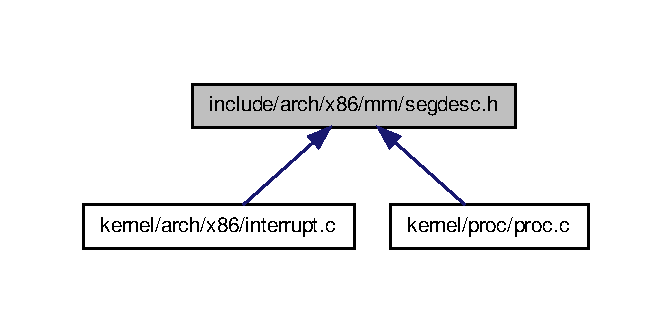
\includegraphics[width=322pt]{segdesc_8h__dep__incl}
\end{center}
\end{figure}
\subsection*{\-Defines}
\begin{DoxyCompactItemize}
\item 
\#define \hyperlink{segdesc_8h_a1c33e00098119b699555b4abfe41b70a}{\-S\-E\-G\-\_\-\-K\-E\-R\-N\-C\-O\-D\-E}~0x8
\item 
\#define \hyperlink{segdesc_8h_a0ba03ecd003750b615290460dfbb89a9}{\-S\-E\-G\-\_\-\-K\-E\-R\-N\-D\-A\-T\-A}~0x10
\item 
\#define \hyperlink{segdesc_8h_a869fe051e908e9b065451033e1202017}{\-S\-E\-G\-\_\-\-U\-S\-E\-R\-C\-O\-D\-E}~0x18
\item 
\#define \hyperlink{segdesc_8h_a2ae054259d69022f3a171f2e468dae54}{\-S\-E\-G\-\_\-\-U\-S\-E\-R\-D\-A\-T\-A}~0x20
\item 
\#define \hyperlink{segdesc_8h_a51332450caa8201ecc42fce428288e6f}{\-S\-E\-G\-\_\-\-T\-S\-S}~0x28
\end{DoxyCompactItemize}


\subsection{\-Define \-Documentation}
\hypertarget{segdesc_8h_a1c33e00098119b699555b4abfe41b70a}{\index{segdesc.\-h@{segdesc.\-h}!\-S\-E\-G\-\_\-\-K\-E\-R\-N\-C\-O\-D\-E@{\-S\-E\-G\-\_\-\-K\-E\-R\-N\-C\-O\-D\-E}}
\index{\-S\-E\-G\-\_\-\-K\-E\-R\-N\-C\-O\-D\-E@{\-S\-E\-G\-\_\-\-K\-E\-R\-N\-C\-O\-D\-E}!segdesc.h@{segdesc.\-h}}
\subsubsection[{\-S\-E\-G\-\_\-\-K\-E\-R\-N\-C\-O\-D\-E}]{\setlength{\rightskip}{0pt plus 5cm}\#define {\bf \-S\-E\-G\-\_\-\-K\-E\-R\-N\-C\-O\-D\-E}~0x8}}\label{segdesc_8h_a1c33e00098119b699555b4abfe41b70a}


\-Definition at line 8 of file segdesc.\-h.

\hypertarget{segdesc_8h_a0ba03ecd003750b615290460dfbb89a9}{\index{segdesc.\-h@{segdesc.\-h}!\-S\-E\-G\-\_\-\-K\-E\-R\-N\-D\-A\-T\-A@{\-S\-E\-G\-\_\-\-K\-E\-R\-N\-D\-A\-T\-A}}
\index{\-S\-E\-G\-\_\-\-K\-E\-R\-N\-D\-A\-T\-A@{\-S\-E\-G\-\_\-\-K\-E\-R\-N\-D\-A\-T\-A}!segdesc.h@{segdesc.\-h}}
\subsubsection[{\-S\-E\-G\-\_\-\-K\-E\-R\-N\-D\-A\-T\-A}]{\setlength{\rightskip}{0pt plus 5cm}\#define {\bf \-S\-E\-G\-\_\-\-K\-E\-R\-N\-D\-A\-T\-A}~0x10}}\label{segdesc_8h_a0ba03ecd003750b615290460dfbb89a9}


\-Definition at line 9 of file segdesc.\-h.

\hypertarget{segdesc_8h_a51332450caa8201ecc42fce428288e6f}{\index{segdesc.\-h@{segdesc.\-h}!\-S\-E\-G\-\_\-\-T\-S\-S@{\-S\-E\-G\-\_\-\-T\-S\-S}}
\index{\-S\-E\-G\-\_\-\-T\-S\-S@{\-S\-E\-G\-\_\-\-T\-S\-S}!segdesc.h@{segdesc.\-h}}
\subsubsection[{\-S\-E\-G\-\_\-\-T\-S\-S}]{\setlength{\rightskip}{0pt plus 5cm}\#define {\bf \-S\-E\-G\-\_\-\-T\-S\-S}~0x28}}\label{segdesc_8h_a51332450caa8201ecc42fce428288e6f}


\-Definition at line 12 of file segdesc.\-h.

\hypertarget{segdesc_8h_a869fe051e908e9b065451033e1202017}{\index{segdesc.\-h@{segdesc.\-h}!\-S\-E\-G\-\_\-\-U\-S\-E\-R\-C\-O\-D\-E@{\-S\-E\-G\-\_\-\-U\-S\-E\-R\-C\-O\-D\-E}}
\index{\-S\-E\-G\-\_\-\-U\-S\-E\-R\-C\-O\-D\-E@{\-S\-E\-G\-\_\-\-U\-S\-E\-R\-C\-O\-D\-E}!segdesc.h@{segdesc.\-h}}
\subsubsection[{\-S\-E\-G\-\_\-\-U\-S\-E\-R\-C\-O\-D\-E}]{\setlength{\rightskip}{0pt plus 5cm}\#define {\bf \-S\-E\-G\-\_\-\-U\-S\-E\-R\-C\-O\-D\-E}~0x18}}\label{segdesc_8h_a869fe051e908e9b065451033e1202017}


\-Definition at line 10 of file segdesc.\-h.

\hypertarget{segdesc_8h_a2ae054259d69022f3a171f2e468dae54}{\index{segdesc.\-h@{segdesc.\-h}!\-S\-E\-G\-\_\-\-U\-S\-E\-R\-D\-A\-T\-A@{\-S\-E\-G\-\_\-\-U\-S\-E\-R\-D\-A\-T\-A}}
\index{\-S\-E\-G\-\_\-\-U\-S\-E\-R\-D\-A\-T\-A@{\-S\-E\-G\-\_\-\-U\-S\-E\-R\-D\-A\-T\-A}!segdesc.h@{segdesc.\-h}}
\subsubsection[{\-S\-E\-G\-\_\-\-U\-S\-E\-R\-D\-A\-T\-A}]{\setlength{\rightskip}{0pt plus 5cm}\#define {\bf \-S\-E\-G\-\_\-\-U\-S\-E\-R\-D\-A\-T\-A}~0x20}}\label{segdesc_8h_a2ae054259d69022f3a171f2e468dae54}


\-Definition at line 11 of file segdesc.\-h.


\hypertarget{processor_8h}{\section{include/arch/x86/processor.h \-File \-Reference}
\label{processor_8h}\index{include/arch/x86/processor.\-h@{include/arch/x86/processor.\-h}}
}
\-This graph shows which files directly or indirectly include this file\-:\nopagebreak
\begin{figure}[H]
\begin{center}
\leavevmode
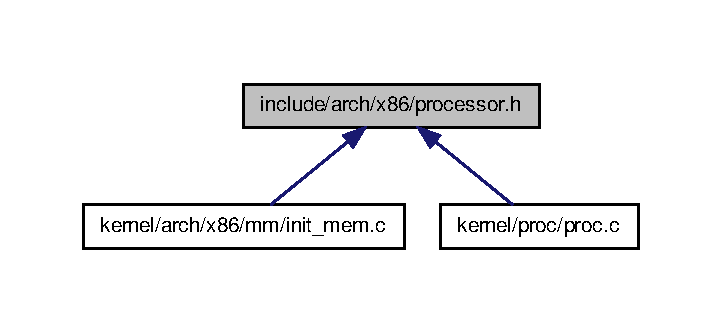
\includegraphics[width=346pt]{processor_8h__dep__incl}
\end{center}
\end{figure}
\subsection*{\-Defines}
\begin{DoxyCompactItemize}
\item 
\#define \hyperlink{processor_8h_a597ee77644c12219fb9ea52e20126522}{\-X86\-\_\-\-C\-R0\-\_\-\-P\-E}~0x00000001	/$\ast$ Protection Enable $\ast$/
\item 
\#define \hyperlink{processor_8h_a0d83e8761ecea0be4a9658e1bebab2bf}{\-X86\-\_\-\-C\-R0\-\_\-\-M\-P}~0x00000002	/$\ast$ Monitor Coprocessor $\ast$/
\item 
\#define \hyperlink{processor_8h_adf7d31c6132d58e480f50f31df4b5942}{\-X86\-\_\-\-C\-R0\-\_\-\-E\-M}~0x00000004	/$\ast$ Emulation $\ast$/
\item 
\#define \hyperlink{processor_8h_a9fc705998cbf68e9706a5149a755e832}{\-X86\-\_\-\-C\-R0\-\_\-\-T\-S}~0x00000008	/$\ast$ Task Switched $\ast$/
\item 
\#define \hyperlink{processor_8h_adbd34f1e859cc6b38101459d17e34701}{\-X86\-\_\-\-C\-R0\-\_\-\-E\-T}~0x00000010	/$\ast$ Extension type $\ast$/
\item 
\#define \hyperlink{processor_8h_a6871428c756277884dce3281af8358bf}{\-X86\-\_\-\-C\-R0\-\_\-\-N\-E}~0x00000020	/$\ast$ Numeric error $\ast$/
\item 
\#define \hyperlink{processor_8h_ad80f888ec507d366f5b8f0372ed1bc05}{\-X86\-\_\-\-C\-R0\-\_\-\-W\-P}~0x00010000	/$\ast$ Write Protect $\ast$/
\item 
\#define \hyperlink{processor_8h_a04ea804593f839c4ab2bc1feef760a73}{\-X86\-\_\-\-C\-R0\-\_\-\-A\-M}~0x00040000	/$\ast$ Alignment Mask $\ast$/
\item 
\#define \hyperlink{processor_8h_a869394d7cf13790e0214283c7e9f8194}{\-X86\-\_\-\-C\-R0\-\_\-\-N\-W}~0x20000000	/$\ast$ Not writable through $\ast$/
\item 
\#define \hyperlink{processor_8h_aebf661430d4577713142ff9f81a4d102}{\-X86\-\_\-\-C\-R0\-\_\-\-C\-D}~0x40000000	/$\ast$ Cache disabled $\ast$/
\item 
\#define \hyperlink{processor_8h_ab72deb63af2e514ee438b77ef1e84774}{\-X86\-\_\-\-C\-R0\-\_\-\-P\-G}~0x80000000	/$\ast$ Paging enable $\ast$/
\item 
\#define \hyperlink{processor_8h_a4119db930b70df9b5924616a8125ff84}{\-X86\-\_\-\-C\-R3\-\_\-\-P\-W\-T}~0x00000008	/$\ast$ Page Write Through $\ast$/
\item 
\#define \hyperlink{processor_8h_aab5dedf3133983fea452694efca8a1f1}{\-X86\-\_\-\-C\-R3\-\_\-\-P\-C\-D}~0x00000010	/$\ast$ Page Cache Disabled $\ast$/
\item 
\#define \hyperlink{processor_8h_a3222e39f032fc55acbccf8103653d1cf}{\-X86\-\_\-\-C\-R4\-\_\-\-V\-M\-E}~0x00000001	/$\ast$ Enable V\-M86 Extension $\ast$/
\item 
\#define \hyperlink{processor_8h_a41454d13f762adabb9a7ceb792c05b2d}{\-X86\-\_\-\-C\-R4\-\_\-\-P\-V\-I}~0x00000002	/$\ast$ Virtual interrupts flag enable $\ast$/
\item 
\#define \hyperlink{processor_8h_ab3ca2c2439512da0298be80aaa24d5bd}{\-X86\-\_\-\-C\-R4\-\_\-\-T\-S\-D}~0x00000004	/$\ast$ Disable time stamp at ipl 3 $\ast$/
\item 
\#define \hyperlink{processor_8h_ab30aed0358c581fc3bfbf6905d9881a9}{\-X86\-\_\-\-C\-R4\-\_\-\-D\-E}~0x00000008	/$\ast$ Enable Debugging extensions $\ast$/
\item 
\#define \hyperlink{processor_8h_a293066c70fa0a9de3b2e12368cb527ac}{\-X86\-\_\-\-C\-R4\-\_\-\-P\-S\-E}~0x00000010	/$\ast$ Enable Page Size extension $\ast$/
\item 
\#define \hyperlink{processor_8h_a0cb6a44b6c4f52eca15afeaa2b61e79e}{\-X86\-\_\-\-C\-R4\-\_\-\-P\-A\-E}~0x00000020	/$\ast$ Enable Physical address extension $\ast$/
\item 
\#define \hyperlink{processor_8h_af8ecc7a75011c464ce5bf0019d41fd8c}{\-X86\-\_\-\-C\-R4\-\_\-\-M\-C\-E}~0x00000040	/$\ast$ Machine Chech enable $\ast$/
\item 
\#define \hyperlink{processor_8h_ad23bda2721546baf492dad4af149fa71}{\-X86\-\_\-\-C\-R4\-\_\-\-P\-G\-E}~0x00000080	/$\ast$ Enable Global Pages $\ast$/
\item 
\#define \hyperlink{processor_8h_ae897ccbe936e5a72070061b44552db06}{\-X86\-\_\-\-C\-R4\-\_\-\-P\-C\-E}~0x00000100	/$\ast$ Enable Performance Counters at ipl 3$\ast$/
\item 
\#define \hyperlink{processor_8h_a6ba7f7e3e179f76fcf2608f271d1e651}{\-X86\-\_\-\-C\-R4\-\_\-\-O\-S\-F\-X\-S\-R}~0x00000200	/$\ast$ Enable Fast F\-P\-U save and restore $\ast$/
\item 
\#define \hyperlink{processor_8h_af0183ac7a7eb4f349f38006cae976796}{\-X86\-\_\-\-C\-R4\-\_\-\-O\-S\-X\-M\-M\-E\-X\-C\-P\-T}~0x00000400	/$\ast$ Enable unmasked S\-S\-E exceptions $\ast$/
\item 
\#define \hyperlink{processor_8h_a8352c2d920c1435e681c21a07c06b28c}{\-X86\-\_\-\-C\-R4\-\_\-\-V\-M\-X\-E}~0x00002000	/$\ast$ Enable V\-M\-X virtualization $\ast$/
\item 
\#define \hyperlink{processor_8h_acb4869a763bf0afca2fff1d44bcaf920}{\-X86\-\_\-\-C\-R4\-\_\-\-O\-S\-X\-S\-A\-V\-E}~0x00004000	/$\ast$ Enable Xsave and xrestore $\ast$/
\item 
\#define \hyperlink{processor_8h_a3962355b6f9b8842480d6c9842f4d609}{\-X86\-\_\-\-C\-R8\-\_\-\-T\-P\-R}~0x0000000\-F	/$\ast$ Task Priority Register $\ast$/
\item 
\#define \hyperlink{processor_8h_ab986e2506d41cc4c34ed200d4f1af152}{\-F\-L\-A\-G\-\_\-\-C\-F}~0x1
\item 
\#define \hyperlink{processor_8h_a9110b772ac704bd1274772a0cf1c7cd9}{\-F\-L\-A\-G\-\_\-\-P\-F}~0x4
\item 
\#define \hyperlink{processor_8h_a39b1b69d5d3c961e3cb3d29c6b07d566}{\-F\-L\-A\-G\-\_\-\-A\-F}~0x10
\item 
\#define \hyperlink{processor_8h_ad8903c2ead023ee8cd24695791d83d63}{\-F\-L\-A\-G\-\_\-\-Z\-F}~0x40
\item 
\#define \hyperlink{processor_8h_a46c416a4db6f14ff2e27c82844ac9b2a}{\-F\-L\-A\-G\-\_\-\-S\-F}~0x80
\item 
\#define \hyperlink{processor_8h_ae8932ec7b0ea0ddddf3262cedafc90c1}{\-F\-L\-A\-G\-\_\-\-T\-F}~0x100
\item 
\#define \hyperlink{processor_8h_a9ea36bf70e20601bdbefa9c7d7e0ad09}{\-F\-L\-A\-G\-\_\-\-I\-F}~0x200
\item 
\#define \hyperlink{processor_8h_a4c305ff02093002fffd78a460cc97544}{\-F\-L\-A\-G\-\_\-\-D\-F}~0x400
\item 
\#define \hyperlink{processor_8h_ab602d601b9d55752a3d1c57432bb78ca}{\-F\-L\-A\-G\-\_\-\-O\-F}~0x800
\item 
\#define \hyperlink{processor_8h_a562613e04f629238c17b69fee12d9ca9}{\-F\-L\-A\-G\-\_\-\-I\-O\-P\-L}~0x1000
\item 
\#define \hyperlink{processor_8h_afa1e13c0d70e6ce850d9781749af82f3}{\-F\-L\-A\-G\-\_\-\-N\-T}~0x2000
\item 
\#define \hyperlink{processor_8h_af3989e1484ca9ee0c8a68b466c3d233a}{\-F\-L\-A\-G\-\_\-\-R\-F}~0x4000
\item 
\#define \hyperlink{processor_8h_acfb792d06dfb29f9d8c9266bfaf1f172}{\-F\-L\-A\-G\-\_\-\-V\-M}~0x8000
\item 
\#define \hyperlink{processor_8h_ae7c594342e3f61c45e7db4ff74133827}{\-F\-L\-A\-G\-\_\-\-A\-C}~0x10000
\item 
\#define \hyperlink{processor_8h_aaa999059d2fc4368978776f8f328a9ed}{\-F\-L\-A\-G\-\_\-\-V\-I\-F}~0x20000
\item 
\#define \hyperlink{processor_8h_a005b6aaa02e4f1e8ea14a35986c24b65}{\-F\-L\-A\-G\-\_\-\-V\-I\-P}~0x40000
\item 
\#define \hyperlink{processor_8h_a5d3c13eae6153b442fbfe65bddfc33c7}{\-F\-L\-A\-G\-\_\-\-I\-D}~0x80000
\end{DoxyCompactItemize}


\subsection{\-Define \-Documentation}
\hypertarget{processor_8h_ae7c594342e3f61c45e7db4ff74133827}{\index{processor.\-h@{processor.\-h}!\-F\-L\-A\-G\-\_\-\-A\-C@{\-F\-L\-A\-G\-\_\-\-A\-C}}
\index{\-F\-L\-A\-G\-\_\-\-A\-C@{\-F\-L\-A\-G\-\_\-\-A\-C}!processor.h@{processor.\-h}}
\subsubsection[{\-F\-L\-A\-G\-\_\-\-A\-C}]{\setlength{\rightskip}{0pt plus 5cm}\#define {\bf \-F\-L\-A\-G\-\_\-\-A\-C}~0x10000}}\label{processor_8h_ae7c594342e3f61c45e7db4ff74133827}


\-Definition at line 54 of file processor.\-h.

\hypertarget{processor_8h_a39b1b69d5d3c961e3cb3d29c6b07d566}{\index{processor.\-h@{processor.\-h}!\-F\-L\-A\-G\-\_\-\-A\-F@{\-F\-L\-A\-G\-\_\-\-A\-F}}
\index{\-F\-L\-A\-G\-\_\-\-A\-F@{\-F\-L\-A\-G\-\_\-\-A\-F}!processor.h@{processor.\-h}}
\subsubsection[{\-F\-L\-A\-G\-\_\-\-A\-F}]{\setlength{\rightskip}{0pt plus 5cm}\#define {\bf \-F\-L\-A\-G\-\_\-\-A\-F}~0x10}}\label{processor_8h_a39b1b69d5d3c961e3cb3d29c6b07d566}


\-Definition at line 43 of file processor.\-h.

\hypertarget{processor_8h_ab986e2506d41cc4c34ed200d4f1af152}{\index{processor.\-h@{processor.\-h}!\-F\-L\-A\-G\-\_\-\-C\-F@{\-F\-L\-A\-G\-\_\-\-C\-F}}
\index{\-F\-L\-A\-G\-\_\-\-C\-F@{\-F\-L\-A\-G\-\_\-\-C\-F}!processor.h@{processor.\-h}}
\subsubsection[{\-F\-L\-A\-G\-\_\-\-C\-F}]{\setlength{\rightskip}{0pt plus 5cm}\#define {\bf \-F\-L\-A\-G\-\_\-\-C\-F}~0x1}}\label{processor_8h_ab986e2506d41cc4c34ed200d4f1af152}


\-Definition at line 41 of file processor.\-h.

\hypertarget{processor_8h_a4c305ff02093002fffd78a460cc97544}{\index{processor.\-h@{processor.\-h}!\-F\-L\-A\-G\-\_\-\-D\-F@{\-F\-L\-A\-G\-\_\-\-D\-F}}
\index{\-F\-L\-A\-G\-\_\-\-D\-F@{\-F\-L\-A\-G\-\_\-\-D\-F}!processor.h@{processor.\-h}}
\subsubsection[{\-F\-L\-A\-G\-\_\-\-D\-F}]{\setlength{\rightskip}{0pt plus 5cm}\#define {\bf \-F\-L\-A\-G\-\_\-\-D\-F}~0x400}}\label{processor_8h_a4c305ff02093002fffd78a460cc97544}


\-Definition at line 48 of file processor.\-h.

\hypertarget{processor_8h_a5d3c13eae6153b442fbfe65bddfc33c7}{\index{processor.\-h@{processor.\-h}!\-F\-L\-A\-G\-\_\-\-I\-D@{\-F\-L\-A\-G\-\_\-\-I\-D}}
\index{\-F\-L\-A\-G\-\_\-\-I\-D@{\-F\-L\-A\-G\-\_\-\-I\-D}!processor.h@{processor.\-h}}
\subsubsection[{\-F\-L\-A\-G\-\_\-\-I\-D}]{\setlength{\rightskip}{0pt plus 5cm}\#define {\bf \-F\-L\-A\-G\-\_\-\-I\-D}~0x80000}}\label{processor_8h_a5d3c13eae6153b442fbfe65bddfc33c7}


\-Definition at line 57 of file processor.\-h.

\hypertarget{processor_8h_a9ea36bf70e20601bdbefa9c7d7e0ad09}{\index{processor.\-h@{processor.\-h}!\-F\-L\-A\-G\-\_\-\-I\-F@{\-F\-L\-A\-G\-\_\-\-I\-F}}
\index{\-F\-L\-A\-G\-\_\-\-I\-F@{\-F\-L\-A\-G\-\_\-\-I\-F}!processor.h@{processor.\-h}}
\subsubsection[{\-F\-L\-A\-G\-\_\-\-I\-F}]{\setlength{\rightskip}{0pt plus 5cm}\#define {\bf \-F\-L\-A\-G\-\_\-\-I\-F}~0x200}}\label{processor_8h_a9ea36bf70e20601bdbefa9c7d7e0ad09}


\-Definition at line 47 of file processor.\-h.

\hypertarget{processor_8h_a562613e04f629238c17b69fee12d9ca9}{\index{processor.\-h@{processor.\-h}!\-F\-L\-A\-G\-\_\-\-I\-O\-P\-L@{\-F\-L\-A\-G\-\_\-\-I\-O\-P\-L}}
\index{\-F\-L\-A\-G\-\_\-\-I\-O\-P\-L@{\-F\-L\-A\-G\-\_\-\-I\-O\-P\-L}!processor.h@{processor.\-h}}
\subsubsection[{\-F\-L\-A\-G\-\_\-\-I\-O\-P\-L}]{\setlength{\rightskip}{0pt plus 5cm}\#define {\bf \-F\-L\-A\-G\-\_\-\-I\-O\-P\-L}~0x1000}}\label{processor_8h_a562613e04f629238c17b69fee12d9ca9}


\-Definition at line 50 of file processor.\-h.

\hypertarget{processor_8h_afa1e13c0d70e6ce850d9781749af82f3}{\index{processor.\-h@{processor.\-h}!\-F\-L\-A\-G\-\_\-\-N\-T@{\-F\-L\-A\-G\-\_\-\-N\-T}}
\index{\-F\-L\-A\-G\-\_\-\-N\-T@{\-F\-L\-A\-G\-\_\-\-N\-T}!processor.h@{processor.\-h}}
\subsubsection[{\-F\-L\-A\-G\-\_\-\-N\-T}]{\setlength{\rightskip}{0pt plus 5cm}\#define {\bf \-F\-L\-A\-G\-\_\-\-N\-T}~0x2000}}\label{processor_8h_afa1e13c0d70e6ce850d9781749af82f3}


\-Definition at line 51 of file processor.\-h.

\hypertarget{processor_8h_ab602d601b9d55752a3d1c57432bb78ca}{\index{processor.\-h@{processor.\-h}!\-F\-L\-A\-G\-\_\-\-O\-F@{\-F\-L\-A\-G\-\_\-\-O\-F}}
\index{\-F\-L\-A\-G\-\_\-\-O\-F@{\-F\-L\-A\-G\-\_\-\-O\-F}!processor.h@{processor.\-h}}
\subsubsection[{\-F\-L\-A\-G\-\_\-\-O\-F}]{\setlength{\rightskip}{0pt plus 5cm}\#define {\bf \-F\-L\-A\-G\-\_\-\-O\-F}~0x800}}\label{processor_8h_ab602d601b9d55752a3d1c57432bb78ca}


\-Definition at line 49 of file processor.\-h.

\hypertarget{processor_8h_a9110b772ac704bd1274772a0cf1c7cd9}{\index{processor.\-h@{processor.\-h}!\-F\-L\-A\-G\-\_\-\-P\-F@{\-F\-L\-A\-G\-\_\-\-P\-F}}
\index{\-F\-L\-A\-G\-\_\-\-P\-F@{\-F\-L\-A\-G\-\_\-\-P\-F}!processor.h@{processor.\-h}}
\subsubsection[{\-F\-L\-A\-G\-\_\-\-P\-F}]{\setlength{\rightskip}{0pt plus 5cm}\#define {\bf \-F\-L\-A\-G\-\_\-\-P\-F}~0x4}}\label{processor_8h_a9110b772ac704bd1274772a0cf1c7cd9}


\-Definition at line 42 of file processor.\-h.

\hypertarget{processor_8h_af3989e1484ca9ee0c8a68b466c3d233a}{\index{processor.\-h@{processor.\-h}!\-F\-L\-A\-G\-\_\-\-R\-F@{\-F\-L\-A\-G\-\_\-\-R\-F}}
\index{\-F\-L\-A\-G\-\_\-\-R\-F@{\-F\-L\-A\-G\-\_\-\-R\-F}!processor.h@{processor.\-h}}
\subsubsection[{\-F\-L\-A\-G\-\_\-\-R\-F}]{\setlength{\rightskip}{0pt plus 5cm}\#define {\bf \-F\-L\-A\-G\-\_\-\-R\-F}~0x4000}}\label{processor_8h_af3989e1484ca9ee0c8a68b466c3d233a}


\-Definition at line 52 of file processor.\-h.

\hypertarget{processor_8h_a46c416a4db6f14ff2e27c82844ac9b2a}{\index{processor.\-h@{processor.\-h}!\-F\-L\-A\-G\-\_\-\-S\-F@{\-F\-L\-A\-G\-\_\-\-S\-F}}
\index{\-F\-L\-A\-G\-\_\-\-S\-F@{\-F\-L\-A\-G\-\_\-\-S\-F}!processor.h@{processor.\-h}}
\subsubsection[{\-F\-L\-A\-G\-\_\-\-S\-F}]{\setlength{\rightskip}{0pt plus 5cm}\#define {\bf \-F\-L\-A\-G\-\_\-\-S\-F}~0x80}}\label{processor_8h_a46c416a4db6f14ff2e27c82844ac9b2a}


\-Definition at line 45 of file processor.\-h.

\hypertarget{processor_8h_ae8932ec7b0ea0ddddf3262cedafc90c1}{\index{processor.\-h@{processor.\-h}!\-F\-L\-A\-G\-\_\-\-T\-F@{\-F\-L\-A\-G\-\_\-\-T\-F}}
\index{\-F\-L\-A\-G\-\_\-\-T\-F@{\-F\-L\-A\-G\-\_\-\-T\-F}!processor.h@{processor.\-h}}
\subsubsection[{\-F\-L\-A\-G\-\_\-\-T\-F}]{\setlength{\rightskip}{0pt plus 5cm}\#define {\bf \-F\-L\-A\-G\-\_\-\-T\-F}~0x100}}\label{processor_8h_ae8932ec7b0ea0ddddf3262cedafc90c1}


\-Definition at line 46 of file processor.\-h.

\hypertarget{processor_8h_aaa999059d2fc4368978776f8f328a9ed}{\index{processor.\-h@{processor.\-h}!\-F\-L\-A\-G\-\_\-\-V\-I\-F@{\-F\-L\-A\-G\-\_\-\-V\-I\-F}}
\index{\-F\-L\-A\-G\-\_\-\-V\-I\-F@{\-F\-L\-A\-G\-\_\-\-V\-I\-F}!processor.h@{processor.\-h}}
\subsubsection[{\-F\-L\-A\-G\-\_\-\-V\-I\-F}]{\setlength{\rightskip}{0pt plus 5cm}\#define {\bf \-F\-L\-A\-G\-\_\-\-V\-I\-F}~0x20000}}\label{processor_8h_aaa999059d2fc4368978776f8f328a9ed}


\-Definition at line 55 of file processor.\-h.

\hypertarget{processor_8h_a005b6aaa02e4f1e8ea14a35986c24b65}{\index{processor.\-h@{processor.\-h}!\-F\-L\-A\-G\-\_\-\-V\-I\-P@{\-F\-L\-A\-G\-\_\-\-V\-I\-P}}
\index{\-F\-L\-A\-G\-\_\-\-V\-I\-P@{\-F\-L\-A\-G\-\_\-\-V\-I\-P}!processor.h@{processor.\-h}}
\subsubsection[{\-F\-L\-A\-G\-\_\-\-V\-I\-P}]{\setlength{\rightskip}{0pt plus 5cm}\#define {\bf \-F\-L\-A\-G\-\_\-\-V\-I\-P}~0x40000}}\label{processor_8h_a005b6aaa02e4f1e8ea14a35986c24b65}


\-Definition at line 56 of file processor.\-h.

\hypertarget{processor_8h_acfb792d06dfb29f9d8c9266bfaf1f172}{\index{processor.\-h@{processor.\-h}!\-F\-L\-A\-G\-\_\-\-V\-M@{\-F\-L\-A\-G\-\_\-\-V\-M}}
\index{\-F\-L\-A\-G\-\_\-\-V\-M@{\-F\-L\-A\-G\-\_\-\-V\-M}!processor.h@{processor.\-h}}
\subsubsection[{\-F\-L\-A\-G\-\_\-\-V\-M}]{\setlength{\rightskip}{0pt plus 5cm}\#define {\bf \-F\-L\-A\-G\-\_\-\-V\-M}~0x8000}}\label{processor_8h_acfb792d06dfb29f9d8c9266bfaf1f172}


\-Definition at line 53 of file processor.\-h.

\hypertarget{processor_8h_ad8903c2ead023ee8cd24695791d83d63}{\index{processor.\-h@{processor.\-h}!\-F\-L\-A\-G\-\_\-\-Z\-F@{\-F\-L\-A\-G\-\_\-\-Z\-F}}
\index{\-F\-L\-A\-G\-\_\-\-Z\-F@{\-F\-L\-A\-G\-\_\-\-Z\-F}!processor.h@{processor.\-h}}
\subsubsection[{\-F\-L\-A\-G\-\_\-\-Z\-F}]{\setlength{\rightskip}{0pt plus 5cm}\#define {\bf \-F\-L\-A\-G\-\_\-\-Z\-F}~0x40}}\label{processor_8h_ad8903c2ead023ee8cd24695791d83d63}


\-Definition at line 44 of file processor.\-h.

\hypertarget{processor_8h_a04ea804593f839c4ab2bc1feef760a73}{\index{processor.\-h@{processor.\-h}!\-X86\-\_\-\-C\-R0\-\_\-\-A\-M@{\-X86\-\_\-\-C\-R0\-\_\-\-A\-M}}
\index{\-X86\-\_\-\-C\-R0\-\_\-\-A\-M@{\-X86\-\_\-\-C\-R0\-\_\-\-A\-M}!processor.h@{processor.\-h}}
\subsubsection[{\-X86\-\_\-\-C\-R0\-\_\-\-A\-M}]{\setlength{\rightskip}{0pt plus 5cm}\#define {\bf \-X86\-\_\-\-C\-R0\-\_\-\-A\-M}~0x00040000	/$\ast$ Alignment Mask $\ast$/}}\label{processor_8h_a04ea804593f839c4ab2bc1feef760a73}


\-Definition at line 12 of file processor.\-h.

\hypertarget{processor_8h_aebf661430d4577713142ff9f81a4d102}{\index{processor.\-h@{processor.\-h}!\-X86\-\_\-\-C\-R0\-\_\-\-C\-D@{\-X86\-\_\-\-C\-R0\-\_\-\-C\-D}}
\index{\-X86\-\_\-\-C\-R0\-\_\-\-C\-D@{\-X86\-\_\-\-C\-R0\-\_\-\-C\-D}!processor.h@{processor.\-h}}
\subsubsection[{\-X86\-\_\-\-C\-R0\-\_\-\-C\-D}]{\setlength{\rightskip}{0pt plus 5cm}\#define {\bf \-X86\-\_\-\-C\-R0\-\_\-\-C\-D}~0x40000000	/$\ast$ Cache disabled $\ast$/}}\label{processor_8h_aebf661430d4577713142ff9f81a4d102}


\-Definition at line 14 of file processor.\-h.

\hypertarget{processor_8h_adf7d31c6132d58e480f50f31df4b5942}{\index{processor.\-h@{processor.\-h}!\-X86\-\_\-\-C\-R0\-\_\-\-E\-M@{\-X86\-\_\-\-C\-R0\-\_\-\-E\-M}}
\index{\-X86\-\_\-\-C\-R0\-\_\-\-E\-M@{\-X86\-\_\-\-C\-R0\-\_\-\-E\-M}!processor.h@{processor.\-h}}
\subsubsection[{\-X86\-\_\-\-C\-R0\-\_\-\-E\-M}]{\setlength{\rightskip}{0pt plus 5cm}\#define {\bf \-X86\-\_\-\-C\-R0\-\_\-\-E\-M}~0x00000004	/$\ast$ Emulation $\ast$/}}\label{processor_8h_adf7d31c6132d58e480f50f31df4b5942}


\-Definition at line 7 of file processor.\-h.

\hypertarget{processor_8h_adbd34f1e859cc6b38101459d17e34701}{\index{processor.\-h@{processor.\-h}!\-X86\-\_\-\-C\-R0\-\_\-\-E\-T@{\-X86\-\_\-\-C\-R0\-\_\-\-E\-T}}
\index{\-X86\-\_\-\-C\-R0\-\_\-\-E\-T@{\-X86\-\_\-\-C\-R0\-\_\-\-E\-T}!processor.h@{processor.\-h}}
\subsubsection[{\-X86\-\_\-\-C\-R0\-\_\-\-E\-T}]{\setlength{\rightskip}{0pt plus 5cm}\#define {\bf \-X86\-\_\-\-C\-R0\-\_\-\-E\-T}~0x00000010	/$\ast$ Extension type $\ast$/}}\label{processor_8h_adbd34f1e859cc6b38101459d17e34701}


\-Definition at line 9 of file processor.\-h.

\hypertarget{processor_8h_a0d83e8761ecea0be4a9658e1bebab2bf}{\index{processor.\-h@{processor.\-h}!\-X86\-\_\-\-C\-R0\-\_\-\-M\-P@{\-X86\-\_\-\-C\-R0\-\_\-\-M\-P}}
\index{\-X86\-\_\-\-C\-R0\-\_\-\-M\-P@{\-X86\-\_\-\-C\-R0\-\_\-\-M\-P}!processor.h@{processor.\-h}}
\subsubsection[{\-X86\-\_\-\-C\-R0\-\_\-\-M\-P}]{\setlength{\rightskip}{0pt plus 5cm}\#define {\bf \-X86\-\_\-\-C\-R0\-\_\-\-M\-P}~0x00000002	/$\ast$ Monitor Coprocessor $\ast$/}}\label{processor_8h_a0d83e8761ecea0be4a9658e1bebab2bf}


\-Definition at line 6 of file processor.\-h.

\hypertarget{processor_8h_a6871428c756277884dce3281af8358bf}{\index{processor.\-h@{processor.\-h}!\-X86\-\_\-\-C\-R0\-\_\-\-N\-E@{\-X86\-\_\-\-C\-R0\-\_\-\-N\-E}}
\index{\-X86\-\_\-\-C\-R0\-\_\-\-N\-E@{\-X86\-\_\-\-C\-R0\-\_\-\-N\-E}!processor.h@{processor.\-h}}
\subsubsection[{\-X86\-\_\-\-C\-R0\-\_\-\-N\-E}]{\setlength{\rightskip}{0pt plus 5cm}\#define {\bf \-X86\-\_\-\-C\-R0\-\_\-\-N\-E}~0x00000020	/$\ast$ Numeric error $\ast$/}}\label{processor_8h_a6871428c756277884dce3281af8358bf}


\-Definition at line 10 of file processor.\-h.

\hypertarget{processor_8h_a869394d7cf13790e0214283c7e9f8194}{\index{processor.\-h@{processor.\-h}!\-X86\-\_\-\-C\-R0\-\_\-\-N\-W@{\-X86\-\_\-\-C\-R0\-\_\-\-N\-W}}
\index{\-X86\-\_\-\-C\-R0\-\_\-\-N\-W@{\-X86\-\_\-\-C\-R0\-\_\-\-N\-W}!processor.h@{processor.\-h}}
\subsubsection[{\-X86\-\_\-\-C\-R0\-\_\-\-N\-W}]{\setlength{\rightskip}{0pt plus 5cm}\#define {\bf \-X86\-\_\-\-C\-R0\-\_\-\-N\-W}~0x20000000	/$\ast$ Not writable through $\ast$/}}\label{processor_8h_a869394d7cf13790e0214283c7e9f8194}


\-Definition at line 13 of file processor.\-h.

\hypertarget{processor_8h_a597ee77644c12219fb9ea52e20126522}{\index{processor.\-h@{processor.\-h}!\-X86\-\_\-\-C\-R0\-\_\-\-P\-E@{\-X86\-\_\-\-C\-R0\-\_\-\-P\-E}}
\index{\-X86\-\_\-\-C\-R0\-\_\-\-P\-E@{\-X86\-\_\-\-C\-R0\-\_\-\-P\-E}!processor.h@{processor.\-h}}
\subsubsection[{\-X86\-\_\-\-C\-R0\-\_\-\-P\-E}]{\setlength{\rightskip}{0pt plus 5cm}\#define {\bf \-X86\-\_\-\-C\-R0\-\_\-\-P\-E}~0x00000001	/$\ast$ Protection Enable $\ast$/}}\label{processor_8h_a597ee77644c12219fb9ea52e20126522}


\-Definition at line 5 of file processor.\-h.

\hypertarget{processor_8h_ab72deb63af2e514ee438b77ef1e84774}{\index{processor.\-h@{processor.\-h}!\-X86\-\_\-\-C\-R0\-\_\-\-P\-G@{\-X86\-\_\-\-C\-R0\-\_\-\-P\-G}}
\index{\-X86\-\_\-\-C\-R0\-\_\-\-P\-G@{\-X86\-\_\-\-C\-R0\-\_\-\-P\-G}!processor.h@{processor.\-h}}
\subsubsection[{\-X86\-\_\-\-C\-R0\-\_\-\-P\-G}]{\setlength{\rightskip}{0pt plus 5cm}\#define {\bf \-X86\-\_\-\-C\-R0\-\_\-\-P\-G}~0x80000000	/$\ast$ Paging enable $\ast$/}}\label{processor_8h_ab72deb63af2e514ee438b77ef1e84774}


\-Definition at line 15 of file processor.\-h.

\hypertarget{processor_8h_a9fc705998cbf68e9706a5149a755e832}{\index{processor.\-h@{processor.\-h}!\-X86\-\_\-\-C\-R0\-\_\-\-T\-S@{\-X86\-\_\-\-C\-R0\-\_\-\-T\-S}}
\index{\-X86\-\_\-\-C\-R0\-\_\-\-T\-S@{\-X86\-\_\-\-C\-R0\-\_\-\-T\-S}!processor.h@{processor.\-h}}
\subsubsection[{\-X86\-\_\-\-C\-R0\-\_\-\-T\-S}]{\setlength{\rightskip}{0pt plus 5cm}\#define {\bf \-X86\-\_\-\-C\-R0\-\_\-\-T\-S}~0x00000008	/$\ast$ Task Switched $\ast$/}}\label{processor_8h_a9fc705998cbf68e9706a5149a755e832}


\-Definition at line 8 of file processor.\-h.

\hypertarget{processor_8h_ad80f888ec507d366f5b8f0372ed1bc05}{\index{processor.\-h@{processor.\-h}!\-X86\-\_\-\-C\-R0\-\_\-\-W\-P@{\-X86\-\_\-\-C\-R0\-\_\-\-W\-P}}
\index{\-X86\-\_\-\-C\-R0\-\_\-\-W\-P@{\-X86\-\_\-\-C\-R0\-\_\-\-W\-P}!processor.h@{processor.\-h}}
\subsubsection[{\-X86\-\_\-\-C\-R0\-\_\-\-W\-P}]{\setlength{\rightskip}{0pt plus 5cm}\#define {\bf \-X86\-\_\-\-C\-R0\-\_\-\-W\-P}~0x00010000	/$\ast$ Write Protect $\ast$/}}\label{processor_8h_ad80f888ec507d366f5b8f0372ed1bc05}


\-Definition at line 11 of file processor.\-h.

\hypertarget{processor_8h_aab5dedf3133983fea452694efca8a1f1}{\index{processor.\-h@{processor.\-h}!\-X86\-\_\-\-C\-R3\-\_\-\-P\-C\-D@{\-X86\-\_\-\-C\-R3\-\_\-\-P\-C\-D}}
\index{\-X86\-\_\-\-C\-R3\-\_\-\-P\-C\-D@{\-X86\-\_\-\-C\-R3\-\_\-\-P\-C\-D}!processor.h@{processor.\-h}}
\subsubsection[{\-X86\-\_\-\-C\-R3\-\_\-\-P\-C\-D}]{\setlength{\rightskip}{0pt plus 5cm}\#define {\bf \-X86\-\_\-\-C\-R3\-\_\-\-P\-C\-D}~0x00000010	/$\ast$ Page Cache Disabled $\ast$/}}\label{processor_8h_aab5dedf3133983fea452694efca8a1f1}


\-Definition at line 19 of file processor.\-h.

\hypertarget{processor_8h_a4119db930b70df9b5924616a8125ff84}{\index{processor.\-h@{processor.\-h}!\-X86\-\_\-\-C\-R3\-\_\-\-P\-W\-T@{\-X86\-\_\-\-C\-R3\-\_\-\-P\-W\-T}}
\index{\-X86\-\_\-\-C\-R3\-\_\-\-P\-W\-T@{\-X86\-\_\-\-C\-R3\-\_\-\-P\-W\-T}!processor.h@{processor.\-h}}
\subsubsection[{\-X86\-\_\-\-C\-R3\-\_\-\-P\-W\-T}]{\setlength{\rightskip}{0pt plus 5cm}\#define {\bf \-X86\-\_\-\-C\-R3\-\_\-\-P\-W\-T}~0x00000008	/$\ast$ Page Write Through $\ast$/}}\label{processor_8h_a4119db930b70df9b5924616a8125ff84}


\-Definition at line 18 of file processor.\-h.

\hypertarget{processor_8h_ab30aed0358c581fc3bfbf6905d9881a9}{\index{processor.\-h@{processor.\-h}!\-X86\-\_\-\-C\-R4\-\_\-\-D\-E@{\-X86\-\_\-\-C\-R4\-\_\-\-D\-E}}
\index{\-X86\-\_\-\-C\-R4\-\_\-\-D\-E@{\-X86\-\_\-\-C\-R4\-\_\-\-D\-E}!processor.h@{processor.\-h}}
\subsubsection[{\-X86\-\_\-\-C\-R4\-\_\-\-D\-E}]{\setlength{\rightskip}{0pt plus 5cm}\#define {\bf \-X86\-\_\-\-C\-R4\-\_\-\-D\-E}~0x00000008	/$\ast$ Enable Debugging extensions $\ast$/}}\label{processor_8h_ab30aed0358c581fc3bfbf6905d9881a9}


\-Definition at line 25 of file processor.\-h.

\hypertarget{processor_8h_af8ecc7a75011c464ce5bf0019d41fd8c}{\index{processor.\-h@{processor.\-h}!\-X86\-\_\-\-C\-R4\-\_\-\-M\-C\-E@{\-X86\-\_\-\-C\-R4\-\_\-\-M\-C\-E}}
\index{\-X86\-\_\-\-C\-R4\-\_\-\-M\-C\-E@{\-X86\-\_\-\-C\-R4\-\_\-\-M\-C\-E}!processor.h@{processor.\-h}}
\subsubsection[{\-X86\-\_\-\-C\-R4\-\_\-\-M\-C\-E}]{\setlength{\rightskip}{0pt plus 5cm}\#define {\bf \-X86\-\_\-\-C\-R4\-\_\-\-M\-C\-E}~0x00000040	/$\ast$ Machine Chech enable $\ast$/}}\label{processor_8h_af8ecc7a75011c464ce5bf0019d41fd8c}


\-Definition at line 28 of file processor.\-h.

\hypertarget{processor_8h_a6ba7f7e3e179f76fcf2608f271d1e651}{\index{processor.\-h@{processor.\-h}!\-X86\-\_\-\-C\-R4\-\_\-\-O\-S\-F\-X\-S\-R@{\-X86\-\_\-\-C\-R4\-\_\-\-O\-S\-F\-X\-S\-R}}
\index{\-X86\-\_\-\-C\-R4\-\_\-\-O\-S\-F\-X\-S\-R@{\-X86\-\_\-\-C\-R4\-\_\-\-O\-S\-F\-X\-S\-R}!processor.h@{processor.\-h}}
\subsubsection[{\-X86\-\_\-\-C\-R4\-\_\-\-O\-S\-F\-X\-S\-R}]{\setlength{\rightskip}{0pt plus 5cm}\#define {\bf \-X86\-\_\-\-C\-R4\-\_\-\-O\-S\-F\-X\-S\-R}~0x00000200	/$\ast$ Enable Fast F\-P\-U save and restore $\ast$/}}\label{processor_8h_a6ba7f7e3e179f76fcf2608f271d1e651}


\-Definition at line 31 of file processor.\-h.

\hypertarget{processor_8h_af0183ac7a7eb4f349f38006cae976796}{\index{processor.\-h@{processor.\-h}!\-X86\-\_\-\-C\-R4\-\_\-\-O\-S\-X\-M\-M\-E\-X\-C\-P\-T@{\-X86\-\_\-\-C\-R4\-\_\-\-O\-S\-X\-M\-M\-E\-X\-C\-P\-T}}
\index{\-X86\-\_\-\-C\-R4\-\_\-\-O\-S\-X\-M\-M\-E\-X\-C\-P\-T@{\-X86\-\_\-\-C\-R4\-\_\-\-O\-S\-X\-M\-M\-E\-X\-C\-P\-T}!processor.h@{processor.\-h}}
\subsubsection[{\-X86\-\_\-\-C\-R4\-\_\-\-O\-S\-X\-M\-M\-E\-X\-C\-P\-T}]{\setlength{\rightskip}{0pt plus 5cm}\#define {\bf \-X86\-\_\-\-C\-R4\-\_\-\-O\-S\-X\-M\-M\-E\-X\-C\-P\-T}~0x00000400	/$\ast$ Enable unmasked S\-S\-E exceptions $\ast$/}}\label{processor_8h_af0183ac7a7eb4f349f38006cae976796}


\-Definition at line 32 of file processor.\-h.

\hypertarget{processor_8h_acb4869a763bf0afca2fff1d44bcaf920}{\index{processor.\-h@{processor.\-h}!\-X86\-\_\-\-C\-R4\-\_\-\-O\-S\-X\-S\-A\-V\-E@{\-X86\-\_\-\-C\-R4\-\_\-\-O\-S\-X\-S\-A\-V\-E}}
\index{\-X86\-\_\-\-C\-R4\-\_\-\-O\-S\-X\-S\-A\-V\-E@{\-X86\-\_\-\-C\-R4\-\_\-\-O\-S\-X\-S\-A\-V\-E}!processor.h@{processor.\-h}}
\subsubsection[{\-X86\-\_\-\-C\-R4\-\_\-\-O\-S\-X\-S\-A\-V\-E}]{\setlength{\rightskip}{0pt plus 5cm}\#define {\bf \-X86\-\_\-\-C\-R4\-\_\-\-O\-S\-X\-S\-A\-V\-E}~0x00004000	/$\ast$ Enable Xsave and xrestore $\ast$/}}\label{processor_8h_acb4869a763bf0afca2fff1d44bcaf920}


\-Definition at line 34 of file processor.\-h.

\hypertarget{processor_8h_a0cb6a44b6c4f52eca15afeaa2b61e79e}{\index{processor.\-h@{processor.\-h}!\-X86\-\_\-\-C\-R4\-\_\-\-P\-A\-E@{\-X86\-\_\-\-C\-R4\-\_\-\-P\-A\-E}}
\index{\-X86\-\_\-\-C\-R4\-\_\-\-P\-A\-E@{\-X86\-\_\-\-C\-R4\-\_\-\-P\-A\-E}!processor.h@{processor.\-h}}
\subsubsection[{\-X86\-\_\-\-C\-R4\-\_\-\-P\-A\-E}]{\setlength{\rightskip}{0pt plus 5cm}\#define {\bf \-X86\-\_\-\-C\-R4\-\_\-\-P\-A\-E}~0x00000020	/$\ast$ Enable Physical address extension $\ast$/}}\label{processor_8h_a0cb6a44b6c4f52eca15afeaa2b61e79e}


\-Definition at line 27 of file processor.\-h.

\hypertarget{processor_8h_ae897ccbe936e5a72070061b44552db06}{\index{processor.\-h@{processor.\-h}!\-X86\-\_\-\-C\-R4\-\_\-\-P\-C\-E@{\-X86\-\_\-\-C\-R4\-\_\-\-P\-C\-E}}
\index{\-X86\-\_\-\-C\-R4\-\_\-\-P\-C\-E@{\-X86\-\_\-\-C\-R4\-\_\-\-P\-C\-E}!processor.h@{processor.\-h}}
\subsubsection[{\-X86\-\_\-\-C\-R4\-\_\-\-P\-C\-E}]{\setlength{\rightskip}{0pt plus 5cm}\#define {\bf \-X86\-\_\-\-C\-R4\-\_\-\-P\-C\-E}~0x00000100	/$\ast$ Enable Performance Counters at ipl 3$\ast$/}}\label{processor_8h_ae897ccbe936e5a72070061b44552db06}


\-Definition at line 30 of file processor.\-h.

\hypertarget{processor_8h_ad23bda2721546baf492dad4af149fa71}{\index{processor.\-h@{processor.\-h}!\-X86\-\_\-\-C\-R4\-\_\-\-P\-G\-E@{\-X86\-\_\-\-C\-R4\-\_\-\-P\-G\-E}}
\index{\-X86\-\_\-\-C\-R4\-\_\-\-P\-G\-E@{\-X86\-\_\-\-C\-R4\-\_\-\-P\-G\-E}!processor.h@{processor.\-h}}
\subsubsection[{\-X86\-\_\-\-C\-R4\-\_\-\-P\-G\-E}]{\setlength{\rightskip}{0pt plus 5cm}\#define {\bf \-X86\-\_\-\-C\-R4\-\_\-\-P\-G\-E}~0x00000080	/$\ast$ Enable Global Pages $\ast$/}}\label{processor_8h_ad23bda2721546baf492dad4af149fa71}


\-Definition at line 29 of file processor.\-h.

\hypertarget{processor_8h_a293066c70fa0a9de3b2e12368cb527ac}{\index{processor.\-h@{processor.\-h}!\-X86\-\_\-\-C\-R4\-\_\-\-P\-S\-E@{\-X86\-\_\-\-C\-R4\-\_\-\-P\-S\-E}}
\index{\-X86\-\_\-\-C\-R4\-\_\-\-P\-S\-E@{\-X86\-\_\-\-C\-R4\-\_\-\-P\-S\-E}!processor.h@{processor.\-h}}
\subsubsection[{\-X86\-\_\-\-C\-R4\-\_\-\-P\-S\-E}]{\setlength{\rightskip}{0pt plus 5cm}\#define {\bf \-X86\-\_\-\-C\-R4\-\_\-\-P\-S\-E}~0x00000010	/$\ast$ Enable Page Size extension $\ast$/}}\label{processor_8h_a293066c70fa0a9de3b2e12368cb527ac}


\-Definition at line 26 of file processor.\-h.

\hypertarget{processor_8h_a41454d13f762adabb9a7ceb792c05b2d}{\index{processor.\-h@{processor.\-h}!\-X86\-\_\-\-C\-R4\-\_\-\-P\-V\-I@{\-X86\-\_\-\-C\-R4\-\_\-\-P\-V\-I}}
\index{\-X86\-\_\-\-C\-R4\-\_\-\-P\-V\-I@{\-X86\-\_\-\-C\-R4\-\_\-\-P\-V\-I}!processor.h@{processor.\-h}}
\subsubsection[{\-X86\-\_\-\-C\-R4\-\_\-\-P\-V\-I}]{\setlength{\rightskip}{0pt plus 5cm}\#define {\bf \-X86\-\_\-\-C\-R4\-\_\-\-P\-V\-I}~0x00000002	/$\ast$ Virtual interrupts flag enable $\ast$/}}\label{processor_8h_a41454d13f762adabb9a7ceb792c05b2d}


\-Definition at line 23 of file processor.\-h.

\hypertarget{processor_8h_ab3ca2c2439512da0298be80aaa24d5bd}{\index{processor.\-h@{processor.\-h}!\-X86\-\_\-\-C\-R4\-\_\-\-T\-S\-D@{\-X86\-\_\-\-C\-R4\-\_\-\-T\-S\-D}}
\index{\-X86\-\_\-\-C\-R4\-\_\-\-T\-S\-D@{\-X86\-\_\-\-C\-R4\-\_\-\-T\-S\-D}!processor.h@{processor.\-h}}
\subsubsection[{\-X86\-\_\-\-C\-R4\-\_\-\-T\-S\-D}]{\setlength{\rightskip}{0pt plus 5cm}\#define {\bf \-X86\-\_\-\-C\-R4\-\_\-\-T\-S\-D}~0x00000004	/$\ast$ Disable time stamp at ipl 3 $\ast$/}}\label{processor_8h_ab3ca2c2439512da0298be80aaa24d5bd}


\-Definition at line 24 of file processor.\-h.

\hypertarget{processor_8h_a3222e39f032fc55acbccf8103653d1cf}{\index{processor.\-h@{processor.\-h}!\-X86\-\_\-\-C\-R4\-\_\-\-V\-M\-E@{\-X86\-\_\-\-C\-R4\-\_\-\-V\-M\-E}}
\index{\-X86\-\_\-\-C\-R4\-\_\-\-V\-M\-E@{\-X86\-\_\-\-C\-R4\-\_\-\-V\-M\-E}!processor.h@{processor.\-h}}
\subsubsection[{\-X86\-\_\-\-C\-R4\-\_\-\-V\-M\-E}]{\setlength{\rightskip}{0pt plus 5cm}\#define {\bf \-X86\-\_\-\-C\-R4\-\_\-\-V\-M\-E}~0x00000001	/$\ast$ Enable V\-M86 Extension $\ast$/}}\label{processor_8h_a3222e39f032fc55acbccf8103653d1cf}


\-Definition at line 22 of file processor.\-h.

\hypertarget{processor_8h_a8352c2d920c1435e681c21a07c06b28c}{\index{processor.\-h@{processor.\-h}!\-X86\-\_\-\-C\-R4\-\_\-\-V\-M\-X\-E@{\-X86\-\_\-\-C\-R4\-\_\-\-V\-M\-X\-E}}
\index{\-X86\-\_\-\-C\-R4\-\_\-\-V\-M\-X\-E@{\-X86\-\_\-\-C\-R4\-\_\-\-V\-M\-X\-E}!processor.h@{processor.\-h}}
\subsubsection[{\-X86\-\_\-\-C\-R4\-\_\-\-V\-M\-X\-E}]{\setlength{\rightskip}{0pt plus 5cm}\#define {\bf \-X86\-\_\-\-C\-R4\-\_\-\-V\-M\-X\-E}~0x00002000	/$\ast$ Enable V\-M\-X virtualization $\ast$/}}\label{processor_8h_a8352c2d920c1435e681c21a07c06b28c}


\-Definition at line 33 of file processor.\-h.

\hypertarget{processor_8h_a3962355b6f9b8842480d6c9842f4d609}{\index{processor.\-h@{processor.\-h}!\-X86\-\_\-\-C\-R8\-\_\-\-T\-P\-R@{\-X86\-\_\-\-C\-R8\-\_\-\-T\-P\-R}}
\index{\-X86\-\_\-\-C\-R8\-\_\-\-T\-P\-R@{\-X86\-\_\-\-C\-R8\-\_\-\-T\-P\-R}!processor.h@{processor.\-h}}
\subsubsection[{\-X86\-\_\-\-C\-R8\-\_\-\-T\-P\-R}]{\setlength{\rightskip}{0pt plus 5cm}\#define {\bf \-X86\-\_\-\-C\-R8\-\_\-\-T\-P\-R}~0x0000000\-F	/$\ast$ Task Priority Register $\ast$/}}\label{processor_8h_a3962355b6f9b8842480d6c9842f4d609}


\-Definition at line 37 of file processor.\-h.


\hypertarget{vectors_8h}{\section{include/arch/x86/vectors.h \-File \-Reference}
\label{vectors_8h}\index{include/arch/x86/vectors.\-h@{include/arch/x86/vectors.\-h}}
}
\-This graph shows which files directly or indirectly include this file\-:\nopagebreak
\begin{figure}[H]
\begin{center}
\leavevmode
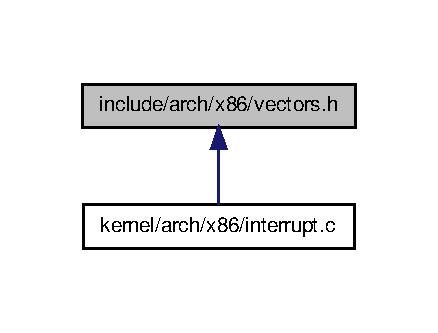
\includegraphics[width=210pt]{vectors_8h__dep__incl}
\end{center}
\end{figure}
\subsection*{\-Variables}
\begin{DoxyCompactItemize}
\item 
\hyperlink{types_8h_a435d1572bf3f880d55459d9805097f62}{uint32\-\_\-t} \hyperlink{vectors_8h_a1ac2619f785b484f5b60c3b1f9cb3387}{vector\-\_\-0}
\item 
\hyperlink{types_8h_a435d1572bf3f880d55459d9805097f62}{uint32\-\_\-t} \hyperlink{vectors_8h_a4d707440b7821089b6b54ee7bf0ff0b5}{vector\-\_\-1}
\item 
\hyperlink{types_8h_a435d1572bf3f880d55459d9805097f62}{uint32\-\_\-t} \hyperlink{vectors_8h_a36f7e4c448c60e892ed97ac9e865c203}{vector\-\_\-2}
\item 
\hyperlink{types_8h_a435d1572bf3f880d55459d9805097f62}{uint32\-\_\-t} \hyperlink{vectors_8h_a7b5fd2eab87eb413f433a7ea7e256461}{vector\-\_\-3}
\item 
\hyperlink{types_8h_a435d1572bf3f880d55459d9805097f62}{uint32\-\_\-t} \hyperlink{vectors_8h_a2a51ed177f7f7c5376517c809d79dbe4}{vector\-\_\-4}
\item 
\hyperlink{types_8h_a435d1572bf3f880d55459d9805097f62}{uint32\-\_\-t} \hyperlink{vectors_8h_a54c12cfc4bdd9e40cac435d4cd0fdba4}{vector\-\_\-5}
\item 
\hyperlink{types_8h_a435d1572bf3f880d55459d9805097f62}{uint32\-\_\-t} \hyperlink{vectors_8h_a674c09aebcc291346519d8575f63d699}{vector\-\_\-6}
\item 
\hyperlink{types_8h_a435d1572bf3f880d55459d9805097f62}{uint32\-\_\-t} \hyperlink{vectors_8h_a166cbc136a407ae63289353f41847367}{vector\-\_\-7}
\item 
\hyperlink{types_8h_a435d1572bf3f880d55459d9805097f62}{uint32\-\_\-t} \hyperlink{vectors_8h_a7b113b125c0cd7c618f6a96704961fed}{vector\-\_\-8}
\item 
\hyperlink{types_8h_a435d1572bf3f880d55459d9805097f62}{uint32\-\_\-t} \hyperlink{vectors_8h_afce34cc2691df6b8a18920242904f2ca}{vector\-\_\-9}
\item 
\hyperlink{types_8h_a435d1572bf3f880d55459d9805097f62}{uint32\-\_\-t} \hyperlink{vectors_8h_a363bcf87f1d6a89e5f7c3205fa650613}{vector\-\_\-10}
\item 
\hyperlink{types_8h_a435d1572bf3f880d55459d9805097f62}{uint32\-\_\-t} \hyperlink{vectors_8h_a182396c735d6950e7e339164bcc504ea}{vector\-\_\-11}
\item 
\hyperlink{types_8h_a435d1572bf3f880d55459d9805097f62}{uint32\-\_\-t} \hyperlink{vectors_8h_a22fc19d59a3f97a7324b978a34230b10}{vector\-\_\-12}
\item 
\hyperlink{types_8h_a435d1572bf3f880d55459d9805097f62}{uint32\-\_\-t} \hyperlink{vectors_8h_a00aa01300886286373e4501c3c2f30d9}{vector\-\_\-13}
\item 
\hyperlink{types_8h_a435d1572bf3f880d55459d9805097f62}{uint32\-\_\-t} \hyperlink{vectors_8h_ac0f24dcbd603d275fcf806fbfff6ae36}{vector\-\_\-14}
\item 
\hyperlink{types_8h_a435d1572bf3f880d55459d9805097f62}{uint32\-\_\-t} \hyperlink{vectors_8h_aa286f2de56d799719948bd49f59c5e68}{vector\-\_\-15}
\item 
\hyperlink{types_8h_a435d1572bf3f880d55459d9805097f62}{uint32\-\_\-t} \hyperlink{vectors_8h_a46e517a4aac8e430a76a444b7a76c88d}{vector\-\_\-16}
\item 
\hyperlink{types_8h_a435d1572bf3f880d55459d9805097f62}{uint32\-\_\-t} \hyperlink{vectors_8h_ad1567b893cbc9175444f1b5fd7e322ba}{vector\-\_\-17}
\item 
\hyperlink{types_8h_a435d1572bf3f880d55459d9805097f62}{uint32\-\_\-t} \hyperlink{vectors_8h_adc2dc58bf4ee2a8e64673d3daedf88d9}{vector\-\_\-18}
\item 
\hyperlink{types_8h_a435d1572bf3f880d55459d9805097f62}{uint32\-\_\-t} \hyperlink{vectors_8h_aff92ee2aedcd51aaeacd74bd1fbf92ed}{vector\-\_\-19}
\item 
\hyperlink{types_8h_a435d1572bf3f880d55459d9805097f62}{uint32\-\_\-t} \hyperlink{vectors_8h_ad7e73ba4f893a2f6421f81ba53bd0d26}{vector\-\_\-20}
\item 
\hyperlink{types_8h_a435d1572bf3f880d55459d9805097f62}{uint32\-\_\-t} \hyperlink{vectors_8h_a961a672277fdfcbc5ea51c87b350f2e4}{vector\-\_\-21}
\item 
\hyperlink{types_8h_a435d1572bf3f880d55459d9805097f62}{uint32\-\_\-t} \hyperlink{vectors_8h_aaa6758e613985a0b19d5db2d43c9cd65}{vector\-\_\-22}
\item 
\hyperlink{types_8h_a435d1572bf3f880d55459d9805097f62}{uint32\-\_\-t} \hyperlink{vectors_8h_a58a1fe492760c4439fb622668cc7fdba}{vector\-\_\-23}
\item 
\hyperlink{types_8h_a435d1572bf3f880d55459d9805097f62}{uint32\-\_\-t} \hyperlink{vectors_8h_a2aa20ef437349aa539f84aa569cc1766}{vector\-\_\-24}
\item 
\hyperlink{types_8h_a435d1572bf3f880d55459d9805097f62}{uint32\-\_\-t} \hyperlink{vectors_8h_af470485705a8f32d34b37577cadd7878}{vector\-\_\-25}
\item 
\hyperlink{types_8h_a435d1572bf3f880d55459d9805097f62}{uint32\-\_\-t} \hyperlink{vectors_8h_ad1a68b6231c8ac321a4376a96670fa1b}{vector\-\_\-26}
\item 
\hyperlink{types_8h_a435d1572bf3f880d55459d9805097f62}{uint32\-\_\-t} \hyperlink{vectors_8h_adf3e0128922ccce8f568e94488d63933}{vector\-\_\-27}
\item 
\hyperlink{types_8h_a435d1572bf3f880d55459d9805097f62}{uint32\-\_\-t} \hyperlink{vectors_8h_a0f7a2386162d48ef0ef3f1cc87cdd286}{vector\-\_\-28}
\item 
\hyperlink{types_8h_a435d1572bf3f880d55459d9805097f62}{uint32\-\_\-t} \hyperlink{vectors_8h_a501f8b7ef72d271c90d30817a2880832}{vector\-\_\-29}
\item 
\hyperlink{types_8h_a435d1572bf3f880d55459d9805097f62}{uint32\-\_\-t} \hyperlink{vectors_8h_acce0e4e7f67e01c6ee6f11b194ce50c0}{vector\-\_\-30}
\item 
\hyperlink{types_8h_a435d1572bf3f880d55459d9805097f62}{uint32\-\_\-t} \hyperlink{vectors_8h_a26b0c58ae44cd2dc0f38c31ab78f571c}{vector\-\_\-31}
\item 
\hyperlink{types_8h_a435d1572bf3f880d55459d9805097f62}{uint32\-\_\-t} \hyperlink{vectors_8h_a1a6d8b9feacb5ef53b959f39b382b40f}{vector\-\_\-32}
\item 
\hyperlink{types_8h_a435d1572bf3f880d55459d9805097f62}{uint32\-\_\-t} \hyperlink{vectors_8h_a23a084134b6c4903e2cab461f80285e3}{vector\-\_\-33}
\item 
\hyperlink{types_8h_a435d1572bf3f880d55459d9805097f62}{uint32\-\_\-t} \hyperlink{vectors_8h_ac7f701a9b0ca9327c7c34b5808c71a62}{vector\-\_\-34}
\item 
\hyperlink{types_8h_a435d1572bf3f880d55459d9805097f62}{uint32\-\_\-t} \hyperlink{vectors_8h_a0aeceefa6c8475a2b3aeb4b36437fa86}{vector\-\_\-35}
\item 
\hyperlink{types_8h_a435d1572bf3f880d55459d9805097f62}{uint32\-\_\-t} \hyperlink{vectors_8h_aece1255b0c9590dbcc8357aed3597cc9}{vector\-\_\-36}
\item 
\hyperlink{types_8h_a435d1572bf3f880d55459d9805097f62}{uint32\-\_\-t} \hyperlink{vectors_8h_a5b1b0709250bbc152e13912b4bfda3f5}{vector\-\_\-37}
\item 
\hyperlink{types_8h_a435d1572bf3f880d55459d9805097f62}{uint32\-\_\-t} \hyperlink{vectors_8h_accb1c3c22972e22ed41bd0755fe529b8}{vector\-\_\-38}
\item 
\hyperlink{types_8h_a435d1572bf3f880d55459d9805097f62}{uint32\-\_\-t} \hyperlink{vectors_8h_a0cfb661282efeafe7256ab79f7ac1238}{vector\-\_\-39}
\item 
\hyperlink{types_8h_a435d1572bf3f880d55459d9805097f62}{uint32\-\_\-t} \hyperlink{vectors_8h_a802d2e238fa9e86e961ee9ca355c7338}{vector\-\_\-40}
\item 
\hyperlink{types_8h_a435d1572bf3f880d55459d9805097f62}{uint32\-\_\-t} \hyperlink{vectors_8h_a3bd338603b3399a2a296c687dc463294}{vector\-\_\-41}
\item 
\hyperlink{types_8h_a435d1572bf3f880d55459d9805097f62}{uint32\-\_\-t} \hyperlink{vectors_8h_a7e3d4bb1ef50576a2c1bb2204ce2249d}{vector\-\_\-42}
\item 
\hyperlink{types_8h_a435d1572bf3f880d55459d9805097f62}{uint32\-\_\-t} \hyperlink{vectors_8h_a8055746602ab9e1f52675705bd687015}{vector\-\_\-43}
\item 
\hyperlink{types_8h_a435d1572bf3f880d55459d9805097f62}{uint32\-\_\-t} \hyperlink{vectors_8h_a1ec3db1ff0f61834785439c0b4abb378}{vector\-\_\-44}
\item 
\hyperlink{types_8h_a435d1572bf3f880d55459d9805097f62}{uint32\-\_\-t} \hyperlink{vectors_8h_a1f5d7e5ddc1848a4710f9e587eea782b}{vector\-\_\-45}
\item 
\hyperlink{types_8h_a435d1572bf3f880d55459d9805097f62}{uint32\-\_\-t} \hyperlink{vectors_8h_af33505977b22de784c2a0ab072dc258d}{vector\-\_\-46}
\item 
\hyperlink{types_8h_a435d1572bf3f880d55459d9805097f62}{uint32\-\_\-t} \hyperlink{vectors_8h_a08fd740f928a96d6f926f34d5dbcc847}{vector\-\_\-47}
\item 
\hyperlink{types_8h_a435d1572bf3f880d55459d9805097f62}{uint32\-\_\-t} \hyperlink{vectors_8h_a60b94b396f8841dfb8168ec879875287}{vector\-\_\-48}
\item 
\hyperlink{types_8h_a435d1572bf3f880d55459d9805097f62}{uint32\-\_\-t} \hyperlink{vectors_8h_a12bd9cf9d2ba637bc0f4d4f1653d1838}{vector\-\_\-49}
\item 
\hyperlink{types_8h_a435d1572bf3f880d55459d9805097f62}{uint32\-\_\-t} \hyperlink{vectors_8h_aef930d47188e79a1a58d515e1e4bbd7f}{vector\-\_\-50}
\item 
\hyperlink{types_8h_a435d1572bf3f880d55459d9805097f62}{uint32\-\_\-t} \hyperlink{vectors_8h_a068982c9918a211e61ac9bc67ec00169}{vector\-\_\-51}
\item 
\hyperlink{types_8h_a435d1572bf3f880d55459d9805097f62}{uint32\-\_\-t} \hyperlink{vectors_8h_a13146ddadf7527f2127f0d7596f667ae}{vector\-\_\-52}
\item 
\hyperlink{types_8h_a435d1572bf3f880d55459d9805097f62}{uint32\-\_\-t} \hyperlink{vectors_8h_a1513e4e39da9008f6d440c0a969cb85b}{vector\-\_\-53}
\item 
\hyperlink{types_8h_a435d1572bf3f880d55459d9805097f62}{uint32\-\_\-t} \hyperlink{vectors_8h_a2d56cc05ee30ad75d3c91c1281b138ae}{vector\-\_\-54}
\item 
\hyperlink{types_8h_a435d1572bf3f880d55459d9805097f62}{uint32\-\_\-t} \hyperlink{vectors_8h_a27e674d616bd077514bac9117940a214}{vector\-\_\-55}
\item 
\hyperlink{types_8h_a435d1572bf3f880d55459d9805097f62}{uint32\-\_\-t} \hyperlink{vectors_8h_a08859aaadbad3d22ced84adbf3d94ef4}{vector\-\_\-56}
\item 
\hyperlink{types_8h_a435d1572bf3f880d55459d9805097f62}{uint32\-\_\-t} \hyperlink{vectors_8h_a9137b0844d0691c54c2238bc55fc3dc1}{vector\-\_\-57}
\item 
\hyperlink{types_8h_a435d1572bf3f880d55459d9805097f62}{uint32\-\_\-t} \hyperlink{vectors_8h_ab4b2a43046927caf481dc212ae180014}{vector\-\_\-58}
\item 
\hyperlink{types_8h_a435d1572bf3f880d55459d9805097f62}{uint32\-\_\-t} \hyperlink{vectors_8h_ac08efc6c7a00ad96634a90c4515debe7}{vector\-\_\-59}
\item 
\hyperlink{types_8h_a435d1572bf3f880d55459d9805097f62}{uint32\-\_\-t} \hyperlink{vectors_8h_aa005b3e609b26e19f87bdb7c289de73f}{vector\-\_\-60}
\item 
\hyperlink{types_8h_a435d1572bf3f880d55459d9805097f62}{uint32\-\_\-t} \hyperlink{vectors_8h_a4551b070c5f593b252a81e3e497923e3}{vector\-\_\-61}
\item 
\hyperlink{types_8h_a435d1572bf3f880d55459d9805097f62}{uint32\-\_\-t} \hyperlink{vectors_8h_a49b25d94b52b3bdb6bc2460a9ee24243}{vector\-\_\-62}
\item 
\hyperlink{types_8h_a435d1572bf3f880d55459d9805097f62}{uint32\-\_\-t} \hyperlink{vectors_8h_afde0d83ab48d3a940e152b535083181a}{vector\-\_\-63}
\end{DoxyCompactItemize}


\subsection{\-Variable \-Documentation}
\hypertarget{vectors_8h_a1ac2619f785b484f5b60c3b1f9cb3387}{\index{vectors.\-h@{vectors.\-h}!vector\-\_\-0@{vector\-\_\-0}}
\index{vector\-\_\-0@{vector\-\_\-0}!vectors.h@{vectors.\-h}}
\subsubsection[{vector\-\_\-0}]{\setlength{\rightskip}{0pt plus 5cm}{\bf uint32\-\_\-t} {\bf vector\-\_\-0}}}\label{vectors_8h_a1ac2619f785b484f5b60c3b1f9cb3387}
\hypertarget{vectors_8h_a4d707440b7821089b6b54ee7bf0ff0b5}{\index{vectors.\-h@{vectors.\-h}!vector\-\_\-1@{vector\-\_\-1}}
\index{vector\-\_\-1@{vector\-\_\-1}!vectors.h@{vectors.\-h}}
\subsubsection[{vector\-\_\-1}]{\setlength{\rightskip}{0pt plus 5cm}{\bf uint32\-\_\-t} {\bf vector\-\_\-1}}}\label{vectors_8h_a4d707440b7821089b6b54ee7bf0ff0b5}
\hypertarget{vectors_8h_a363bcf87f1d6a89e5f7c3205fa650613}{\index{vectors.\-h@{vectors.\-h}!vector\-\_\-10@{vector\-\_\-10}}
\index{vector\-\_\-10@{vector\-\_\-10}!vectors.h@{vectors.\-h}}
\subsubsection[{vector\-\_\-10}]{\setlength{\rightskip}{0pt plus 5cm}{\bf uint32\-\_\-t} {\bf vector\-\_\-10}}}\label{vectors_8h_a363bcf87f1d6a89e5f7c3205fa650613}
\hypertarget{vectors_8h_a182396c735d6950e7e339164bcc504ea}{\index{vectors.\-h@{vectors.\-h}!vector\-\_\-11@{vector\-\_\-11}}
\index{vector\-\_\-11@{vector\-\_\-11}!vectors.h@{vectors.\-h}}
\subsubsection[{vector\-\_\-11}]{\setlength{\rightskip}{0pt plus 5cm}{\bf uint32\-\_\-t} {\bf vector\-\_\-11}}}\label{vectors_8h_a182396c735d6950e7e339164bcc504ea}
\hypertarget{vectors_8h_a22fc19d59a3f97a7324b978a34230b10}{\index{vectors.\-h@{vectors.\-h}!vector\-\_\-12@{vector\-\_\-12}}
\index{vector\-\_\-12@{vector\-\_\-12}!vectors.h@{vectors.\-h}}
\subsubsection[{vector\-\_\-12}]{\setlength{\rightskip}{0pt plus 5cm}{\bf uint32\-\_\-t} {\bf vector\-\_\-12}}}\label{vectors_8h_a22fc19d59a3f97a7324b978a34230b10}
\hypertarget{vectors_8h_a00aa01300886286373e4501c3c2f30d9}{\index{vectors.\-h@{vectors.\-h}!vector\-\_\-13@{vector\-\_\-13}}
\index{vector\-\_\-13@{vector\-\_\-13}!vectors.h@{vectors.\-h}}
\subsubsection[{vector\-\_\-13}]{\setlength{\rightskip}{0pt plus 5cm}{\bf uint32\-\_\-t} {\bf vector\-\_\-13}}}\label{vectors_8h_a00aa01300886286373e4501c3c2f30d9}
\hypertarget{vectors_8h_ac0f24dcbd603d275fcf806fbfff6ae36}{\index{vectors.\-h@{vectors.\-h}!vector\-\_\-14@{vector\-\_\-14}}
\index{vector\-\_\-14@{vector\-\_\-14}!vectors.h@{vectors.\-h}}
\subsubsection[{vector\-\_\-14}]{\setlength{\rightskip}{0pt plus 5cm}{\bf uint32\-\_\-t} {\bf vector\-\_\-14}}}\label{vectors_8h_ac0f24dcbd603d275fcf806fbfff6ae36}
\hypertarget{vectors_8h_aa286f2de56d799719948bd49f59c5e68}{\index{vectors.\-h@{vectors.\-h}!vector\-\_\-15@{vector\-\_\-15}}
\index{vector\-\_\-15@{vector\-\_\-15}!vectors.h@{vectors.\-h}}
\subsubsection[{vector\-\_\-15}]{\setlength{\rightskip}{0pt plus 5cm}{\bf uint32\-\_\-t} {\bf vector\-\_\-15}}}\label{vectors_8h_aa286f2de56d799719948bd49f59c5e68}
\hypertarget{vectors_8h_a46e517a4aac8e430a76a444b7a76c88d}{\index{vectors.\-h@{vectors.\-h}!vector\-\_\-16@{vector\-\_\-16}}
\index{vector\-\_\-16@{vector\-\_\-16}!vectors.h@{vectors.\-h}}
\subsubsection[{vector\-\_\-16}]{\setlength{\rightskip}{0pt plus 5cm}{\bf uint32\-\_\-t} {\bf vector\-\_\-16}}}\label{vectors_8h_a46e517a4aac8e430a76a444b7a76c88d}
\hypertarget{vectors_8h_ad1567b893cbc9175444f1b5fd7e322ba}{\index{vectors.\-h@{vectors.\-h}!vector\-\_\-17@{vector\-\_\-17}}
\index{vector\-\_\-17@{vector\-\_\-17}!vectors.h@{vectors.\-h}}
\subsubsection[{vector\-\_\-17}]{\setlength{\rightskip}{0pt plus 5cm}{\bf uint32\-\_\-t} {\bf vector\-\_\-17}}}\label{vectors_8h_ad1567b893cbc9175444f1b5fd7e322ba}
\hypertarget{vectors_8h_adc2dc58bf4ee2a8e64673d3daedf88d9}{\index{vectors.\-h@{vectors.\-h}!vector\-\_\-18@{vector\-\_\-18}}
\index{vector\-\_\-18@{vector\-\_\-18}!vectors.h@{vectors.\-h}}
\subsubsection[{vector\-\_\-18}]{\setlength{\rightskip}{0pt plus 5cm}{\bf uint32\-\_\-t} {\bf vector\-\_\-18}}}\label{vectors_8h_adc2dc58bf4ee2a8e64673d3daedf88d9}
\hypertarget{vectors_8h_aff92ee2aedcd51aaeacd74bd1fbf92ed}{\index{vectors.\-h@{vectors.\-h}!vector\-\_\-19@{vector\-\_\-19}}
\index{vector\-\_\-19@{vector\-\_\-19}!vectors.h@{vectors.\-h}}
\subsubsection[{vector\-\_\-19}]{\setlength{\rightskip}{0pt plus 5cm}{\bf uint32\-\_\-t} {\bf vector\-\_\-19}}}\label{vectors_8h_aff92ee2aedcd51aaeacd74bd1fbf92ed}
\hypertarget{vectors_8h_a36f7e4c448c60e892ed97ac9e865c203}{\index{vectors.\-h@{vectors.\-h}!vector\-\_\-2@{vector\-\_\-2}}
\index{vector\-\_\-2@{vector\-\_\-2}!vectors.h@{vectors.\-h}}
\subsubsection[{vector\-\_\-2}]{\setlength{\rightskip}{0pt plus 5cm}{\bf uint32\-\_\-t} {\bf vector\-\_\-2}}}\label{vectors_8h_a36f7e4c448c60e892ed97ac9e865c203}
\hypertarget{vectors_8h_ad7e73ba4f893a2f6421f81ba53bd0d26}{\index{vectors.\-h@{vectors.\-h}!vector\-\_\-20@{vector\-\_\-20}}
\index{vector\-\_\-20@{vector\-\_\-20}!vectors.h@{vectors.\-h}}
\subsubsection[{vector\-\_\-20}]{\setlength{\rightskip}{0pt plus 5cm}{\bf uint32\-\_\-t} {\bf vector\-\_\-20}}}\label{vectors_8h_ad7e73ba4f893a2f6421f81ba53bd0d26}
\hypertarget{vectors_8h_a961a672277fdfcbc5ea51c87b350f2e4}{\index{vectors.\-h@{vectors.\-h}!vector\-\_\-21@{vector\-\_\-21}}
\index{vector\-\_\-21@{vector\-\_\-21}!vectors.h@{vectors.\-h}}
\subsubsection[{vector\-\_\-21}]{\setlength{\rightskip}{0pt plus 5cm}{\bf uint32\-\_\-t} {\bf vector\-\_\-21}}}\label{vectors_8h_a961a672277fdfcbc5ea51c87b350f2e4}
\hypertarget{vectors_8h_aaa6758e613985a0b19d5db2d43c9cd65}{\index{vectors.\-h@{vectors.\-h}!vector\-\_\-22@{vector\-\_\-22}}
\index{vector\-\_\-22@{vector\-\_\-22}!vectors.h@{vectors.\-h}}
\subsubsection[{vector\-\_\-22}]{\setlength{\rightskip}{0pt plus 5cm}{\bf uint32\-\_\-t} {\bf vector\-\_\-22}}}\label{vectors_8h_aaa6758e613985a0b19d5db2d43c9cd65}
\hypertarget{vectors_8h_a58a1fe492760c4439fb622668cc7fdba}{\index{vectors.\-h@{vectors.\-h}!vector\-\_\-23@{vector\-\_\-23}}
\index{vector\-\_\-23@{vector\-\_\-23}!vectors.h@{vectors.\-h}}
\subsubsection[{vector\-\_\-23}]{\setlength{\rightskip}{0pt plus 5cm}{\bf uint32\-\_\-t} {\bf vector\-\_\-23}}}\label{vectors_8h_a58a1fe492760c4439fb622668cc7fdba}
\hypertarget{vectors_8h_a2aa20ef437349aa539f84aa569cc1766}{\index{vectors.\-h@{vectors.\-h}!vector\-\_\-24@{vector\-\_\-24}}
\index{vector\-\_\-24@{vector\-\_\-24}!vectors.h@{vectors.\-h}}
\subsubsection[{vector\-\_\-24}]{\setlength{\rightskip}{0pt plus 5cm}{\bf uint32\-\_\-t} {\bf vector\-\_\-24}}}\label{vectors_8h_a2aa20ef437349aa539f84aa569cc1766}
\hypertarget{vectors_8h_af470485705a8f32d34b37577cadd7878}{\index{vectors.\-h@{vectors.\-h}!vector\-\_\-25@{vector\-\_\-25}}
\index{vector\-\_\-25@{vector\-\_\-25}!vectors.h@{vectors.\-h}}
\subsubsection[{vector\-\_\-25}]{\setlength{\rightskip}{0pt plus 5cm}{\bf uint32\-\_\-t} {\bf vector\-\_\-25}}}\label{vectors_8h_af470485705a8f32d34b37577cadd7878}
\hypertarget{vectors_8h_ad1a68b6231c8ac321a4376a96670fa1b}{\index{vectors.\-h@{vectors.\-h}!vector\-\_\-26@{vector\-\_\-26}}
\index{vector\-\_\-26@{vector\-\_\-26}!vectors.h@{vectors.\-h}}
\subsubsection[{vector\-\_\-26}]{\setlength{\rightskip}{0pt plus 5cm}{\bf uint32\-\_\-t} {\bf vector\-\_\-26}}}\label{vectors_8h_ad1a68b6231c8ac321a4376a96670fa1b}
\hypertarget{vectors_8h_adf3e0128922ccce8f568e94488d63933}{\index{vectors.\-h@{vectors.\-h}!vector\-\_\-27@{vector\-\_\-27}}
\index{vector\-\_\-27@{vector\-\_\-27}!vectors.h@{vectors.\-h}}
\subsubsection[{vector\-\_\-27}]{\setlength{\rightskip}{0pt plus 5cm}{\bf uint32\-\_\-t} {\bf vector\-\_\-27}}}\label{vectors_8h_adf3e0128922ccce8f568e94488d63933}
\hypertarget{vectors_8h_a0f7a2386162d48ef0ef3f1cc87cdd286}{\index{vectors.\-h@{vectors.\-h}!vector\-\_\-28@{vector\-\_\-28}}
\index{vector\-\_\-28@{vector\-\_\-28}!vectors.h@{vectors.\-h}}
\subsubsection[{vector\-\_\-28}]{\setlength{\rightskip}{0pt plus 5cm}{\bf uint32\-\_\-t} {\bf vector\-\_\-28}}}\label{vectors_8h_a0f7a2386162d48ef0ef3f1cc87cdd286}
\hypertarget{vectors_8h_a501f8b7ef72d271c90d30817a2880832}{\index{vectors.\-h@{vectors.\-h}!vector\-\_\-29@{vector\-\_\-29}}
\index{vector\-\_\-29@{vector\-\_\-29}!vectors.h@{vectors.\-h}}
\subsubsection[{vector\-\_\-29}]{\setlength{\rightskip}{0pt plus 5cm}{\bf uint32\-\_\-t} {\bf vector\-\_\-29}}}\label{vectors_8h_a501f8b7ef72d271c90d30817a2880832}
\hypertarget{vectors_8h_a7b5fd2eab87eb413f433a7ea7e256461}{\index{vectors.\-h@{vectors.\-h}!vector\-\_\-3@{vector\-\_\-3}}
\index{vector\-\_\-3@{vector\-\_\-3}!vectors.h@{vectors.\-h}}
\subsubsection[{vector\-\_\-3}]{\setlength{\rightskip}{0pt plus 5cm}{\bf uint32\-\_\-t} {\bf vector\-\_\-3}}}\label{vectors_8h_a7b5fd2eab87eb413f433a7ea7e256461}
\hypertarget{vectors_8h_acce0e4e7f67e01c6ee6f11b194ce50c0}{\index{vectors.\-h@{vectors.\-h}!vector\-\_\-30@{vector\-\_\-30}}
\index{vector\-\_\-30@{vector\-\_\-30}!vectors.h@{vectors.\-h}}
\subsubsection[{vector\-\_\-30}]{\setlength{\rightskip}{0pt plus 5cm}{\bf uint32\-\_\-t} {\bf vector\-\_\-30}}}\label{vectors_8h_acce0e4e7f67e01c6ee6f11b194ce50c0}
\hypertarget{vectors_8h_a26b0c58ae44cd2dc0f38c31ab78f571c}{\index{vectors.\-h@{vectors.\-h}!vector\-\_\-31@{vector\-\_\-31}}
\index{vector\-\_\-31@{vector\-\_\-31}!vectors.h@{vectors.\-h}}
\subsubsection[{vector\-\_\-31}]{\setlength{\rightskip}{0pt plus 5cm}{\bf uint32\-\_\-t} {\bf vector\-\_\-31}}}\label{vectors_8h_a26b0c58ae44cd2dc0f38c31ab78f571c}
\hypertarget{vectors_8h_a1a6d8b9feacb5ef53b959f39b382b40f}{\index{vectors.\-h@{vectors.\-h}!vector\-\_\-32@{vector\-\_\-32}}
\index{vector\-\_\-32@{vector\-\_\-32}!vectors.h@{vectors.\-h}}
\subsubsection[{vector\-\_\-32}]{\setlength{\rightskip}{0pt plus 5cm}{\bf uint32\-\_\-t} {\bf vector\-\_\-32}}}\label{vectors_8h_a1a6d8b9feacb5ef53b959f39b382b40f}
\hypertarget{vectors_8h_a23a084134b6c4903e2cab461f80285e3}{\index{vectors.\-h@{vectors.\-h}!vector\-\_\-33@{vector\-\_\-33}}
\index{vector\-\_\-33@{vector\-\_\-33}!vectors.h@{vectors.\-h}}
\subsubsection[{vector\-\_\-33}]{\setlength{\rightskip}{0pt plus 5cm}{\bf uint32\-\_\-t} {\bf vector\-\_\-33}}}\label{vectors_8h_a23a084134b6c4903e2cab461f80285e3}
\hypertarget{vectors_8h_ac7f701a9b0ca9327c7c34b5808c71a62}{\index{vectors.\-h@{vectors.\-h}!vector\-\_\-34@{vector\-\_\-34}}
\index{vector\-\_\-34@{vector\-\_\-34}!vectors.h@{vectors.\-h}}
\subsubsection[{vector\-\_\-34}]{\setlength{\rightskip}{0pt plus 5cm}{\bf uint32\-\_\-t} {\bf vector\-\_\-34}}}\label{vectors_8h_ac7f701a9b0ca9327c7c34b5808c71a62}
\hypertarget{vectors_8h_a0aeceefa6c8475a2b3aeb4b36437fa86}{\index{vectors.\-h@{vectors.\-h}!vector\-\_\-35@{vector\-\_\-35}}
\index{vector\-\_\-35@{vector\-\_\-35}!vectors.h@{vectors.\-h}}
\subsubsection[{vector\-\_\-35}]{\setlength{\rightskip}{0pt plus 5cm}{\bf uint32\-\_\-t} {\bf vector\-\_\-35}}}\label{vectors_8h_a0aeceefa6c8475a2b3aeb4b36437fa86}
\hypertarget{vectors_8h_aece1255b0c9590dbcc8357aed3597cc9}{\index{vectors.\-h@{vectors.\-h}!vector\-\_\-36@{vector\-\_\-36}}
\index{vector\-\_\-36@{vector\-\_\-36}!vectors.h@{vectors.\-h}}
\subsubsection[{vector\-\_\-36}]{\setlength{\rightskip}{0pt plus 5cm}{\bf uint32\-\_\-t} {\bf vector\-\_\-36}}}\label{vectors_8h_aece1255b0c9590dbcc8357aed3597cc9}
\hypertarget{vectors_8h_a5b1b0709250bbc152e13912b4bfda3f5}{\index{vectors.\-h@{vectors.\-h}!vector\-\_\-37@{vector\-\_\-37}}
\index{vector\-\_\-37@{vector\-\_\-37}!vectors.h@{vectors.\-h}}
\subsubsection[{vector\-\_\-37}]{\setlength{\rightskip}{0pt plus 5cm}{\bf uint32\-\_\-t} {\bf vector\-\_\-37}}}\label{vectors_8h_a5b1b0709250bbc152e13912b4bfda3f5}
\hypertarget{vectors_8h_accb1c3c22972e22ed41bd0755fe529b8}{\index{vectors.\-h@{vectors.\-h}!vector\-\_\-38@{vector\-\_\-38}}
\index{vector\-\_\-38@{vector\-\_\-38}!vectors.h@{vectors.\-h}}
\subsubsection[{vector\-\_\-38}]{\setlength{\rightskip}{0pt plus 5cm}{\bf uint32\-\_\-t} {\bf vector\-\_\-38}}}\label{vectors_8h_accb1c3c22972e22ed41bd0755fe529b8}
\hypertarget{vectors_8h_a0cfb661282efeafe7256ab79f7ac1238}{\index{vectors.\-h@{vectors.\-h}!vector\-\_\-39@{vector\-\_\-39}}
\index{vector\-\_\-39@{vector\-\_\-39}!vectors.h@{vectors.\-h}}
\subsubsection[{vector\-\_\-39}]{\setlength{\rightskip}{0pt plus 5cm}{\bf uint32\-\_\-t} {\bf vector\-\_\-39}}}\label{vectors_8h_a0cfb661282efeafe7256ab79f7ac1238}
\hypertarget{vectors_8h_a2a51ed177f7f7c5376517c809d79dbe4}{\index{vectors.\-h@{vectors.\-h}!vector\-\_\-4@{vector\-\_\-4}}
\index{vector\-\_\-4@{vector\-\_\-4}!vectors.h@{vectors.\-h}}
\subsubsection[{vector\-\_\-4}]{\setlength{\rightskip}{0pt plus 5cm}{\bf uint32\-\_\-t} {\bf vector\-\_\-4}}}\label{vectors_8h_a2a51ed177f7f7c5376517c809d79dbe4}
\hypertarget{vectors_8h_a802d2e238fa9e86e961ee9ca355c7338}{\index{vectors.\-h@{vectors.\-h}!vector\-\_\-40@{vector\-\_\-40}}
\index{vector\-\_\-40@{vector\-\_\-40}!vectors.h@{vectors.\-h}}
\subsubsection[{vector\-\_\-40}]{\setlength{\rightskip}{0pt plus 5cm}{\bf uint32\-\_\-t} {\bf vector\-\_\-40}}}\label{vectors_8h_a802d2e238fa9e86e961ee9ca355c7338}
\hypertarget{vectors_8h_a3bd338603b3399a2a296c687dc463294}{\index{vectors.\-h@{vectors.\-h}!vector\-\_\-41@{vector\-\_\-41}}
\index{vector\-\_\-41@{vector\-\_\-41}!vectors.h@{vectors.\-h}}
\subsubsection[{vector\-\_\-41}]{\setlength{\rightskip}{0pt plus 5cm}{\bf uint32\-\_\-t} {\bf vector\-\_\-41}}}\label{vectors_8h_a3bd338603b3399a2a296c687dc463294}
\hypertarget{vectors_8h_a7e3d4bb1ef50576a2c1bb2204ce2249d}{\index{vectors.\-h@{vectors.\-h}!vector\-\_\-42@{vector\-\_\-42}}
\index{vector\-\_\-42@{vector\-\_\-42}!vectors.h@{vectors.\-h}}
\subsubsection[{vector\-\_\-42}]{\setlength{\rightskip}{0pt plus 5cm}{\bf uint32\-\_\-t} {\bf vector\-\_\-42}}}\label{vectors_8h_a7e3d4bb1ef50576a2c1bb2204ce2249d}
\hypertarget{vectors_8h_a8055746602ab9e1f52675705bd687015}{\index{vectors.\-h@{vectors.\-h}!vector\-\_\-43@{vector\-\_\-43}}
\index{vector\-\_\-43@{vector\-\_\-43}!vectors.h@{vectors.\-h}}
\subsubsection[{vector\-\_\-43}]{\setlength{\rightskip}{0pt plus 5cm}{\bf uint32\-\_\-t} {\bf vector\-\_\-43}}}\label{vectors_8h_a8055746602ab9e1f52675705bd687015}
\hypertarget{vectors_8h_a1ec3db1ff0f61834785439c0b4abb378}{\index{vectors.\-h@{vectors.\-h}!vector\-\_\-44@{vector\-\_\-44}}
\index{vector\-\_\-44@{vector\-\_\-44}!vectors.h@{vectors.\-h}}
\subsubsection[{vector\-\_\-44}]{\setlength{\rightskip}{0pt plus 5cm}{\bf uint32\-\_\-t} {\bf vector\-\_\-44}}}\label{vectors_8h_a1ec3db1ff0f61834785439c0b4abb378}
\hypertarget{vectors_8h_a1f5d7e5ddc1848a4710f9e587eea782b}{\index{vectors.\-h@{vectors.\-h}!vector\-\_\-45@{vector\-\_\-45}}
\index{vector\-\_\-45@{vector\-\_\-45}!vectors.h@{vectors.\-h}}
\subsubsection[{vector\-\_\-45}]{\setlength{\rightskip}{0pt plus 5cm}{\bf uint32\-\_\-t} {\bf vector\-\_\-45}}}\label{vectors_8h_a1f5d7e5ddc1848a4710f9e587eea782b}
\hypertarget{vectors_8h_af33505977b22de784c2a0ab072dc258d}{\index{vectors.\-h@{vectors.\-h}!vector\-\_\-46@{vector\-\_\-46}}
\index{vector\-\_\-46@{vector\-\_\-46}!vectors.h@{vectors.\-h}}
\subsubsection[{vector\-\_\-46}]{\setlength{\rightskip}{0pt plus 5cm}{\bf uint32\-\_\-t} {\bf vector\-\_\-46}}}\label{vectors_8h_af33505977b22de784c2a0ab072dc258d}
\hypertarget{vectors_8h_a08fd740f928a96d6f926f34d5dbcc847}{\index{vectors.\-h@{vectors.\-h}!vector\-\_\-47@{vector\-\_\-47}}
\index{vector\-\_\-47@{vector\-\_\-47}!vectors.h@{vectors.\-h}}
\subsubsection[{vector\-\_\-47}]{\setlength{\rightskip}{0pt plus 5cm}{\bf uint32\-\_\-t} {\bf vector\-\_\-47}}}\label{vectors_8h_a08fd740f928a96d6f926f34d5dbcc847}
\hypertarget{vectors_8h_a60b94b396f8841dfb8168ec879875287}{\index{vectors.\-h@{vectors.\-h}!vector\-\_\-48@{vector\-\_\-48}}
\index{vector\-\_\-48@{vector\-\_\-48}!vectors.h@{vectors.\-h}}
\subsubsection[{vector\-\_\-48}]{\setlength{\rightskip}{0pt plus 5cm}{\bf uint32\-\_\-t} {\bf vector\-\_\-48}}}\label{vectors_8h_a60b94b396f8841dfb8168ec879875287}
\hypertarget{vectors_8h_a12bd9cf9d2ba637bc0f4d4f1653d1838}{\index{vectors.\-h@{vectors.\-h}!vector\-\_\-49@{vector\-\_\-49}}
\index{vector\-\_\-49@{vector\-\_\-49}!vectors.h@{vectors.\-h}}
\subsubsection[{vector\-\_\-49}]{\setlength{\rightskip}{0pt plus 5cm}{\bf uint32\-\_\-t} {\bf vector\-\_\-49}}}\label{vectors_8h_a12bd9cf9d2ba637bc0f4d4f1653d1838}
\hypertarget{vectors_8h_a54c12cfc4bdd9e40cac435d4cd0fdba4}{\index{vectors.\-h@{vectors.\-h}!vector\-\_\-5@{vector\-\_\-5}}
\index{vector\-\_\-5@{vector\-\_\-5}!vectors.h@{vectors.\-h}}
\subsubsection[{vector\-\_\-5}]{\setlength{\rightskip}{0pt plus 5cm}{\bf uint32\-\_\-t} {\bf vector\-\_\-5}}}\label{vectors_8h_a54c12cfc4bdd9e40cac435d4cd0fdba4}
\hypertarget{vectors_8h_aef930d47188e79a1a58d515e1e4bbd7f}{\index{vectors.\-h@{vectors.\-h}!vector\-\_\-50@{vector\-\_\-50}}
\index{vector\-\_\-50@{vector\-\_\-50}!vectors.h@{vectors.\-h}}
\subsubsection[{vector\-\_\-50}]{\setlength{\rightskip}{0pt plus 5cm}{\bf uint32\-\_\-t} {\bf vector\-\_\-50}}}\label{vectors_8h_aef930d47188e79a1a58d515e1e4bbd7f}
\hypertarget{vectors_8h_a068982c9918a211e61ac9bc67ec00169}{\index{vectors.\-h@{vectors.\-h}!vector\-\_\-51@{vector\-\_\-51}}
\index{vector\-\_\-51@{vector\-\_\-51}!vectors.h@{vectors.\-h}}
\subsubsection[{vector\-\_\-51}]{\setlength{\rightskip}{0pt plus 5cm}{\bf uint32\-\_\-t} {\bf vector\-\_\-51}}}\label{vectors_8h_a068982c9918a211e61ac9bc67ec00169}
\hypertarget{vectors_8h_a13146ddadf7527f2127f0d7596f667ae}{\index{vectors.\-h@{vectors.\-h}!vector\-\_\-52@{vector\-\_\-52}}
\index{vector\-\_\-52@{vector\-\_\-52}!vectors.h@{vectors.\-h}}
\subsubsection[{vector\-\_\-52}]{\setlength{\rightskip}{0pt plus 5cm}{\bf uint32\-\_\-t} {\bf vector\-\_\-52}}}\label{vectors_8h_a13146ddadf7527f2127f0d7596f667ae}
\hypertarget{vectors_8h_a1513e4e39da9008f6d440c0a969cb85b}{\index{vectors.\-h@{vectors.\-h}!vector\-\_\-53@{vector\-\_\-53}}
\index{vector\-\_\-53@{vector\-\_\-53}!vectors.h@{vectors.\-h}}
\subsubsection[{vector\-\_\-53}]{\setlength{\rightskip}{0pt plus 5cm}{\bf uint32\-\_\-t} {\bf vector\-\_\-53}}}\label{vectors_8h_a1513e4e39da9008f6d440c0a969cb85b}
\hypertarget{vectors_8h_a2d56cc05ee30ad75d3c91c1281b138ae}{\index{vectors.\-h@{vectors.\-h}!vector\-\_\-54@{vector\-\_\-54}}
\index{vector\-\_\-54@{vector\-\_\-54}!vectors.h@{vectors.\-h}}
\subsubsection[{vector\-\_\-54}]{\setlength{\rightskip}{0pt plus 5cm}{\bf uint32\-\_\-t} {\bf vector\-\_\-54}}}\label{vectors_8h_a2d56cc05ee30ad75d3c91c1281b138ae}
\hypertarget{vectors_8h_a27e674d616bd077514bac9117940a214}{\index{vectors.\-h@{vectors.\-h}!vector\-\_\-55@{vector\-\_\-55}}
\index{vector\-\_\-55@{vector\-\_\-55}!vectors.h@{vectors.\-h}}
\subsubsection[{vector\-\_\-55}]{\setlength{\rightskip}{0pt plus 5cm}{\bf uint32\-\_\-t} {\bf vector\-\_\-55}}}\label{vectors_8h_a27e674d616bd077514bac9117940a214}
\hypertarget{vectors_8h_a08859aaadbad3d22ced84adbf3d94ef4}{\index{vectors.\-h@{vectors.\-h}!vector\-\_\-56@{vector\-\_\-56}}
\index{vector\-\_\-56@{vector\-\_\-56}!vectors.h@{vectors.\-h}}
\subsubsection[{vector\-\_\-56}]{\setlength{\rightskip}{0pt plus 5cm}{\bf uint32\-\_\-t} {\bf vector\-\_\-56}}}\label{vectors_8h_a08859aaadbad3d22ced84adbf3d94ef4}
\hypertarget{vectors_8h_a9137b0844d0691c54c2238bc55fc3dc1}{\index{vectors.\-h@{vectors.\-h}!vector\-\_\-57@{vector\-\_\-57}}
\index{vector\-\_\-57@{vector\-\_\-57}!vectors.h@{vectors.\-h}}
\subsubsection[{vector\-\_\-57}]{\setlength{\rightskip}{0pt plus 5cm}{\bf uint32\-\_\-t} {\bf vector\-\_\-57}}}\label{vectors_8h_a9137b0844d0691c54c2238bc55fc3dc1}
\hypertarget{vectors_8h_ab4b2a43046927caf481dc212ae180014}{\index{vectors.\-h@{vectors.\-h}!vector\-\_\-58@{vector\-\_\-58}}
\index{vector\-\_\-58@{vector\-\_\-58}!vectors.h@{vectors.\-h}}
\subsubsection[{vector\-\_\-58}]{\setlength{\rightskip}{0pt plus 5cm}{\bf uint32\-\_\-t} {\bf vector\-\_\-58}}}\label{vectors_8h_ab4b2a43046927caf481dc212ae180014}
\hypertarget{vectors_8h_ac08efc6c7a00ad96634a90c4515debe7}{\index{vectors.\-h@{vectors.\-h}!vector\-\_\-59@{vector\-\_\-59}}
\index{vector\-\_\-59@{vector\-\_\-59}!vectors.h@{vectors.\-h}}
\subsubsection[{vector\-\_\-59}]{\setlength{\rightskip}{0pt plus 5cm}{\bf uint32\-\_\-t} {\bf vector\-\_\-59}}}\label{vectors_8h_ac08efc6c7a00ad96634a90c4515debe7}
\hypertarget{vectors_8h_a674c09aebcc291346519d8575f63d699}{\index{vectors.\-h@{vectors.\-h}!vector\-\_\-6@{vector\-\_\-6}}
\index{vector\-\_\-6@{vector\-\_\-6}!vectors.h@{vectors.\-h}}
\subsubsection[{vector\-\_\-6}]{\setlength{\rightskip}{0pt plus 5cm}{\bf uint32\-\_\-t} {\bf vector\-\_\-6}}}\label{vectors_8h_a674c09aebcc291346519d8575f63d699}
\hypertarget{vectors_8h_aa005b3e609b26e19f87bdb7c289de73f}{\index{vectors.\-h@{vectors.\-h}!vector\-\_\-60@{vector\-\_\-60}}
\index{vector\-\_\-60@{vector\-\_\-60}!vectors.h@{vectors.\-h}}
\subsubsection[{vector\-\_\-60}]{\setlength{\rightskip}{0pt plus 5cm}{\bf uint32\-\_\-t} {\bf vector\-\_\-60}}}\label{vectors_8h_aa005b3e609b26e19f87bdb7c289de73f}
\hypertarget{vectors_8h_a4551b070c5f593b252a81e3e497923e3}{\index{vectors.\-h@{vectors.\-h}!vector\-\_\-61@{vector\-\_\-61}}
\index{vector\-\_\-61@{vector\-\_\-61}!vectors.h@{vectors.\-h}}
\subsubsection[{vector\-\_\-61}]{\setlength{\rightskip}{0pt plus 5cm}{\bf uint32\-\_\-t} {\bf vector\-\_\-61}}}\label{vectors_8h_a4551b070c5f593b252a81e3e497923e3}
\hypertarget{vectors_8h_a49b25d94b52b3bdb6bc2460a9ee24243}{\index{vectors.\-h@{vectors.\-h}!vector\-\_\-62@{vector\-\_\-62}}
\index{vector\-\_\-62@{vector\-\_\-62}!vectors.h@{vectors.\-h}}
\subsubsection[{vector\-\_\-62}]{\setlength{\rightskip}{0pt plus 5cm}{\bf uint32\-\_\-t} {\bf vector\-\_\-62}}}\label{vectors_8h_a49b25d94b52b3bdb6bc2460a9ee24243}
\hypertarget{vectors_8h_afde0d83ab48d3a940e152b535083181a}{\index{vectors.\-h@{vectors.\-h}!vector\-\_\-63@{vector\-\_\-63}}
\index{vector\-\_\-63@{vector\-\_\-63}!vectors.h@{vectors.\-h}}
\subsubsection[{vector\-\_\-63}]{\setlength{\rightskip}{0pt plus 5cm}{\bf uint32\-\_\-t} {\bf vector\-\_\-63}}}\label{vectors_8h_afde0d83ab48d3a940e152b535083181a}
\hypertarget{vectors_8h_a166cbc136a407ae63289353f41847367}{\index{vectors.\-h@{vectors.\-h}!vector\-\_\-7@{vector\-\_\-7}}
\index{vector\-\_\-7@{vector\-\_\-7}!vectors.h@{vectors.\-h}}
\subsubsection[{vector\-\_\-7}]{\setlength{\rightskip}{0pt plus 5cm}{\bf uint32\-\_\-t} {\bf vector\-\_\-7}}}\label{vectors_8h_a166cbc136a407ae63289353f41847367}
\hypertarget{vectors_8h_a7b113b125c0cd7c618f6a96704961fed}{\index{vectors.\-h@{vectors.\-h}!vector\-\_\-8@{vector\-\_\-8}}
\index{vector\-\_\-8@{vector\-\_\-8}!vectors.h@{vectors.\-h}}
\subsubsection[{vector\-\_\-8}]{\setlength{\rightskip}{0pt plus 5cm}{\bf uint32\-\_\-t} {\bf vector\-\_\-8}}}\label{vectors_8h_a7b113b125c0cd7c618f6a96704961fed}
\hypertarget{vectors_8h_afce34cc2691df6b8a18920242904f2ca}{\index{vectors.\-h@{vectors.\-h}!vector\-\_\-9@{vector\-\_\-9}}
\index{vector\-\_\-9@{vector\-\_\-9}!vectors.h@{vectors.\-h}}
\subsubsection[{vector\-\_\-9}]{\setlength{\rightskip}{0pt plus 5cm}{\bf uint32\-\_\-t} {\bf vector\-\_\-9}}}\label{vectors_8h_afce34cc2691df6b8a18920242904f2ca}

\hypertarget{x86_8h}{\section{include/arch/x86/x86.h \-File \-Reference}
\label{x86_8h}\index{include/arch/x86/x86.\-h@{include/arch/x86/x86.\-h}}
}
{\ttfamily \#include $<$types.\-h$>$}\*
\-Include dependency graph for x86.\-h\-:\nopagebreak
\begin{figure}[H]
\begin{center}
\leavevmode
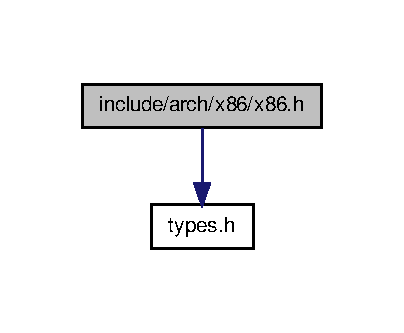
\includegraphics[width=194pt]{x86_8h__incl}
\end{center}
\end{figure}
\-This graph shows which files directly or indirectly include this file\-:\nopagebreak
\begin{figure}[H]
\begin{center}
\leavevmode
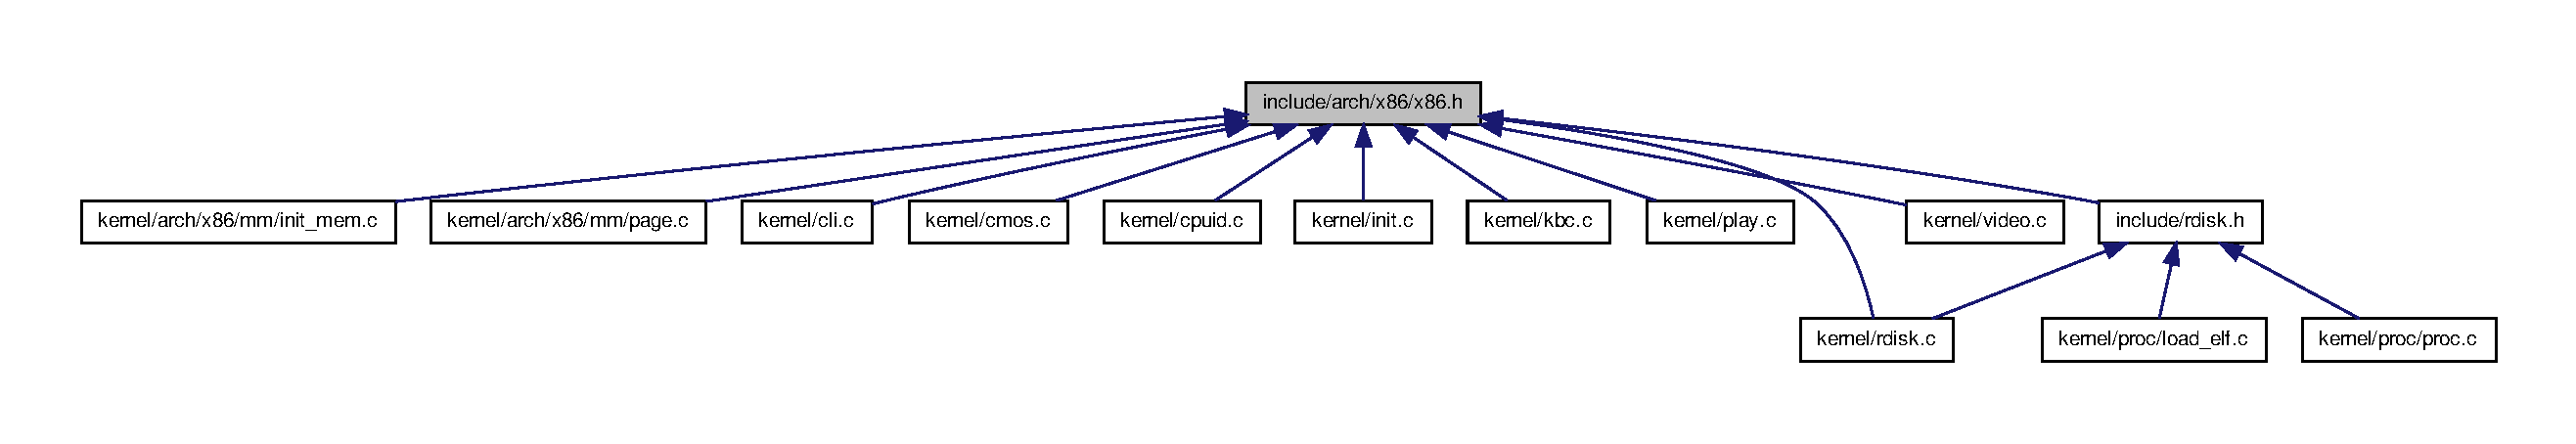
\includegraphics[width=350pt]{x86_8h__dep__incl}
\end{center}
\end{figure}
\subsection*{\-Functions}
\begin{DoxyCompactItemize}
\item 
static \-\_\-\-\_\-inline void \hyperlink{x86_8h_aecb1fa8a11c8a27335665526fc820dc6}{outb} (\hyperlink{types_8h_aba7bc1797add20fe3efdf37ced1182c5}{uint8\-\_\-t} data, int port)
\item 
static \-\_\-\-\_\-inline \hyperlink{types_8h_aba7bc1797add20fe3efdf37ced1182c5}{uint8\-\_\-t} \hyperlink{x86_8h_ab22bd329c089d76a3977792a2208f6b4}{inb} (int port)
\item 
static void \hyperlink{x86_8h_a6f3997e6e71bf8244d7619e557e96321}{outw} (\hyperlink{types_8h_a273cf69d639a59973b6019625df33e30}{uint16\-\_\-t} data, int port)
\item 
static \hyperlink{types_8h_a273cf69d639a59973b6019625df33e30}{uint16\-\_\-t} \hyperlink{x86_8h_a2140f94851a8b17db07aa505613d9e3e}{inw} (int port)
\item 
static \-\_\-\-\_\-inline void \hyperlink{x86_8h_af7e67ef5bbfeea2daede4f6b20d2eed1}{outl} (\hyperlink{types_8h_a435d1572bf3f880d55459d9805097f62}{uint32\-\_\-t} data, int port)
\item 
static \hyperlink{types_8h_a435d1572bf3f880d55459d9805097f62}{uint32\-\_\-t} \hyperlink{x86_8h_a4dc39efad1eea8befe2658287ec39913}{inl} (int port)
\item 
static void \hyperlink{x86_8h_a962d8e5318b592147d422996b0d86251}{insb} (void $\ast$addr, int cnt, int port)
\item 
static void \hyperlink{x86_8h_a16386395d1cae950f2efd9bed742d487}{insl} (void $\ast$addr, int cnt, int port)
\item 
static void \hyperlink{x86_8h_a366f523dd832c3fddeb78aefa3d96a82}{insw} (void $\ast$addr, int cnt, int port)
\item 
static void \hyperlink{x86_8h_a89d04efedb6dc6e8d87c6a5b453529e1}{cli} (void)
\item 
static void \hyperlink{x86_8h_af87d69b8449fc86a02b250af121cd29d}{sti} (void)
\item 
static void \hyperlink{x86_8h_abbf058df03c75df2ccb323b988f111cd}{write\-\_\-cr0} (\hyperlink{types_8h_a435d1572bf3f880d55459d9805097f62}{uint32\-\_\-t} value)
\item 
static \hyperlink{types_8h_a435d1572bf3f880d55459d9805097f62}{uint32\-\_\-t} \hyperlink{x86_8h_a5633092eb6843f453946c2471e89d698}{read\-\_\-cr0} (void)
\item 
static void \hyperlink{x86_8h_ad54b4fe02c9a2066abe07447f23909fc}{write\-\_\-cr1} (\hyperlink{types_8h_a435d1572bf3f880d55459d9805097f62}{uint32\-\_\-t} value)
\item 
static \hyperlink{types_8h_a435d1572bf3f880d55459d9805097f62}{uint32\-\_\-t} \hyperlink{x86_8h_aee9070b37bd064134b5f34667bbbd80a}{read\-\_\-cr1} (void)
\item 
static void \hyperlink{x86_8h_a2dfd7ac5612514e31c83fd0d1c33cd43}{write\-\_\-cr2} (\hyperlink{types_8h_a435d1572bf3f880d55459d9805097f62}{uint32\-\_\-t} value)
\item 
static \hyperlink{types_8h_a435d1572bf3f880d55459d9805097f62}{uint32\-\_\-t} \hyperlink{x86_8h_ae59d0287cd7ded2cf508fb87f00dfb69}{read\-\_\-cr2} (void)
\item 
static void \hyperlink{x86_8h_aad2f9353d3c5b5125eff2528008e0a6c}{write\-\_\-cr3} (\hyperlink{types_8h_a435d1572bf3f880d55459d9805097f62}{uint32\-\_\-t} value)
\item 
static \hyperlink{types_8h_a435d1572bf3f880d55459d9805097f62}{uint32\-\_\-t} \hyperlink{x86_8h_a2eefecfe0fd4c7aacb8787cf6b23728f}{read\-\_\-cr3} (void)
\item 
static void \hyperlink{x86_8h_a16adfa2cdde4a35215a6e2f2064c0bd8}{write\-\_\-cr4} (\hyperlink{types_8h_a435d1572bf3f880d55459d9805097f62}{uint32\-\_\-t} value)
\item 
static \hyperlink{types_8h_a435d1572bf3f880d55459d9805097f62}{uint32\-\_\-t} \hyperlink{x86_8h_a89c619dea6e47c6ffd62d651197b155e}{read\-\_\-cr4} (void)
\item 
static void \hyperlink{x86_8h_a3f418deaaaea7fb803f588fcb7c7c9b8}{cpuid} ()
\item 
static void \hyperlink{x86_8h_a2c1c4c8523ed258a75c563a8f94d1686}{invlpg} (void $\ast$addr)
\item 
static void \hyperlink{x86_8h_a0f221cad21039bde362eb1ef6114a639}{write\-\_\-tr} (\hyperlink{types_8h_a273cf69d639a59973b6019625df33e30}{uint16\-\_\-t} selector)
\item 
static \hyperlink{types_8h_a435d1572bf3f880d55459d9805097f62}{uint32\-\_\-t} \hyperlink{x86_8h_a3a5591d5247a312546086e48f215ad78}{read\-\_\-esp} (void)
\end{DoxyCompactItemize}


\subsection{\-Function \-Documentation}
\hypertarget{x86_8h_a89d04efedb6dc6e8d87c6a5b453529e1}{\index{x86.\-h@{x86.\-h}!cli@{cli}}
\index{cli@{cli}!x86.h@{x86.\-h}}
\subsubsection[{cli}]{\setlength{\rightskip}{0pt plus 5cm}static void {\bf cli} (
\begin{DoxyParamCaption}
\item[{void}]{}
\end{DoxyParamCaption}
)\hspace{0.3cm}{\ttfamily  \mbox{[}inline, static\mbox{]}}}}\label{x86_8h_a89d04efedb6dc6e8d87c6a5b453529e1}


\-Definition at line 60 of file x86.\-h.

\hypertarget{x86_8h_a3f418deaaaea7fb803f588fcb7c7c9b8}{\index{x86.\-h@{x86.\-h}!cpuid@{cpuid}}
\index{cpuid@{cpuid}!x86.h@{x86.\-h}}
\subsubsection[{cpuid}]{\setlength{\rightskip}{0pt plus 5cm}static void {\bf cpuid} (
\begin{DoxyParamCaption}
{}
\end{DoxyParamCaption}
)\hspace{0.3cm}{\ttfamily  \mbox{[}inline, static\mbox{]}}}}\label{x86_8h_a3f418deaaaea7fb803f588fcb7c7c9b8}


\-Definition at line 126 of file x86.\-h.

\hypertarget{x86_8h_ab22bd329c089d76a3977792a2208f6b4}{\index{x86.\-h@{x86.\-h}!inb@{inb}}
\index{inb@{inb}!x86.h@{x86.\-h}}
\subsubsection[{inb}]{\setlength{\rightskip}{0pt plus 5cm}static \-\_\-\-\_\-inline {\bf uint8\-\_\-t} {\bf inb} (
\begin{DoxyParamCaption}
\item[{int}]{port}
\end{DoxyParamCaption}
)\hspace{0.3cm}{\ttfamily  \mbox{[}static\mbox{]}}}}\label{x86_8h_ab22bd329c089d76a3977792a2208f6b4}


\-Definition at line 14 of file x86.\-h.

\hypertarget{x86_8h_a4dc39efad1eea8befe2658287ec39913}{\index{x86.\-h@{x86.\-h}!inl@{inl}}
\index{inl@{inl}!x86.h@{x86.\-h}}
\subsubsection[{inl}]{\setlength{\rightskip}{0pt plus 5cm}static {\bf uint32\-\_\-t} {\bf inl} (
\begin{DoxyParamCaption}
\item[{int}]{port}
\end{DoxyParamCaption}
)\hspace{0.3cm}{\ttfamily  \mbox{[}inline, static\mbox{]}}}}\label{x86_8h_a4dc39efad1eea8befe2658287ec39913}


\-Definition at line 36 of file x86.\-h.

\hypertarget{x86_8h_a962d8e5318b592147d422996b0d86251}{\index{x86.\-h@{x86.\-h}!insb@{insb}}
\index{insb@{insb}!x86.h@{x86.\-h}}
\subsubsection[{insb}]{\setlength{\rightskip}{0pt plus 5cm}static void {\bf insb} (
\begin{DoxyParamCaption}
\item[{void $\ast$}]{addr, }
\item[{int}]{cnt, }
\item[{int}]{port}
\end{DoxyParamCaption}
)\hspace{0.3cm}{\ttfamily  \mbox{[}inline, static\mbox{]}}}}\label{x86_8h_a962d8e5318b592147d422996b0d86251}


\-Definition at line 42 of file x86.\-h.

\hypertarget{x86_8h_a16386395d1cae950f2efd9bed742d487}{\index{x86.\-h@{x86.\-h}!insl@{insl}}
\index{insl@{insl}!x86.h@{x86.\-h}}
\subsubsection[{insl}]{\setlength{\rightskip}{0pt plus 5cm}static void {\bf insl} (
\begin{DoxyParamCaption}
\item[{void $\ast$}]{addr, }
\item[{int}]{cnt, }
\item[{int}]{port}
\end{DoxyParamCaption}
)\hspace{0.3cm}{\ttfamily  \mbox{[}inline, static\mbox{]}}}}\label{x86_8h_a16386395d1cae950f2efd9bed742d487}


\-Definition at line 48 of file x86.\-h.

\hypertarget{x86_8h_a366f523dd832c3fddeb78aefa3d96a82}{\index{x86.\-h@{x86.\-h}!insw@{insw}}
\index{insw@{insw}!x86.h@{x86.\-h}}
\subsubsection[{insw}]{\setlength{\rightskip}{0pt plus 5cm}static void {\bf insw} (
\begin{DoxyParamCaption}
\item[{void $\ast$}]{addr, }
\item[{int}]{cnt, }
\item[{int}]{port}
\end{DoxyParamCaption}
)\hspace{0.3cm}{\ttfamily  \mbox{[}inline, static\mbox{]}}}}\label{x86_8h_a366f523dd832c3fddeb78aefa3d96a82}


\-Definition at line 54 of file x86.\-h.

\hypertarget{x86_8h_a2c1c4c8523ed258a75c563a8f94d1686}{\index{x86.\-h@{x86.\-h}!invlpg@{invlpg}}
\index{invlpg@{invlpg}!x86.h@{x86.\-h}}
\subsubsection[{invlpg}]{\setlength{\rightskip}{0pt plus 5cm}static void {\bf invlpg} (
\begin{DoxyParamCaption}
\item[{void $\ast$}]{addr}
\end{DoxyParamCaption}
)\hspace{0.3cm}{\ttfamily  \mbox{[}inline, static\mbox{]}}}}\label{x86_8h_a2c1c4c8523ed258a75c563a8f94d1686}


\-Definition at line 131 of file x86.\-h.

\hypertarget{x86_8h_a2140f94851a8b17db07aa505613d9e3e}{\index{x86.\-h@{x86.\-h}!inw@{inw}}
\index{inw@{inw}!x86.h@{x86.\-h}}
\subsubsection[{inw}]{\setlength{\rightskip}{0pt plus 5cm}static {\bf uint16\-\_\-t} {\bf inw} (
\begin{DoxyParamCaption}
\item[{int}]{port}
\end{DoxyParamCaption}
)\hspace{0.3cm}{\ttfamily  \mbox{[}inline, static\mbox{]}}}}\label{x86_8h_a2140f94851a8b17db07aa505613d9e3e}


\-Definition at line 25 of file x86.\-h.

\hypertarget{x86_8h_aecb1fa8a11c8a27335665526fc820dc6}{\index{x86.\-h@{x86.\-h}!outb@{outb}}
\index{outb@{outb}!x86.h@{x86.\-h}}
\subsubsection[{outb}]{\setlength{\rightskip}{0pt plus 5cm}static \-\_\-\-\_\-inline void {\bf outb} (
\begin{DoxyParamCaption}
\item[{{\bf uint8\-\_\-t}}]{data, }
\item[{int}]{port}
\end{DoxyParamCaption}
)\hspace{0.3cm}{\ttfamily  \mbox{[}static\mbox{]}}}}\label{x86_8h_aecb1fa8a11c8a27335665526fc820dc6}


\-Definition at line 10 of file x86.\-h.

\hypertarget{x86_8h_af7e67ef5bbfeea2daede4f6b20d2eed1}{\index{x86.\-h@{x86.\-h}!outl@{outl}}
\index{outl@{outl}!x86.h@{x86.\-h}}
\subsubsection[{outl}]{\setlength{\rightskip}{0pt plus 5cm}static \-\_\-\-\_\-inline void {\bf outl} (
\begin{DoxyParamCaption}
\item[{{\bf uint32\-\_\-t}}]{data, }
\item[{int}]{port}
\end{DoxyParamCaption}
)\hspace{0.3cm}{\ttfamily  \mbox{[}static\mbox{]}}}}\label{x86_8h_af7e67ef5bbfeea2daede4f6b20d2eed1}


\-Definition at line 31 of file x86.\-h.

\hypertarget{x86_8h_a6f3997e6e71bf8244d7619e557e96321}{\index{x86.\-h@{x86.\-h}!outw@{outw}}
\index{outw@{outw}!x86.h@{x86.\-h}}
\subsubsection[{outw}]{\setlength{\rightskip}{0pt plus 5cm}static void {\bf outw} (
\begin{DoxyParamCaption}
\item[{{\bf uint16\-\_\-t}}]{data, }
\item[{int}]{port}
\end{DoxyParamCaption}
)\hspace{0.3cm}{\ttfamily  \mbox{[}inline, static\mbox{]}}}}\label{x86_8h_a6f3997e6e71bf8244d7619e557e96321}


\-Definition at line 20 of file x86.\-h.

\hypertarget{x86_8h_a5633092eb6843f453946c2471e89d698}{\index{x86.\-h@{x86.\-h}!read\-\_\-cr0@{read\-\_\-cr0}}
\index{read\-\_\-cr0@{read\-\_\-cr0}!x86.h@{x86.\-h}}
\subsubsection[{read\-\_\-cr0}]{\setlength{\rightskip}{0pt plus 5cm}static {\bf uint32\-\_\-t} {\bf read\-\_\-cr0} (
\begin{DoxyParamCaption}
\item[{void}]{}
\end{DoxyParamCaption}
)\hspace{0.3cm}{\ttfamily  \mbox{[}inline, static\mbox{]}}}}\label{x86_8h_a5633092eb6843f453946c2471e89d698}


\-Definition at line 72 of file x86.\-h.

\hypertarget{x86_8h_aee9070b37bd064134b5f34667bbbd80a}{\index{x86.\-h@{x86.\-h}!read\-\_\-cr1@{read\-\_\-cr1}}
\index{read\-\_\-cr1@{read\-\_\-cr1}!x86.h@{x86.\-h}}
\subsubsection[{read\-\_\-cr1}]{\setlength{\rightskip}{0pt plus 5cm}static {\bf uint32\-\_\-t} {\bf read\-\_\-cr1} (
\begin{DoxyParamCaption}
\item[{void}]{}
\end{DoxyParamCaption}
)\hspace{0.3cm}{\ttfamily  \mbox{[}inline, static\mbox{]}}}}\label{x86_8h_aee9070b37bd064134b5f34667bbbd80a}


\-Definition at line 84 of file x86.\-h.

\hypertarget{x86_8h_ae59d0287cd7ded2cf508fb87f00dfb69}{\index{x86.\-h@{x86.\-h}!read\-\_\-cr2@{read\-\_\-cr2}}
\index{read\-\_\-cr2@{read\-\_\-cr2}!x86.h@{x86.\-h}}
\subsubsection[{read\-\_\-cr2}]{\setlength{\rightskip}{0pt plus 5cm}static {\bf uint32\-\_\-t} {\bf read\-\_\-cr2} (
\begin{DoxyParamCaption}
\item[{void}]{}
\end{DoxyParamCaption}
)\hspace{0.3cm}{\ttfamily  \mbox{[}inline, static\mbox{]}}}}\label{x86_8h_ae59d0287cd7ded2cf508fb87f00dfb69}


\-Definition at line 96 of file x86.\-h.

\hypertarget{x86_8h_a2eefecfe0fd4c7aacb8787cf6b23728f}{\index{x86.\-h@{x86.\-h}!read\-\_\-cr3@{read\-\_\-cr3}}
\index{read\-\_\-cr3@{read\-\_\-cr3}!x86.h@{x86.\-h}}
\subsubsection[{read\-\_\-cr3}]{\setlength{\rightskip}{0pt plus 5cm}static {\bf uint32\-\_\-t} {\bf read\-\_\-cr3} (
\begin{DoxyParamCaption}
\item[{void}]{}
\end{DoxyParamCaption}
)\hspace{0.3cm}{\ttfamily  \mbox{[}inline, static\mbox{]}}}}\label{x86_8h_a2eefecfe0fd4c7aacb8787cf6b23728f}


\-Definition at line 108 of file x86.\-h.

\hypertarget{x86_8h_a89c619dea6e47c6ffd62d651197b155e}{\index{x86.\-h@{x86.\-h}!read\-\_\-cr4@{read\-\_\-cr4}}
\index{read\-\_\-cr4@{read\-\_\-cr4}!x86.h@{x86.\-h}}
\subsubsection[{read\-\_\-cr4}]{\setlength{\rightskip}{0pt plus 5cm}static {\bf uint32\-\_\-t} {\bf read\-\_\-cr4} (
\begin{DoxyParamCaption}
\item[{void}]{}
\end{DoxyParamCaption}
)\hspace{0.3cm}{\ttfamily  \mbox{[}inline, static\mbox{]}}}}\label{x86_8h_a89c619dea6e47c6ffd62d651197b155e}


\-Definition at line 120 of file x86.\-h.

\hypertarget{x86_8h_a3a5591d5247a312546086e48f215ad78}{\index{x86.\-h@{x86.\-h}!read\-\_\-esp@{read\-\_\-esp}}
\index{read\-\_\-esp@{read\-\_\-esp}!x86.h@{x86.\-h}}
\subsubsection[{read\-\_\-esp}]{\setlength{\rightskip}{0pt plus 5cm}static {\bf uint32\-\_\-t} {\bf read\-\_\-esp} (
\begin{DoxyParamCaption}
\item[{void}]{}
\end{DoxyParamCaption}
)\hspace{0.3cm}{\ttfamily  \mbox{[}inline, static\mbox{]}}}}\label{x86_8h_a3a5591d5247a312546086e48f215ad78}


\-Definition at line 142 of file x86.\-h.

\hypertarget{x86_8h_af87d69b8449fc86a02b250af121cd29d}{\index{x86.\-h@{x86.\-h}!sti@{sti}}
\index{sti@{sti}!x86.h@{x86.\-h}}
\subsubsection[{sti}]{\setlength{\rightskip}{0pt plus 5cm}static void {\bf sti} (
\begin{DoxyParamCaption}
\item[{void}]{}
\end{DoxyParamCaption}
)\hspace{0.3cm}{\ttfamily  \mbox{[}inline, static\mbox{]}}}}\label{x86_8h_af87d69b8449fc86a02b250af121cd29d}


\-Definition at line 63 of file x86.\-h.

\hypertarget{x86_8h_abbf058df03c75df2ccb323b988f111cd}{\index{x86.\-h@{x86.\-h}!write\-\_\-cr0@{write\-\_\-cr0}}
\index{write\-\_\-cr0@{write\-\_\-cr0}!x86.h@{x86.\-h}}
\subsubsection[{write\-\_\-cr0}]{\setlength{\rightskip}{0pt plus 5cm}static void {\bf write\-\_\-cr0} (
\begin{DoxyParamCaption}
\item[{{\bf uint32\-\_\-t}}]{value}
\end{DoxyParamCaption}
)\hspace{0.3cm}{\ttfamily  \mbox{[}inline, static\mbox{]}}}}\label{x86_8h_abbf058df03c75df2ccb323b988f111cd}


\-Definition at line 67 of file x86.\-h.

\hypertarget{x86_8h_ad54b4fe02c9a2066abe07447f23909fc}{\index{x86.\-h@{x86.\-h}!write\-\_\-cr1@{write\-\_\-cr1}}
\index{write\-\_\-cr1@{write\-\_\-cr1}!x86.h@{x86.\-h}}
\subsubsection[{write\-\_\-cr1}]{\setlength{\rightskip}{0pt plus 5cm}static void {\bf write\-\_\-cr1} (
\begin{DoxyParamCaption}
\item[{{\bf uint32\-\_\-t}}]{value}
\end{DoxyParamCaption}
)\hspace{0.3cm}{\ttfamily  \mbox{[}inline, static\mbox{]}}}}\label{x86_8h_ad54b4fe02c9a2066abe07447f23909fc}


\-Definition at line 79 of file x86.\-h.

\hypertarget{x86_8h_a2dfd7ac5612514e31c83fd0d1c33cd43}{\index{x86.\-h@{x86.\-h}!write\-\_\-cr2@{write\-\_\-cr2}}
\index{write\-\_\-cr2@{write\-\_\-cr2}!x86.h@{x86.\-h}}
\subsubsection[{write\-\_\-cr2}]{\setlength{\rightskip}{0pt plus 5cm}static void {\bf write\-\_\-cr2} (
\begin{DoxyParamCaption}
\item[{{\bf uint32\-\_\-t}}]{value}
\end{DoxyParamCaption}
)\hspace{0.3cm}{\ttfamily  \mbox{[}inline, static\mbox{]}}}}\label{x86_8h_a2dfd7ac5612514e31c83fd0d1c33cd43}


\-Definition at line 91 of file x86.\-h.

\hypertarget{x86_8h_aad2f9353d3c5b5125eff2528008e0a6c}{\index{x86.\-h@{x86.\-h}!write\-\_\-cr3@{write\-\_\-cr3}}
\index{write\-\_\-cr3@{write\-\_\-cr3}!x86.h@{x86.\-h}}
\subsubsection[{write\-\_\-cr3}]{\setlength{\rightskip}{0pt plus 5cm}static void {\bf write\-\_\-cr3} (
\begin{DoxyParamCaption}
\item[{{\bf uint32\-\_\-t}}]{value}
\end{DoxyParamCaption}
)\hspace{0.3cm}{\ttfamily  \mbox{[}inline, static\mbox{]}}}}\label{x86_8h_aad2f9353d3c5b5125eff2528008e0a6c}


\-Definition at line 103 of file x86.\-h.

\hypertarget{x86_8h_a16adfa2cdde4a35215a6e2f2064c0bd8}{\index{x86.\-h@{x86.\-h}!write\-\_\-cr4@{write\-\_\-cr4}}
\index{write\-\_\-cr4@{write\-\_\-cr4}!x86.h@{x86.\-h}}
\subsubsection[{write\-\_\-cr4}]{\setlength{\rightskip}{0pt plus 5cm}static void {\bf write\-\_\-cr4} (
\begin{DoxyParamCaption}
\item[{{\bf uint32\-\_\-t}}]{value}
\end{DoxyParamCaption}
)\hspace{0.3cm}{\ttfamily  \mbox{[}inline, static\mbox{]}}}}\label{x86_8h_a16adfa2cdde4a35215a6e2f2064c0bd8}


\-Definition at line 115 of file x86.\-h.

\hypertarget{x86_8h_a0f221cad21039bde362eb1ef6114a639}{\index{x86.\-h@{x86.\-h}!write\-\_\-tr@{write\-\_\-tr}}
\index{write\-\_\-tr@{write\-\_\-tr}!x86.h@{x86.\-h}}
\subsubsection[{write\-\_\-tr}]{\setlength{\rightskip}{0pt plus 5cm}static void {\bf write\-\_\-tr} (
\begin{DoxyParamCaption}
\item[{{\bf uint16\-\_\-t}}]{selector}
\end{DoxyParamCaption}
)\hspace{0.3cm}{\ttfamily  \mbox{[}inline, static\mbox{]}}}}\label{x86_8h_a0f221cad21039bde362eb1ef6114a639}


\-Definition at line 137 of file x86.\-h.


\hypertarget{cli_8h}{\section{include/cli.h \-File \-Reference}
\label{cli_8h}\index{include/cli.\-h@{include/cli.\-h}}
}
\-This graph shows which files directly or indirectly include this file\-:\nopagebreak
\begin{figure}[H]
\begin{center}
\leavevmode
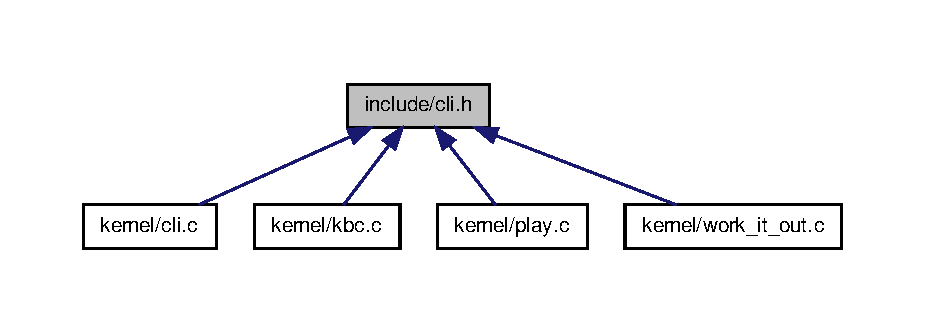
\includegraphics[width=350pt]{cli_8h__dep__incl}
\end{center}
\end{figure}
\subsection*{\-Defines}
\begin{DoxyCompactItemize}
\item 
\#define \hyperlink{cli_8h_a848bb0e0fe1522d44344445c43d05bec}{\-M\-A\-X\-B\-U\-F\-S\-I\-Z\-E}~512
\end{DoxyCompactItemize}
\subsection*{\-Functions}
\begin{DoxyCompactItemize}
\item 
void \hyperlink{cli_8h_acadd2a5d99d952e55a4580dbc8f8739d}{console\-\_\-init} (void)
\item 
void \hyperlink{cli_8h_a3c8b2e35ff573401b1df8d0938cf75e6}{console\-\_\-interrupt} (int($\ast$intr)(void))
\item 
int \hyperlink{cli_8h_a9b3ba9ca613021d6954ade2927d8d56e}{console\-\_\-getc} (void)
\item 
void \hyperlink{cli_8h_ad3429ca65a1b6f39eed6d2f9f795586b}{console\-\_\-putc} (int c)
\end{DoxyCompactItemize}
\subsection*{\-Variables}
\begin{DoxyCompactItemize}
\item 
\begin{tabbing}
xx\=xx\=xx\=xx\=xx\=xx\=xx\=xx\=xx\=\kill
struct \{\\
\>\hyperlink{types_8h_aba7bc1797add20fe3efdf37ced1182c5}{uint8\_t} \hyperlink{cli_8h_aa6145441e2e882d75ecf178941990f7a}{buf} \mbox{[}\hyperlink{cli_8h_a848bb0e0fe1522d44344445c43d05bec}{MAXBUFSIZE}\mbox{]}\\
\>\hyperlink{types_8h_a435d1572bf3f880d55459d9805097f62}{uint32\_t} \hyperlink{cli_8h_a1c505fee165286dfd12c0029ba4ff10b}{rpos}\\
\>\hyperlink{types_8h_a435d1572bf3f880d55459d9805097f62}{uint32\_t} \hyperlink{cli_8h_aa2f2555221255b51b0d19da27e6e8877}{wpos}\\
\} \hyperlink{cli_8h_aab9656ee89b6ea3f72abaff0275333d4}{cons}\\

\end{tabbing}\end{DoxyCompactItemize}


\subsection{\-Define \-Documentation}
\hypertarget{cli_8h_a848bb0e0fe1522d44344445c43d05bec}{\index{cli.\-h@{cli.\-h}!\-M\-A\-X\-B\-U\-F\-S\-I\-Z\-E@{\-M\-A\-X\-B\-U\-F\-S\-I\-Z\-E}}
\index{\-M\-A\-X\-B\-U\-F\-S\-I\-Z\-E@{\-M\-A\-X\-B\-U\-F\-S\-I\-Z\-E}!cli.h@{cli.\-h}}
\subsubsection[{\-M\-A\-X\-B\-U\-F\-S\-I\-Z\-E}]{\setlength{\rightskip}{0pt plus 5cm}\#define {\bf \-M\-A\-X\-B\-U\-F\-S\-I\-Z\-E}~512}}\label{cli_8h_a848bb0e0fe1522d44344445c43d05bec}


\-Definition at line 8 of file cli.\-h.



\subsection{\-Function \-Documentation}
\hypertarget{cli_8h_a9b3ba9ca613021d6954ade2927d8d56e}{\index{cli.\-h@{cli.\-h}!console\-\_\-getc@{console\-\_\-getc}}
\index{console\-\_\-getc@{console\-\_\-getc}!cli.h@{cli.\-h}}
\subsubsection[{console\-\_\-getc}]{\setlength{\rightskip}{0pt plus 5cm}int {\bf console\-\_\-getc} (
\begin{DoxyParamCaption}
\item[{void}]{}
\end{DoxyParamCaption}
)}}\label{cli_8h_a9b3ba9ca613021d6954ade2927d8d56e}


\-Definition at line 32 of file cli.\-c.

\hypertarget{cli_8h_acadd2a5d99d952e55a4580dbc8f8739d}{\index{cli.\-h@{cli.\-h}!console\-\_\-init@{console\-\_\-init}}
\index{console\-\_\-init@{console\-\_\-init}!cli.h@{cli.\-h}}
\subsubsection[{console\-\_\-init}]{\setlength{\rightskip}{0pt plus 5cm}void {\bf console\-\_\-init} (
\begin{DoxyParamCaption}
\item[{void}]{}
\end{DoxyParamCaption}
)}}\label{cli_8h_acadd2a5d99d952e55a4580dbc8f8739d}


\-Definition at line 8 of file cli.\-c.

\hypertarget{cli_8h_a3c8b2e35ff573401b1df8d0938cf75e6}{\index{cli.\-h@{cli.\-h}!console\-\_\-interrupt@{console\-\_\-interrupt}}
\index{console\-\_\-interrupt@{console\-\_\-interrupt}!cli.h@{cli.\-h}}
\subsubsection[{console\-\_\-interrupt}]{\setlength{\rightskip}{0pt plus 5cm}void {\bf console\-\_\-interrupt} (
\begin{DoxyParamCaption}
\item[{int($\ast$)(void)}]{intr}
\end{DoxyParamCaption}
)}}\label{cli_8h_a3c8b2e35ff573401b1df8d0938cf75e6}


\-Definition at line 16 of file cli.\-c.

\hypertarget{cli_8h_ad3429ca65a1b6f39eed6d2f9f795586b}{\index{cli.\-h@{cli.\-h}!console\-\_\-putc@{console\-\_\-putc}}
\index{console\-\_\-putc@{console\-\_\-putc}!cli.h@{cli.\-h}}
\subsubsection[{console\-\_\-putc}]{\setlength{\rightskip}{0pt plus 5cm}void {\bf console\-\_\-putc} (
\begin{DoxyParamCaption}
\item[{int}]{c}
\end{DoxyParamCaption}
)}}\label{cli_8h_ad3429ca65a1b6f39eed6d2f9f795586b}


\-Definition at line 45 of file cli.\-c.



\subsection{\-Variable \-Documentation}
\hypertarget{cli_8h_aa6145441e2e882d75ecf178941990f7a}{\index{cli.\-h@{cli.\-h}!buf@{buf}}
\index{buf@{buf}!cli.h@{cli.\-h}}
\subsubsection[{buf}]{\setlength{\rightskip}{0pt plus 5cm}{\bf uint8\-\_\-t} {\bf buf}\mbox{[}{\bf \-M\-A\-X\-B\-U\-F\-S\-I\-Z\-E}\mbox{]}}}\label{cli_8h_aa6145441e2e882d75ecf178941990f7a}


\-Definition at line 14 of file cli.\-h.

\hypertarget{cli_8h_aab9656ee89b6ea3f72abaff0275333d4}{\index{cli.\-h@{cli.\-h}!cons@{cons}}
\index{cons@{cons}!cli.h@{cli.\-h}}
\subsubsection[{cons}]{\setlength{\rightskip}{0pt plus 5cm}struct \{ ... \}   {\bf cons}\hspace{0.3cm}{\ttfamily  \mbox{[}static\mbox{]}}}}\label{cli_8h_aab9656ee89b6ea3f72abaff0275333d4}
\hypertarget{cli_8h_a1c505fee165286dfd12c0029ba4ff10b}{\index{cli.\-h@{cli.\-h}!rpos@{rpos}}
\index{rpos@{rpos}!cli.h@{cli.\-h}}
\subsubsection[{rpos}]{\setlength{\rightskip}{0pt plus 5cm}{\bf uint32\-\_\-t} {\bf rpos}}}\label{cli_8h_a1c505fee165286dfd12c0029ba4ff10b}


\-Definition at line 15 of file cli.\-h.

\hypertarget{cli_8h_aa2f2555221255b51b0d19da27e6e8877}{\index{cli.\-h@{cli.\-h}!wpos@{wpos}}
\index{wpos@{wpos}!cli.h@{cli.\-h}}
\subsubsection[{wpos}]{\setlength{\rightskip}{0pt plus 5cm}{\bf uint32\-\_\-t} {\bf wpos}}}\label{cli_8h_aa2f2555221255b51b0d19da27e6e8877}


\-Definition at line 16 of file cli.\-h.


\hypertarget{cmos_8h}{\section{include/cmos.h \-File \-Reference}
\label{cmos_8h}\index{include/cmos.\-h@{include/cmos.\-h}}
}
\-This graph shows which files directly or indirectly include this file\-:\nopagebreak
\begin{figure}[H]
\begin{center}
\leavevmode
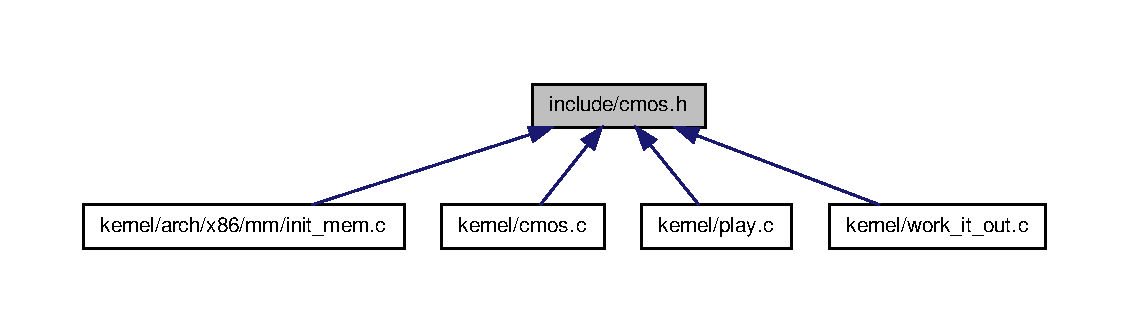
\includegraphics[width=350pt]{cmos_8h__dep__incl}
\end{center}
\end{figure}
\subsection*{\-Defines}
\begin{DoxyCompactItemize}
\item 
\#define \hyperlink{cmos_8h_aab1aadc621607164a95a5e215c87f8a1}{\-C\-M\-O\-S\-\_\-\-I\-N\-D\-E\-X\-P\-O\-R\-T}~0x70	/$\ast$ the C\-M\-O\-S/\-R\-T\-C index register port $\ast$/
\item 
\#define \hyperlink{cmos_8h_ad771171173789dbfd8c86a9ad348d66e}{\-C\-M\-O\-S\-\_\-\-D\-A\-T\-A\-P\-O\-R\-T}~0x71	/$\ast$ the C\-M\-O\-S/\-R\-T\-C data register port $\ast$/
\item 
\#define \hyperlink{cmos_8h_a43f6540c6d3a78b930f9adad56cf7fac}{\-R\-T\-C\-\_\-\-S\-E\-C\-O\-N\-D\-S}~0x0
\item 
\#define \hyperlink{cmos_8h_a8ffbdf491195260a4eedf5f87951b812}{\-R\-T\-C\-\_\-\-A\-L\-R\-M\-S\-E\-C\-O\-N\-D}~0x1
\item 
\#define \hyperlink{cmos_8h_aabc0725ac27ea93c913a2a4d7cd51ac7}{\-R\-T\-C\-\_\-\-M\-I\-N\-U\-T\-E\-S}~0x2
\item 
\#define \hyperlink{cmos_8h_a465f91c1ca32a4de224d4070d48815f6}{\-R\-T\-C\-\_\-\-A\-L\-R\-M\-M\-I\-N\-U\-T\-E}~0x3
\item 
\#define \hyperlink{cmos_8h_a7264eac87ffc91cbdea1239d346a0ea4}{\-R\-T\-C\-\_\-\-H\-O\-U\-R}~0x4
\item 
\#define \hyperlink{cmos_8h_ad2ac2bf9afa2a4eb540c64d5c5018d49}{\-R\-T\-C\-\_\-\-A\-L\-R\-M\-H\-O\-U\-R}~0x5
\item 
\#define \hyperlink{cmos_8h_a5b232f7d613eb3e959f571cc1fa9609e}{\-R\-T\-C\-\_\-\-D\-A\-Y\-\_\-\-W\-E\-E\-K}~0x6
\item 
\#define \hyperlink{cmos_8h_a46fee80fd77bfe75bc9b6945e8676de8}{\-R\-T\-C\-\_\-\-D\-A\-Y\-\_\-\-M\-O\-N\-T\-H}~0x7
\item 
\#define \hyperlink{cmos_8h_abda0c877ee1a02b8351c0cfe72838088}{\-R\-T\-C\-\_\-\-M\-O\-N\-T\-H}~0x8
\item 
\#define \hyperlink{cmos_8h_a1df5568e6774b73aa4c6e59fc40e9147}{\-R\-T\-C\-\_\-\-Y\-E\-A\-R}~0x9
\item 
\#define \hyperlink{cmos_8h_ac5c524d4ff3b0ea39e957539e47f01d7}{\-R\-T\-C\-\_\-\-S\-T\-A\-T\-U\-S\-\_\-\-A}~0x\-A	/$\ast$ the R\-T\-C Status register A $\ast$/
\item 
\#define \hyperlink{cmos_8h_a7ed6b9349b7b7b18f4ea3244c523ab50}{\-R\-T\-C\-\_\-\-S\-T\-A\-T\-U\-S\-\_\-\-B}~0x\-B	/$\ast$ the R\-T\-C Status register B $\ast$/
\item 
\#define \hyperlink{cmos_8h_abd9109d33f6880a5eac5e82425f7398d}{\-S\-T\-A\-T\-\_\-\-R\-U\-N}~0x7\-F
\item 
\#define \hyperlink{cmos_8h_a0f25b982482e7b1db7867bbff240ee92}{\-S\-T\-A\-T\-\_\-\-H\-A\-L\-T}~0x80
\item 
\#define \hyperlink{cmos_8h_a9a446bfa7da9e2b7719316244306e661}{\-S\-T\-A\-T\-\_\-\-P\-E\-R\-\_\-\-I\-N\-T\-R}~0x40
\item 
\#define \hyperlink{cmos_8h_aae0bd1a44577807cbcc000e5f1199e04}{\-S\-T\-A\-T\-\_\-\-A\-L\-R\-M\-\_\-\-I\-N\-T\-R}~0x20
\item 
\#define \hyperlink{cmos_8h_a84b76f44cbf3554e0285b5cf226ea672}{\-S\-T\-A\-T\-\_\-\-U\-P\-D\-T\-\_\-\-I\-N\-T\-R}~0x10
\item 
\#define \hyperlink{cmos_8h_a37430a26f0b07bafe329dc1a89721185}{\-S\-T\-A\-T\-\_\-\-S\-Q\-R\-W\-V\-\_\-\-I\-N\-T\-R}~0x08
\item 
\#define \hyperlink{cmos_8h_aaf1fc69eb8a831f329ccba479f22a80b}{\-S\-T\-A\-T\-\_\-\-C\-A\-L\-\_\-\-B\-I\-N}~0x04
\item 
\#define \hyperlink{cmos_8h_a203e8a9fa78cd5cefdba7fbb53760254}{\-S\-T\-A\-T\-\_\-\-C\-A\-L\-\_\-\-B\-C\-D}~0x\-F\-B
\item 
\#define \hyperlink{cmos_8h_a323df7635c29ceab60f155caab754b2f}{\-S\-T\-A\-T\-\_\-\-C\-A\-L\-\_\-\-H\-R24}~0x02
\item 
\#define \hyperlink{cmos_8h_ac20af196d50bade782ffdcace7426d28}{\-S\-T\-A\-T\-\_\-\-C\-A\-L\-\_\-\-H\-R12}~0x\-F\-D
\item 
\#define \hyperlink{cmos_8h_a278243dd1c69407b80046b3d4a175d91}{\-S\-T\-A\-T\-\_\-\-D\-A\-Y\-\_\-\-L\-G\-H\-T}~0x01
\item 
\#define \hyperlink{cmos_8h_a5e0822d6e9720979c59b13ce2e11fa87}{\-C\-M\-O\-S\-\_\-\-S\-T\-A\-T\-U\-S\-\_\-\-C}~0x\-C
\item 
\#define \hyperlink{cmos_8h_ad63f234e0feaff2901f9895dd58bd6cd}{\-C\-M\-O\-S\-\_\-\-S\-T\-A\-T\-U\-S\-\_\-\-D}~0x\-D
\item 
\#define \hyperlink{cmos_8h_a3caabb2ecce2f1b95173e423dac736ae}{\-C\-M\-O\-S\-\_\-\-S\-T\-A\-T\-U\-S\-\_\-\-E}~0x\-E	/$\ast$ R\-T\-C diagnostic register E $\ast$/
\item 
\#define \hyperlink{cmos_8h_a9beb898210762fc0cf5f4cd965604700}{\-C\-M\-O\-S\-\_\-\-S\-T\-A\-T\-U\-S\-\_\-\-F}~0x\-F	/$\ast$ R\-T\-C Shut-\/down status register F $\ast$/
\item 
\#define \hyperlink{cmos_8h_a0eb09c1098c28e96955f0af8ad38a48a}{\-C\-M\-O\-S\-\_\-\-S\-T\-A\-T\-U\-S\-\_\-10}~0x10	/$\ast$ R\-T\-C D\-R\-I\-V\-E\-R T\-Y\-P\-E for A\-: and B\-: register $\ast$/
\item 
\#define \hyperlink{cmos_8h_a06eac64db0081da4cb67062adce92e39}{\-C\-M\-O\-S\-\_\-\-F\-I\-X\-E\-D\-\_\-\-D\-I\-S\-K}~0x12	/$\ast$ R\-T\-C Fixed disk drive type for drive 0 and drive 1 register $\ast$/
\item 
\#define \hyperlink{cmos_8h_ac6a198f84cf1868e5fe87068cab975c6}{\-C\-M\-O\-S\-\_\-\-E\-Q\-U\-I\-P\-\_\-\-B\-Y\-T\-E}~0x14	/$\ast$ R\-T\-C Equip byte $\ast$/
\item 
\#define \hyperlink{cmos_8h_a432dd72404fb14a3e5ba9a69e9bf547c}{\-C\-M\-O\-S\-\_\-\-S\-Y\-S\-B\-A\-S\-E\-\_\-\-L\-S\-B}~0x15	/$\ast$ L\-S\-B of System base memory in Kilo byte$\ast$/
\item 
\#define \hyperlink{cmos_8h_a2d8f232cffd1176677240cdab61cd4e4}{\-C\-M\-O\-S\-\_\-\-S\-Y\-S\-B\-A\-S\-E\-\_\-\-M\-S\-B}~0x16	/$\ast$ M\-S\-B of $\sim$$\sim$$\sim$$\sim$$\sim$$\sim$$\sim$$\sim$$\sim$$\sim$$\sim$$\sim$$\sim$$\sim$$\sim$$\sim$$\sim$$\sim$$\sim$$\sim$$\sim$$\sim$$\sim$$\sim$$\sim$$\sim$$\sim$$\sim$$\sim$$\sim$$\sim$$\ast$/
\item 
\#define \hyperlink{cmos_8h_a4dbf34401a2ed679242757fe4824919a}{\-C\-M\-O\-S\-\_\-\-E\-X\-T\-M\-E\-M\-\_\-\-L\-S\-B}~0x17	/$\ast$ L\-S\-B of total extended memory in Kilo byte $\ast$/
\item 
\#define \hyperlink{cmos_8h_a533854b7b52d19b1c8af0893a2816223}{\-C\-M\-O\-S\-\_\-\-E\-X\-T\-M\-E\-M\-\_\-\-M\-S\-B}~0x18	/$\ast$ M\-S\-B of $\sim$$\sim$$\sim$$\sim$$\sim$$\sim$$\sim$$\sim$$\sim$$\sim$$\sim$$\sim$$\sim$$\sim$$\sim$$\sim$$\sim$$\sim$$\sim$$\sim$$\sim$$\sim$$\sim$$\sim$$\sim$$\sim$$\sim$$\sim$$\sim$$\sim$$\sim$$\sim$$\sim$$\sim$ $\ast$/
\item 
\#define \hyperlink{cmos_8h_a362a7d20cb23f4b78bd8ca741d0cee0e}{\-C\-M\-O\-S\-\_\-\-D\-R\-I\-V\-E\-\_\-\-C}~0x19	/$\ast$ Drive C extention type $\ast$/
\item 
\#define \hyperlink{cmos_8h_a1fd110dd4665bd2d7d8e7b10f27b2758}{\-C\-M\-O\-S\-\_\-\-D\-R\-I\-V\-E\-\_\-\-D}~0x1\-A	/$\ast$ Drive D extention type $\ast$/
\end{DoxyCompactItemize}


\subsection{\-Define \-Documentation}
\hypertarget{cmos_8h_ad771171173789dbfd8c86a9ad348d66e}{\index{cmos.\-h@{cmos.\-h}!\-C\-M\-O\-S\-\_\-\-D\-A\-T\-A\-P\-O\-R\-T@{\-C\-M\-O\-S\-\_\-\-D\-A\-T\-A\-P\-O\-R\-T}}
\index{\-C\-M\-O\-S\-\_\-\-D\-A\-T\-A\-P\-O\-R\-T@{\-C\-M\-O\-S\-\_\-\-D\-A\-T\-A\-P\-O\-R\-T}!cmos.h@{cmos.\-h}}
\subsubsection[{\-C\-M\-O\-S\-\_\-\-D\-A\-T\-A\-P\-O\-R\-T}]{\setlength{\rightskip}{0pt plus 5cm}\#define {\bf \-C\-M\-O\-S\-\_\-\-D\-A\-T\-A\-P\-O\-R\-T}~0x71	/$\ast$ the C\-M\-O\-S/\-R\-T\-C data register port $\ast$/}}\label{cmos_8h_ad771171173789dbfd8c86a9ad348d66e}


\-Definition at line 10 of file cmos.\-h.

\hypertarget{cmos_8h_a362a7d20cb23f4b78bd8ca741d0cee0e}{\index{cmos.\-h@{cmos.\-h}!\-C\-M\-O\-S\-\_\-\-D\-R\-I\-V\-E\-\_\-\-C@{\-C\-M\-O\-S\-\_\-\-D\-R\-I\-V\-E\-\_\-\-C}}
\index{\-C\-M\-O\-S\-\_\-\-D\-R\-I\-V\-E\-\_\-\-C@{\-C\-M\-O\-S\-\_\-\-D\-R\-I\-V\-E\-\_\-\-C}!cmos.h@{cmos.\-h}}
\subsubsection[{\-C\-M\-O\-S\-\_\-\-D\-R\-I\-V\-E\-\_\-\-C}]{\setlength{\rightskip}{0pt plus 5cm}\#define {\bf \-C\-M\-O\-S\-\_\-\-D\-R\-I\-V\-E\-\_\-\-C}~0x19	/$\ast$ Drive C extention type $\ast$/}}\label{cmos_8h_a362a7d20cb23f4b78bd8ca741d0cee0e}


\-Definition at line 51 of file cmos.\-h.

\hypertarget{cmos_8h_a1fd110dd4665bd2d7d8e7b10f27b2758}{\index{cmos.\-h@{cmos.\-h}!\-C\-M\-O\-S\-\_\-\-D\-R\-I\-V\-E\-\_\-\-D@{\-C\-M\-O\-S\-\_\-\-D\-R\-I\-V\-E\-\_\-\-D}}
\index{\-C\-M\-O\-S\-\_\-\-D\-R\-I\-V\-E\-\_\-\-D@{\-C\-M\-O\-S\-\_\-\-D\-R\-I\-V\-E\-\_\-\-D}!cmos.h@{cmos.\-h}}
\subsubsection[{\-C\-M\-O\-S\-\_\-\-D\-R\-I\-V\-E\-\_\-\-D}]{\setlength{\rightskip}{0pt plus 5cm}\#define {\bf \-C\-M\-O\-S\-\_\-\-D\-R\-I\-V\-E\-\_\-\-D}~0x1\-A	/$\ast$ Drive D extention type $\ast$/}}\label{cmos_8h_a1fd110dd4665bd2d7d8e7b10f27b2758}


\-Definition at line 52 of file cmos.\-h.

\hypertarget{cmos_8h_ac6a198f84cf1868e5fe87068cab975c6}{\index{cmos.\-h@{cmos.\-h}!\-C\-M\-O\-S\-\_\-\-E\-Q\-U\-I\-P\-\_\-\-B\-Y\-T\-E@{\-C\-M\-O\-S\-\_\-\-E\-Q\-U\-I\-P\-\_\-\-B\-Y\-T\-E}}
\index{\-C\-M\-O\-S\-\_\-\-E\-Q\-U\-I\-P\-\_\-\-B\-Y\-T\-E@{\-C\-M\-O\-S\-\_\-\-E\-Q\-U\-I\-P\-\_\-\-B\-Y\-T\-E}!cmos.h@{cmos.\-h}}
\subsubsection[{\-C\-M\-O\-S\-\_\-\-E\-Q\-U\-I\-P\-\_\-\-B\-Y\-T\-E}]{\setlength{\rightskip}{0pt plus 5cm}\#define {\bf \-C\-M\-O\-S\-\_\-\-E\-Q\-U\-I\-P\-\_\-\-B\-Y\-T\-E}~0x14	/$\ast$ R\-T\-C Equip byte $\ast$/}}\label{cmos_8h_ac6a198f84cf1868e5fe87068cab975c6}


\-Definition at line 46 of file cmos.\-h.

\hypertarget{cmos_8h_a4dbf34401a2ed679242757fe4824919a}{\index{cmos.\-h@{cmos.\-h}!\-C\-M\-O\-S\-\_\-\-E\-X\-T\-M\-E\-M\-\_\-\-L\-S\-B@{\-C\-M\-O\-S\-\_\-\-E\-X\-T\-M\-E\-M\-\_\-\-L\-S\-B}}
\index{\-C\-M\-O\-S\-\_\-\-E\-X\-T\-M\-E\-M\-\_\-\-L\-S\-B@{\-C\-M\-O\-S\-\_\-\-E\-X\-T\-M\-E\-M\-\_\-\-L\-S\-B}!cmos.h@{cmos.\-h}}
\subsubsection[{\-C\-M\-O\-S\-\_\-\-E\-X\-T\-M\-E\-M\-\_\-\-L\-S\-B}]{\setlength{\rightskip}{0pt plus 5cm}\#define {\bf \-C\-M\-O\-S\-\_\-\-E\-X\-T\-M\-E\-M\-\_\-\-L\-S\-B}~0x17	/$\ast$ L\-S\-B of total extended memory in Kilo byte $\ast$/}}\label{cmos_8h_a4dbf34401a2ed679242757fe4824919a}


\-Definition at line 49 of file cmos.\-h.

\hypertarget{cmos_8h_a533854b7b52d19b1c8af0893a2816223}{\index{cmos.\-h@{cmos.\-h}!\-C\-M\-O\-S\-\_\-\-E\-X\-T\-M\-E\-M\-\_\-\-M\-S\-B@{\-C\-M\-O\-S\-\_\-\-E\-X\-T\-M\-E\-M\-\_\-\-M\-S\-B}}
\index{\-C\-M\-O\-S\-\_\-\-E\-X\-T\-M\-E\-M\-\_\-\-M\-S\-B@{\-C\-M\-O\-S\-\_\-\-E\-X\-T\-M\-E\-M\-\_\-\-M\-S\-B}!cmos.h@{cmos.\-h}}
\subsubsection[{\-C\-M\-O\-S\-\_\-\-E\-X\-T\-M\-E\-M\-\_\-\-M\-S\-B}]{\setlength{\rightskip}{0pt plus 5cm}\#define {\bf \-C\-M\-O\-S\-\_\-\-E\-X\-T\-M\-E\-M\-\_\-\-M\-S\-B}~0x18	/$\ast$ M\-S\-B of $\sim$$\sim$$\sim$$\sim$$\sim$$\sim$$\sim$$\sim$$\sim$$\sim$$\sim$$\sim$$\sim$$\sim$$\sim$$\sim$$\sim$$\sim$$\sim$$\sim$$\sim$$\sim$$\sim$$\sim$$\sim$$\sim$$\sim$$\sim$$\sim$$\sim$$\sim$$\sim$$\sim$$\sim$ $\ast$/}}\label{cmos_8h_a533854b7b52d19b1c8af0893a2816223}


\-Definition at line 50 of file cmos.\-h.

\hypertarget{cmos_8h_a06eac64db0081da4cb67062adce92e39}{\index{cmos.\-h@{cmos.\-h}!\-C\-M\-O\-S\-\_\-\-F\-I\-X\-E\-D\-\_\-\-D\-I\-S\-K@{\-C\-M\-O\-S\-\_\-\-F\-I\-X\-E\-D\-\_\-\-D\-I\-S\-K}}
\index{\-C\-M\-O\-S\-\_\-\-F\-I\-X\-E\-D\-\_\-\-D\-I\-S\-K@{\-C\-M\-O\-S\-\_\-\-F\-I\-X\-E\-D\-\_\-\-D\-I\-S\-K}!cmos.h@{cmos.\-h}}
\subsubsection[{\-C\-M\-O\-S\-\_\-\-F\-I\-X\-E\-D\-\_\-\-D\-I\-S\-K}]{\setlength{\rightskip}{0pt plus 5cm}\#define {\bf \-C\-M\-O\-S\-\_\-\-F\-I\-X\-E\-D\-\_\-\-D\-I\-S\-K}~0x12	/$\ast$ R\-T\-C Fixed disk drive type for drive 0 and drive 1 register $\ast$/}}\label{cmos_8h_a06eac64db0081da4cb67062adce92e39}


\-Definition at line 45 of file cmos.\-h.

\hypertarget{cmos_8h_aab1aadc621607164a95a5e215c87f8a1}{\index{cmos.\-h@{cmos.\-h}!\-C\-M\-O\-S\-\_\-\-I\-N\-D\-E\-X\-P\-O\-R\-T@{\-C\-M\-O\-S\-\_\-\-I\-N\-D\-E\-X\-P\-O\-R\-T}}
\index{\-C\-M\-O\-S\-\_\-\-I\-N\-D\-E\-X\-P\-O\-R\-T@{\-C\-M\-O\-S\-\_\-\-I\-N\-D\-E\-X\-P\-O\-R\-T}!cmos.h@{cmos.\-h}}
\subsubsection[{\-C\-M\-O\-S\-\_\-\-I\-N\-D\-E\-X\-P\-O\-R\-T}]{\setlength{\rightskip}{0pt plus 5cm}\#define {\bf \-C\-M\-O\-S\-\_\-\-I\-N\-D\-E\-X\-P\-O\-R\-T}~0x70	/$\ast$ the C\-M\-O\-S/\-R\-T\-C index register port $\ast$/}}\label{cmos_8h_aab1aadc621607164a95a5e215c87f8a1}


\-Definition at line 9 of file cmos.\-h.

\hypertarget{cmos_8h_a0eb09c1098c28e96955f0af8ad38a48a}{\index{cmos.\-h@{cmos.\-h}!\-C\-M\-O\-S\-\_\-\-S\-T\-A\-T\-U\-S\-\_\-10@{\-C\-M\-O\-S\-\_\-\-S\-T\-A\-T\-U\-S\-\_\-10}}
\index{\-C\-M\-O\-S\-\_\-\-S\-T\-A\-T\-U\-S\-\_\-10@{\-C\-M\-O\-S\-\_\-\-S\-T\-A\-T\-U\-S\-\_\-10}!cmos.h@{cmos.\-h}}
\subsubsection[{\-C\-M\-O\-S\-\_\-\-S\-T\-A\-T\-U\-S\-\_\-10}]{\setlength{\rightskip}{0pt plus 5cm}\#define {\bf \-C\-M\-O\-S\-\_\-\-S\-T\-A\-T\-U\-S\-\_\-10}~0x10	/$\ast$ R\-T\-C D\-R\-I\-V\-E\-R T\-Y\-P\-E for A\-: and B\-: register $\ast$/}}\label{cmos_8h_a0eb09c1098c28e96955f0af8ad38a48a}


\-Definition at line 44 of file cmos.\-h.

\hypertarget{cmos_8h_a5e0822d6e9720979c59b13ce2e11fa87}{\index{cmos.\-h@{cmos.\-h}!\-C\-M\-O\-S\-\_\-\-S\-T\-A\-T\-U\-S\-\_\-\-C@{\-C\-M\-O\-S\-\_\-\-S\-T\-A\-T\-U\-S\-\_\-\-C}}
\index{\-C\-M\-O\-S\-\_\-\-S\-T\-A\-T\-U\-S\-\_\-\-C@{\-C\-M\-O\-S\-\_\-\-S\-T\-A\-T\-U\-S\-\_\-\-C}!cmos.h@{cmos.\-h}}
\subsubsection[{\-C\-M\-O\-S\-\_\-\-S\-T\-A\-T\-U\-S\-\_\-\-C}]{\setlength{\rightskip}{0pt plus 5cm}\#define {\bf \-C\-M\-O\-S\-\_\-\-S\-T\-A\-T\-U\-S\-\_\-\-C}~0x\-C}}\label{cmos_8h_a5e0822d6e9720979c59b13ce2e11fa87}


\-Definition at line 40 of file cmos.\-h.

\hypertarget{cmos_8h_ad63f234e0feaff2901f9895dd58bd6cd}{\index{cmos.\-h@{cmos.\-h}!\-C\-M\-O\-S\-\_\-\-S\-T\-A\-T\-U\-S\-\_\-\-D@{\-C\-M\-O\-S\-\_\-\-S\-T\-A\-T\-U\-S\-\_\-\-D}}
\index{\-C\-M\-O\-S\-\_\-\-S\-T\-A\-T\-U\-S\-\_\-\-D@{\-C\-M\-O\-S\-\_\-\-S\-T\-A\-T\-U\-S\-\_\-\-D}!cmos.h@{cmos.\-h}}
\subsubsection[{\-C\-M\-O\-S\-\_\-\-S\-T\-A\-T\-U\-S\-\_\-\-D}]{\setlength{\rightskip}{0pt plus 5cm}\#define {\bf \-C\-M\-O\-S\-\_\-\-S\-T\-A\-T\-U\-S\-\_\-\-D}~0x\-D}}\label{cmos_8h_ad63f234e0feaff2901f9895dd58bd6cd}


\-Definition at line 41 of file cmos.\-h.

\hypertarget{cmos_8h_a3caabb2ecce2f1b95173e423dac736ae}{\index{cmos.\-h@{cmos.\-h}!\-C\-M\-O\-S\-\_\-\-S\-T\-A\-T\-U\-S\-\_\-\-E@{\-C\-M\-O\-S\-\_\-\-S\-T\-A\-T\-U\-S\-\_\-\-E}}
\index{\-C\-M\-O\-S\-\_\-\-S\-T\-A\-T\-U\-S\-\_\-\-E@{\-C\-M\-O\-S\-\_\-\-S\-T\-A\-T\-U\-S\-\_\-\-E}!cmos.h@{cmos.\-h}}
\subsubsection[{\-C\-M\-O\-S\-\_\-\-S\-T\-A\-T\-U\-S\-\_\-\-E}]{\setlength{\rightskip}{0pt plus 5cm}\#define {\bf \-C\-M\-O\-S\-\_\-\-S\-T\-A\-T\-U\-S\-\_\-\-E}~0x\-E	/$\ast$ R\-T\-C diagnostic register E $\ast$/}}\label{cmos_8h_a3caabb2ecce2f1b95173e423dac736ae}


\-Definition at line 42 of file cmos.\-h.

\hypertarget{cmos_8h_a9beb898210762fc0cf5f4cd965604700}{\index{cmos.\-h@{cmos.\-h}!\-C\-M\-O\-S\-\_\-\-S\-T\-A\-T\-U\-S\-\_\-\-F@{\-C\-M\-O\-S\-\_\-\-S\-T\-A\-T\-U\-S\-\_\-\-F}}
\index{\-C\-M\-O\-S\-\_\-\-S\-T\-A\-T\-U\-S\-\_\-\-F@{\-C\-M\-O\-S\-\_\-\-S\-T\-A\-T\-U\-S\-\_\-\-F}!cmos.h@{cmos.\-h}}
\subsubsection[{\-C\-M\-O\-S\-\_\-\-S\-T\-A\-T\-U\-S\-\_\-\-F}]{\setlength{\rightskip}{0pt plus 5cm}\#define {\bf \-C\-M\-O\-S\-\_\-\-S\-T\-A\-T\-U\-S\-\_\-\-F}~0x\-F	/$\ast$ R\-T\-C Shut-\/down status register F $\ast$/}}\label{cmos_8h_a9beb898210762fc0cf5f4cd965604700}


\-Definition at line 43 of file cmos.\-h.

\hypertarget{cmos_8h_a432dd72404fb14a3e5ba9a69e9bf547c}{\index{cmos.\-h@{cmos.\-h}!\-C\-M\-O\-S\-\_\-\-S\-Y\-S\-B\-A\-S\-E\-\_\-\-L\-S\-B@{\-C\-M\-O\-S\-\_\-\-S\-Y\-S\-B\-A\-S\-E\-\_\-\-L\-S\-B}}
\index{\-C\-M\-O\-S\-\_\-\-S\-Y\-S\-B\-A\-S\-E\-\_\-\-L\-S\-B@{\-C\-M\-O\-S\-\_\-\-S\-Y\-S\-B\-A\-S\-E\-\_\-\-L\-S\-B}!cmos.h@{cmos.\-h}}
\subsubsection[{\-C\-M\-O\-S\-\_\-\-S\-Y\-S\-B\-A\-S\-E\-\_\-\-L\-S\-B}]{\setlength{\rightskip}{0pt plus 5cm}\#define {\bf \-C\-M\-O\-S\-\_\-\-S\-Y\-S\-B\-A\-S\-E\-\_\-\-L\-S\-B}~0x15	/$\ast$ L\-S\-B of System base memory in Kilo byte$\ast$/}}\label{cmos_8h_a432dd72404fb14a3e5ba9a69e9bf547c}


\-Definition at line 47 of file cmos.\-h.

\hypertarget{cmos_8h_a2d8f232cffd1176677240cdab61cd4e4}{\index{cmos.\-h@{cmos.\-h}!\-C\-M\-O\-S\-\_\-\-S\-Y\-S\-B\-A\-S\-E\-\_\-\-M\-S\-B@{\-C\-M\-O\-S\-\_\-\-S\-Y\-S\-B\-A\-S\-E\-\_\-\-M\-S\-B}}
\index{\-C\-M\-O\-S\-\_\-\-S\-Y\-S\-B\-A\-S\-E\-\_\-\-M\-S\-B@{\-C\-M\-O\-S\-\_\-\-S\-Y\-S\-B\-A\-S\-E\-\_\-\-M\-S\-B}!cmos.h@{cmos.\-h}}
\subsubsection[{\-C\-M\-O\-S\-\_\-\-S\-Y\-S\-B\-A\-S\-E\-\_\-\-M\-S\-B}]{\setlength{\rightskip}{0pt plus 5cm}\#define {\bf \-C\-M\-O\-S\-\_\-\-S\-Y\-S\-B\-A\-S\-E\-\_\-\-M\-S\-B}~0x16	/$\ast$ M\-S\-B of $\sim$$\sim$$\sim$$\sim$$\sim$$\sim$$\sim$$\sim$$\sim$$\sim$$\sim$$\sim$$\sim$$\sim$$\sim$$\sim$$\sim$$\sim$$\sim$$\sim$$\sim$$\sim$$\sim$$\sim$$\sim$$\sim$$\sim$$\sim$$\sim$$\sim$$\sim$$\ast$/}}\label{cmos_8h_a2d8f232cffd1176677240cdab61cd4e4}


\-Definition at line 48 of file cmos.\-h.

\hypertarget{cmos_8h_ad2ac2bf9afa2a4eb540c64d5c5018d49}{\index{cmos.\-h@{cmos.\-h}!\-R\-T\-C\-\_\-\-A\-L\-R\-M\-H\-O\-U\-R@{\-R\-T\-C\-\_\-\-A\-L\-R\-M\-H\-O\-U\-R}}
\index{\-R\-T\-C\-\_\-\-A\-L\-R\-M\-H\-O\-U\-R@{\-R\-T\-C\-\_\-\-A\-L\-R\-M\-H\-O\-U\-R}!cmos.h@{cmos.\-h}}
\subsubsection[{\-R\-T\-C\-\_\-\-A\-L\-R\-M\-H\-O\-U\-R}]{\setlength{\rightskip}{0pt plus 5cm}\#define {\bf \-R\-T\-C\-\_\-\-A\-L\-R\-M\-H\-O\-U\-R}~0x5}}\label{cmos_8h_ad2ac2bf9afa2a4eb540c64d5c5018d49}


\-Definition at line 18 of file cmos.\-h.

\hypertarget{cmos_8h_a465f91c1ca32a4de224d4070d48815f6}{\index{cmos.\-h@{cmos.\-h}!\-R\-T\-C\-\_\-\-A\-L\-R\-M\-M\-I\-N\-U\-T\-E@{\-R\-T\-C\-\_\-\-A\-L\-R\-M\-M\-I\-N\-U\-T\-E}}
\index{\-R\-T\-C\-\_\-\-A\-L\-R\-M\-M\-I\-N\-U\-T\-E@{\-R\-T\-C\-\_\-\-A\-L\-R\-M\-M\-I\-N\-U\-T\-E}!cmos.h@{cmos.\-h}}
\subsubsection[{\-R\-T\-C\-\_\-\-A\-L\-R\-M\-M\-I\-N\-U\-T\-E}]{\setlength{\rightskip}{0pt plus 5cm}\#define {\bf \-R\-T\-C\-\_\-\-A\-L\-R\-M\-M\-I\-N\-U\-T\-E}~0x3}}\label{cmos_8h_a465f91c1ca32a4de224d4070d48815f6}


\-Definition at line 16 of file cmos.\-h.

\hypertarget{cmos_8h_a8ffbdf491195260a4eedf5f87951b812}{\index{cmos.\-h@{cmos.\-h}!\-R\-T\-C\-\_\-\-A\-L\-R\-M\-S\-E\-C\-O\-N\-D@{\-R\-T\-C\-\_\-\-A\-L\-R\-M\-S\-E\-C\-O\-N\-D}}
\index{\-R\-T\-C\-\_\-\-A\-L\-R\-M\-S\-E\-C\-O\-N\-D@{\-R\-T\-C\-\_\-\-A\-L\-R\-M\-S\-E\-C\-O\-N\-D}!cmos.h@{cmos.\-h}}
\subsubsection[{\-R\-T\-C\-\_\-\-A\-L\-R\-M\-S\-E\-C\-O\-N\-D}]{\setlength{\rightskip}{0pt plus 5cm}\#define {\bf \-R\-T\-C\-\_\-\-A\-L\-R\-M\-S\-E\-C\-O\-N\-D}~0x1}}\label{cmos_8h_a8ffbdf491195260a4eedf5f87951b812}


\-Definition at line 14 of file cmos.\-h.

\hypertarget{cmos_8h_a46fee80fd77bfe75bc9b6945e8676de8}{\index{cmos.\-h@{cmos.\-h}!\-R\-T\-C\-\_\-\-D\-A\-Y\-\_\-\-M\-O\-N\-T\-H@{\-R\-T\-C\-\_\-\-D\-A\-Y\-\_\-\-M\-O\-N\-T\-H}}
\index{\-R\-T\-C\-\_\-\-D\-A\-Y\-\_\-\-M\-O\-N\-T\-H@{\-R\-T\-C\-\_\-\-D\-A\-Y\-\_\-\-M\-O\-N\-T\-H}!cmos.h@{cmos.\-h}}
\subsubsection[{\-R\-T\-C\-\_\-\-D\-A\-Y\-\_\-\-M\-O\-N\-T\-H}]{\setlength{\rightskip}{0pt plus 5cm}\#define {\bf \-R\-T\-C\-\_\-\-D\-A\-Y\-\_\-\-M\-O\-N\-T\-H}~0x7}}\label{cmos_8h_a46fee80fd77bfe75bc9b6945e8676de8}


\-Definition at line 20 of file cmos.\-h.

\hypertarget{cmos_8h_a5b232f7d613eb3e959f571cc1fa9609e}{\index{cmos.\-h@{cmos.\-h}!\-R\-T\-C\-\_\-\-D\-A\-Y\-\_\-\-W\-E\-E\-K@{\-R\-T\-C\-\_\-\-D\-A\-Y\-\_\-\-W\-E\-E\-K}}
\index{\-R\-T\-C\-\_\-\-D\-A\-Y\-\_\-\-W\-E\-E\-K@{\-R\-T\-C\-\_\-\-D\-A\-Y\-\_\-\-W\-E\-E\-K}!cmos.h@{cmos.\-h}}
\subsubsection[{\-R\-T\-C\-\_\-\-D\-A\-Y\-\_\-\-W\-E\-E\-K}]{\setlength{\rightskip}{0pt plus 5cm}\#define {\bf \-R\-T\-C\-\_\-\-D\-A\-Y\-\_\-\-W\-E\-E\-K}~0x6}}\label{cmos_8h_a5b232f7d613eb3e959f571cc1fa9609e}


\-Definition at line 19 of file cmos.\-h.

\hypertarget{cmos_8h_a7264eac87ffc91cbdea1239d346a0ea4}{\index{cmos.\-h@{cmos.\-h}!\-R\-T\-C\-\_\-\-H\-O\-U\-R@{\-R\-T\-C\-\_\-\-H\-O\-U\-R}}
\index{\-R\-T\-C\-\_\-\-H\-O\-U\-R@{\-R\-T\-C\-\_\-\-H\-O\-U\-R}!cmos.h@{cmos.\-h}}
\subsubsection[{\-R\-T\-C\-\_\-\-H\-O\-U\-R}]{\setlength{\rightskip}{0pt plus 5cm}\#define {\bf \-R\-T\-C\-\_\-\-H\-O\-U\-R}~0x4}}\label{cmos_8h_a7264eac87ffc91cbdea1239d346a0ea4}


\-Definition at line 17 of file cmos.\-h.

\hypertarget{cmos_8h_aabc0725ac27ea93c913a2a4d7cd51ac7}{\index{cmos.\-h@{cmos.\-h}!\-R\-T\-C\-\_\-\-M\-I\-N\-U\-T\-E\-S@{\-R\-T\-C\-\_\-\-M\-I\-N\-U\-T\-E\-S}}
\index{\-R\-T\-C\-\_\-\-M\-I\-N\-U\-T\-E\-S@{\-R\-T\-C\-\_\-\-M\-I\-N\-U\-T\-E\-S}!cmos.h@{cmos.\-h}}
\subsubsection[{\-R\-T\-C\-\_\-\-M\-I\-N\-U\-T\-E\-S}]{\setlength{\rightskip}{0pt plus 5cm}\#define {\bf \-R\-T\-C\-\_\-\-M\-I\-N\-U\-T\-E\-S}~0x2}}\label{cmos_8h_aabc0725ac27ea93c913a2a4d7cd51ac7}


\-Definition at line 15 of file cmos.\-h.

\hypertarget{cmos_8h_abda0c877ee1a02b8351c0cfe72838088}{\index{cmos.\-h@{cmos.\-h}!\-R\-T\-C\-\_\-\-M\-O\-N\-T\-H@{\-R\-T\-C\-\_\-\-M\-O\-N\-T\-H}}
\index{\-R\-T\-C\-\_\-\-M\-O\-N\-T\-H@{\-R\-T\-C\-\_\-\-M\-O\-N\-T\-H}!cmos.h@{cmos.\-h}}
\subsubsection[{\-R\-T\-C\-\_\-\-M\-O\-N\-T\-H}]{\setlength{\rightskip}{0pt plus 5cm}\#define {\bf \-R\-T\-C\-\_\-\-M\-O\-N\-T\-H}~0x8}}\label{cmos_8h_abda0c877ee1a02b8351c0cfe72838088}


\-Definition at line 21 of file cmos.\-h.

\hypertarget{cmos_8h_a43f6540c6d3a78b930f9adad56cf7fac}{\index{cmos.\-h@{cmos.\-h}!\-R\-T\-C\-\_\-\-S\-E\-C\-O\-N\-D\-S@{\-R\-T\-C\-\_\-\-S\-E\-C\-O\-N\-D\-S}}
\index{\-R\-T\-C\-\_\-\-S\-E\-C\-O\-N\-D\-S@{\-R\-T\-C\-\_\-\-S\-E\-C\-O\-N\-D\-S}!cmos.h@{cmos.\-h}}
\subsubsection[{\-R\-T\-C\-\_\-\-S\-E\-C\-O\-N\-D\-S}]{\setlength{\rightskip}{0pt plus 5cm}\#define {\bf \-R\-T\-C\-\_\-\-S\-E\-C\-O\-N\-D\-S}~0x0}}\label{cmos_8h_a43f6540c6d3a78b930f9adad56cf7fac}


\-Definition at line 13 of file cmos.\-h.

\hypertarget{cmos_8h_ac5c524d4ff3b0ea39e957539e47f01d7}{\index{cmos.\-h@{cmos.\-h}!\-R\-T\-C\-\_\-\-S\-T\-A\-T\-U\-S\-\_\-\-A@{\-R\-T\-C\-\_\-\-S\-T\-A\-T\-U\-S\-\_\-\-A}}
\index{\-R\-T\-C\-\_\-\-S\-T\-A\-T\-U\-S\-\_\-\-A@{\-R\-T\-C\-\_\-\-S\-T\-A\-T\-U\-S\-\_\-\-A}!cmos.h@{cmos.\-h}}
\subsubsection[{\-R\-T\-C\-\_\-\-S\-T\-A\-T\-U\-S\-\_\-\-A}]{\setlength{\rightskip}{0pt plus 5cm}\#define {\bf \-R\-T\-C\-\_\-\-S\-T\-A\-T\-U\-S\-\_\-\-A}~0x\-A	/$\ast$ the R\-T\-C Status register A $\ast$/}}\label{cmos_8h_ac5c524d4ff3b0ea39e957539e47f01d7}


\-Definition at line 23 of file cmos.\-h.

\hypertarget{cmos_8h_a7ed6b9349b7b7b18f4ea3244c523ab50}{\index{cmos.\-h@{cmos.\-h}!\-R\-T\-C\-\_\-\-S\-T\-A\-T\-U\-S\-\_\-\-B@{\-R\-T\-C\-\_\-\-S\-T\-A\-T\-U\-S\-\_\-\-B}}
\index{\-R\-T\-C\-\_\-\-S\-T\-A\-T\-U\-S\-\_\-\-B@{\-R\-T\-C\-\_\-\-S\-T\-A\-T\-U\-S\-\_\-\-B}!cmos.h@{cmos.\-h}}
\subsubsection[{\-R\-T\-C\-\_\-\-S\-T\-A\-T\-U\-S\-\_\-\-B}]{\setlength{\rightskip}{0pt plus 5cm}\#define {\bf \-R\-T\-C\-\_\-\-S\-T\-A\-T\-U\-S\-\_\-\-B}~0x\-B	/$\ast$ the R\-T\-C Status register B $\ast$/}}\label{cmos_8h_a7ed6b9349b7b7b18f4ea3244c523ab50}


\-Definition at line 24 of file cmos.\-h.

\hypertarget{cmos_8h_a1df5568e6774b73aa4c6e59fc40e9147}{\index{cmos.\-h@{cmos.\-h}!\-R\-T\-C\-\_\-\-Y\-E\-A\-R@{\-R\-T\-C\-\_\-\-Y\-E\-A\-R}}
\index{\-R\-T\-C\-\_\-\-Y\-E\-A\-R@{\-R\-T\-C\-\_\-\-Y\-E\-A\-R}!cmos.h@{cmos.\-h}}
\subsubsection[{\-R\-T\-C\-\_\-\-Y\-E\-A\-R}]{\setlength{\rightskip}{0pt plus 5cm}\#define {\bf \-R\-T\-C\-\_\-\-Y\-E\-A\-R}~0x9}}\label{cmos_8h_a1df5568e6774b73aa4c6e59fc40e9147}


\-Definition at line 22 of file cmos.\-h.

\hypertarget{cmos_8h_aae0bd1a44577807cbcc000e5f1199e04}{\index{cmos.\-h@{cmos.\-h}!\-S\-T\-A\-T\-\_\-\-A\-L\-R\-M\-\_\-\-I\-N\-T\-R@{\-S\-T\-A\-T\-\_\-\-A\-L\-R\-M\-\_\-\-I\-N\-T\-R}}
\index{\-S\-T\-A\-T\-\_\-\-A\-L\-R\-M\-\_\-\-I\-N\-T\-R@{\-S\-T\-A\-T\-\_\-\-A\-L\-R\-M\-\_\-\-I\-N\-T\-R}!cmos.h@{cmos.\-h}}
\subsubsection[{\-S\-T\-A\-T\-\_\-\-A\-L\-R\-M\-\_\-\-I\-N\-T\-R}]{\setlength{\rightskip}{0pt plus 5cm}\#define {\bf \-S\-T\-A\-T\-\_\-\-A\-L\-R\-M\-\_\-\-I\-N\-T\-R}~0x20}}\label{cmos_8h_aae0bd1a44577807cbcc000e5f1199e04}


\-Definition at line 30 of file cmos.\-h.

\hypertarget{cmos_8h_a203e8a9fa78cd5cefdba7fbb53760254}{\index{cmos.\-h@{cmos.\-h}!\-S\-T\-A\-T\-\_\-\-C\-A\-L\-\_\-\-B\-C\-D@{\-S\-T\-A\-T\-\_\-\-C\-A\-L\-\_\-\-B\-C\-D}}
\index{\-S\-T\-A\-T\-\_\-\-C\-A\-L\-\_\-\-B\-C\-D@{\-S\-T\-A\-T\-\_\-\-C\-A\-L\-\_\-\-B\-C\-D}!cmos.h@{cmos.\-h}}
\subsubsection[{\-S\-T\-A\-T\-\_\-\-C\-A\-L\-\_\-\-B\-C\-D}]{\setlength{\rightskip}{0pt plus 5cm}\#define {\bf \-S\-T\-A\-T\-\_\-\-C\-A\-L\-\_\-\-B\-C\-D}~0x\-F\-B}}\label{cmos_8h_a203e8a9fa78cd5cefdba7fbb53760254}


\-Definition at line 34 of file cmos.\-h.

\hypertarget{cmos_8h_aaf1fc69eb8a831f329ccba479f22a80b}{\index{cmos.\-h@{cmos.\-h}!\-S\-T\-A\-T\-\_\-\-C\-A\-L\-\_\-\-B\-I\-N@{\-S\-T\-A\-T\-\_\-\-C\-A\-L\-\_\-\-B\-I\-N}}
\index{\-S\-T\-A\-T\-\_\-\-C\-A\-L\-\_\-\-B\-I\-N@{\-S\-T\-A\-T\-\_\-\-C\-A\-L\-\_\-\-B\-I\-N}!cmos.h@{cmos.\-h}}
\subsubsection[{\-S\-T\-A\-T\-\_\-\-C\-A\-L\-\_\-\-B\-I\-N}]{\setlength{\rightskip}{0pt plus 5cm}\#define {\bf \-S\-T\-A\-T\-\_\-\-C\-A\-L\-\_\-\-B\-I\-N}~0x04}}\label{cmos_8h_aaf1fc69eb8a831f329ccba479f22a80b}


\-Definition at line 33 of file cmos.\-h.

\hypertarget{cmos_8h_ac20af196d50bade782ffdcace7426d28}{\index{cmos.\-h@{cmos.\-h}!\-S\-T\-A\-T\-\_\-\-C\-A\-L\-\_\-\-H\-R12@{\-S\-T\-A\-T\-\_\-\-C\-A\-L\-\_\-\-H\-R12}}
\index{\-S\-T\-A\-T\-\_\-\-C\-A\-L\-\_\-\-H\-R12@{\-S\-T\-A\-T\-\_\-\-C\-A\-L\-\_\-\-H\-R12}!cmos.h@{cmos.\-h}}
\subsubsection[{\-S\-T\-A\-T\-\_\-\-C\-A\-L\-\_\-\-H\-R12}]{\setlength{\rightskip}{0pt plus 5cm}\#define {\bf \-S\-T\-A\-T\-\_\-\-C\-A\-L\-\_\-\-H\-R12}~0x\-F\-D}}\label{cmos_8h_ac20af196d50bade782ffdcace7426d28}


\-Definition at line 36 of file cmos.\-h.

\hypertarget{cmos_8h_a323df7635c29ceab60f155caab754b2f}{\index{cmos.\-h@{cmos.\-h}!\-S\-T\-A\-T\-\_\-\-C\-A\-L\-\_\-\-H\-R24@{\-S\-T\-A\-T\-\_\-\-C\-A\-L\-\_\-\-H\-R24}}
\index{\-S\-T\-A\-T\-\_\-\-C\-A\-L\-\_\-\-H\-R24@{\-S\-T\-A\-T\-\_\-\-C\-A\-L\-\_\-\-H\-R24}!cmos.h@{cmos.\-h}}
\subsubsection[{\-S\-T\-A\-T\-\_\-\-C\-A\-L\-\_\-\-H\-R24}]{\setlength{\rightskip}{0pt plus 5cm}\#define {\bf \-S\-T\-A\-T\-\_\-\-C\-A\-L\-\_\-\-H\-R24}~0x02}}\label{cmos_8h_a323df7635c29ceab60f155caab754b2f}


\-Definition at line 35 of file cmos.\-h.

\hypertarget{cmos_8h_a278243dd1c69407b80046b3d4a175d91}{\index{cmos.\-h@{cmos.\-h}!\-S\-T\-A\-T\-\_\-\-D\-A\-Y\-\_\-\-L\-G\-H\-T@{\-S\-T\-A\-T\-\_\-\-D\-A\-Y\-\_\-\-L\-G\-H\-T}}
\index{\-S\-T\-A\-T\-\_\-\-D\-A\-Y\-\_\-\-L\-G\-H\-T@{\-S\-T\-A\-T\-\_\-\-D\-A\-Y\-\_\-\-L\-G\-H\-T}!cmos.h@{cmos.\-h}}
\subsubsection[{\-S\-T\-A\-T\-\_\-\-D\-A\-Y\-\_\-\-L\-G\-H\-T}]{\setlength{\rightskip}{0pt plus 5cm}\#define {\bf \-S\-T\-A\-T\-\_\-\-D\-A\-Y\-\_\-\-L\-G\-H\-T}~0x01}}\label{cmos_8h_a278243dd1c69407b80046b3d4a175d91}


\-Definition at line 37 of file cmos.\-h.

\hypertarget{cmos_8h_a0f25b982482e7b1db7867bbff240ee92}{\index{cmos.\-h@{cmos.\-h}!\-S\-T\-A\-T\-\_\-\-H\-A\-L\-T@{\-S\-T\-A\-T\-\_\-\-H\-A\-L\-T}}
\index{\-S\-T\-A\-T\-\_\-\-H\-A\-L\-T@{\-S\-T\-A\-T\-\_\-\-H\-A\-L\-T}!cmos.h@{cmos.\-h}}
\subsubsection[{\-S\-T\-A\-T\-\_\-\-H\-A\-L\-T}]{\setlength{\rightskip}{0pt plus 5cm}\#define {\bf \-S\-T\-A\-T\-\_\-\-H\-A\-L\-T}~0x80}}\label{cmos_8h_a0f25b982482e7b1db7867bbff240ee92}


\-Definition at line 28 of file cmos.\-h.

\hypertarget{cmos_8h_a9a446bfa7da9e2b7719316244306e661}{\index{cmos.\-h@{cmos.\-h}!\-S\-T\-A\-T\-\_\-\-P\-E\-R\-\_\-\-I\-N\-T\-R@{\-S\-T\-A\-T\-\_\-\-P\-E\-R\-\_\-\-I\-N\-T\-R}}
\index{\-S\-T\-A\-T\-\_\-\-P\-E\-R\-\_\-\-I\-N\-T\-R@{\-S\-T\-A\-T\-\_\-\-P\-E\-R\-\_\-\-I\-N\-T\-R}!cmos.h@{cmos.\-h}}
\subsubsection[{\-S\-T\-A\-T\-\_\-\-P\-E\-R\-\_\-\-I\-N\-T\-R}]{\setlength{\rightskip}{0pt plus 5cm}\#define {\bf \-S\-T\-A\-T\-\_\-\-P\-E\-R\-\_\-\-I\-N\-T\-R}~0x40}}\label{cmos_8h_a9a446bfa7da9e2b7719316244306e661}


\-Definition at line 29 of file cmos.\-h.

\hypertarget{cmos_8h_abd9109d33f6880a5eac5e82425f7398d}{\index{cmos.\-h@{cmos.\-h}!\-S\-T\-A\-T\-\_\-\-R\-U\-N@{\-S\-T\-A\-T\-\_\-\-R\-U\-N}}
\index{\-S\-T\-A\-T\-\_\-\-R\-U\-N@{\-S\-T\-A\-T\-\_\-\-R\-U\-N}!cmos.h@{cmos.\-h}}
\subsubsection[{\-S\-T\-A\-T\-\_\-\-R\-U\-N}]{\setlength{\rightskip}{0pt plus 5cm}\#define {\bf \-S\-T\-A\-T\-\_\-\-R\-U\-N}~0x7\-F}}\label{cmos_8h_abd9109d33f6880a5eac5e82425f7398d}


\-Definition at line 27 of file cmos.\-h.

\hypertarget{cmos_8h_a37430a26f0b07bafe329dc1a89721185}{\index{cmos.\-h@{cmos.\-h}!\-S\-T\-A\-T\-\_\-\-S\-Q\-R\-W\-V\-\_\-\-I\-N\-T\-R@{\-S\-T\-A\-T\-\_\-\-S\-Q\-R\-W\-V\-\_\-\-I\-N\-T\-R}}
\index{\-S\-T\-A\-T\-\_\-\-S\-Q\-R\-W\-V\-\_\-\-I\-N\-T\-R@{\-S\-T\-A\-T\-\_\-\-S\-Q\-R\-W\-V\-\_\-\-I\-N\-T\-R}!cmos.h@{cmos.\-h}}
\subsubsection[{\-S\-T\-A\-T\-\_\-\-S\-Q\-R\-W\-V\-\_\-\-I\-N\-T\-R}]{\setlength{\rightskip}{0pt plus 5cm}\#define {\bf \-S\-T\-A\-T\-\_\-\-S\-Q\-R\-W\-V\-\_\-\-I\-N\-T\-R}~0x08}}\label{cmos_8h_a37430a26f0b07bafe329dc1a89721185}


\-Definition at line 32 of file cmos.\-h.

\hypertarget{cmos_8h_a84b76f44cbf3554e0285b5cf226ea672}{\index{cmos.\-h@{cmos.\-h}!\-S\-T\-A\-T\-\_\-\-U\-P\-D\-T\-\_\-\-I\-N\-T\-R@{\-S\-T\-A\-T\-\_\-\-U\-P\-D\-T\-\_\-\-I\-N\-T\-R}}
\index{\-S\-T\-A\-T\-\_\-\-U\-P\-D\-T\-\_\-\-I\-N\-T\-R@{\-S\-T\-A\-T\-\_\-\-U\-P\-D\-T\-\_\-\-I\-N\-T\-R}!cmos.h@{cmos.\-h}}
\subsubsection[{\-S\-T\-A\-T\-\_\-\-U\-P\-D\-T\-\_\-\-I\-N\-T\-R}]{\setlength{\rightskip}{0pt plus 5cm}\#define {\bf \-S\-T\-A\-T\-\_\-\-U\-P\-D\-T\-\_\-\-I\-N\-T\-R}~0x10}}\label{cmos_8h_a84b76f44cbf3554e0285b5cf226ea672}


\-Definition at line 31 of file cmos.\-h.


\hypertarget{cpuid_8h}{\section{include/cpuid.h \-File \-Reference}
\label{cpuid_8h}\index{include/cpuid.\-h@{include/cpuid.\-h}}
}
\-This graph shows which files directly or indirectly include this file\-:\nopagebreak
\begin{figure}[H]
\begin{center}
\leavevmode
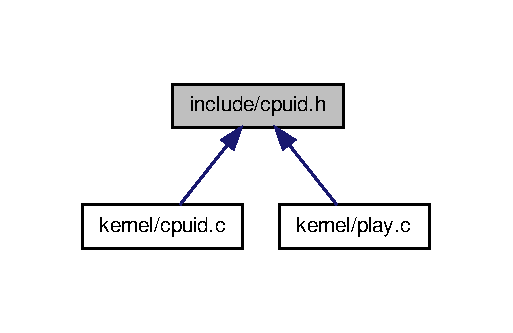
\includegraphics[width=246pt]{cpuid_8h__dep__incl}
\end{center}
\end{figure}
\subsection*{\-Defines}
\begin{DoxyCompactItemize}
\item 
\#define \hyperlink{cpuid_8h_a310fd15487f3d174fe6c3da768a0641a}{\-C\-P\-U\-I\-D\-\_\-\-I\-N\-F\-O}~0x0
\item 
\#define \hyperlink{cpuid_8h_ae7b608851daad3a92c40f0a3c526b27b}{\-C\-P\-U\-I\-D\-\_\-\-V\-E\-R\-S\-I\-O\-N}~0x1
\end{DoxyCompactItemize}


\subsection{\-Define \-Documentation}
\hypertarget{cpuid_8h_a310fd15487f3d174fe6c3da768a0641a}{\index{cpuid.\-h@{cpuid.\-h}!\-C\-P\-U\-I\-D\-\_\-\-I\-N\-F\-O@{\-C\-P\-U\-I\-D\-\_\-\-I\-N\-F\-O}}
\index{\-C\-P\-U\-I\-D\-\_\-\-I\-N\-F\-O@{\-C\-P\-U\-I\-D\-\_\-\-I\-N\-F\-O}!cpuid.h@{cpuid.\-h}}
\subsubsection[{\-C\-P\-U\-I\-D\-\_\-\-I\-N\-F\-O}]{\setlength{\rightskip}{0pt plus 5cm}\#define {\bf \-C\-P\-U\-I\-D\-\_\-\-I\-N\-F\-O}~0x0}}\label{cpuid_8h_a310fd15487f3d174fe6c3da768a0641a}


\-Definition at line 5 of file cpuid.\-h.

\hypertarget{cpuid_8h_ae7b608851daad3a92c40f0a3c526b27b}{\index{cpuid.\-h@{cpuid.\-h}!\-C\-P\-U\-I\-D\-\_\-\-V\-E\-R\-S\-I\-O\-N@{\-C\-P\-U\-I\-D\-\_\-\-V\-E\-R\-S\-I\-O\-N}}
\index{\-C\-P\-U\-I\-D\-\_\-\-V\-E\-R\-S\-I\-O\-N@{\-C\-P\-U\-I\-D\-\_\-\-V\-E\-R\-S\-I\-O\-N}!cpuid.h@{cpuid.\-h}}
\subsubsection[{\-C\-P\-U\-I\-D\-\_\-\-V\-E\-R\-S\-I\-O\-N}]{\setlength{\rightskip}{0pt plus 5cm}\#define {\bf \-C\-P\-U\-I\-D\-\_\-\-V\-E\-R\-S\-I\-O\-N}~0x1}}\label{cpuid_8h_ae7b608851daad3a92c40f0a3c526b27b}


\-Definition at line 6 of file cpuid.\-h.


\hypertarget{device_8h}{\section{include/device.h \-File \-Reference}
\label{device_8h}\index{include/device.\-h@{include/device.\-h}}
}

\hypertarget{ext2fs_8h}{\section{include/fs/ext2fs.h \-File \-Reference}
\label{ext2fs_8h}\index{include/fs/ext2fs.\-h@{include/fs/ext2fs.\-h}}
}
{\ttfamily \#include $<$types.\-h$>$}\*
\-Include dependency graph for ext2fs.\-h\-:\nopagebreak
\begin{figure}[H]
\begin{center}
\leavevmode
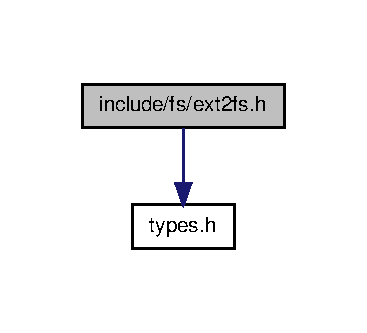
\includegraphics[width=176pt]{ext2fs_8h__incl}
\end{center}
\end{figure}
\subsection*{\-Data \-Structures}
\begin{DoxyCompactItemize}
\item 
struct \hyperlink{structext2__super__block}{ext2\-\_\-super\-\_\-block}
\item 
struct \hyperlink{structext2__dir__entry}{ext2\-\_\-dir\-\_\-entry}
\item 
struct \hyperlink{structext2__group__desc}{ext2\-\_\-group\-\_\-desc}
\item 
struct \hyperlink{structext2__inode}{ext2\-\_\-inode}
\end{DoxyCompactItemize}
\subsection*{\-Defines}
\begin{DoxyCompactItemize}
\item 
\#define \hyperlink{ext2fs_8h_a5466dbceff9b8fe74110eaf7279ac2f8}{\-E\-X\-T2\-\_\-\-N\-D\-I\-R\-\_\-\-B\-L\-O\-C\-K\-S}~12
\item 
\#define \hyperlink{ext2fs_8h_a0ad4fd54bd5dde81d20feca9a9c106c6}{\-E\-X\-T2\-\_\-\-I\-N\-D\-\_\-\-B\-L\-O\-C\-K}~\hyperlink{ext2fs_8h_a5466dbceff9b8fe74110eaf7279ac2f8}{\-E\-X\-T2\-\_\-\-N\-D\-I\-R\-\_\-\-B\-L\-O\-C\-K\-S}
\item 
\#define \hyperlink{ext2fs_8h_a6e95dea120c910dcba3cd94125d5503a}{\-E\-X\-T2\-\_\-\-D\-I\-N\-D\-\_\-\-B\-L\-O\-C\-K}~(\hyperlink{ext2fs_8h_a0ad4fd54bd5dde81d20feca9a9c106c6}{\-E\-X\-T2\-\_\-\-I\-N\-D\-\_\-\-B\-L\-O\-C\-K} + 1)
\item 
\#define \hyperlink{ext2fs_8h_a71858954b55fd2631ea5cba8a33ef1ff}{\-E\-X\-T2\-\_\-\-T\-I\-N\-D\-\_\-\-B\-L\-O\-C\-K}~(\hyperlink{ext2fs_8h_a6e95dea120c910dcba3cd94125d5503a}{\-E\-X\-T2\-\_\-\-D\-I\-N\-D\-\_\-\-B\-L\-O\-C\-K} + 1)
\item 
\#define \hyperlink{ext2fs_8h_add1194efd19a37c1239a967ed68b6614}{\-E\-X\-T2\-\_\-\-N\-\_\-\-B\-L\-O\-C\-K\-S}~(\hyperlink{ext2fs_8h_a71858954b55fd2631ea5cba8a33ef1ff}{\-E\-X\-T2\-\_\-\-T\-I\-N\-D\-\_\-\-B\-L\-O\-C\-K} + 1)
\item 
\#define \hyperlink{ext2fs_8h_a342320971619107a378a494ba58efe62}{\-E\-X\-T2\-\_\-\-I\-N\-O\-S\-Z\-\_\-\-V0}~128
\item 
\#define \hyperlink{ext2fs_8h_a314a7f6544f6f42a028068c0ce164391}{\-E\-X\-T2\-\_\-\-N\-A\-M\-E\-\_\-\-L\-E\-N}~255
\item 
\#define \hyperlink{ext2fs_8h_ae7399e49b7efc3bdef56a903d2e4937e}{\-E\-X\-T2\-\_\-\-C\-L\-E\-A\-N}~1
\item 
\#define \hyperlink{ext2fs_8h_add8802911a5ec1cbdd9aed14115ded7b}{\-E\-X\-T2\-\_\-\-E\-R\-R0\-R}~2
\item 
\#define \hyperlink{ext2fs_8h_a45236cf2faf6b98448760fb49f417e41}{\-E\-X\-T2\-\_\-\-B\-A\-D\-\_\-\-I\-N\-O}~1	/$\ast$ \-Bad blocks inode $\ast$/
\item 
\#define \hyperlink{ext2fs_8h_acb50ee6c9362361d2cc44d8be16f9959}{\-E\-X\-T2\-\_\-\-R\-O\-O\-T\-\_\-\-I\-N\-O}~2	/$\ast$ \-Root inode $\ast$/
\item 
\#define \hyperlink{ext2fs_8h_a855abeeb08fb7aed2778905e1959ef2e}{\-E\-X\-T2\-\_\-\-A\-C\-L\-\_\-\-I\-D\-X\-\_\-\-I\-N\-O}~3	/$\ast$ \-A\-C\-L inode $\ast$/
\item 
\#define \hyperlink{ext2fs_8h_a4463a3f3a2822d8afe7128ac268f232b}{\-E\-X\-T2\-\_\-\-A\-C\-L\-\_\-\-D\-A\-T\-A\-\_\-\-I\-N\-O}~4	/$\ast$ \-A\-C\-L inode $\ast$/
\item 
\#define \hyperlink{ext2fs_8h_a4742bbe5e8b89db8304568b90156c51a}{\-E\-X\-T2\-\_\-\-B\-O\-O\-T\-\_\-\-L\-O\-A\-D\-E\-R\-\_\-\-I\-N\-O}~5	/$\ast$ \-Boot loader inode $\ast$/
\item 
\#define \hyperlink{ext2fs_8h_a56db234c02a3a72218e2cb70131c09e2}{\-E\-X\-T2\-\_\-\-U\-N\-D\-E\-L\-\_\-\-D\-I\-R\-\_\-\-I\-N\-O}~6	/$\ast$ \-Undelete directory inode $\ast$/
\item 
\#define \hyperlink{ext2fs_8h_ac502e094c11b7a93f6b9ac98a08cf1cb}{\-E\-X\-T2\-\_\-\-F\-I\-R\-S\-T\-\_\-\-I\-N\-O}~11	/$\ast$ \-First non reserved inode $\ast$/
\item 
\#define \hyperlink{ext2fs_8h_a34659f525c170d6abdec7e6adea230d1}{\-E\-X\-T2\-\_\-\-P\-R\-E\-\_\-02\-B\-\_\-\-M\-A\-G\-I\-C}~0x\-E\-F51
\item 
\#define \hyperlink{ext2fs_8h_a5a4b87af3f4498e3f2a254e8fbfe2ec3}{\-E\-X\-T2\-\_\-\-S\-U\-P\-E\-R\-\_\-\-M\-A\-G\-I\-C}~0x\-E\-F53
\item 
\#define \hyperlink{ext2fs_8h_a4e09064a0cb2c1e1d6d2c32976acb8a1}{\-E\-X\-T2\-\_\-\-L\-I\-N\-K\-\_\-\-M\-A\-X}~32000
\item 
\#define \hyperlink{ext2fs_8h_a12f28a29b5a657162a64153b8d5ddde2}{\-E\-X\-T2\-\_\-\-I\-G\-N\-O\-R\-E}~1
\item 
\#define \hyperlink{ext2fs_8h_a438f6622e874b6fffb39153204c8ff12}{\-E\-X\-T2\-\_\-\-R\-E\-M\-O\-U\-N\-T\-\_\-\-R\-O}~2
\item 
\#define \hyperlink{ext2fs_8h_a85dbc56d2d2f4dfbf8ebae9fed4ef695}{\-E\-X\-T2\-\_\-\-K\-P\-A\-N\-I\-C}~3
\item 
\#define \hyperlink{ext2fs_8h_a80253adc8e223859f4156fbabb970e32}{\-E\-X\-T2\-\_\-\-O\-S\-\_\-\-L\-I\-N\-U\-X}~0
\item 
\#define \hyperlink{ext2fs_8h_a7af4ecf350d7b5ba9f4d929bc91d4793}{\-E\-X\-T2\-\_\-\-O\-S\-\_\-\-H\-U\-R\-D}~1
\item 
\#define \hyperlink{ext2fs_8h_af9871fe2b6a9510f18263e27ff224f38}{\-E\-X\-T2\-\_\-\-O\-S\-\_\-\-M\-A\-S\-I\-X}~2
\item 
\#define \hyperlink{ext2fs_8h_a244c0e0fc3097187a2ac6a2f5b5f98d9}{\-E\-X\-T2\-\_\-\-O\-S\-\_\-\-F\-B\-S\-D}~3
\item 
\#define \hyperlink{ext2fs_8h_aaf563eacc83118b8d11c7b25bd52d363}{\-E\-X\-T2\-\_\-\-O\-S\-\_\-\-L\-I\-T\-E\-S}~4
\item 
\#define \hyperlink{ext2fs_8h_a5e5d85543e76dc50e70918adcb24201b}{\-E\-X\-T2\-\_\-\-R\-O\-O\-T\-\_\-\-I\-N\-O\-D\-E}~2	/$\ast$ \-Root inode $\ast$/
\item 
\#define \hyperlink{ext2fs_8h_a542ffc63389e10f34d27c87ac0f117de}{\-I\-\_\-\-F\-I\-F\-O}~0x1000
\item 
\#define \hyperlink{ext2fs_8h_aee258b80f48453b5875fdb314e31354c}{\-I\-\_\-\-C\-H\-A\-R\-\_\-\-D\-E\-V\-I\-C\-E}~0x2000
\item 
\#define \hyperlink{ext2fs_8h_a8980abd9f689b9d999b02a6ba2811271}{\-I\-\_\-\-D\-I\-R\-E\-C\-T\-O\-R\-Y}~0x4000
\item 
\#define \hyperlink{ext2fs_8h_a99e0d67edb6a60f5a9279342afd3132e}{\-I\-\_\-\-B\-L\-O\-C\-K\-\_\-\-D\-E\-V\-I\-C\-E}~0x6000
\item 
\#define \hyperlink{ext2fs_8h_a75473feabda8cf4b780b3da60bbdfa73}{\-I\-\_\-\-R\-E\-G\-\_\-\-F\-I\-L\-E}~0x8000
\item 
\#define \hyperlink{ext2fs_8h_adcce939418387c9825733557a76498fb}{\-I\-\_\-\-S\-Y\-M\-\_\-\-L\-I\-N\-K}~0x\-A000
\item 
\#define \hyperlink{ext2fs_8h_ac5ada9f0953aa7af119d49f75fa56e7e}{\-I\-\_\-\-U\-N\-I\-X\-\_\-\-S\-O\-C\-K}~0x\-C000
\item 
\#define \hyperlink{ext2fs_8h_a75a14467c538f136fe238c24689c9677}{\-I\-\_\-\-O\-E\-X\-E\-C\-\_\-\-P}~0\-X001
\item 
\#define \hyperlink{ext2fs_8h_aebdc994096b363323d0685417acb40b3}{\-I\-\_\-\-O\-W\-R\-I\-T\-E\-\_\-\-P}~0x002
\item 
\#define \hyperlink{ext2fs_8h_a90f85ce3d29d5f0537ee98cee5fe8dc2}{\-I\-\_\-\-O\-R\-E\-A\-D\-\_\-\-P}~0x004
\item 
\#define \hyperlink{ext2fs_8h_aec5106a6d4af3b05a6b6c2d5ca9f1757}{\-I\-\_\-\-G\-E\-X\-E\-C\-\_\-\-P}~0x008
\item 
\#define \hyperlink{ext2fs_8h_a62585f055450f5cfb051121163b3042b}{\-I\-\_\-\-G\-W\-R\-I\-T\-E\-\_\-\-P}~0x010
\item 
\#define \hyperlink{ext2fs_8h_a3a1c6a7d064ee00054c4943604477618}{\-I\-\_\-\-G\-R\-E\-A\-D\-\_\-\-P}~0x020
\item 
\#define \hyperlink{ext2fs_8h_a3f28fbb058b04cc0b7ddc034a92f508f}{\-I\-\_\-\-U\-E\-X\-E\-C\-\_\-\-P}~0x040
\item 
\#define \hyperlink{ext2fs_8h_a562dd09ffc3ad51913925317e2c10bc7}{\-I\-\_\-\-U\-W\-R\-I\-T\-E\-\_\-\-P}~0x080
\item 
\#define \hyperlink{ext2fs_8h_abaa2200bba98d5778c6a50d2b9a95d60}{\-I\-\_\-\-U\-R\-E\-A\-D\-\_\-\-P}~0x100
\item 
\#define \hyperlink{ext2fs_8h_ae8295105ca5fe1bc327f884539499cf6}{\-I\-\_\-\-S\-T\-I\-C\-K\-Y}~0x200
\item 
\#define \hyperlink{ext2fs_8h_abfe1f88ff55c94639b4289cc95eed80c}{\-I\-\_\-\-S\-E\-T\-\_\-\-G\-I\-D}~0x400
\item 
\#define \hyperlink{ext2fs_8h_aea12b910ed271583a1b559f087a1ed2d}{\-I\-\_\-\-S\-E\-T\-\_\-\-U\-I\-D}~0x800
\item 
\#define \hyperlink{ext2fs_8h_a1ef3c72b3ef7ec790f2ac2d51e64e235}{\-I\-\_\-\-S\-E\-C\-\_\-\-D\-E\-L}~0x00000001  /$\ast$\-Secure deletion$\ast$/
\item 
\#define \hyperlink{ext2fs_8h_a362b42c224039fa757d5f14dddb4cace}{\-I\-\_\-\-K\-E\-E\-P\-\_\-\-C\-P\-Y}~0x00000002  /$\ast$\-Keep a copy of data when deleted$\ast$/
\item 
\#define \hyperlink{ext2fs_8h_a1c780125164b5b272f82985cfcc15667}{\-I\-\_\-\-F\-I\-L\-E\-\_\-\-C\-O\-M\-P\-R\-E\-S\-S\-I\-O\-N}~0x00000004  /$\ast$\-File compression$\ast$/
\item 
\#define \hyperlink{ext2fs_8h_ae7e8ddd594fbe81343210eb4e3f83519}{\-I\-\_\-\-S\-Y\-N\-C\-\_\-\-U\-P\-D\-A\-T\-E\-S}~0x00000008  /$\ast$\-Synchronous updates$\ast$/
\item 
\#define \hyperlink{ext2fs_8h_aaed1f8e0b6f4a64dcc057cd30aab7082}{\-I\-\_\-\-I\-M\-M\-U\-T\-A\-B\-L\-E\-\_\-\-F\-I\-L\-E}~0x00000010  /$\ast$\-Immutable file$\ast$/
\item 
\#define \hyperlink{ext2fs_8h_a437bbe574a661f9f29531654f925458b}{\-I\-\_\-\-A\-P\-P\-E\-N\-D\-\_\-\-O\-N\-L\-Y}~0x00000020  /$\ast$ Append only $\ast$/
\item 
\#define \hyperlink{ext2fs_8h_af2e90ad39b34a55acbd05e420c3a1548}{\-I\-\_\-\-N\-O\-\_\-\-D\-U\-M\-P}~0x00000040  /$\ast$ File is not included in 'dump' command $\ast$/
\item 
\#define \hyperlink{ext2fs_8h_a8680369aaead46148826f8830378c0c0}{\-I\-\_\-\-N\-O\-\_\-\-L\-A\-T}~0x00000080  /$\ast$ Last accessed time should not updated $\ast$/
\item 
\#define \hyperlink{ext2fs_8h_a26c041da95bb78e5d94afbf5bb792201}{\-I\-\_\-\-H\-A\-S\-H\-\_\-\-I\-N\-D\-E\-X\-E\-D\-\_\-\-D\-I\-R}~0x00010000  /$\ast$ Hash indexed directory $\ast$/
\item 
\#define \hyperlink{ext2fs_8h_ab1d5bb39a0f63f443c0ea1947d45487a}{\-I\-\_\-\-A\-F\-S\-\_\-\-D\-I\-R}~0x00020000  /$\ast$ A\-F\-S directory $\ast$/
\item 
\#define \hyperlink{ext2fs_8h_a5033e488424488d0b68524e04c4687d4}{\-I\-\_\-\-J\-O\-U\-R\-N\-A\-L\-\_\-\-F\-I\-L\-E\-\_\-\-D\-A\-T\-A}~0x00040000  /$\ast$ Journal file data $\ast$/
\item 
\#define \hyperlink{ext2fs_8h_ac3344d402895bc2e1b2a484e0b53b42e}{\-I\-\_\-\-D\-I\-R\-\_\-\-U\-N\-K\-O\-W\-N}~0x0
\item 
\#define \hyperlink{ext2fs_8h_aa97f9ed1f26bbdb2e6571eecad0043d5}{\-I\-\_\-\-D\-I\-R\-\_\-\-R\-E\-G\-U\-L\-A\-R\-\_\-\-F}~0x1
\item 
\#define \hyperlink{ext2fs_8h_aee4eb0da717fa9fd5a6af3bca3cceddb}{\-I\-\_\-\-D\-I\-R\-\_\-\-D\-I\-R\-E\-C\-T\-O\-R\-Y}~0x2
\item 
\#define \hyperlink{ext2fs_8h_a48258119f9033b605e8e2a5aadb14037}{\-I\-\_\-\-D\-I\-R\-\_\-\-C\-H\-A\-R\-\_\-\-D\-E\-V}~0x3
\item 
\#define \hyperlink{ext2fs_8h_a4b0417c1233ca7e0f696bae123a57690}{\-I\-\_\-\-D\-I\-R\-\_\-\-B\-L\-O\-C\-K\-\_\-\-D\-E\-V}~0x4
\item 
\#define \hyperlink{ext2fs_8h_ab76198e6d38cda1758b6b1e3f49d8cc8}{\-I\-\_\-\-D\-I\-R\-\_\-\-F\-I\-F\-O}~0x5
\item 
\#define \hyperlink{ext2fs_8h_a2743ed6716937ccea9283778ac4e5999}{\-I\-\_\-\-D\-I\-R\-\_\-\-S\-O\-C\-K}~0x6
\item 
\#define \hyperlink{ext2fs_8h_a1e07ec0a2a7ac5ce09becc7858333091}{\-I\-\_\-\-D\-I\-R\-\_\-\-S\-Y\-M\-\_\-\-L\-I\-N\-K}~0x7
\item 
\#define \hyperlink{ext2fs_8h_ab6162564500fa3317fd74957ef03262a}{\-E\-X\-T2\-\_\-\-P\-R\-E\-L\-O\-C}~0x0001
\item 
\#define \hyperlink{ext2fs_8h_add8f4cc7c4d100e712ab1c8d5e4be97f}{\-E\-X\-T2\-\_\-\-A\-F\-S\-\_\-\-I\-N\-O}~0x0002
\item 
\#define \hyperlink{ext2fs_8h_a2439f1429bea87a618cad37d47fc54fd}{\-E\-X\-T2\-\_\-\-J\-R\-N\-L}~0x0004
\item 
\#define \hyperlink{ext2fs_8h_ac77c305d8e8aa7f02ee80bdf41fa9f1e}{\-E\-X\-T2\-\_\-\-I\-N\-O\-\_\-\-E\-X\-T\-N\-D\-A\-T\-T\-R}~0x0008
\item 
\#define \hyperlink{ext2fs_8h_a35e8e8d3e9006398c725177b30247b7e}{\-E\-X\-T2\-\_\-\-F\-S\-\_\-\-R\-E\-S\-I\-Z\-E}~0x0010
\item 
\#define \hyperlink{ext2fs_8h_ac9456c1ce959993d394b624cc3a7414f}{\-E\-X\-T2\-\_\-\-D\-I\-R\-\_\-\-H\-A\-S\-H\-I}~0x0020
\item 
\#define \hyperlink{ext2fs_8h_ab38129c0dec55ae2b8666649cf893113}{\-E\-X\-T2\-\_\-\-C\-O\-M\-P\-R\-E\-S\-S\-I\-O\-N}~0x0001
\item 
\#define \hyperlink{ext2fs_8h_ae7e710692796e837afbeb0133613aa41}{\-E\-X\-T2\-\_\-\-D\-I\-R\-\_\-\-T\-Y\-P\-E\-\_\-\-F}~0x0002
\item 
\#define \hyperlink{ext2fs_8h_a5076caf4d12e7a1c874649077d214ce9}{\-E\-X\-T2\-\_\-\-F\-S\-\_\-\-R\-E\-P\-L\-A\-Y\-\_\-\-J\-O\-R}~0x0004
\item 
\#define \hyperlink{ext2fs_8h_a8f5bc740655a9480742cc4333269f58c}{\-E\-X\-T2\-\_\-\-F\-S\-\_\-\-J\-O\-R\-\_\-\-D\-E\-V}~0x0008
\item 
\#define \hyperlink{ext2fs_8h_a47357b3a4baf8c32e6c6db9a0197dd7e}{\-E\-X\-T2\-\_\-\-S\-P\-A\-R\-S\-E}~0x0001
\item 
\#define \hyperlink{ext2fs_8h_a8105cd2c5ca3068570afed5497179d97}{\-E\-X\-T2\-\_\-64\-F\-Z}~0x0002
\item 
\#define \hyperlink{ext2fs_8h_a67767224a3161076e9e8c061f5054587}{\-E\-X\-T2\-\_\-\-D\-I\-R\-\_\-\-B\-I\-N\-\_\-\-T\-R\-E\-E}~0x0004
\end{DoxyCompactItemize}


\subsection{\-Define \-Documentation}
\hypertarget{ext2fs_8h_a8105cd2c5ca3068570afed5497179d97}{\index{ext2fs.\-h@{ext2fs.\-h}!\-E\-X\-T2\-\_\-64\-F\-Z@{\-E\-X\-T2\-\_\-64\-F\-Z}}
\index{\-E\-X\-T2\-\_\-64\-F\-Z@{\-E\-X\-T2\-\_\-64\-F\-Z}!ext2fs.h@{ext2fs.\-h}}
\subsubsection[{\-E\-X\-T2\-\_\-64\-F\-Z}]{\setlength{\rightskip}{0pt plus 5cm}\#define {\bf \-E\-X\-T2\-\_\-64\-F\-Z}~0x0002}}\label{ext2fs_8h_a8105cd2c5ca3068570afed5497179d97}


\-Definition at line 114 of file ext2fs.\-h.

\hypertarget{ext2fs_8h_a4463a3f3a2822d8afe7128ac268f232b}{\index{ext2fs.\-h@{ext2fs.\-h}!\-E\-X\-T2\-\_\-\-A\-C\-L\-\_\-\-D\-A\-T\-A\-\_\-\-I\-N\-O@{\-E\-X\-T2\-\_\-\-A\-C\-L\-\_\-\-D\-A\-T\-A\-\_\-\-I\-N\-O}}
\index{\-E\-X\-T2\-\_\-\-A\-C\-L\-\_\-\-D\-A\-T\-A\-\_\-\-I\-N\-O@{\-E\-X\-T2\-\_\-\-A\-C\-L\-\_\-\-D\-A\-T\-A\-\_\-\-I\-N\-O}!ext2fs.h@{ext2fs.\-h}}
\subsubsection[{\-E\-X\-T2\-\_\-\-A\-C\-L\-\_\-\-D\-A\-T\-A\-\_\-\-I\-N\-O}]{\setlength{\rightskip}{0pt plus 5cm}\#define {\bf \-E\-X\-T2\-\_\-\-A\-C\-L\-\_\-\-D\-A\-T\-A\-\_\-\-I\-N\-O}~4	/$\ast$ \-A\-C\-L inode $\ast$/}}\label{ext2fs_8h_a4463a3f3a2822d8afe7128ac268f232b}


\-Definition at line 23 of file ext2fs.\-h.

\hypertarget{ext2fs_8h_a855abeeb08fb7aed2778905e1959ef2e}{\index{ext2fs.\-h@{ext2fs.\-h}!\-E\-X\-T2\-\_\-\-A\-C\-L\-\_\-\-I\-D\-X\-\_\-\-I\-N\-O@{\-E\-X\-T2\-\_\-\-A\-C\-L\-\_\-\-I\-D\-X\-\_\-\-I\-N\-O}}
\index{\-E\-X\-T2\-\_\-\-A\-C\-L\-\_\-\-I\-D\-X\-\_\-\-I\-N\-O@{\-E\-X\-T2\-\_\-\-A\-C\-L\-\_\-\-I\-D\-X\-\_\-\-I\-N\-O}!ext2fs.h@{ext2fs.\-h}}
\subsubsection[{\-E\-X\-T2\-\_\-\-A\-C\-L\-\_\-\-I\-D\-X\-\_\-\-I\-N\-O}]{\setlength{\rightskip}{0pt plus 5cm}\#define {\bf \-E\-X\-T2\-\_\-\-A\-C\-L\-\_\-\-I\-D\-X\-\_\-\-I\-N\-O}~3	/$\ast$ \-A\-C\-L inode $\ast$/}}\label{ext2fs_8h_a855abeeb08fb7aed2778905e1959ef2e}


\-Definition at line 22 of file ext2fs.\-h.

\hypertarget{ext2fs_8h_add8f4cc7c4d100e712ab1c8d5e4be97f}{\index{ext2fs.\-h@{ext2fs.\-h}!\-E\-X\-T2\-\_\-\-A\-F\-S\-\_\-\-I\-N\-O@{\-E\-X\-T2\-\_\-\-A\-F\-S\-\_\-\-I\-N\-O}}
\index{\-E\-X\-T2\-\_\-\-A\-F\-S\-\_\-\-I\-N\-O@{\-E\-X\-T2\-\_\-\-A\-F\-S\-\_\-\-I\-N\-O}!ext2fs.h@{ext2fs.\-h}}
\subsubsection[{\-E\-X\-T2\-\_\-\-A\-F\-S\-\_\-\-I\-N\-O}]{\setlength{\rightskip}{0pt plus 5cm}\#define {\bf \-E\-X\-T2\-\_\-\-A\-F\-S\-\_\-\-I\-N\-O}~0x0002}}\label{ext2fs_8h_add8f4cc7c4d100e712ab1c8d5e4be97f}


\-Definition at line 102 of file ext2fs.\-h.

\hypertarget{ext2fs_8h_a45236cf2faf6b98448760fb49f417e41}{\index{ext2fs.\-h@{ext2fs.\-h}!\-E\-X\-T2\-\_\-\-B\-A\-D\-\_\-\-I\-N\-O@{\-E\-X\-T2\-\_\-\-B\-A\-D\-\_\-\-I\-N\-O}}
\index{\-E\-X\-T2\-\_\-\-B\-A\-D\-\_\-\-I\-N\-O@{\-E\-X\-T2\-\_\-\-B\-A\-D\-\_\-\-I\-N\-O}!ext2fs.h@{ext2fs.\-h}}
\subsubsection[{\-E\-X\-T2\-\_\-\-B\-A\-D\-\_\-\-I\-N\-O}]{\setlength{\rightskip}{0pt plus 5cm}\#define {\bf \-E\-X\-T2\-\_\-\-B\-A\-D\-\_\-\-I\-N\-O}~1	/$\ast$ \-Bad blocks inode $\ast$/}}\label{ext2fs_8h_a45236cf2faf6b98448760fb49f417e41}


\-Definition at line 20 of file ext2fs.\-h.

\hypertarget{ext2fs_8h_a4742bbe5e8b89db8304568b90156c51a}{\index{ext2fs.\-h@{ext2fs.\-h}!\-E\-X\-T2\-\_\-\-B\-O\-O\-T\-\_\-\-L\-O\-A\-D\-E\-R\-\_\-\-I\-N\-O@{\-E\-X\-T2\-\_\-\-B\-O\-O\-T\-\_\-\-L\-O\-A\-D\-E\-R\-\_\-\-I\-N\-O}}
\index{\-E\-X\-T2\-\_\-\-B\-O\-O\-T\-\_\-\-L\-O\-A\-D\-E\-R\-\_\-\-I\-N\-O@{\-E\-X\-T2\-\_\-\-B\-O\-O\-T\-\_\-\-L\-O\-A\-D\-E\-R\-\_\-\-I\-N\-O}!ext2fs.h@{ext2fs.\-h}}
\subsubsection[{\-E\-X\-T2\-\_\-\-B\-O\-O\-T\-\_\-\-L\-O\-A\-D\-E\-R\-\_\-\-I\-N\-O}]{\setlength{\rightskip}{0pt plus 5cm}\#define {\bf \-E\-X\-T2\-\_\-\-B\-O\-O\-T\-\_\-\-L\-O\-A\-D\-E\-R\-\_\-\-I\-N\-O}~5	/$\ast$ \-Boot loader inode $\ast$/}}\label{ext2fs_8h_a4742bbe5e8b89db8304568b90156c51a}


\-Definition at line 24 of file ext2fs.\-h.

\hypertarget{ext2fs_8h_ae7399e49b7efc3bdef56a903d2e4937e}{\index{ext2fs.\-h@{ext2fs.\-h}!\-E\-X\-T2\-\_\-\-C\-L\-E\-A\-N@{\-E\-X\-T2\-\_\-\-C\-L\-E\-A\-N}}
\index{\-E\-X\-T2\-\_\-\-C\-L\-E\-A\-N@{\-E\-X\-T2\-\_\-\-C\-L\-E\-A\-N}!ext2fs.h@{ext2fs.\-h}}
\subsubsection[{\-E\-X\-T2\-\_\-\-C\-L\-E\-A\-N}]{\setlength{\rightskip}{0pt plus 5cm}\#define {\bf \-E\-X\-T2\-\_\-\-C\-L\-E\-A\-N}~1}}\label{ext2fs_8h_ae7399e49b7efc3bdef56a903d2e4937e}


\-Definition at line 15 of file ext2fs.\-h.

\hypertarget{ext2fs_8h_ab38129c0dec55ae2b8666649cf893113}{\index{ext2fs.\-h@{ext2fs.\-h}!\-E\-X\-T2\-\_\-\-C\-O\-M\-P\-R\-E\-S\-S\-I\-O\-N@{\-E\-X\-T2\-\_\-\-C\-O\-M\-P\-R\-E\-S\-S\-I\-O\-N}}
\index{\-E\-X\-T2\-\_\-\-C\-O\-M\-P\-R\-E\-S\-S\-I\-O\-N@{\-E\-X\-T2\-\_\-\-C\-O\-M\-P\-R\-E\-S\-S\-I\-O\-N}!ext2fs.h@{ext2fs.\-h}}
\subsubsection[{\-E\-X\-T2\-\_\-\-C\-O\-M\-P\-R\-E\-S\-S\-I\-O\-N}]{\setlength{\rightskip}{0pt plus 5cm}\#define {\bf \-E\-X\-T2\-\_\-\-C\-O\-M\-P\-R\-E\-S\-S\-I\-O\-N}~0x0001}}\label{ext2fs_8h_ab38129c0dec55ae2b8666649cf893113}


\-Definition at line 108 of file ext2fs.\-h.

\hypertarget{ext2fs_8h_a6e95dea120c910dcba3cd94125d5503a}{\index{ext2fs.\-h@{ext2fs.\-h}!\-E\-X\-T2\-\_\-\-D\-I\-N\-D\-\_\-\-B\-L\-O\-C\-K@{\-E\-X\-T2\-\_\-\-D\-I\-N\-D\-\_\-\-B\-L\-O\-C\-K}}
\index{\-E\-X\-T2\-\_\-\-D\-I\-N\-D\-\_\-\-B\-L\-O\-C\-K@{\-E\-X\-T2\-\_\-\-D\-I\-N\-D\-\_\-\-B\-L\-O\-C\-K}!ext2fs.h@{ext2fs.\-h}}
\subsubsection[{\-E\-X\-T2\-\_\-\-D\-I\-N\-D\-\_\-\-B\-L\-O\-C\-K}]{\setlength{\rightskip}{0pt plus 5cm}\#define {\bf \-E\-X\-T2\-\_\-\-D\-I\-N\-D\-\_\-\-B\-L\-O\-C\-K}~({\bf \-E\-X\-T2\-\_\-\-I\-N\-D\-\_\-\-B\-L\-O\-C\-K} + 1)}}\label{ext2fs_8h_a6e95dea120c910dcba3cd94125d5503a}


\-Definition at line 9 of file ext2fs.\-h.

\hypertarget{ext2fs_8h_a67767224a3161076e9e8c061f5054587}{\index{ext2fs.\-h@{ext2fs.\-h}!\-E\-X\-T2\-\_\-\-D\-I\-R\-\_\-\-B\-I\-N\-\_\-\-T\-R\-E\-E@{\-E\-X\-T2\-\_\-\-D\-I\-R\-\_\-\-B\-I\-N\-\_\-\-T\-R\-E\-E}}
\index{\-E\-X\-T2\-\_\-\-D\-I\-R\-\_\-\-B\-I\-N\-\_\-\-T\-R\-E\-E@{\-E\-X\-T2\-\_\-\-D\-I\-R\-\_\-\-B\-I\-N\-\_\-\-T\-R\-E\-E}!ext2fs.h@{ext2fs.\-h}}
\subsubsection[{\-E\-X\-T2\-\_\-\-D\-I\-R\-\_\-\-B\-I\-N\-\_\-\-T\-R\-E\-E}]{\setlength{\rightskip}{0pt plus 5cm}\#define {\bf \-E\-X\-T2\-\_\-\-D\-I\-R\-\_\-\-B\-I\-N\-\_\-\-T\-R\-E\-E}~0x0004}}\label{ext2fs_8h_a67767224a3161076e9e8c061f5054587}


\-Definition at line 115 of file ext2fs.\-h.

\hypertarget{ext2fs_8h_ac9456c1ce959993d394b624cc3a7414f}{\index{ext2fs.\-h@{ext2fs.\-h}!\-E\-X\-T2\-\_\-\-D\-I\-R\-\_\-\-H\-A\-S\-H\-I@{\-E\-X\-T2\-\_\-\-D\-I\-R\-\_\-\-H\-A\-S\-H\-I}}
\index{\-E\-X\-T2\-\_\-\-D\-I\-R\-\_\-\-H\-A\-S\-H\-I@{\-E\-X\-T2\-\_\-\-D\-I\-R\-\_\-\-H\-A\-S\-H\-I}!ext2fs.h@{ext2fs.\-h}}
\subsubsection[{\-E\-X\-T2\-\_\-\-D\-I\-R\-\_\-\-H\-A\-S\-H\-I}]{\setlength{\rightskip}{0pt plus 5cm}\#define {\bf \-E\-X\-T2\-\_\-\-D\-I\-R\-\_\-\-H\-A\-S\-H\-I}~0x0020}}\label{ext2fs_8h_ac9456c1ce959993d394b624cc3a7414f}


\-Definition at line 106 of file ext2fs.\-h.

\hypertarget{ext2fs_8h_ae7e710692796e837afbeb0133613aa41}{\index{ext2fs.\-h@{ext2fs.\-h}!\-E\-X\-T2\-\_\-\-D\-I\-R\-\_\-\-T\-Y\-P\-E\-\_\-\-F@{\-E\-X\-T2\-\_\-\-D\-I\-R\-\_\-\-T\-Y\-P\-E\-\_\-\-F}}
\index{\-E\-X\-T2\-\_\-\-D\-I\-R\-\_\-\-T\-Y\-P\-E\-\_\-\-F@{\-E\-X\-T2\-\_\-\-D\-I\-R\-\_\-\-T\-Y\-P\-E\-\_\-\-F}!ext2fs.h@{ext2fs.\-h}}
\subsubsection[{\-E\-X\-T2\-\_\-\-D\-I\-R\-\_\-\-T\-Y\-P\-E\-\_\-\-F}]{\setlength{\rightskip}{0pt plus 5cm}\#define {\bf \-E\-X\-T2\-\_\-\-D\-I\-R\-\_\-\-T\-Y\-P\-E\-\_\-\-F}~0x0002}}\label{ext2fs_8h_ae7e710692796e837afbeb0133613aa41}


\-Definition at line 109 of file ext2fs.\-h.

\hypertarget{ext2fs_8h_add8802911a5ec1cbdd9aed14115ded7b}{\index{ext2fs.\-h@{ext2fs.\-h}!\-E\-X\-T2\-\_\-\-E\-R\-R0\-R@{\-E\-X\-T2\-\_\-\-E\-R\-R0\-R}}
\index{\-E\-X\-T2\-\_\-\-E\-R\-R0\-R@{\-E\-X\-T2\-\_\-\-E\-R\-R0\-R}!ext2fs.h@{ext2fs.\-h}}
\subsubsection[{\-E\-X\-T2\-\_\-\-E\-R\-R0\-R}]{\setlength{\rightskip}{0pt plus 5cm}\#define {\bf \-E\-X\-T2\-\_\-\-E\-R\-R0\-R}~2}}\label{ext2fs_8h_add8802911a5ec1cbdd9aed14115ded7b}


\-Definition at line 16 of file ext2fs.\-h.

\hypertarget{ext2fs_8h_ac502e094c11b7a93f6b9ac98a08cf1cb}{\index{ext2fs.\-h@{ext2fs.\-h}!\-E\-X\-T2\-\_\-\-F\-I\-R\-S\-T\-\_\-\-I\-N\-O@{\-E\-X\-T2\-\_\-\-F\-I\-R\-S\-T\-\_\-\-I\-N\-O}}
\index{\-E\-X\-T2\-\_\-\-F\-I\-R\-S\-T\-\_\-\-I\-N\-O@{\-E\-X\-T2\-\_\-\-F\-I\-R\-S\-T\-\_\-\-I\-N\-O}!ext2fs.h@{ext2fs.\-h}}
\subsubsection[{\-E\-X\-T2\-\_\-\-F\-I\-R\-S\-T\-\_\-\-I\-N\-O}]{\setlength{\rightskip}{0pt plus 5cm}\#define {\bf \-E\-X\-T2\-\_\-\-F\-I\-R\-S\-T\-\_\-\-I\-N\-O}~11	/$\ast$ \-First non reserved inode $\ast$/}}\label{ext2fs_8h_ac502e094c11b7a93f6b9ac98a08cf1cb}


\-Definition at line 26 of file ext2fs.\-h.

\hypertarget{ext2fs_8h_a8f5bc740655a9480742cc4333269f58c}{\index{ext2fs.\-h@{ext2fs.\-h}!\-E\-X\-T2\-\_\-\-F\-S\-\_\-\-J\-O\-R\-\_\-\-D\-E\-V@{\-E\-X\-T2\-\_\-\-F\-S\-\_\-\-J\-O\-R\-\_\-\-D\-E\-V}}
\index{\-E\-X\-T2\-\_\-\-F\-S\-\_\-\-J\-O\-R\-\_\-\-D\-E\-V@{\-E\-X\-T2\-\_\-\-F\-S\-\_\-\-J\-O\-R\-\_\-\-D\-E\-V}!ext2fs.h@{ext2fs.\-h}}
\subsubsection[{\-E\-X\-T2\-\_\-\-F\-S\-\_\-\-J\-O\-R\-\_\-\-D\-E\-V}]{\setlength{\rightskip}{0pt plus 5cm}\#define {\bf \-E\-X\-T2\-\_\-\-F\-S\-\_\-\-J\-O\-R\-\_\-\-D\-E\-V}~0x0008}}\label{ext2fs_8h_a8f5bc740655a9480742cc4333269f58c}


\-Definition at line 111 of file ext2fs.\-h.

\hypertarget{ext2fs_8h_a5076caf4d12e7a1c874649077d214ce9}{\index{ext2fs.\-h@{ext2fs.\-h}!\-E\-X\-T2\-\_\-\-F\-S\-\_\-\-R\-E\-P\-L\-A\-Y\-\_\-\-J\-O\-R@{\-E\-X\-T2\-\_\-\-F\-S\-\_\-\-R\-E\-P\-L\-A\-Y\-\_\-\-J\-O\-R}}
\index{\-E\-X\-T2\-\_\-\-F\-S\-\_\-\-R\-E\-P\-L\-A\-Y\-\_\-\-J\-O\-R@{\-E\-X\-T2\-\_\-\-F\-S\-\_\-\-R\-E\-P\-L\-A\-Y\-\_\-\-J\-O\-R}!ext2fs.h@{ext2fs.\-h}}
\subsubsection[{\-E\-X\-T2\-\_\-\-F\-S\-\_\-\-R\-E\-P\-L\-A\-Y\-\_\-\-J\-O\-R}]{\setlength{\rightskip}{0pt plus 5cm}\#define {\bf \-E\-X\-T2\-\_\-\-F\-S\-\_\-\-R\-E\-P\-L\-A\-Y\-\_\-\-J\-O\-R}~0x0004}}\label{ext2fs_8h_a5076caf4d12e7a1c874649077d214ce9}


\-Definition at line 110 of file ext2fs.\-h.

\hypertarget{ext2fs_8h_a35e8e8d3e9006398c725177b30247b7e}{\index{ext2fs.\-h@{ext2fs.\-h}!\-E\-X\-T2\-\_\-\-F\-S\-\_\-\-R\-E\-S\-I\-Z\-E@{\-E\-X\-T2\-\_\-\-F\-S\-\_\-\-R\-E\-S\-I\-Z\-E}}
\index{\-E\-X\-T2\-\_\-\-F\-S\-\_\-\-R\-E\-S\-I\-Z\-E@{\-E\-X\-T2\-\_\-\-F\-S\-\_\-\-R\-E\-S\-I\-Z\-E}!ext2fs.h@{ext2fs.\-h}}
\subsubsection[{\-E\-X\-T2\-\_\-\-F\-S\-\_\-\-R\-E\-S\-I\-Z\-E}]{\setlength{\rightskip}{0pt plus 5cm}\#define {\bf \-E\-X\-T2\-\_\-\-F\-S\-\_\-\-R\-E\-S\-I\-Z\-E}~0x0010}}\label{ext2fs_8h_a35e8e8d3e9006398c725177b30247b7e}


\-Definition at line 105 of file ext2fs.\-h.

\hypertarget{ext2fs_8h_a12f28a29b5a657162a64153b8d5ddde2}{\index{ext2fs.\-h@{ext2fs.\-h}!\-E\-X\-T2\-\_\-\-I\-G\-N\-O\-R\-E@{\-E\-X\-T2\-\_\-\-I\-G\-N\-O\-R\-E}}
\index{\-E\-X\-T2\-\_\-\-I\-G\-N\-O\-R\-E@{\-E\-X\-T2\-\_\-\-I\-G\-N\-O\-R\-E}!ext2fs.h@{ext2fs.\-h}}
\subsubsection[{\-E\-X\-T2\-\_\-\-I\-G\-N\-O\-R\-E}]{\setlength{\rightskip}{0pt plus 5cm}\#define {\bf \-E\-X\-T2\-\_\-\-I\-G\-N\-O\-R\-E}~1}}\label{ext2fs_8h_a12f28a29b5a657162a64153b8d5ddde2}


\-Definition at line 40 of file ext2fs.\-h.

\hypertarget{ext2fs_8h_a0ad4fd54bd5dde81d20feca9a9c106c6}{\index{ext2fs.\-h@{ext2fs.\-h}!\-E\-X\-T2\-\_\-\-I\-N\-D\-\_\-\-B\-L\-O\-C\-K@{\-E\-X\-T2\-\_\-\-I\-N\-D\-\_\-\-B\-L\-O\-C\-K}}
\index{\-E\-X\-T2\-\_\-\-I\-N\-D\-\_\-\-B\-L\-O\-C\-K@{\-E\-X\-T2\-\_\-\-I\-N\-D\-\_\-\-B\-L\-O\-C\-K}!ext2fs.h@{ext2fs.\-h}}
\subsubsection[{\-E\-X\-T2\-\_\-\-I\-N\-D\-\_\-\-B\-L\-O\-C\-K}]{\setlength{\rightskip}{0pt plus 5cm}\#define {\bf \-E\-X\-T2\-\_\-\-I\-N\-D\-\_\-\-B\-L\-O\-C\-K}~{\bf \-E\-X\-T2\-\_\-\-N\-D\-I\-R\-\_\-\-B\-L\-O\-C\-K\-S}}}\label{ext2fs_8h_a0ad4fd54bd5dde81d20feca9a9c106c6}


\-Definition at line 8 of file ext2fs.\-h.

\hypertarget{ext2fs_8h_ac77c305d8e8aa7f02ee80bdf41fa9f1e}{\index{ext2fs.\-h@{ext2fs.\-h}!\-E\-X\-T2\-\_\-\-I\-N\-O\-\_\-\-E\-X\-T\-N\-D\-A\-T\-T\-R@{\-E\-X\-T2\-\_\-\-I\-N\-O\-\_\-\-E\-X\-T\-N\-D\-A\-T\-T\-R}}
\index{\-E\-X\-T2\-\_\-\-I\-N\-O\-\_\-\-E\-X\-T\-N\-D\-A\-T\-T\-R@{\-E\-X\-T2\-\_\-\-I\-N\-O\-\_\-\-E\-X\-T\-N\-D\-A\-T\-T\-R}!ext2fs.h@{ext2fs.\-h}}
\subsubsection[{\-E\-X\-T2\-\_\-\-I\-N\-O\-\_\-\-E\-X\-T\-N\-D\-A\-T\-T\-R}]{\setlength{\rightskip}{0pt plus 5cm}\#define {\bf \-E\-X\-T2\-\_\-\-I\-N\-O\-\_\-\-E\-X\-T\-N\-D\-A\-T\-T\-R}~0x0008}}\label{ext2fs_8h_ac77c305d8e8aa7f02ee80bdf41fa9f1e}


\-Definition at line 104 of file ext2fs.\-h.

\hypertarget{ext2fs_8h_a342320971619107a378a494ba58efe62}{\index{ext2fs.\-h@{ext2fs.\-h}!\-E\-X\-T2\-\_\-\-I\-N\-O\-S\-Z\-\_\-\-V0@{\-E\-X\-T2\-\_\-\-I\-N\-O\-S\-Z\-\_\-\-V0}}
\index{\-E\-X\-T2\-\_\-\-I\-N\-O\-S\-Z\-\_\-\-V0@{\-E\-X\-T2\-\_\-\-I\-N\-O\-S\-Z\-\_\-\-V0}!ext2fs.h@{ext2fs.\-h}}
\subsubsection[{\-E\-X\-T2\-\_\-\-I\-N\-O\-S\-Z\-\_\-\-V0}]{\setlength{\rightskip}{0pt plus 5cm}\#define {\bf \-E\-X\-T2\-\_\-\-I\-N\-O\-S\-Z\-\_\-\-V0}~128}}\label{ext2fs_8h_a342320971619107a378a494ba58efe62}


\-Definition at line 12 of file ext2fs.\-h.

\hypertarget{ext2fs_8h_a2439f1429bea87a618cad37d47fc54fd}{\index{ext2fs.\-h@{ext2fs.\-h}!\-E\-X\-T2\-\_\-\-J\-R\-N\-L@{\-E\-X\-T2\-\_\-\-J\-R\-N\-L}}
\index{\-E\-X\-T2\-\_\-\-J\-R\-N\-L@{\-E\-X\-T2\-\_\-\-J\-R\-N\-L}!ext2fs.h@{ext2fs.\-h}}
\subsubsection[{\-E\-X\-T2\-\_\-\-J\-R\-N\-L}]{\setlength{\rightskip}{0pt plus 5cm}\#define {\bf \-E\-X\-T2\-\_\-\-J\-R\-N\-L}~0x0004}}\label{ext2fs_8h_a2439f1429bea87a618cad37d47fc54fd}


\-Definition at line 103 of file ext2fs.\-h.

\hypertarget{ext2fs_8h_a85dbc56d2d2f4dfbf8ebae9fed4ef695}{\index{ext2fs.\-h@{ext2fs.\-h}!\-E\-X\-T2\-\_\-\-K\-P\-A\-N\-I\-C@{\-E\-X\-T2\-\_\-\-K\-P\-A\-N\-I\-C}}
\index{\-E\-X\-T2\-\_\-\-K\-P\-A\-N\-I\-C@{\-E\-X\-T2\-\_\-\-K\-P\-A\-N\-I\-C}!ext2fs.h@{ext2fs.\-h}}
\subsubsection[{\-E\-X\-T2\-\_\-\-K\-P\-A\-N\-I\-C}]{\setlength{\rightskip}{0pt plus 5cm}\#define {\bf \-E\-X\-T2\-\_\-\-K\-P\-A\-N\-I\-C}~3}}\label{ext2fs_8h_a85dbc56d2d2f4dfbf8ebae9fed4ef695}


\-Definition at line 42 of file ext2fs.\-h.

\hypertarget{ext2fs_8h_a4e09064a0cb2c1e1d6d2c32976acb8a1}{\index{ext2fs.\-h@{ext2fs.\-h}!\-E\-X\-T2\-\_\-\-L\-I\-N\-K\-\_\-\-M\-A\-X@{\-E\-X\-T2\-\_\-\-L\-I\-N\-K\-\_\-\-M\-A\-X}}
\index{\-E\-X\-T2\-\_\-\-L\-I\-N\-K\-\_\-\-M\-A\-X@{\-E\-X\-T2\-\_\-\-L\-I\-N\-K\-\_\-\-M\-A\-X}!ext2fs.h@{ext2fs.\-h}}
\subsubsection[{\-E\-X\-T2\-\_\-\-L\-I\-N\-K\-\_\-\-M\-A\-X}]{\setlength{\rightskip}{0pt plus 5cm}\#define {\bf \-E\-X\-T2\-\_\-\-L\-I\-N\-K\-\_\-\-M\-A\-X}~32000}}\label{ext2fs_8h_a4e09064a0cb2c1e1d6d2c32976acb8a1}


\-Definition at line 37 of file ext2fs.\-h.

\hypertarget{ext2fs_8h_add1194efd19a37c1239a967ed68b6614}{\index{ext2fs.\-h@{ext2fs.\-h}!\-E\-X\-T2\-\_\-\-N\-\_\-\-B\-L\-O\-C\-K\-S@{\-E\-X\-T2\-\_\-\-N\-\_\-\-B\-L\-O\-C\-K\-S}}
\index{\-E\-X\-T2\-\_\-\-N\-\_\-\-B\-L\-O\-C\-K\-S@{\-E\-X\-T2\-\_\-\-N\-\_\-\-B\-L\-O\-C\-K\-S}!ext2fs.h@{ext2fs.\-h}}
\subsubsection[{\-E\-X\-T2\-\_\-\-N\-\_\-\-B\-L\-O\-C\-K\-S}]{\setlength{\rightskip}{0pt plus 5cm}\#define {\bf \-E\-X\-T2\-\_\-\-N\-\_\-\-B\-L\-O\-C\-K\-S}~({\bf \-E\-X\-T2\-\_\-\-T\-I\-N\-D\-\_\-\-B\-L\-O\-C\-K} + 1)}}\label{ext2fs_8h_add1194efd19a37c1239a967ed68b6614}


\-Definition at line 11 of file ext2fs.\-h.

\hypertarget{ext2fs_8h_a314a7f6544f6f42a028068c0ce164391}{\index{ext2fs.\-h@{ext2fs.\-h}!\-E\-X\-T2\-\_\-\-N\-A\-M\-E\-\_\-\-L\-E\-N@{\-E\-X\-T2\-\_\-\-N\-A\-M\-E\-\_\-\-L\-E\-N}}
\index{\-E\-X\-T2\-\_\-\-N\-A\-M\-E\-\_\-\-L\-E\-N@{\-E\-X\-T2\-\_\-\-N\-A\-M\-E\-\_\-\-L\-E\-N}!ext2fs.h@{ext2fs.\-h}}
\subsubsection[{\-E\-X\-T2\-\_\-\-N\-A\-M\-E\-\_\-\-L\-E\-N}]{\setlength{\rightskip}{0pt plus 5cm}\#define {\bf \-E\-X\-T2\-\_\-\-N\-A\-M\-E\-\_\-\-L\-E\-N}~255}}\label{ext2fs_8h_a314a7f6544f6f42a028068c0ce164391}


\-Definition at line 13 of file ext2fs.\-h.

\hypertarget{ext2fs_8h_a5466dbceff9b8fe74110eaf7279ac2f8}{\index{ext2fs.\-h@{ext2fs.\-h}!\-E\-X\-T2\-\_\-\-N\-D\-I\-R\-\_\-\-B\-L\-O\-C\-K\-S@{\-E\-X\-T2\-\_\-\-N\-D\-I\-R\-\_\-\-B\-L\-O\-C\-K\-S}}
\index{\-E\-X\-T2\-\_\-\-N\-D\-I\-R\-\_\-\-B\-L\-O\-C\-K\-S@{\-E\-X\-T2\-\_\-\-N\-D\-I\-R\-\_\-\-B\-L\-O\-C\-K\-S}!ext2fs.h@{ext2fs.\-h}}
\subsubsection[{\-E\-X\-T2\-\_\-\-N\-D\-I\-R\-\_\-\-B\-L\-O\-C\-K\-S}]{\setlength{\rightskip}{0pt plus 5cm}\#define {\bf \-E\-X\-T2\-\_\-\-N\-D\-I\-R\-\_\-\-B\-L\-O\-C\-K\-S}~12}}\label{ext2fs_8h_a5466dbceff9b8fe74110eaf7279ac2f8}


\-Definition at line 7 of file ext2fs.\-h.

\hypertarget{ext2fs_8h_a244c0e0fc3097187a2ac6a2f5b5f98d9}{\index{ext2fs.\-h@{ext2fs.\-h}!\-E\-X\-T2\-\_\-\-O\-S\-\_\-\-F\-B\-S\-D@{\-E\-X\-T2\-\_\-\-O\-S\-\_\-\-F\-B\-S\-D}}
\index{\-E\-X\-T2\-\_\-\-O\-S\-\_\-\-F\-B\-S\-D@{\-E\-X\-T2\-\_\-\-O\-S\-\_\-\-F\-B\-S\-D}!ext2fs.h@{ext2fs.\-h}}
\subsubsection[{\-E\-X\-T2\-\_\-\-O\-S\-\_\-\-F\-B\-S\-D}]{\setlength{\rightskip}{0pt plus 5cm}\#define {\bf \-E\-X\-T2\-\_\-\-O\-S\-\_\-\-F\-B\-S\-D}~3}}\label{ext2fs_8h_a244c0e0fc3097187a2ac6a2f5b5f98d9}


\-Definition at line 47 of file ext2fs.\-h.

\hypertarget{ext2fs_8h_a7af4ecf350d7b5ba9f4d929bc91d4793}{\index{ext2fs.\-h@{ext2fs.\-h}!\-E\-X\-T2\-\_\-\-O\-S\-\_\-\-H\-U\-R\-D@{\-E\-X\-T2\-\_\-\-O\-S\-\_\-\-H\-U\-R\-D}}
\index{\-E\-X\-T2\-\_\-\-O\-S\-\_\-\-H\-U\-R\-D@{\-E\-X\-T2\-\_\-\-O\-S\-\_\-\-H\-U\-R\-D}!ext2fs.h@{ext2fs.\-h}}
\subsubsection[{\-E\-X\-T2\-\_\-\-O\-S\-\_\-\-H\-U\-R\-D}]{\setlength{\rightskip}{0pt plus 5cm}\#define {\bf \-E\-X\-T2\-\_\-\-O\-S\-\_\-\-H\-U\-R\-D}~1}}\label{ext2fs_8h_a7af4ecf350d7b5ba9f4d929bc91d4793}


\-Definition at line 45 of file ext2fs.\-h.

\hypertarget{ext2fs_8h_a80253adc8e223859f4156fbabb970e32}{\index{ext2fs.\-h@{ext2fs.\-h}!\-E\-X\-T2\-\_\-\-O\-S\-\_\-\-L\-I\-N\-U\-X@{\-E\-X\-T2\-\_\-\-O\-S\-\_\-\-L\-I\-N\-U\-X}}
\index{\-E\-X\-T2\-\_\-\-O\-S\-\_\-\-L\-I\-N\-U\-X@{\-E\-X\-T2\-\_\-\-O\-S\-\_\-\-L\-I\-N\-U\-X}!ext2fs.h@{ext2fs.\-h}}
\subsubsection[{\-E\-X\-T2\-\_\-\-O\-S\-\_\-\-L\-I\-N\-U\-X}]{\setlength{\rightskip}{0pt plus 5cm}\#define {\bf \-E\-X\-T2\-\_\-\-O\-S\-\_\-\-L\-I\-N\-U\-X}~0}}\label{ext2fs_8h_a80253adc8e223859f4156fbabb970e32}


\-Definition at line 44 of file ext2fs.\-h.

\hypertarget{ext2fs_8h_aaf563eacc83118b8d11c7b25bd52d363}{\index{ext2fs.\-h@{ext2fs.\-h}!\-E\-X\-T2\-\_\-\-O\-S\-\_\-\-L\-I\-T\-E\-S@{\-E\-X\-T2\-\_\-\-O\-S\-\_\-\-L\-I\-T\-E\-S}}
\index{\-E\-X\-T2\-\_\-\-O\-S\-\_\-\-L\-I\-T\-E\-S@{\-E\-X\-T2\-\_\-\-O\-S\-\_\-\-L\-I\-T\-E\-S}!ext2fs.h@{ext2fs.\-h}}
\subsubsection[{\-E\-X\-T2\-\_\-\-O\-S\-\_\-\-L\-I\-T\-E\-S}]{\setlength{\rightskip}{0pt plus 5cm}\#define {\bf \-E\-X\-T2\-\_\-\-O\-S\-\_\-\-L\-I\-T\-E\-S}~4}}\label{ext2fs_8h_aaf563eacc83118b8d11c7b25bd52d363}


\-Definition at line 48 of file ext2fs.\-h.

\hypertarget{ext2fs_8h_af9871fe2b6a9510f18263e27ff224f38}{\index{ext2fs.\-h@{ext2fs.\-h}!\-E\-X\-T2\-\_\-\-O\-S\-\_\-\-M\-A\-S\-I\-X@{\-E\-X\-T2\-\_\-\-O\-S\-\_\-\-M\-A\-S\-I\-X}}
\index{\-E\-X\-T2\-\_\-\-O\-S\-\_\-\-M\-A\-S\-I\-X@{\-E\-X\-T2\-\_\-\-O\-S\-\_\-\-M\-A\-S\-I\-X}!ext2fs.h@{ext2fs.\-h}}
\subsubsection[{\-E\-X\-T2\-\_\-\-O\-S\-\_\-\-M\-A\-S\-I\-X}]{\setlength{\rightskip}{0pt plus 5cm}\#define {\bf \-E\-X\-T2\-\_\-\-O\-S\-\_\-\-M\-A\-S\-I\-X}~2}}\label{ext2fs_8h_af9871fe2b6a9510f18263e27ff224f38}


\-Definition at line 46 of file ext2fs.\-h.

\hypertarget{ext2fs_8h_a34659f525c170d6abdec7e6adea230d1}{\index{ext2fs.\-h@{ext2fs.\-h}!\-E\-X\-T2\-\_\-\-P\-R\-E\-\_\-02\-B\-\_\-\-M\-A\-G\-I\-C@{\-E\-X\-T2\-\_\-\-P\-R\-E\-\_\-02\-B\-\_\-\-M\-A\-G\-I\-C}}
\index{\-E\-X\-T2\-\_\-\-P\-R\-E\-\_\-02\-B\-\_\-\-M\-A\-G\-I\-C@{\-E\-X\-T2\-\_\-\-P\-R\-E\-\_\-02\-B\-\_\-\-M\-A\-G\-I\-C}!ext2fs.h@{ext2fs.\-h}}
\subsubsection[{\-E\-X\-T2\-\_\-\-P\-R\-E\-\_\-02\-B\-\_\-\-M\-A\-G\-I\-C}]{\setlength{\rightskip}{0pt plus 5cm}\#define {\bf \-E\-X\-T2\-\_\-\-P\-R\-E\-\_\-02\-B\-\_\-\-M\-A\-G\-I\-C}~0x\-E\-F51}}\label{ext2fs_8h_a34659f525c170d6abdec7e6adea230d1}


\-Definition at line 31 of file ext2fs.\-h.

\hypertarget{ext2fs_8h_ab6162564500fa3317fd74957ef03262a}{\index{ext2fs.\-h@{ext2fs.\-h}!\-E\-X\-T2\-\_\-\-P\-R\-E\-L\-O\-C@{\-E\-X\-T2\-\_\-\-P\-R\-E\-L\-O\-C}}
\index{\-E\-X\-T2\-\_\-\-P\-R\-E\-L\-O\-C@{\-E\-X\-T2\-\_\-\-P\-R\-E\-L\-O\-C}!ext2fs.h@{ext2fs.\-h}}
\subsubsection[{\-E\-X\-T2\-\_\-\-P\-R\-E\-L\-O\-C}]{\setlength{\rightskip}{0pt plus 5cm}\#define {\bf \-E\-X\-T2\-\_\-\-P\-R\-E\-L\-O\-C}~0x0001}}\label{ext2fs_8h_ab6162564500fa3317fd74957ef03262a}
\-Features 

\-Definition at line 101 of file ext2fs.\-h.

\hypertarget{ext2fs_8h_a438f6622e874b6fffb39153204c8ff12}{\index{ext2fs.\-h@{ext2fs.\-h}!\-E\-X\-T2\-\_\-\-R\-E\-M\-O\-U\-N\-T\-\_\-\-R\-O@{\-E\-X\-T2\-\_\-\-R\-E\-M\-O\-U\-N\-T\-\_\-\-R\-O}}
\index{\-E\-X\-T2\-\_\-\-R\-E\-M\-O\-U\-N\-T\-\_\-\-R\-O@{\-E\-X\-T2\-\_\-\-R\-E\-M\-O\-U\-N\-T\-\_\-\-R\-O}!ext2fs.h@{ext2fs.\-h}}
\subsubsection[{\-E\-X\-T2\-\_\-\-R\-E\-M\-O\-U\-N\-T\-\_\-\-R\-O}]{\setlength{\rightskip}{0pt plus 5cm}\#define {\bf \-E\-X\-T2\-\_\-\-R\-E\-M\-O\-U\-N\-T\-\_\-\-R\-O}~2}}\label{ext2fs_8h_a438f6622e874b6fffb39153204c8ff12}


\-Definition at line 41 of file ext2fs.\-h.

\hypertarget{ext2fs_8h_acb50ee6c9362361d2cc44d8be16f9959}{\index{ext2fs.\-h@{ext2fs.\-h}!\-E\-X\-T2\-\_\-\-R\-O\-O\-T\-\_\-\-I\-N\-O@{\-E\-X\-T2\-\_\-\-R\-O\-O\-T\-\_\-\-I\-N\-O}}
\index{\-E\-X\-T2\-\_\-\-R\-O\-O\-T\-\_\-\-I\-N\-O@{\-E\-X\-T2\-\_\-\-R\-O\-O\-T\-\_\-\-I\-N\-O}!ext2fs.h@{ext2fs.\-h}}
\subsubsection[{\-E\-X\-T2\-\_\-\-R\-O\-O\-T\-\_\-\-I\-N\-O}]{\setlength{\rightskip}{0pt plus 5cm}\#define {\bf \-E\-X\-T2\-\_\-\-R\-O\-O\-T\-\_\-\-I\-N\-O}~2	/$\ast$ \-Root inode $\ast$/}}\label{ext2fs_8h_acb50ee6c9362361d2cc44d8be16f9959}


\-Definition at line 21 of file ext2fs.\-h.

\hypertarget{ext2fs_8h_a5e5d85543e76dc50e70918adcb24201b}{\index{ext2fs.\-h@{ext2fs.\-h}!\-E\-X\-T2\-\_\-\-R\-O\-O\-T\-\_\-\-I\-N\-O\-D\-E@{\-E\-X\-T2\-\_\-\-R\-O\-O\-T\-\_\-\-I\-N\-O\-D\-E}}
\index{\-E\-X\-T2\-\_\-\-R\-O\-O\-T\-\_\-\-I\-N\-O\-D\-E@{\-E\-X\-T2\-\_\-\-R\-O\-O\-T\-\_\-\-I\-N\-O\-D\-E}!ext2fs.h@{ext2fs.\-h}}
\subsubsection[{\-E\-X\-T2\-\_\-\-R\-O\-O\-T\-\_\-\-I\-N\-O\-D\-E}]{\setlength{\rightskip}{0pt plus 5cm}\#define {\bf \-E\-X\-T2\-\_\-\-R\-O\-O\-T\-\_\-\-I\-N\-O\-D\-E}~2	/$\ast$ \-Root inode $\ast$/}}\label{ext2fs_8h_a5e5d85543e76dc50e70918adcb24201b}


\-Definition at line 53 of file ext2fs.\-h.

\hypertarget{ext2fs_8h_a47357b3a4baf8c32e6c6db9a0197dd7e}{\index{ext2fs.\-h@{ext2fs.\-h}!\-E\-X\-T2\-\_\-\-S\-P\-A\-R\-S\-E@{\-E\-X\-T2\-\_\-\-S\-P\-A\-R\-S\-E}}
\index{\-E\-X\-T2\-\_\-\-S\-P\-A\-R\-S\-E@{\-E\-X\-T2\-\_\-\-S\-P\-A\-R\-S\-E}!ext2fs.h@{ext2fs.\-h}}
\subsubsection[{\-E\-X\-T2\-\_\-\-S\-P\-A\-R\-S\-E}]{\setlength{\rightskip}{0pt plus 5cm}\#define {\bf \-E\-X\-T2\-\_\-\-S\-P\-A\-R\-S\-E}~0x0001}}\label{ext2fs_8h_a47357b3a4baf8c32e6c6db9a0197dd7e}


\-Definition at line 113 of file ext2fs.\-h.

\hypertarget{ext2fs_8h_a5a4b87af3f4498e3f2a254e8fbfe2ec3}{\index{ext2fs.\-h@{ext2fs.\-h}!\-E\-X\-T2\-\_\-\-S\-U\-P\-E\-R\-\_\-\-M\-A\-G\-I\-C@{\-E\-X\-T2\-\_\-\-S\-U\-P\-E\-R\-\_\-\-M\-A\-G\-I\-C}}
\index{\-E\-X\-T2\-\_\-\-S\-U\-P\-E\-R\-\_\-\-M\-A\-G\-I\-C@{\-E\-X\-T2\-\_\-\-S\-U\-P\-E\-R\-\_\-\-M\-A\-G\-I\-C}!ext2fs.h@{ext2fs.\-h}}
\subsubsection[{\-E\-X\-T2\-\_\-\-S\-U\-P\-E\-R\-\_\-\-M\-A\-G\-I\-C}]{\setlength{\rightskip}{0pt plus 5cm}\#define {\bf \-E\-X\-T2\-\_\-\-S\-U\-P\-E\-R\-\_\-\-M\-A\-G\-I\-C}~0x\-E\-F53}}\label{ext2fs_8h_a5a4b87af3f4498e3f2a254e8fbfe2ec3}


\-Definition at line 32 of file ext2fs.\-h.

\hypertarget{ext2fs_8h_a71858954b55fd2631ea5cba8a33ef1ff}{\index{ext2fs.\-h@{ext2fs.\-h}!\-E\-X\-T2\-\_\-\-T\-I\-N\-D\-\_\-\-B\-L\-O\-C\-K@{\-E\-X\-T2\-\_\-\-T\-I\-N\-D\-\_\-\-B\-L\-O\-C\-K}}
\index{\-E\-X\-T2\-\_\-\-T\-I\-N\-D\-\_\-\-B\-L\-O\-C\-K@{\-E\-X\-T2\-\_\-\-T\-I\-N\-D\-\_\-\-B\-L\-O\-C\-K}!ext2fs.h@{ext2fs.\-h}}
\subsubsection[{\-E\-X\-T2\-\_\-\-T\-I\-N\-D\-\_\-\-B\-L\-O\-C\-K}]{\setlength{\rightskip}{0pt plus 5cm}\#define {\bf \-E\-X\-T2\-\_\-\-T\-I\-N\-D\-\_\-\-B\-L\-O\-C\-K}~({\bf \-E\-X\-T2\-\_\-\-D\-I\-N\-D\-\_\-\-B\-L\-O\-C\-K} + 1)}}\label{ext2fs_8h_a71858954b55fd2631ea5cba8a33ef1ff}


\-Definition at line 10 of file ext2fs.\-h.

\hypertarget{ext2fs_8h_a56db234c02a3a72218e2cb70131c09e2}{\index{ext2fs.\-h@{ext2fs.\-h}!\-E\-X\-T2\-\_\-\-U\-N\-D\-E\-L\-\_\-\-D\-I\-R\-\_\-\-I\-N\-O@{\-E\-X\-T2\-\_\-\-U\-N\-D\-E\-L\-\_\-\-D\-I\-R\-\_\-\-I\-N\-O}}
\index{\-E\-X\-T2\-\_\-\-U\-N\-D\-E\-L\-\_\-\-D\-I\-R\-\_\-\-I\-N\-O@{\-E\-X\-T2\-\_\-\-U\-N\-D\-E\-L\-\_\-\-D\-I\-R\-\_\-\-I\-N\-O}!ext2fs.h@{ext2fs.\-h}}
\subsubsection[{\-E\-X\-T2\-\_\-\-U\-N\-D\-E\-L\-\_\-\-D\-I\-R\-\_\-\-I\-N\-O}]{\setlength{\rightskip}{0pt plus 5cm}\#define {\bf \-E\-X\-T2\-\_\-\-U\-N\-D\-E\-L\-\_\-\-D\-I\-R\-\_\-\-I\-N\-O}~6	/$\ast$ \-Undelete directory inode $\ast$/}}\label{ext2fs_8h_a56db234c02a3a72218e2cb70131c09e2}


\-Definition at line 25 of file ext2fs.\-h.

\hypertarget{ext2fs_8h_ab1d5bb39a0f63f443c0ea1947d45487a}{\index{ext2fs.\-h@{ext2fs.\-h}!\-I\-\_\-\-A\-F\-S\-\_\-\-D\-I\-R@{\-I\-\_\-\-A\-F\-S\-\_\-\-D\-I\-R}}
\index{\-I\-\_\-\-A\-F\-S\-\_\-\-D\-I\-R@{\-I\-\_\-\-A\-F\-S\-\_\-\-D\-I\-R}!ext2fs.h@{ext2fs.\-h}}
\subsubsection[{\-I\-\_\-\-A\-F\-S\-\_\-\-D\-I\-R}]{\setlength{\rightskip}{0pt plus 5cm}\#define {\bf \-I\-\_\-\-A\-F\-S\-\_\-\-D\-I\-R}~0x00020000  /$\ast$ A\-F\-S directory $\ast$/}}\label{ext2fs_8h_ab1d5bb39a0f63f443c0ea1947d45487a}


\-Definition at line 87 of file ext2fs.\-h.

\hypertarget{ext2fs_8h_a437bbe574a661f9f29531654f925458b}{\index{ext2fs.\-h@{ext2fs.\-h}!\-I\-\_\-\-A\-P\-P\-E\-N\-D\-\_\-\-O\-N\-L\-Y@{\-I\-\_\-\-A\-P\-P\-E\-N\-D\-\_\-\-O\-N\-L\-Y}}
\index{\-I\-\_\-\-A\-P\-P\-E\-N\-D\-\_\-\-O\-N\-L\-Y@{\-I\-\_\-\-A\-P\-P\-E\-N\-D\-\_\-\-O\-N\-L\-Y}!ext2fs.h@{ext2fs.\-h}}
\subsubsection[{\-I\-\_\-\-A\-P\-P\-E\-N\-D\-\_\-\-O\-N\-L\-Y}]{\setlength{\rightskip}{0pt plus 5cm}\#define {\bf \-I\-\_\-\-A\-P\-P\-E\-N\-D\-\_\-\-O\-N\-L\-Y}~0x00000020  /$\ast$ Append only $\ast$/}}\label{ext2fs_8h_a437bbe574a661f9f29531654f925458b}


\-Definition at line 83 of file ext2fs.\-h.

\hypertarget{ext2fs_8h_a99e0d67edb6a60f5a9279342afd3132e}{\index{ext2fs.\-h@{ext2fs.\-h}!\-I\-\_\-\-B\-L\-O\-C\-K\-\_\-\-D\-E\-V\-I\-C\-E@{\-I\-\_\-\-B\-L\-O\-C\-K\-\_\-\-D\-E\-V\-I\-C\-E}}
\index{\-I\-\_\-\-B\-L\-O\-C\-K\-\_\-\-D\-E\-V\-I\-C\-E@{\-I\-\_\-\-B\-L\-O\-C\-K\-\_\-\-D\-E\-V\-I\-C\-E}!ext2fs.h@{ext2fs.\-h}}
\subsubsection[{\-I\-\_\-\-B\-L\-O\-C\-K\-\_\-\-D\-E\-V\-I\-C\-E}]{\setlength{\rightskip}{0pt plus 5cm}\#define {\bf \-I\-\_\-\-B\-L\-O\-C\-K\-\_\-\-D\-E\-V\-I\-C\-E}~0x6000}}\label{ext2fs_8h_a99e0d67edb6a60f5a9279342afd3132e}


\-Definition at line 58 of file ext2fs.\-h.

\hypertarget{ext2fs_8h_aee258b80f48453b5875fdb314e31354c}{\index{ext2fs.\-h@{ext2fs.\-h}!\-I\-\_\-\-C\-H\-A\-R\-\_\-\-D\-E\-V\-I\-C\-E@{\-I\-\_\-\-C\-H\-A\-R\-\_\-\-D\-E\-V\-I\-C\-E}}
\index{\-I\-\_\-\-C\-H\-A\-R\-\_\-\-D\-E\-V\-I\-C\-E@{\-I\-\_\-\-C\-H\-A\-R\-\_\-\-D\-E\-V\-I\-C\-E}!ext2fs.h@{ext2fs.\-h}}
\subsubsection[{\-I\-\_\-\-C\-H\-A\-R\-\_\-\-D\-E\-V\-I\-C\-E}]{\setlength{\rightskip}{0pt plus 5cm}\#define {\bf \-I\-\_\-\-C\-H\-A\-R\-\_\-\-D\-E\-V\-I\-C\-E}~0x2000}}\label{ext2fs_8h_aee258b80f48453b5875fdb314e31354c}


\-Definition at line 56 of file ext2fs.\-h.

\hypertarget{ext2fs_8h_a4b0417c1233ca7e0f696bae123a57690}{\index{ext2fs.\-h@{ext2fs.\-h}!\-I\-\_\-\-D\-I\-R\-\_\-\-B\-L\-O\-C\-K\-\_\-\-D\-E\-V@{\-I\-\_\-\-D\-I\-R\-\_\-\-B\-L\-O\-C\-K\-\_\-\-D\-E\-V}}
\index{\-I\-\_\-\-D\-I\-R\-\_\-\-B\-L\-O\-C\-K\-\_\-\-D\-E\-V@{\-I\-\_\-\-D\-I\-R\-\_\-\-B\-L\-O\-C\-K\-\_\-\-D\-E\-V}!ext2fs.h@{ext2fs.\-h}}
\subsubsection[{\-I\-\_\-\-D\-I\-R\-\_\-\-B\-L\-O\-C\-K\-\_\-\-D\-E\-V}]{\setlength{\rightskip}{0pt plus 5cm}\#define {\bf \-I\-\_\-\-D\-I\-R\-\_\-\-B\-L\-O\-C\-K\-\_\-\-D\-E\-V}~0x4}}\label{ext2fs_8h_a4b0417c1233ca7e0f696bae123a57690}


\-Definition at line 95 of file ext2fs.\-h.

\hypertarget{ext2fs_8h_a48258119f9033b605e8e2a5aadb14037}{\index{ext2fs.\-h@{ext2fs.\-h}!\-I\-\_\-\-D\-I\-R\-\_\-\-C\-H\-A\-R\-\_\-\-D\-E\-V@{\-I\-\_\-\-D\-I\-R\-\_\-\-C\-H\-A\-R\-\_\-\-D\-E\-V}}
\index{\-I\-\_\-\-D\-I\-R\-\_\-\-C\-H\-A\-R\-\_\-\-D\-E\-V@{\-I\-\_\-\-D\-I\-R\-\_\-\-C\-H\-A\-R\-\_\-\-D\-E\-V}!ext2fs.h@{ext2fs.\-h}}
\subsubsection[{\-I\-\_\-\-D\-I\-R\-\_\-\-C\-H\-A\-R\-\_\-\-D\-E\-V}]{\setlength{\rightskip}{0pt plus 5cm}\#define {\bf \-I\-\_\-\-D\-I\-R\-\_\-\-C\-H\-A\-R\-\_\-\-D\-E\-V}~0x3}}\label{ext2fs_8h_a48258119f9033b605e8e2a5aadb14037}


\-Definition at line 94 of file ext2fs.\-h.

\hypertarget{ext2fs_8h_aee4eb0da717fa9fd5a6af3bca3cceddb}{\index{ext2fs.\-h@{ext2fs.\-h}!\-I\-\_\-\-D\-I\-R\-\_\-\-D\-I\-R\-E\-C\-T\-O\-R\-Y@{\-I\-\_\-\-D\-I\-R\-\_\-\-D\-I\-R\-E\-C\-T\-O\-R\-Y}}
\index{\-I\-\_\-\-D\-I\-R\-\_\-\-D\-I\-R\-E\-C\-T\-O\-R\-Y@{\-I\-\_\-\-D\-I\-R\-\_\-\-D\-I\-R\-E\-C\-T\-O\-R\-Y}!ext2fs.h@{ext2fs.\-h}}
\subsubsection[{\-I\-\_\-\-D\-I\-R\-\_\-\-D\-I\-R\-E\-C\-T\-O\-R\-Y}]{\setlength{\rightskip}{0pt plus 5cm}\#define {\bf \-I\-\_\-\-D\-I\-R\-\_\-\-D\-I\-R\-E\-C\-T\-O\-R\-Y}~0x2}}\label{ext2fs_8h_aee4eb0da717fa9fd5a6af3bca3cceddb}


\-Definition at line 93 of file ext2fs.\-h.

\hypertarget{ext2fs_8h_ab76198e6d38cda1758b6b1e3f49d8cc8}{\index{ext2fs.\-h@{ext2fs.\-h}!\-I\-\_\-\-D\-I\-R\-\_\-\-F\-I\-F\-O@{\-I\-\_\-\-D\-I\-R\-\_\-\-F\-I\-F\-O}}
\index{\-I\-\_\-\-D\-I\-R\-\_\-\-F\-I\-F\-O@{\-I\-\_\-\-D\-I\-R\-\_\-\-F\-I\-F\-O}!ext2fs.h@{ext2fs.\-h}}
\subsubsection[{\-I\-\_\-\-D\-I\-R\-\_\-\-F\-I\-F\-O}]{\setlength{\rightskip}{0pt plus 5cm}\#define {\bf \-I\-\_\-\-D\-I\-R\-\_\-\-F\-I\-F\-O}~0x5}}\label{ext2fs_8h_ab76198e6d38cda1758b6b1e3f49d8cc8}


\-Definition at line 96 of file ext2fs.\-h.

\hypertarget{ext2fs_8h_aa97f9ed1f26bbdb2e6571eecad0043d5}{\index{ext2fs.\-h@{ext2fs.\-h}!\-I\-\_\-\-D\-I\-R\-\_\-\-R\-E\-G\-U\-L\-A\-R\-\_\-\-F@{\-I\-\_\-\-D\-I\-R\-\_\-\-R\-E\-G\-U\-L\-A\-R\-\_\-\-F}}
\index{\-I\-\_\-\-D\-I\-R\-\_\-\-R\-E\-G\-U\-L\-A\-R\-\_\-\-F@{\-I\-\_\-\-D\-I\-R\-\_\-\-R\-E\-G\-U\-L\-A\-R\-\_\-\-F}!ext2fs.h@{ext2fs.\-h}}
\subsubsection[{\-I\-\_\-\-D\-I\-R\-\_\-\-R\-E\-G\-U\-L\-A\-R\-\_\-\-F}]{\setlength{\rightskip}{0pt plus 5cm}\#define {\bf \-I\-\_\-\-D\-I\-R\-\_\-\-R\-E\-G\-U\-L\-A\-R\-\_\-\-F}~0x1}}\label{ext2fs_8h_aa97f9ed1f26bbdb2e6571eecad0043d5}


\-Definition at line 92 of file ext2fs.\-h.

\hypertarget{ext2fs_8h_a2743ed6716937ccea9283778ac4e5999}{\index{ext2fs.\-h@{ext2fs.\-h}!\-I\-\_\-\-D\-I\-R\-\_\-\-S\-O\-C\-K@{\-I\-\_\-\-D\-I\-R\-\_\-\-S\-O\-C\-K}}
\index{\-I\-\_\-\-D\-I\-R\-\_\-\-S\-O\-C\-K@{\-I\-\_\-\-D\-I\-R\-\_\-\-S\-O\-C\-K}!ext2fs.h@{ext2fs.\-h}}
\subsubsection[{\-I\-\_\-\-D\-I\-R\-\_\-\-S\-O\-C\-K}]{\setlength{\rightskip}{0pt plus 5cm}\#define {\bf \-I\-\_\-\-D\-I\-R\-\_\-\-S\-O\-C\-K}~0x6}}\label{ext2fs_8h_a2743ed6716937ccea9283778ac4e5999}


\-Definition at line 97 of file ext2fs.\-h.

\hypertarget{ext2fs_8h_a1e07ec0a2a7ac5ce09becc7858333091}{\index{ext2fs.\-h@{ext2fs.\-h}!\-I\-\_\-\-D\-I\-R\-\_\-\-S\-Y\-M\-\_\-\-L\-I\-N\-K@{\-I\-\_\-\-D\-I\-R\-\_\-\-S\-Y\-M\-\_\-\-L\-I\-N\-K}}
\index{\-I\-\_\-\-D\-I\-R\-\_\-\-S\-Y\-M\-\_\-\-L\-I\-N\-K@{\-I\-\_\-\-D\-I\-R\-\_\-\-S\-Y\-M\-\_\-\-L\-I\-N\-K}!ext2fs.h@{ext2fs.\-h}}
\subsubsection[{\-I\-\_\-\-D\-I\-R\-\_\-\-S\-Y\-M\-\_\-\-L\-I\-N\-K}]{\setlength{\rightskip}{0pt plus 5cm}\#define {\bf \-I\-\_\-\-D\-I\-R\-\_\-\-S\-Y\-M\-\_\-\-L\-I\-N\-K}~0x7}}\label{ext2fs_8h_a1e07ec0a2a7ac5ce09becc7858333091}


\-Definition at line 98 of file ext2fs.\-h.

\hypertarget{ext2fs_8h_ac3344d402895bc2e1b2a484e0b53b42e}{\index{ext2fs.\-h@{ext2fs.\-h}!\-I\-\_\-\-D\-I\-R\-\_\-\-U\-N\-K\-O\-W\-N@{\-I\-\_\-\-D\-I\-R\-\_\-\-U\-N\-K\-O\-W\-N}}
\index{\-I\-\_\-\-D\-I\-R\-\_\-\-U\-N\-K\-O\-W\-N@{\-I\-\_\-\-D\-I\-R\-\_\-\-U\-N\-K\-O\-W\-N}!ext2fs.h@{ext2fs.\-h}}
\subsubsection[{\-I\-\_\-\-D\-I\-R\-\_\-\-U\-N\-K\-O\-W\-N}]{\setlength{\rightskip}{0pt plus 5cm}\#define {\bf \-I\-\_\-\-D\-I\-R\-\_\-\-U\-N\-K\-O\-W\-N}~0x0}}\label{ext2fs_8h_ac3344d402895bc2e1b2a484e0b53b42e}
\-Directory \-Entry \-Types 

\-Definition at line 91 of file ext2fs.\-h.

\hypertarget{ext2fs_8h_a8980abd9f689b9d999b02a6ba2811271}{\index{ext2fs.\-h@{ext2fs.\-h}!\-I\-\_\-\-D\-I\-R\-E\-C\-T\-O\-R\-Y@{\-I\-\_\-\-D\-I\-R\-E\-C\-T\-O\-R\-Y}}
\index{\-I\-\_\-\-D\-I\-R\-E\-C\-T\-O\-R\-Y@{\-I\-\_\-\-D\-I\-R\-E\-C\-T\-O\-R\-Y}!ext2fs.h@{ext2fs.\-h}}
\subsubsection[{\-I\-\_\-\-D\-I\-R\-E\-C\-T\-O\-R\-Y}]{\setlength{\rightskip}{0pt plus 5cm}\#define {\bf \-I\-\_\-\-D\-I\-R\-E\-C\-T\-O\-R\-Y}~0x4000}}\label{ext2fs_8h_a8980abd9f689b9d999b02a6ba2811271}


\-Definition at line 57 of file ext2fs.\-h.

\hypertarget{ext2fs_8h_a542ffc63389e10f34d27c87ac0f117de}{\index{ext2fs.\-h@{ext2fs.\-h}!\-I\-\_\-\-F\-I\-F\-O@{\-I\-\_\-\-F\-I\-F\-O}}
\index{\-I\-\_\-\-F\-I\-F\-O@{\-I\-\_\-\-F\-I\-F\-O}!ext2fs.h@{ext2fs.\-h}}
\subsubsection[{\-I\-\_\-\-F\-I\-F\-O}]{\setlength{\rightskip}{0pt plus 5cm}\#define {\bf \-I\-\_\-\-F\-I\-F\-O}~0x1000}}\label{ext2fs_8h_a542ffc63389e10f34d27c87ac0f117de}


\-Definition at line 55 of file ext2fs.\-h.

\hypertarget{ext2fs_8h_a1c780125164b5b272f82985cfcc15667}{\index{ext2fs.\-h@{ext2fs.\-h}!\-I\-\_\-\-F\-I\-L\-E\-\_\-\-C\-O\-M\-P\-R\-E\-S\-S\-I\-O\-N@{\-I\-\_\-\-F\-I\-L\-E\-\_\-\-C\-O\-M\-P\-R\-E\-S\-S\-I\-O\-N}}
\index{\-I\-\_\-\-F\-I\-L\-E\-\_\-\-C\-O\-M\-P\-R\-E\-S\-S\-I\-O\-N@{\-I\-\_\-\-F\-I\-L\-E\-\_\-\-C\-O\-M\-P\-R\-E\-S\-S\-I\-O\-N}!ext2fs.h@{ext2fs.\-h}}
\subsubsection[{\-I\-\_\-\-F\-I\-L\-E\-\_\-\-C\-O\-M\-P\-R\-E\-S\-S\-I\-O\-N}]{\setlength{\rightskip}{0pt plus 5cm}\#define {\bf \-I\-\_\-\-F\-I\-L\-E\-\_\-\-C\-O\-M\-P\-R\-E\-S\-S\-I\-O\-N}~0x00000004  /$\ast$\-File compression$\ast$/}}\label{ext2fs_8h_a1c780125164b5b272f82985cfcc15667}


\-Definition at line 80 of file ext2fs.\-h.

\hypertarget{ext2fs_8h_aec5106a6d4af3b05a6b6c2d5ca9f1757}{\index{ext2fs.\-h@{ext2fs.\-h}!\-I\-\_\-\-G\-E\-X\-E\-C\-\_\-\-P@{\-I\-\_\-\-G\-E\-X\-E\-C\-\_\-\-P}}
\index{\-I\-\_\-\-G\-E\-X\-E\-C\-\_\-\-P@{\-I\-\_\-\-G\-E\-X\-E\-C\-\_\-\-P}!ext2fs.h@{ext2fs.\-h}}
\subsubsection[{\-I\-\_\-\-G\-E\-X\-E\-C\-\_\-\-P}]{\setlength{\rightskip}{0pt plus 5cm}\#define {\bf \-I\-\_\-\-G\-E\-X\-E\-C\-\_\-\-P}~0x008}}\label{ext2fs_8h_aec5106a6d4af3b05a6b6c2d5ca9f1757}


\-Definition at line 67 of file ext2fs.\-h.

\hypertarget{ext2fs_8h_a3a1c6a7d064ee00054c4943604477618}{\index{ext2fs.\-h@{ext2fs.\-h}!\-I\-\_\-\-G\-R\-E\-A\-D\-\_\-\-P@{\-I\-\_\-\-G\-R\-E\-A\-D\-\_\-\-P}}
\index{\-I\-\_\-\-G\-R\-E\-A\-D\-\_\-\-P@{\-I\-\_\-\-G\-R\-E\-A\-D\-\_\-\-P}!ext2fs.h@{ext2fs.\-h}}
\subsubsection[{\-I\-\_\-\-G\-R\-E\-A\-D\-\_\-\-P}]{\setlength{\rightskip}{0pt plus 5cm}\#define {\bf \-I\-\_\-\-G\-R\-E\-A\-D\-\_\-\-P}~0x020}}\label{ext2fs_8h_a3a1c6a7d064ee00054c4943604477618}


\-Definition at line 69 of file ext2fs.\-h.

\hypertarget{ext2fs_8h_a62585f055450f5cfb051121163b3042b}{\index{ext2fs.\-h@{ext2fs.\-h}!\-I\-\_\-\-G\-W\-R\-I\-T\-E\-\_\-\-P@{\-I\-\_\-\-G\-W\-R\-I\-T\-E\-\_\-\-P}}
\index{\-I\-\_\-\-G\-W\-R\-I\-T\-E\-\_\-\-P@{\-I\-\_\-\-G\-W\-R\-I\-T\-E\-\_\-\-P}!ext2fs.h@{ext2fs.\-h}}
\subsubsection[{\-I\-\_\-\-G\-W\-R\-I\-T\-E\-\_\-\-P}]{\setlength{\rightskip}{0pt plus 5cm}\#define {\bf \-I\-\_\-\-G\-W\-R\-I\-T\-E\-\_\-\-P}~0x010}}\label{ext2fs_8h_a62585f055450f5cfb051121163b3042b}


\-Definition at line 68 of file ext2fs.\-h.

\hypertarget{ext2fs_8h_a26c041da95bb78e5d94afbf5bb792201}{\index{ext2fs.\-h@{ext2fs.\-h}!\-I\-\_\-\-H\-A\-S\-H\-\_\-\-I\-N\-D\-E\-X\-E\-D\-\_\-\-D\-I\-R@{\-I\-\_\-\-H\-A\-S\-H\-\_\-\-I\-N\-D\-E\-X\-E\-D\-\_\-\-D\-I\-R}}
\index{\-I\-\_\-\-H\-A\-S\-H\-\_\-\-I\-N\-D\-E\-X\-E\-D\-\_\-\-D\-I\-R@{\-I\-\_\-\-H\-A\-S\-H\-\_\-\-I\-N\-D\-E\-X\-E\-D\-\_\-\-D\-I\-R}!ext2fs.h@{ext2fs.\-h}}
\subsubsection[{\-I\-\_\-\-H\-A\-S\-H\-\_\-\-I\-N\-D\-E\-X\-E\-D\-\_\-\-D\-I\-R}]{\setlength{\rightskip}{0pt plus 5cm}\#define {\bf \-I\-\_\-\-H\-A\-S\-H\-\_\-\-I\-N\-D\-E\-X\-E\-D\-\_\-\-D\-I\-R}~0x00010000  /$\ast$ Hash indexed directory $\ast$/}}\label{ext2fs_8h_a26c041da95bb78e5d94afbf5bb792201}


\-Definition at line 86 of file ext2fs.\-h.

\hypertarget{ext2fs_8h_aaed1f8e0b6f4a64dcc057cd30aab7082}{\index{ext2fs.\-h@{ext2fs.\-h}!\-I\-\_\-\-I\-M\-M\-U\-T\-A\-B\-L\-E\-\_\-\-F\-I\-L\-E@{\-I\-\_\-\-I\-M\-M\-U\-T\-A\-B\-L\-E\-\_\-\-F\-I\-L\-E}}
\index{\-I\-\_\-\-I\-M\-M\-U\-T\-A\-B\-L\-E\-\_\-\-F\-I\-L\-E@{\-I\-\_\-\-I\-M\-M\-U\-T\-A\-B\-L\-E\-\_\-\-F\-I\-L\-E}!ext2fs.h@{ext2fs.\-h}}
\subsubsection[{\-I\-\_\-\-I\-M\-M\-U\-T\-A\-B\-L\-E\-\_\-\-F\-I\-L\-E}]{\setlength{\rightskip}{0pt plus 5cm}\#define {\bf \-I\-\_\-\-I\-M\-M\-U\-T\-A\-B\-L\-E\-\_\-\-F\-I\-L\-E}~0x00000010  /$\ast$\-Immutable file$\ast$/}}\label{ext2fs_8h_aaed1f8e0b6f4a64dcc057cd30aab7082}


\-Definition at line 82 of file ext2fs.\-h.

\hypertarget{ext2fs_8h_a5033e488424488d0b68524e04c4687d4}{\index{ext2fs.\-h@{ext2fs.\-h}!\-I\-\_\-\-J\-O\-U\-R\-N\-A\-L\-\_\-\-F\-I\-L\-E\-\_\-\-D\-A\-T\-A@{\-I\-\_\-\-J\-O\-U\-R\-N\-A\-L\-\_\-\-F\-I\-L\-E\-\_\-\-D\-A\-T\-A}}
\index{\-I\-\_\-\-J\-O\-U\-R\-N\-A\-L\-\_\-\-F\-I\-L\-E\-\_\-\-D\-A\-T\-A@{\-I\-\_\-\-J\-O\-U\-R\-N\-A\-L\-\_\-\-F\-I\-L\-E\-\_\-\-D\-A\-T\-A}!ext2fs.h@{ext2fs.\-h}}
\subsubsection[{\-I\-\_\-\-J\-O\-U\-R\-N\-A\-L\-\_\-\-F\-I\-L\-E\-\_\-\-D\-A\-T\-A}]{\setlength{\rightskip}{0pt plus 5cm}\#define {\bf \-I\-\_\-\-J\-O\-U\-R\-N\-A\-L\-\_\-\-F\-I\-L\-E\-\_\-\-D\-A\-T\-A}~0x00040000  /$\ast$ Journal file data $\ast$/}}\label{ext2fs_8h_a5033e488424488d0b68524e04c4687d4}


\-Definition at line 88 of file ext2fs.\-h.

\hypertarget{ext2fs_8h_a362b42c224039fa757d5f14dddb4cace}{\index{ext2fs.\-h@{ext2fs.\-h}!\-I\-\_\-\-K\-E\-E\-P\-\_\-\-C\-P\-Y@{\-I\-\_\-\-K\-E\-E\-P\-\_\-\-C\-P\-Y}}
\index{\-I\-\_\-\-K\-E\-E\-P\-\_\-\-C\-P\-Y@{\-I\-\_\-\-K\-E\-E\-P\-\_\-\-C\-P\-Y}!ext2fs.h@{ext2fs.\-h}}
\subsubsection[{\-I\-\_\-\-K\-E\-E\-P\-\_\-\-C\-P\-Y}]{\setlength{\rightskip}{0pt plus 5cm}\#define {\bf \-I\-\_\-\-K\-E\-E\-P\-\_\-\-C\-P\-Y}~0x00000002  /$\ast$\-Keep a copy of data when deleted$\ast$/}}\label{ext2fs_8h_a362b42c224039fa757d5f14dddb4cace}


\-Definition at line 79 of file ext2fs.\-h.

\hypertarget{ext2fs_8h_af2e90ad39b34a55acbd05e420c3a1548}{\index{ext2fs.\-h@{ext2fs.\-h}!\-I\-\_\-\-N\-O\-\_\-\-D\-U\-M\-P@{\-I\-\_\-\-N\-O\-\_\-\-D\-U\-M\-P}}
\index{\-I\-\_\-\-N\-O\-\_\-\-D\-U\-M\-P@{\-I\-\_\-\-N\-O\-\_\-\-D\-U\-M\-P}!ext2fs.h@{ext2fs.\-h}}
\subsubsection[{\-I\-\_\-\-N\-O\-\_\-\-D\-U\-M\-P}]{\setlength{\rightskip}{0pt plus 5cm}\#define {\bf \-I\-\_\-\-N\-O\-\_\-\-D\-U\-M\-P}~0x00000040  /$\ast$ File is not included in 'dump' command $\ast$/}}\label{ext2fs_8h_af2e90ad39b34a55acbd05e420c3a1548}


\-Definition at line 84 of file ext2fs.\-h.

\hypertarget{ext2fs_8h_a8680369aaead46148826f8830378c0c0}{\index{ext2fs.\-h@{ext2fs.\-h}!\-I\-\_\-\-N\-O\-\_\-\-L\-A\-T@{\-I\-\_\-\-N\-O\-\_\-\-L\-A\-T}}
\index{\-I\-\_\-\-N\-O\-\_\-\-L\-A\-T@{\-I\-\_\-\-N\-O\-\_\-\-L\-A\-T}!ext2fs.h@{ext2fs.\-h}}
\subsubsection[{\-I\-\_\-\-N\-O\-\_\-\-L\-A\-T}]{\setlength{\rightskip}{0pt plus 5cm}\#define {\bf \-I\-\_\-\-N\-O\-\_\-\-L\-A\-T}~0x00000080  /$\ast$ Last accessed time should not updated $\ast$/}}\label{ext2fs_8h_a8680369aaead46148826f8830378c0c0}


\-Definition at line 85 of file ext2fs.\-h.

\hypertarget{ext2fs_8h_a75a14467c538f136fe238c24689c9677}{\index{ext2fs.\-h@{ext2fs.\-h}!\-I\-\_\-\-O\-E\-X\-E\-C\-\_\-\-P@{\-I\-\_\-\-O\-E\-X\-E\-C\-\_\-\-P}}
\index{\-I\-\_\-\-O\-E\-X\-E\-C\-\_\-\-P@{\-I\-\_\-\-O\-E\-X\-E\-C\-\_\-\-P}!ext2fs.h@{ext2fs.\-h}}
\subsubsection[{\-I\-\_\-\-O\-E\-X\-E\-C\-\_\-\-P}]{\setlength{\rightskip}{0pt plus 5cm}\#define {\bf \-I\-\_\-\-O\-E\-X\-E\-C\-\_\-\-P}~0\-X001}}\label{ext2fs_8h_a75a14467c538f136fe238c24689c9677}


\-Definition at line 64 of file ext2fs.\-h.

\hypertarget{ext2fs_8h_a90f85ce3d29d5f0537ee98cee5fe8dc2}{\index{ext2fs.\-h@{ext2fs.\-h}!\-I\-\_\-\-O\-R\-E\-A\-D\-\_\-\-P@{\-I\-\_\-\-O\-R\-E\-A\-D\-\_\-\-P}}
\index{\-I\-\_\-\-O\-R\-E\-A\-D\-\_\-\-P@{\-I\-\_\-\-O\-R\-E\-A\-D\-\_\-\-P}!ext2fs.h@{ext2fs.\-h}}
\subsubsection[{\-I\-\_\-\-O\-R\-E\-A\-D\-\_\-\-P}]{\setlength{\rightskip}{0pt plus 5cm}\#define {\bf \-I\-\_\-\-O\-R\-E\-A\-D\-\_\-\-P}~0x004}}\label{ext2fs_8h_a90f85ce3d29d5f0537ee98cee5fe8dc2}


\-Definition at line 66 of file ext2fs.\-h.

\hypertarget{ext2fs_8h_aebdc994096b363323d0685417acb40b3}{\index{ext2fs.\-h@{ext2fs.\-h}!\-I\-\_\-\-O\-W\-R\-I\-T\-E\-\_\-\-P@{\-I\-\_\-\-O\-W\-R\-I\-T\-E\-\_\-\-P}}
\index{\-I\-\_\-\-O\-W\-R\-I\-T\-E\-\_\-\-P@{\-I\-\_\-\-O\-W\-R\-I\-T\-E\-\_\-\-P}!ext2fs.h@{ext2fs.\-h}}
\subsubsection[{\-I\-\_\-\-O\-W\-R\-I\-T\-E\-\_\-\-P}]{\setlength{\rightskip}{0pt plus 5cm}\#define {\bf \-I\-\_\-\-O\-W\-R\-I\-T\-E\-\_\-\-P}~0x002}}\label{ext2fs_8h_aebdc994096b363323d0685417acb40b3}


\-Definition at line 65 of file ext2fs.\-h.

\hypertarget{ext2fs_8h_a75473feabda8cf4b780b3da60bbdfa73}{\index{ext2fs.\-h@{ext2fs.\-h}!\-I\-\_\-\-R\-E\-G\-\_\-\-F\-I\-L\-E@{\-I\-\_\-\-R\-E\-G\-\_\-\-F\-I\-L\-E}}
\index{\-I\-\_\-\-R\-E\-G\-\_\-\-F\-I\-L\-E@{\-I\-\_\-\-R\-E\-G\-\_\-\-F\-I\-L\-E}!ext2fs.h@{ext2fs.\-h}}
\subsubsection[{\-I\-\_\-\-R\-E\-G\-\_\-\-F\-I\-L\-E}]{\setlength{\rightskip}{0pt plus 5cm}\#define {\bf \-I\-\_\-\-R\-E\-G\-\_\-\-F\-I\-L\-E}~0x8000}}\label{ext2fs_8h_a75473feabda8cf4b780b3da60bbdfa73}


\-Definition at line 59 of file ext2fs.\-h.

\hypertarget{ext2fs_8h_a1ef3c72b3ef7ec790f2ac2d51e64e235}{\index{ext2fs.\-h@{ext2fs.\-h}!\-I\-\_\-\-S\-E\-C\-\_\-\-D\-E\-L@{\-I\-\_\-\-S\-E\-C\-\_\-\-D\-E\-L}}
\index{\-I\-\_\-\-S\-E\-C\-\_\-\-D\-E\-L@{\-I\-\_\-\-S\-E\-C\-\_\-\-D\-E\-L}!ext2fs.h@{ext2fs.\-h}}
\subsubsection[{\-I\-\_\-\-S\-E\-C\-\_\-\-D\-E\-L}]{\setlength{\rightskip}{0pt plus 5cm}\#define {\bf \-I\-\_\-\-S\-E\-C\-\_\-\-D\-E\-L}~0x00000001  /$\ast$\-Secure deletion$\ast$/}}\label{ext2fs_8h_a1ef3c72b3ef7ec790f2ac2d51e64e235}
\-Inode flags 

\-Definition at line 78 of file ext2fs.\-h.

\hypertarget{ext2fs_8h_abfe1f88ff55c94639b4289cc95eed80c}{\index{ext2fs.\-h@{ext2fs.\-h}!\-I\-\_\-\-S\-E\-T\-\_\-\-G\-I\-D@{\-I\-\_\-\-S\-E\-T\-\_\-\-G\-I\-D}}
\index{\-I\-\_\-\-S\-E\-T\-\_\-\-G\-I\-D@{\-I\-\_\-\-S\-E\-T\-\_\-\-G\-I\-D}!ext2fs.h@{ext2fs.\-h}}
\subsubsection[{\-I\-\_\-\-S\-E\-T\-\_\-\-G\-I\-D}]{\setlength{\rightskip}{0pt plus 5cm}\#define {\bf \-I\-\_\-\-S\-E\-T\-\_\-\-G\-I\-D}~0x400}}\label{ext2fs_8h_abfe1f88ff55c94639b4289cc95eed80c}


\-Definition at line 74 of file ext2fs.\-h.

\hypertarget{ext2fs_8h_aea12b910ed271583a1b559f087a1ed2d}{\index{ext2fs.\-h@{ext2fs.\-h}!\-I\-\_\-\-S\-E\-T\-\_\-\-U\-I\-D@{\-I\-\_\-\-S\-E\-T\-\_\-\-U\-I\-D}}
\index{\-I\-\_\-\-S\-E\-T\-\_\-\-U\-I\-D@{\-I\-\_\-\-S\-E\-T\-\_\-\-U\-I\-D}!ext2fs.h@{ext2fs.\-h}}
\subsubsection[{\-I\-\_\-\-S\-E\-T\-\_\-\-U\-I\-D}]{\setlength{\rightskip}{0pt plus 5cm}\#define {\bf \-I\-\_\-\-S\-E\-T\-\_\-\-U\-I\-D}~0x800}}\label{ext2fs_8h_aea12b910ed271583a1b559f087a1ed2d}


\-Definition at line 75 of file ext2fs.\-h.

\hypertarget{ext2fs_8h_ae8295105ca5fe1bc327f884539499cf6}{\index{ext2fs.\-h@{ext2fs.\-h}!\-I\-\_\-\-S\-T\-I\-C\-K\-Y@{\-I\-\_\-\-S\-T\-I\-C\-K\-Y}}
\index{\-I\-\_\-\-S\-T\-I\-C\-K\-Y@{\-I\-\_\-\-S\-T\-I\-C\-K\-Y}!ext2fs.h@{ext2fs.\-h}}
\subsubsection[{\-I\-\_\-\-S\-T\-I\-C\-K\-Y}]{\setlength{\rightskip}{0pt plus 5cm}\#define {\bf \-I\-\_\-\-S\-T\-I\-C\-K\-Y}~0x200}}\label{ext2fs_8h_ae8295105ca5fe1bc327f884539499cf6}


\-Definition at line 73 of file ext2fs.\-h.

\hypertarget{ext2fs_8h_adcce939418387c9825733557a76498fb}{\index{ext2fs.\-h@{ext2fs.\-h}!\-I\-\_\-\-S\-Y\-M\-\_\-\-L\-I\-N\-K@{\-I\-\_\-\-S\-Y\-M\-\_\-\-L\-I\-N\-K}}
\index{\-I\-\_\-\-S\-Y\-M\-\_\-\-L\-I\-N\-K@{\-I\-\_\-\-S\-Y\-M\-\_\-\-L\-I\-N\-K}!ext2fs.h@{ext2fs.\-h}}
\subsubsection[{\-I\-\_\-\-S\-Y\-M\-\_\-\-L\-I\-N\-K}]{\setlength{\rightskip}{0pt plus 5cm}\#define {\bf \-I\-\_\-\-S\-Y\-M\-\_\-\-L\-I\-N\-K}~0x\-A000}}\label{ext2fs_8h_adcce939418387c9825733557a76498fb}


\-Definition at line 60 of file ext2fs.\-h.

\hypertarget{ext2fs_8h_ae7e8ddd594fbe81343210eb4e3f83519}{\index{ext2fs.\-h@{ext2fs.\-h}!\-I\-\_\-\-S\-Y\-N\-C\-\_\-\-U\-P\-D\-A\-T\-E\-S@{\-I\-\_\-\-S\-Y\-N\-C\-\_\-\-U\-P\-D\-A\-T\-E\-S}}
\index{\-I\-\_\-\-S\-Y\-N\-C\-\_\-\-U\-P\-D\-A\-T\-E\-S@{\-I\-\_\-\-S\-Y\-N\-C\-\_\-\-U\-P\-D\-A\-T\-E\-S}!ext2fs.h@{ext2fs.\-h}}
\subsubsection[{\-I\-\_\-\-S\-Y\-N\-C\-\_\-\-U\-P\-D\-A\-T\-E\-S}]{\setlength{\rightskip}{0pt plus 5cm}\#define {\bf \-I\-\_\-\-S\-Y\-N\-C\-\_\-\-U\-P\-D\-A\-T\-E\-S}~0x00000008  /$\ast$\-Synchronous updates$\ast$/}}\label{ext2fs_8h_ae7e8ddd594fbe81343210eb4e3f83519}


\-Definition at line 81 of file ext2fs.\-h.

\hypertarget{ext2fs_8h_a3f28fbb058b04cc0b7ddc034a92f508f}{\index{ext2fs.\-h@{ext2fs.\-h}!\-I\-\_\-\-U\-E\-X\-E\-C\-\_\-\-P@{\-I\-\_\-\-U\-E\-X\-E\-C\-\_\-\-P}}
\index{\-I\-\_\-\-U\-E\-X\-E\-C\-\_\-\-P@{\-I\-\_\-\-U\-E\-X\-E\-C\-\_\-\-P}!ext2fs.h@{ext2fs.\-h}}
\subsubsection[{\-I\-\_\-\-U\-E\-X\-E\-C\-\_\-\-P}]{\setlength{\rightskip}{0pt plus 5cm}\#define {\bf \-I\-\_\-\-U\-E\-X\-E\-C\-\_\-\-P}~0x040}}\label{ext2fs_8h_a3f28fbb058b04cc0b7ddc034a92f508f}


\-Definition at line 70 of file ext2fs.\-h.

\hypertarget{ext2fs_8h_ac5ada9f0953aa7af119d49f75fa56e7e}{\index{ext2fs.\-h@{ext2fs.\-h}!\-I\-\_\-\-U\-N\-I\-X\-\_\-\-S\-O\-C\-K@{\-I\-\_\-\-U\-N\-I\-X\-\_\-\-S\-O\-C\-K}}
\index{\-I\-\_\-\-U\-N\-I\-X\-\_\-\-S\-O\-C\-K@{\-I\-\_\-\-U\-N\-I\-X\-\_\-\-S\-O\-C\-K}!ext2fs.h@{ext2fs.\-h}}
\subsubsection[{\-I\-\_\-\-U\-N\-I\-X\-\_\-\-S\-O\-C\-K}]{\setlength{\rightskip}{0pt plus 5cm}\#define {\bf \-I\-\_\-\-U\-N\-I\-X\-\_\-\-S\-O\-C\-K}~0x\-C000}}\label{ext2fs_8h_ac5ada9f0953aa7af119d49f75fa56e7e}


\-Definition at line 61 of file ext2fs.\-h.

\hypertarget{ext2fs_8h_abaa2200bba98d5778c6a50d2b9a95d60}{\index{ext2fs.\-h@{ext2fs.\-h}!\-I\-\_\-\-U\-R\-E\-A\-D\-\_\-\-P@{\-I\-\_\-\-U\-R\-E\-A\-D\-\_\-\-P}}
\index{\-I\-\_\-\-U\-R\-E\-A\-D\-\_\-\-P@{\-I\-\_\-\-U\-R\-E\-A\-D\-\_\-\-P}!ext2fs.h@{ext2fs.\-h}}
\subsubsection[{\-I\-\_\-\-U\-R\-E\-A\-D\-\_\-\-P}]{\setlength{\rightskip}{0pt plus 5cm}\#define {\bf \-I\-\_\-\-U\-R\-E\-A\-D\-\_\-\-P}~0x100}}\label{ext2fs_8h_abaa2200bba98d5778c6a50d2b9a95d60}


\-Definition at line 72 of file ext2fs.\-h.

\hypertarget{ext2fs_8h_a562dd09ffc3ad51913925317e2c10bc7}{\index{ext2fs.\-h@{ext2fs.\-h}!\-I\-\_\-\-U\-W\-R\-I\-T\-E\-\_\-\-P@{\-I\-\_\-\-U\-W\-R\-I\-T\-E\-\_\-\-P}}
\index{\-I\-\_\-\-U\-W\-R\-I\-T\-E\-\_\-\-P@{\-I\-\_\-\-U\-W\-R\-I\-T\-E\-\_\-\-P}!ext2fs.h@{ext2fs.\-h}}
\subsubsection[{\-I\-\_\-\-U\-W\-R\-I\-T\-E\-\_\-\-P}]{\setlength{\rightskip}{0pt plus 5cm}\#define {\bf \-I\-\_\-\-U\-W\-R\-I\-T\-E\-\_\-\-P}~0x080}}\label{ext2fs_8h_a562dd09ffc3ad51913925317e2c10bc7}


\-Definition at line 71 of file ext2fs.\-h.


\hypertarget{init_8h}{\section{include/init.h \-File \-Reference}
\label{init_8h}\index{include/init.\-h@{include/init.\-h}}
}
{\ttfamily \#include $<$arch/x86/elf.\-h$>$}\*
{\ttfamily \#include $<$proc/proc.\-h$>$}\*
\-Include dependency graph for init.\-h\-:\nopagebreak
\begin{figure}[H]
\begin{center}
\leavevmode
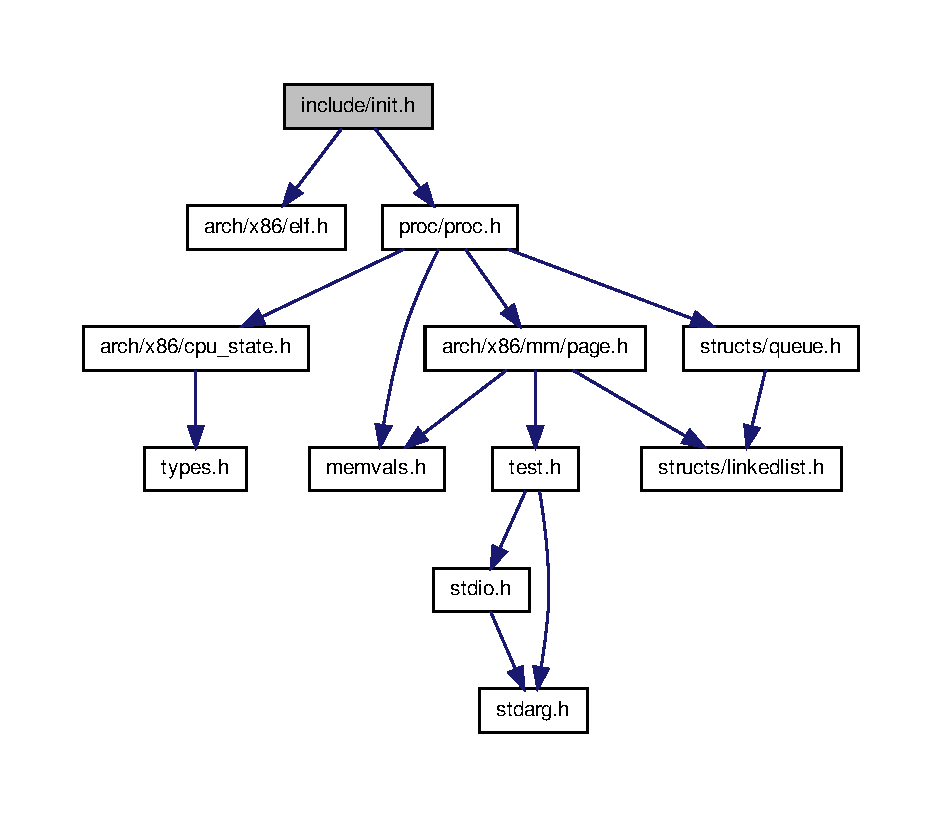
\includegraphics[width=350pt]{init_8h__incl}
\end{center}
\end{figure}
\-This graph shows which files directly or indirectly include this file\-:\nopagebreak
\begin{figure}[H]
\begin{center}
\leavevmode
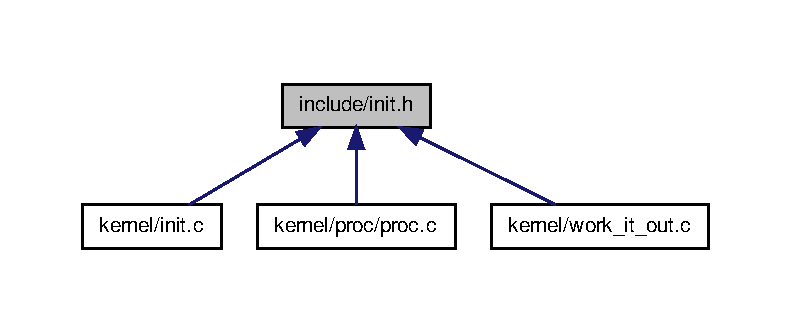
\includegraphics[width=350pt]{init_8h__dep__incl}
\end{center}
\end{figure}
\subsection*{\-Defines}
\begin{DoxyCompactItemize}
\item 
\#define \hyperlink{init_8h_a3bb20c9a153cc24ad25ef57d9e1e2db6}{\-E\-L\-F\-H\-D\-R}~((struct \hyperlink{structelfhdr}{elfhdr} $\ast$) 0x\-A0000000)
\item 
\#define \hyperlink{init_8h_af7ab12df78ebefa2212fca77338f56cd}{\-S\-E\-C\-T\-O\-R}~512
\end{DoxyCompactItemize}
\subsection*{\-Functions}
\begin{DoxyCompactItemize}
\item 
void \hyperlink{init_8h_a8550587b9b0a5d791fb2a9917415f6c5}{\-Init\-\_\-userspace} (\hyperlink{proc_8h_abcae78bfd085fccd601f7cc568946453}{proc\-\_\-t} $\ast$)
\end{DoxyCompactItemize}


\subsection{\-Define \-Documentation}
\hypertarget{init_8h_a3bb20c9a153cc24ad25ef57d9e1e2db6}{\index{init.\-h@{init.\-h}!\-E\-L\-F\-H\-D\-R@{\-E\-L\-F\-H\-D\-R}}
\index{\-E\-L\-F\-H\-D\-R@{\-E\-L\-F\-H\-D\-R}!init.h@{init.\-h}}
\subsubsection[{\-E\-L\-F\-H\-D\-R}]{\setlength{\rightskip}{0pt plus 5cm}\#define {\bf \-E\-L\-F\-H\-D\-R}~((struct {\bf elfhdr} $\ast$) 0x\-A0000000)}}\label{init_8h_a3bb20c9a153cc24ad25ef57d9e1e2db6}


\-Definition at line 5 of file init.\-h.

\hypertarget{init_8h_af7ab12df78ebefa2212fca77338f56cd}{\index{init.\-h@{init.\-h}!\-S\-E\-C\-T\-O\-R@{\-S\-E\-C\-T\-O\-R}}
\index{\-S\-E\-C\-T\-O\-R@{\-S\-E\-C\-T\-O\-R}!init.h@{init.\-h}}
\subsubsection[{\-S\-E\-C\-T\-O\-R}]{\setlength{\rightskip}{0pt plus 5cm}\#define {\bf \-S\-E\-C\-T\-O\-R}~512}}\label{init_8h_af7ab12df78ebefa2212fca77338f56cd}


\-Definition at line 6 of file init.\-h.



\subsection{\-Function \-Documentation}
\hypertarget{init_8h_a8550587b9b0a5d791fb2a9917415f6c5}{\index{init.\-h@{init.\-h}!\-Init\-\_\-userspace@{\-Init\-\_\-userspace}}
\index{\-Init\-\_\-userspace@{\-Init\-\_\-userspace}!init.h@{init.\-h}}
\subsubsection[{\-Init\-\_\-userspace}]{\setlength{\rightskip}{0pt plus 5cm}void {\bf \-Init\-\_\-userspace} (
\begin{DoxyParamCaption}
\item[{{\bf proc\-\_\-t} $\ast$}]{}
\end{DoxyParamCaption}
)}}\label{init_8h_a8550587b9b0a5d791fb2a9917415f6c5}


\-Definition at line 16 of file init.\-c.


\hypertarget{kbc_8h}{\section{include/kbc.h \-File \-Reference}
\label{kbc_8h}\index{include/kbc.\-h@{include/kbc.\-h}}
}
{\ttfamily \#include $<$types.\-h$>$}\*
\-Include dependency graph for kbc.\-h\-:\nopagebreak
\begin{figure}[H]
\begin{center}
\leavevmode
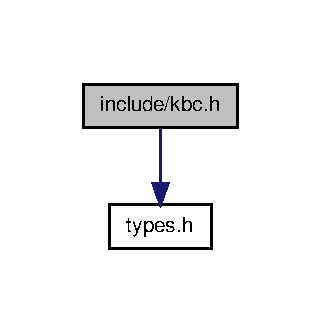
\includegraphics[width=154pt]{kbc_8h__incl}
\end{center}
\end{figure}
\-This graph shows which files directly or indirectly include this file\-:\nopagebreak
\begin{figure}[H]
\begin{center}
\leavevmode
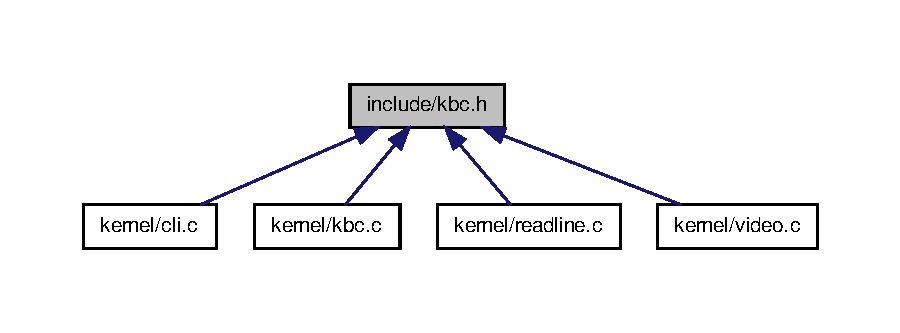
\includegraphics[width=350pt]{kbc_8h__dep__incl}
\end{center}
\end{figure}
\subsection*{\-Defines}
\begin{DoxyCompactItemize}
\item 
\#define \hyperlink{kbc_8h_afd321581da9c009e77ca77612d026ec2}{\-K\-B\-C\-\_\-\-S\-T\-A\-T\-U\-S\-P\-O\-R\-T}~0x64
\item 
\#define \hyperlink{kbc_8h_a83c26cee464c0bd0739a99ef60c368f7}{\-K\-B\-C\-\_\-\-D\-A\-T\-A\-P\-O\-R\-T}~0x60
\item 
\#define \hyperlink{kbc_8h_ad10c1d496e696488559cde113317fec5}{\-K\-B\-C\-\_\-\-D\-A\-T\-A\-I\-N}~0x01	/$\ast$$\ast$ New Data in buffer $\ast$$\ast$/
\item 
\#define \hyperlink{kbc_8h_af6319137ba2e75ef1353729f014bef1b}{\-K\-B\-C\-\_\-\-F\-U\-L\-L\-B\-U\-F}~0x02	/$\ast$$\ast$ Buffer is full $\ast$$\ast$/
\item 
\#define \hyperlink{kbc_8h_ac93554216ffddf26f4cd30a5914bd9fa}{\-K\-B\-C\-\_\-\-R\-E\-B\-O\-O\-T}~0x04	/$\ast$$\ast$ soft reboot $\ast$$\ast$/
\item 
\#define \hyperlink{kbc_8h_a0d562a66341b00a3e2491bbeb5a20d5d}{\-K\-B\-C\-\_\-\-C\-O\-M\-M\-A\-N\-D}~0x08	/$\ast$$\ast$ data in output register is a command $\ast$$\ast$/
\item 
\#define \hyperlink{kbc_8h_ae67c9300c0b90b81e55ecf8313c20952}{\-K\-B\-C\-\_\-\-S\-E\-C\-L\-O\-C\-K}~0x10	/$\ast$$\ast$ Security lock engaged $\ast$$\ast$/
\item 
\#define \hyperlink{kbc_8h_ac10ad9ebfd3e267d59e6fa55cc22b1a7}{\-K\-B\-C\-\_\-\-T\-T\-I\-M\-E\-O\-U\-T}~0x20	/$\ast$$\ast$ transmission timeout error $\ast$$\ast$/
\item 
\#define \hyperlink{kbc_8h_a33677a3374da89e2aea99e70043c0669}{\-K\-B\-C\-\_\-\-R\-T\-I\-M\-E\-O\-U\-T}~0x40	/$\ast$$\ast$ recieve timeout error $\ast$$\ast$/
\item 
\#define \hyperlink{kbc_8h_a82a39176e42fe8f48025521b9674cdc6}{\-K\-B\-C\-\_\-\-P\-A\-R\-I\-T\-Y}~0x80	/$\ast$$\ast$ Parity error $\ast$$\ast$/
\item 
\#define \hyperlink{kbc_8h_a3d7de39b369f644585feb4cabd643f9f}{\-K\-B\-C\-\_\-\-R\-E\-A\-D\-R\-A\-M}~0x20	/$\ast$$\ast$ Read byte 0 from the internal R\-A\-M $\ast$$\ast$/
\item 
\#define \hyperlink{kbc_8h_a1072189fb81979edebf1c1f6eb6df535}{\-K\-B\-C\-\_\-\-R\-E\-A\-D\-L\-O\-W}~0x21	/$\ast$$\ast$ Read byte specified in low 5 bits of the command in 804x's internal R\-A\-M $\ast$$\ast$/
\item 
\#define \hyperlink{kbc_8h_aee9938edf70d141725e4c3a031007baa}{\-K\-B\-C\-\_\-\-W\-R\-I\-T\-E\-R\-A\-M}~0x60	/$\ast$$\ast$ write the data to the address specified in the 5 lower bits of command $\ast$$\ast$/
\item 
\#define \hyperlink{kbc_8h_abd5d90340251eb8295f57d966234df95}{\-K\-B\-C\-\_\-\-D\-I\-S\-M\-O\-U\-S\-E}~0x\-A7	/$\ast$$\ast$ disable mouse/auxillary port $\ast$$\ast$/
\item 
\#define \hyperlink{kbc_8h_ab255fc48bcc371829b66cc2c84a49553}{\-K\-B\-C\-\_\-\-E\-N\-M\-O\-U\-S\-E}~0x\-A8	/$\ast$$\ast$ enable mouse/auxillary port $\ast$$\ast$/
\item 
\#define \hyperlink{kbc_8h_ab6421575437acd520cbcc6829d998bdd}{\-K\-B\-C\-\_\-\-T\-S\-T\-M\-O\-U\-S\-E}~0x\-A9	/$\ast$$\ast$ test mouse/auxillary port $\ast$$\ast$/
\item 
\#define \hyperlink{kbc_8h_a3b6e93597b428f09d15500b9924a2dbe}{\-K\-B\-C\-\_\-\-S\-E\-L\-F\-T\-E\-S\-T}~0x\-A\-A	/$\ast$$\ast$ initiate the self-\/test $\ast$$\ast$/
\item 
\#define \hyperlink{kbc_8h_a7208ef5cf529564551b6ad7571126057}{\-K\-B\-C\-\_\-\-I\-N\-T\-R\-T\-E\-S\-T}
\item 
\#define \hyperlink{kbc_8h_a66904faee9c4ce70afd7e6e7db02b566}{\-K\-B\-C\-\_\-\-D\-I\-G\-D\-U\-M\-P}~0x\-A\-C 	/$\ast$$\ast$ dump the content of 804x's R\-A\-M, output port, input port, status word $\ast$$\ast$/
\item 
\#define \hyperlink{kbc_8h_a5867d36b2e13ae3f101e84fa0f5eb12f}{\-K\-B\-C\-\_\-\-D\-I\-S\-K\-B\-D}~0x\-A\-D	/$\ast$$\ast$ disable keyboard $\ast$$\ast$/
\item 
\#define \hyperlink{kbc_8h_a74df832f0d7b6d8a51e5884f75935d25}{\-K\-B\-C\-\_\-\-E\-N\-B\-K\-B\-D}~0x\-A\-E	/$\ast$$\ast$ enable keyboard $\ast$$\ast$/
\item 
\#define \hyperlink{kbc_8h_a108efc17e6b60d69db8579b0cf23f79a}{\-K\-B\-C\-\_\-\-R\-E\-A\-D\-V\-E\-R}~0x\-A\-F	/$\ast$$\ast$ Read keyboard version $\ast$$\ast$/
\item 
\#define \hyperlink{kbc_8h_a6e071b5150a91ec4dabda75dad679149}{\-K\-B\-C\-\_\-\-I\-N\-P\-R\-E\-A\-D}~0x\-C0	/$\ast$$\ast$ Read input port $\ast$$\ast$/
\item 
\#define \hyperlink{kbc_8h_adaf92e130cdbd5611a360198233201dd}{\-K\-B\-C\-\_\-\-O\-U\-T\-R\-E\-A\-D}~0x\-D0	/$\ast$$\ast$ Read Output port $\ast$$\ast$/
\item 
\#define \hyperlink{kbc_8h_a1879110de3cf58035d08b4572ae449f9}{\-K\-B\-C\-\_\-\-O\-U\-T\-W\-R\-T\-E}~0x\-D1	/$\ast$$\ast$ write output port ,next byte will be written to 804x $\ast$$\ast$/
\item 
\#define \hyperlink{kbc_8h_ad10691bb2a88fe0599b3dcc14ef904de}{\-K\-B\-C\-\_\-\-O\-U\-T\-K\-B\-D}~0x\-D2	/$\ast$$\ast$ Echo keyboard output buffer $\ast$$\ast$/
\item 
\#define \hyperlink{kbc_8h_a48e4b03f7be349754c77099d35f21d20}{\-K\-B\-C\-\_\-\-O\-U\-T\-A\-U\-X}~0x\-D3	/$\ast$$\ast$ Echo pointing device output buffer $\ast$$\ast$/
\item 
\#define \hyperlink{kbc_8h_ab0fc656184808bac874fbaff1c4a7cc8}{\-K\-B\-C\-\_\-\-A\-U\-X\-W\-R\-I\-T\-E}~0x\-D4	/$\ast$$\ast$ Write to pointing device output buffer $\ast$$\ast$/
\item 
\#define \hyperlink{kbc_8h_ab4a5907532b9ecdec56d528a93dac558}{\-K\-B\-C\-\_\-\-D\-I\-S\-A20}~0x\-D\-D	/$\ast$$\ast$ Disable the A20 gate $\ast$$\ast$/
\item 
\#define \hyperlink{kbc_8h_aa5033fcf2ff94d8efffd64fccf98ffa5}{\-K\-B\-C\-\_\-\-E\-N\-B\-A20}~0x\-D\-F	/$\ast$$\ast$ Enable the A20 gate $\ast$$\ast$/
\item 
\#define \hyperlink{kbc_8h_a6a2a046aa363ac58ce6ddb0a4ddc3b0b}{\-K\-B\-C\-\_\-\-P\-U\-L\-S\-E0}~0x\-F\-E	/$\ast$$\ast$ Pulse output bit 0 $\ast$$\ast$/
\item 
\#define \hyperlink{kbc_8h_ae96097ff8247c0f4b6c9e3bc5afd6ebc}{\-K\-B\-C\-\_\-\-P\-U\-L\-S\-E1}~0x\-F\-D	/$\ast$$\ast$ $\sim$$\sim$$\sim$$\sim$$\sim$$\sim$$\sim$$\sim$$\sim$$\sim$$\sim$$\sim$$\sim$$\sim$$\sim$$\sim$ 1 $\ast$$\ast$/
\item 
\#define \hyperlink{kbc_8h_afa4d6fe554e5b3f8181e38e3c4366f11}{\-K\-B\-C\-\_\-\-P\-U\-L\-S\-E2}~0x\-F\-B	/$\ast$$\ast$ $\sim$$\sim$$\sim$$\sim$$\sim$$\sim$$\sim$$\sim$$\sim$$\sim$$\sim$$\sim$$\sim$$\sim$$\sim$$\sim$ 2 $\ast$$\ast$/
\item 
\#define \hyperlink{kbc_8h_af5b1025d8b69021f483d35ef69c3f1de}{\-K\-B\-C\-\_\-\-P\-U\-L\-S\-E3}~0x\-F7	/$\ast$$\ast$ $\sim$$\sim$$\sim$$\sim$$\sim$$\sim$$\sim$$\sim$$\sim$$\sim$$\sim$$\sim$$\sim$$\sim$$\sim$$\sim$ 3 $\ast$$\ast$/
\item 
\#define \hyperlink{kbc_8h_a9380d340e2f61e3cc7ab35345f9d47d8}{\-K\-B\-C\-\_\-\-R\-E\-S\-E\-T}~0x\-F\-F	/$\ast$$\ast$ R\-E\-S\-E\-T the mouse and the keyboard $\ast$$\ast$/
\item 
\#define \hyperlink{kbc_8h_a5e88c9afa8efac0728e8483135b7ceb5}{\-K\-B\-C\-\_\-\-R\-E\-S\-E\-N\-D}~0x\-F\-E	/$\ast$$\ast$ Resend the last byte $\ast$$\ast$/
\item 
\#define \hyperlink{kbc_8h_a27dc41c3dca8a932afe0a30c5e239224}{\-K\-B\-C\-\_\-\-D\-E\-F\-A\-U\-L\-T}~0x\-F6	/$\ast$$\ast$ Set the keyboard to default parameters $\ast$$\ast$/
\item 
\#define \hyperlink{kbc_8h_aeaea276e8eeadf22fe2508dfe15d0fc8}{\-K\-B\-C\-\_\-\-D\-I\-S\-A\-B\-L\-E}~0x\-F5	/$\ast$$\ast$ disables key scanning, yet set the default parameters $\ast$$\ast$/
\item 
\#define \hyperlink{kbc_8h_a291939465a5c59ca219f53201eb4da75}{\-K\-B\-C\-\_\-\-E\-N\-A\-B\-L\-E}~0x\-F4	/$\ast$$\ast$ Enable key scanning $\ast$$\ast$/
\item 
\#define \hyperlink{kbc_8h_aad7b69b6846a7ec0718fbed27088ae0e}{\-K\-B\-C\-\_\-\-T\-Y\-P\-E\-M\-A\-T\-I\-C}~0x\-F3	/$\ast$$\ast$ Set typematic rate/delay $\ast$$\ast$/
\item 
\#define \hyperlink{kbc_8h_a893a8f21fee8b56d5bad81cd7fe7a012}{\-K\-B\-C\-\_\-\-R\-E\-A\-D\-I\-D}~0x\-F2	/$\ast$$\ast$ Read Keyboard I\-D $\ast$$\ast$/
\item 
\#define \hyperlink{kbc_8h_a04a4fc50a5d92c2f70a62e3f26a05e55}{\-K\-B\-C\-\_\-\-S\-E\-T\-S\-C\-A\-N}~0x\-F0	/$\ast$$\ast$ Set/\-Get scancodes set $\ast$$\ast$/
\item 
\#define \hyperlink{kbc_8h_a1169d58bb478567093f07168a34395c7}{\-K\-B\-C\-\_\-\-E\-C\-H\-O\-D\-I\-G}~0x\-E\-E	/$\ast$$\ast$ request a diganostic echo from the keyboard $\ast$$\ast$/
\item 
\#define \hyperlink{kbc_8h_a741fc4238c68fc68bd3a1f6ee565fc63}{\-K\-B\-C\-\_\-\-I\-N\-D\-I\-C\-A\-T\-O\-R}~0x\-E\-D	/$\ast$$\ast$ Set mode indicators $\ast$$\ast$/
\item 
\#define \hyperlink{kbc_8h_af6806366178266b3eaf1fb16f991cbee}{\-K\-E\-Y\-\_\-\-H\-O\-M\-E}~0x\-E0
\item 
\#define \hyperlink{kbc_8h_a912861b945e779c29f718cdcd62be10c}{\-K\-E\-Y\-\_\-\-E\-N\-D}~0x\-E1
\item 
\#define \hyperlink{kbc_8h_afa086fc916a81e7fd348ec00cf786916}{\-K\-E\-Y\-\_\-\-U\-P}~0x\-E2
\item 
\#define \hyperlink{kbc_8h_a69aff5c97fd814c5f29fca79bdcda9be}{\-K\-E\-Y\-\_\-\-D\-N}~0x\-E3
\item 
\#define \hyperlink{kbc_8h_afe0182b9752acbeff23e5b01e63ffe9c}{\-K\-E\-Y\-\_\-\-L\-F}~0x\-E4
\item 
\#define \hyperlink{kbc_8h_ab787b56ca072749c919b02381f66d271}{\-K\-E\-Y\-\_\-\-R\-T}~0x\-E5
\item 
\#define \hyperlink{kbc_8h_ac35c65d4a20c05b2cc7e1f3e40e13e79}{\-K\-E\-Y\-\_\-\-P\-G\-U\-P}~0x\-E6
\item 
\#define \hyperlink{kbc_8h_a84a56bcd66075dce29dd77873006f33c}{\-K\-E\-Y\-\_\-\-P\-G\-D\-N}~0x\-E7
\item 
\#define \hyperlink{kbc_8h_a4ea8f40f4220377b764d1b3b14807f2b}{\-K\-E\-Y\-\_\-\-I\-N\-S}~0x\-E8
\item 
\#define \hyperlink{kbc_8h_ad06e66a899b065c65c2363233d8ebce2}{\-K\-E\-Y\-\_\-\-D\-E\-L}~0x\-E9
\end{DoxyCompactItemize}
\subsection*{\-Functions}
\begin{DoxyCompactItemize}
\item 
int \hyperlink{kbc_8h_aa8584463ac58034ccbf9cd2ffc8e187d}{kbc\-\_\-data} (void)
\item 
void \hyperlink{kbc_8h_abf3ce1c314db9a6a15b99e5313eb2edb}{kbc\-\_\-interrupt} (void)
\end{DoxyCompactItemize}


\subsection{\-Define \-Documentation}
\hypertarget{kbc_8h_ab0fc656184808bac874fbaff1c4a7cc8}{\index{kbc.\-h@{kbc.\-h}!\-K\-B\-C\-\_\-\-A\-U\-X\-W\-R\-I\-T\-E@{\-K\-B\-C\-\_\-\-A\-U\-X\-W\-R\-I\-T\-E}}
\index{\-K\-B\-C\-\_\-\-A\-U\-X\-W\-R\-I\-T\-E@{\-K\-B\-C\-\_\-\-A\-U\-X\-W\-R\-I\-T\-E}!kbc.h@{kbc.\-h}}
\subsubsection[{\-K\-B\-C\-\_\-\-A\-U\-X\-W\-R\-I\-T\-E}]{\setlength{\rightskip}{0pt plus 5cm}\#define {\bf \-K\-B\-C\-\_\-\-A\-U\-X\-W\-R\-I\-T\-E}~0x\-D4	/$\ast$$\ast$ Write to pointing device output buffer $\ast$$\ast$/}}\label{kbc_8h_ab0fc656184808bac874fbaff1c4a7cc8}


\-Definition at line 40 of file kbc.\-h.

\hypertarget{kbc_8h_a0d562a66341b00a3e2491bbeb5a20d5d}{\index{kbc.\-h@{kbc.\-h}!\-K\-B\-C\-\_\-\-C\-O\-M\-M\-A\-N\-D@{\-K\-B\-C\-\_\-\-C\-O\-M\-M\-A\-N\-D}}
\index{\-K\-B\-C\-\_\-\-C\-O\-M\-M\-A\-N\-D@{\-K\-B\-C\-\_\-\-C\-O\-M\-M\-A\-N\-D}!kbc.h@{kbc.\-h}}
\subsubsection[{\-K\-B\-C\-\_\-\-C\-O\-M\-M\-A\-N\-D}]{\setlength{\rightskip}{0pt plus 5cm}\#define {\bf \-K\-B\-C\-\_\-\-C\-O\-M\-M\-A\-N\-D}~0x08	/$\ast$$\ast$ data in output register is a command $\ast$$\ast$/}}\label{kbc_8h_a0d562a66341b00a3e2491bbeb5a20d5d}


\-Definition at line 16 of file kbc.\-h.

\hypertarget{kbc_8h_ad10c1d496e696488559cde113317fec5}{\index{kbc.\-h@{kbc.\-h}!\-K\-B\-C\-\_\-\-D\-A\-T\-A\-I\-N@{\-K\-B\-C\-\_\-\-D\-A\-T\-A\-I\-N}}
\index{\-K\-B\-C\-\_\-\-D\-A\-T\-A\-I\-N@{\-K\-B\-C\-\_\-\-D\-A\-T\-A\-I\-N}!kbc.h@{kbc.\-h}}
\subsubsection[{\-K\-B\-C\-\_\-\-D\-A\-T\-A\-I\-N}]{\setlength{\rightskip}{0pt plus 5cm}\#define {\bf \-K\-B\-C\-\_\-\-D\-A\-T\-A\-I\-N}~0x01	/$\ast$$\ast$ New Data in buffer $\ast$$\ast$/}}\label{kbc_8h_ad10c1d496e696488559cde113317fec5}


\-Definition at line 13 of file kbc.\-h.

\hypertarget{kbc_8h_a83c26cee464c0bd0739a99ef60c368f7}{\index{kbc.\-h@{kbc.\-h}!\-K\-B\-C\-\_\-\-D\-A\-T\-A\-P\-O\-R\-T@{\-K\-B\-C\-\_\-\-D\-A\-T\-A\-P\-O\-R\-T}}
\index{\-K\-B\-C\-\_\-\-D\-A\-T\-A\-P\-O\-R\-T@{\-K\-B\-C\-\_\-\-D\-A\-T\-A\-P\-O\-R\-T}!kbc.h@{kbc.\-h}}
\subsubsection[{\-K\-B\-C\-\_\-\-D\-A\-T\-A\-P\-O\-R\-T}]{\setlength{\rightskip}{0pt plus 5cm}\#define {\bf \-K\-B\-C\-\_\-\-D\-A\-T\-A\-P\-O\-R\-T}~0x60}}\label{kbc_8h_a83c26cee464c0bd0739a99ef60c368f7}


\-Definition at line 11 of file kbc.\-h.

\hypertarget{kbc_8h_a27dc41c3dca8a932afe0a30c5e239224}{\index{kbc.\-h@{kbc.\-h}!\-K\-B\-C\-\_\-\-D\-E\-F\-A\-U\-L\-T@{\-K\-B\-C\-\_\-\-D\-E\-F\-A\-U\-L\-T}}
\index{\-K\-B\-C\-\_\-\-D\-E\-F\-A\-U\-L\-T@{\-K\-B\-C\-\_\-\-D\-E\-F\-A\-U\-L\-T}!kbc.h@{kbc.\-h}}
\subsubsection[{\-K\-B\-C\-\_\-\-D\-E\-F\-A\-U\-L\-T}]{\setlength{\rightskip}{0pt plus 5cm}\#define {\bf \-K\-B\-C\-\_\-\-D\-E\-F\-A\-U\-L\-T}~0x\-F6	/$\ast$$\ast$ Set the keyboard to default parameters $\ast$$\ast$/}}\label{kbc_8h_a27dc41c3dca8a932afe0a30c5e239224}


\-Definition at line 52 of file kbc.\-h.

\hypertarget{kbc_8h_a66904faee9c4ce70afd7e6e7db02b566}{\index{kbc.\-h@{kbc.\-h}!\-K\-B\-C\-\_\-\-D\-I\-G\-D\-U\-M\-P@{\-K\-B\-C\-\_\-\-D\-I\-G\-D\-U\-M\-P}}
\index{\-K\-B\-C\-\_\-\-D\-I\-G\-D\-U\-M\-P@{\-K\-B\-C\-\_\-\-D\-I\-G\-D\-U\-M\-P}!kbc.h@{kbc.\-h}}
\subsubsection[{\-K\-B\-C\-\_\-\-D\-I\-G\-D\-U\-M\-P}]{\setlength{\rightskip}{0pt plus 5cm}\#define {\bf \-K\-B\-C\-\_\-\-D\-I\-G\-D\-U\-M\-P}~0x\-A\-C 	/$\ast$$\ast$ dump the content of 804x's R\-A\-M, output port, input port, status word $\ast$$\ast$/}}\label{kbc_8h_a66904faee9c4ce70afd7e6e7db02b566}


\-Definition at line 31 of file kbc.\-h.

\hypertarget{kbc_8h_ab4a5907532b9ecdec56d528a93dac558}{\index{kbc.\-h@{kbc.\-h}!\-K\-B\-C\-\_\-\-D\-I\-S\-A20@{\-K\-B\-C\-\_\-\-D\-I\-S\-A20}}
\index{\-K\-B\-C\-\_\-\-D\-I\-S\-A20@{\-K\-B\-C\-\_\-\-D\-I\-S\-A20}!kbc.h@{kbc.\-h}}
\subsubsection[{\-K\-B\-C\-\_\-\-D\-I\-S\-A20}]{\setlength{\rightskip}{0pt plus 5cm}\#define {\bf \-K\-B\-C\-\_\-\-D\-I\-S\-A20}~0x\-D\-D	/$\ast$$\ast$ Disable the A20 gate $\ast$$\ast$/}}\label{kbc_8h_ab4a5907532b9ecdec56d528a93dac558}


\-Definition at line 41 of file kbc.\-h.

\hypertarget{kbc_8h_aeaea276e8eeadf22fe2508dfe15d0fc8}{\index{kbc.\-h@{kbc.\-h}!\-K\-B\-C\-\_\-\-D\-I\-S\-A\-B\-L\-E@{\-K\-B\-C\-\_\-\-D\-I\-S\-A\-B\-L\-E}}
\index{\-K\-B\-C\-\_\-\-D\-I\-S\-A\-B\-L\-E@{\-K\-B\-C\-\_\-\-D\-I\-S\-A\-B\-L\-E}!kbc.h@{kbc.\-h}}
\subsubsection[{\-K\-B\-C\-\_\-\-D\-I\-S\-A\-B\-L\-E}]{\setlength{\rightskip}{0pt plus 5cm}\#define {\bf \-K\-B\-C\-\_\-\-D\-I\-S\-A\-B\-L\-E}~0x\-F5	/$\ast$$\ast$ disables key scanning, yet set the default parameters $\ast$$\ast$/}}\label{kbc_8h_aeaea276e8eeadf22fe2508dfe15d0fc8}


\-Definition at line 53 of file kbc.\-h.

\hypertarget{kbc_8h_a5867d36b2e13ae3f101e84fa0f5eb12f}{\index{kbc.\-h@{kbc.\-h}!\-K\-B\-C\-\_\-\-D\-I\-S\-K\-B\-D@{\-K\-B\-C\-\_\-\-D\-I\-S\-K\-B\-D}}
\index{\-K\-B\-C\-\_\-\-D\-I\-S\-K\-B\-D@{\-K\-B\-C\-\_\-\-D\-I\-S\-K\-B\-D}!kbc.h@{kbc.\-h}}
\subsubsection[{\-K\-B\-C\-\_\-\-D\-I\-S\-K\-B\-D}]{\setlength{\rightskip}{0pt plus 5cm}\#define {\bf \-K\-B\-C\-\_\-\-D\-I\-S\-K\-B\-D}~0x\-A\-D	/$\ast$$\ast$ disable keyboard $\ast$$\ast$/}}\label{kbc_8h_a5867d36b2e13ae3f101e84fa0f5eb12f}


\-Definition at line 32 of file kbc.\-h.

\hypertarget{kbc_8h_abd5d90340251eb8295f57d966234df95}{\index{kbc.\-h@{kbc.\-h}!\-K\-B\-C\-\_\-\-D\-I\-S\-M\-O\-U\-S\-E@{\-K\-B\-C\-\_\-\-D\-I\-S\-M\-O\-U\-S\-E}}
\index{\-K\-B\-C\-\_\-\-D\-I\-S\-M\-O\-U\-S\-E@{\-K\-B\-C\-\_\-\-D\-I\-S\-M\-O\-U\-S\-E}!kbc.h@{kbc.\-h}}
\subsubsection[{\-K\-B\-C\-\_\-\-D\-I\-S\-M\-O\-U\-S\-E}]{\setlength{\rightskip}{0pt plus 5cm}\#define {\bf \-K\-B\-C\-\_\-\-D\-I\-S\-M\-O\-U\-S\-E}~0x\-A7	/$\ast$$\ast$ disable mouse/auxillary port $\ast$$\ast$/}}\label{kbc_8h_abd5d90340251eb8295f57d966234df95}


\-Definition at line 26 of file kbc.\-h.

\hypertarget{kbc_8h_a1169d58bb478567093f07168a34395c7}{\index{kbc.\-h@{kbc.\-h}!\-K\-B\-C\-\_\-\-E\-C\-H\-O\-D\-I\-G@{\-K\-B\-C\-\_\-\-E\-C\-H\-O\-D\-I\-G}}
\index{\-K\-B\-C\-\_\-\-E\-C\-H\-O\-D\-I\-G@{\-K\-B\-C\-\_\-\-E\-C\-H\-O\-D\-I\-G}!kbc.h@{kbc.\-h}}
\subsubsection[{\-K\-B\-C\-\_\-\-E\-C\-H\-O\-D\-I\-G}]{\setlength{\rightskip}{0pt plus 5cm}\#define {\bf \-K\-B\-C\-\_\-\-E\-C\-H\-O\-D\-I\-G}~0x\-E\-E	/$\ast$$\ast$ request a diganostic echo from the keyboard $\ast$$\ast$/}}\label{kbc_8h_a1169d58bb478567093f07168a34395c7}


\-Definition at line 58 of file kbc.\-h.

\hypertarget{kbc_8h_a291939465a5c59ca219f53201eb4da75}{\index{kbc.\-h@{kbc.\-h}!\-K\-B\-C\-\_\-\-E\-N\-A\-B\-L\-E@{\-K\-B\-C\-\_\-\-E\-N\-A\-B\-L\-E}}
\index{\-K\-B\-C\-\_\-\-E\-N\-A\-B\-L\-E@{\-K\-B\-C\-\_\-\-E\-N\-A\-B\-L\-E}!kbc.h@{kbc.\-h}}
\subsubsection[{\-K\-B\-C\-\_\-\-E\-N\-A\-B\-L\-E}]{\setlength{\rightskip}{0pt plus 5cm}\#define {\bf \-K\-B\-C\-\_\-\-E\-N\-A\-B\-L\-E}~0x\-F4	/$\ast$$\ast$ Enable key scanning $\ast$$\ast$/}}\label{kbc_8h_a291939465a5c59ca219f53201eb4da75}


\-Definition at line 54 of file kbc.\-h.

\hypertarget{kbc_8h_aa5033fcf2ff94d8efffd64fccf98ffa5}{\index{kbc.\-h@{kbc.\-h}!\-K\-B\-C\-\_\-\-E\-N\-B\-A20@{\-K\-B\-C\-\_\-\-E\-N\-B\-A20}}
\index{\-K\-B\-C\-\_\-\-E\-N\-B\-A20@{\-K\-B\-C\-\_\-\-E\-N\-B\-A20}!kbc.h@{kbc.\-h}}
\subsubsection[{\-K\-B\-C\-\_\-\-E\-N\-B\-A20}]{\setlength{\rightskip}{0pt plus 5cm}\#define {\bf \-K\-B\-C\-\_\-\-E\-N\-B\-A20}~0x\-D\-F	/$\ast$$\ast$ Enable the A20 gate $\ast$$\ast$/}}\label{kbc_8h_aa5033fcf2ff94d8efffd64fccf98ffa5}


\-Definition at line 42 of file kbc.\-h.

\hypertarget{kbc_8h_a74df832f0d7b6d8a51e5884f75935d25}{\index{kbc.\-h@{kbc.\-h}!\-K\-B\-C\-\_\-\-E\-N\-B\-K\-B\-D@{\-K\-B\-C\-\_\-\-E\-N\-B\-K\-B\-D}}
\index{\-K\-B\-C\-\_\-\-E\-N\-B\-K\-B\-D@{\-K\-B\-C\-\_\-\-E\-N\-B\-K\-B\-D}!kbc.h@{kbc.\-h}}
\subsubsection[{\-K\-B\-C\-\_\-\-E\-N\-B\-K\-B\-D}]{\setlength{\rightskip}{0pt plus 5cm}\#define {\bf \-K\-B\-C\-\_\-\-E\-N\-B\-K\-B\-D}~0x\-A\-E	/$\ast$$\ast$ enable keyboard $\ast$$\ast$/}}\label{kbc_8h_a74df832f0d7b6d8a51e5884f75935d25}


\-Definition at line 33 of file kbc.\-h.

\hypertarget{kbc_8h_ab255fc48bcc371829b66cc2c84a49553}{\index{kbc.\-h@{kbc.\-h}!\-K\-B\-C\-\_\-\-E\-N\-M\-O\-U\-S\-E@{\-K\-B\-C\-\_\-\-E\-N\-M\-O\-U\-S\-E}}
\index{\-K\-B\-C\-\_\-\-E\-N\-M\-O\-U\-S\-E@{\-K\-B\-C\-\_\-\-E\-N\-M\-O\-U\-S\-E}!kbc.h@{kbc.\-h}}
\subsubsection[{\-K\-B\-C\-\_\-\-E\-N\-M\-O\-U\-S\-E}]{\setlength{\rightskip}{0pt plus 5cm}\#define {\bf \-K\-B\-C\-\_\-\-E\-N\-M\-O\-U\-S\-E}~0x\-A8	/$\ast$$\ast$ enable mouse/auxillary port $\ast$$\ast$/}}\label{kbc_8h_ab255fc48bcc371829b66cc2c84a49553}


\-Definition at line 27 of file kbc.\-h.

\hypertarget{kbc_8h_af6319137ba2e75ef1353729f014bef1b}{\index{kbc.\-h@{kbc.\-h}!\-K\-B\-C\-\_\-\-F\-U\-L\-L\-B\-U\-F@{\-K\-B\-C\-\_\-\-F\-U\-L\-L\-B\-U\-F}}
\index{\-K\-B\-C\-\_\-\-F\-U\-L\-L\-B\-U\-F@{\-K\-B\-C\-\_\-\-F\-U\-L\-L\-B\-U\-F}!kbc.h@{kbc.\-h}}
\subsubsection[{\-K\-B\-C\-\_\-\-F\-U\-L\-L\-B\-U\-F}]{\setlength{\rightskip}{0pt plus 5cm}\#define {\bf \-K\-B\-C\-\_\-\-F\-U\-L\-L\-B\-U\-F}~0x02	/$\ast$$\ast$ Buffer is full $\ast$$\ast$/}}\label{kbc_8h_af6319137ba2e75ef1353729f014bef1b}


\-Definition at line 14 of file kbc.\-h.

\hypertarget{kbc_8h_a741fc4238c68fc68bd3a1f6ee565fc63}{\index{kbc.\-h@{kbc.\-h}!\-K\-B\-C\-\_\-\-I\-N\-D\-I\-C\-A\-T\-O\-R@{\-K\-B\-C\-\_\-\-I\-N\-D\-I\-C\-A\-T\-O\-R}}
\index{\-K\-B\-C\-\_\-\-I\-N\-D\-I\-C\-A\-T\-O\-R@{\-K\-B\-C\-\_\-\-I\-N\-D\-I\-C\-A\-T\-O\-R}!kbc.h@{kbc.\-h}}
\subsubsection[{\-K\-B\-C\-\_\-\-I\-N\-D\-I\-C\-A\-T\-O\-R}]{\setlength{\rightskip}{0pt plus 5cm}\#define {\bf \-K\-B\-C\-\_\-\-I\-N\-D\-I\-C\-A\-T\-O\-R}~0x\-E\-D	/$\ast$$\ast$ Set mode indicators $\ast$$\ast$/}}\label{kbc_8h_a741fc4238c68fc68bd3a1f6ee565fc63}


\-Definition at line 59 of file kbc.\-h.

\hypertarget{kbc_8h_a6e071b5150a91ec4dabda75dad679149}{\index{kbc.\-h@{kbc.\-h}!\-K\-B\-C\-\_\-\-I\-N\-P\-R\-E\-A\-D@{\-K\-B\-C\-\_\-\-I\-N\-P\-R\-E\-A\-D}}
\index{\-K\-B\-C\-\_\-\-I\-N\-P\-R\-E\-A\-D@{\-K\-B\-C\-\_\-\-I\-N\-P\-R\-E\-A\-D}!kbc.h@{kbc.\-h}}
\subsubsection[{\-K\-B\-C\-\_\-\-I\-N\-P\-R\-E\-A\-D}]{\setlength{\rightskip}{0pt plus 5cm}\#define {\bf \-K\-B\-C\-\_\-\-I\-N\-P\-R\-E\-A\-D}~0x\-C0	/$\ast$$\ast$ Read input port $\ast$$\ast$/}}\label{kbc_8h_a6e071b5150a91ec4dabda75dad679149}


\-Definition at line 35 of file kbc.\-h.

\hypertarget{kbc_8h_a7208ef5cf529564551b6ad7571126057}{\index{kbc.\-h@{kbc.\-h}!\-K\-B\-C\-\_\-\-I\-N\-T\-R\-T\-E\-S\-T@{\-K\-B\-C\-\_\-\-I\-N\-T\-R\-T\-E\-S\-T}}
\index{\-K\-B\-C\-\_\-\-I\-N\-T\-R\-T\-E\-S\-T@{\-K\-B\-C\-\_\-\-I\-N\-T\-R\-T\-E\-S\-T}!kbc.h@{kbc.\-h}}
\subsubsection[{\-K\-B\-C\-\_\-\-I\-N\-T\-R\-T\-E\-S\-T}]{\setlength{\rightskip}{0pt plus 5cm}\#define {\bf \-K\-B\-C\-\_\-\-I\-N\-T\-R\-T\-E\-S\-T}}}\label{kbc_8h_a7208ef5cf529564551b6ad7571126057}
{\bfseries \-Value\-:}
\begin{DoxyCode}
0xAB    
\end{DoxyCode}


\-Definition at line 30 of file kbc.\-h.

\hypertarget{kbc_8h_a48e4b03f7be349754c77099d35f21d20}{\index{kbc.\-h@{kbc.\-h}!\-K\-B\-C\-\_\-\-O\-U\-T\-A\-U\-X@{\-K\-B\-C\-\_\-\-O\-U\-T\-A\-U\-X}}
\index{\-K\-B\-C\-\_\-\-O\-U\-T\-A\-U\-X@{\-K\-B\-C\-\_\-\-O\-U\-T\-A\-U\-X}!kbc.h@{kbc.\-h}}
\subsubsection[{\-K\-B\-C\-\_\-\-O\-U\-T\-A\-U\-X}]{\setlength{\rightskip}{0pt plus 5cm}\#define {\bf \-K\-B\-C\-\_\-\-O\-U\-T\-A\-U\-X}~0x\-D3	/$\ast$$\ast$ Echo pointing device output buffer $\ast$$\ast$/}}\label{kbc_8h_a48e4b03f7be349754c77099d35f21d20}


\-Definition at line 39 of file kbc.\-h.

\hypertarget{kbc_8h_ad10691bb2a88fe0599b3dcc14ef904de}{\index{kbc.\-h@{kbc.\-h}!\-K\-B\-C\-\_\-\-O\-U\-T\-K\-B\-D@{\-K\-B\-C\-\_\-\-O\-U\-T\-K\-B\-D}}
\index{\-K\-B\-C\-\_\-\-O\-U\-T\-K\-B\-D@{\-K\-B\-C\-\_\-\-O\-U\-T\-K\-B\-D}!kbc.h@{kbc.\-h}}
\subsubsection[{\-K\-B\-C\-\_\-\-O\-U\-T\-K\-B\-D}]{\setlength{\rightskip}{0pt plus 5cm}\#define {\bf \-K\-B\-C\-\_\-\-O\-U\-T\-K\-B\-D}~0x\-D2	/$\ast$$\ast$ Echo keyboard output buffer $\ast$$\ast$/}}\label{kbc_8h_ad10691bb2a88fe0599b3dcc14ef904de}


\-Definition at line 38 of file kbc.\-h.

\hypertarget{kbc_8h_adaf92e130cdbd5611a360198233201dd}{\index{kbc.\-h@{kbc.\-h}!\-K\-B\-C\-\_\-\-O\-U\-T\-R\-E\-A\-D@{\-K\-B\-C\-\_\-\-O\-U\-T\-R\-E\-A\-D}}
\index{\-K\-B\-C\-\_\-\-O\-U\-T\-R\-E\-A\-D@{\-K\-B\-C\-\_\-\-O\-U\-T\-R\-E\-A\-D}!kbc.h@{kbc.\-h}}
\subsubsection[{\-K\-B\-C\-\_\-\-O\-U\-T\-R\-E\-A\-D}]{\setlength{\rightskip}{0pt plus 5cm}\#define {\bf \-K\-B\-C\-\_\-\-O\-U\-T\-R\-E\-A\-D}~0x\-D0	/$\ast$$\ast$ Read Output port $\ast$$\ast$/}}\label{kbc_8h_adaf92e130cdbd5611a360198233201dd}


\-Definition at line 36 of file kbc.\-h.

\hypertarget{kbc_8h_a1879110de3cf58035d08b4572ae449f9}{\index{kbc.\-h@{kbc.\-h}!\-K\-B\-C\-\_\-\-O\-U\-T\-W\-R\-T\-E@{\-K\-B\-C\-\_\-\-O\-U\-T\-W\-R\-T\-E}}
\index{\-K\-B\-C\-\_\-\-O\-U\-T\-W\-R\-T\-E@{\-K\-B\-C\-\_\-\-O\-U\-T\-W\-R\-T\-E}!kbc.h@{kbc.\-h}}
\subsubsection[{\-K\-B\-C\-\_\-\-O\-U\-T\-W\-R\-T\-E}]{\setlength{\rightskip}{0pt plus 5cm}\#define {\bf \-K\-B\-C\-\_\-\-O\-U\-T\-W\-R\-T\-E}~0x\-D1	/$\ast$$\ast$ write output port ,next byte will be written to 804x $\ast$$\ast$/}}\label{kbc_8h_a1879110de3cf58035d08b4572ae449f9}


\-Definition at line 37 of file kbc.\-h.

\hypertarget{kbc_8h_a82a39176e42fe8f48025521b9674cdc6}{\index{kbc.\-h@{kbc.\-h}!\-K\-B\-C\-\_\-\-P\-A\-R\-I\-T\-Y@{\-K\-B\-C\-\_\-\-P\-A\-R\-I\-T\-Y}}
\index{\-K\-B\-C\-\_\-\-P\-A\-R\-I\-T\-Y@{\-K\-B\-C\-\_\-\-P\-A\-R\-I\-T\-Y}!kbc.h@{kbc.\-h}}
\subsubsection[{\-K\-B\-C\-\_\-\-P\-A\-R\-I\-T\-Y}]{\setlength{\rightskip}{0pt plus 5cm}\#define {\bf \-K\-B\-C\-\_\-\-P\-A\-R\-I\-T\-Y}~0x80	/$\ast$$\ast$ Parity error $\ast$$\ast$/}}\label{kbc_8h_a82a39176e42fe8f48025521b9674cdc6}


\-Definition at line 20 of file kbc.\-h.

\hypertarget{kbc_8h_a6a2a046aa363ac58ce6ddb0a4ddc3b0b}{\index{kbc.\-h@{kbc.\-h}!\-K\-B\-C\-\_\-\-P\-U\-L\-S\-E0@{\-K\-B\-C\-\_\-\-P\-U\-L\-S\-E0}}
\index{\-K\-B\-C\-\_\-\-P\-U\-L\-S\-E0@{\-K\-B\-C\-\_\-\-P\-U\-L\-S\-E0}!kbc.h@{kbc.\-h}}
\subsubsection[{\-K\-B\-C\-\_\-\-P\-U\-L\-S\-E0}]{\setlength{\rightskip}{0pt plus 5cm}\#define {\bf \-K\-B\-C\-\_\-\-P\-U\-L\-S\-E0}~0x\-F\-E	/$\ast$$\ast$ Pulse output bit 0 $\ast$$\ast$/}}\label{kbc_8h_a6a2a046aa363ac58ce6ddb0a4ddc3b0b}


\-Definition at line 43 of file kbc.\-h.

\hypertarget{kbc_8h_ae96097ff8247c0f4b6c9e3bc5afd6ebc}{\index{kbc.\-h@{kbc.\-h}!\-K\-B\-C\-\_\-\-P\-U\-L\-S\-E1@{\-K\-B\-C\-\_\-\-P\-U\-L\-S\-E1}}
\index{\-K\-B\-C\-\_\-\-P\-U\-L\-S\-E1@{\-K\-B\-C\-\_\-\-P\-U\-L\-S\-E1}!kbc.h@{kbc.\-h}}
\subsubsection[{\-K\-B\-C\-\_\-\-P\-U\-L\-S\-E1}]{\setlength{\rightskip}{0pt plus 5cm}\#define {\bf \-K\-B\-C\-\_\-\-P\-U\-L\-S\-E1}~0x\-F\-D	/$\ast$$\ast$ $\sim$$\sim$$\sim$$\sim$$\sim$$\sim$$\sim$$\sim$$\sim$$\sim$$\sim$$\sim$$\sim$$\sim$$\sim$$\sim$ 1 $\ast$$\ast$/}}\label{kbc_8h_ae96097ff8247c0f4b6c9e3bc5afd6ebc}


\-Definition at line 44 of file kbc.\-h.

\hypertarget{kbc_8h_afa4d6fe554e5b3f8181e38e3c4366f11}{\index{kbc.\-h@{kbc.\-h}!\-K\-B\-C\-\_\-\-P\-U\-L\-S\-E2@{\-K\-B\-C\-\_\-\-P\-U\-L\-S\-E2}}
\index{\-K\-B\-C\-\_\-\-P\-U\-L\-S\-E2@{\-K\-B\-C\-\_\-\-P\-U\-L\-S\-E2}!kbc.h@{kbc.\-h}}
\subsubsection[{\-K\-B\-C\-\_\-\-P\-U\-L\-S\-E2}]{\setlength{\rightskip}{0pt plus 5cm}\#define {\bf \-K\-B\-C\-\_\-\-P\-U\-L\-S\-E2}~0x\-F\-B	/$\ast$$\ast$ $\sim$$\sim$$\sim$$\sim$$\sim$$\sim$$\sim$$\sim$$\sim$$\sim$$\sim$$\sim$$\sim$$\sim$$\sim$$\sim$ 2 $\ast$$\ast$/}}\label{kbc_8h_afa4d6fe554e5b3f8181e38e3c4366f11}


\-Definition at line 45 of file kbc.\-h.

\hypertarget{kbc_8h_af5b1025d8b69021f483d35ef69c3f1de}{\index{kbc.\-h@{kbc.\-h}!\-K\-B\-C\-\_\-\-P\-U\-L\-S\-E3@{\-K\-B\-C\-\_\-\-P\-U\-L\-S\-E3}}
\index{\-K\-B\-C\-\_\-\-P\-U\-L\-S\-E3@{\-K\-B\-C\-\_\-\-P\-U\-L\-S\-E3}!kbc.h@{kbc.\-h}}
\subsubsection[{\-K\-B\-C\-\_\-\-P\-U\-L\-S\-E3}]{\setlength{\rightskip}{0pt plus 5cm}\#define {\bf \-K\-B\-C\-\_\-\-P\-U\-L\-S\-E3}~0x\-F7	/$\ast$$\ast$ $\sim$$\sim$$\sim$$\sim$$\sim$$\sim$$\sim$$\sim$$\sim$$\sim$$\sim$$\sim$$\sim$$\sim$$\sim$$\sim$ 3 $\ast$$\ast$/}}\label{kbc_8h_af5b1025d8b69021f483d35ef69c3f1de}


\-Definition at line 46 of file kbc.\-h.

\hypertarget{kbc_8h_a893a8f21fee8b56d5bad81cd7fe7a012}{\index{kbc.\-h@{kbc.\-h}!\-K\-B\-C\-\_\-\-R\-E\-A\-D\-I\-D@{\-K\-B\-C\-\_\-\-R\-E\-A\-D\-I\-D}}
\index{\-K\-B\-C\-\_\-\-R\-E\-A\-D\-I\-D@{\-K\-B\-C\-\_\-\-R\-E\-A\-D\-I\-D}!kbc.h@{kbc.\-h}}
\subsubsection[{\-K\-B\-C\-\_\-\-R\-E\-A\-D\-I\-D}]{\setlength{\rightskip}{0pt plus 5cm}\#define {\bf \-K\-B\-C\-\_\-\-R\-E\-A\-D\-I\-D}~0x\-F2	/$\ast$$\ast$ Read Keyboard I\-D $\ast$$\ast$/}}\label{kbc_8h_a893a8f21fee8b56d5bad81cd7fe7a012}


\-Definition at line 56 of file kbc.\-h.

\hypertarget{kbc_8h_a1072189fb81979edebf1c1f6eb6df535}{\index{kbc.\-h@{kbc.\-h}!\-K\-B\-C\-\_\-\-R\-E\-A\-D\-L\-O\-W@{\-K\-B\-C\-\_\-\-R\-E\-A\-D\-L\-O\-W}}
\index{\-K\-B\-C\-\_\-\-R\-E\-A\-D\-L\-O\-W@{\-K\-B\-C\-\_\-\-R\-E\-A\-D\-L\-O\-W}!kbc.h@{kbc.\-h}}
\subsubsection[{\-K\-B\-C\-\_\-\-R\-E\-A\-D\-L\-O\-W}]{\setlength{\rightskip}{0pt plus 5cm}\#define {\bf \-K\-B\-C\-\_\-\-R\-E\-A\-D\-L\-O\-W}~0x21	/$\ast$$\ast$ Read byte specified in low 5 bits of the command in 804x's internal R\-A\-M $\ast$$\ast$/}}\label{kbc_8h_a1072189fb81979edebf1c1f6eb6df535}


\-Definition at line 24 of file kbc.\-h.

\hypertarget{kbc_8h_a3d7de39b369f644585feb4cabd643f9f}{\index{kbc.\-h@{kbc.\-h}!\-K\-B\-C\-\_\-\-R\-E\-A\-D\-R\-A\-M@{\-K\-B\-C\-\_\-\-R\-E\-A\-D\-R\-A\-M}}
\index{\-K\-B\-C\-\_\-\-R\-E\-A\-D\-R\-A\-M@{\-K\-B\-C\-\_\-\-R\-E\-A\-D\-R\-A\-M}!kbc.h@{kbc.\-h}}
\subsubsection[{\-K\-B\-C\-\_\-\-R\-E\-A\-D\-R\-A\-M}]{\setlength{\rightskip}{0pt plus 5cm}\#define {\bf \-K\-B\-C\-\_\-\-R\-E\-A\-D\-R\-A\-M}~0x20	/$\ast$$\ast$ Read byte 0 from the internal R\-A\-M $\ast$$\ast$/}}\label{kbc_8h_a3d7de39b369f644585feb4cabd643f9f}


\-Definition at line 23 of file kbc.\-h.

\hypertarget{kbc_8h_a108efc17e6b60d69db8579b0cf23f79a}{\index{kbc.\-h@{kbc.\-h}!\-K\-B\-C\-\_\-\-R\-E\-A\-D\-V\-E\-R@{\-K\-B\-C\-\_\-\-R\-E\-A\-D\-V\-E\-R}}
\index{\-K\-B\-C\-\_\-\-R\-E\-A\-D\-V\-E\-R@{\-K\-B\-C\-\_\-\-R\-E\-A\-D\-V\-E\-R}!kbc.h@{kbc.\-h}}
\subsubsection[{\-K\-B\-C\-\_\-\-R\-E\-A\-D\-V\-E\-R}]{\setlength{\rightskip}{0pt plus 5cm}\#define {\bf \-K\-B\-C\-\_\-\-R\-E\-A\-D\-V\-E\-R}~0x\-A\-F	/$\ast$$\ast$ Read keyboard version $\ast$$\ast$/}}\label{kbc_8h_a108efc17e6b60d69db8579b0cf23f79a}


\-Definition at line 34 of file kbc.\-h.

\hypertarget{kbc_8h_ac93554216ffddf26f4cd30a5914bd9fa}{\index{kbc.\-h@{kbc.\-h}!\-K\-B\-C\-\_\-\-R\-E\-B\-O\-O\-T@{\-K\-B\-C\-\_\-\-R\-E\-B\-O\-O\-T}}
\index{\-K\-B\-C\-\_\-\-R\-E\-B\-O\-O\-T@{\-K\-B\-C\-\_\-\-R\-E\-B\-O\-O\-T}!kbc.h@{kbc.\-h}}
\subsubsection[{\-K\-B\-C\-\_\-\-R\-E\-B\-O\-O\-T}]{\setlength{\rightskip}{0pt plus 5cm}\#define {\bf \-K\-B\-C\-\_\-\-R\-E\-B\-O\-O\-T}~0x04	/$\ast$$\ast$ soft reboot $\ast$$\ast$/}}\label{kbc_8h_ac93554216ffddf26f4cd30a5914bd9fa}


\-Definition at line 15 of file kbc.\-h.

\hypertarget{kbc_8h_a5e88c9afa8efac0728e8483135b7ceb5}{\index{kbc.\-h@{kbc.\-h}!\-K\-B\-C\-\_\-\-R\-E\-S\-E\-N\-D@{\-K\-B\-C\-\_\-\-R\-E\-S\-E\-N\-D}}
\index{\-K\-B\-C\-\_\-\-R\-E\-S\-E\-N\-D@{\-K\-B\-C\-\_\-\-R\-E\-S\-E\-N\-D}!kbc.h@{kbc.\-h}}
\subsubsection[{\-K\-B\-C\-\_\-\-R\-E\-S\-E\-N\-D}]{\setlength{\rightskip}{0pt plus 5cm}\#define {\bf \-K\-B\-C\-\_\-\-R\-E\-S\-E\-N\-D}~0x\-F\-E	/$\ast$$\ast$ Resend the last byte $\ast$$\ast$/}}\label{kbc_8h_a5e88c9afa8efac0728e8483135b7ceb5}


\-Definition at line 51 of file kbc.\-h.

\hypertarget{kbc_8h_a9380d340e2f61e3cc7ab35345f9d47d8}{\index{kbc.\-h@{kbc.\-h}!\-K\-B\-C\-\_\-\-R\-E\-S\-E\-T@{\-K\-B\-C\-\_\-\-R\-E\-S\-E\-T}}
\index{\-K\-B\-C\-\_\-\-R\-E\-S\-E\-T@{\-K\-B\-C\-\_\-\-R\-E\-S\-E\-T}!kbc.h@{kbc.\-h}}
\subsubsection[{\-K\-B\-C\-\_\-\-R\-E\-S\-E\-T}]{\setlength{\rightskip}{0pt plus 5cm}\#define {\bf \-K\-B\-C\-\_\-\-R\-E\-S\-E\-T}~0x\-F\-F	/$\ast$$\ast$ R\-E\-S\-E\-T the mouse and the keyboard $\ast$$\ast$/}}\label{kbc_8h_a9380d340e2f61e3cc7ab35345f9d47d8}


\-Definition at line 50 of file kbc.\-h.

\hypertarget{kbc_8h_a33677a3374da89e2aea99e70043c0669}{\index{kbc.\-h@{kbc.\-h}!\-K\-B\-C\-\_\-\-R\-T\-I\-M\-E\-O\-U\-T@{\-K\-B\-C\-\_\-\-R\-T\-I\-M\-E\-O\-U\-T}}
\index{\-K\-B\-C\-\_\-\-R\-T\-I\-M\-E\-O\-U\-T@{\-K\-B\-C\-\_\-\-R\-T\-I\-M\-E\-O\-U\-T}!kbc.h@{kbc.\-h}}
\subsubsection[{\-K\-B\-C\-\_\-\-R\-T\-I\-M\-E\-O\-U\-T}]{\setlength{\rightskip}{0pt plus 5cm}\#define {\bf \-K\-B\-C\-\_\-\-R\-T\-I\-M\-E\-O\-U\-T}~0x40	/$\ast$$\ast$ recieve timeout error $\ast$$\ast$/}}\label{kbc_8h_a33677a3374da89e2aea99e70043c0669}


\-Definition at line 19 of file kbc.\-h.

\hypertarget{kbc_8h_ae67c9300c0b90b81e55ecf8313c20952}{\index{kbc.\-h@{kbc.\-h}!\-K\-B\-C\-\_\-\-S\-E\-C\-L\-O\-C\-K@{\-K\-B\-C\-\_\-\-S\-E\-C\-L\-O\-C\-K}}
\index{\-K\-B\-C\-\_\-\-S\-E\-C\-L\-O\-C\-K@{\-K\-B\-C\-\_\-\-S\-E\-C\-L\-O\-C\-K}!kbc.h@{kbc.\-h}}
\subsubsection[{\-K\-B\-C\-\_\-\-S\-E\-C\-L\-O\-C\-K}]{\setlength{\rightskip}{0pt plus 5cm}\#define {\bf \-K\-B\-C\-\_\-\-S\-E\-C\-L\-O\-C\-K}~0x10	/$\ast$$\ast$ Security lock engaged $\ast$$\ast$/}}\label{kbc_8h_ae67c9300c0b90b81e55ecf8313c20952}


\-Definition at line 17 of file kbc.\-h.

\hypertarget{kbc_8h_a3b6e93597b428f09d15500b9924a2dbe}{\index{kbc.\-h@{kbc.\-h}!\-K\-B\-C\-\_\-\-S\-E\-L\-F\-T\-E\-S\-T@{\-K\-B\-C\-\_\-\-S\-E\-L\-F\-T\-E\-S\-T}}
\index{\-K\-B\-C\-\_\-\-S\-E\-L\-F\-T\-E\-S\-T@{\-K\-B\-C\-\_\-\-S\-E\-L\-F\-T\-E\-S\-T}!kbc.h@{kbc.\-h}}
\subsubsection[{\-K\-B\-C\-\_\-\-S\-E\-L\-F\-T\-E\-S\-T}]{\setlength{\rightskip}{0pt plus 5cm}\#define {\bf \-K\-B\-C\-\_\-\-S\-E\-L\-F\-T\-E\-S\-T}~0x\-A\-A	/$\ast$$\ast$ initiate the self-\/test $\ast$$\ast$/}}\label{kbc_8h_a3b6e93597b428f09d15500b9924a2dbe}


\-Definition at line 29 of file kbc.\-h.

\hypertarget{kbc_8h_a04a4fc50a5d92c2f70a62e3f26a05e55}{\index{kbc.\-h@{kbc.\-h}!\-K\-B\-C\-\_\-\-S\-E\-T\-S\-C\-A\-N@{\-K\-B\-C\-\_\-\-S\-E\-T\-S\-C\-A\-N}}
\index{\-K\-B\-C\-\_\-\-S\-E\-T\-S\-C\-A\-N@{\-K\-B\-C\-\_\-\-S\-E\-T\-S\-C\-A\-N}!kbc.h@{kbc.\-h}}
\subsubsection[{\-K\-B\-C\-\_\-\-S\-E\-T\-S\-C\-A\-N}]{\setlength{\rightskip}{0pt plus 5cm}\#define {\bf \-K\-B\-C\-\_\-\-S\-E\-T\-S\-C\-A\-N}~0x\-F0	/$\ast$$\ast$ Set/\-Get scancodes set $\ast$$\ast$/}}\label{kbc_8h_a04a4fc50a5d92c2f70a62e3f26a05e55}


\-Definition at line 57 of file kbc.\-h.

\hypertarget{kbc_8h_afd321581da9c009e77ca77612d026ec2}{\index{kbc.\-h@{kbc.\-h}!\-K\-B\-C\-\_\-\-S\-T\-A\-T\-U\-S\-P\-O\-R\-T@{\-K\-B\-C\-\_\-\-S\-T\-A\-T\-U\-S\-P\-O\-R\-T}}
\index{\-K\-B\-C\-\_\-\-S\-T\-A\-T\-U\-S\-P\-O\-R\-T@{\-K\-B\-C\-\_\-\-S\-T\-A\-T\-U\-S\-P\-O\-R\-T}!kbc.h@{kbc.\-h}}
\subsubsection[{\-K\-B\-C\-\_\-\-S\-T\-A\-T\-U\-S\-P\-O\-R\-T}]{\setlength{\rightskip}{0pt plus 5cm}\#define {\bf \-K\-B\-C\-\_\-\-S\-T\-A\-T\-U\-S\-P\-O\-R\-T}~0x64}}\label{kbc_8h_afd321581da9c009e77ca77612d026ec2}


\-Definition at line 10 of file kbc.\-h.

\hypertarget{kbc_8h_ab6421575437acd520cbcc6829d998bdd}{\index{kbc.\-h@{kbc.\-h}!\-K\-B\-C\-\_\-\-T\-S\-T\-M\-O\-U\-S\-E@{\-K\-B\-C\-\_\-\-T\-S\-T\-M\-O\-U\-S\-E}}
\index{\-K\-B\-C\-\_\-\-T\-S\-T\-M\-O\-U\-S\-E@{\-K\-B\-C\-\_\-\-T\-S\-T\-M\-O\-U\-S\-E}!kbc.h@{kbc.\-h}}
\subsubsection[{\-K\-B\-C\-\_\-\-T\-S\-T\-M\-O\-U\-S\-E}]{\setlength{\rightskip}{0pt plus 5cm}\#define {\bf \-K\-B\-C\-\_\-\-T\-S\-T\-M\-O\-U\-S\-E}~0x\-A9	/$\ast$$\ast$ test mouse/auxillary port $\ast$$\ast$/}}\label{kbc_8h_ab6421575437acd520cbcc6829d998bdd}


\-Definition at line 28 of file kbc.\-h.

\hypertarget{kbc_8h_ac10ad9ebfd3e267d59e6fa55cc22b1a7}{\index{kbc.\-h@{kbc.\-h}!\-K\-B\-C\-\_\-\-T\-T\-I\-M\-E\-O\-U\-T@{\-K\-B\-C\-\_\-\-T\-T\-I\-M\-E\-O\-U\-T}}
\index{\-K\-B\-C\-\_\-\-T\-T\-I\-M\-E\-O\-U\-T@{\-K\-B\-C\-\_\-\-T\-T\-I\-M\-E\-O\-U\-T}!kbc.h@{kbc.\-h}}
\subsubsection[{\-K\-B\-C\-\_\-\-T\-T\-I\-M\-E\-O\-U\-T}]{\setlength{\rightskip}{0pt plus 5cm}\#define {\bf \-K\-B\-C\-\_\-\-T\-T\-I\-M\-E\-O\-U\-T}~0x20	/$\ast$$\ast$ transmission timeout error $\ast$$\ast$/}}\label{kbc_8h_ac10ad9ebfd3e267d59e6fa55cc22b1a7}


\-Definition at line 18 of file kbc.\-h.

\hypertarget{kbc_8h_aad7b69b6846a7ec0718fbed27088ae0e}{\index{kbc.\-h@{kbc.\-h}!\-K\-B\-C\-\_\-\-T\-Y\-P\-E\-M\-A\-T\-I\-C@{\-K\-B\-C\-\_\-\-T\-Y\-P\-E\-M\-A\-T\-I\-C}}
\index{\-K\-B\-C\-\_\-\-T\-Y\-P\-E\-M\-A\-T\-I\-C@{\-K\-B\-C\-\_\-\-T\-Y\-P\-E\-M\-A\-T\-I\-C}!kbc.h@{kbc.\-h}}
\subsubsection[{\-K\-B\-C\-\_\-\-T\-Y\-P\-E\-M\-A\-T\-I\-C}]{\setlength{\rightskip}{0pt plus 5cm}\#define {\bf \-K\-B\-C\-\_\-\-T\-Y\-P\-E\-M\-A\-T\-I\-C}~0x\-F3	/$\ast$$\ast$ Set typematic rate/delay $\ast$$\ast$/}}\label{kbc_8h_aad7b69b6846a7ec0718fbed27088ae0e}


\-Definition at line 55 of file kbc.\-h.

\hypertarget{kbc_8h_aee9938edf70d141725e4c3a031007baa}{\index{kbc.\-h@{kbc.\-h}!\-K\-B\-C\-\_\-\-W\-R\-I\-T\-E\-R\-A\-M@{\-K\-B\-C\-\_\-\-W\-R\-I\-T\-E\-R\-A\-M}}
\index{\-K\-B\-C\-\_\-\-W\-R\-I\-T\-E\-R\-A\-M@{\-K\-B\-C\-\_\-\-W\-R\-I\-T\-E\-R\-A\-M}!kbc.h@{kbc.\-h}}
\subsubsection[{\-K\-B\-C\-\_\-\-W\-R\-I\-T\-E\-R\-A\-M}]{\setlength{\rightskip}{0pt plus 5cm}\#define {\bf \-K\-B\-C\-\_\-\-W\-R\-I\-T\-E\-R\-A\-M}~0x60	/$\ast$$\ast$ write the data to the address specified in the 5 lower bits of command $\ast$$\ast$/}}\label{kbc_8h_aee9938edf70d141725e4c3a031007baa}


\-Definition at line 25 of file kbc.\-h.

\hypertarget{kbc_8h_ad06e66a899b065c65c2363233d8ebce2}{\index{kbc.\-h@{kbc.\-h}!\-K\-E\-Y\-\_\-\-D\-E\-L@{\-K\-E\-Y\-\_\-\-D\-E\-L}}
\index{\-K\-E\-Y\-\_\-\-D\-E\-L@{\-K\-E\-Y\-\_\-\-D\-E\-L}!kbc.h@{kbc.\-h}}
\subsubsection[{\-K\-E\-Y\-\_\-\-D\-E\-L}]{\setlength{\rightskip}{0pt plus 5cm}\#define {\bf \-K\-E\-Y\-\_\-\-D\-E\-L}~0x\-E9}}\label{kbc_8h_ad06e66a899b065c65c2363233d8ebce2}


\-Definition at line 72 of file kbc.\-h.

\hypertarget{kbc_8h_a69aff5c97fd814c5f29fca79bdcda9be}{\index{kbc.\-h@{kbc.\-h}!\-K\-E\-Y\-\_\-\-D\-N@{\-K\-E\-Y\-\_\-\-D\-N}}
\index{\-K\-E\-Y\-\_\-\-D\-N@{\-K\-E\-Y\-\_\-\-D\-N}!kbc.h@{kbc.\-h}}
\subsubsection[{\-K\-E\-Y\-\_\-\-D\-N}]{\setlength{\rightskip}{0pt plus 5cm}\#define {\bf \-K\-E\-Y\-\_\-\-D\-N}~0x\-E3}}\label{kbc_8h_a69aff5c97fd814c5f29fca79bdcda9be}


\-Definition at line 66 of file kbc.\-h.

\hypertarget{kbc_8h_a912861b945e779c29f718cdcd62be10c}{\index{kbc.\-h@{kbc.\-h}!\-K\-E\-Y\-\_\-\-E\-N\-D@{\-K\-E\-Y\-\_\-\-E\-N\-D}}
\index{\-K\-E\-Y\-\_\-\-E\-N\-D@{\-K\-E\-Y\-\_\-\-E\-N\-D}!kbc.h@{kbc.\-h}}
\subsubsection[{\-K\-E\-Y\-\_\-\-E\-N\-D}]{\setlength{\rightskip}{0pt plus 5cm}\#define {\bf \-K\-E\-Y\-\_\-\-E\-N\-D}~0x\-E1}}\label{kbc_8h_a912861b945e779c29f718cdcd62be10c}


\-Definition at line 64 of file kbc.\-h.

\hypertarget{kbc_8h_af6806366178266b3eaf1fb16f991cbee}{\index{kbc.\-h@{kbc.\-h}!\-K\-E\-Y\-\_\-\-H\-O\-M\-E@{\-K\-E\-Y\-\_\-\-H\-O\-M\-E}}
\index{\-K\-E\-Y\-\_\-\-H\-O\-M\-E@{\-K\-E\-Y\-\_\-\-H\-O\-M\-E}!kbc.h@{kbc.\-h}}
\subsubsection[{\-K\-E\-Y\-\_\-\-H\-O\-M\-E}]{\setlength{\rightskip}{0pt plus 5cm}\#define {\bf \-K\-E\-Y\-\_\-\-H\-O\-M\-E}~0x\-E0}}\label{kbc_8h_af6806366178266b3eaf1fb16f991cbee}


\-Definition at line 63 of file kbc.\-h.

\hypertarget{kbc_8h_a4ea8f40f4220377b764d1b3b14807f2b}{\index{kbc.\-h@{kbc.\-h}!\-K\-E\-Y\-\_\-\-I\-N\-S@{\-K\-E\-Y\-\_\-\-I\-N\-S}}
\index{\-K\-E\-Y\-\_\-\-I\-N\-S@{\-K\-E\-Y\-\_\-\-I\-N\-S}!kbc.h@{kbc.\-h}}
\subsubsection[{\-K\-E\-Y\-\_\-\-I\-N\-S}]{\setlength{\rightskip}{0pt plus 5cm}\#define {\bf \-K\-E\-Y\-\_\-\-I\-N\-S}~0x\-E8}}\label{kbc_8h_a4ea8f40f4220377b764d1b3b14807f2b}


\-Definition at line 71 of file kbc.\-h.

\hypertarget{kbc_8h_afe0182b9752acbeff23e5b01e63ffe9c}{\index{kbc.\-h@{kbc.\-h}!\-K\-E\-Y\-\_\-\-L\-F@{\-K\-E\-Y\-\_\-\-L\-F}}
\index{\-K\-E\-Y\-\_\-\-L\-F@{\-K\-E\-Y\-\_\-\-L\-F}!kbc.h@{kbc.\-h}}
\subsubsection[{\-K\-E\-Y\-\_\-\-L\-F}]{\setlength{\rightskip}{0pt plus 5cm}\#define {\bf \-K\-E\-Y\-\_\-\-L\-F}~0x\-E4}}\label{kbc_8h_afe0182b9752acbeff23e5b01e63ffe9c}


\-Definition at line 67 of file kbc.\-h.

\hypertarget{kbc_8h_a84a56bcd66075dce29dd77873006f33c}{\index{kbc.\-h@{kbc.\-h}!\-K\-E\-Y\-\_\-\-P\-G\-D\-N@{\-K\-E\-Y\-\_\-\-P\-G\-D\-N}}
\index{\-K\-E\-Y\-\_\-\-P\-G\-D\-N@{\-K\-E\-Y\-\_\-\-P\-G\-D\-N}!kbc.h@{kbc.\-h}}
\subsubsection[{\-K\-E\-Y\-\_\-\-P\-G\-D\-N}]{\setlength{\rightskip}{0pt plus 5cm}\#define {\bf \-K\-E\-Y\-\_\-\-P\-G\-D\-N}~0x\-E7}}\label{kbc_8h_a84a56bcd66075dce29dd77873006f33c}


\-Definition at line 70 of file kbc.\-h.

\hypertarget{kbc_8h_ac35c65d4a20c05b2cc7e1f3e40e13e79}{\index{kbc.\-h@{kbc.\-h}!\-K\-E\-Y\-\_\-\-P\-G\-U\-P@{\-K\-E\-Y\-\_\-\-P\-G\-U\-P}}
\index{\-K\-E\-Y\-\_\-\-P\-G\-U\-P@{\-K\-E\-Y\-\_\-\-P\-G\-U\-P}!kbc.h@{kbc.\-h}}
\subsubsection[{\-K\-E\-Y\-\_\-\-P\-G\-U\-P}]{\setlength{\rightskip}{0pt plus 5cm}\#define {\bf \-K\-E\-Y\-\_\-\-P\-G\-U\-P}~0x\-E6}}\label{kbc_8h_ac35c65d4a20c05b2cc7e1f3e40e13e79}


\-Definition at line 69 of file kbc.\-h.

\hypertarget{kbc_8h_ab787b56ca072749c919b02381f66d271}{\index{kbc.\-h@{kbc.\-h}!\-K\-E\-Y\-\_\-\-R\-T@{\-K\-E\-Y\-\_\-\-R\-T}}
\index{\-K\-E\-Y\-\_\-\-R\-T@{\-K\-E\-Y\-\_\-\-R\-T}!kbc.h@{kbc.\-h}}
\subsubsection[{\-K\-E\-Y\-\_\-\-R\-T}]{\setlength{\rightskip}{0pt plus 5cm}\#define {\bf \-K\-E\-Y\-\_\-\-R\-T}~0x\-E5}}\label{kbc_8h_ab787b56ca072749c919b02381f66d271}


\-Definition at line 68 of file kbc.\-h.

\hypertarget{kbc_8h_afa086fc916a81e7fd348ec00cf786916}{\index{kbc.\-h@{kbc.\-h}!\-K\-E\-Y\-\_\-\-U\-P@{\-K\-E\-Y\-\_\-\-U\-P}}
\index{\-K\-E\-Y\-\_\-\-U\-P@{\-K\-E\-Y\-\_\-\-U\-P}!kbc.h@{kbc.\-h}}
\subsubsection[{\-K\-E\-Y\-\_\-\-U\-P}]{\setlength{\rightskip}{0pt plus 5cm}\#define {\bf \-K\-E\-Y\-\_\-\-U\-P}~0x\-E2}}\label{kbc_8h_afa086fc916a81e7fd348ec00cf786916}


\-Definition at line 65 of file kbc.\-h.



\subsection{\-Function \-Documentation}
\hypertarget{kbc_8h_aa8584463ac58034ccbf9cd2ffc8e187d}{\index{kbc.\-h@{kbc.\-h}!kbc\-\_\-data@{kbc\-\_\-data}}
\index{kbc\-\_\-data@{kbc\-\_\-data}!kbc.h@{kbc.\-h}}
\subsubsection[{kbc\-\_\-data}]{\setlength{\rightskip}{0pt plus 5cm}int {\bf kbc\-\_\-data} (
\begin{DoxyParamCaption}
\item[{void}]{}
\end{DoxyParamCaption}
)}}\label{kbc_8h_aa8584463ac58034ccbf9cd2ffc8e187d}


\-Definition at line 97 of file kbc.\-c.

\hypertarget{kbc_8h_abf3ce1c314db9a6a15b99e5313eb2edb}{\index{kbc.\-h@{kbc.\-h}!kbc\-\_\-interrupt@{kbc\-\_\-interrupt}}
\index{kbc\-\_\-interrupt@{kbc\-\_\-interrupt}!kbc.h@{kbc.\-h}}
\subsubsection[{kbc\-\_\-interrupt}]{\setlength{\rightskip}{0pt plus 5cm}void {\bf kbc\-\_\-interrupt} (
\begin{DoxyParamCaption}
\item[{void}]{}
\end{DoxyParamCaption}
)}}\label{kbc_8h_abf3ce1c314db9a6a15b99e5313eb2edb}


\-Definition at line 131 of file kbc.\-c.


\hypertarget{memvals_8h}{\section{include/memvals.h \-File \-Reference}
\label{memvals_8h}\index{include/memvals.\-h@{include/memvals.\-h}}
}
\-This graph shows which files directly or indirectly include this file\-:\nopagebreak
\begin{figure}[H]
\begin{center}
\leavevmode
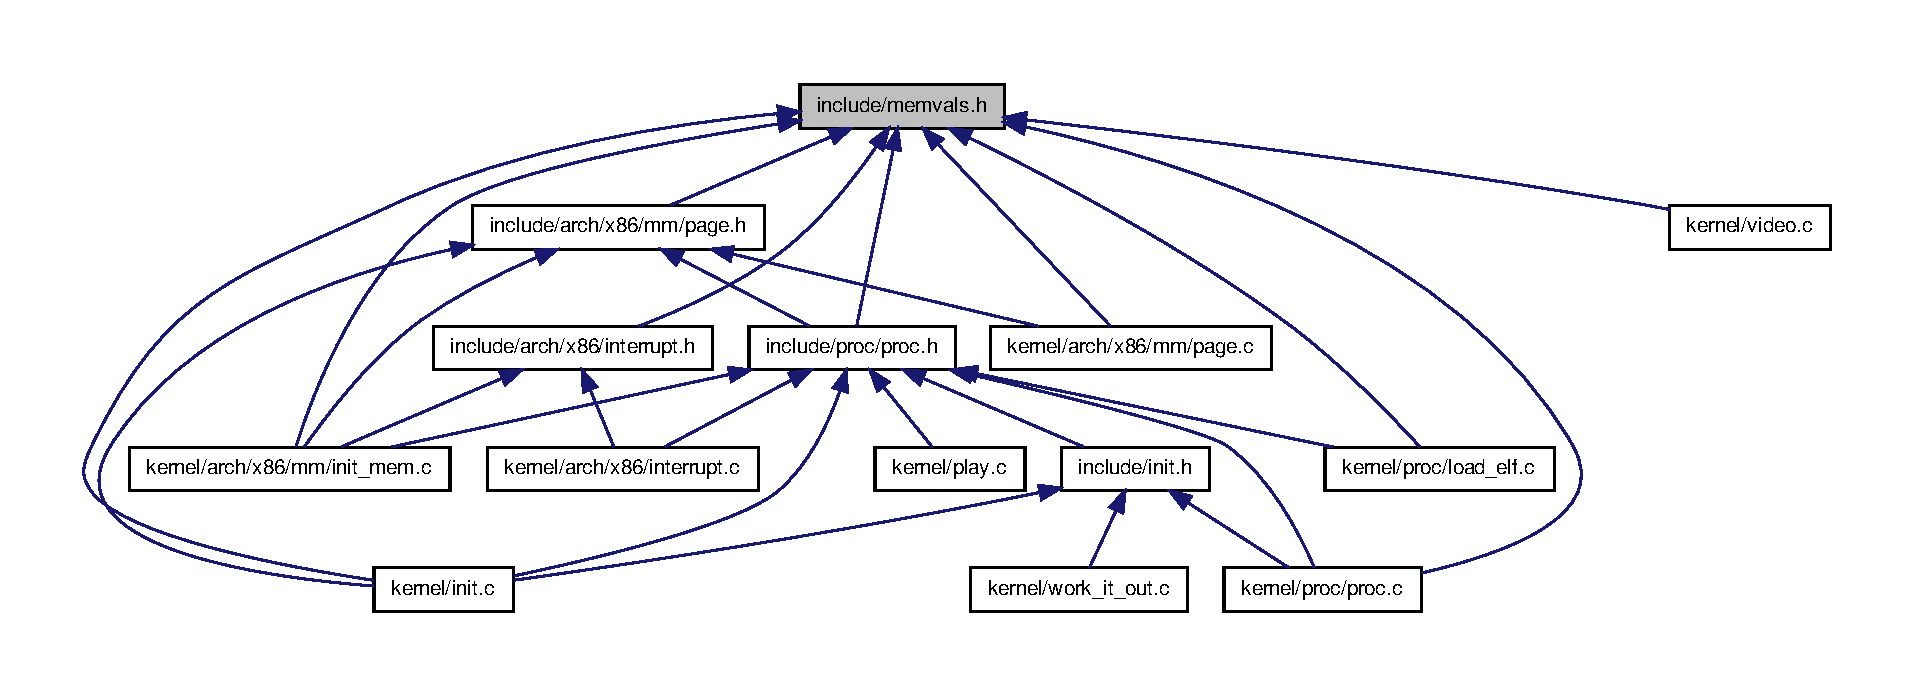
\includegraphics[width=350pt]{memvals_8h__dep__incl}
\end{center}
\end{figure}
\subsection*{\-Data \-Structures}
\begin{DoxyCompactItemize}
\item 
struct \hyperlink{structSegdesc}{\-Segdesc}
\item 
struct \hyperlink{structGdtdesc}{\-Gdtdesc}
\end{DoxyCompactItemize}
\subsection*{\-Defines}
\begin{DoxyCompactItemize}
\item 
\#define \hyperlink{memvals_8h_a3339ed3317bf1983a963ec00b5e6920e}{\-S\-E\-G\-A\-C\-S\-\_\-\-R\-W}~0x2	/$\ast$ Read and write flag Read for code segments and write for data segments $\ast$/
\item 
\#define \hyperlink{memvals_8h_a320426c604cdecc5a193134703d15864}{\-S\-E\-G\-A\-C\-S\-\_\-\-X}~0x8	/$\ast$ The Executable flag $\ast$/
\item 
\#define \hyperlink{memvals_8h_a14ac70ce8b1d2b8947785bb263f34dff}{\-S\-E\-G\-A\-C\-S\-\_\-\-D}
\item 
\#define \hyperlink{memvals_8h_ac0df0c9e3291f13ac316e36566673ee5}{\-S\-E\-G\-A\-C\-S\-\_\-\-U\-S\-R}~0x60
\item 
\#define \hyperlink{memvals_8h_a594f82f31d1ed7189ad21c3af3279269}{\-S\-E\-G\-\_\-\-N\-U\-L\-L}~(struct \hyperlink{structSegdesc}{\-Segdesc})\{0,0,0,0,0,0,0\}
\item 
\#define \hyperlink{memvals_8h_a51cd335eb7b3c2775b28995bc5a8b9a4}{\-S\-E\-G\-M\-E\-N\-T}(limit, \hyperlink{memvals_8h_a0523cedff47e2441fc198b7770ec5d3f}{base}, access)
\item 
\#define \hyperlink{memvals_8h_afa15977c771e531ebd3f3a5c2563ce16}{\-E\-X\-T\-M\-E\-M}~0x100000
\item 
\#define \hyperlink{memvals_8h_afaaefef20f05b195fe951996639d6e0b}{\-P\-A\-G\-E\-S\-Z}~0x1000
\item 
\#define \hyperlink{memvals_8h_afa3787ef60f1ab1900e4155a69c294e7}{\-P\-A\-G\-E\-L\-G}~0x\-C
\item 
\#define \hyperlink{memvals_8h_a2ae6c608093b58db8aeb7a55afa6ced4}{\-P\-A\-G\-E\-C\-N\-T}~0x400
\item 
\#define \hyperlink{memvals_8h_a5f6a8c03818b17c32a2fbc2151cee288}{\-P\-A\-G\-E\-T\-S\-Z}~(\hyperlink{memvals_8h_afaaefef20f05b195fe951996639d6e0b}{\-P\-A\-G\-E\-S\-Z}$\ast$\hyperlink{memvals_8h_a2ae6c608093b58db8aeb7a55afa6ced4}{\-P\-A\-G\-E\-C\-N\-T})
\item 
\#define \hyperlink{memvals_8h_ad72dec5e3e9cbc32c38253c447e875ad}{\-K\-E\-R\-N\-E\-L\-\_\-\-A\-D\-D\-R}~0x\-F0000000
\item 
\#define \hyperlink{memvals_8h_a23c7f2f55680575f333c26044f6097cb}{\-K\-E\-R\-N\-E\-L\-\_\-\-S\-T\-A\-C\-K}~\hyperlink{memvals_8h_afaaefef20f05b195fe951996639d6e0b}{\-P\-A\-G\-E\-S\-Z}$\ast$8
\item 
\#define \hyperlink{memvals_8h_ace568adaf7e532683e563d7cbcfe6328}{\-V\-I\-R\-T\-P\-G\-T}~(\hyperlink{memvals_8h_ad72dec5e3e9cbc32c38253c447e875ad}{\-K\-E\-R\-N\-E\-L\-\_\-\-A\-D\-D\-R} -\/ \hyperlink{memvals_8h_a5f6a8c03818b17c32a2fbc2151cee288}{\-P\-A\-G\-E\-T\-S\-Z})
\item 
\#define \hyperlink{memvals_8h_aac7f7736d8372772fdc018238ddd255d}{\-K\-E\-R\-N\-E\-L\-\_\-\-S\-T\-A\-C\-K\-\_\-\-T\-O\-P}~\hyperlink{memvals_8h_ace568adaf7e532683e563d7cbcfe6328}{\-V\-I\-R\-T\-P\-G\-T}
\item 
\#define \hyperlink{memvals_8h_a39d3d196a74d68f2386ac220de11c62d}{\-U\-S\-E\-R\-E\-N\-D}~(\hyperlink{memvals_8h_ace568adaf7e532683e563d7cbcfe6328}{\-V\-I\-R\-T\-P\-G\-T} -\/ \hyperlink{memvals_8h_a5f6a8c03818b17c32a2fbc2151cee288}{\-P\-A\-G\-E\-T\-S\-Z})
\item 
\#define \hyperlink{memvals_8h_a071ef09fc45a890d9b9a44a5f983ef65}{\-U\-S\-E\-R\-V\-I\-R\-T\-P\-G\-T}~(\hyperlink{memvals_8h_a39d3d196a74d68f2386ac220de11c62d}{\-U\-S\-E\-R\-E\-N\-D} -\/ \hyperlink{memvals_8h_a5f6a8c03818b17c32a2fbc2151cee288}{\-P\-A\-G\-E\-T\-S\-Z})
\item 
\#define \hyperlink{memvals_8h_a626f3751ebabc3f61df0d77cbbe536ae}{\-U\-S\-E\-R\-P\-A\-G\-E\-S}~(\hyperlink{memvals_8h_a071ef09fc45a890d9b9a44a5f983ef65}{\-U\-S\-E\-R\-V\-I\-R\-T\-P\-G\-T} -\/ \hyperlink{memvals_8h_a5f6a8c03818b17c32a2fbc2151cee288}{\-P\-A\-G\-E\-T\-S\-Z})
\item 
\#define \hyperlink{memvals_8h_a6220d966059baa20fc62479d1b620b37}{\-P\-R\-O\-C\-\_\-\-L\-I\-S\-T}~(\hyperlink{memvals_8h_a626f3751ebabc3f61df0d77cbbe536ae}{\-U\-S\-E\-R\-P\-A\-G\-E\-S} -\/ \hyperlink{memvals_8h_a5f6a8c03818b17c32a2fbc2151cee288}{\-P\-A\-G\-E\-T\-S\-Z})
\item 
\#define \hyperlink{memvals_8h_ae3ae3cfc7cee7569379146d2f31a9f9f}{\-U\-S\-E\-R\-S\-T\-A\-R\-T}~(\hyperlink{memvals_8h_a6220d966059baa20fc62479d1b620b37}{\-P\-R\-O\-C\-\_\-\-L\-I\-S\-T})
\item 
\#define \hyperlink{memvals_8h_a30a99faf9b563bfbd6bb3889f313673c}{\-U\-S\-E\-R\-S\-T\-A\-C\-K\-\_\-\-T\-O\-P}~(\hyperlink{memvals_8h_ae3ae3cfc7cee7569379146d2f31a9f9f}{\-U\-S\-E\-R\-S\-T\-A\-R\-T} -\/ 2$\ast$\hyperlink{memvals_8h_afaaefef20f05b195fe951996639d6e0b}{\-P\-A\-G\-E\-S\-Z})
\item 
\#define \hyperlink{memvals_8h_ae19a309f4177d8849b5ebe8ebe7d76c9}{\-U\-S\-E\-R\-S\-P\-A\-C\-E\-S\-T\-A\-R\-T}~0\-X\-E\-E800000
\item 
\#define \hyperlink{memvals_8h_adcb9a0e28614fc06bf37d46dfe40ae99}{\-P\-A}(va)
\item 
\#define \hyperlink{memvals_8h_a8d55351437a0f35a5b3091d8acf6fa42}{\-I\-O\-P\-H\-Y\-M\-E\-M}~0x0\-A0000
\item 
\#define \hyperlink{memvals_8h_a1841fd1a462d245d8c73dce55e2f45da}{\-K\-B}~0x400
\item 
\#define \hyperlink{memvals_8h_aa6b38d492364d98453284934ed7caee9}{\-M\-B}~\hyperlink{memvals_8h_a1841fd1a462d245d8c73dce55e2f45da}{\-K\-B}$\ast$\hyperlink{memvals_8h_a1841fd1a462d245d8c73dce55e2f45da}{\-K\-B}
\item 
\#define \hyperlink{memvals_8h_a44172ac633c517cb4c9e278cef36b000}{\-G\-B}~\hyperlink{memvals_8h_aa6b38d492364d98453284934ed7caee9}{\-M\-B}$\ast$\hyperlink{memvals_8h_a1841fd1a462d245d8c73dce55e2f45da}{\-K\-B}
\end{DoxyCompactItemize}
\subsection*{\-Functions}
\begin{DoxyCompactItemize}
\item 
struct \hyperlink{structGdtdesc}{\-Gdtdesc} \hyperlink{memvals_8h_a038c990262fc385e807818a59ff8e25f}{\-\_\-\-\_\-attribute\-\_\-\-\_\-} ((packed))
\end{DoxyCompactItemize}
\subsection*{\-Variables}
\begin{DoxyCompactItemize}
\item 
\hyperlink{types_8h_a273cf69d639a59973b6019625df33e30}{uint16\-\_\-t} \hyperlink{memvals_8h_aaba88b24a21a6c70c895c0d55f4a69a0}{size}
\item 
\hyperlink{types_8h_a435d1572bf3f880d55459d9805097f62}{uint32\-\_\-t} \hyperlink{memvals_8h_a0523cedff47e2441fc198b7770ec5d3f}{base}
\end{DoxyCompactItemize}


\subsection{\-Define \-Documentation}
\hypertarget{memvals_8h_afa15977c771e531ebd3f3a5c2563ce16}{\index{memvals.\-h@{memvals.\-h}!\-E\-X\-T\-M\-E\-M@{\-E\-X\-T\-M\-E\-M}}
\index{\-E\-X\-T\-M\-E\-M@{\-E\-X\-T\-M\-E\-M}!memvals.h@{memvals.\-h}}
\subsubsection[{\-E\-X\-T\-M\-E\-M}]{\setlength{\rightskip}{0pt plus 5cm}\#define {\bf \-E\-X\-T\-M\-E\-M}~0x100000}}\label{memvals_8h_afa15977c771e531ebd3f3a5c2563ce16}


\-Definition at line 83 of file memvals.\-h.

\hypertarget{memvals_8h_a44172ac633c517cb4c9e278cef36b000}{\index{memvals.\-h@{memvals.\-h}!\-G\-B@{\-G\-B}}
\index{\-G\-B@{\-G\-B}!memvals.h@{memvals.\-h}}
\subsubsection[{\-G\-B}]{\setlength{\rightskip}{0pt plus 5cm}\#define {\bf \-G\-B}~{\bf \-M\-B}$\ast${\bf \-K\-B}}}\label{memvals_8h_a44172ac633c517cb4c9e278cef36b000}


\-Definition at line 120 of file memvals.\-h.

\hypertarget{memvals_8h_a8d55351437a0f35a5b3091d8acf6fa42}{\index{memvals.\-h@{memvals.\-h}!\-I\-O\-P\-H\-Y\-M\-E\-M@{\-I\-O\-P\-H\-Y\-M\-E\-M}}
\index{\-I\-O\-P\-H\-Y\-M\-E\-M@{\-I\-O\-P\-H\-Y\-M\-E\-M}!memvals.h@{memvals.\-h}}
\subsubsection[{\-I\-O\-P\-H\-Y\-M\-E\-M}]{\setlength{\rightskip}{0pt plus 5cm}\#define {\bf \-I\-O\-P\-H\-Y\-M\-E\-M}~0x0\-A0000}}\label{memvals_8h_a8d55351437a0f35a5b3091d8acf6fa42}
\-Paging 

\-Definition at line 114 of file memvals.\-h.

\hypertarget{memvals_8h_a1841fd1a462d245d8c73dce55e2f45da}{\index{memvals.\-h@{memvals.\-h}!\-K\-B@{\-K\-B}}
\index{\-K\-B@{\-K\-B}!memvals.h@{memvals.\-h}}
\subsubsection[{\-K\-B}]{\setlength{\rightskip}{0pt plus 5cm}\#define {\bf \-K\-B}~0x400}}\label{memvals_8h_a1841fd1a462d245d8c73dce55e2f45da}


\-Definition at line 118 of file memvals.\-h.

\hypertarget{memvals_8h_ad72dec5e3e9cbc32c38253c447e875ad}{\index{memvals.\-h@{memvals.\-h}!\-K\-E\-R\-N\-E\-L\-\_\-\-A\-D\-D\-R@{\-K\-E\-R\-N\-E\-L\-\_\-\-A\-D\-D\-R}}
\index{\-K\-E\-R\-N\-E\-L\-\_\-\-A\-D\-D\-R@{\-K\-E\-R\-N\-E\-L\-\_\-\-A\-D\-D\-R}!memvals.h@{memvals.\-h}}
\subsubsection[{\-K\-E\-R\-N\-E\-L\-\_\-\-A\-D\-D\-R}]{\setlength{\rightskip}{0pt plus 5cm}\#define {\bf \-K\-E\-R\-N\-E\-L\-\_\-\-A\-D\-D\-R}~0x\-F0000000}}\label{memvals_8h_ad72dec5e3e9cbc32c38253c447e875ad}


\-Definition at line 88 of file memvals.\-h.

\hypertarget{memvals_8h_a23c7f2f55680575f333c26044f6097cb}{\index{memvals.\-h@{memvals.\-h}!\-K\-E\-R\-N\-E\-L\-\_\-\-S\-T\-A\-C\-K@{\-K\-E\-R\-N\-E\-L\-\_\-\-S\-T\-A\-C\-K}}
\index{\-K\-E\-R\-N\-E\-L\-\_\-\-S\-T\-A\-C\-K@{\-K\-E\-R\-N\-E\-L\-\_\-\-S\-T\-A\-C\-K}!memvals.h@{memvals.\-h}}
\subsubsection[{\-K\-E\-R\-N\-E\-L\-\_\-\-S\-T\-A\-C\-K}]{\setlength{\rightskip}{0pt plus 5cm}\#define {\bf \-K\-E\-R\-N\-E\-L\-\_\-\-S\-T\-A\-C\-K}~{\bf \-P\-A\-G\-E\-S\-Z}$\ast$8}}\label{memvals_8h_a23c7f2f55680575f333c26044f6097cb}


\-Definition at line 89 of file memvals.\-h.

\hypertarget{memvals_8h_aac7f7736d8372772fdc018238ddd255d}{\index{memvals.\-h@{memvals.\-h}!\-K\-E\-R\-N\-E\-L\-\_\-\-S\-T\-A\-C\-K\-\_\-\-T\-O\-P@{\-K\-E\-R\-N\-E\-L\-\_\-\-S\-T\-A\-C\-K\-\_\-\-T\-O\-P}}
\index{\-K\-E\-R\-N\-E\-L\-\_\-\-S\-T\-A\-C\-K\-\_\-\-T\-O\-P@{\-K\-E\-R\-N\-E\-L\-\_\-\-S\-T\-A\-C\-K\-\_\-\-T\-O\-P}!memvals.h@{memvals.\-h}}
\subsubsection[{\-K\-E\-R\-N\-E\-L\-\_\-\-S\-T\-A\-C\-K\-\_\-\-T\-O\-P}]{\setlength{\rightskip}{0pt plus 5cm}\#define {\bf \-K\-E\-R\-N\-E\-L\-\_\-\-S\-T\-A\-C\-K\-\_\-\-T\-O\-P}~{\bf \-V\-I\-R\-T\-P\-G\-T}}}\label{memvals_8h_aac7f7736d8372772fdc018238ddd255d}


\-Definition at line 91 of file memvals.\-h.

\hypertarget{memvals_8h_aa6b38d492364d98453284934ed7caee9}{\index{memvals.\-h@{memvals.\-h}!\-M\-B@{\-M\-B}}
\index{\-M\-B@{\-M\-B}!memvals.h@{memvals.\-h}}
\subsubsection[{\-M\-B}]{\setlength{\rightskip}{0pt plus 5cm}\#define {\bf \-M\-B}~{\bf \-K\-B}$\ast${\bf \-K\-B}}}\label{memvals_8h_aa6b38d492364d98453284934ed7caee9}


\-Definition at line 119 of file memvals.\-h.

\hypertarget{memvals_8h_adcb9a0e28614fc06bf37d46dfe40ae99}{\index{memvals.\-h@{memvals.\-h}!\-P\-A@{\-P\-A}}
\index{\-P\-A@{\-P\-A}!memvals.h@{memvals.\-h}}
\subsubsection[{\-P\-A}]{\setlength{\rightskip}{0pt plus 5cm}\#define {\bf \-P\-A}(
\begin{DoxyParamCaption}
\item[{}]{va}
\end{DoxyParamCaption}
)}}\label{memvals_8h_adcb9a0e28614fc06bf37d46dfe40ae99}
{\bfseries \-Value\-:}
\begin{DoxyCode}
({\
        uint32_t pa = (uint32_t) va;\
        pa-KERNEL_ADDR;\
})
\end{DoxyCode}


\-Definition at line 103 of file memvals.\-h.

\hypertarget{memvals_8h_a2ae6c608093b58db8aeb7a55afa6ced4}{\index{memvals.\-h@{memvals.\-h}!\-P\-A\-G\-E\-C\-N\-T@{\-P\-A\-G\-E\-C\-N\-T}}
\index{\-P\-A\-G\-E\-C\-N\-T@{\-P\-A\-G\-E\-C\-N\-T}!memvals.h@{memvals.\-h}}
\subsubsection[{\-P\-A\-G\-E\-C\-N\-T}]{\setlength{\rightskip}{0pt plus 5cm}\#define {\bf \-P\-A\-G\-E\-C\-N\-T}~0x400}}\label{memvals_8h_a2ae6c608093b58db8aeb7a55afa6ced4}


\-Definition at line 86 of file memvals.\-h.

\hypertarget{memvals_8h_afa3787ef60f1ab1900e4155a69c294e7}{\index{memvals.\-h@{memvals.\-h}!\-P\-A\-G\-E\-L\-G@{\-P\-A\-G\-E\-L\-G}}
\index{\-P\-A\-G\-E\-L\-G@{\-P\-A\-G\-E\-L\-G}!memvals.h@{memvals.\-h}}
\subsubsection[{\-P\-A\-G\-E\-L\-G}]{\setlength{\rightskip}{0pt plus 5cm}\#define {\bf \-P\-A\-G\-E\-L\-G}~0x\-C}}\label{memvals_8h_afa3787ef60f1ab1900e4155a69c294e7}


\-Definition at line 85 of file memvals.\-h.

\hypertarget{memvals_8h_afaaefef20f05b195fe951996639d6e0b}{\index{memvals.\-h@{memvals.\-h}!\-P\-A\-G\-E\-S\-Z@{\-P\-A\-G\-E\-S\-Z}}
\index{\-P\-A\-G\-E\-S\-Z@{\-P\-A\-G\-E\-S\-Z}!memvals.h@{memvals.\-h}}
\subsubsection[{\-P\-A\-G\-E\-S\-Z}]{\setlength{\rightskip}{0pt plus 5cm}\#define {\bf \-P\-A\-G\-E\-S\-Z}~0x1000}}\label{memvals_8h_afaaefef20f05b195fe951996639d6e0b}


\-Definition at line 84 of file memvals.\-h.

\hypertarget{memvals_8h_a5f6a8c03818b17c32a2fbc2151cee288}{\index{memvals.\-h@{memvals.\-h}!\-P\-A\-G\-E\-T\-S\-Z@{\-P\-A\-G\-E\-T\-S\-Z}}
\index{\-P\-A\-G\-E\-T\-S\-Z@{\-P\-A\-G\-E\-T\-S\-Z}!memvals.h@{memvals.\-h}}
\subsubsection[{\-P\-A\-G\-E\-T\-S\-Z}]{\setlength{\rightskip}{0pt plus 5cm}\#define {\bf \-P\-A\-G\-E\-T\-S\-Z}~({\bf \-P\-A\-G\-E\-S\-Z}$\ast${\bf \-P\-A\-G\-E\-C\-N\-T})}}\label{memvals_8h_a5f6a8c03818b17c32a2fbc2151cee288}


\-Definition at line 87 of file memvals.\-h.

\hypertarget{memvals_8h_a6220d966059baa20fc62479d1b620b37}{\index{memvals.\-h@{memvals.\-h}!\-P\-R\-O\-C\-\_\-\-L\-I\-S\-T@{\-P\-R\-O\-C\-\_\-\-L\-I\-S\-T}}
\index{\-P\-R\-O\-C\-\_\-\-L\-I\-S\-T@{\-P\-R\-O\-C\-\_\-\-L\-I\-S\-T}!memvals.h@{memvals.\-h}}
\subsubsection[{\-P\-R\-O\-C\-\_\-\-L\-I\-S\-T}]{\setlength{\rightskip}{0pt plus 5cm}\#define {\bf \-P\-R\-O\-C\-\_\-\-L\-I\-S\-T}~({\bf \-U\-S\-E\-R\-P\-A\-G\-E\-S} -\/ {\bf \-P\-A\-G\-E\-T\-S\-Z})}}\label{memvals_8h_a6220d966059baa20fc62479d1b620b37}


\-Definition at line 96 of file memvals.\-h.

\hypertarget{memvals_8h_a594f82f31d1ed7189ad21c3af3279269}{\index{memvals.\-h@{memvals.\-h}!\-S\-E\-G\-\_\-\-N\-U\-L\-L@{\-S\-E\-G\-\_\-\-N\-U\-L\-L}}
\index{\-S\-E\-G\-\_\-\-N\-U\-L\-L@{\-S\-E\-G\-\_\-\-N\-U\-L\-L}!memvals.h@{memvals.\-h}}
\subsubsection[{\-S\-E\-G\-\_\-\-N\-U\-L\-L}]{\setlength{\rightskip}{0pt plus 5cm}\#define {\bf \-S\-E\-G\-\_\-\-N\-U\-L\-L}~(struct {\bf \-Segdesc})\{0,0,0,0,0,0,0\}}}\label{memvals_8h_a594f82f31d1ed7189ad21c3af3279269}


\-Definition at line 67 of file memvals.\-h.

\hypertarget{memvals_8h_a14ac70ce8b1d2b8947785bb263f34dff}{\index{memvals.\-h@{memvals.\-h}!\-S\-E\-G\-A\-C\-S\-\_\-\-D@{\-S\-E\-G\-A\-C\-S\-\_\-\-D}}
\index{\-S\-E\-G\-A\-C\-S\-\_\-\-D@{\-S\-E\-G\-A\-C\-S\-\_\-\-D}!memvals.h@{memvals.\-h}}
\subsubsection[{\-S\-E\-G\-A\-C\-S\-\_\-\-D}]{\setlength{\rightskip}{0pt plus 5cm}\#define {\bf \-S\-E\-G\-A\-C\-S\-\_\-\-D}}}\label{memvals_8h_a14ac70ce8b1d2b8947785bb263f34dff}
{\bfseries \-Value\-:}
\begin{DoxyCode}
0x4     /* growing down segment for data segments and means that this segments
       can be
                                        Executed from the user applications
       "Low Privilege" */
\end{DoxyCode}


\-Definition at line 54 of file memvals.\-h.

\hypertarget{memvals_8h_a3339ed3317bf1983a963ec00b5e6920e}{\index{memvals.\-h@{memvals.\-h}!\-S\-E\-G\-A\-C\-S\-\_\-\-R\-W@{\-S\-E\-G\-A\-C\-S\-\_\-\-R\-W}}
\index{\-S\-E\-G\-A\-C\-S\-\_\-\-R\-W@{\-S\-E\-G\-A\-C\-S\-\_\-\-R\-W}!memvals.h@{memvals.\-h}}
\subsubsection[{\-S\-E\-G\-A\-C\-S\-\_\-\-R\-W}]{\setlength{\rightskip}{0pt plus 5cm}\#define {\bf \-S\-E\-G\-A\-C\-S\-\_\-\-R\-W}~0x2	/$\ast$ Read and write flag Read for code segments and write for data segments $\ast$/}}\label{memvals_8h_a3339ed3317bf1983a963ec00b5e6920e}


\-Definition at line 52 of file memvals.\-h.

\hypertarget{memvals_8h_ac0df0c9e3291f13ac316e36566673ee5}{\index{memvals.\-h@{memvals.\-h}!\-S\-E\-G\-A\-C\-S\-\_\-\-U\-S\-R@{\-S\-E\-G\-A\-C\-S\-\_\-\-U\-S\-R}}
\index{\-S\-E\-G\-A\-C\-S\-\_\-\-U\-S\-R@{\-S\-E\-G\-A\-C\-S\-\_\-\-U\-S\-R}!memvals.h@{memvals.\-h}}
\subsubsection[{\-S\-E\-G\-A\-C\-S\-\_\-\-U\-S\-R}]{\setlength{\rightskip}{0pt plus 5cm}\#define {\bf \-S\-E\-G\-A\-C\-S\-\_\-\-U\-S\-R}~0x60}}\label{memvals_8h_ac0df0c9e3291f13ac316e36566673ee5}


\-Definition at line 55 of file memvals.\-h.

\hypertarget{memvals_8h_a320426c604cdecc5a193134703d15864}{\index{memvals.\-h@{memvals.\-h}!\-S\-E\-G\-A\-C\-S\-\_\-\-X@{\-S\-E\-G\-A\-C\-S\-\_\-\-X}}
\index{\-S\-E\-G\-A\-C\-S\-\_\-\-X@{\-S\-E\-G\-A\-C\-S\-\_\-\-X}!memvals.h@{memvals.\-h}}
\subsubsection[{\-S\-E\-G\-A\-C\-S\-\_\-\-X}]{\setlength{\rightskip}{0pt plus 5cm}\#define {\bf \-S\-E\-G\-A\-C\-S\-\_\-\-X}~0x8	/$\ast$ The Executable flag $\ast$/}}\label{memvals_8h_a320426c604cdecc5a193134703d15864}


\-Definition at line 53 of file memvals.\-h.

\hypertarget{memvals_8h_a51cd335eb7b3c2775b28995bc5a8b9a4}{\index{memvals.\-h@{memvals.\-h}!\-S\-E\-G\-M\-E\-N\-T@{\-S\-E\-G\-M\-E\-N\-T}}
\index{\-S\-E\-G\-M\-E\-N\-T@{\-S\-E\-G\-M\-E\-N\-T}!memvals.h@{memvals.\-h}}
\subsubsection[{\-S\-E\-G\-M\-E\-N\-T}]{\setlength{\rightskip}{0pt plus 5cm}\#define {\bf \-S\-E\-G\-M\-E\-N\-T}(
\begin{DoxyParamCaption}
\item[{}]{limit, }
\item[{}]{{\bf base}, }
\item[{}]{access}
\end{DoxyParamCaption}
)}}\label{memvals_8h_a51cd335eb7b3c2775b28995bc5a8b9a4}
{\bfseries \-Value\-:}
\begin{DoxyCode}
(struct Segdesc)\
        {\
        (limit>>12) & 0xFFFF,\
        (base) & 0xFFFF,\
        ((base)>>16) & 0xFF,\
        (access) | 0x90,\
        ((limit) >> 28),\
        0xC,\
        (base)>>24\
        }
\end{DoxyCode}


\-Definition at line 68 of file memvals.\-h.

\hypertarget{memvals_8h_a39d3d196a74d68f2386ac220de11c62d}{\index{memvals.\-h@{memvals.\-h}!\-U\-S\-E\-R\-E\-N\-D@{\-U\-S\-E\-R\-E\-N\-D}}
\index{\-U\-S\-E\-R\-E\-N\-D@{\-U\-S\-E\-R\-E\-N\-D}!memvals.h@{memvals.\-h}}
\subsubsection[{\-U\-S\-E\-R\-E\-N\-D}]{\setlength{\rightskip}{0pt plus 5cm}\#define {\bf \-U\-S\-E\-R\-E\-N\-D}~({\bf \-V\-I\-R\-T\-P\-G\-T} -\/ {\bf \-P\-A\-G\-E\-T\-S\-Z})}}\label{memvals_8h_a39d3d196a74d68f2386ac220de11c62d}


\-Definition at line 93 of file memvals.\-h.

\hypertarget{memvals_8h_a626f3751ebabc3f61df0d77cbbe536ae}{\index{memvals.\-h@{memvals.\-h}!\-U\-S\-E\-R\-P\-A\-G\-E\-S@{\-U\-S\-E\-R\-P\-A\-G\-E\-S}}
\index{\-U\-S\-E\-R\-P\-A\-G\-E\-S@{\-U\-S\-E\-R\-P\-A\-G\-E\-S}!memvals.h@{memvals.\-h}}
\subsubsection[{\-U\-S\-E\-R\-P\-A\-G\-E\-S}]{\setlength{\rightskip}{0pt plus 5cm}\#define {\bf \-U\-S\-E\-R\-P\-A\-G\-E\-S}~({\bf \-U\-S\-E\-R\-V\-I\-R\-T\-P\-G\-T} -\/ {\bf \-P\-A\-G\-E\-T\-S\-Z})}}\label{memvals_8h_a626f3751ebabc3f61df0d77cbbe536ae}


\-Definition at line 95 of file memvals.\-h.

\hypertarget{memvals_8h_ae19a309f4177d8849b5ebe8ebe7d76c9}{\index{memvals.\-h@{memvals.\-h}!\-U\-S\-E\-R\-S\-P\-A\-C\-E\-S\-T\-A\-R\-T@{\-U\-S\-E\-R\-S\-P\-A\-C\-E\-S\-T\-A\-R\-T}}
\index{\-U\-S\-E\-R\-S\-P\-A\-C\-E\-S\-T\-A\-R\-T@{\-U\-S\-E\-R\-S\-P\-A\-C\-E\-S\-T\-A\-R\-T}!memvals.h@{memvals.\-h}}
\subsubsection[{\-U\-S\-E\-R\-S\-P\-A\-C\-E\-S\-T\-A\-R\-T}]{\setlength{\rightskip}{0pt plus 5cm}\#define {\bf \-U\-S\-E\-R\-S\-P\-A\-C\-E\-S\-T\-A\-R\-T}~0\-X\-E\-E800000}}\label{memvals_8h_ae19a309f4177d8849b5ebe8ebe7d76c9}


\-Definition at line 101 of file memvals.\-h.

\hypertarget{memvals_8h_a30a99faf9b563bfbd6bb3889f313673c}{\index{memvals.\-h@{memvals.\-h}!\-U\-S\-E\-R\-S\-T\-A\-C\-K\-\_\-\-T\-O\-P@{\-U\-S\-E\-R\-S\-T\-A\-C\-K\-\_\-\-T\-O\-P}}
\index{\-U\-S\-E\-R\-S\-T\-A\-C\-K\-\_\-\-T\-O\-P@{\-U\-S\-E\-R\-S\-T\-A\-C\-K\-\_\-\-T\-O\-P}!memvals.h@{memvals.\-h}}
\subsubsection[{\-U\-S\-E\-R\-S\-T\-A\-C\-K\-\_\-\-T\-O\-P}]{\setlength{\rightskip}{0pt plus 5cm}\#define {\bf \-U\-S\-E\-R\-S\-T\-A\-C\-K\-\_\-\-T\-O\-P}~({\bf \-U\-S\-E\-R\-S\-T\-A\-R\-T} -\/ 2$\ast${\bf \-P\-A\-G\-E\-S\-Z})}}\label{memvals_8h_a30a99faf9b563bfbd6bb3889f313673c}


\-Definition at line 98 of file memvals.\-h.

\hypertarget{memvals_8h_ae3ae3cfc7cee7569379146d2f31a9f9f}{\index{memvals.\-h@{memvals.\-h}!\-U\-S\-E\-R\-S\-T\-A\-R\-T@{\-U\-S\-E\-R\-S\-T\-A\-R\-T}}
\index{\-U\-S\-E\-R\-S\-T\-A\-R\-T@{\-U\-S\-E\-R\-S\-T\-A\-R\-T}!memvals.h@{memvals.\-h}}
\subsubsection[{\-U\-S\-E\-R\-S\-T\-A\-R\-T}]{\setlength{\rightskip}{0pt plus 5cm}\#define {\bf \-U\-S\-E\-R\-S\-T\-A\-R\-T}~({\bf \-P\-R\-O\-C\-\_\-\-L\-I\-S\-T})}}\label{memvals_8h_ae3ae3cfc7cee7569379146d2f31a9f9f}


\-Definition at line 97 of file memvals.\-h.

\hypertarget{memvals_8h_a071ef09fc45a890d9b9a44a5f983ef65}{\index{memvals.\-h@{memvals.\-h}!\-U\-S\-E\-R\-V\-I\-R\-T\-P\-G\-T@{\-U\-S\-E\-R\-V\-I\-R\-T\-P\-G\-T}}
\index{\-U\-S\-E\-R\-V\-I\-R\-T\-P\-G\-T@{\-U\-S\-E\-R\-V\-I\-R\-T\-P\-G\-T}!memvals.h@{memvals.\-h}}
\subsubsection[{\-U\-S\-E\-R\-V\-I\-R\-T\-P\-G\-T}]{\setlength{\rightskip}{0pt plus 5cm}\#define {\bf \-U\-S\-E\-R\-V\-I\-R\-T\-P\-G\-T}~({\bf \-U\-S\-E\-R\-E\-N\-D} -\/ {\bf \-P\-A\-G\-E\-T\-S\-Z})}}\label{memvals_8h_a071ef09fc45a890d9b9a44a5f983ef65}


\-Definition at line 94 of file memvals.\-h.

\hypertarget{memvals_8h_ace568adaf7e532683e563d7cbcfe6328}{\index{memvals.\-h@{memvals.\-h}!\-V\-I\-R\-T\-P\-G\-T@{\-V\-I\-R\-T\-P\-G\-T}}
\index{\-V\-I\-R\-T\-P\-G\-T@{\-V\-I\-R\-T\-P\-G\-T}!memvals.h@{memvals.\-h}}
\subsubsection[{\-V\-I\-R\-T\-P\-G\-T}]{\setlength{\rightskip}{0pt plus 5cm}\#define {\bf \-V\-I\-R\-T\-P\-G\-T}~({\bf \-K\-E\-R\-N\-E\-L\-\_\-\-A\-D\-D\-R} -\/ {\bf \-P\-A\-G\-E\-T\-S\-Z})}}\label{memvals_8h_ace568adaf7e532683e563d7cbcfe6328}


\-Definition at line 90 of file memvals.\-h.



\subsection{\-Function \-Documentation}
\hypertarget{memvals_8h_a038c990262fc385e807818a59ff8e25f}{\index{memvals.\-h@{memvals.\-h}!\-\_\-\-\_\-attribute\-\_\-\-\_\-@{\-\_\-\-\_\-attribute\-\_\-\-\_\-}}
\index{\-\_\-\-\_\-attribute\-\_\-\-\_\-@{\-\_\-\-\_\-attribute\-\_\-\-\_\-}!memvals.h@{memvals.\-h}}
\subsubsection[{\-\_\-\-\_\-attribute\-\_\-\-\_\-}]{\setlength{\rightskip}{0pt plus 5cm}struct {\bf \-Gdtdesc} {\bf \-\_\-\-\_\-attribute\-\_\-\-\_\-} (
\begin{DoxyParamCaption}
\item[{(packed)}]{}
\end{DoxyParamCaption}
)}}\label{memvals_8h_a038c990262fc385e807818a59ff8e25f}


\subsection{\-Variable \-Documentation}
\hypertarget{memvals_8h_a0523cedff47e2441fc198b7770ec5d3f}{\index{memvals.\-h@{memvals.\-h}!base@{base}}
\index{base@{base}!memvals.h@{memvals.\-h}}
\subsubsection[{base}]{\setlength{\rightskip}{0pt plus 5cm}{\bf uint32\-\_\-t} {\bf base}}}\label{memvals_8h_a0523cedff47e2441fc198b7770ec5d3f}


\-Definition at line 52 of file memvals.\-h.

\hypertarget{memvals_8h_aaba88b24a21a6c70c895c0d55f4a69a0}{\index{memvals.\-h@{memvals.\-h}!size@{size}}
\index{size@{size}!memvals.h@{memvals.\-h}}
\subsubsection[{size}]{\setlength{\rightskip}{0pt plus 5cm}{\bf uint16\-\_\-t} {\bf size}}}\label{memvals_8h_aaba88b24a21a6c70c895c0d55f4a69a0}


\-Definition at line 51 of file memvals.\-h.


\hypertarget{proc_8h}{\section{include/proc/proc.h \-File \-Reference}
\label{proc_8h}\index{include/proc/proc.\-h@{include/proc/proc.\-h}}
}
{\ttfamily \#include $<$arch/x86/cpu\-\_\-state.\-h$>$}\*
{\ttfamily \#include $<$memvals.\-h$>$}\*
{\ttfamily \#include $<$structs/queue.\-h$>$}\*
{\ttfamily \#include $<$arch/x86/mm/page.\-h$>$}\*
\-Include dependency graph for proc.\-h\-:\nopagebreak
\begin{figure}[H]
\begin{center}
\leavevmode
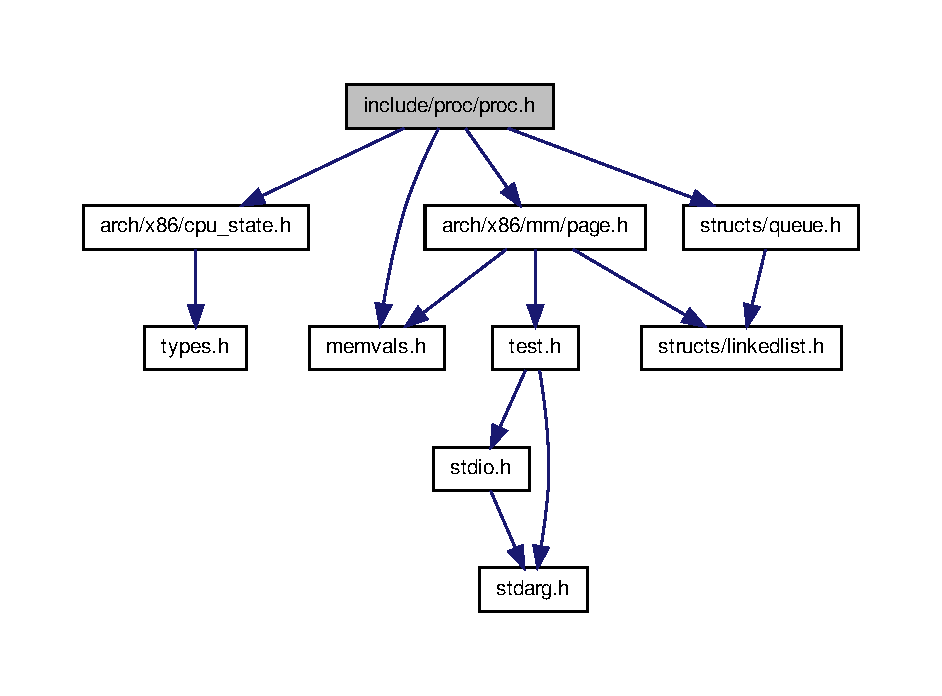
\includegraphics[width=350pt]{proc_8h__incl}
\end{center}
\end{figure}
\-This graph shows which files directly or indirectly include this file\-:\nopagebreak
\begin{figure}[H]
\begin{center}
\leavevmode
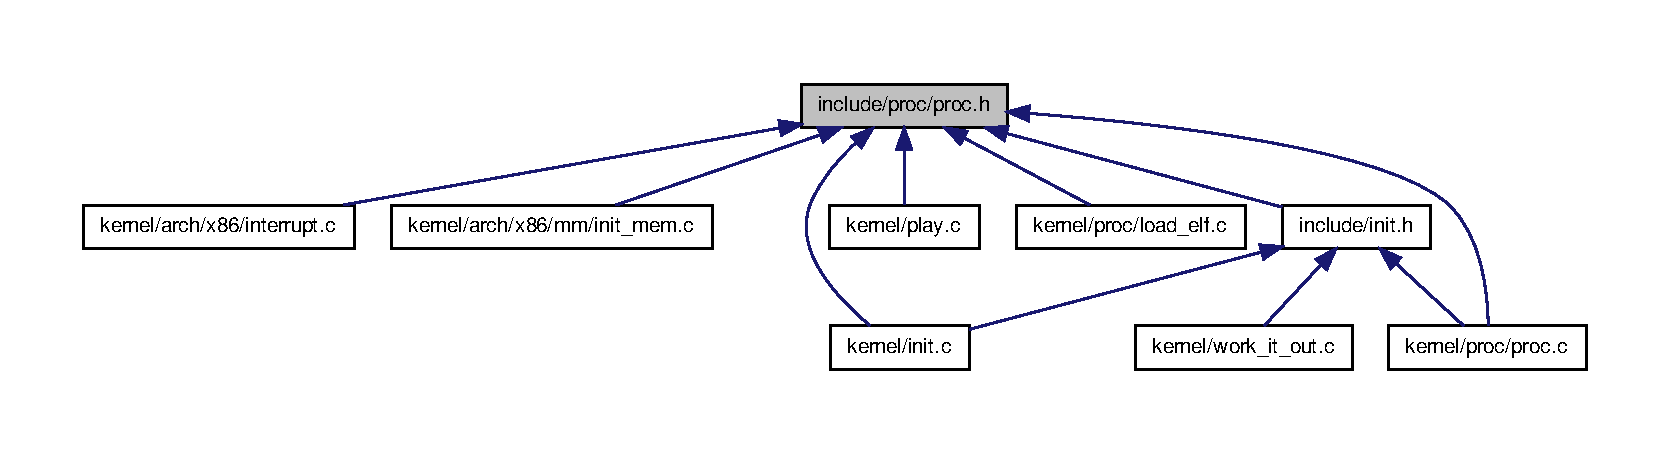
\includegraphics[width=350pt]{proc_8h__dep__incl}
\end{center}
\end{figure}
\subsection*{\-Data \-Structures}
\begin{DoxyCompactItemize}
\item 
struct \hyperlink{structproc}{proc}
\end{DoxyCompactItemize}
\subsection*{\-Defines}
\begin{DoxyCompactItemize}
\item 
\#define \hyperlink{proc_8h_a0e92bfcd9e51ca39bbebc3dfb9c16014}{\-M\-A\-X\-\_\-\-P\-R\-O\-C\-S}~256
\item 
\#define \hyperlink{proc_8h_a343751858d398e59d69b625d6593c288}{\-M\-A\-X\-\_\-\-P\-R\-O\-C\-\_\-\-N\-A\-M\-E}~128
\item 
\#define \hyperlink{proc_8h_a7ccc5ca21a66634195c2d9964c7817e8}{\-R\-U\-N\-N\-A\-B\-L\-E}~0
\item 
\#define \hyperlink{proc_8h_afca3664b6210cca51d6b7cc0ed9a884a}{\-P\-R\-O\-C\-\_\-\-E\-M\-P\-T\-Y}~0x1
\item 
\#define \hyperlink{proc_8h_a576996404555949ca922818a968d758d}{\-N\-O\-N\-\_\-\-R\-U\-N\-N\-A\-B\-L\-E}~0x2
\item 
\#define \hyperlink{proc_8h_a53c43501315a81999360575361f512b5}{\-P\-R\-O\-C\-\_\-\-T\-A\-B\-L\-E\-\_\-\-S\-I\-Z\-E}~\hyperlink{types_8h_a7a4ba4f2dbc3879306d8518c2670dd77}{\-R\-O\-U\-N\-D\-\_\-\-U\-P}(\hyperlink{proc_8h_a0e92bfcd9e51ca39bbebc3dfb9c16014}{\-M\-A\-X\-\_\-\-P\-R\-O\-C\-S} $\ast$ sizeof(struct \hyperlink{structproc}{proc}), \hyperlink{memvals_8h_afaaefef20f05b195fe951996639d6e0b}{\-P\-A\-G\-E\-S\-Z})
\end{DoxyCompactItemize}
\subsection*{\-Typedefs}
\begin{DoxyCompactItemize}
\item 
typedef struct \hyperlink{structproc}{proc} \hyperlink{proc_8h_abcae78bfd085fccd601f7cc568946453}{proc\-\_\-t}
\end{DoxyCompactItemize}
\subsection*{\-Functions}
\begin{DoxyCompactItemize}
\item 
\hyperlink{proc_8h_a07939ecde6cf51540dcf77e9c2c0098c}{\-L\-I\-S\-T\-\_\-\-H\-E\-A\-D} (\-Proc\-\_\-\-List, \hyperlink{structproc}{proc})
\item 
\hyperlink{proc_8h_abc4ce76c5721dbfcb7b522b97e1474c0}{\-L\-I\-F\-O\-\_\-\-H\-E\-A\-D} (\-Proc\-\_\-\-Lifo, \hyperlink{structproc}{proc})
\item 
void \hyperlink{proc_8h_a7a86f136018ec12ba764d8ecc13ee403}{init\-\_\-proc\-\_\-table} (void)
\item 
void \hyperlink{proc_8h_a1dbb2fb41967cafc4ef1e7ecc04002a0}{switch\-\_\-address\-\_\-space} (\hyperlink{proc_8h_abcae78bfd085fccd601f7cc568946453}{proc\-\_\-t} $\ast$)
\item 
\hyperlink{types_8h_a435d1572bf3f880d55459d9805097f62}{uint32\-\_\-t} \hyperlink{proc_8h_a05cfdf014538d1fb554b180744bedb4e}{proc\-\_\-setup} (\hyperlink{proc_8h_abcae78bfd085fccd601f7cc568946453}{proc\-\_\-t} $\ast$$\ast$)
\item 
\hyperlink{types_8h_a435d1572bf3f880d55459d9805097f62}{uint32\-\_\-t} \hyperlink{proc_8h_a427dfd5d9cec71a53e4b1c9d52dc8a1c}{proc\-\_\-setup\-\_\-mem} (\hyperlink{proc_8h_abcae78bfd085fccd601f7cc568946453}{proc\-\_\-t} $\ast$)
\item 
void \hyperlink{proc_8h_a5786a19c8d7e97d107ad3e1c02c12b0d}{test\-\_\-lifo} (void)
\end{DoxyCompactItemize}
\subsection*{\-Variables}
\begin{DoxyCompactItemize}
\item 
\hyperlink{proc_8h_abcae78bfd085fccd601f7cc568946453}{proc\-\_\-t} $\ast$ \hyperlink{proc_8h_a432b7b292b7d2423daf04aceac8924e6}{proc\-\_\-table}
\item 
struct \-Proc\-\_\-\-Lifo \hyperlink{proc_8h_a7608dc18b85a71c7c6f32b45a8516d12}{running\-\_\-procs}
\end{DoxyCompactItemize}


\subsection{\-Define \-Documentation}
\hypertarget{proc_8h_a343751858d398e59d69b625d6593c288}{\index{proc.\-h@{proc.\-h}!\-M\-A\-X\-\_\-\-P\-R\-O\-C\-\_\-\-N\-A\-M\-E@{\-M\-A\-X\-\_\-\-P\-R\-O\-C\-\_\-\-N\-A\-M\-E}}
\index{\-M\-A\-X\-\_\-\-P\-R\-O\-C\-\_\-\-N\-A\-M\-E@{\-M\-A\-X\-\_\-\-P\-R\-O\-C\-\_\-\-N\-A\-M\-E}!proc.h@{proc.\-h}}
\subsubsection[{\-M\-A\-X\-\_\-\-P\-R\-O\-C\-\_\-\-N\-A\-M\-E}]{\setlength{\rightskip}{0pt plus 5cm}\#define {\bf \-M\-A\-X\-\_\-\-P\-R\-O\-C\-\_\-\-N\-A\-M\-E}~128}}\label{proc_8h_a343751858d398e59d69b625d6593c288}


\-Definition at line 18 of file proc.\-h.

\hypertarget{proc_8h_a0e92bfcd9e51ca39bbebc3dfb9c16014}{\index{proc.\-h@{proc.\-h}!\-M\-A\-X\-\_\-\-P\-R\-O\-C\-S@{\-M\-A\-X\-\_\-\-P\-R\-O\-C\-S}}
\index{\-M\-A\-X\-\_\-\-P\-R\-O\-C\-S@{\-M\-A\-X\-\_\-\-P\-R\-O\-C\-S}!proc.h@{proc.\-h}}
\subsubsection[{\-M\-A\-X\-\_\-\-P\-R\-O\-C\-S}]{\setlength{\rightskip}{0pt plus 5cm}\#define {\bf \-M\-A\-X\-\_\-\-P\-R\-O\-C\-S}~256}}\label{proc_8h_a0e92bfcd9e51ca39bbebc3dfb9c16014}
inclede/arch/x86/interrupt.\-h \-C\-A\-T\-Reloaded (\-C) \-Copyrights 2011 \href{http:/ecatreloaded.net}{\tt http\-:/ecatreloaded.\-net}

\begin{DoxyDate}{\-Date}
4 \-Oct, 2012 
\end{DoxyDate}


\-Definition at line 17 of file proc.\-h.

\hypertarget{proc_8h_a576996404555949ca922818a968d758d}{\index{proc.\-h@{proc.\-h}!\-N\-O\-N\-\_\-\-R\-U\-N\-N\-A\-B\-L\-E@{\-N\-O\-N\-\_\-\-R\-U\-N\-N\-A\-B\-L\-E}}
\index{\-N\-O\-N\-\_\-\-R\-U\-N\-N\-A\-B\-L\-E@{\-N\-O\-N\-\_\-\-R\-U\-N\-N\-A\-B\-L\-E}!proc.h@{proc.\-h}}
\subsubsection[{\-N\-O\-N\-\_\-\-R\-U\-N\-N\-A\-B\-L\-E}]{\setlength{\rightskip}{0pt plus 5cm}\#define {\bf \-N\-O\-N\-\_\-\-R\-U\-N\-N\-A\-B\-L\-E}~0x2}}\label{proc_8h_a576996404555949ca922818a968d758d}


\-Definition at line 22 of file proc.\-h.

\hypertarget{proc_8h_afca3664b6210cca51d6b7cc0ed9a884a}{\index{proc.\-h@{proc.\-h}!\-P\-R\-O\-C\-\_\-\-E\-M\-P\-T\-Y@{\-P\-R\-O\-C\-\_\-\-E\-M\-P\-T\-Y}}
\index{\-P\-R\-O\-C\-\_\-\-E\-M\-P\-T\-Y@{\-P\-R\-O\-C\-\_\-\-E\-M\-P\-T\-Y}!proc.h@{proc.\-h}}
\subsubsection[{\-P\-R\-O\-C\-\_\-\-E\-M\-P\-T\-Y}]{\setlength{\rightskip}{0pt plus 5cm}\#define {\bf \-P\-R\-O\-C\-\_\-\-E\-M\-P\-T\-Y}~0x1}}\label{proc_8h_afca3664b6210cca51d6b7cc0ed9a884a}


\-Definition at line 21 of file proc.\-h.

\hypertarget{proc_8h_a53c43501315a81999360575361f512b5}{\index{proc.\-h@{proc.\-h}!\-P\-R\-O\-C\-\_\-\-T\-A\-B\-L\-E\-\_\-\-S\-I\-Z\-E@{\-P\-R\-O\-C\-\_\-\-T\-A\-B\-L\-E\-\_\-\-S\-I\-Z\-E}}
\index{\-P\-R\-O\-C\-\_\-\-T\-A\-B\-L\-E\-\_\-\-S\-I\-Z\-E@{\-P\-R\-O\-C\-\_\-\-T\-A\-B\-L\-E\-\_\-\-S\-I\-Z\-E}!proc.h@{proc.\-h}}
\subsubsection[{\-P\-R\-O\-C\-\_\-\-T\-A\-B\-L\-E\-\_\-\-S\-I\-Z\-E}]{\setlength{\rightskip}{0pt plus 5cm}\#define {\bf \-P\-R\-O\-C\-\_\-\-T\-A\-B\-L\-E\-\_\-\-S\-I\-Z\-E}~{\bf \-R\-O\-U\-N\-D\-\_\-\-U\-P}({\bf \-M\-A\-X\-\_\-\-P\-R\-O\-C\-S} $\ast$ sizeof(struct {\bf proc}), {\bf \-P\-A\-G\-E\-S\-Z})}}\label{proc_8h_a53c43501315a81999360575361f512b5}


\-Definition at line 43 of file proc.\-h.

\hypertarget{proc_8h_a7ccc5ca21a66634195c2d9964c7817e8}{\index{proc.\-h@{proc.\-h}!\-R\-U\-N\-N\-A\-B\-L\-E@{\-R\-U\-N\-N\-A\-B\-L\-E}}
\index{\-R\-U\-N\-N\-A\-B\-L\-E@{\-R\-U\-N\-N\-A\-B\-L\-E}!proc.h@{proc.\-h}}
\subsubsection[{\-R\-U\-N\-N\-A\-B\-L\-E}]{\setlength{\rightskip}{0pt plus 5cm}\#define {\bf \-R\-U\-N\-N\-A\-B\-L\-E}~0}}\label{proc_8h_a7ccc5ca21a66634195c2d9964c7817e8}


\-Definition at line 20 of file proc.\-h.



\subsection{\-Typedef \-Documentation}
\hypertarget{proc_8h_abcae78bfd085fccd601f7cc568946453}{\index{proc.\-h@{proc.\-h}!proc\-\_\-t@{proc\-\_\-t}}
\index{proc\-\_\-t@{proc\-\_\-t}!proc.h@{proc.\-h}}
\subsubsection[{proc\-\_\-t}]{\setlength{\rightskip}{0pt plus 5cm}typedef struct {\bf proc}  {\bf proc\-\_\-t}}}\label{proc_8h_abcae78bfd085fccd601f7cc568946453}


\subsection{\-Function \-Documentation}
\hypertarget{proc_8h_a7a86f136018ec12ba764d8ecc13ee403}{\index{proc.\-h@{proc.\-h}!init\-\_\-proc\-\_\-table@{init\-\_\-proc\-\_\-table}}
\index{init\-\_\-proc\-\_\-table@{init\-\_\-proc\-\_\-table}!proc.h@{proc.\-h}}
\subsubsection[{init\-\_\-proc\-\_\-table}]{\setlength{\rightskip}{0pt plus 5cm}void {\bf init\-\_\-proc\-\_\-table} (
\begin{DoxyParamCaption}
\item[{void}]{}
\end{DoxyParamCaption}
)}}\label{proc_8h_a7a86f136018ec12ba764d8ecc13ee403}


\-Definition at line 17 of file proc.\-c.

\hypertarget{proc_8h_abc4ce76c5721dbfcb7b522b97e1474c0}{\index{proc.\-h@{proc.\-h}!\-L\-I\-F\-O\-\_\-\-H\-E\-A\-D@{\-L\-I\-F\-O\-\_\-\-H\-E\-A\-D}}
\index{\-L\-I\-F\-O\-\_\-\-H\-E\-A\-D@{\-L\-I\-F\-O\-\_\-\-H\-E\-A\-D}!proc.h@{proc.\-h}}
\subsubsection[{\-L\-I\-F\-O\-\_\-\-H\-E\-A\-D}]{\setlength{\rightskip}{0pt plus 5cm}{\bf \-L\-I\-F\-O\-\_\-\-H\-E\-A\-D} (
\begin{DoxyParamCaption}
\item[{\-Proc\-\_\-\-Lifo}]{, }
\item[{{\bf proc}}]{}
\end{DoxyParamCaption}
)}}\label{proc_8h_abc4ce76c5721dbfcb7b522b97e1474c0}
\hypertarget{proc_8h_a07939ecde6cf51540dcf77e9c2c0098c}{\index{proc.\-h@{proc.\-h}!\-L\-I\-S\-T\-\_\-\-H\-E\-A\-D@{\-L\-I\-S\-T\-\_\-\-H\-E\-A\-D}}
\index{\-L\-I\-S\-T\-\_\-\-H\-E\-A\-D@{\-L\-I\-S\-T\-\_\-\-H\-E\-A\-D}!proc.h@{proc.\-h}}
\subsubsection[{\-L\-I\-S\-T\-\_\-\-H\-E\-A\-D}]{\setlength{\rightskip}{0pt plus 5cm}{\bf \-L\-I\-S\-T\-\_\-\-H\-E\-A\-D} (
\begin{DoxyParamCaption}
\item[{\-Proc\-\_\-\-List}]{, }
\item[{{\bf proc}}]{}
\end{DoxyParamCaption}
)}}\label{proc_8h_a07939ecde6cf51540dcf77e9c2c0098c}
\hypertarget{proc_8h_a05cfdf014538d1fb554b180744bedb4e}{\index{proc.\-h@{proc.\-h}!proc\-\_\-setup@{proc\-\_\-setup}}
\index{proc\-\_\-setup@{proc\-\_\-setup}!proc.h@{proc.\-h}}
\subsubsection[{proc\-\_\-setup}]{\setlength{\rightskip}{0pt plus 5cm}{\bf uint32\-\_\-t} {\bf proc\-\_\-setup} (
\begin{DoxyParamCaption}
\item[{{\bf proc\-\_\-t} $\ast$$\ast$}]{}
\end{DoxyParamCaption}
)}}\label{proc_8h_a05cfdf014538d1fb554b180744bedb4e}
\hypertarget{proc_8h_a427dfd5d9cec71a53e4b1c9d52dc8a1c}{\index{proc.\-h@{proc.\-h}!proc\-\_\-setup\-\_\-mem@{proc\-\_\-setup\-\_\-mem}}
\index{proc\-\_\-setup\-\_\-mem@{proc\-\_\-setup\-\_\-mem}!proc.h@{proc.\-h}}
\subsubsection[{proc\-\_\-setup\-\_\-mem}]{\setlength{\rightskip}{0pt plus 5cm}{\bf uint32\-\_\-t} {\bf proc\-\_\-setup\-\_\-mem} (
\begin{DoxyParamCaption}
\item[{{\bf proc\-\_\-t} $\ast$}]{}
\end{DoxyParamCaption}
)}}\label{proc_8h_a427dfd5d9cec71a53e4b1c9d52dc8a1c}
\hypertarget{proc_8h_a1dbb2fb41967cafc4ef1e7ecc04002a0}{\index{proc.\-h@{proc.\-h}!switch\-\_\-address\-\_\-space@{switch\-\_\-address\-\_\-space}}
\index{switch\-\_\-address\-\_\-space@{switch\-\_\-address\-\_\-space}!proc.h@{proc.\-h}}
\subsubsection[{switch\-\_\-address\-\_\-space}]{\setlength{\rightskip}{0pt plus 5cm}void {\bf switch\-\_\-address\-\_\-space} (
\begin{DoxyParamCaption}
\item[{{\bf proc\-\_\-t} $\ast$}]{}
\end{DoxyParamCaption}
)}}\label{proc_8h_a1dbb2fb41967cafc4ef1e7ecc04002a0}


\-Definition at line 138 of file proc.\-c.

\hypertarget{proc_8h_a5786a19c8d7e97d107ad3e1c02c12b0d}{\index{proc.\-h@{proc.\-h}!test\-\_\-lifo@{test\-\_\-lifo}}
\index{test\-\_\-lifo@{test\-\_\-lifo}!proc.h@{proc.\-h}}
\subsubsection[{test\-\_\-lifo}]{\setlength{\rightskip}{0pt plus 5cm}void {\bf test\-\_\-lifo} (
\begin{DoxyParamCaption}
\item[{void}]{}
\end{DoxyParamCaption}
)}}\label{proc_8h_a5786a19c8d7e97d107ad3e1c02c12b0d}


\-Definition at line 119 of file proc.\-c.



\subsection{\-Variable \-Documentation}
\hypertarget{proc_8h_a432b7b292b7d2423daf04aceac8924e6}{\index{proc.\-h@{proc.\-h}!proc\-\_\-table@{proc\-\_\-table}}
\index{proc\-\_\-table@{proc\-\_\-table}!proc.h@{proc.\-h}}
\subsubsection[{proc\-\_\-table}]{\setlength{\rightskip}{0pt plus 5cm}{\bf proc\-\_\-t}$\ast$ {\bf proc\-\_\-table}}}\label{proc_8h_a432b7b292b7d2423daf04aceac8924e6}


\-Definition at line 13 of file proc.\-c.

\hypertarget{proc_8h_a7608dc18b85a71c7c6f32b45a8516d12}{\index{proc.\-h@{proc.\-h}!running\-\_\-procs@{running\-\_\-procs}}
\index{running\-\_\-procs@{running\-\_\-procs}!proc.h@{proc.\-h}}
\subsubsection[{running\-\_\-procs}]{\setlength{\rightskip}{0pt plus 5cm}struct \-Proc\-\_\-\-Lifo {\bf running\-\_\-procs}}}\label{proc_8h_a7608dc18b85a71c7c6f32b45a8516d12}


\-Definition at line 14 of file proc.\-c.


\hypertarget{rdisk_8h}{\section{include/rdisk.h \-File \-Reference}
\label{rdisk_8h}\index{include/rdisk.\-h@{include/rdisk.\-h}}
}
{\ttfamily \#include $<$arch/x86/x86.\-h$>$}\*
{\ttfamily \#include $<$arch/x86/elf.\-h$>$}\*
\-Include dependency graph for rdisk.\-h\-:\nopagebreak
\begin{figure}[H]
\begin{center}
\leavevmode
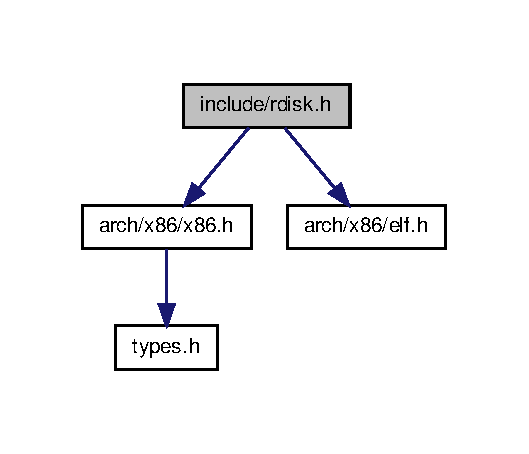
\includegraphics[width=254pt]{rdisk_8h__incl}
\end{center}
\end{figure}
\-This graph shows which files directly or indirectly include this file\-:\nopagebreak
\begin{figure}[H]
\begin{center}
\leavevmode
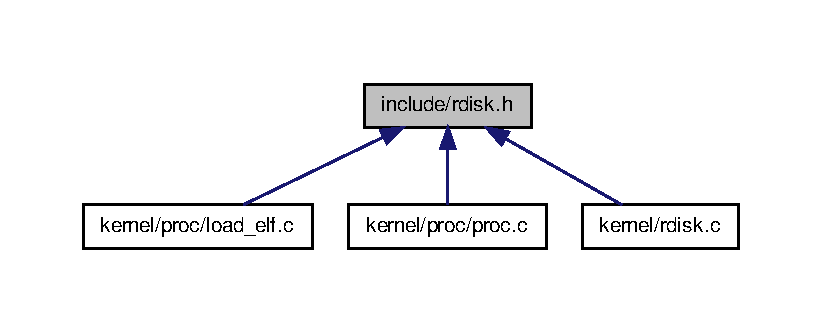
\includegraphics[width=350pt]{rdisk_8h__dep__incl}
\end{center}
\end{figure}
\subsection*{\-Defines}
\begin{DoxyCompactItemize}
\item 
\#define \hyperlink{rdisk_8h_af7ab12df78ebefa2212fca77338f56cd}{\-S\-E\-C\-T\-O\-R}~512
\item 
\#define \hyperlink{rdisk_8h_a173cb989ba031c300f459780e9b5f4da}{\-E\-L\-F\-\_\-\-M\-A\-G\-I\-C2}~0x8ec031fc
\end{DoxyCompactItemize}
\subsection*{\-Functions}
\begin{DoxyCompactItemize}
\item 
void \hyperlink{rdisk_8h_a8bc2062a175b7c74607a2498ac997657}{readsect} (void $\ast$, \hyperlink{types_8h_a435d1572bf3f880d55459d9805097f62}{uint32\-\_\-t})
\item 
void \hyperlink{rdisk_8h_a687601dc22e8d4d8407608c91fd325eb}{readseg} (\hyperlink{types_8h_a435d1572bf3f880d55459d9805097f62}{uint32\-\_\-t}, \hyperlink{types_8h_a435d1572bf3f880d55459d9805097f62}{uint32\-\_\-t}, \hyperlink{types_8h_a435d1572bf3f880d55459d9805097f62}{uint32\-\_\-t})
\item 
void \hyperlink{rdisk_8h_a63222d4a07c38c198de5bd116a001935}{waitdisk} (void)
\end{DoxyCompactItemize}


\subsection{\-Define \-Documentation}
\hypertarget{rdisk_8h_a173cb989ba031c300f459780e9b5f4da}{\index{rdisk.\-h@{rdisk.\-h}!\-E\-L\-F\-\_\-\-M\-A\-G\-I\-C2@{\-E\-L\-F\-\_\-\-M\-A\-G\-I\-C2}}
\index{\-E\-L\-F\-\_\-\-M\-A\-G\-I\-C2@{\-E\-L\-F\-\_\-\-M\-A\-G\-I\-C2}!rdisk.h@{rdisk.\-h}}
\subsubsection[{\-E\-L\-F\-\_\-\-M\-A\-G\-I\-C2}]{\setlength{\rightskip}{0pt plus 5cm}\#define {\bf \-E\-L\-F\-\_\-\-M\-A\-G\-I\-C2}~0x8ec031fc}}\label{rdisk_8h_a173cb989ba031c300f459780e9b5f4da}


\-Definition at line 9 of file rdisk.\-h.

\hypertarget{rdisk_8h_af7ab12df78ebefa2212fca77338f56cd}{\index{rdisk.\-h@{rdisk.\-h}!\-S\-E\-C\-T\-O\-R@{\-S\-E\-C\-T\-O\-R}}
\index{\-S\-E\-C\-T\-O\-R@{\-S\-E\-C\-T\-O\-R}!rdisk.h@{rdisk.\-h}}
\subsubsection[{\-S\-E\-C\-T\-O\-R}]{\setlength{\rightskip}{0pt plus 5cm}\#define {\bf \-S\-E\-C\-T\-O\-R}~512}}\label{rdisk_8h_af7ab12df78ebefa2212fca77338f56cd}


\-Definition at line 7 of file rdisk.\-h.



\subsection{\-Function \-Documentation}
\hypertarget{rdisk_8h_a8bc2062a175b7c74607a2498ac997657}{\index{rdisk.\-h@{rdisk.\-h}!readsect@{readsect}}
\index{readsect@{readsect}!rdisk.h@{rdisk.\-h}}
\subsubsection[{readsect}]{\setlength{\rightskip}{0pt plus 5cm}void {\bf readsect} (
\begin{DoxyParamCaption}
\item[{void $\ast$}]{, }
\item[{{\bf uint32\-\_\-t}}]{}
\end{DoxyParamCaption}
)}}\label{rdisk_8h_a8bc2062a175b7c74607a2498ac997657}


\-Definition at line 36 of file rdisk.\-c.

\hypertarget{rdisk_8h_a687601dc22e8d4d8407608c91fd325eb}{\index{rdisk.\-h@{rdisk.\-h}!readseg@{readseg}}
\index{readseg@{readseg}!rdisk.h@{rdisk.\-h}}
\subsubsection[{readseg}]{\setlength{\rightskip}{0pt plus 5cm}void {\bf readseg} (
\begin{DoxyParamCaption}
\item[{{\bf uint32\-\_\-t}}]{, }
\item[{{\bf uint32\-\_\-t}}]{, }
\item[{{\bf uint32\-\_\-t}}]{}
\end{DoxyParamCaption}
)}}\label{rdisk_8h_a687601dc22e8d4d8407608c91fd325eb}


\-Definition at line 11 of file rdisk.\-c.

\hypertarget{rdisk_8h_a63222d4a07c38c198de5bd116a001935}{\index{rdisk.\-h@{rdisk.\-h}!waitdisk@{waitdisk}}
\index{waitdisk@{waitdisk}!rdisk.h@{rdisk.\-h}}
\subsubsection[{waitdisk}]{\setlength{\rightskip}{0pt plus 5cm}void {\bf waitdisk} (
\begin{DoxyParamCaption}
\item[{void}]{}
\end{DoxyParamCaption}
)}}\label{rdisk_8h_a63222d4a07c38c198de5bd116a001935}


\-Definition at line 57 of file rdisk.\-c.


\hypertarget{stdarg_8h}{\section{include/stdarg.h \-File \-Reference}
\label{stdarg_8h}\index{include/stdarg.\-h@{include/stdarg.\-h}}
}
\-This graph shows which files directly or indirectly include this file\-:\nopagebreak
\begin{figure}[H]
\begin{center}
\leavevmode
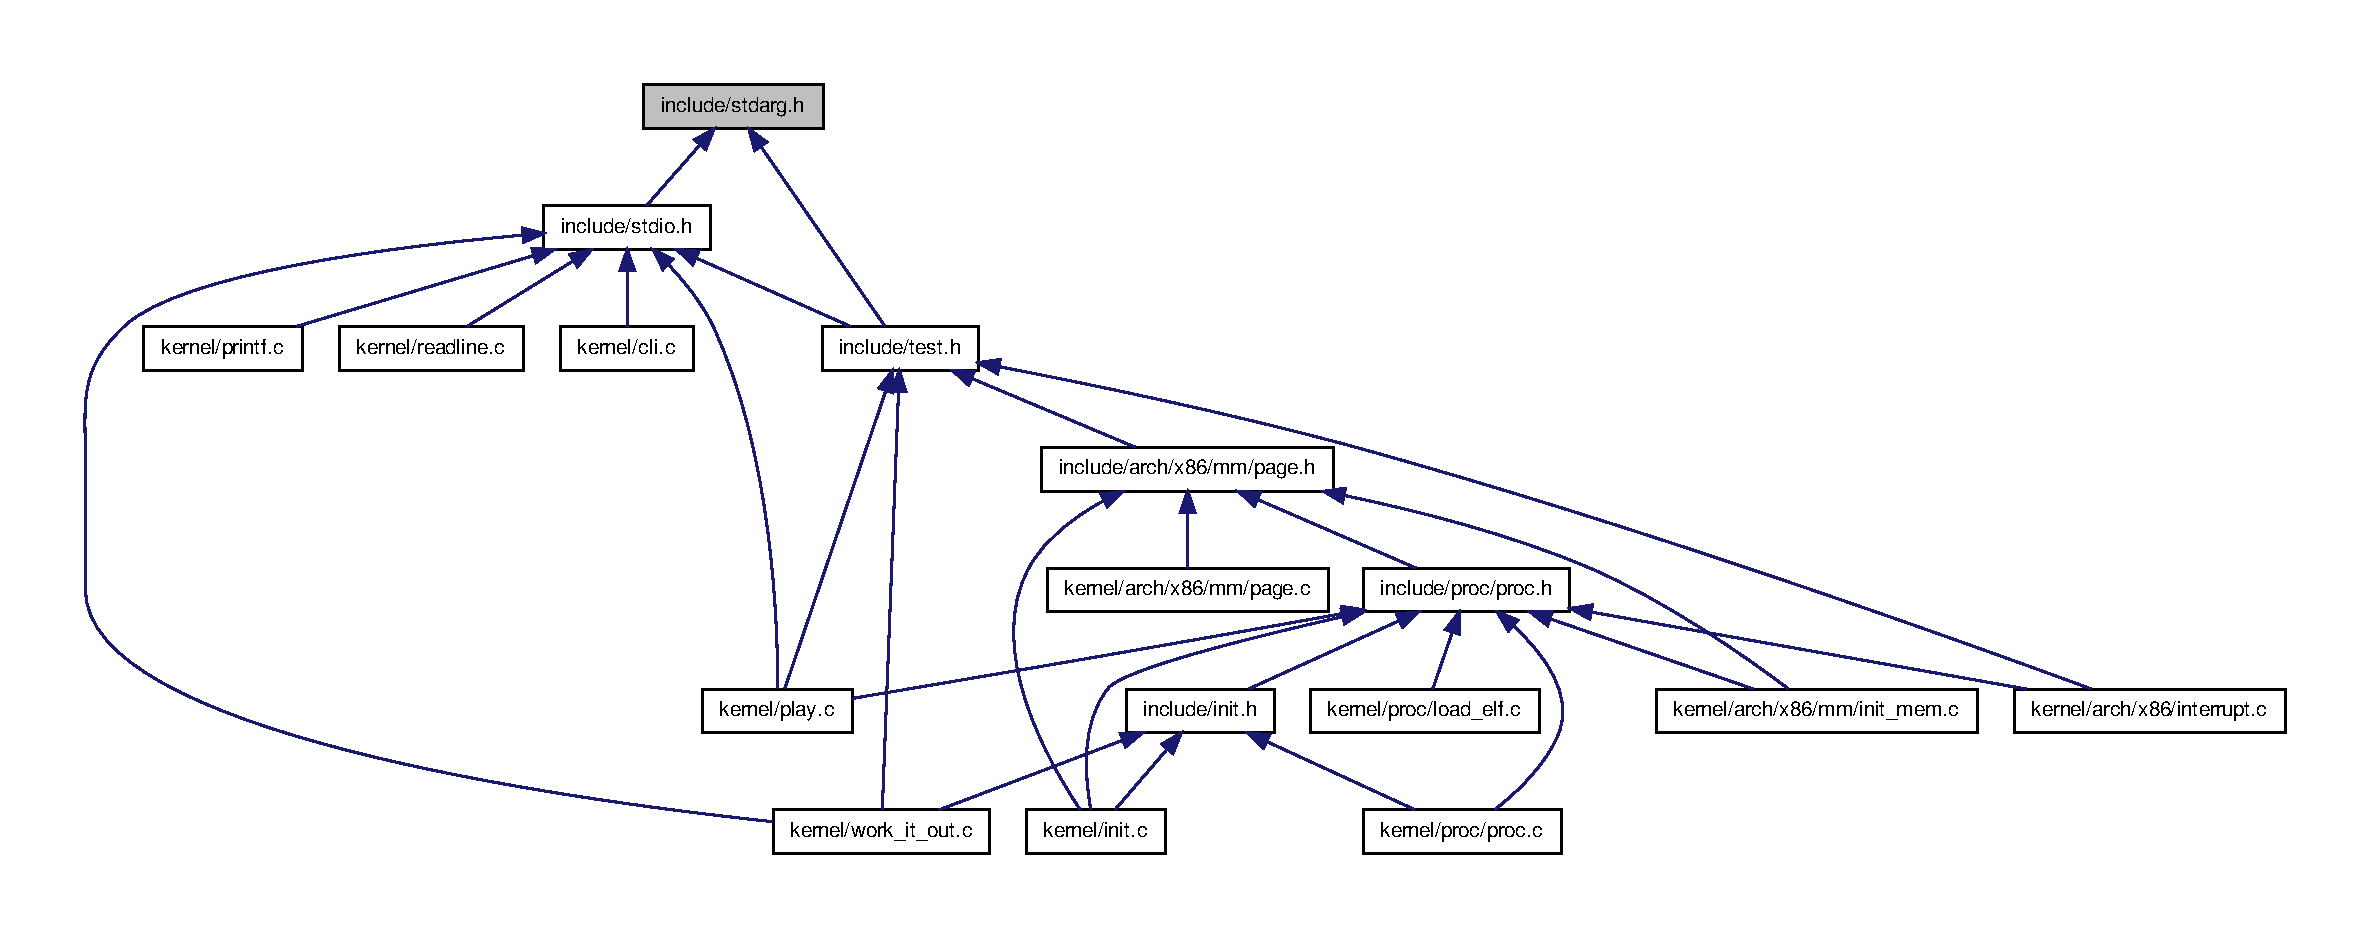
\includegraphics[width=350pt]{stdarg_8h__dep__incl}
\end{center}
\end{figure}
\subsection*{\-Defines}
\begin{DoxyCompactItemize}
\item 
\#define \hyperlink{stdarg_8h_aab7fc48f897f38522a7385eb78604907}{\-\_\-\-\_\-va\-\_\-size}(type)~(((sizeof(type) + sizeof(int)-\/1)/sizeof(int))$\ast$sizeof(int))
\item 
\#define \hyperlink{stdarg_8h_ade24ac546ea93fde2353ed2db8e89c66}{va\-\_\-start}(ap, last)~((ap) = (\hyperlink{stdarg_8h_abaefbc6cabb217bf0138d4f9c94d4775}{va\-\_\-list})\&(last) + \hyperlink{stdarg_8h_aab7fc48f897f38522a7385eb78604907}{\-\_\-\-\_\-va\-\_\-size}(last))
\item 
\#define \hyperlink{stdarg_8h_a81ebe6ea6253b0c6618e29de70fe10eb}{va\-\_\-arg}(ap, type)~($\ast$(type $\ast$)((ap) += \hyperlink{stdarg_8h_aab7fc48f897f38522a7385eb78604907}{\-\_\-\-\_\-va\-\_\-size}(type), (ap) -\/ \hyperlink{stdarg_8h_aab7fc48f897f38522a7385eb78604907}{\-\_\-\-\_\-va\-\_\-size}(type)))
\item 
\#define \hyperlink{stdarg_8h_acd9b3b9085ec072324c5fdac2b40304e}{va\-\_\-end}(ap)
\end{DoxyCompactItemize}
\subsection*{\-Typedefs}
\begin{DoxyCompactItemize}
\item 
typedef char $\ast$ \hyperlink{stdarg_8h_abaefbc6cabb217bf0138d4f9c94d4775}{va\-\_\-list}
\end{DoxyCompactItemize}


\subsection{\-Define \-Documentation}
\hypertarget{stdarg_8h_aab7fc48f897f38522a7385eb78604907}{\index{stdarg.\-h@{stdarg.\-h}!\-\_\-\-\_\-va\-\_\-size@{\-\_\-\-\_\-va\-\_\-size}}
\index{\-\_\-\-\_\-va\-\_\-size@{\-\_\-\-\_\-va\-\_\-size}!stdarg.h@{stdarg.\-h}}
\subsubsection[{\-\_\-\-\_\-va\-\_\-size}]{\setlength{\rightskip}{0pt plus 5cm}\#define {\bf \-\_\-\-\_\-va\-\_\-size}(
\begin{DoxyParamCaption}
\item[{}]{type}
\end{DoxyParamCaption}
)~(((sizeof(type) + sizeof(int)-\/1)/sizeof(int))$\ast$sizeof(int))}}\label{stdarg_8h_aab7fc48f897f38522a7385eb78604907}


\-Definition at line 11 of file stdarg.\-h.

\hypertarget{stdarg_8h_a81ebe6ea6253b0c6618e29de70fe10eb}{\index{stdarg.\-h@{stdarg.\-h}!va\-\_\-arg@{va\-\_\-arg}}
\index{va\-\_\-arg@{va\-\_\-arg}!stdarg.h@{stdarg.\-h}}
\subsubsection[{va\-\_\-arg}]{\setlength{\rightskip}{0pt plus 5cm}\#define {\bf va\-\_\-arg}(
\begin{DoxyParamCaption}
\item[{}]{ap, }
\item[{}]{type}
\end{DoxyParamCaption}
)~($\ast$(type $\ast$)((ap) += {\bf \-\_\-\-\_\-va\-\_\-size}(type), (ap) -\/ {\bf \-\_\-\-\_\-va\-\_\-size}(type)))}}\label{stdarg_8h_a81ebe6ea6253b0c6618e29de70fe10eb}


\-Definition at line 15 of file stdarg.\-h.

\hypertarget{stdarg_8h_acd9b3b9085ec072324c5fdac2b40304e}{\index{stdarg.\-h@{stdarg.\-h}!va\-\_\-end@{va\-\_\-end}}
\index{va\-\_\-end@{va\-\_\-end}!stdarg.h@{stdarg.\-h}}
\subsubsection[{va\-\_\-end}]{\setlength{\rightskip}{0pt plus 5cm}\#define {\bf va\-\_\-end}(
\begin{DoxyParamCaption}
\item[{}]{ap}
\end{DoxyParamCaption}
)}}\label{stdarg_8h_acd9b3b9085ec072324c5fdac2b40304e}


\-Definition at line 17 of file stdarg.\-h.

\hypertarget{stdarg_8h_ade24ac546ea93fde2353ed2db8e89c66}{\index{stdarg.\-h@{stdarg.\-h}!va\-\_\-start@{va\-\_\-start}}
\index{va\-\_\-start@{va\-\_\-start}!stdarg.h@{stdarg.\-h}}
\subsubsection[{va\-\_\-start}]{\setlength{\rightskip}{0pt plus 5cm}\#define {\bf va\-\_\-start}(
\begin{DoxyParamCaption}
\item[{}]{ap, }
\item[{}]{last}
\end{DoxyParamCaption}
)~((ap) = ({\bf va\-\_\-list})\&(last) + {\bf \-\_\-\-\_\-va\-\_\-size}(last))}}\label{stdarg_8h_ade24ac546ea93fde2353ed2db8e89c66}


\-Definition at line 13 of file stdarg.\-h.



\subsection{\-Typedef \-Documentation}
\hypertarget{stdarg_8h_abaefbc6cabb217bf0138d4f9c94d4775}{\index{stdarg.\-h@{stdarg.\-h}!va\-\_\-list@{va\-\_\-list}}
\index{va\-\_\-list@{va\-\_\-list}!stdarg.h@{stdarg.\-h}}
\subsubsection[{va\-\_\-list}]{\setlength{\rightskip}{0pt plus 5cm}typedef char$\ast$ {\bf va\-\_\-list}}}\label{stdarg_8h_abaefbc6cabb217bf0138d4f9c94d4775}
\-This code is a used in both linux and \-B\-S\-D 

\-Definition at line 9 of file stdarg.\-h.


\hypertarget{stdio_8h}{\section{include/stdio.h \-File \-Reference}
\label{stdio_8h}\index{include/stdio.\-h@{include/stdio.\-h}}
}
{\ttfamily \#include $<$stdarg.\-h$>$}\*
\-Include dependency graph for stdio.\-h\-:\nopagebreak
\begin{figure}[H]
\begin{center}
\leavevmode
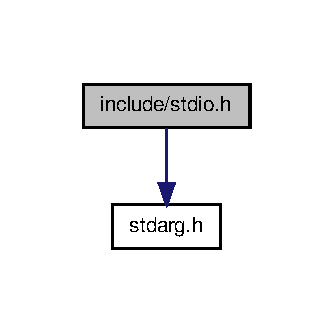
\includegraphics[width=160pt]{stdio_8h__incl}
\end{center}
\end{figure}
\-This graph shows which files directly or indirectly include this file\-:\nopagebreak
\begin{figure}[H]
\begin{center}
\leavevmode
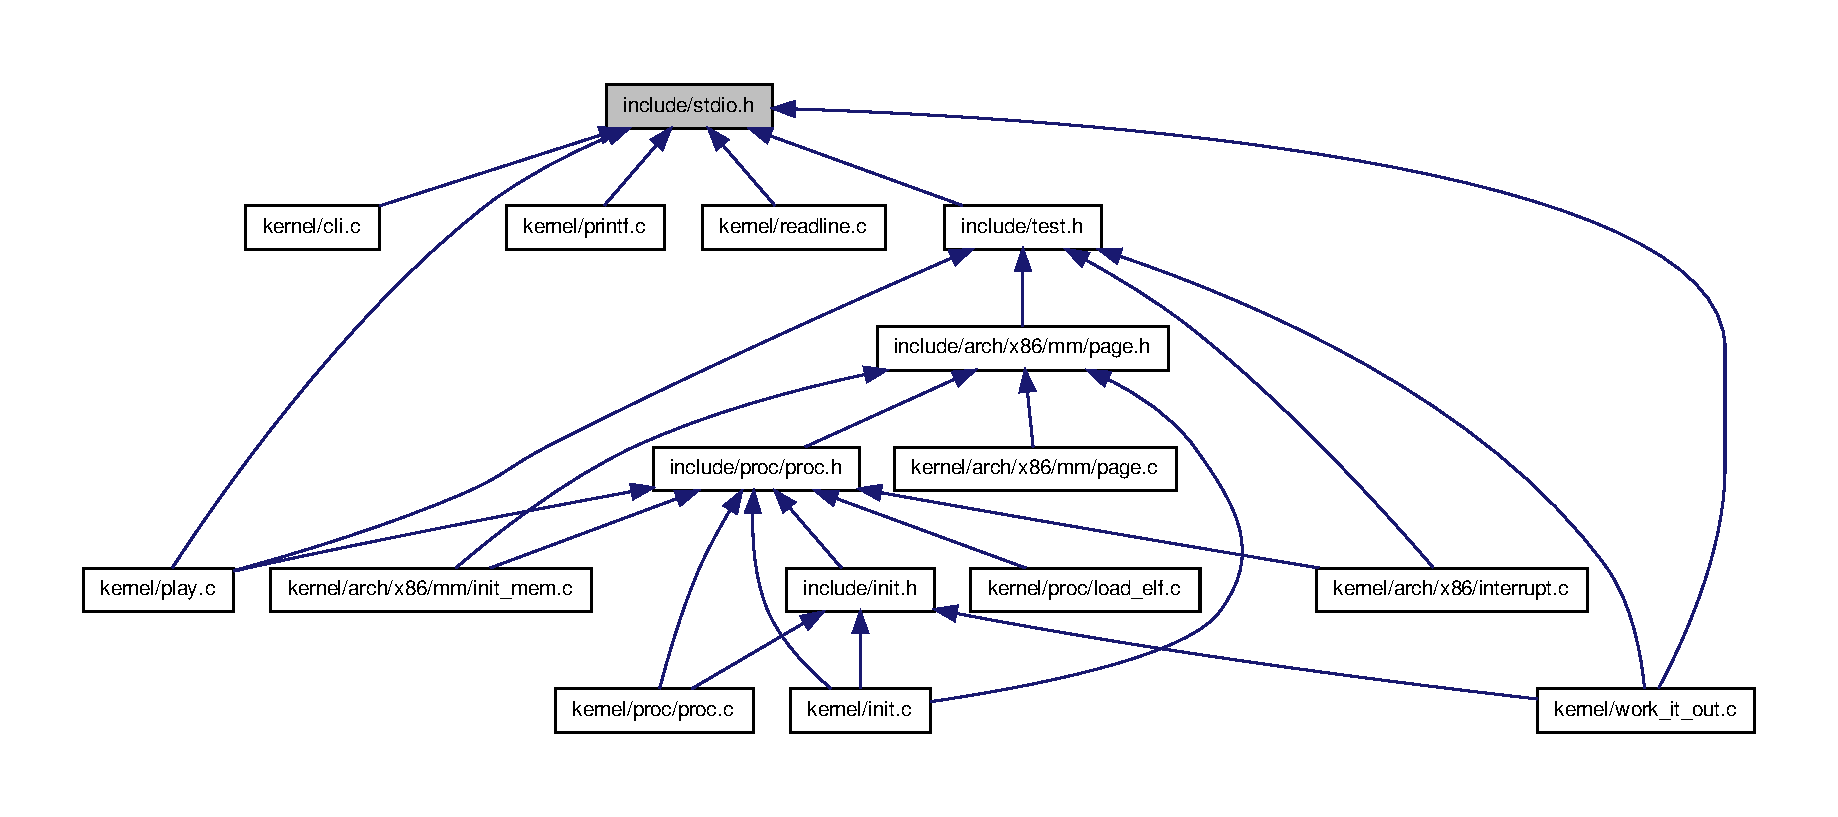
\includegraphics[width=350pt]{stdio_8h__dep__incl}
\end{center}
\end{figure}
\subsection*{\-Functions}
\begin{DoxyCompactItemize}
\item 
void \hyperlink{stdio_8h_a2d4bf280875c7c627a8548dcf7184187}{putchr} (int)
\item 
int \hyperlink{stdio_8h_a3e29caa20f7cffe18f410f01278905a8}{getchar} (void)
\item 
int \hyperlink{stdio_8h_a68c0540178fcff40a9b05dfa452900cf}{printk} (const char $\ast$,...)
\item 
int \hyperlink{stdio_8h_a9c91d3689b6c39cc51f8c8c6c63d920b}{vprintk} (const char $\ast$, \hyperlink{stdarg_8h_abaefbc6cabb217bf0138d4f9c94d4775}{va\-\_\-list})
\item 
int \hyperlink{stdio_8h_acbc64731fbdae6409954f586b33cd8aa}{kvprintk} (const char $\ast$, void($\ast$func)(int, int $\ast$), int $\ast$count, \hyperlink{stdarg_8h_abaefbc6cabb217bf0138d4f9c94d4775}{va\-\_\-list} ap)
\item 
void \hyperlink{stdio_8h_a4d96a0e0fd1a548e704a5408d77c33cb}{ksprintkn} (void($\ast$func)(int, int $\ast$), int $\ast$count, \hyperlink{types_8h_a2ba5f6c0633401558d277b2c0e4f758d}{uintmax\-\_\-t} num, int \hyperlink{memvals_8h_a0523cedff47e2441fc198b7770ec5d3f}{base}, int width, int padc)
\item 
char $\ast$ \hyperlink{stdio_8h_af3ce5d5d5bbaecd72030c27d331fb09e}{readline} (const char $\ast$)
\end{DoxyCompactItemize}


\subsection{\-Function \-Documentation}
\hypertarget{stdio_8h_a3e29caa20f7cffe18f410f01278905a8}{\index{stdio.\-h@{stdio.\-h}!getchar@{getchar}}
\index{getchar@{getchar}!stdio.h@{stdio.\-h}}
\subsubsection[{getchar}]{\setlength{\rightskip}{0pt plus 5cm}int {\bf getchar} (
\begin{DoxyParamCaption}
\item[{void}]{}
\end{DoxyParamCaption}
)}}\label{stdio_8h_a3e29caa20f7cffe18f410f01278905a8}


\-Definition at line 53 of file cli.\-c.

\hypertarget{stdio_8h_a4d96a0e0fd1a548e704a5408d77c33cb}{\index{stdio.\-h@{stdio.\-h}!ksprintkn@{ksprintkn}}
\index{ksprintkn@{ksprintkn}!stdio.h@{stdio.\-h}}
\subsubsection[{ksprintkn}]{\setlength{\rightskip}{0pt plus 5cm}void {\bf ksprintkn} (
\begin{DoxyParamCaption}
\item[{void($\ast$)(int, int $\ast$)}]{func, }
\item[{int $\ast$}]{count, }
\item[{{\bf uintmax\-\_\-t}}]{num, }
\item[{int}]{base, }
\item[{int}]{width, }
\item[{int}]{padc}
\end{DoxyParamCaption}
)}}\label{stdio_8h_a4d96a0e0fd1a548e704a5408d77c33cb}


\-Definition at line 10 of file printf.\-c.

\hypertarget{stdio_8h_acbc64731fbdae6409954f586b33cd8aa}{\index{stdio.\-h@{stdio.\-h}!kvprintk@{kvprintk}}
\index{kvprintk@{kvprintk}!stdio.h@{stdio.\-h}}
\subsubsection[{kvprintk}]{\setlength{\rightskip}{0pt plus 5cm}int {\bf kvprintk} (
\begin{DoxyParamCaption}
\item[{const char $\ast$}]{, }
\item[{void($\ast$)(int, int $\ast$)}]{func, }
\item[{int $\ast$}]{count, }
\item[{{\bf va\-\_\-list}}]{ap}
\end{DoxyParamCaption}
)}}\label{stdio_8h_acbc64731fbdae6409954f586b33cd8aa}


\-Definition at line 43 of file printf.\-c.

\hypertarget{stdio_8h_a68c0540178fcff40a9b05dfa452900cf}{\index{stdio.\-h@{stdio.\-h}!printk@{printk}}
\index{printk@{printk}!stdio.h@{stdio.\-h}}
\subsubsection[{printk}]{\setlength{\rightskip}{0pt plus 5cm}int {\bf printk} (
\begin{DoxyParamCaption}
\item[{const char $\ast$}]{, }
\item[{}]{...}
\end{DoxyParamCaption}
)}}\label{stdio_8h_a68c0540178fcff40a9b05dfa452900cf}


\-Definition at line 167 of file printf.\-c.

\hypertarget{stdio_8h_a2d4bf280875c7c627a8548dcf7184187}{\index{stdio.\-h@{stdio.\-h}!putchr@{putchr}}
\index{putchr@{putchr}!stdio.h@{stdio.\-h}}
\subsubsection[{putchr}]{\setlength{\rightskip}{0pt plus 5cm}void {\bf putchr} (
\begin{DoxyParamCaption}
\item[{int}]{}
\end{DoxyParamCaption}
)}}\label{stdio_8h_a2d4bf280875c7c627a8548dcf7184187}


\-Definition at line 49 of file cli.\-c.

\hypertarget{stdio_8h_af3ce5d5d5bbaecd72030c27d331fb09e}{\index{stdio.\-h@{stdio.\-h}!readline@{readline}}
\index{readline@{readline}!stdio.h@{stdio.\-h}}
\subsubsection[{readline}]{\setlength{\rightskip}{0pt plus 5cm}char$\ast$ {\bf readline} (
\begin{DoxyParamCaption}
\item[{const char $\ast$}]{}
\end{DoxyParamCaption}
)}}\label{stdio_8h_af3ce5d5d5bbaecd72030c27d331fb09e}


\-Definition at line 10 of file readline.\-c.

\hypertarget{stdio_8h_a9c91d3689b6c39cc51f8c8c6c63d920b}{\index{stdio.\-h@{stdio.\-h}!vprintk@{vprintk}}
\index{vprintk@{vprintk}!stdio.h@{stdio.\-h}}
\subsubsection[{vprintk}]{\setlength{\rightskip}{0pt plus 5cm}int {\bf vprintk} (
\begin{DoxyParamCaption}
\item[{const char $\ast$}]{, }
\item[{{\bf va\-\_\-list}}]{}
\end{DoxyParamCaption}
)}}\label{stdio_8h_a9c91d3689b6c39cc51f8c8c6c63d920b}


\-Definition at line 160 of file printf.\-c.


\hypertarget{string_8h}{\section{include/string.h \-File \-Reference}
\label{string_8h}\index{include/string.\-h@{include/string.\-h}}
}
{\ttfamily \#include $<$types.\-h$>$}\*
\-Include dependency graph for string.\-h\-:\nopagebreak
\begin{figure}[H]
\begin{center}
\leavevmode
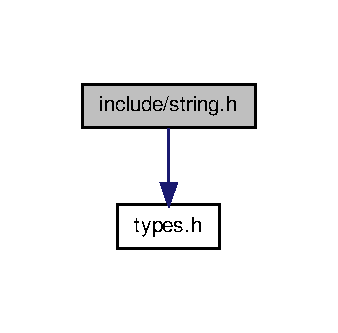
\includegraphics[width=162pt]{string_8h__incl}
\end{center}
\end{figure}
\-This graph shows which files directly or indirectly include this file\-:\nopagebreak
\begin{figure}[H]
\begin{center}
\leavevmode
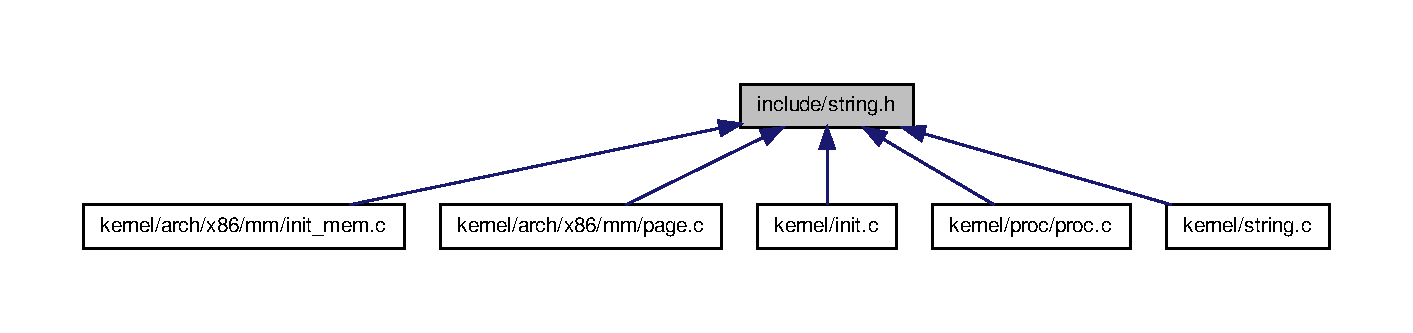
\includegraphics[width=350pt]{string_8h__dep__incl}
\end{center}
\end{figure}
\subsection*{\-Functions}
\begin{DoxyCompactItemize}
\item 
char $\ast$ \hyperlink{string_8h_ad684034d5a4f6552adda5cf41950b8d4}{strcpy} (char $\ast$dst, char $\ast$src)
\item 
char $\ast$ \hyperlink{string_8h_a6d39ca92e79fad11d3f7d3e5188e4d92}{strncpy} (char $\ast$dst, char $\ast$src, \hyperlink{types_8h_a435d1572bf3f880d55459d9805097f62}{uint32\-\_\-t} count)
\item 
char $\ast$ \hyperlink{string_8h_abdde96db1fac78cc35afc1e5028cf483}{strlcpy} (char $\ast$dst, char $\ast$src, \hyperlink{types_8h_a435d1572bf3f880d55459d9805097f62}{uint32\-\_\-t} count)
\item 
char $\ast$ \hyperlink{string_8h_a22e827f528ea79f9892aacd38b293bdf}{strcat} (char $\ast$dst, char $\ast$src)
\item 
char $\ast$ \hyperlink{string_8h_ae51600ca5b8e96a0be5adee1f8772f0e}{strncat} (char $\ast$dst, char $\ast$src, \hyperlink{types_8h_a435d1572bf3f880d55459d9805097f62}{uint32\-\_\-t} count)
\item 
char $\ast$ \hyperlink{string_8h_aa326a132cec03d769c0ff0f486a96de7}{strlcat} (char $\ast$dst, char $\ast$src, \hyperlink{types_8h_a435d1572bf3f880d55459d9805097f62}{uint32\-\_\-t} count)
\item 
int \hyperlink{string_8h_ae997a7b6c4609416ddcd95f838db5d75}{strcmp} (const char $\ast$cmp1, const char $\ast$cmp2)
\item 
int \hyperlink{string_8h_aa88a80a5cf672156253c790f939806e0}{strncmp} (const char $\ast$cmp1, const char $\ast$cmp2, \hyperlink{types_8h_a435d1572bf3f880d55459d9805097f62}{uint32\-\_\-t} count)
\item 
char $\ast$ \hyperlink{string_8h_afcd97f487174f9092b0f23c7ac78a55a}{strchr} (const char $\ast$str, int c)
\item 
char $\ast$ \hyperlink{string_8h_a9b5ffb90d9a30625617401e6a5999e85}{strrchr} (const char $\ast$str, int c)
\item 
char $\ast$ \hyperlink{string_8h_a7763ed4e32cb5fbefd0a01ab36a6e6f7}{strnchr} (const char $\ast$str, \hyperlink{types_8h_a435d1572bf3f880d55459d9805097f62}{uint32\-\_\-t} count, int c)
\item 
\hyperlink{types_8h_a435d1572bf3f880d55459d9805097f62}{uint32\-\_\-t} \hyperlink{string_8h_afa067738af4f322d2f39d719b170e2db}{strlen} (const char $\ast$str)
\item 
\hyperlink{types_8h_a435d1572bf3f880d55459d9805097f62}{uint32\-\_\-t} \hyperlink{string_8h_a2e7b2907250be8edc8e78f5dc91cd85b}{strnlen} (const char $\ast$str, \hyperlink{types_8h_a435d1572bf3f880d55459d9805097f62}{uint32\-\_\-t} count)
\item 
void $\ast$ \hyperlink{string_8h_a9e8681b3c39c9f02fb103b148f112e36}{memset} (void $\ast$dst, int c, \hyperlink{types_8h_a435d1572bf3f880d55459d9805097f62}{uint32\-\_\-t} count)
\item 
void $\ast$ \hyperlink{string_8h_a5beb6f763ff14a288fbe9c1f526579a3}{memcopy} (void $\ast$dst, const void $\ast$src, \hyperlink{types_8h_a435d1572bf3f880d55459d9805097f62}{uint32\-\_\-t} count)
\item 
void $\ast$ \hyperlink{string_8h_af6abef68f16ff453e6865153a3713ec1}{memmove} (void $\ast$dst, const void $\ast$src, \hyperlink{types_8h_a435d1572bf3f880d55459d9805097f62}{uint32\-\_\-t} count)
\item 
void $\ast$ \hyperlink{string_8h_a7bd42411a75cafc4dcde95c780316a8f}{memcmp} (const void $\ast$cmp1, const void $\ast$cmp2, \hyperlink{types_8h_a435d1572bf3f880d55459d9805097f62}{uint32\-\_\-t} count)
\end{DoxyCompactItemize}


\subsection{\-Function \-Documentation}
\hypertarget{string_8h_a7bd42411a75cafc4dcde95c780316a8f}{\index{string.\-h@{string.\-h}!memcmp@{memcmp}}
\index{memcmp@{memcmp}!string.h@{string.\-h}}
\subsubsection[{memcmp}]{\setlength{\rightskip}{0pt plus 5cm}void$\ast$ {\bf memcmp} (
\begin{DoxyParamCaption}
\item[{const void $\ast$}]{cmp1, }
\item[{const void $\ast$}]{cmp2, }
\item[{{\bf uint32\-\_\-t}}]{count}
\end{DoxyParamCaption}
)}}\label{string_8h_a7bd42411a75cafc4dcde95c780316a8f}
\hypertarget{string_8h_a5beb6f763ff14a288fbe9c1f526579a3}{\index{string.\-h@{string.\-h}!memcopy@{memcopy}}
\index{memcopy@{memcopy}!string.h@{string.\-h}}
\subsubsection[{memcopy}]{\setlength{\rightskip}{0pt plus 5cm}void$\ast$ {\bf memcopy} (
\begin{DoxyParamCaption}
\item[{void $\ast$}]{dst, }
\item[{const void $\ast$}]{src, }
\item[{{\bf uint32\-\_\-t}}]{count}
\end{DoxyParamCaption}
)}}\label{string_8h_a5beb6f763ff14a288fbe9c1f526579a3}


\-Definition at line 12 of file string.\-c.

\hypertarget{string_8h_af6abef68f16ff453e6865153a3713ec1}{\index{string.\-h@{string.\-h}!memmove@{memmove}}
\index{memmove@{memmove}!string.h@{string.\-h}}
\subsubsection[{memmove}]{\setlength{\rightskip}{0pt plus 5cm}void$\ast$ {\bf memmove} (
\begin{DoxyParamCaption}
\item[{void $\ast$}]{dst, }
\item[{const void $\ast$}]{src, }
\item[{{\bf uint32\-\_\-t}}]{count}
\end{DoxyParamCaption}
)}}\label{string_8h_af6abef68f16ff453e6865153a3713ec1}
\hypertarget{string_8h_a9e8681b3c39c9f02fb103b148f112e36}{\index{string.\-h@{string.\-h}!memset@{memset}}
\index{memset@{memset}!string.h@{string.\-h}}
\subsubsection[{memset}]{\setlength{\rightskip}{0pt plus 5cm}void$\ast$ {\bf memset} (
\begin{DoxyParamCaption}
\item[{void $\ast$}]{dst, }
\item[{int}]{c, }
\item[{{\bf uint32\-\_\-t}}]{count}
\end{DoxyParamCaption}
)}}\label{string_8h_a9e8681b3c39c9f02fb103b148f112e36}


\-Definition at line 24 of file string.\-c.

\hypertarget{string_8h_a22e827f528ea79f9892aacd38b293bdf}{\index{string.\-h@{string.\-h}!strcat@{strcat}}
\index{strcat@{strcat}!string.h@{string.\-h}}
\subsubsection[{strcat}]{\setlength{\rightskip}{0pt plus 5cm}char$\ast$ {\bf strcat} (
\begin{DoxyParamCaption}
\item[{char $\ast$}]{dst, }
\item[{char $\ast$}]{src}
\end{DoxyParamCaption}
)}}\label{string_8h_a22e827f528ea79f9892aacd38b293bdf}
\hypertarget{string_8h_afcd97f487174f9092b0f23c7ac78a55a}{\index{string.\-h@{string.\-h}!strchr@{strchr}}
\index{strchr@{strchr}!string.h@{string.\-h}}
\subsubsection[{strchr}]{\setlength{\rightskip}{0pt plus 5cm}char$\ast$ {\bf strchr} (
\begin{DoxyParamCaption}
\item[{const char $\ast$}]{str, }
\item[{int}]{c}
\end{DoxyParamCaption}
)}}\label{string_8h_afcd97f487174f9092b0f23c7ac78a55a}
\hypertarget{string_8h_ae997a7b6c4609416ddcd95f838db5d75}{\index{string.\-h@{string.\-h}!strcmp@{strcmp}}
\index{strcmp@{strcmp}!string.h@{string.\-h}}
\subsubsection[{strcmp}]{\setlength{\rightskip}{0pt plus 5cm}int {\bf strcmp} (
\begin{DoxyParamCaption}
\item[{const char $\ast$}]{cmp1, }
\item[{const char $\ast$}]{cmp2}
\end{DoxyParamCaption}
)}}\label{string_8h_ae997a7b6c4609416ddcd95f838db5d75}
\hypertarget{string_8h_ad684034d5a4f6552adda5cf41950b8d4}{\index{string.\-h@{string.\-h}!strcpy@{strcpy}}
\index{strcpy@{strcpy}!string.h@{string.\-h}}
\subsubsection[{strcpy}]{\setlength{\rightskip}{0pt plus 5cm}char$\ast$ {\bf strcpy} (
\begin{DoxyParamCaption}
\item[{char $\ast$}]{dst, }
\item[{char $\ast$}]{src}
\end{DoxyParamCaption}
)}}\label{string_8h_ad684034d5a4f6552adda5cf41950b8d4}
\hypertarget{string_8h_aa326a132cec03d769c0ff0f486a96de7}{\index{string.\-h@{string.\-h}!strlcat@{strlcat}}
\index{strlcat@{strlcat}!string.h@{string.\-h}}
\subsubsection[{strlcat}]{\setlength{\rightskip}{0pt plus 5cm}char$\ast$ {\bf strlcat} (
\begin{DoxyParamCaption}
\item[{char $\ast$}]{dst, }
\item[{char $\ast$}]{src, }
\item[{{\bf uint32\-\_\-t}}]{count}
\end{DoxyParamCaption}
)}}\label{string_8h_aa326a132cec03d769c0ff0f486a96de7}
\hypertarget{string_8h_abdde96db1fac78cc35afc1e5028cf483}{\index{string.\-h@{string.\-h}!strlcpy@{strlcpy}}
\index{strlcpy@{strlcpy}!string.h@{string.\-h}}
\subsubsection[{strlcpy}]{\setlength{\rightskip}{0pt plus 5cm}char$\ast$ {\bf strlcpy} (
\begin{DoxyParamCaption}
\item[{char $\ast$}]{dst, }
\item[{char $\ast$}]{src, }
\item[{{\bf uint32\-\_\-t}}]{count}
\end{DoxyParamCaption}
)}}\label{string_8h_abdde96db1fac78cc35afc1e5028cf483}
\hypertarget{string_8h_afa067738af4f322d2f39d719b170e2db}{\index{string.\-h@{string.\-h}!strlen@{strlen}}
\index{strlen@{strlen}!string.h@{string.\-h}}
\subsubsection[{strlen}]{\setlength{\rightskip}{0pt plus 5cm}{\bf uint32\-\_\-t} {\bf strlen} (
\begin{DoxyParamCaption}
\item[{const char $\ast$}]{str}
\end{DoxyParamCaption}
)}}\label{string_8h_afa067738af4f322d2f39d719b170e2db}
\hypertarget{string_8h_ae51600ca5b8e96a0be5adee1f8772f0e}{\index{string.\-h@{string.\-h}!strncat@{strncat}}
\index{strncat@{strncat}!string.h@{string.\-h}}
\subsubsection[{strncat}]{\setlength{\rightskip}{0pt plus 5cm}char$\ast$ {\bf strncat} (
\begin{DoxyParamCaption}
\item[{char $\ast$}]{dst, }
\item[{char $\ast$}]{src, }
\item[{{\bf uint32\-\_\-t}}]{count}
\end{DoxyParamCaption}
)}}\label{string_8h_ae51600ca5b8e96a0be5adee1f8772f0e}
\hypertarget{string_8h_a7763ed4e32cb5fbefd0a01ab36a6e6f7}{\index{string.\-h@{string.\-h}!strnchr@{strnchr}}
\index{strnchr@{strnchr}!string.h@{string.\-h}}
\subsubsection[{strnchr}]{\setlength{\rightskip}{0pt plus 5cm}char$\ast$ {\bf strnchr} (
\begin{DoxyParamCaption}
\item[{const char $\ast$}]{str, }
\item[{{\bf uint32\-\_\-t}}]{count, }
\item[{int}]{c}
\end{DoxyParamCaption}
)}}\label{string_8h_a7763ed4e32cb5fbefd0a01ab36a6e6f7}
\hypertarget{string_8h_aa88a80a5cf672156253c790f939806e0}{\index{string.\-h@{string.\-h}!strncmp@{strncmp}}
\index{strncmp@{strncmp}!string.h@{string.\-h}}
\subsubsection[{strncmp}]{\setlength{\rightskip}{0pt plus 5cm}int {\bf strncmp} (
\begin{DoxyParamCaption}
\item[{const char $\ast$}]{cmp1, }
\item[{const char $\ast$}]{cmp2, }
\item[{{\bf uint32\-\_\-t}}]{count}
\end{DoxyParamCaption}
)}}\label{string_8h_aa88a80a5cf672156253c790f939806e0}
\hypertarget{string_8h_a6d39ca92e79fad11d3f7d3e5188e4d92}{\index{string.\-h@{string.\-h}!strncpy@{strncpy}}
\index{strncpy@{strncpy}!string.h@{string.\-h}}
\subsubsection[{strncpy}]{\setlength{\rightskip}{0pt plus 5cm}char$\ast$ {\bf strncpy} (
\begin{DoxyParamCaption}
\item[{char $\ast$}]{dst, }
\item[{char $\ast$}]{src, }
\item[{{\bf uint32\-\_\-t}}]{count}
\end{DoxyParamCaption}
)}}\label{string_8h_a6d39ca92e79fad11d3f7d3e5188e4d92}
\hypertarget{string_8h_a2e7b2907250be8edc8e78f5dc91cd85b}{\index{string.\-h@{string.\-h}!strnlen@{strnlen}}
\index{strnlen@{strnlen}!string.h@{string.\-h}}
\subsubsection[{strnlen}]{\setlength{\rightskip}{0pt plus 5cm}{\bf uint32\-\_\-t} {\bf strnlen} (
\begin{DoxyParamCaption}
\item[{const char $\ast$}]{str, }
\item[{{\bf uint32\-\_\-t}}]{count}
\end{DoxyParamCaption}
)}}\label{string_8h_a2e7b2907250be8edc8e78f5dc91cd85b}


\-Definition at line 4 of file string.\-c.

\hypertarget{string_8h_a9b5ffb90d9a30625617401e6a5999e85}{\index{string.\-h@{string.\-h}!strrchr@{strrchr}}
\index{strrchr@{strrchr}!string.h@{string.\-h}}
\subsubsection[{strrchr}]{\setlength{\rightskip}{0pt plus 5cm}char$\ast$ {\bf strrchr} (
\begin{DoxyParamCaption}
\item[{const char $\ast$}]{str, }
\item[{int}]{c}
\end{DoxyParamCaption}
)}}\label{string_8h_a9b5ffb90d9a30625617401e6a5999e85}

\hypertarget{linkedlist_8h}{\section{include/structs/linkedlist.h \-File \-Reference}
\label{linkedlist_8h}\index{include/structs/linkedlist.\-h@{include/structs/linkedlist.\-h}}
}
\-This graph shows which files directly or indirectly include this file\-:\nopagebreak
\begin{figure}[H]
\begin{center}
\leavevmode
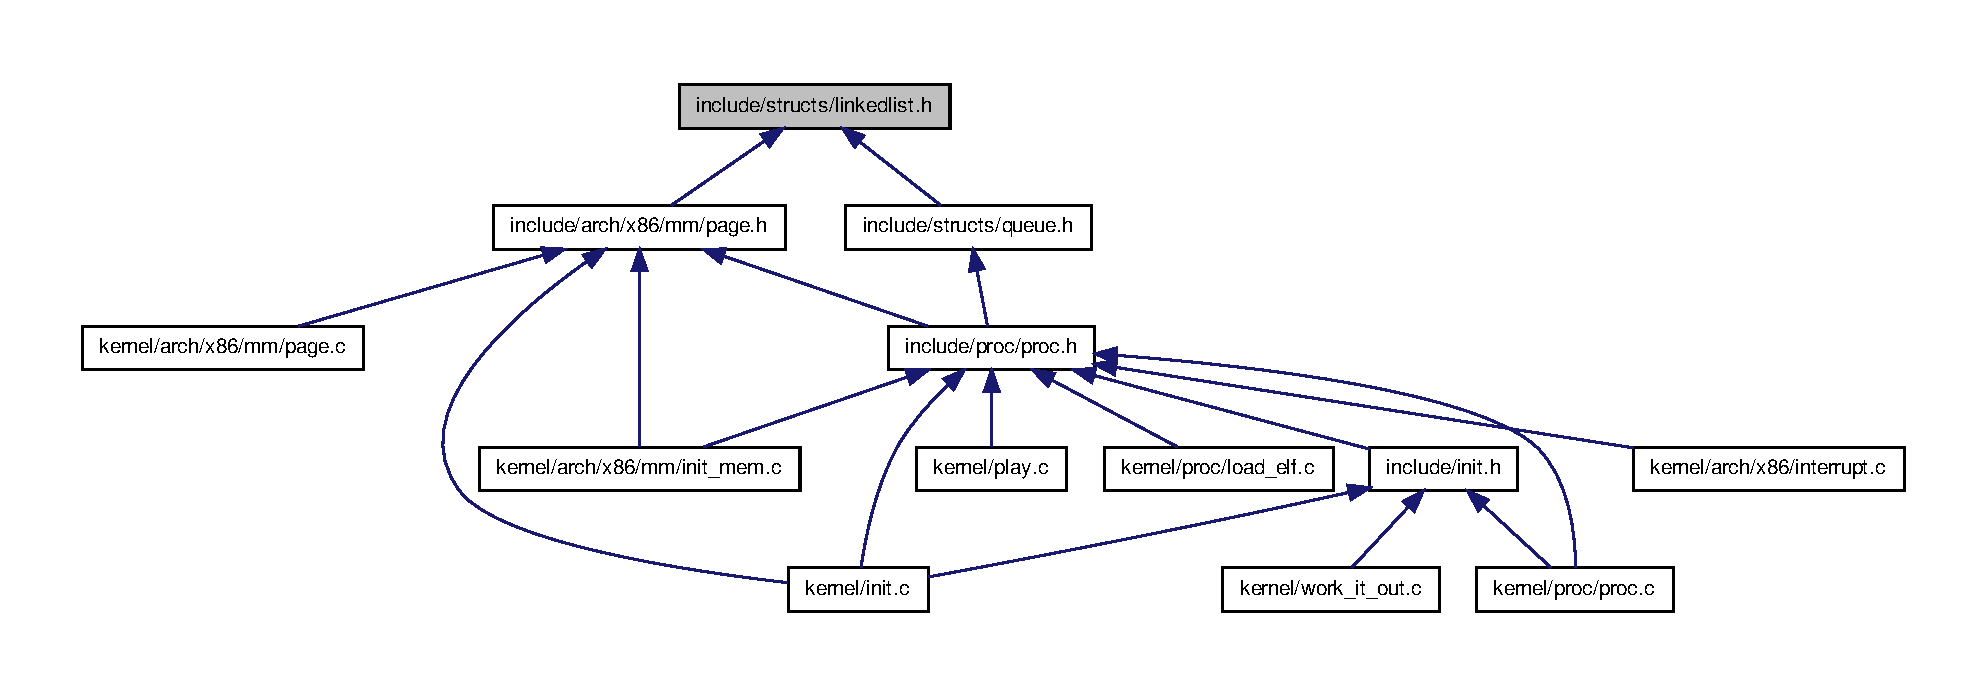
\includegraphics[width=350pt]{linkedlist_8h__dep__incl}
\end{center}
\end{figure}
\subsection*{\-Defines}
\begin{DoxyCompactItemize}
\item 
\#define \hyperlink{linkedlist_8h_a172799a84e7944bb109161db65bf99cf}{\-L\-I\-S\-T\-\_\-\-H\-E\-A\-D}(\-Instance, \-Type)
\item 
\#define \hyperlink{linkedlist_8h_ad9c04eb6522463f7d71aec6d81c7cb68}{\-L\-I\-S\-T\-\_\-\-H\-E\-A\-D\-\_\-\-I\-N\-I\-T}(head)~\{\hyperlink{types_8h_a070d2ce7b6bb7e5c05602aa8c308d0c4}{\-N\-U\-L\-L}\}
\item 
\#define \hyperlink{linkedlist_8h_aec2ccd0e8c215504508af23f04480be6}{\-L\-I\-S\-T\-\_\-\-E\-N\-T\-R\-Y}(type)
\item 
\#define \hyperlink{linkedlist_8h_a24a69fc0af564d2a576b06c194891c5a}{\-L\-I\-S\-T\-\_\-\-E\-M\-P\-T\-Y}(xhead)~((xhead)-\/$>$first == \hyperlink{types_8h_a070d2ce7b6bb7e5c05602aa8c308d0c4}{\-N\-U\-L\-L})
\item 
\#define \hyperlink{linkedlist_8h_a4beae2f37dbe52b21f754d987d3cec57}{\-L\-I\-S\-T\-\_\-\-F\-I\-R\-S\-T}(xhead)~((xhead)-\/$>$first)
\item 
\#define \hyperlink{linkedlist_8h_a6c28cf5a26558f950fd5632473390e36}{\-L\-I\-S\-T\-\_\-\-N\-E\-X\-T}(\hyperlink{structelement}{element}, field)~((\hyperlink{structelement}{element})-\/$>$field.\-next)
\item 
\#define \hyperlink{linkedlist_8h_ac1543beeb6d9224b60feb7a2703b2a87}{\-L\-I\-S\-T\-\_\-\-F\-O\-R\-E\-A\-C\-H}(var, head, field)
\item 
\#define \hyperlink{linkedlist_8h_a304b5b7f7bdcba2793eaba9c890991c3}{\-L\-I\-S\-T\-\_\-\-I\-N\-I\-T}(head)
\item 
\#define \hyperlink{linkedlist_8h_a3548dd269723b91fd13013cd8bd7d1c3}{\-L\-I\-S\-T\-\_\-\-I\-N\-S\-E\-R\-T\-\_\-\-A\-F\-T\-E\-R}(pre, \hyperlink{structelement}{element}, field)
\item 
\#define \hyperlink{linkedlist_8h_af7881d10124e52402743b6dfa4d445b0}{\-L\-I\-S\-T\-\_\-\-I\-N\-S\-E\-R\-T\-\_\-\-B\-E\-F\-O\-R\-E}(post, \hyperlink{structelement}{element}, field)
\item 
\#define \hyperlink{linkedlist_8h_a6c1914454bcfe361c908f1cc64e230f2}{\-L\-I\-S\-T\-\_\-\-R\-E\-M\-O\-V\-E}(\hyperlink{structelement}{element}, field)
\item 
\#define \hyperlink{linkedlist_8h_a4f07aefb8602b76649246d03eb570f03}{\-L\-I\-S\-T\-\_\-\-I\-N\-S\-E\-R\-T\-\_\-\-H\-E\-A\-D}(head, \hyperlink{structelement}{element}, field)
\end{DoxyCompactItemize}


\subsection{\-Define \-Documentation}
\hypertarget{linkedlist_8h_a24a69fc0af564d2a576b06c194891c5a}{\index{linkedlist.\-h@{linkedlist.\-h}!\-L\-I\-S\-T\-\_\-\-E\-M\-P\-T\-Y@{\-L\-I\-S\-T\-\_\-\-E\-M\-P\-T\-Y}}
\index{\-L\-I\-S\-T\-\_\-\-E\-M\-P\-T\-Y@{\-L\-I\-S\-T\-\_\-\-E\-M\-P\-T\-Y}!linkedlist.h@{linkedlist.\-h}}
\subsubsection[{\-L\-I\-S\-T\-\_\-\-E\-M\-P\-T\-Y}]{\setlength{\rightskip}{0pt plus 5cm}\#define {\bf \-L\-I\-S\-T\-\_\-\-E\-M\-P\-T\-Y}(
\begin{DoxyParamCaption}
\item[{}]{xhead}
\end{DoxyParamCaption}
)~((xhead)-\/$>$first == {\bf \-N\-U\-L\-L})}}\label{linkedlist_8h_a24a69fc0af564d2a576b06c194891c5a}
\-Functions of the list, first,next, insert, empty..etc 

\-Definition at line 36 of file linkedlist.\-h.

\hypertarget{linkedlist_8h_aec2ccd0e8c215504508af23f04480be6}{\index{linkedlist.\-h@{linkedlist.\-h}!\-L\-I\-S\-T\-\_\-\-E\-N\-T\-R\-Y@{\-L\-I\-S\-T\-\_\-\-E\-N\-T\-R\-Y}}
\index{\-L\-I\-S\-T\-\_\-\-E\-N\-T\-R\-Y@{\-L\-I\-S\-T\-\_\-\-E\-N\-T\-R\-Y}!linkedlist.h@{linkedlist.\-h}}
\subsubsection[{\-L\-I\-S\-T\-\_\-\-E\-N\-T\-R\-Y}]{\setlength{\rightskip}{0pt plus 5cm}\#define {\bf \-L\-I\-S\-T\-\_\-\-E\-N\-T\-R\-Y}(
\begin{DoxyParamCaption}
\item[{}]{type}
\end{DoxyParamCaption}
)}}\label{linkedlist_8h_aec2ccd0e8c215504508af23f04480be6}
{\bfseries \-Value\-:}
\begin{DoxyCode}
struct {\
                struct type *next;\
                struct type **prev;\
        }
\end{DoxyCode}


\-Definition at line 28 of file linkedlist.\-h.

\hypertarget{linkedlist_8h_a4beae2f37dbe52b21f754d987d3cec57}{\index{linkedlist.\-h@{linkedlist.\-h}!\-L\-I\-S\-T\-\_\-\-F\-I\-R\-S\-T@{\-L\-I\-S\-T\-\_\-\-F\-I\-R\-S\-T}}
\index{\-L\-I\-S\-T\-\_\-\-F\-I\-R\-S\-T@{\-L\-I\-S\-T\-\_\-\-F\-I\-R\-S\-T}!linkedlist.h@{linkedlist.\-h}}
\subsubsection[{\-L\-I\-S\-T\-\_\-\-F\-I\-R\-S\-T}]{\setlength{\rightskip}{0pt plus 5cm}\#define {\bf \-L\-I\-S\-T\-\_\-\-F\-I\-R\-S\-T}(
\begin{DoxyParamCaption}
\item[{}]{xhead}
\end{DoxyParamCaption}
)~((xhead)-\/$>$first)}}\label{linkedlist_8h_a4beae2f37dbe52b21f754d987d3cec57}


\-Definition at line 38 of file linkedlist.\-h.

\hypertarget{linkedlist_8h_ac1543beeb6d9224b60feb7a2703b2a87}{\index{linkedlist.\-h@{linkedlist.\-h}!\-L\-I\-S\-T\-\_\-\-F\-O\-R\-E\-A\-C\-H@{\-L\-I\-S\-T\-\_\-\-F\-O\-R\-E\-A\-C\-H}}
\index{\-L\-I\-S\-T\-\_\-\-F\-O\-R\-E\-A\-C\-H@{\-L\-I\-S\-T\-\_\-\-F\-O\-R\-E\-A\-C\-H}!linkedlist.h@{linkedlist.\-h}}
\subsubsection[{\-L\-I\-S\-T\-\_\-\-F\-O\-R\-E\-A\-C\-H}]{\setlength{\rightskip}{0pt plus 5cm}\#define {\bf \-L\-I\-S\-T\-\_\-\-F\-O\-R\-E\-A\-C\-H}(
\begin{DoxyParamCaption}
\item[{}]{var, }
\item[{}]{head, }
\item[{}]{field}
\end{DoxyParamCaption}
)}}\label{linkedlist_8h_ac1543beeb6d9224b60feb7a2703b2a87}
{\bfseries \-Value\-:}
\begin{DoxyCode}
for ((var) = LIST_FIRST((head));\
        (var);\
        (var) = LIST_NEXT((var),field))
\end{DoxyCode}
\-For each loop on teh list 

\-Definition at line 48 of file linkedlist.\-h.

\hypertarget{linkedlist_8h_a172799a84e7944bb109161db65bf99cf}{\index{linkedlist.\-h@{linkedlist.\-h}!\-L\-I\-S\-T\-\_\-\-H\-E\-A\-D@{\-L\-I\-S\-T\-\_\-\-H\-E\-A\-D}}
\index{\-L\-I\-S\-T\-\_\-\-H\-E\-A\-D@{\-L\-I\-S\-T\-\_\-\-H\-E\-A\-D}!linkedlist.h@{linkedlist.\-h}}
\subsubsection[{\-L\-I\-S\-T\-\_\-\-H\-E\-A\-D}]{\setlength{\rightskip}{0pt plus 5cm}\#define {\bf \-L\-I\-S\-T\-\_\-\-H\-E\-A\-D}(
\begin{DoxyParamCaption}
\item[{}]{\-Instance, }
\item[{}]{\-Type}
\end{DoxyParamCaption}
)}}\label{linkedlist_8h_a172799a84e7944bb109161db65bf99cf}
{\bfseries \-Value\-:}
\begin{DoxyCode}
struct Instance{\
                struct Type *first;\
        }
\end{DoxyCode}
a boot time list is a macro coded list to provide ability to make sequential lists at boot time. 

\-Definition at line 18 of file linkedlist.\-h.

\hypertarget{linkedlist_8h_ad9c04eb6522463f7d71aec6d81c7cb68}{\index{linkedlist.\-h@{linkedlist.\-h}!\-L\-I\-S\-T\-\_\-\-H\-E\-A\-D\-\_\-\-I\-N\-I\-T@{\-L\-I\-S\-T\-\_\-\-H\-E\-A\-D\-\_\-\-I\-N\-I\-T}}
\index{\-L\-I\-S\-T\-\_\-\-H\-E\-A\-D\-\_\-\-I\-N\-I\-T@{\-L\-I\-S\-T\-\_\-\-H\-E\-A\-D\-\_\-\-I\-N\-I\-T}!linkedlist.h@{linkedlist.\-h}}
\subsubsection[{\-L\-I\-S\-T\-\_\-\-H\-E\-A\-D\-\_\-\-I\-N\-I\-T}]{\setlength{\rightskip}{0pt plus 5cm}\#define {\bf \-L\-I\-S\-T\-\_\-\-H\-E\-A\-D\-\_\-\-I\-N\-I\-T}(
\begin{DoxyParamCaption}
\item[{}]{head}
\end{DoxyParamCaption}
)~\{{\bf \-N\-U\-L\-L}\}}}\label{linkedlist_8h_ad9c04eb6522463f7d71aec6d81c7cb68}


\-Definition at line 23 of file linkedlist.\-h.

\hypertarget{linkedlist_8h_a304b5b7f7bdcba2793eaba9c890991c3}{\index{linkedlist.\-h@{linkedlist.\-h}!\-L\-I\-S\-T\-\_\-\-I\-N\-I\-T@{\-L\-I\-S\-T\-\_\-\-I\-N\-I\-T}}
\index{\-L\-I\-S\-T\-\_\-\-I\-N\-I\-T@{\-L\-I\-S\-T\-\_\-\-I\-N\-I\-T}!linkedlist.h@{linkedlist.\-h}}
\subsubsection[{\-L\-I\-S\-T\-\_\-\-I\-N\-I\-T}]{\setlength{\rightskip}{0pt plus 5cm}\#define {\bf \-L\-I\-S\-T\-\_\-\-I\-N\-I\-T}(
\begin{DoxyParamCaption}
\item[{}]{head}
\end{DoxyParamCaption}
)}}\label{linkedlist_8h_a304b5b7f7bdcba2793eaba9c890991c3}
{\bfseries \-Value\-:}
\begin{DoxyCode}
do {\
                LIST_FIRST((head)) = NULL;\
        }while(0)
\end{DoxyCode}


\-Definition at line 55 of file linkedlist.\-h.

\hypertarget{linkedlist_8h_a3548dd269723b91fd13013cd8bd7d1c3}{\index{linkedlist.\-h@{linkedlist.\-h}!\-L\-I\-S\-T\-\_\-\-I\-N\-S\-E\-R\-T\-\_\-\-A\-F\-T\-E\-R@{\-L\-I\-S\-T\-\_\-\-I\-N\-S\-E\-R\-T\-\_\-\-A\-F\-T\-E\-R}}
\index{\-L\-I\-S\-T\-\_\-\-I\-N\-S\-E\-R\-T\-\_\-\-A\-F\-T\-E\-R@{\-L\-I\-S\-T\-\_\-\-I\-N\-S\-E\-R\-T\-\_\-\-A\-F\-T\-E\-R}!linkedlist.h@{linkedlist.\-h}}
\subsubsection[{\-L\-I\-S\-T\-\_\-\-I\-N\-S\-E\-R\-T\-\_\-\-A\-F\-T\-E\-R}]{\setlength{\rightskip}{0pt plus 5cm}\#define {\bf \-L\-I\-S\-T\-\_\-\-I\-N\-S\-E\-R\-T\-\_\-\-A\-F\-T\-E\-R}(
\begin{DoxyParamCaption}
\item[{}]{pre, }
\item[{}]{{\bf element}, }
\item[{}]{field}
\end{DoxyParamCaption}
)}}\label{linkedlist_8h_a3548dd269723b91fd13013cd8bd7d1c3}
{\bfseries \-Value\-:}
\begin{DoxyCode}
do{\
        if((LIST_NEXT((element),field) = (LIST_NEXT((pre),field))) != NULL)\
                LIST_NEXT(pre,field)->field.prev = &(LIST_NEXT((element),field)
      );\
        LIST_NEXT((pre),field)->field.next = (element);\
        (element)->field.prev = &(LIST_NEXT((pre),field));\
        } while(0)
\end{DoxyCode}


\-Definition at line 60 of file linkedlist.\-h.

\hypertarget{linkedlist_8h_af7881d10124e52402743b6dfa4d445b0}{\index{linkedlist.\-h@{linkedlist.\-h}!\-L\-I\-S\-T\-\_\-\-I\-N\-S\-E\-R\-T\-\_\-\-B\-E\-F\-O\-R\-E@{\-L\-I\-S\-T\-\_\-\-I\-N\-S\-E\-R\-T\-\_\-\-B\-E\-F\-O\-R\-E}}
\index{\-L\-I\-S\-T\-\_\-\-I\-N\-S\-E\-R\-T\-\_\-\-B\-E\-F\-O\-R\-E@{\-L\-I\-S\-T\-\_\-\-I\-N\-S\-E\-R\-T\-\_\-\-B\-E\-F\-O\-R\-E}!linkedlist.h@{linkedlist.\-h}}
\subsubsection[{\-L\-I\-S\-T\-\_\-\-I\-N\-S\-E\-R\-T\-\_\-\-B\-E\-F\-O\-R\-E}]{\setlength{\rightskip}{0pt plus 5cm}\#define {\bf \-L\-I\-S\-T\-\_\-\-I\-N\-S\-E\-R\-T\-\_\-\-B\-E\-F\-O\-R\-E}(
\begin{DoxyParamCaption}
\item[{}]{post, }
\item[{}]{{\bf element}, }
\item[{}]{field}
\end{DoxyParamCaption}
)}}\label{linkedlist_8h_af7881d10124e52402743b6dfa4d445b0}
{\bfseries \-Value\-:}
\begin{DoxyCode}
do{\
        (element)->field.prev = (post)->field.prev;\
        LIST_NEXT((element),field) = (post);\
        *(post)->field.prev = (element);\
        (post)->field.prev = &(LIST_NEXT((element),field));\
        } while(0)
\end{DoxyCode}


\-Definition at line 69 of file linkedlist.\-h.

\hypertarget{linkedlist_8h_a4f07aefb8602b76649246d03eb570f03}{\index{linkedlist.\-h@{linkedlist.\-h}!\-L\-I\-S\-T\-\_\-\-I\-N\-S\-E\-R\-T\-\_\-\-H\-E\-A\-D@{\-L\-I\-S\-T\-\_\-\-I\-N\-S\-E\-R\-T\-\_\-\-H\-E\-A\-D}}
\index{\-L\-I\-S\-T\-\_\-\-I\-N\-S\-E\-R\-T\-\_\-\-H\-E\-A\-D@{\-L\-I\-S\-T\-\_\-\-I\-N\-S\-E\-R\-T\-\_\-\-H\-E\-A\-D}!linkedlist.h@{linkedlist.\-h}}
\subsubsection[{\-L\-I\-S\-T\-\_\-\-I\-N\-S\-E\-R\-T\-\_\-\-H\-E\-A\-D}]{\setlength{\rightskip}{0pt plus 5cm}\#define {\bf \-L\-I\-S\-T\-\_\-\-I\-N\-S\-E\-R\-T\-\_\-\-H\-E\-A\-D}(
\begin{DoxyParamCaption}
\item[{}]{head, }
\item[{}]{{\bf element}, }
\item[{}]{field}
\end{DoxyParamCaption}
)}}\label{linkedlist_8h_a4f07aefb8602b76649246d03eb570f03}
{\bfseries \-Value\-:}
\begin{DoxyCode}
do {\
        if((LIST_NEXT((element), field) = LIST_FIRST((head))) != NULL)\
                LIST_FIRST((head))->field.prev = &(LIST_NEXT((element),field));
      \
        LIST_FIRST((head)) = (element);\
        (element)->field.prev = &(LIST_FIRST((head)));\
        } while(0)
\end{DoxyCode}


\-Definition at line 85 of file linkedlist.\-h.

\hypertarget{linkedlist_8h_a6c28cf5a26558f950fd5632473390e36}{\index{linkedlist.\-h@{linkedlist.\-h}!\-L\-I\-S\-T\-\_\-\-N\-E\-X\-T@{\-L\-I\-S\-T\-\_\-\-N\-E\-X\-T}}
\index{\-L\-I\-S\-T\-\_\-\-N\-E\-X\-T@{\-L\-I\-S\-T\-\_\-\-N\-E\-X\-T}!linkedlist.h@{linkedlist.\-h}}
\subsubsection[{\-L\-I\-S\-T\-\_\-\-N\-E\-X\-T}]{\setlength{\rightskip}{0pt plus 5cm}\#define {\bf \-L\-I\-S\-T\-\_\-\-N\-E\-X\-T}(
\begin{DoxyParamCaption}
\item[{}]{{\bf element}, }
\item[{}]{field}
\end{DoxyParamCaption}
)~(({\bf element})-\/$>$field.\-next)}}\label{linkedlist_8h_a6c28cf5a26558f950fd5632473390e36}


\-Definition at line 45 of file linkedlist.\-h.

\hypertarget{linkedlist_8h_a6c1914454bcfe361c908f1cc64e230f2}{\index{linkedlist.\-h@{linkedlist.\-h}!\-L\-I\-S\-T\-\_\-\-R\-E\-M\-O\-V\-E@{\-L\-I\-S\-T\-\_\-\-R\-E\-M\-O\-V\-E}}
\index{\-L\-I\-S\-T\-\_\-\-R\-E\-M\-O\-V\-E@{\-L\-I\-S\-T\-\_\-\-R\-E\-M\-O\-V\-E}!linkedlist.h@{linkedlist.\-h}}
\subsubsection[{\-L\-I\-S\-T\-\_\-\-R\-E\-M\-O\-V\-E}]{\setlength{\rightskip}{0pt plus 5cm}\#define {\bf \-L\-I\-S\-T\-\_\-\-R\-E\-M\-O\-V\-E}(
\begin{DoxyParamCaption}
\item[{}]{{\bf element}, }
\item[{}]{field}
\end{DoxyParamCaption}
)}}\label{linkedlist_8h_a6c1914454bcfe361c908f1cc64e230f2}
{\bfseries \-Value\-:}
\begin{DoxyCode}
do {\
        if(LIST_NEXT((element),field) != NULL)\
                LIST_NEXT((element),field)->field.prev =\
                        (element)->field.prev;\
        *(element)->field.prev = LIST_NEXT( (element), field);\
        }while(0)
\end{DoxyCode}


\-Definition at line 77 of file linkedlist.\-h.


\hypertarget{list_8h}{\section{include/structs/list.h \-File \-Reference}
\label{list_8h}\index{include/structs/list.\-h@{include/structs/list.\-h}}
}
\subsection*{\-Data \-Structures}
\begin{DoxyCompactItemize}
\item 
struct \hyperlink{structelement}{element}
\end{DoxyCompactItemize}

\hypertarget{queue_8h}{\section{include/structs/queue.h \-File \-Reference}
\label{queue_8h}\index{include/structs/queue.\-h@{include/structs/queue.\-h}}
}
{\ttfamily \#include $<$structs/linkedlist.\-h$>$}\*
\-Include dependency graph for queue.\-h\-:\nopagebreak
\begin{figure}[H]
\begin{center}
\leavevmode
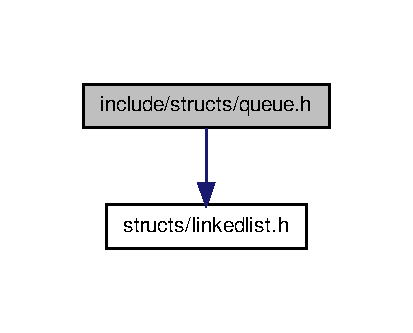
\includegraphics[width=198pt]{queue_8h__incl}
\end{center}
\end{figure}
\-This graph shows which files directly or indirectly include this file\-:\nopagebreak
\begin{figure}[H]
\begin{center}
\leavevmode
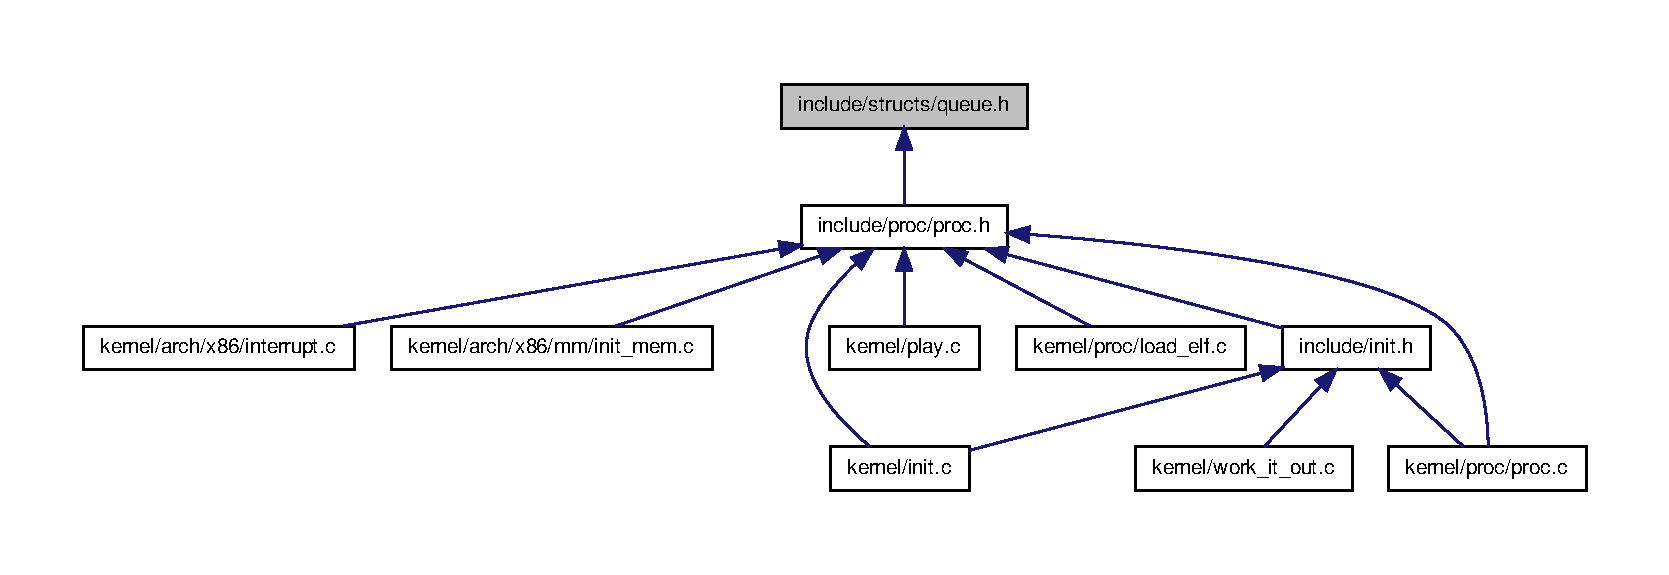
\includegraphics[width=350pt]{queue_8h__dep__incl}
\end{center}
\end{figure}
\subsection*{\-Defines}
\begin{DoxyCompactItemize}
\item 
\#define \hyperlink{queue_8h_a3c2acaeb30e70ab95dd72b823c2448b8}{\-L\-I\-F\-O\-\_\-\-H\-E\-A\-D}(name, member)
\item 
\#define \hyperlink{queue_8h_a2f5b3850b88c37f41361474a3dce33dd}{\-L\-I\-F\-O\-\_\-\-H\-E\-A\-D\-\_\-\-I\-N\-I\-T}(h)~\hyperlink{linkedlist_8h_a304b5b7f7bdcba2793eaba9c890991c3}{\-L\-I\-S\-T\-\_\-\-I\-N\-I\-T}(h)
\item 
\#define \hyperlink{queue_8h_aa64537311d4b0cfc059f31d5429f9b23}{\-L\-I\-F\-O\-\_\-\-E\-N\-T\-R\-Y}(entry)~\hyperlink{page_8h_af06dbf095a0a3cb262f4ee59b32c6c7b}{\-L\-I\-S\-T\-\_\-\-E\-N\-T\-R\-Y}(entry)
\item 
\#define \hyperlink{queue_8h_ac16b051d0de230bbbb909bd6b5ba707d}{\-L\-I\-F\-O\-\_\-\-F\-I\-R\-S\-T}(h)~((h)-\/$>$first)
\item 
\#define \hyperlink{queue_8h_abc74e2f948dd04a520ec87ad9ab6d61b}{\-L\-I\-F\-O\-\_\-\-I\-N\-I\-T}(h)~\hyperlink{queue_8h_ac16b051d0de230bbbb909bd6b5ba707d}{\-L\-I\-F\-O\-\_\-\-F\-I\-R\-S\-T}((h)) = \hyperlink{types_8h_a070d2ce7b6bb7e5c05602aa8c308d0c4}{\-N\-U\-L\-L}
\item 
\#define \hyperlink{queue_8h_a8fe9d8be9623b2270e928e4f3468166a}{\-L\-I\-F\-O\-\_\-\-P\-U\-S\-H}(h, \hyperlink{structelement}{element}, field)~\hyperlink{linkedlist_8h_a4f07aefb8602b76649246d03eb570f03}{\-L\-I\-S\-T\-\_\-\-I\-N\-S\-E\-R\-T\-\_\-\-H\-E\-A\-D}(h, \hyperlink{structelement}{element}, field)
\item 
\#define \hyperlink{queue_8h_ae4c49edec67ce10d1b179f171b70fb65}{\-L\-I\-F\-O\-\_\-\-P\-O\-P}(h, field)
\end{DoxyCompactItemize}


\subsection{\-Define \-Documentation}
\hypertarget{queue_8h_aa64537311d4b0cfc059f31d5429f9b23}{\index{queue.\-h@{queue.\-h}!\-L\-I\-F\-O\-\_\-\-E\-N\-T\-R\-Y@{\-L\-I\-F\-O\-\_\-\-E\-N\-T\-R\-Y}}
\index{\-L\-I\-F\-O\-\_\-\-E\-N\-T\-R\-Y@{\-L\-I\-F\-O\-\_\-\-E\-N\-T\-R\-Y}!queue.h@{queue.\-h}}
\subsubsection[{\-L\-I\-F\-O\-\_\-\-E\-N\-T\-R\-Y}]{\setlength{\rightskip}{0pt plus 5cm}\#define {\bf \-L\-I\-F\-O\-\_\-\-E\-N\-T\-R\-Y}(
\begin{DoxyParamCaption}
\item[{}]{entry}
\end{DoxyParamCaption}
)~{\bf \-L\-I\-S\-T\-\_\-\-E\-N\-T\-R\-Y}(entry)}}\label{queue_8h_aa64537311d4b0cfc059f31d5429f9b23}


\-Definition at line 20 of file queue.\-h.

\hypertarget{queue_8h_ac16b051d0de230bbbb909bd6b5ba707d}{\index{queue.\-h@{queue.\-h}!\-L\-I\-F\-O\-\_\-\-F\-I\-R\-S\-T@{\-L\-I\-F\-O\-\_\-\-F\-I\-R\-S\-T}}
\index{\-L\-I\-F\-O\-\_\-\-F\-I\-R\-S\-T@{\-L\-I\-F\-O\-\_\-\-F\-I\-R\-S\-T}!queue.h@{queue.\-h}}
\subsubsection[{\-L\-I\-F\-O\-\_\-\-F\-I\-R\-S\-T}]{\setlength{\rightskip}{0pt plus 5cm}\#define {\bf \-L\-I\-F\-O\-\_\-\-F\-I\-R\-S\-T}(
\begin{DoxyParamCaption}
\item[{}]{h}
\end{DoxyParamCaption}
)~((h)-\/$>$first)}}\label{queue_8h_ac16b051d0de230bbbb909bd6b5ba707d}


\-Definition at line 23 of file queue.\-h.

\hypertarget{queue_8h_a3c2acaeb30e70ab95dd72b823c2448b8}{\index{queue.\-h@{queue.\-h}!\-L\-I\-F\-O\-\_\-\-H\-E\-A\-D@{\-L\-I\-F\-O\-\_\-\-H\-E\-A\-D}}
\index{\-L\-I\-F\-O\-\_\-\-H\-E\-A\-D@{\-L\-I\-F\-O\-\_\-\-H\-E\-A\-D}!queue.h@{queue.\-h}}
\subsubsection[{\-L\-I\-F\-O\-\_\-\-H\-E\-A\-D}]{\setlength{\rightskip}{0pt plus 5cm}\#define {\bf \-L\-I\-F\-O\-\_\-\-H\-E\-A\-D}(
\begin{DoxyParamCaption}
\item[{}]{name, }
\item[{}]{member}
\end{DoxyParamCaption}
)}}\label{queue_8h_a3c2acaeb30e70ab95dd72b823c2448b8}
{\bfseries \-Value\-:}
\begin{DoxyCode}
struct name{            \
                struct member *first;   \
        }
\end{DoxyCode}


\-Definition at line 13 of file queue.\-h.

\hypertarget{queue_8h_a2f5b3850b88c37f41361474a3dce33dd}{\index{queue.\-h@{queue.\-h}!\-L\-I\-F\-O\-\_\-\-H\-E\-A\-D\-\_\-\-I\-N\-I\-T@{\-L\-I\-F\-O\-\_\-\-H\-E\-A\-D\-\_\-\-I\-N\-I\-T}}
\index{\-L\-I\-F\-O\-\_\-\-H\-E\-A\-D\-\_\-\-I\-N\-I\-T@{\-L\-I\-F\-O\-\_\-\-H\-E\-A\-D\-\_\-\-I\-N\-I\-T}!queue.h@{queue.\-h}}
\subsubsection[{\-L\-I\-F\-O\-\_\-\-H\-E\-A\-D\-\_\-\-I\-N\-I\-T}]{\setlength{\rightskip}{0pt plus 5cm}\#define {\bf \-L\-I\-F\-O\-\_\-\-H\-E\-A\-D\-\_\-\-I\-N\-I\-T}(
\begin{DoxyParamCaption}
\item[{}]{h}
\end{DoxyParamCaption}
)~{\bf \-L\-I\-S\-T\-\_\-\-I\-N\-I\-T}(h)}}\label{queue_8h_a2f5b3850b88c37f41361474a3dce33dd}


\-Definition at line 17 of file queue.\-h.

\hypertarget{queue_8h_abc74e2f948dd04a520ec87ad9ab6d61b}{\index{queue.\-h@{queue.\-h}!\-L\-I\-F\-O\-\_\-\-I\-N\-I\-T@{\-L\-I\-F\-O\-\_\-\-I\-N\-I\-T}}
\index{\-L\-I\-F\-O\-\_\-\-I\-N\-I\-T@{\-L\-I\-F\-O\-\_\-\-I\-N\-I\-T}!queue.h@{queue.\-h}}
\subsubsection[{\-L\-I\-F\-O\-\_\-\-I\-N\-I\-T}]{\setlength{\rightskip}{0pt plus 5cm}\#define {\bf \-L\-I\-F\-O\-\_\-\-I\-N\-I\-T}(
\begin{DoxyParamCaption}
\item[{}]{h}
\end{DoxyParamCaption}
)~{\bf \-L\-I\-F\-O\-\_\-\-F\-I\-R\-S\-T}((h)) = {\bf \-N\-U\-L\-L}}}\label{queue_8h_abc74e2f948dd04a520ec87ad9ab6d61b}


\-Definition at line 25 of file queue.\-h.

\hypertarget{queue_8h_ae4c49edec67ce10d1b179f171b70fb65}{\index{queue.\-h@{queue.\-h}!\-L\-I\-F\-O\-\_\-\-P\-O\-P@{\-L\-I\-F\-O\-\_\-\-P\-O\-P}}
\index{\-L\-I\-F\-O\-\_\-\-P\-O\-P@{\-L\-I\-F\-O\-\_\-\-P\-O\-P}!queue.h@{queue.\-h}}
\subsubsection[{\-L\-I\-F\-O\-\_\-\-P\-O\-P}]{\setlength{\rightskip}{0pt plus 5cm}\#define {\bf \-L\-I\-F\-O\-\_\-\-P\-O\-P}(
\begin{DoxyParamCaption}
\item[{}]{h, }
\item[{}]{field}
\end{DoxyParamCaption}
)}}\label{queue_8h_ae4c49edec67ce10d1b179f171b70fb65}
{\bfseries \-Value\-:}
\begin{DoxyCode}
LIST_FIRST((h));\
        LIST_REMOVE(LIST_FIRST((h)), field)
\end{DoxyCode}


\-Definition at line 31 of file queue.\-h.

\hypertarget{queue_8h_a8fe9d8be9623b2270e928e4f3468166a}{\index{queue.\-h@{queue.\-h}!\-L\-I\-F\-O\-\_\-\-P\-U\-S\-H@{\-L\-I\-F\-O\-\_\-\-P\-U\-S\-H}}
\index{\-L\-I\-F\-O\-\_\-\-P\-U\-S\-H@{\-L\-I\-F\-O\-\_\-\-P\-U\-S\-H}!queue.h@{queue.\-h}}
\subsubsection[{\-L\-I\-F\-O\-\_\-\-P\-U\-S\-H}]{\setlength{\rightskip}{0pt plus 5cm}\#define {\bf \-L\-I\-F\-O\-\_\-\-P\-U\-S\-H}(
\begin{DoxyParamCaption}
\item[{}]{h, }
\item[{}]{{\bf element}, }
\item[{}]{field}
\end{DoxyParamCaption}
)~{\bf \-L\-I\-S\-T\-\_\-\-I\-N\-S\-E\-R\-T\-\_\-\-H\-E\-A\-D}(h, {\bf element}, field)}}\label{queue_8h_a8fe9d8be9623b2270e928e4f3468166a}


\-Definition at line 28 of file queue.\-h.


\hypertarget{test_8h}{\section{include/test.h \-File \-Reference}
\label{test_8h}\index{include/test.\-h@{include/test.\-h}}
}
{\ttfamily \#include $<$stdio.\-h$>$}\*
{\ttfamily \#include $<$stdarg.\-h$>$}\*
\-Include dependency graph for test.\-h\-:\nopagebreak
\begin{figure}[H]
\begin{center}
\leavevmode
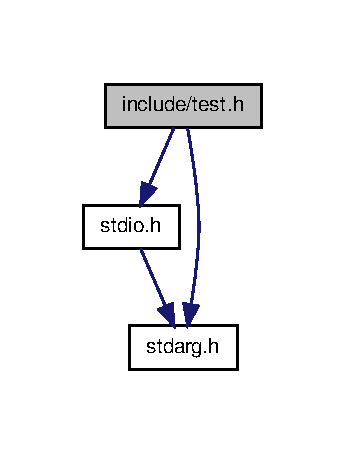
\includegraphics[width=165pt]{test_8h__incl}
\end{center}
\end{figure}
\-This graph shows which files directly or indirectly include this file\-:\nopagebreak
\begin{figure}[H]
\begin{center}
\leavevmode
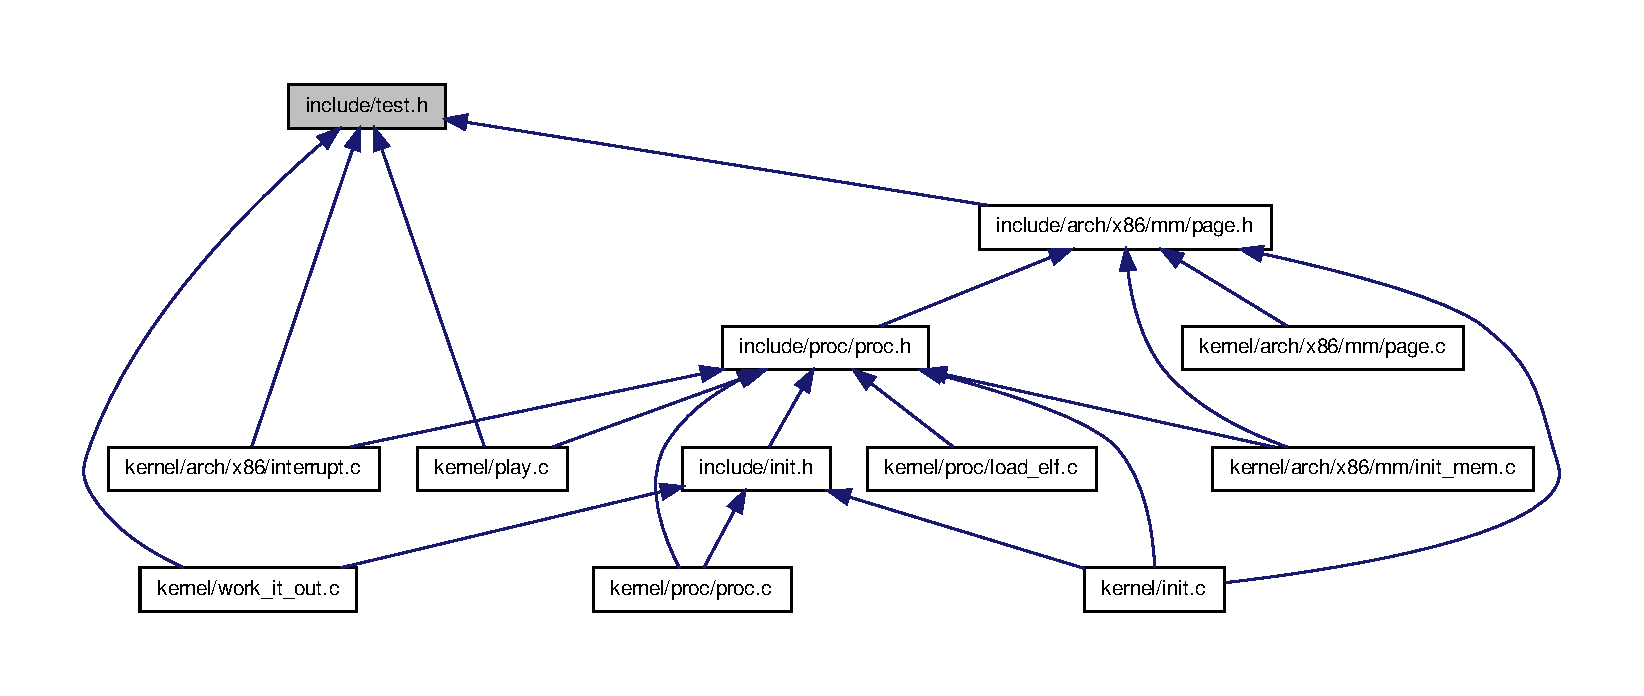
\includegraphics[width=350pt]{test_8h__dep__incl}
\end{center}
\end{figure}
\subsection*{\-Defines}
\begin{DoxyCompactItemize}
\item 
\#define \hyperlink{test_8h_a1445e207e36c97ff84c54b47288cea19}{panic}(...)
\item 
\#define \hyperlink{test_8h_af576bf8ffa22a44e53018c67095ffbf0}{assert}(x)
\end{DoxyCompactItemize}
\subsection*{\-Functions}
\begin{DoxyCompactItemize}
\item 
void \hyperlink{group__main_gaa3af12553c8338d80c22e90f5e12c1e1}{\-\_\-panic\-\_\-} (const char $\ast$, int, const char $\ast$,...) \hyperlink{struct____attribute____}{\-\_\-\-\_\-attribute\-\_\-\-\_\-}((noreturn))
\end{DoxyCompactItemize}


\subsection{\-Define \-Documentation}
\hypertarget{test_8h_af576bf8ffa22a44e53018c67095ffbf0}{\index{test.\-h@{test.\-h}!assert@{assert}}
\index{assert@{assert}!test.h@{test.\-h}}
\subsubsection[{assert}]{\setlength{\rightskip}{0pt plus 5cm}\#define {\bf assert}(
\begin{DoxyParamCaption}
\item[{}]{x}
\end{DoxyParamCaption}
)}}\label{test_8h_af576bf8ffa22a44e53018c67095ffbf0}
{\bfseries \-Value\-:}
\begin{DoxyCode}
if(!(x)){       \
                panic("Assertion Failed %s\n",#x);\
                }
\end{DoxyCode}


\-Definition at line 14 of file test.\-h.

\hypertarget{test_8h_a1445e207e36c97ff84c54b47288cea19}{\index{test.\-h@{test.\-h}!panic@{panic}}
\index{panic@{panic}!test.h@{test.\-h}}
\subsubsection[{panic}]{\setlength{\rightskip}{0pt plus 5cm}\#define {\bf panic}(
\begin{DoxyParamCaption}
\item[{}]{...}
\end{DoxyParamCaption}
)}}\label{test_8h_a1445e207e36c97ff84c54b47288cea19}
{\bfseries \-Value\-:}
\begin{DoxyCode}
printk(">>>>>> KERNEL PANIC <<<<<<<\n");\
        _panic_(__FILE__,__LINE__,__VA_ARGS__)
\end{DoxyCode}


\-Definition at line 10 of file test.\-h.


\hypertarget{types_8h}{\section{include/types.h \-File \-Reference}
\label{types_8h}\index{include/types.\-h@{include/types.\-h}}
}
\-This graph shows which files directly or indirectly include this file\-:\nopagebreak
\begin{figure}[H]
\begin{center}
\leavevmode
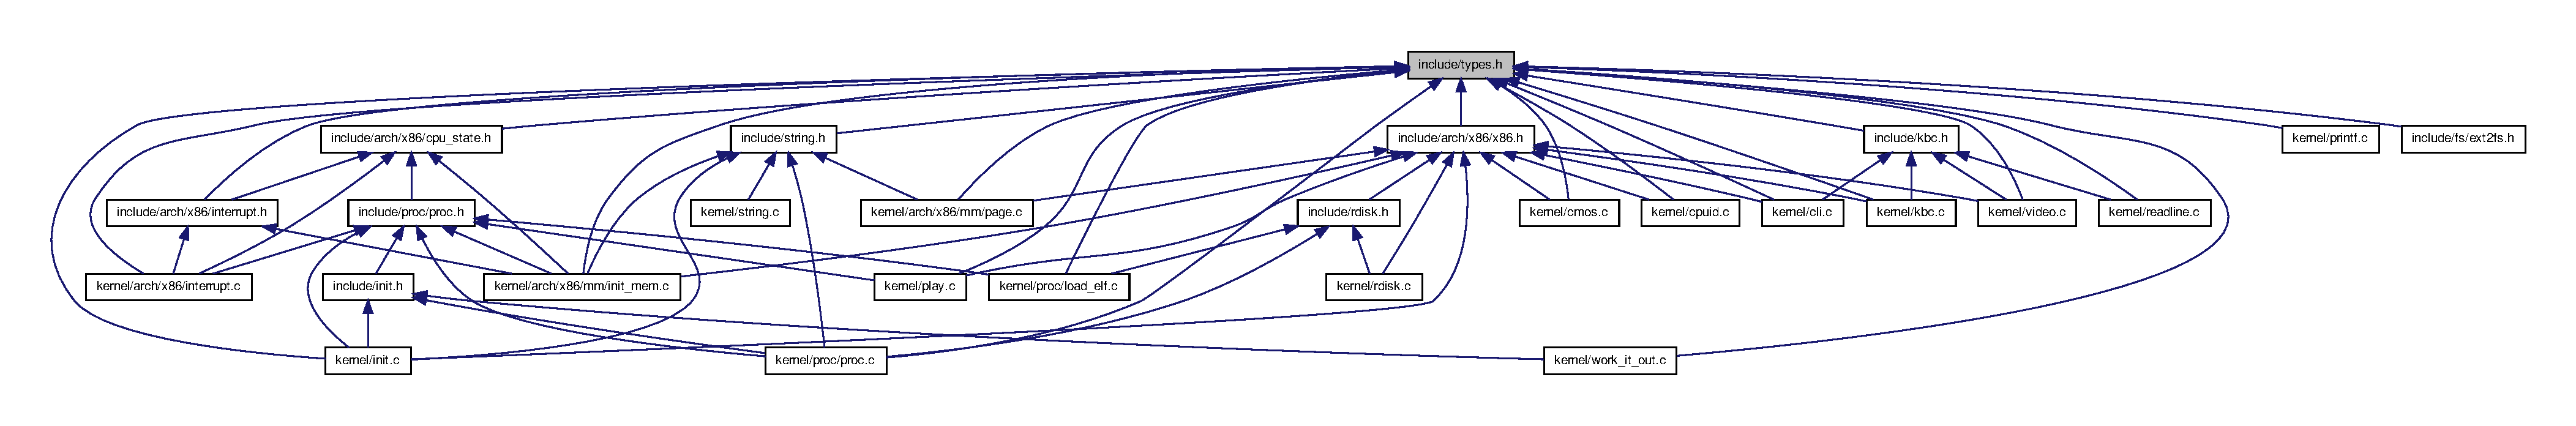
\includegraphics[width=350pt]{types_8h__dep__incl}
\end{center}
\end{figure}
\subsection*{\-Defines}
\begin{DoxyCompactItemize}
\item 
\#define \hyperlink{types_8h_a070d2ce7b6bb7e5c05602aa8c308d0c4}{\-N\-U\-L\-L}~((void$\ast$) 0)
\item 
\#define \hyperlink{types_8h_a2df9aa51d543ea63caff6ee2f2d2d4e4}{\-R\-O\-U\-N\-D\-\_\-\-D\-O\-W\-N}(x, y)
\item 
\#define \hyperlink{types_8h_a7a4ba4f2dbc3879306d8518c2670dd77}{\-R\-O\-U\-N\-D\-\_\-\-U\-P}(x, y)
\end{DoxyCompactItemize}
\subsection*{\-Typedefs}
\begin{DoxyCompactItemize}
\item 
typedef unsigned int \hyperlink{types_8h_a435d1572bf3f880d55459d9805097f62}{uint32\-\_\-t}
\item 
typedef unsigned short \hyperlink{types_8h_a273cf69d639a59973b6019625df33e30}{uint16\-\_\-t}
\item 
typedef unsigned char \hyperlink{types_8h_aba7bc1797add20fe3efdf37ced1182c5}{uint8\-\_\-t}
\item 
typedef unsigned long \hyperlink{types_8h_aa232ecf786a74ce5363c36c10798d2b1}{uint64\-\_\-t}
\item 
typedef char \hyperlink{types_8h_ad566f6541e98b74246db1a3a3a85ad49}{int8\-\_\-t}
\item 
typedef int \hyperlink{types_8h_a32f2e37ee053cf2ce8ca28d1f74630e5}{int32\-\_\-t}
\item 
typedef short \hyperlink{types_8h_aa343fa3b3d06292b959ffdd4c4703b06}{int16\-\_\-t}
\item 
typedef long long \hyperlink{types_8h_a996e72f71b11a5bb8b3b7b6936b1516d}{int64\-\_\-t}
\item 
typedef unsigned int \hyperlink{types_8h_a7c94ea6f8948649f8d181ae55911eeaf}{size\-\_\-t}
\item 
typedef \hyperlink{types_8h_aa232ecf786a74ce5363c36c10798d2b1}{uint64\-\_\-t} \hyperlink{types_8h_a2ba5f6c0633401558d277b2c0e4f758d}{uintmax\-\_\-t}
\item 
typedef \hyperlink{types_8h_a996e72f71b11a5bb8b3b7b6936b1516d}{int64\-\_\-t} \hyperlink{types_8h_a036cd61bb4b30bb510b9538af4cebd1d}{intmax\-\_\-t}
\item 
typedef \hyperlink{types_8h_a435d1572bf3f880d55459d9805097f62}{uint32\-\_\-t} \hyperlink{types_8h_a089269ab3c13f602c75d4c7820175d67}{reg\-\_\-t}
\item 
typedef \hyperlink{types_8h_a435d1572bf3f880d55459d9805097f62}{uint32\-\_\-t} \hyperlink{types_8h_a9f047c1f0917f6184a7a013d4b4277a6}{paddr\-\_\-t}
\item 
typedef \hyperlink{types_8h_a435d1572bf3f880d55459d9805097f62}{uint32\-\_\-t} \hyperlink{types_8h_a53428b953a0ae6fba02a5b3596c867e0}{vaddr\-\_\-t}
\end{DoxyCompactItemize}


\subsection{\-Define \-Documentation}
\hypertarget{types_8h_a070d2ce7b6bb7e5c05602aa8c308d0c4}{\index{types.\-h@{types.\-h}!\-N\-U\-L\-L@{\-N\-U\-L\-L}}
\index{\-N\-U\-L\-L@{\-N\-U\-L\-L}!types.h@{types.\-h}}
\subsubsection[{\-N\-U\-L\-L}]{\setlength{\rightskip}{0pt plus 5cm}\#define {\bf \-N\-U\-L\-L}~((void$\ast$) 0)}}\label{types_8h_a070d2ce7b6bb7e5c05602aa8c308d0c4}


\-Definition at line 8 of file types.\-h.

\hypertarget{types_8h_a2df9aa51d543ea63caff6ee2f2d2d4e4}{\index{types.\-h@{types.\-h}!\-R\-O\-U\-N\-D\-\_\-\-D\-O\-W\-N@{\-R\-O\-U\-N\-D\-\_\-\-D\-O\-W\-N}}
\index{\-R\-O\-U\-N\-D\-\_\-\-D\-O\-W\-N@{\-R\-O\-U\-N\-D\-\_\-\-D\-O\-W\-N}!types.h@{types.\-h}}
\subsubsection[{\-R\-O\-U\-N\-D\-\_\-\-D\-O\-W\-N}]{\setlength{\rightskip}{0pt plus 5cm}\#define {\bf \-R\-O\-U\-N\-D\-\_\-\-D\-O\-W\-N}(
\begin{DoxyParamCaption}
\item[{}]{x, }
\item[{}]{y}
\end{DoxyParamCaption}
)}}\label{types_8h_a2df9aa51d543ea63caff6ee2f2d2d4e4}
{\bfseries \-Value\-:}
\begin{DoxyCode}
({                                      \
        uint32_t z = (uint32_t)(x);     \
        (typeof(x)) (z - z % (y));      \
})
\end{DoxyCode}


\-Definition at line 27 of file types.\-h.

\hypertarget{types_8h_a7a4ba4f2dbc3879306d8518c2670dd77}{\index{types.\-h@{types.\-h}!\-R\-O\-U\-N\-D\-\_\-\-U\-P@{\-R\-O\-U\-N\-D\-\_\-\-U\-P}}
\index{\-R\-O\-U\-N\-D\-\_\-\-U\-P@{\-R\-O\-U\-N\-D\-\_\-\-U\-P}!types.h@{types.\-h}}
\subsubsection[{\-R\-O\-U\-N\-D\-\_\-\-U\-P}]{\setlength{\rightskip}{0pt plus 5cm}\#define {\bf \-R\-O\-U\-N\-D\-\_\-\-U\-P}(
\begin{DoxyParamCaption}
\item[{}]{x, }
\item[{}]{y}
\end{DoxyParamCaption}
)}}\label{types_8h_a7a4ba4f2dbc3879306d8518c2670dd77}
{\bfseries \-Value\-:}
\begin{DoxyCode}
({\
        uint32_t z = (uint32_t)(y);\
        (typeof(x)) (ROUND_DOWN(x,y) + y);\
})
\end{DoxyCode}


\-Definition at line 32 of file types.\-h.



\subsection{\-Typedef \-Documentation}
\hypertarget{types_8h_aa343fa3b3d06292b959ffdd4c4703b06}{\index{types.\-h@{types.\-h}!int16\-\_\-t@{int16\-\_\-t}}
\index{int16\-\_\-t@{int16\-\_\-t}!types.h@{types.\-h}}
\subsubsection[{int16\-\_\-t}]{\setlength{\rightskip}{0pt plus 5cm}typedef short {\bf int16\-\_\-t}}}\label{types_8h_aa343fa3b3d06292b959ffdd4c4703b06}


\-Definition at line 15 of file types.\-h.

\hypertarget{types_8h_a32f2e37ee053cf2ce8ca28d1f74630e5}{\index{types.\-h@{types.\-h}!int32\-\_\-t@{int32\-\_\-t}}
\index{int32\-\_\-t@{int32\-\_\-t}!types.h@{types.\-h}}
\subsubsection[{int32\-\_\-t}]{\setlength{\rightskip}{0pt plus 5cm}typedef int {\bf int32\-\_\-t}}}\label{types_8h_a32f2e37ee053cf2ce8ca28d1f74630e5}


\-Definition at line 14 of file types.\-h.

\hypertarget{types_8h_a996e72f71b11a5bb8b3b7b6936b1516d}{\index{types.\-h@{types.\-h}!int64\-\_\-t@{int64\-\_\-t}}
\index{int64\-\_\-t@{int64\-\_\-t}!types.h@{types.\-h}}
\subsubsection[{int64\-\_\-t}]{\setlength{\rightskip}{0pt plus 5cm}typedef long long {\bf int64\-\_\-t}}}\label{types_8h_a996e72f71b11a5bb8b3b7b6936b1516d}


\-Definition at line 16 of file types.\-h.

\hypertarget{types_8h_ad566f6541e98b74246db1a3a3a85ad49}{\index{types.\-h@{types.\-h}!int8\-\_\-t@{int8\-\_\-t}}
\index{int8\-\_\-t@{int8\-\_\-t}!types.h@{types.\-h}}
\subsubsection[{int8\-\_\-t}]{\setlength{\rightskip}{0pt plus 5cm}typedef char {\bf int8\-\_\-t}}}\label{types_8h_ad566f6541e98b74246db1a3a3a85ad49}


\-Definition at line 13 of file types.\-h.

\hypertarget{types_8h_a036cd61bb4b30bb510b9538af4cebd1d}{\index{types.\-h@{types.\-h}!intmax\-\_\-t@{intmax\-\_\-t}}
\index{intmax\-\_\-t@{intmax\-\_\-t}!types.h@{types.\-h}}
\subsubsection[{intmax\-\_\-t}]{\setlength{\rightskip}{0pt plus 5cm}typedef {\bf int64\-\_\-t} {\bf intmax\-\_\-t}}}\label{types_8h_a036cd61bb4b30bb510b9538af4cebd1d}


\-Definition at line 19 of file types.\-h.

\hypertarget{types_8h_a9f047c1f0917f6184a7a013d4b4277a6}{\index{types.\-h@{types.\-h}!paddr\-\_\-t@{paddr\-\_\-t}}
\index{paddr\-\_\-t@{paddr\-\_\-t}!types.h@{types.\-h}}
\subsubsection[{paddr\-\_\-t}]{\setlength{\rightskip}{0pt plus 5cm}typedef {\bf uint32\-\_\-t} {\bf paddr\-\_\-t}}}\label{types_8h_a9f047c1f0917f6184a7a013d4b4277a6}


\-Definition at line 23 of file types.\-h.

\hypertarget{types_8h_a089269ab3c13f602c75d4c7820175d67}{\index{types.\-h@{types.\-h}!reg\-\_\-t@{reg\-\_\-t}}
\index{reg\-\_\-t@{reg\-\_\-t}!types.h@{types.\-h}}
\subsubsection[{reg\-\_\-t}]{\setlength{\rightskip}{0pt plus 5cm}typedef {\bf uint32\-\_\-t} {\bf reg\-\_\-t}}}\label{types_8h_a089269ab3c13f602c75d4c7820175d67}


\-Definition at line 20 of file types.\-h.

\hypertarget{types_8h_a7c94ea6f8948649f8d181ae55911eeaf}{\index{types.\-h@{types.\-h}!size\-\_\-t@{size\-\_\-t}}
\index{size\-\_\-t@{size\-\_\-t}!types.h@{types.\-h}}
\subsubsection[{size\-\_\-t}]{\setlength{\rightskip}{0pt plus 5cm}typedef unsigned int {\bf size\-\_\-t}}}\label{types_8h_a7c94ea6f8948649f8d181ae55911eeaf}


\-Definition at line 17 of file types.\-h.

\hypertarget{types_8h_a273cf69d639a59973b6019625df33e30}{\index{types.\-h@{types.\-h}!uint16\-\_\-t@{uint16\-\_\-t}}
\index{uint16\-\_\-t@{uint16\-\_\-t}!types.h@{types.\-h}}
\subsubsection[{uint16\-\_\-t}]{\setlength{\rightskip}{0pt plus 5cm}typedef unsigned short {\bf uint16\-\_\-t}}}\label{types_8h_a273cf69d639a59973b6019625df33e30}


\-Definition at line 10 of file types.\-h.

\hypertarget{types_8h_a435d1572bf3f880d55459d9805097f62}{\index{types.\-h@{types.\-h}!uint32\-\_\-t@{uint32\-\_\-t}}
\index{uint32\-\_\-t@{uint32\-\_\-t}!types.h@{types.\-h}}
\subsubsection[{uint32\-\_\-t}]{\setlength{\rightskip}{0pt plus 5cm}typedef unsigned int {\bf uint32\-\_\-t}}}\label{types_8h_a435d1572bf3f880d55459d9805097f62}


\-Definition at line 9 of file types.\-h.

\hypertarget{types_8h_aa232ecf786a74ce5363c36c10798d2b1}{\index{types.\-h@{types.\-h}!uint64\-\_\-t@{uint64\-\_\-t}}
\index{uint64\-\_\-t@{uint64\-\_\-t}!types.h@{types.\-h}}
\subsubsection[{uint64\-\_\-t}]{\setlength{\rightskip}{0pt plus 5cm}typedef unsigned long {\bf uint64\-\_\-t}}}\label{types_8h_aa232ecf786a74ce5363c36c10798d2b1}


\-Definition at line 12 of file types.\-h.

\hypertarget{types_8h_aba7bc1797add20fe3efdf37ced1182c5}{\index{types.\-h@{types.\-h}!uint8\-\_\-t@{uint8\-\_\-t}}
\index{uint8\-\_\-t@{uint8\-\_\-t}!types.h@{types.\-h}}
\subsubsection[{uint8\-\_\-t}]{\setlength{\rightskip}{0pt plus 5cm}typedef unsigned char {\bf uint8\-\_\-t}}}\label{types_8h_aba7bc1797add20fe3efdf37ced1182c5}


\-Definition at line 11 of file types.\-h.

\hypertarget{types_8h_a2ba5f6c0633401558d277b2c0e4f758d}{\index{types.\-h@{types.\-h}!uintmax\-\_\-t@{uintmax\-\_\-t}}
\index{uintmax\-\_\-t@{uintmax\-\_\-t}!types.h@{types.\-h}}
\subsubsection[{uintmax\-\_\-t}]{\setlength{\rightskip}{0pt plus 5cm}typedef {\bf uint64\-\_\-t} {\bf uintmax\-\_\-t}}}\label{types_8h_a2ba5f6c0633401558d277b2c0e4f758d}


\-Definition at line 18 of file types.\-h.

\hypertarget{types_8h_a53428b953a0ae6fba02a5b3596c867e0}{\index{types.\-h@{types.\-h}!vaddr\-\_\-t@{vaddr\-\_\-t}}
\index{vaddr\-\_\-t@{vaddr\-\_\-t}!types.h@{types.\-h}}
\subsubsection[{vaddr\-\_\-t}]{\setlength{\rightskip}{0pt plus 5cm}typedef {\bf uint32\-\_\-t} {\bf vaddr\-\_\-t}}}\label{types_8h_a53428b953a0ae6fba02a5b3596c867e0}


\-Definition at line 24 of file types.\-h.


\hypertarget{video_8h}{\section{include/video.h \-File \-Reference}
\label{video_8h}\index{include/video.\-h@{include/video.\-h}}
}
\-This graph shows which files directly or indirectly include this file\-:\nopagebreak
\begin{figure}[H]
\begin{center}
\leavevmode
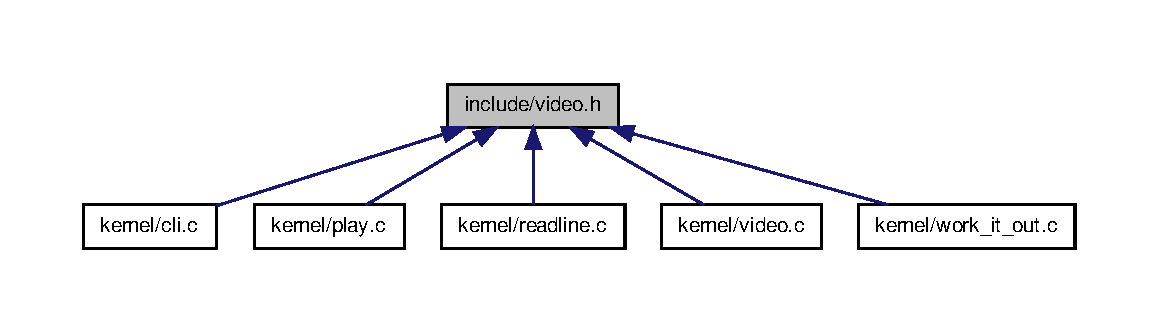
\includegraphics[width=350pt]{video_8h__dep__incl}
\end{center}
\end{figure}
\subsection*{\-Defines}
\begin{DoxyCompactItemize}
\item 
\#define \hyperlink{video_8h_af7656fc13f01cd69e72e98f2c25c53e0}{\-C\-G\-A\-\_\-\-I\-N\-D\-E\-X1}~0x3\-D4
\item 
\#define \hyperlink{video_8h_aca18d6ff81af020327872c0c44f22496}{\-C\-G\-A\-\_\-\-D\-A\-T\-A1}~0x3\-D5
\item 
\#define \hyperlink{video_8h_a997dc5abea4a2a3b1f5329661a40ee23}{\-C\-G\-A\-\_\-\-B\-U\-F\-F\-\_\-\-O\-F\-F}~0x\-B8000
\item 
\#define \hyperlink{video_8h_ad17fa086f20ce2f170d084c8d44e6aaa}{\-C\-G\-A\-\_\-\-C\-O\-L\-S}~80
\item 
\#define \hyperlink{video_8h_acccf116dbe23be4638439fdc3534b495}{\-C\-G\-A\-\_\-\-R\-O\-W\-S}~25
\item 
\#define \hyperlink{video_8h_a95147c043155dda6178fe12ba46c3a1d}{\-C\-G\-A\-\_\-\-S\-I\-Z\-E}~(\hyperlink{video_8h_acccf116dbe23be4638439fdc3534b495}{\-C\-G\-A\-\_\-\-R\-O\-W\-S} $\ast$ \hyperlink{video_8h_ad17fa086f20ce2f170d084c8d44e6aaa}{\-C\-G\-A\-\_\-\-C\-O\-L\-S})
\item 
\#define \hyperlink{video_8h_a2c546bb9d8660d44115f17f15d561fae}{\-C\-O\-L\-O\-R\-\_\-\-D\-A\-R\-K\-\_\-\-G\-R\-A\-Y}~0x0700
\item 
\#define \hyperlink{video_8h_a23c70d699a5a775bc2e1ebeb8603f630}{\-C\-O\-L\-O\-R\-\_\-\-B\-L\-U\-E}~0x0100
\item 
\#define \hyperlink{video_8h_afc9149f5de51bd9ac4f5ebbfa153f018}{\-C\-O\-L\-O\-R\-\_\-\-G\-R\-E\-E\-N}~0x0200
\item 
\#define \hyperlink{video_8h_ad86358bf19927183dd7b4ae215a29731}{\-C\-O\-L\-O\-R\-\_\-\-R\-E\-D}~0x0400
\item 
\#define \hyperlink{video_8h_a3aaf3b0287d26dfb6ecb3b1c46e950c8}{\-C\-O\-L\-O\-R\-\_\-\-G\-R\-A\-Y}~0x0800
\item 
\#define \hyperlink{video_8h_a9b44987ffdc2af19b635206b94334b69}{\-C\-O\-L\-O\-R\-\_\-\-W\-H\-I\-T\-E}~0x0f00
\item 
\#define \hyperlink{video_8h_ac7d5c1fe0c18a343fe1836c3ae808bda}{\-B\-A\-C\-K\-G\-R\-O\-U\-N\-D\-\_\-\-G\-R\-A\-Y}~0x7000
\item 
\#define \hyperlink{video_8h_ab433a51a42d2995552b67d262eee486b}{\-B\-A\-C\-K\-G\-R\-O\-U\-N\-D\-\_\-\-B\-L\-U\-E}~0x1000
\item 
\#define \hyperlink{video_8h_a53680f408ba52b07044ba502f15b717c}{\-B\-A\-C\-K\-G\-R\-O\-U\-N\-D\-\_\-\-G\-R\-E\-E\-N}~0x2000
\item 
\#define \hyperlink{video_8h_a9998726a5bcd3d57e125f0db5eebd5e3}{\-B\-A\-C\-K\-G\-R\-O\-U\-N\-D\-\_\-\-R\-E\-D}~0x4000
\item 
\#define \hyperlink{video_8h_a880dfb75bfdd4a9aa403cbc2a0b4002a}{\-B\-A\-C\-K\-G\-R\-O\-U\-N\-D\-\_\-\-B\-L\-I\-N\-K}~0x8000
\item 
\#define \hyperlink{video_8h_abfc3483dd6ef422df067ba52e258d50a}{\-B\-A\-C\-K\-G\-R\-O\-U\-N\-D\-\_\-\-W\-H\-I\-T\-E}~0x\-F000
\end{DoxyCompactItemize}
\subsection*{\-Functions}
\begin{DoxyCompactItemize}
\item 
void \hyperlink{video_8h_ab0ab5e709ff4fc4d57b7007cd4e305be}{cga\-\_\-init} (void)
\item 
\hyperlink{types_8h_a273cf69d639a59973b6019625df33e30}{uint16\-\_\-t} \hyperlink{video_8h_a395d60b7d3454851db53889826e8d72e}{cga\-\_\-get\-\_\-pos} (void)
\item 
void \hyperlink{video_8h_a7d6700bf85be86bf56d6be0dc1f2334c}{cga\-\_\-set\-\_\-pos} (\hyperlink{types_8h_a273cf69d639a59973b6019625df33e30}{uint16\-\_\-t})
\item 
void \hyperlink{video_8h_aca189a8fb5d14a6ccaabfb4ce606e20c}{cga\-\_\-putc} (int c)
\item 
void \hyperlink{video_8h_ae625a89575aec39216cedd42ea00fcac}{cga\-\_\-set\-\_\-attr} (\hyperlink{types_8h_a273cf69d639a59973b6019625df33e30}{uint16\-\_\-t})
\end{DoxyCompactItemize}
\subsection*{\-Variables}
\begin{DoxyCompactItemize}
\item 
\hyperlink{types_8h_a273cf69d639a59973b6019625df33e30}{uint16\-\_\-t} \hyperlink{video_8h_a58f3b0c1c71d999949fc2d085fa600ad}{cursor\-\_\-position}
\item 
\hyperlink{types_8h_a273cf69d639a59973b6019625df33e30}{uint16\-\_\-t} $\ast$ \hyperlink{video_8h_a628aae3cfe08b2d48d19b4d18b788e51}{char\-\_\-buff}
\end{DoxyCompactItemize}


\subsection{\-Define \-Documentation}
\hypertarget{video_8h_a880dfb75bfdd4a9aa403cbc2a0b4002a}{\index{video.\-h@{video.\-h}!\-B\-A\-C\-K\-G\-R\-O\-U\-N\-D\-\_\-\-B\-L\-I\-N\-K@{\-B\-A\-C\-K\-G\-R\-O\-U\-N\-D\-\_\-\-B\-L\-I\-N\-K}}
\index{\-B\-A\-C\-K\-G\-R\-O\-U\-N\-D\-\_\-\-B\-L\-I\-N\-K@{\-B\-A\-C\-K\-G\-R\-O\-U\-N\-D\-\_\-\-B\-L\-I\-N\-K}!video.h@{video.\-h}}
\subsubsection[{\-B\-A\-C\-K\-G\-R\-O\-U\-N\-D\-\_\-\-B\-L\-I\-N\-K}]{\setlength{\rightskip}{0pt plus 5cm}\#define {\bf \-B\-A\-C\-K\-G\-R\-O\-U\-N\-D\-\_\-\-B\-L\-I\-N\-K}~0x8000}}\label{video_8h_a880dfb75bfdd4a9aa403cbc2a0b4002a}


\-Definition at line 26 of file video.\-h.

\hypertarget{video_8h_ab433a51a42d2995552b67d262eee486b}{\index{video.\-h@{video.\-h}!\-B\-A\-C\-K\-G\-R\-O\-U\-N\-D\-\_\-\-B\-L\-U\-E@{\-B\-A\-C\-K\-G\-R\-O\-U\-N\-D\-\_\-\-B\-L\-U\-E}}
\index{\-B\-A\-C\-K\-G\-R\-O\-U\-N\-D\-\_\-\-B\-L\-U\-E@{\-B\-A\-C\-K\-G\-R\-O\-U\-N\-D\-\_\-\-B\-L\-U\-E}!video.h@{video.\-h}}
\subsubsection[{\-B\-A\-C\-K\-G\-R\-O\-U\-N\-D\-\_\-\-B\-L\-U\-E}]{\setlength{\rightskip}{0pt plus 5cm}\#define {\bf \-B\-A\-C\-K\-G\-R\-O\-U\-N\-D\-\_\-\-B\-L\-U\-E}~0x1000}}\label{video_8h_ab433a51a42d2995552b67d262eee486b}


\-Definition at line 23 of file video.\-h.

\hypertarget{video_8h_ac7d5c1fe0c18a343fe1836c3ae808bda}{\index{video.\-h@{video.\-h}!\-B\-A\-C\-K\-G\-R\-O\-U\-N\-D\-\_\-\-G\-R\-A\-Y@{\-B\-A\-C\-K\-G\-R\-O\-U\-N\-D\-\_\-\-G\-R\-A\-Y}}
\index{\-B\-A\-C\-K\-G\-R\-O\-U\-N\-D\-\_\-\-G\-R\-A\-Y@{\-B\-A\-C\-K\-G\-R\-O\-U\-N\-D\-\_\-\-G\-R\-A\-Y}!video.h@{video.\-h}}
\subsubsection[{\-B\-A\-C\-K\-G\-R\-O\-U\-N\-D\-\_\-\-G\-R\-A\-Y}]{\setlength{\rightskip}{0pt plus 5cm}\#define {\bf \-B\-A\-C\-K\-G\-R\-O\-U\-N\-D\-\_\-\-G\-R\-A\-Y}~0x7000}}\label{video_8h_ac7d5c1fe0c18a343fe1836c3ae808bda}


\-Definition at line 22 of file video.\-h.

\hypertarget{video_8h_a53680f408ba52b07044ba502f15b717c}{\index{video.\-h@{video.\-h}!\-B\-A\-C\-K\-G\-R\-O\-U\-N\-D\-\_\-\-G\-R\-E\-E\-N@{\-B\-A\-C\-K\-G\-R\-O\-U\-N\-D\-\_\-\-G\-R\-E\-E\-N}}
\index{\-B\-A\-C\-K\-G\-R\-O\-U\-N\-D\-\_\-\-G\-R\-E\-E\-N@{\-B\-A\-C\-K\-G\-R\-O\-U\-N\-D\-\_\-\-G\-R\-E\-E\-N}!video.h@{video.\-h}}
\subsubsection[{\-B\-A\-C\-K\-G\-R\-O\-U\-N\-D\-\_\-\-G\-R\-E\-E\-N}]{\setlength{\rightskip}{0pt plus 5cm}\#define {\bf \-B\-A\-C\-K\-G\-R\-O\-U\-N\-D\-\_\-\-G\-R\-E\-E\-N}~0x2000}}\label{video_8h_a53680f408ba52b07044ba502f15b717c}


\-Definition at line 24 of file video.\-h.

\hypertarget{video_8h_a9998726a5bcd3d57e125f0db5eebd5e3}{\index{video.\-h@{video.\-h}!\-B\-A\-C\-K\-G\-R\-O\-U\-N\-D\-\_\-\-R\-E\-D@{\-B\-A\-C\-K\-G\-R\-O\-U\-N\-D\-\_\-\-R\-E\-D}}
\index{\-B\-A\-C\-K\-G\-R\-O\-U\-N\-D\-\_\-\-R\-E\-D@{\-B\-A\-C\-K\-G\-R\-O\-U\-N\-D\-\_\-\-R\-E\-D}!video.h@{video.\-h}}
\subsubsection[{\-B\-A\-C\-K\-G\-R\-O\-U\-N\-D\-\_\-\-R\-E\-D}]{\setlength{\rightskip}{0pt plus 5cm}\#define {\bf \-B\-A\-C\-K\-G\-R\-O\-U\-N\-D\-\_\-\-R\-E\-D}~0x4000}}\label{video_8h_a9998726a5bcd3d57e125f0db5eebd5e3}


\-Definition at line 25 of file video.\-h.

\hypertarget{video_8h_abfc3483dd6ef422df067ba52e258d50a}{\index{video.\-h@{video.\-h}!\-B\-A\-C\-K\-G\-R\-O\-U\-N\-D\-\_\-\-W\-H\-I\-T\-E@{\-B\-A\-C\-K\-G\-R\-O\-U\-N\-D\-\_\-\-W\-H\-I\-T\-E}}
\index{\-B\-A\-C\-K\-G\-R\-O\-U\-N\-D\-\_\-\-W\-H\-I\-T\-E@{\-B\-A\-C\-K\-G\-R\-O\-U\-N\-D\-\_\-\-W\-H\-I\-T\-E}!video.h@{video.\-h}}
\subsubsection[{\-B\-A\-C\-K\-G\-R\-O\-U\-N\-D\-\_\-\-W\-H\-I\-T\-E}]{\setlength{\rightskip}{0pt plus 5cm}\#define {\bf \-B\-A\-C\-K\-G\-R\-O\-U\-N\-D\-\_\-\-W\-H\-I\-T\-E}~0x\-F000}}\label{video_8h_abfc3483dd6ef422df067ba52e258d50a}


\-Definition at line 27 of file video.\-h.

\hypertarget{video_8h_a997dc5abea4a2a3b1f5329661a40ee23}{\index{video.\-h@{video.\-h}!\-C\-G\-A\-\_\-\-B\-U\-F\-F\-\_\-\-O\-F\-F@{\-C\-G\-A\-\_\-\-B\-U\-F\-F\-\_\-\-O\-F\-F}}
\index{\-C\-G\-A\-\_\-\-B\-U\-F\-F\-\_\-\-O\-F\-F@{\-C\-G\-A\-\_\-\-B\-U\-F\-F\-\_\-\-O\-F\-F}!video.h@{video.\-h}}
\subsubsection[{\-C\-G\-A\-\_\-\-B\-U\-F\-F\-\_\-\-O\-F\-F}]{\setlength{\rightskip}{0pt plus 5cm}\#define {\bf \-C\-G\-A\-\_\-\-B\-U\-F\-F\-\_\-\-O\-F\-F}~0x\-B8000}}\label{video_8h_a997dc5abea4a2a3b1f5329661a40ee23}


\-Definition at line 12 of file video.\-h.

\hypertarget{video_8h_ad17fa086f20ce2f170d084c8d44e6aaa}{\index{video.\-h@{video.\-h}!\-C\-G\-A\-\_\-\-C\-O\-L\-S@{\-C\-G\-A\-\_\-\-C\-O\-L\-S}}
\index{\-C\-G\-A\-\_\-\-C\-O\-L\-S@{\-C\-G\-A\-\_\-\-C\-O\-L\-S}!video.h@{video.\-h}}
\subsubsection[{\-C\-G\-A\-\_\-\-C\-O\-L\-S}]{\setlength{\rightskip}{0pt plus 5cm}\#define {\bf \-C\-G\-A\-\_\-\-C\-O\-L\-S}~80}}\label{video_8h_ad17fa086f20ce2f170d084c8d44e6aaa}


\-Definition at line 13 of file video.\-h.

\hypertarget{video_8h_aca18d6ff81af020327872c0c44f22496}{\index{video.\-h@{video.\-h}!\-C\-G\-A\-\_\-\-D\-A\-T\-A1@{\-C\-G\-A\-\_\-\-D\-A\-T\-A1}}
\index{\-C\-G\-A\-\_\-\-D\-A\-T\-A1@{\-C\-G\-A\-\_\-\-D\-A\-T\-A1}!video.h@{video.\-h}}
\subsubsection[{\-C\-G\-A\-\_\-\-D\-A\-T\-A1}]{\setlength{\rightskip}{0pt plus 5cm}\#define {\bf \-C\-G\-A\-\_\-\-D\-A\-T\-A1}~0x3\-D5}}\label{video_8h_aca18d6ff81af020327872c0c44f22496}


\-Definition at line 11 of file video.\-h.

\hypertarget{video_8h_af7656fc13f01cd69e72e98f2c25c53e0}{\index{video.\-h@{video.\-h}!\-C\-G\-A\-\_\-\-I\-N\-D\-E\-X1@{\-C\-G\-A\-\_\-\-I\-N\-D\-E\-X1}}
\index{\-C\-G\-A\-\_\-\-I\-N\-D\-E\-X1@{\-C\-G\-A\-\_\-\-I\-N\-D\-E\-X1}!video.h@{video.\-h}}
\subsubsection[{\-C\-G\-A\-\_\-\-I\-N\-D\-E\-X1}]{\setlength{\rightskip}{0pt plus 5cm}\#define {\bf \-C\-G\-A\-\_\-\-I\-N\-D\-E\-X1}~0x3\-D4}}\label{video_8h_af7656fc13f01cd69e72e98f2c25c53e0}


\-Definition at line 10 of file video.\-h.

\hypertarget{video_8h_acccf116dbe23be4638439fdc3534b495}{\index{video.\-h@{video.\-h}!\-C\-G\-A\-\_\-\-R\-O\-W\-S@{\-C\-G\-A\-\_\-\-R\-O\-W\-S}}
\index{\-C\-G\-A\-\_\-\-R\-O\-W\-S@{\-C\-G\-A\-\_\-\-R\-O\-W\-S}!video.h@{video.\-h}}
\subsubsection[{\-C\-G\-A\-\_\-\-R\-O\-W\-S}]{\setlength{\rightskip}{0pt plus 5cm}\#define {\bf \-C\-G\-A\-\_\-\-R\-O\-W\-S}~25}}\label{video_8h_acccf116dbe23be4638439fdc3534b495}


\-Definition at line 14 of file video.\-h.

\hypertarget{video_8h_a95147c043155dda6178fe12ba46c3a1d}{\index{video.\-h@{video.\-h}!\-C\-G\-A\-\_\-\-S\-I\-Z\-E@{\-C\-G\-A\-\_\-\-S\-I\-Z\-E}}
\index{\-C\-G\-A\-\_\-\-S\-I\-Z\-E@{\-C\-G\-A\-\_\-\-S\-I\-Z\-E}!video.h@{video.\-h}}
\subsubsection[{\-C\-G\-A\-\_\-\-S\-I\-Z\-E}]{\setlength{\rightskip}{0pt plus 5cm}\#define {\bf \-C\-G\-A\-\_\-\-S\-I\-Z\-E}~({\bf \-C\-G\-A\-\_\-\-R\-O\-W\-S} $\ast$ {\bf \-C\-G\-A\-\_\-\-C\-O\-L\-S})}}\label{video_8h_a95147c043155dda6178fe12ba46c3a1d}


\-Definition at line 15 of file video.\-h.

\hypertarget{video_8h_a23c70d699a5a775bc2e1ebeb8603f630}{\index{video.\-h@{video.\-h}!\-C\-O\-L\-O\-R\-\_\-\-B\-L\-U\-E@{\-C\-O\-L\-O\-R\-\_\-\-B\-L\-U\-E}}
\index{\-C\-O\-L\-O\-R\-\_\-\-B\-L\-U\-E@{\-C\-O\-L\-O\-R\-\_\-\-B\-L\-U\-E}!video.h@{video.\-h}}
\subsubsection[{\-C\-O\-L\-O\-R\-\_\-\-B\-L\-U\-E}]{\setlength{\rightskip}{0pt plus 5cm}\#define {\bf \-C\-O\-L\-O\-R\-\_\-\-B\-L\-U\-E}~0x0100}}\label{video_8h_a23c70d699a5a775bc2e1ebeb8603f630}


\-Definition at line 17 of file video.\-h.

\hypertarget{video_8h_a2c546bb9d8660d44115f17f15d561fae}{\index{video.\-h@{video.\-h}!\-C\-O\-L\-O\-R\-\_\-\-D\-A\-R\-K\-\_\-\-G\-R\-A\-Y@{\-C\-O\-L\-O\-R\-\_\-\-D\-A\-R\-K\-\_\-\-G\-R\-A\-Y}}
\index{\-C\-O\-L\-O\-R\-\_\-\-D\-A\-R\-K\-\_\-\-G\-R\-A\-Y@{\-C\-O\-L\-O\-R\-\_\-\-D\-A\-R\-K\-\_\-\-G\-R\-A\-Y}!video.h@{video.\-h}}
\subsubsection[{\-C\-O\-L\-O\-R\-\_\-\-D\-A\-R\-K\-\_\-\-G\-R\-A\-Y}]{\setlength{\rightskip}{0pt plus 5cm}\#define {\bf \-C\-O\-L\-O\-R\-\_\-\-D\-A\-R\-K\-\_\-\-G\-R\-A\-Y}~0x0700}}\label{video_8h_a2c546bb9d8660d44115f17f15d561fae}


\-Definition at line 16 of file video.\-h.

\hypertarget{video_8h_a3aaf3b0287d26dfb6ecb3b1c46e950c8}{\index{video.\-h@{video.\-h}!\-C\-O\-L\-O\-R\-\_\-\-G\-R\-A\-Y@{\-C\-O\-L\-O\-R\-\_\-\-G\-R\-A\-Y}}
\index{\-C\-O\-L\-O\-R\-\_\-\-G\-R\-A\-Y@{\-C\-O\-L\-O\-R\-\_\-\-G\-R\-A\-Y}!video.h@{video.\-h}}
\subsubsection[{\-C\-O\-L\-O\-R\-\_\-\-G\-R\-A\-Y}]{\setlength{\rightskip}{0pt plus 5cm}\#define {\bf \-C\-O\-L\-O\-R\-\_\-\-G\-R\-A\-Y}~0x0800}}\label{video_8h_a3aaf3b0287d26dfb6ecb3b1c46e950c8}


\-Definition at line 20 of file video.\-h.

\hypertarget{video_8h_afc9149f5de51bd9ac4f5ebbfa153f018}{\index{video.\-h@{video.\-h}!\-C\-O\-L\-O\-R\-\_\-\-G\-R\-E\-E\-N@{\-C\-O\-L\-O\-R\-\_\-\-G\-R\-E\-E\-N}}
\index{\-C\-O\-L\-O\-R\-\_\-\-G\-R\-E\-E\-N@{\-C\-O\-L\-O\-R\-\_\-\-G\-R\-E\-E\-N}!video.h@{video.\-h}}
\subsubsection[{\-C\-O\-L\-O\-R\-\_\-\-G\-R\-E\-E\-N}]{\setlength{\rightskip}{0pt plus 5cm}\#define {\bf \-C\-O\-L\-O\-R\-\_\-\-G\-R\-E\-E\-N}~0x0200}}\label{video_8h_afc9149f5de51bd9ac4f5ebbfa153f018}


\-Definition at line 18 of file video.\-h.

\hypertarget{video_8h_ad86358bf19927183dd7b4ae215a29731}{\index{video.\-h@{video.\-h}!\-C\-O\-L\-O\-R\-\_\-\-R\-E\-D@{\-C\-O\-L\-O\-R\-\_\-\-R\-E\-D}}
\index{\-C\-O\-L\-O\-R\-\_\-\-R\-E\-D@{\-C\-O\-L\-O\-R\-\_\-\-R\-E\-D}!video.h@{video.\-h}}
\subsubsection[{\-C\-O\-L\-O\-R\-\_\-\-R\-E\-D}]{\setlength{\rightskip}{0pt plus 5cm}\#define {\bf \-C\-O\-L\-O\-R\-\_\-\-R\-E\-D}~0x0400}}\label{video_8h_ad86358bf19927183dd7b4ae215a29731}


\-Definition at line 19 of file video.\-h.

\hypertarget{video_8h_a9b44987ffdc2af19b635206b94334b69}{\index{video.\-h@{video.\-h}!\-C\-O\-L\-O\-R\-\_\-\-W\-H\-I\-T\-E@{\-C\-O\-L\-O\-R\-\_\-\-W\-H\-I\-T\-E}}
\index{\-C\-O\-L\-O\-R\-\_\-\-W\-H\-I\-T\-E@{\-C\-O\-L\-O\-R\-\_\-\-W\-H\-I\-T\-E}!video.h@{video.\-h}}
\subsubsection[{\-C\-O\-L\-O\-R\-\_\-\-W\-H\-I\-T\-E}]{\setlength{\rightskip}{0pt plus 5cm}\#define {\bf \-C\-O\-L\-O\-R\-\_\-\-W\-H\-I\-T\-E}~0x0f00}}\label{video_8h_a9b44987ffdc2af19b635206b94334b69}


\-Definition at line 21 of file video.\-h.



\subsection{\-Function \-Documentation}
\hypertarget{video_8h_a395d60b7d3454851db53889826e8d72e}{\index{video.\-h@{video.\-h}!cga\-\_\-get\-\_\-pos@{cga\-\_\-get\-\_\-pos}}
\index{cga\-\_\-get\-\_\-pos@{cga\-\_\-get\-\_\-pos}!video.h@{video.\-h}}
\subsubsection[{cga\-\_\-get\-\_\-pos}]{\setlength{\rightskip}{0pt plus 5cm}{\bf uint16\-\_\-t} {\bf cga\-\_\-get\-\_\-pos} (
\begin{DoxyParamCaption}
\item[{void}]{}
\end{DoxyParamCaption}
)}}\label{video_8h_a395d60b7d3454851db53889826e8d72e}


\-Definition at line 18 of file video.\-c.

\hypertarget{video_8h_ab0ab5e709ff4fc4d57b7007cd4e305be}{\index{video.\-h@{video.\-h}!cga\-\_\-init@{cga\-\_\-init}}
\index{cga\-\_\-init@{cga\-\_\-init}!video.h@{video.\-h}}
\subsubsection[{cga\-\_\-init}]{\setlength{\rightskip}{0pt plus 5cm}void {\bf cga\-\_\-init} (
\begin{DoxyParamCaption}
\item[{void}]{}
\end{DoxyParamCaption}
)}}\label{video_8h_ab0ab5e709ff4fc4d57b7007cd4e305be}


\-Definition at line 48 of file video.\-c.

\hypertarget{video_8h_aca189a8fb5d14a6ccaabfb4ce606e20c}{\index{video.\-h@{video.\-h}!cga\-\_\-putc@{cga\-\_\-putc}}
\index{cga\-\_\-putc@{cga\-\_\-putc}!video.h@{video.\-h}}
\subsubsection[{cga\-\_\-putc}]{\setlength{\rightskip}{0pt plus 5cm}void {\bf cga\-\_\-putc} (
\begin{DoxyParamCaption}
\item[{int}]{c}
\end{DoxyParamCaption}
)}}\label{video_8h_aca189a8fb5d14a6ccaabfb4ce606e20c}


\-Definition at line 59 of file video.\-c.

\hypertarget{video_8h_ae625a89575aec39216cedd42ea00fcac}{\index{video.\-h@{video.\-h}!cga\-\_\-set\-\_\-attr@{cga\-\_\-set\-\_\-attr}}
\index{cga\-\_\-set\-\_\-attr@{cga\-\_\-set\-\_\-attr}!video.h@{video.\-h}}
\subsubsection[{cga\-\_\-set\-\_\-attr}]{\setlength{\rightskip}{0pt plus 5cm}void {\bf cga\-\_\-set\-\_\-attr} (
\begin{DoxyParamCaption}
\item[{{\bf uint16\-\_\-t}}]{}
\end{DoxyParamCaption}
)}}\label{video_8h_ae625a89575aec39216cedd42ea00fcac}


\-Definition at line 27 of file video.\-c.

\hypertarget{video_8h_a7d6700bf85be86bf56d6be0dc1f2334c}{\index{video.\-h@{video.\-h}!cga\-\_\-set\-\_\-pos@{cga\-\_\-set\-\_\-pos}}
\index{cga\-\_\-set\-\_\-pos@{cga\-\_\-set\-\_\-pos}!video.h@{video.\-h}}
\subsubsection[{cga\-\_\-set\-\_\-pos}]{\setlength{\rightskip}{0pt plus 5cm}void {\bf cga\-\_\-set\-\_\-pos} (
\begin{DoxyParamCaption}
\item[{{\bf uint16\-\_\-t}}]{}
\end{DoxyParamCaption}
)}}\label{video_8h_a7d6700bf85be86bf56d6be0dc1f2334c}


\-Definition at line 40 of file video.\-c.



\subsection{\-Variable \-Documentation}
\hypertarget{video_8h_a628aae3cfe08b2d48d19b4d18b788e51}{\index{video.\-h@{video.\-h}!char\-\_\-buff@{char\-\_\-buff}}
\index{char\-\_\-buff@{char\-\_\-buff}!video.h@{video.\-h}}
\subsubsection[{char\-\_\-buff}]{\setlength{\rightskip}{0pt plus 5cm}{\bf uint16\-\_\-t}$\ast$ {\bf char\-\_\-buff}}}\label{video_8h_a628aae3cfe08b2d48d19b4d18b788e51}


\-Definition at line 30 of file video.\-h.

\hypertarget{video_8h_a58f3b0c1c71d999949fc2d085fa600ad}{\index{video.\-h@{video.\-h}!cursor\-\_\-position@{cursor\-\_\-position}}
\index{cursor\-\_\-position@{cursor\-\_\-position}!video.h@{video.\-h}}
\subsubsection[{cursor\-\_\-position}]{\setlength{\rightskip}{0pt plus 5cm}{\bf uint16\-\_\-t} {\bf cursor\-\_\-position}}}\label{video_8h_a58f3b0c1c71d999949fc2d085fa600ad}


\-Definition at line 29 of file video.\-h.


\hypertarget{interrupt_8c}{\section{kernel/arch/x86/interrupt.c \-File \-Reference}
\label{interrupt_8c}\index{kernel/arch/x86/interrupt.\-c@{kernel/arch/x86/interrupt.\-c}}
}
{\ttfamily \#include $<$types.\-h$>$}\*
{\ttfamily \#include $<$test.\-h$>$}\*
{\ttfamily \#include $<$proc/proc.\-h$>$}\*
{\ttfamily \#include $<$arch/x86/x86.\-h$>$}\*
{\ttfamily \#include $<$arch/x86/interrupt.\-h$>$}\*
{\ttfamily \#include $<$arch/x86/vectors.\-h$>$}\*
{\ttfamily \#include $<$arch/x86/mm/segdesc.\-h$>$}\*
{\ttfamily \#include $<$arch/x86/cpu\-\_\-state.\-h$>$}\*
\-Include dependency graph for interrupt.\-c\-:\nopagebreak
\begin{figure}[H]
\begin{center}
\leavevmode
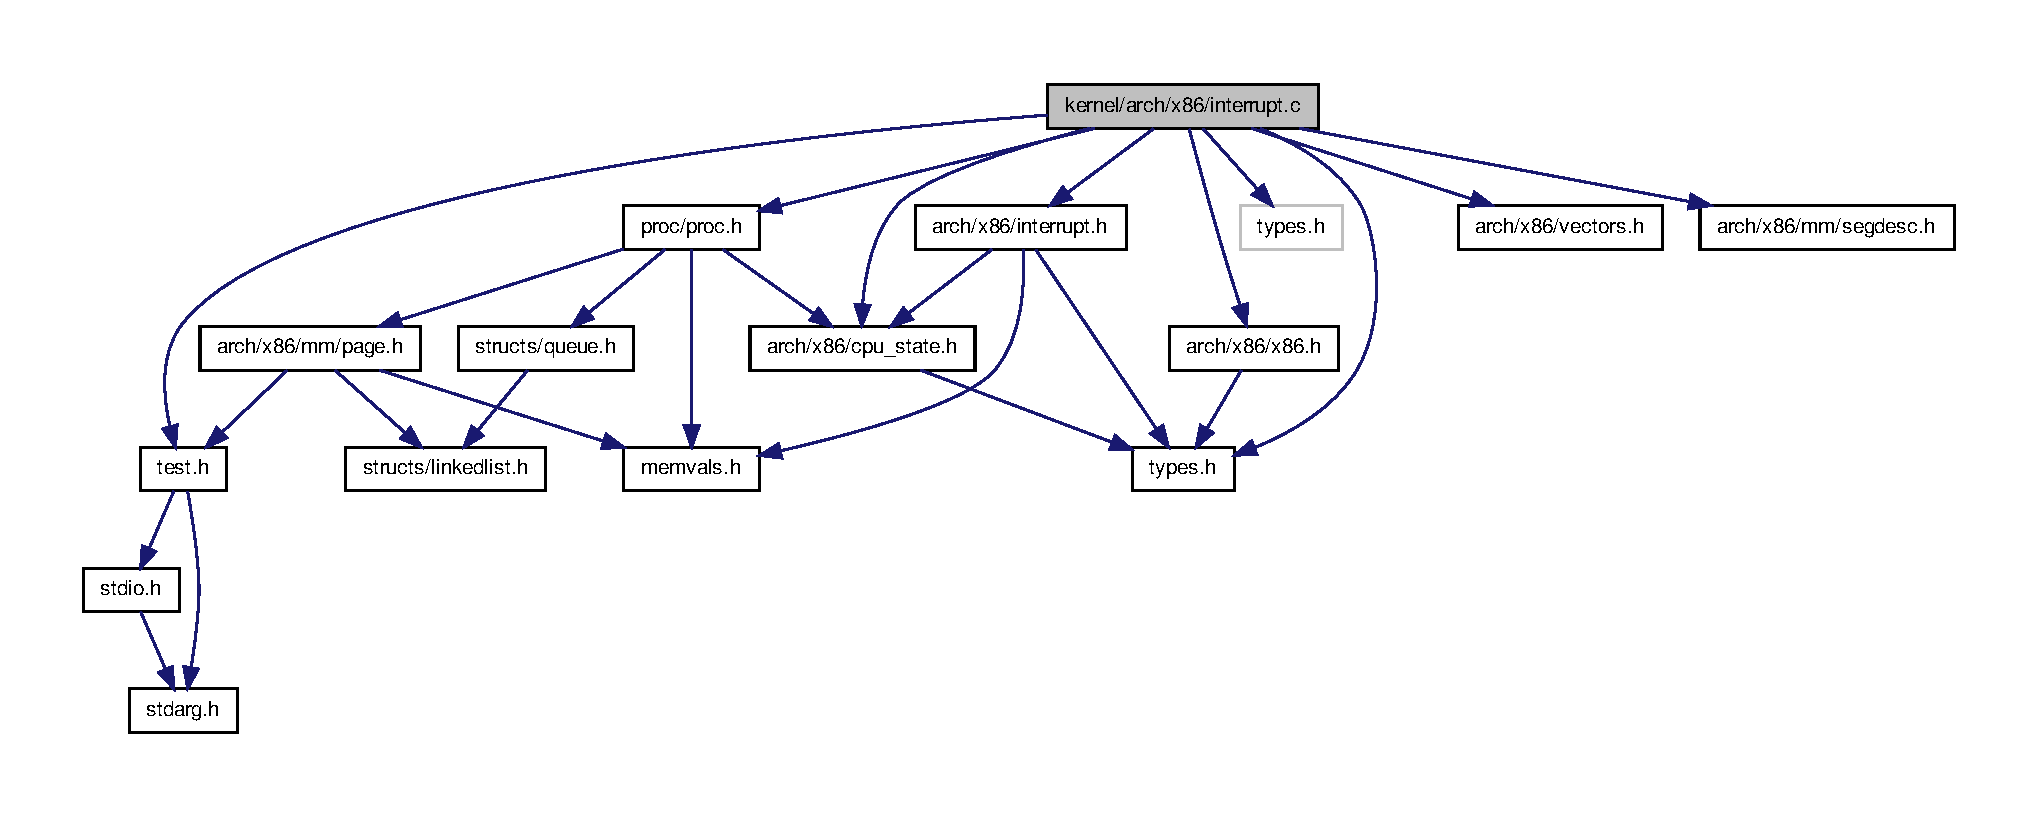
\includegraphics[width=350pt]{interrupt_8c__incl}
\end{center}
\end{figure}
\subsection*{\-Functions}
\begin{DoxyCompactItemize}
\item 
void \hyperlink{interrupt_8c_aec1d1c87cbfcb716257cc7c4f6766bd2}{trap} (void)
\item 
void \hyperlink{interrupt_8c_a164d38a0163ec2c36993b803b8c7fdcb}{idt\-\_\-init} (void)
\item 
void \hyperlink{interrupt_8c_a8d7db7dde7fc6c113d1f10578db13816}{register\-\_\-exception} (\hyperlink{types_8h_a435d1572bf3f880d55459d9805097f62}{uint32\-\_\-t} index, char $\ast$name, \hyperlink{types_8h_a273cf69d639a59973b6019625df33e30}{uint16\-\_\-t} present, void(handler)(void))
\item 
void \hyperlink{interrupt_8c_aae3db3a98d70c22944d98e61fa398938}{interrupt\-\_\-init} (void)
\item 
void \hyperlink{interrupt_8c_aee258f399635eb17537ee286417e141c}{map\-\_\-exception} (\hyperlink{types_8h_a435d1572bf3f880d55459d9805097f62}{uint32\-\_\-t} int\-\_\-index, \hyperlink{structcpu__state__t}{cpu\-\_\-state\-\_\-t} $\ast$cpu\-\_\-state)
\item 
\hyperlink{types_8h_a435d1572bf3f880d55459d9805097f62}{uint32\-\_\-t} \hyperlink{interrupt_8c_a5ca993690237b19d024337e30eecea6c}{page\-\_\-fault\-\_\-handler} (\hyperlink{structcpu__state__t}{cpu\-\_\-state\-\_\-t} $\ast$cpu\-\_\-state)
\end{DoxyCompactItemize}
\subsection*{\-Variables}
\begin{DoxyCompactItemize}
\item 
gatedesc \hyperlink{interrupt_8c_a5d1792166c76d20f9054b3bda93be7c4}{idt} \mbox{[}64\mbox{]}
\item 
char $\ast$ \hyperlink{interrupt_8c_a555133898405bfedf4422c9f76a58875}{x86\-\_\-exception\-\_\-names} \mbox{[}$\,$\mbox{]}
\item 
\hyperlink{interrupt_8c_aeb98d34fe8825c3bd7d199f9f55ec66f}{int\-\_\-generic}
\end{DoxyCompactItemize}


\subsection{\-Function \-Documentation}
\hypertarget{interrupt_8c_a164d38a0163ec2c36993b803b8c7fdcb}{\index{interrupt.\-c@{interrupt.\-c}!idt\-\_\-init@{idt\-\_\-init}}
\index{idt\-\_\-init@{idt\-\_\-init}!interrupt.c@{interrupt.\-c}}
\subsubsection[{idt\-\_\-init}]{\setlength{\rightskip}{0pt plus 5cm}void {\bf idt\-\_\-init} (
\begin{DoxyParamCaption}
\item[{void}]{}
\end{DoxyParamCaption}
)}}\label{interrupt_8c_a164d38a0163ec2c36993b803b8c7fdcb}


\-Definition at line 60 of file interrupt.\-c.

\hypertarget{interrupt_8c_aae3db3a98d70c22944d98e61fa398938}{\index{interrupt.\-c@{interrupt.\-c}!interrupt\-\_\-init@{interrupt\-\_\-init}}
\index{interrupt\-\_\-init@{interrupt\-\_\-init}!interrupt.c@{interrupt.\-c}}
\subsubsection[{interrupt\-\_\-init}]{\setlength{\rightskip}{0pt plus 5cm}void {\bf interrupt\-\_\-init} (
\begin{DoxyParamCaption}
\item[{void}]{}
\end{DoxyParamCaption}
)}}\label{interrupt_8c_aae3db3a98d70c22944d98e61fa398938}


\-Definition at line 160 of file interrupt.\-c.

\hypertarget{interrupt_8c_aee258f399635eb17537ee286417e141c}{\index{interrupt.\-c@{interrupt.\-c}!map\-\_\-exception@{map\-\_\-exception}}
\index{map\-\_\-exception@{map\-\_\-exception}!interrupt.c@{interrupt.\-c}}
\subsubsection[{map\-\_\-exception}]{\setlength{\rightskip}{0pt plus 5cm}void {\bf map\-\_\-exception} (
\begin{DoxyParamCaption}
\item[{{\bf uint32\-\_\-t}}]{int\-\_\-index, }
\item[{{\bf cpu\-\_\-state\-\_\-t} $\ast$}]{cpu\-\_\-state}
\end{DoxyParamCaption}
)}}\label{interrupt_8c_aee258f399635eb17537ee286417e141c}


\-Definition at line 166 of file interrupt.\-c.

\hypertarget{interrupt_8c_a5ca993690237b19d024337e30eecea6c}{\index{interrupt.\-c@{interrupt.\-c}!page\-\_\-fault\-\_\-handler@{page\-\_\-fault\-\_\-handler}}
\index{page\-\_\-fault\-\_\-handler@{page\-\_\-fault\-\_\-handler}!interrupt.c@{interrupt.\-c}}
\subsubsection[{page\-\_\-fault\-\_\-handler}]{\setlength{\rightskip}{0pt plus 5cm}{\bf uint32\-\_\-t} {\bf page\-\_\-fault\-\_\-handler} (
\begin{DoxyParamCaption}
\item[{{\bf cpu\-\_\-state\-\_\-t} $\ast$}]{cpu\-\_\-state}
\end{DoxyParamCaption}
)}}\label{interrupt_8c_a5ca993690237b19d024337e30eecea6c}


\-Definition at line 195 of file interrupt.\-c.

\hypertarget{interrupt_8c_a8d7db7dde7fc6c113d1f10578db13816}{\index{interrupt.\-c@{interrupt.\-c}!register\-\_\-exception@{register\-\_\-exception}}
\index{register\-\_\-exception@{register\-\_\-exception}!interrupt.c@{interrupt.\-c}}
\subsubsection[{register\-\_\-exception}]{\setlength{\rightskip}{0pt plus 5cm}void {\bf register\-\_\-exception} (
\begin{DoxyParamCaption}
\item[{{\bf uint32\-\_\-t}}]{index, }
\item[{char $\ast$}]{name, }
\item[{{\bf uint16\-\_\-t}}]{present, }
\item[{void(handler)(void)}]{}
\end{DoxyParamCaption}
)}}\label{interrupt_8c_a8d7db7dde7fc6c113d1f10578db13816}


\-Definition at line 154 of file interrupt.\-c.

\hypertarget{interrupt_8c_aec1d1c87cbfcb716257cc7c4f6766bd2}{\index{interrupt.\-c@{interrupt.\-c}!trap@{trap}}
\index{trap@{trap}!interrupt.c@{interrupt.\-c}}
\subsubsection[{trap}]{\setlength{\rightskip}{0pt plus 5cm}void {\bf trap} (
\begin{DoxyParamCaption}
\item[{void}]{}
\end{DoxyParamCaption}
)}}\label{interrupt_8c_aec1d1c87cbfcb716257cc7c4f6766bd2}


\-Definition at line 44 of file interrupt.\-c.



\subsection{\-Variable \-Documentation}
\hypertarget{interrupt_8c_a5d1792166c76d20f9054b3bda93be7c4}{\index{interrupt.\-c@{interrupt.\-c}!idt@{idt}}
\index{idt@{idt}!interrupt.c@{interrupt.\-c}}
\subsubsection[{idt}]{\setlength{\rightskip}{0pt plus 5cm}gatedesc {\bf idt}}}\label{interrupt_8c_a5d1792166c76d20f9054b3bda93be7c4}
\hyperlink{interrupt_8h}{include/arch/x86/interrupt.\-h} \-C\-A\-T\-Reloaded (\-C) \-Copyrights 2011 \href{http://catreloaded.net}{\tt http\-://catreloaded.\-net}

\begin{DoxyDate}{\-Date}
27 \-Sept, 2012 
\end{DoxyDate}


\-Definition at line 19 of file interrupt.\-c.

\hypertarget{interrupt_8c_aeb98d34fe8825c3bd7d199f9f55ec66f}{\index{interrupt.\-c@{interrupt.\-c}!int\-\_\-generic@{int\-\_\-generic}}
\index{int\-\_\-generic@{int\-\_\-generic}!interrupt.c@{interrupt.\-c}}
\subsubsection[{int\-\_\-generic}]{\setlength{\rightskip}{0pt plus 5cm}{\bf int\-\_\-generic}}}\label{interrupt_8c_aeb98d34fe8825c3bd7d199f9f55ec66f}
\hypertarget{interrupt_8c_a555133898405bfedf4422c9f76a58875}{\index{interrupt.\-c@{interrupt.\-c}!x86\-\_\-exception\-\_\-names@{x86\-\_\-exception\-\_\-names}}
\index{x86\-\_\-exception\-\_\-names@{x86\-\_\-exception\-\_\-names}!interrupt.c@{interrupt.\-c}}
\subsubsection[{x86\-\_\-exception\-\_\-names}]{\setlength{\rightskip}{0pt plus 5cm}char$\ast$ {\bf x86\-\_\-exception\-\_\-names}\mbox{[}$\,$\mbox{]}}}\label{interrupt_8c_a555133898405bfedf4422c9f76a58875}
{\bfseries \-Initial value\-:}
\begin{DoxyCode}
{
        "Divide Error #DE",
        "Debug",
        "NMI",
        "Breakpoint #BP",
        "Overflow #OV",
        "Bound Range Exceeded #BR",
        "Undefined Opcode",
        "Device not avalible",
        "Double fault",
        "Coprocessor segment overrun",
        "Invalid TSS",
        "Segment not present",
        "Stack Segment Fault",
        "General Protection",
        "Page Fault",
        "\0",
        "x87 FPU error",
        "Alignment Mask",
        "Machine Check",
        "SIMD exception"
        }
\end{DoxyCode}


\-Definition at line 20 of file interrupt.\-c.


\hypertarget{init__mem_8c}{\section{kernel/arch/x86/mm/init\-\_\-mem.c \-File \-Reference}
\label{init__mem_8c}\index{kernel/arch/x86/mm/init\-\_\-mem.\-c@{kernel/arch/x86/mm/init\-\_\-mem.\-c}}
}
{\ttfamily \#include $<$types.\-h$>$}\*
{\ttfamily \#include $<$arch/x86/x86.\-h$>$}\*
{\ttfamily \#include $<$memvals.\-h$>$}\*
{\ttfamily \#include $<$cmos.\-h$>$}\*
{\ttfamily \#include $<$string.\-h$>$}\*
{\ttfamily \#include $<$arch/x86/processor.\-h$>$}\*
{\ttfamily \#include $<$arch/x86/mm/page.\-h$>$}\*
{\ttfamily \#include $<$arch/x86/interrupt.\-h$>$}\*
{\ttfamily \#include $<$arch/x86/cpu\-\_\-state.\-h$>$}\*
{\ttfamily \#include $<$proc/proc.\-h$>$}\*
\-Include dependency graph for init\-\_\-mem.\-c\-:\nopagebreak
\begin{figure}[H]
\begin{center}
\leavevmode
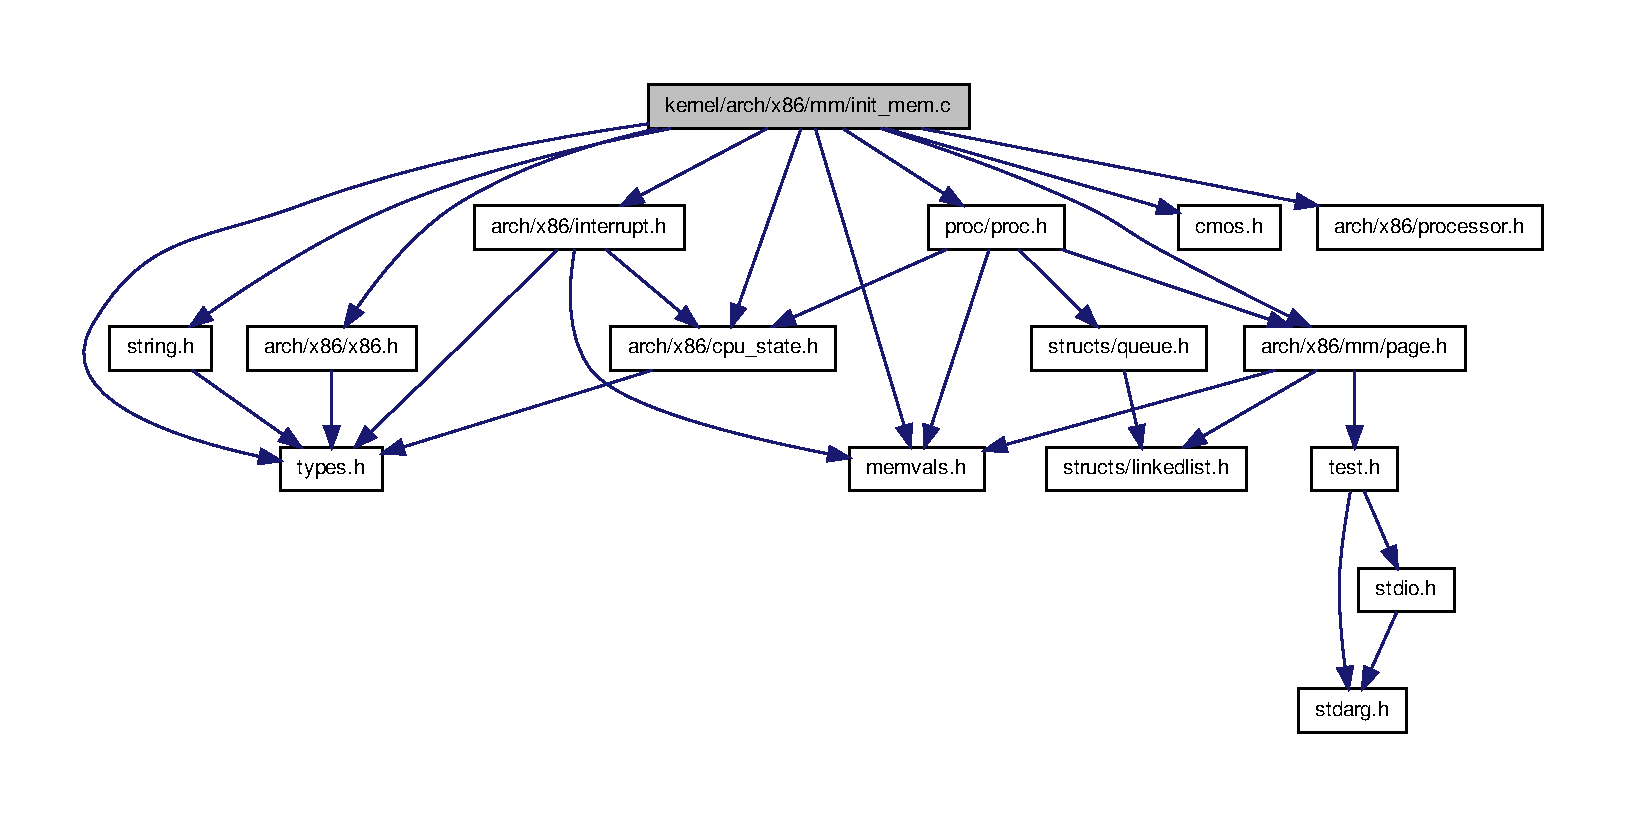
\includegraphics[width=350pt]{init__mem_8c__incl}
\end{center}
\end{figure}
\subsection*{\-Functions}
\begin{DoxyCompactItemize}
\item 
static \hyperlink{types_8h_a435d1572bf3f880d55459d9805097f62}{uint32\-\_\-t} \hyperlink{init__mem_8c_ae211c9a7f35cbed9323ae43a16e69737}{x86\-\_\-read\-\_\-mem\-\_\-size} (int x)
\item 
void \hyperlink{init__mem_8c_a1ba69b97e0fef308cbf209384a7fcd81}{scan\-\_\-memory} (void)
\item 
static void $\ast$ \hyperlink{init__mem_8c_a9762d88ec8eee643ee3527ae5f765cd4}{allocate} (\hyperlink{types_8h_a435d1572bf3f880d55459d9805097f62}{uint32\-\_\-t} n, \hyperlink{types_8h_a435d1572bf3f880d55459d9805097f62}{uint32\-\_\-t} align)
\item 
void \hyperlink{init__mem_8c_aed3ab9d856a5001fb79add2f66523234}{init\-\_\-tss} (void)
\item 
void \hyperlink{init__mem_8c_ab51e89d6798c133feb72e0546b330e6b}{x86\-\_\-setup\-\_\-memory} (void)
\end{DoxyCompactItemize}
\subsection*{\-Variables}
\begin{DoxyCompactItemize}
\item 
\hyperlink{types_8h_a435d1572bf3f880d55459d9805097f62}{uint32\-\_\-t} \hyperlink{init__mem_8c_a2eb17745f365b108bb5c8f0c727effa7}{max\-\_\-addr}
\item 
static \hyperlink{types_8h_a435d1572bf3f880d55459d9805097f62}{uint32\-\_\-t} \hyperlink{init__mem_8c_a5ba2f6f78705b63f0788f9b85f7f104c}{mem\-\_\-base}
\item 
static \hyperlink{types_8h_a435d1572bf3f880d55459d9805097f62}{uint32\-\_\-t} \hyperlink{init__mem_8c_a6d82d3a092ab3261207c2172340f057d}{ext\-\_\-base}
\item 
char $\ast$ \hyperlink{init__mem_8c_a39aa9990303c751420729e015f952dfb}{next\-\_\-free} = 0
\item 
static \hyperlink{types_8h_a435d1572bf3f880d55459d9805097f62}{uint32\-\_\-t} \hyperlink{init__mem_8c_af0ee28fa211c2bf5554596d9dcabd2bd}{alloc\-\_\-lock} = 0
\item 
struct \hyperlink{structPage}{\-Page} $\ast$ \hyperlink{init__mem_8c_a5c8561a52c4cda29a9be7dc7be92c771}{pages}
\item 
\hyperlink{proc_8h_abcae78bfd085fccd601f7cc568946453}{proc\-\_\-t} $\ast$ \hyperlink{init__mem_8c_a432b7b292b7d2423daf04aceac8924e6}{proc\-\_\-table}
\item 
struct \hyperlink{structSegdesc}{\-Segdesc} \hyperlink{init__mem_8c_a362a86eab2f1d332cf898b80741c89c9}{catgdt} \mbox{[}$\,$\mbox{]}
\item 
struct \hyperlink{structGdtdesc}{\-Gdtdesc} \hyperlink{init__mem_8c_a061803623c40821bfc4b422fa7b7454b}{gdtdesc}
\item 
\hyperlink{interrupt_8h_a81398f7aecfca5502a385160a0f84f7a}{\-Idtdesc} \hyperlink{init__mem_8c_a17f4900711fa847fd29c463f7f795b4a}{idtdesc}
\item 
tss\-\_\-t \hyperlink{init__mem_8c_aa24f361c0407c2ed810edfa9ef76da41}{tss}
\end{DoxyCompactItemize}


\subsection{\-Function \-Documentation}
\hypertarget{init__mem_8c_a9762d88ec8eee643ee3527ae5f765cd4}{\index{init\-\_\-mem.\-c@{init\-\_\-mem.\-c}!allocate@{allocate}}
\index{allocate@{allocate}!init_mem.c@{init\-\_\-mem.\-c}}
\subsubsection[{allocate}]{\setlength{\rightskip}{0pt plus 5cm}static void$\ast$ {\bf allocate} (
\begin{DoxyParamCaption}
\item[{{\bf uint32\-\_\-t}}]{n, }
\item[{{\bf uint32\-\_\-t}}]{align}
\end{DoxyParamCaption}
)\hspace{0.3cm}{\ttfamily  \mbox{[}static\mbox{]}}}}\label{init__mem_8c_a9762d88ec8eee643ee3527ae5f765cd4}


\-Definition at line 96 of file init\-\_\-mem.\-c.

\hypertarget{init__mem_8c_aed3ab9d856a5001fb79add2f66523234}{\index{init\-\_\-mem.\-c@{init\-\_\-mem.\-c}!init\-\_\-tss@{init\-\_\-tss}}
\index{init\-\_\-tss@{init\-\_\-tss}!init_mem.c@{init\-\_\-mem.\-c}}
\subsubsection[{init\-\_\-tss}]{\setlength{\rightskip}{0pt plus 5cm}void {\bf init\-\_\-tss} (
\begin{DoxyParamCaption}
\item[{void}]{}
\end{DoxyParamCaption}
)}}\label{init__mem_8c_aed3ab9d856a5001fb79add2f66523234}


\-Definition at line 118 of file init\-\_\-mem.\-c.

\hypertarget{init__mem_8c_a1ba69b97e0fef308cbf209384a7fcd81}{\index{init\-\_\-mem.\-c@{init\-\_\-mem.\-c}!scan\-\_\-memory@{scan\-\_\-memory}}
\index{scan\-\_\-memory@{scan\-\_\-memory}!init_mem.c@{init\-\_\-mem.\-c}}
\subsubsection[{scan\-\_\-memory}]{\setlength{\rightskip}{0pt plus 5cm}void {\bf scan\-\_\-memory} (
\begin{DoxyParamCaption}
\item[{void}]{}
\end{DoxyParamCaption}
)}}\label{init__mem_8c_a1ba69b97e0fef308cbf209384a7fcd81}


\-Definition at line 75 of file init\-\_\-mem.\-c.

\hypertarget{init__mem_8c_ae211c9a7f35cbed9323ae43a16e69737}{\index{init\-\_\-mem.\-c@{init\-\_\-mem.\-c}!x86\-\_\-read\-\_\-mem\-\_\-size@{x86\-\_\-read\-\_\-mem\-\_\-size}}
\index{x86\-\_\-read\-\_\-mem\-\_\-size@{x86\-\_\-read\-\_\-mem\-\_\-size}!init_mem.c@{init\-\_\-mem.\-c}}
\subsubsection[{x86\-\_\-read\-\_\-mem\-\_\-size}]{\setlength{\rightskip}{0pt plus 5cm}static {\bf uint32\-\_\-t} {\bf x86\-\_\-read\-\_\-mem\-\_\-size} (
\begin{DoxyParamCaption}
\item[{int}]{x}
\end{DoxyParamCaption}
)\hspace{0.3cm}{\ttfamily  \mbox{[}static\mbox{]}}}}\label{init__mem_8c_ae211c9a7f35cbed9323ae43a16e69737}


\-Definition at line 70 of file init\-\_\-mem.\-c.

\hypertarget{init__mem_8c_ab51e89d6798c133feb72e0546b330e6b}{\index{init\-\_\-mem.\-c@{init\-\_\-mem.\-c}!x86\-\_\-setup\-\_\-memory@{x86\-\_\-setup\-\_\-memory}}
\index{x86\-\_\-setup\-\_\-memory@{x86\-\_\-setup\-\_\-memory}!init_mem.c@{init\-\_\-mem.\-c}}
\subsubsection[{x86\-\_\-setup\-\_\-memory}]{\setlength{\rightskip}{0pt plus 5cm}void {\bf x86\-\_\-setup\-\_\-memory} (
\begin{DoxyParamCaption}
\item[{void}]{}
\end{DoxyParamCaption}
)}}\label{init__mem_8c_ab51e89d6798c133feb72e0546b330e6b}
\-At this point paging is on 

\-Definition at line 131 of file init\-\_\-mem.\-c.



\subsection{\-Variable \-Documentation}
\hypertarget{init__mem_8c_af0ee28fa211c2bf5554596d9dcabd2bd}{\index{init\-\_\-mem.\-c@{init\-\_\-mem.\-c}!alloc\-\_\-lock@{alloc\-\_\-lock}}
\index{alloc\-\_\-lock@{alloc\-\_\-lock}!init_mem.c@{init\-\_\-mem.\-c}}
\subsubsection[{alloc\-\_\-lock}]{\setlength{\rightskip}{0pt plus 5cm}{\bf uint32\-\_\-t} {\bf alloc\-\_\-lock} = 0\hspace{0.3cm}{\ttfamily  \mbox{[}static\mbox{]}}}}\label{init__mem_8c_af0ee28fa211c2bf5554596d9dcabd2bd}


\-Definition at line 23 of file init\-\_\-mem.\-c.

\hypertarget{init__mem_8c_a362a86eab2f1d332cf898b80741c89c9}{\index{init\-\_\-mem.\-c@{init\-\_\-mem.\-c}!catgdt@{catgdt}}
\index{catgdt@{catgdt}!init_mem.c@{init\-\_\-mem.\-c}}
\subsubsection[{catgdt}]{\setlength{\rightskip}{0pt plus 5cm}struct {\bf \-Segdesc} {\bf catgdt}\mbox{[}$\,$\mbox{]}}}\label{init__mem_8c_a362a86eab2f1d332cf898b80741c89c9}
{\bfseries \-Initial value\-:}
\begin{DoxyCode}
 {
        
        SEG_NULL,
        
        [1] = SEGMENT(0xffffffff, 0, SEGACS_RW | SEGACS_X),
        
        [2] = SEGMENT(0xffffffff, 0, SEGACS_RW),
        
        [3] = SEGMENT(0xffffffff, 0x000000, SEGACS_RW | SEGACS_USR | SEGACS_X),
        
        [4] = SEGMENT(0xffffffff, 0x0, SEGACS_RW | SEGACS_USR),
        
        
        [5] = SEG_NULL
        

}
\end{DoxyCode}


\-Definition at line 37 of file init\-\_\-mem.\-c.

\hypertarget{init__mem_8c_a6d82d3a092ab3261207c2172340f057d}{\index{init\-\_\-mem.\-c@{init\-\_\-mem.\-c}!ext\-\_\-base@{ext\-\_\-base}}
\index{ext\-\_\-base@{ext\-\_\-base}!init_mem.c@{init\-\_\-mem.\-c}}
\subsubsection[{ext\-\_\-base}]{\setlength{\rightskip}{0pt plus 5cm}{\bf uint32\-\_\-t} {\bf ext\-\_\-base}\hspace{0.3cm}{\ttfamily  \mbox{[}static\mbox{]}}}}\label{init__mem_8c_a6d82d3a092ab3261207c2172340f057d}


\-Definition at line 21 of file init\-\_\-mem.\-c.

\hypertarget{init__mem_8c_a061803623c40821bfc4b422fa7b7454b}{\index{init\-\_\-mem.\-c@{init\-\_\-mem.\-c}!gdtdesc@{gdtdesc}}
\index{gdtdesc@{gdtdesc}!init_mem.c@{init\-\_\-mem.\-c}}
\subsubsection[{gdtdesc}]{\setlength{\rightskip}{0pt plus 5cm}struct {\bf \-Gdtdesc} {\bf gdtdesc}}}\label{init__mem_8c_a061803623c40821bfc4b422fa7b7454b}
{\bfseries \-Initial value\-:}
\begin{DoxyCode}
{
        sizeof(catgdt)-1,
        (unsigned long) catgdt

}
\end{DoxyCode}


\-Definition at line 55 of file init\-\_\-mem.\-c.

\hypertarget{init__mem_8c_a17f4900711fa847fd29c463f7f795b4a}{\index{init\-\_\-mem.\-c@{init\-\_\-mem.\-c}!idtdesc@{idtdesc}}
\index{idtdesc@{idtdesc}!init_mem.c@{init\-\_\-mem.\-c}}
\subsubsection[{idtdesc}]{\setlength{\rightskip}{0pt plus 5cm}{\bf \-Idtdesc} {\bf idtdesc}}}\label{init__mem_8c_a17f4900711fa847fd29c463f7f795b4a}
{\bfseries \-Initial value\-:}
\begin{DoxyCode}
 {
        (256*sizeof(gatedesc))-1,
        (unsigned long) idt

}
\end{DoxyCode}


\-Definition at line 61 of file init\-\_\-mem.\-c.

\hypertarget{init__mem_8c_a2eb17745f365b108bb5c8f0c727effa7}{\index{init\-\_\-mem.\-c@{init\-\_\-mem.\-c}!max\-\_\-addr@{max\-\_\-addr}}
\index{max\-\_\-addr@{max\-\_\-addr}!init_mem.c@{init\-\_\-mem.\-c}}
\subsubsection[{max\-\_\-addr}]{\setlength{\rightskip}{0pt plus 5cm}{\bf uint32\-\_\-t} {\bf max\-\_\-addr}}}\label{init__mem_8c_a2eb17745f365b108bb5c8f0c727effa7}


\-Definition at line 20 of file init\-\_\-mem.\-c.

\hypertarget{init__mem_8c_a5ba2f6f78705b63f0788f9b85f7f104c}{\index{init\-\_\-mem.\-c@{init\-\_\-mem.\-c}!mem\-\_\-base@{mem\-\_\-base}}
\index{mem\-\_\-base@{mem\-\_\-base}!init_mem.c@{init\-\_\-mem.\-c}}
\subsubsection[{mem\-\_\-base}]{\setlength{\rightskip}{0pt plus 5cm}{\bf uint32\-\_\-t} {\bf mem\-\_\-base}\hspace{0.3cm}{\ttfamily  \mbox{[}static\mbox{]}}}}\label{init__mem_8c_a5ba2f6f78705b63f0788f9b85f7f104c}


\-Definition at line 21 of file init\-\_\-mem.\-c.

\hypertarget{init__mem_8c_a39aa9990303c751420729e015f952dfb}{\index{init\-\_\-mem.\-c@{init\-\_\-mem.\-c}!next\-\_\-free@{next\-\_\-free}}
\index{next\-\_\-free@{next\-\_\-free}!init_mem.c@{init\-\_\-mem.\-c}}
\subsubsection[{next\-\_\-free}]{\setlength{\rightskip}{0pt plus 5cm}char$\ast$ {\bf next\-\_\-free} = 0}}\label{init__mem_8c_a39aa9990303c751420729e015f952dfb}


\-Definition at line 22 of file init\-\_\-mem.\-c.

\hypertarget{init__mem_8c_a5c8561a52c4cda29a9be7dc7be92c771}{\index{init\-\_\-mem.\-c@{init\-\_\-mem.\-c}!pages@{pages}}
\index{pages@{pages}!init_mem.c@{init\-\_\-mem.\-c}}
\subsubsection[{pages}]{\setlength{\rightskip}{0pt plus 5cm}struct {\bf \-Page}$\ast$ {\bf pages}}}\label{init__mem_8c_a5c8561a52c4cda29a9be7dc7be92c771}


\-Definition at line 17 of file page.\-c.

\hypertarget{init__mem_8c_a432b7b292b7d2423daf04aceac8924e6}{\index{init\-\_\-mem.\-c@{init\-\_\-mem.\-c}!proc\-\_\-table@{proc\-\_\-table}}
\index{proc\-\_\-table@{proc\-\_\-table}!init_mem.c@{init\-\_\-mem.\-c}}
\subsubsection[{proc\-\_\-table}]{\setlength{\rightskip}{0pt plus 5cm}{\bf proc\-\_\-t}$\ast$ {\bf proc\-\_\-table}}}\label{init__mem_8c_a432b7b292b7d2423daf04aceac8924e6}


\-Definition at line 13 of file proc.\-c.

\hypertarget{init__mem_8c_aa24f361c0407c2ed810edfa9ef76da41}{\index{init\-\_\-mem.\-c@{init\-\_\-mem.\-c}!tss@{tss}}
\index{tss@{tss}!init_mem.c@{init\-\_\-mem.\-c}}
\subsubsection[{tss}]{\setlength{\rightskip}{0pt plus 5cm}tss\-\_\-t {\bf tss}}}\label{init__mem_8c_aa24f361c0407c2ed810edfa9ef76da41}


\-Definition at line 67 of file init\-\_\-mem.\-c.


\hypertarget{page_8c}{\section{kernel/arch/x86/mm/page.c \-File \-Reference}
\label{page_8c}\index{kernel/arch/x86/mm/page.\-c@{kernel/arch/x86/mm/page.\-c}}
}
{\ttfamily \#include $<$types.\-h$>$}\*
{\ttfamily \#include $<$arch/x86/x86.\-h$>$}\*
{\ttfamily \#include $<$memvals.\-h$>$}\*
{\ttfamily \#include $<$string.\-h$>$}\*
{\ttfamily \#include $<$arch/x86/mm/page.\-h$>$}\*
\-Include dependency graph for page.\-c\-:\nopagebreak
\begin{figure}[H]
\begin{center}
\leavevmode
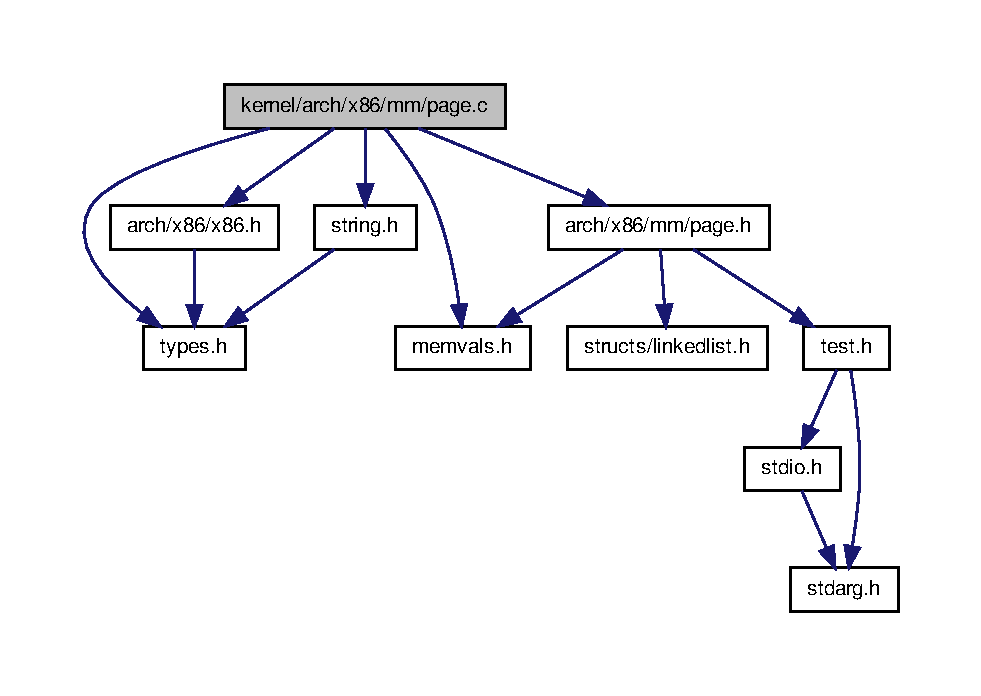
\includegraphics[width=350pt]{page_8c__incl}
\end{center}
\end{figure}
\subsection*{\-Functions}
\begin{DoxyCompactItemize}
\item 
void \hyperlink{page_8c_a3116202f5e2264b63f5a69f007287b9a}{x86\-\_\-paging\-\_\-init} (void)
\item 
void \hyperlink{page_8c_a47035fa680fdf11c7403445db4762728}{x86\-\_\-page\-\_\-init} (struct \hyperlink{structPage}{\-Page} $\ast$page)
\item 
int \hyperlink{page_8c_afdfcf53a6e442e1244205d5caa178dc1}{x86\-\_\-page\-\_\-alloc} (struct \hyperlink{structPage}{\-Page} $\ast$$\ast$page\-\_\-byref)
\item 
void \hyperlink{page_8c_abf1a7d08ef370ed140d68279466d16c2}{x86\-\_\-page\-\_\-free} (struct \hyperlink{structPage}{\-Page} $\ast$page)
\item 
void \hyperlink{page_8c_a0e4ecf1dbcf05554104e7f089e6eaa9b}{x86\-\_\-page\-\_\-detach} (struct \hyperlink{structPage}{\-Page} $\ast$page)
\item 
pte\-\_\-t $\ast$ \hyperlink{page_8c_a7a6381142371ad1ed883bc33683c68de}{x86\-\_\-pgdir\-\_\-find} (\hyperlink{page_8h_a1ae9855ac82633447ab53f25e49e1f62}{pde\-\_\-t} $\ast$pgdir, const void $\ast$va, int \hyperlink{init__mem_8c_a9762d88ec8eee643ee3527ae5f765cd4}{allocate})
\item 
struct \hyperlink{structPage}{\-Page} $\ast$ \hyperlink{page_8c_a90f1e53f745fbff067dd1d6e21e4a971}{x86\-\_\-page\-\_\-lookup} (\hyperlink{page_8h_a1ae9855ac82633447ab53f25e49e1f62}{pde\-\_\-t} $\ast$pgdir, void $\ast$va, pte\-\_\-t $\ast$$\ast$pte)
\item 
void \hyperlink{page_8c_a0094c45a39dd8369285c834af6512f53}{x86\-\_\-page\-\_\-remove} (\hyperlink{page_8h_a1ae9855ac82633447ab53f25e49e1f62}{pde\-\_\-t} $\ast$pgdir, void $\ast$va)
\item 
int \hyperlink{page_8c_ac8fee72731746be1776eee181b5c3d1f}{x86\-\_\-page\-\_\-insert} (\hyperlink{page_8h_a1ae9855ac82633447ab53f25e49e1f62}{pde\-\_\-t} $\ast$pgdir, struct \hyperlink{structPage}{\-Page} $\ast$page, void $\ast$va, \hyperlink{types_8h_a435d1572bf3f880d55459d9805097f62}{uint32\-\_\-t} perm)
\item 
void \hyperlink{page_8c_a72d597193a2cbbab7100effdf3e045df}{map\-\_\-segment\-\_\-page} (\hyperlink{page_8h_a1ae9855ac82633447ab53f25e49e1f62}{pde\-\_\-t} $\ast$pgdir, \hyperlink{types_8h_a53428b953a0ae6fba02a5b3596c867e0}{vaddr\-\_\-t} linear, \hyperlink{types_8h_a7c94ea6f8948649f8d181ae55911eeaf}{size\-\_\-t} \hyperlink{memvals_8h_aaba88b24a21a6c70c895c0d55f4a69a0}{size}, \hyperlink{types_8h_a9f047c1f0917f6184a7a013d4b4277a6}{paddr\-\_\-t} physical, int perm)
\item 
void \hyperlink{page_8c_a3c2de2a5079f7f0854f1e2df482dbd99}{x86\-\_\-test\-\_\-pgdir} (void)
\end{DoxyCompactItemize}
\subsection*{\-Variables}
\begin{DoxyCompactItemize}
\item 
\hyperlink{types_8h_a435d1572bf3f880d55459d9805097f62}{uint32\-\_\-t} \hyperlink{page_8c_aa993bc236650aa405b01d00b7ca72904}{page\-\_\-count}
\item 
\hyperlink{page_8h_a1ae9855ac82633447ab53f25e49e1f62}{pde\-\_\-t} $\ast$ \hyperlink{page_8c_a8ffe8b80013a018b23501ea7a45b7870}{global\-\_\-pgdir}
\item 
\hyperlink{types_8h_a435d1572bf3f880d55459d9805097f62}{uint32\-\_\-t} \hyperlink{page_8c_a18cb6aa9c5285aa7411ebd96a283741e}{global\-\_\-cr3}
\item 
char $\ast$ \hyperlink{page_8c_a39aa9990303c751420729e015f952dfb}{next\-\_\-free}
\item 
struct \hyperlink{structPage}{\-Page} $\ast$ \hyperlink{page_8c_a5c8561a52c4cda29a9be7dc7be92c771}{pages}
\item 
static struct \-Page\-List \hyperlink{page_8c_a47458068a4a6404d82cdab009deb7343}{free\-\_\-pages}
\end{DoxyCompactItemize}


\subsection{\-Function \-Documentation}
\hypertarget{page_8c_a72d597193a2cbbab7100effdf3e045df}{\index{page.\-c@{page.\-c}!map\-\_\-segment\-\_\-page@{map\-\_\-segment\-\_\-page}}
\index{map\-\_\-segment\-\_\-page@{map\-\_\-segment\-\_\-page}!page.c@{page.\-c}}
\subsubsection[{map\-\_\-segment\-\_\-page}]{\setlength{\rightskip}{0pt plus 5cm}void {\bf map\-\_\-segment\-\_\-page} (
\begin{DoxyParamCaption}
\item[{{\bf pde\-\_\-t} $\ast$}]{pgdir, }
\item[{{\bf vaddr\-\_\-t}}]{linear, }
\item[{{\bf size\-\_\-t}}]{size, }
\item[{{\bf paddr\-\_\-t}}]{physical, }
\item[{int}]{perm}
\end{DoxyParamCaption}
)}}\label{page_8c_a72d597193a2cbbab7100effdf3e045df}


\-Definition at line 231 of file page.\-c.

\hypertarget{page_8c_afdfcf53a6e442e1244205d5caa178dc1}{\index{page.\-c@{page.\-c}!x86\-\_\-page\-\_\-alloc@{x86\-\_\-page\-\_\-alloc}}
\index{x86\-\_\-page\-\_\-alloc@{x86\-\_\-page\-\_\-alloc}!page.c@{page.\-c}}
\subsubsection[{x86\-\_\-page\-\_\-alloc}]{\setlength{\rightskip}{0pt plus 5cm}int {\bf x86\-\_\-page\-\_\-alloc} (
\begin{DoxyParamCaption}
\item[{struct {\bf \-Page} $\ast$$\ast$}]{page\-\_\-byref}
\end{DoxyParamCaption}
)}}\label{page_8c_afdfcf53a6e442e1244205d5caa178dc1}


\-Definition at line 83 of file page.\-c.

\hypertarget{page_8c_a0e4ecf1dbcf05554104e7f089e6eaa9b}{\index{page.\-c@{page.\-c}!x86\-\_\-page\-\_\-detach@{x86\-\_\-page\-\_\-detach}}
\index{x86\-\_\-page\-\_\-detach@{x86\-\_\-page\-\_\-detach}!page.c@{page.\-c}}
\subsubsection[{x86\-\_\-page\-\_\-detach}]{\setlength{\rightskip}{0pt plus 5cm}void {\bf x86\-\_\-page\-\_\-detach} (
\begin{DoxyParamCaption}
\item[{struct {\bf \-Page} $\ast$}]{page}
\end{DoxyParamCaption}
)}}\label{page_8c_a0e4ecf1dbcf05554104e7f089e6eaa9b}


\-Definition at line 112 of file page.\-c.

\hypertarget{page_8c_abf1a7d08ef370ed140d68279466d16c2}{\index{page.\-c@{page.\-c}!x86\-\_\-page\-\_\-free@{x86\-\_\-page\-\_\-free}}
\index{x86\-\_\-page\-\_\-free@{x86\-\_\-page\-\_\-free}!page.c@{page.\-c}}
\subsubsection[{x86\-\_\-page\-\_\-free}]{\setlength{\rightskip}{0pt plus 5cm}void {\bf x86\-\_\-page\-\_\-free} (
\begin{DoxyParamCaption}
\item[{struct {\bf \-Page} $\ast$}]{page}
\end{DoxyParamCaption}
)}}\label{page_8c_abf1a7d08ef370ed140d68279466d16c2}


\-Definition at line 100 of file page.\-c.

\hypertarget{page_8c_a47035fa680fdf11c7403445db4762728}{\index{page.\-c@{page.\-c}!x86\-\_\-page\-\_\-init@{x86\-\_\-page\-\_\-init}}
\index{x86\-\_\-page\-\_\-init@{x86\-\_\-page\-\_\-init}!page.c@{page.\-c}}
\subsubsection[{x86\-\_\-page\-\_\-init}]{\setlength{\rightskip}{0pt plus 5cm}void {\bf x86\-\_\-page\-\_\-init} (
\begin{DoxyParamCaption}
\item[{struct {\bf \-Page} $\ast$}]{page}
\end{DoxyParamCaption}
)}}\label{page_8c_a47035fa680fdf11c7403445db4762728}


\-Definition at line 74 of file page.\-c.

\hypertarget{page_8c_ac8fee72731746be1776eee181b5c3d1f}{\index{page.\-c@{page.\-c}!x86\-\_\-page\-\_\-insert@{x86\-\_\-page\-\_\-insert}}
\index{x86\-\_\-page\-\_\-insert@{x86\-\_\-page\-\_\-insert}!page.c@{page.\-c}}
\subsubsection[{x86\-\_\-page\-\_\-insert}]{\setlength{\rightskip}{0pt plus 5cm}int {\bf x86\-\_\-page\-\_\-insert} (
\begin{DoxyParamCaption}
\item[{{\bf pde\-\_\-t} $\ast$}]{pgdir, }
\item[{struct {\bf \-Page} $\ast$}]{page, }
\item[{void $\ast$}]{va, }
\item[{{\bf uint32\-\_\-t}}]{perm}
\end{DoxyParamCaption}
)}}\label{page_8c_ac8fee72731746be1776eee181b5c3d1f}


\-Definition at line 184 of file page.\-c.

\hypertarget{page_8c_a90f1e53f745fbff067dd1d6e21e4a971}{\index{page.\-c@{page.\-c}!x86\-\_\-page\-\_\-lookup@{x86\-\_\-page\-\_\-lookup}}
\index{x86\-\_\-page\-\_\-lookup@{x86\-\_\-page\-\_\-lookup}!page.c@{page.\-c}}
\subsubsection[{x86\-\_\-page\-\_\-lookup}]{\setlength{\rightskip}{0pt plus 5cm}struct {\bf \-Page}$\ast$ {\bf x86\-\_\-page\-\_\-lookup} (
\begin{DoxyParamCaption}
\item[{{\bf pde\-\_\-t} $\ast$}]{pgdir, }
\item[{void $\ast$}]{va, }
\item[{pte\-\_\-t $\ast$$\ast$}]{pte}
\end{DoxyParamCaption}
)\hspace{0.3cm}{\ttfamily  \mbox{[}read\mbox{]}}}}\label{page_8c_a90f1e53f745fbff067dd1d6e21e4a971}


\-Definition at line 154 of file page.\-c.

\hypertarget{page_8c_a0094c45a39dd8369285c834af6512f53}{\index{page.\-c@{page.\-c}!x86\-\_\-page\-\_\-remove@{x86\-\_\-page\-\_\-remove}}
\index{x86\-\_\-page\-\_\-remove@{x86\-\_\-page\-\_\-remove}!page.c@{page.\-c}}
\subsubsection[{x86\-\_\-page\-\_\-remove}]{\setlength{\rightskip}{0pt plus 5cm}void {\bf x86\-\_\-page\-\_\-remove} (
\begin{DoxyParamCaption}
\item[{{\bf pde\-\_\-t} $\ast$}]{pgdir, }
\item[{void $\ast$}]{va}
\end{DoxyParamCaption}
)}}\label{page_8c_a0094c45a39dd8369285c834af6512f53}


\-Definition at line 170 of file page.\-c.

\hypertarget{page_8c_a3116202f5e2264b63f5a69f007287b9a}{\index{page.\-c@{page.\-c}!x86\-\_\-paging\-\_\-init@{x86\-\_\-paging\-\_\-init}}
\index{x86\-\_\-paging\-\_\-init@{x86\-\_\-paging\-\_\-init}!page.c@{page.\-c}}
\subsubsection[{x86\-\_\-paging\-\_\-init}]{\setlength{\rightskip}{0pt plus 5cm}void {\bf x86\-\_\-paging\-\_\-init} (
\begin{DoxyParamCaption}
\item[{void}]{}
\end{DoxyParamCaption}
)}}\label{page_8c_a3116202f5e2264b63f5a69f007287b9a}


\-Definition at line 26 of file page.\-c.

\hypertarget{page_8c_a7a6381142371ad1ed883bc33683c68de}{\index{page.\-c@{page.\-c}!x86\-\_\-pgdir\-\_\-find@{x86\-\_\-pgdir\-\_\-find}}
\index{x86\-\_\-pgdir\-\_\-find@{x86\-\_\-pgdir\-\_\-find}!page.c@{page.\-c}}
\subsubsection[{x86\-\_\-pgdir\-\_\-find}]{\setlength{\rightskip}{0pt plus 5cm}pte\-\_\-t$\ast$ {\bf x86\-\_\-pgdir\-\_\-find} (
\begin{DoxyParamCaption}
\item[{{\bf pde\-\_\-t} $\ast$}]{pgdir, }
\item[{const void $\ast$}]{va, }
\item[{int}]{allocate}
\end{DoxyParamCaption}
)}}\label{page_8c_a7a6381142371ad1ed883bc33683c68de}


\-Definition at line 126 of file page.\-c.

\hypertarget{page_8c_a3c2de2a5079f7f0854f1e2df482dbd99}{\index{page.\-c@{page.\-c}!x86\-\_\-test\-\_\-pgdir@{x86\-\_\-test\-\_\-pgdir}}
\index{x86\-\_\-test\-\_\-pgdir@{x86\-\_\-test\-\_\-pgdir}!page.c@{page.\-c}}
\subsubsection[{x86\-\_\-test\-\_\-pgdir}]{\setlength{\rightskip}{0pt plus 5cm}void {\bf x86\-\_\-test\-\_\-pgdir} (
\begin{DoxyParamCaption}
\item[{void}]{}
\end{DoxyParamCaption}
)}}\label{page_8c_a3c2de2a5079f7f0854f1e2df482dbd99}


\-Definition at line 250 of file page.\-c.



\subsection{\-Variable \-Documentation}
\hypertarget{page_8c_a47458068a4a6404d82cdab009deb7343}{\index{page.\-c@{page.\-c}!free\-\_\-pages@{free\-\_\-pages}}
\index{free\-\_\-pages@{free\-\_\-pages}!page.c@{page.\-c}}
\subsubsection[{free\-\_\-pages}]{\setlength{\rightskip}{0pt plus 5cm}struct \-Page\-List {\bf free\-\_\-pages}\hspace{0.3cm}{\ttfamily  \mbox{[}static\mbox{]}}}}\label{page_8c_a47458068a4a6404d82cdab009deb7343}


\-Definition at line 19 of file page.\-c.

\hypertarget{page_8c_a18cb6aa9c5285aa7411ebd96a283741e}{\index{page.\-c@{page.\-c}!global\-\_\-cr3@{global\-\_\-cr3}}
\index{global\-\_\-cr3@{global\-\_\-cr3}!page.c@{page.\-c}}
\subsubsection[{global\-\_\-cr3}]{\setlength{\rightskip}{0pt plus 5cm}{\bf uint32\-\_\-t} {\bf global\-\_\-cr3}}}\label{page_8c_a18cb6aa9c5285aa7411ebd96a283741e}


\-Definition at line 14 of file page.\-c.

\hypertarget{page_8c_a8ffe8b80013a018b23501ea7a45b7870}{\index{page.\-c@{page.\-c}!global\-\_\-pgdir@{global\-\_\-pgdir}}
\index{global\-\_\-pgdir@{global\-\_\-pgdir}!page.c@{page.\-c}}
\subsubsection[{global\-\_\-pgdir}]{\setlength{\rightskip}{0pt plus 5cm}{\bf pde\-\_\-t}$\ast$ {\bf global\-\_\-pgdir}}}\label{page_8c_a8ffe8b80013a018b23501ea7a45b7870}


\-Definition at line 13 of file page.\-c.

\hypertarget{page_8c_a39aa9990303c751420729e015f952dfb}{\index{page.\-c@{page.\-c}!next\-\_\-free@{next\-\_\-free}}
\index{next\-\_\-free@{next\-\_\-free}!page.c@{page.\-c}}
\subsubsection[{next\-\_\-free}]{\setlength{\rightskip}{0pt plus 5cm}char$\ast$ {\bf next\-\_\-free}}}\label{page_8c_a39aa9990303c751420729e015f952dfb}


\-Definition at line 22 of file init\-\_\-mem.\-c.

\hypertarget{page_8c_aa993bc236650aa405b01d00b7ca72904}{\index{page.\-c@{page.\-c}!page\-\_\-count@{page\-\_\-count}}
\index{page\-\_\-count@{page\-\_\-count}!page.c@{page.\-c}}
\subsubsection[{page\-\_\-count}]{\setlength{\rightskip}{0pt plus 5cm}{\bf uint32\-\_\-t} {\bf page\-\_\-count}}}\label{page_8c_aa993bc236650aa405b01d00b7ca72904}


\-Definition at line 12 of file page.\-c.

\hypertarget{page_8c_a5c8561a52c4cda29a9be7dc7be92c771}{\index{page.\-c@{page.\-c}!pages@{pages}}
\index{pages@{pages}!page.c@{page.\-c}}
\subsubsection[{pages}]{\setlength{\rightskip}{0pt plus 5cm}struct {\bf \-Page}$\ast$ {\bf pages}}}\label{page_8c_a5c8561a52c4cda29a9be7dc7be92c771}


\-Definition at line 17 of file page.\-c.


\hypertarget{cli_8c}{\section{kernel/cli.c \-File \-Reference}
\label{cli_8c}\index{kernel/cli.\-c@{kernel/cli.\-c}}
}
{\ttfamily \#include $<$types.\-h$>$}\*
{\ttfamily \#include $<$arch/x86/x86.\-h$>$}\*
{\ttfamily \#include $<$cli.\-h$>$}\*
{\ttfamily \#include $<$kbc.\-h$>$}\*
{\ttfamily \#include $<$video.\-h$>$}\*
{\ttfamily \#include $<$stdio.\-h$>$}\*
\-Include dependency graph for cli.\-c\-:\nopagebreak
\begin{figure}[H]
\begin{center}
\leavevmode
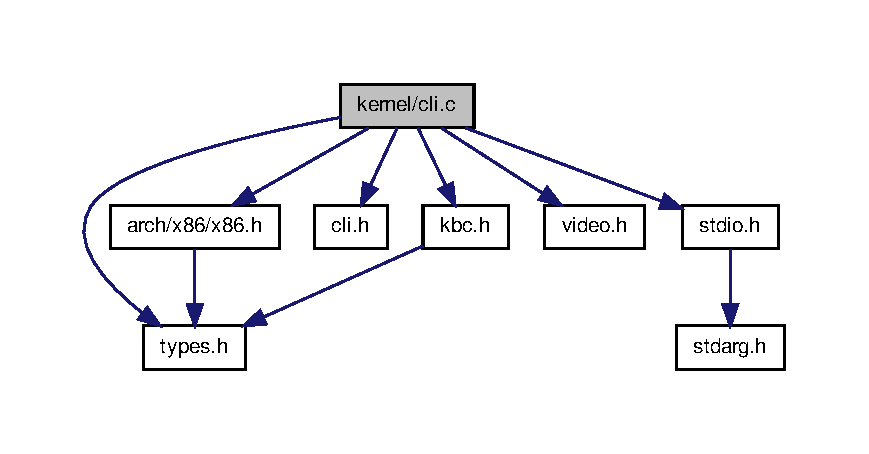
\includegraphics[width=350pt]{cli_8c__incl}
\end{center}
\end{figure}
\subsection*{\-Functions}
\begin{DoxyCompactItemize}
\item 
void \hyperlink{cli_8c_acadd2a5d99d952e55a4580dbc8f8739d}{console\-\_\-init} (void)
\item 
void \hyperlink{cli_8c_a3c8b2e35ff573401b1df8d0938cf75e6}{console\-\_\-interrupt} (int($\ast$intr)(void))
\item 
void \hyperlink{cli_8c_aa458c825fb8701dc71639422d2a03385}{console\-\_\-clear} (void)
\item 
int \hyperlink{cli_8c_a9b3ba9ca613021d6954ade2927d8d56e}{console\-\_\-getc} (void)
\item 
void \hyperlink{cli_8c_ad3429ca65a1b6f39eed6d2f9f795586b}{console\-\_\-putc} (int c)
\item 
void \hyperlink{cli_8c_a77246c715d47b2f9782c230ca981952e}{putchr} (int c)
\item 
int \hyperlink{cli_8c_a3e29caa20f7cffe18f410f01278905a8}{getchar} (void)
\end{DoxyCompactItemize}


\subsection{\-Function \-Documentation}
\hypertarget{cli_8c_aa458c825fb8701dc71639422d2a03385}{\index{cli.\-c@{cli.\-c}!console\-\_\-clear@{console\-\_\-clear}}
\index{console\-\_\-clear@{console\-\_\-clear}!cli.c@{cli.\-c}}
\subsubsection[{console\-\_\-clear}]{\setlength{\rightskip}{0pt plus 5cm}void {\bf console\-\_\-clear} (
\begin{DoxyParamCaption}
\item[{void}]{}
\end{DoxyParamCaption}
)}}\label{cli_8c_aa458c825fb8701dc71639422d2a03385}


\-Definition at line 28 of file cli.\-c.

\hypertarget{cli_8c_a9b3ba9ca613021d6954ade2927d8d56e}{\index{cli.\-c@{cli.\-c}!console\-\_\-getc@{console\-\_\-getc}}
\index{console\-\_\-getc@{console\-\_\-getc}!cli.c@{cli.\-c}}
\subsubsection[{console\-\_\-getc}]{\setlength{\rightskip}{0pt plus 5cm}int {\bf console\-\_\-getc} (
\begin{DoxyParamCaption}
\item[{void}]{}
\end{DoxyParamCaption}
)}}\label{cli_8c_a9b3ba9ca613021d6954ade2927d8d56e}


\-Definition at line 32 of file cli.\-c.

\hypertarget{cli_8c_acadd2a5d99d952e55a4580dbc8f8739d}{\index{cli.\-c@{cli.\-c}!console\-\_\-init@{console\-\_\-init}}
\index{console\-\_\-init@{console\-\_\-init}!cli.c@{cli.\-c}}
\subsubsection[{console\-\_\-init}]{\setlength{\rightskip}{0pt plus 5cm}void {\bf console\-\_\-init} (
\begin{DoxyParamCaption}
\item[{void}]{}
\end{DoxyParamCaption}
)}}\label{cli_8c_acadd2a5d99d952e55a4580dbc8f8739d}


\-Definition at line 8 of file cli.\-c.

\hypertarget{cli_8c_a3c8b2e35ff573401b1df8d0938cf75e6}{\index{cli.\-c@{cli.\-c}!console\-\_\-interrupt@{console\-\_\-interrupt}}
\index{console\-\_\-interrupt@{console\-\_\-interrupt}!cli.c@{cli.\-c}}
\subsubsection[{console\-\_\-interrupt}]{\setlength{\rightskip}{0pt plus 5cm}void {\bf console\-\_\-interrupt} (
\begin{DoxyParamCaption}
\item[{int($\ast$)(void)}]{intr}
\end{DoxyParamCaption}
)}}\label{cli_8c_a3c8b2e35ff573401b1df8d0938cf75e6}


\-Definition at line 16 of file cli.\-c.

\hypertarget{cli_8c_ad3429ca65a1b6f39eed6d2f9f795586b}{\index{cli.\-c@{cli.\-c}!console\-\_\-putc@{console\-\_\-putc}}
\index{console\-\_\-putc@{console\-\_\-putc}!cli.c@{cli.\-c}}
\subsubsection[{console\-\_\-putc}]{\setlength{\rightskip}{0pt plus 5cm}void {\bf console\-\_\-putc} (
\begin{DoxyParamCaption}
\item[{int}]{c}
\end{DoxyParamCaption}
)}}\label{cli_8c_ad3429ca65a1b6f39eed6d2f9f795586b}


\-Definition at line 45 of file cli.\-c.

\hypertarget{cli_8c_a3e29caa20f7cffe18f410f01278905a8}{\index{cli.\-c@{cli.\-c}!getchar@{getchar}}
\index{getchar@{getchar}!cli.c@{cli.\-c}}
\subsubsection[{getchar}]{\setlength{\rightskip}{0pt plus 5cm}int {\bf getchar} (
\begin{DoxyParamCaption}
\item[{void}]{}
\end{DoxyParamCaption}
)}}\label{cli_8c_a3e29caa20f7cffe18f410f01278905a8}


\-Definition at line 53 of file cli.\-c.

\hypertarget{cli_8c_a77246c715d47b2f9782c230ca981952e}{\index{cli.\-c@{cli.\-c}!putchr@{putchr}}
\index{putchr@{putchr}!cli.c@{cli.\-c}}
\subsubsection[{putchr}]{\setlength{\rightskip}{0pt plus 5cm}void {\bf putchr} (
\begin{DoxyParamCaption}
\item[{int}]{c}
\end{DoxyParamCaption}
)}}\label{cli_8c_a77246c715d47b2f9782c230ca981952e}


\-Definition at line 49 of file cli.\-c.


\hypertarget{cmos_8c}{\section{kernel/cmos.c \-File \-Reference}
\label{cmos_8c}\index{kernel/cmos.\-c@{kernel/cmos.\-c}}
}
{\ttfamily \#include $<$types.\-h$>$}\*
{\ttfamily \#include $<$arch/x86/x86.\-h$>$}\*
{\ttfamily \#include $<$cmos.\-h$>$}\*
\-Include dependency graph for cmos.\-c\-:\nopagebreak
\begin{figure}[H]
\begin{center}
\leavevmode
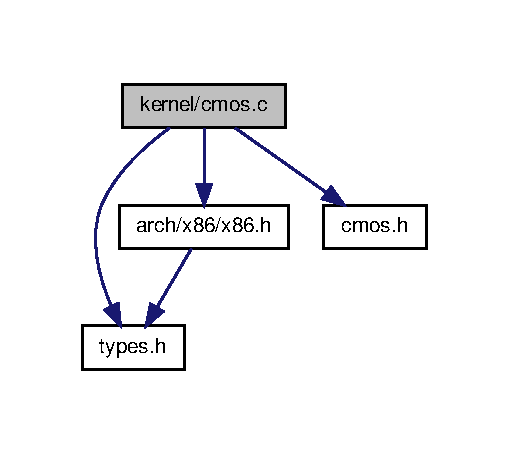
\includegraphics[width=244pt]{cmos_8c__incl}
\end{center}
\end{figure}
\subsection*{\-Functions}
\begin{DoxyCompactItemize}
\item 
\hyperlink{types_8h_aba7bc1797add20fe3efdf37ced1182c5}{uint8\-\_\-t} \hyperlink{cmos_8c_a79f13548024b22c9e29e1b1196dfa66d}{cmos\-\_\-set\-\_\-power\-\_\-stat} (\hyperlink{types_8h_aba7bc1797add20fe3efdf37ced1182c5}{uint8\-\_\-t} stat)
\item 
\hyperlink{types_8h_a435d1572bf3f880d55459d9805097f62}{uint32\-\_\-t} \hyperlink{cmos_8c_a56f6e4f404b4a6218c050c045d6732c3}{cmos\-\_\-get\-\_\-reg} (\hyperlink{types_8h_aba7bc1797add20fe3efdf37ced1182c5}{uint8\-\_\-t} value)
\item 
\hyperlink{types_8h_aba7bc1797add20fe3efdf37ced1182c5}{uint8\-\_\-t} \hyperlink{cmos_8c_a7d014a08169d9091ed83e880f491abe3}{cmos\-\_\-get\-\_\-time} (\hyperlink{types_8h_aba7bc1797add20fe3efdf37ced1182c5}{uint8\-\_\-t} value)
\end{DoxyCompactItemize}


\subsection{\-Function \-Documentation}
\hypertarget{cmos_8c_a56f6e4f404b4a6218c050c045d6732c3}{\index{cmos.\-c@{cmos.\-c}!cmos\-\_\-get\-\_\-reg@{cmos\-\_\-get\-\_\-reg}}
\index{cmos\-\_\-get\-\_\-reg@{cmos\-\_\-get\-\_\-reg}!cmos.c@{cmos.\-c}}
\subsubsection[{cmos\-\_\-get\-\_\-reg}]{\setlength{\rightskip}{0pt plus 5cm}{\bf uint32\-\_\-t} {\bf cmos\-\_\-get\-\_\-reg} (
\begin{DoxyParamCaption}
\item[{{\bf uint8\-\_\-t}}]{value}
\end{DoxyParamCaption}
)}}\label{cmos_8c_a56f6e4f404b4a6218c050c045d6732c3}


\-Definition at line 36 of file cmos.\-c.

\hypertarget{cmos_8c_a7d014a08169d9091ed83e880f491abe3}{\index{cmos.\-c@{cmos.\-c}!cmos\-\_\-get\-\_\-time@{cmos\-\_\-get\-\_\-time}}
\index{cmos\-\_\-get\-\_\-time@{cmos\-\_\-get\-\_\-time}!cmos.c@{cmos.\-c}}
\subsubsection[{cmos\-\_\-get\-\_\-time}]{\setlength{\rightskip}{0pt plus 5cm}{\bf uint8\-\_\-t} {\bf cmos\-\_\-get\-\_\-time} (
\begin{DoxyParamCaption}
\item[{{\bf uint8\-\_\-t}}]{value}
\end{DoxyParamCaption}
)}}\label{cmos_8c_a7d014a08169d9091ed83e880f491abe3}


\-Definition at line 51 of file cmos.\-c.

\hypertarget{cmos_8c_a79f13548024b22c9e29e1b1196dfa66d}{\index{cmos.\-c@{cmos.\-c}!cmos\-\_\-set\-\_\-power\-\_\-stat@{cmos\-\_\-set\-\_\-power\-\_\-stat}}
\index{cmos\-\_\-set\-\_\-power\-\_\-stat@{cmos\-\_\-set\-\_\-power\-\_\-stat}!cmos.c@{cmos.\-c}}
\subsubsection[{cmos\-\_\-set\-\_\-power\-\_\-stat}]{\setlength{\rightskip}{0pt plus 5cm}{\bf uint8\-\_\-t} {\bf cmos\-\_\-set\-\_\-power\-\_\-stat} (
\begin{DoxyParamCaption}
\item[{{\bf uint8\-\_\-t}}]{stat}
\end{DoxyParamCaption}
)}}\label{cmos_8c_a79f13548024b22c9e29e1b1196dfa66d}


\-Definition at line 9 of file cmos.\-c.


\hypertarget{cpuid_8c}{\section{kernel/cpuid.c \-File \-Reference}
\label{cpuid_8c}\index{kernel/cpuid.\-c@{kernel/cpuid.\-c}}
}
{\ttfamily \#include $<$types.\-h$>$}\*
{\ttfamily \#include $<$arch/x86/x86.\-h$>$}\*
{\ttfamily \#include $<$cpuid.\-h$>$}\*
\-Include dependency graph for cpuid.\-c\-:\nopagebreak
\begin{figure}[H]
\begin{center}
\leavevmode
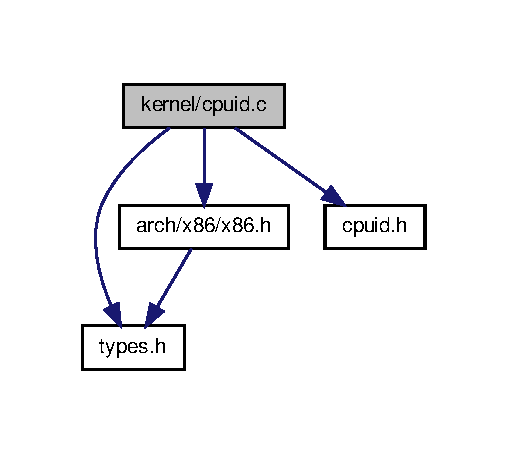
\includegraphics[width=244pt]{cpuid_8c__incl}
\end{center}
\end{figure}
\subsection*{\-Data \-Structures}
\begin{DoxyCompactItemize}
\item 
struct \hyperlink{structcpuid__regs}{cpuid\-\_\-regs}
\end{DoxyCompactItemize}
\subsection*{\-Functions}
\begin{DoxyCompactItemize}
\item 
\hyperlink{types_8h_a435d1572bf3f880d55459d9805097f62}{uint32\-\_\-t} \hyperlink{cpuid_8c_a859ce3c4fd538c7e8259bde51ee95db7}{cpuid\-\_\-get\-\_\-ebx} (void)
\item 
\hyperlink{types_8h_a435d1572bf3f880d55459d9805097f62}{uint32\-\_\-t} \hyperlink{cpuid_8c_afa0d0bb353ccf9cf21b6814977b154ef}{cpuid\-\_\-get\-\_\-ecx} (void)
\item 
\hyperlink{types_8h_a435d1572bf3f880d55459d9805097f62}{uint32\-\_\-t} \hyperlink{cpuid_8c_aa2a5fea9b9bd9993f24373cec6313516}{cpuid\-\_\-get\-\_\-edx} (void)
\item 
\hyperlink{types_8h_a435d1572bf3f880d55459d9805097f62}{uint32\-\_\-t} \hyperlink{cpuid_8c_a86d63e2300f1f529ee483ddd8b18137a}{cpuid\-\_\-get\-\_\-eax} (void)
\item 
static void \hyperlink{cpuid_8c_a3555022a9a455d0783e239690defaf3d}{make\-\_\-cpuid} (\hyperlink{types_8h_a435d1572bf3f880d55459d9805097f62}{uint32\-\_\-t} $\ast$eax, \hyperlink{types_8h_a435d1572bf3f880d55459d9805097f62}{uint32\-\_\-t} $\ast$ebx, \hyperlink{types_8h_a435d1572bf3f880d55459d9805097f62}{uint32\-\_\-t} $\ast$ecx, \hyperlink{types_8h_a435d1572bf3f880d55459d9805097f62}{uint32\-\_\-t} $\ast$edx)
\item 
\hyperlink{types_8h_a435d1572bf3f880d55459d9805097f62}{uint32\-\_\-t} \hyperlink{cpuid_8c_adec7c6888b96c83a0659b36e331ad138}{set\-\_\-eax} (\hyperlink{types_8h_a435d1572bf3f880d55459d9805097f62}{uint32\-\_\-t} value)
\item 
\hyperlink{types_8h_a435d1572bf3f880d55459d9805097f62}{uint32\-\_\-t} \hyperlink{cpuid_8c_a79a861218fed01d656734e810da0229e}{cpuid\-\_\-print} (\hyperlink{types_8h_a435d1572bf3f880d55459d9805097f62}{uint32\-\_\-t} ax\-\_\-value, \hyperlink{types_8h_a435d1572bf3f880d55459d9805097f62}{uint32\-\_\-t} operation)
\end{DoxyCompactItemize}


\subsection{\-Function \-Documentation}
\hypertarget{cpuid_8c_a86d63e2300f1f529ee483ddd8b18137a}{\index{cpuid.\-c@{cpuid.\-c}!cpuid\-\_\-get\-\_\-eax@{cpuid\-\_\-get\-\_\-eax}}
\index{cpuid\-\_\-get\-\_\-eax@{cpuid\-\_\-get\-\_\-eax}!cpuid.c@{cpuid.\-c}}
\subsubsection[{cpuid\-\_\-get\-\_\-eax}]{\setlength{\rightskip}{0pt plus 5cm}{\bf uint32\-\_\-t} {\bf cpuid\-\_\-get\-\_\-eax} (
\begin{DoxyParamCaption}
\item[{void}]{}
\end{DoxyParamCaption}
)}}\label{cpuid_8c_a86d63e2300f1f529ee483ddd8b18137a}
\hypertarget{cpuid_8c_a859ce3c4fd538c7e8259bde51ee95db7}{\index{cpuid.\-c@{cpuid.\-c}!cpuid\-\_\-get\-\_\-ebx@{cpuid\-\_\-get\-\_\-ebx}}
\index{cpuid\-\_\-get\-\_\-ebx@{cpuid\-\_\-get\-\_\-ebx}!cpuid.c@{cpuid.\-c}}
\subsubsection[{cpuid\-\_\-get\-\_\-ebx}]{\setlength{\rightskip}{0pt plus 5cm}{\bf uint32\-\_\-t} {\bf cpuid\-\_\-get\-\_\-ebx} (
\begin{DoxyParamCaption}
\item[{void}]{}
\end{DoxyParamCaption}
)}}\label{cpuid_8c_a859ce3c4fd538c7e8259bde51ee95db7}
\hypertarget{cpuid_8c_afa0d0bb353ccf9cf21b6814977b154ef}{\index{cpuid.\-c@{cpuid.\-c}!cpuid\-\_\-get\-\_\-ecx@{cpuid\-\_\-get\-\_\-ecx}}
\index{cpuid\-\_\-get\-\_\-ecx@{cpuid\-\_\-get\-\_\-ecx}!cpuid.c@{cpuid.\-c}}
\subsubsection[{cpuid\-\_\-get\-\_\-ecx}]{\setlength{\rightskip}{0pt plus 5cm}{\bf uint32\-\_\-t} {\bf cpuid\-\_\-get\-\_\-ecx} (
\begin{DoxyParamCaption}
\item[{void}]{}
\end{DoxyParamCaption}
)}}\label{cpuid_8c_afa0d0bb353ccf9cf21b6814977b154ef}
\hypertarget{cpuid_8c_aa2a5fea9b9bd9993f24373cec6313516}{\index{cpuid.\-c@{cpuid.\-c}!cpuid\-\_\-get\-\_\-edx@{cpuid\-\_\-get\-\_\-edx}}
\index{cpuid\-\_\-get\-\_\-edx@{cpuid\-\_\-get\-\_\-edx}!cpuid.c@{cpuid.\-c}}
\subsubsection[{cpuid\-\_\-get\-\_\-edx}]{\setlength{\rightskip}{0pt plus 5cm}{\bf uint32\-\_\-t} {\bf cpuid\-\_\-get\-\_\-edx} (
\begin{DoxyParamCaption}
\item[{void}]{}
\end{DoxyParamCaption}
)}}\label{cpuid_8c_aa2a5fea9b9bd9993f24373cec6313516}
\hypertarget{cpuid_8c_a79a861218fed01d656734e810da0229e}{\index{cpuid.\-c@{cpuid.\-c}!cpuid\-\_\-print@{cpuid\-\_\-print}}
\index{cpuid\-\_\-print@{cpuid\-\_\-print}!cpuid.c@{cpuid.\-c}}
\subsubsection[{cpuid\-\_\-print}]{\setlength{\rightskip}{0pt plus 5cm}{\bf uint32\-\_\-t} {\bf cpuid\-\_\-print} (
\begin{DoxyParamCaption}
\item[{{\bf uint32\-\_\-t}}]{ax\-\_\-value, }
\item[{{\bf uint32\-\_\-t}}]{operation}
\end{DoxyParamCaption}
)}}\label{cpuid_8c_a79a861218fed01d656734e810da0229e}


\-Definition at line 22 of file cpuid.\-c.

\hypertarget{cpuid_8c_a3555022a9a455d0783e239690defaf3d}{\index{cpuid.\-c@{cpuid.\-c}!make\-\_\-cpuid@{make\-\_\-cpuid}}
\index{make\-\_\-cpuid@{make\-\_\-cpuid}!cpuid.c@{cpuid.\-c}}
\subsubsection[{make\-\_\-cpuid}]{\setlength{\rightskip}{0pt plus 5cm}static void {\bf make\-\_\-cpuid} (
\begin{DoxyParamCaption}
\item[{{\bf uint32\-\_\-t} $\ast$}]{eax, }
\item[{{\bf uint32\-\_\-t} $\ast$}]{ebx, }
\item[{{\bf uint32\-\_\-t} $\ast$}]{ecx, }
\item[{{\bf uint32\-\_\-t} $\ast$}]{edx}
\end{DoxyParamCaption}
)\hspace{0.3cm}{\ttfamily  \mbox{[}inline, static\mbox{]}}}}\label{cpuid_8c_a3555022a9a455d0783e239690defaf3d}


\-Definition at line 45 of file cpuid.\-c.

\hypertarget{cpuid_8c_adec7c6888b96c83a0659b36e331ad138}{\index{cpuid.\-c@{cpuid.\-c}!set\-\_\-eax@{set\-\_\-eax}}
\index{set\-\_\-eax@{set\-\_\-eax}!cpuid.c@{cpuid.\-c}}
\subsubsection[{set\-\_\-eax}]{\setlength{\rightskip}{0pt plus 5cm}{\bf uint32\-\_\-t} {\bf set\-\_\-eax} (
\begin{DoxyParamCaption}
\item[{{\bf uint32\-\_\-t}}]{value}
\end{DoxyParamCaption}
)}}\label{cpuid_8c_adec7c6888b96c83a0659b36e331ad138}


\-Definition at line 18 of file cpuid.\-c.


\hypertarget{init_8c}{\section{kernel/init.c \-File \-Reference}
\label{init_8c}\index{kernel/init.\-c@{kernel/init.\-c}}
}
{\ttfamily \#include $<$types.\-h$>$}\*
{\ttfamily \#include $<$arch/x86/x86.\-h$>$}\*
{\ttfamily \#include $<$memvals.\-h$>$}\*
{\ttfamily \#include $<$string.\-h$>$}\*
{\ttfamily \#include $<$arch/x86/mm/page.\-h$>$}\*
{\ttfamily \#include $<$arch/x86/elf.\-h$>$}\*
{\ttfamily \#include $<$proc/proc.\-h$>$}\*
{\ttfamily \#include $<$init.\-h$>$}\*
\-Include dependency graph for init.\-c\-:\nopagebreak
\begin{figure}[H]
\begin{center}
\leavevmode
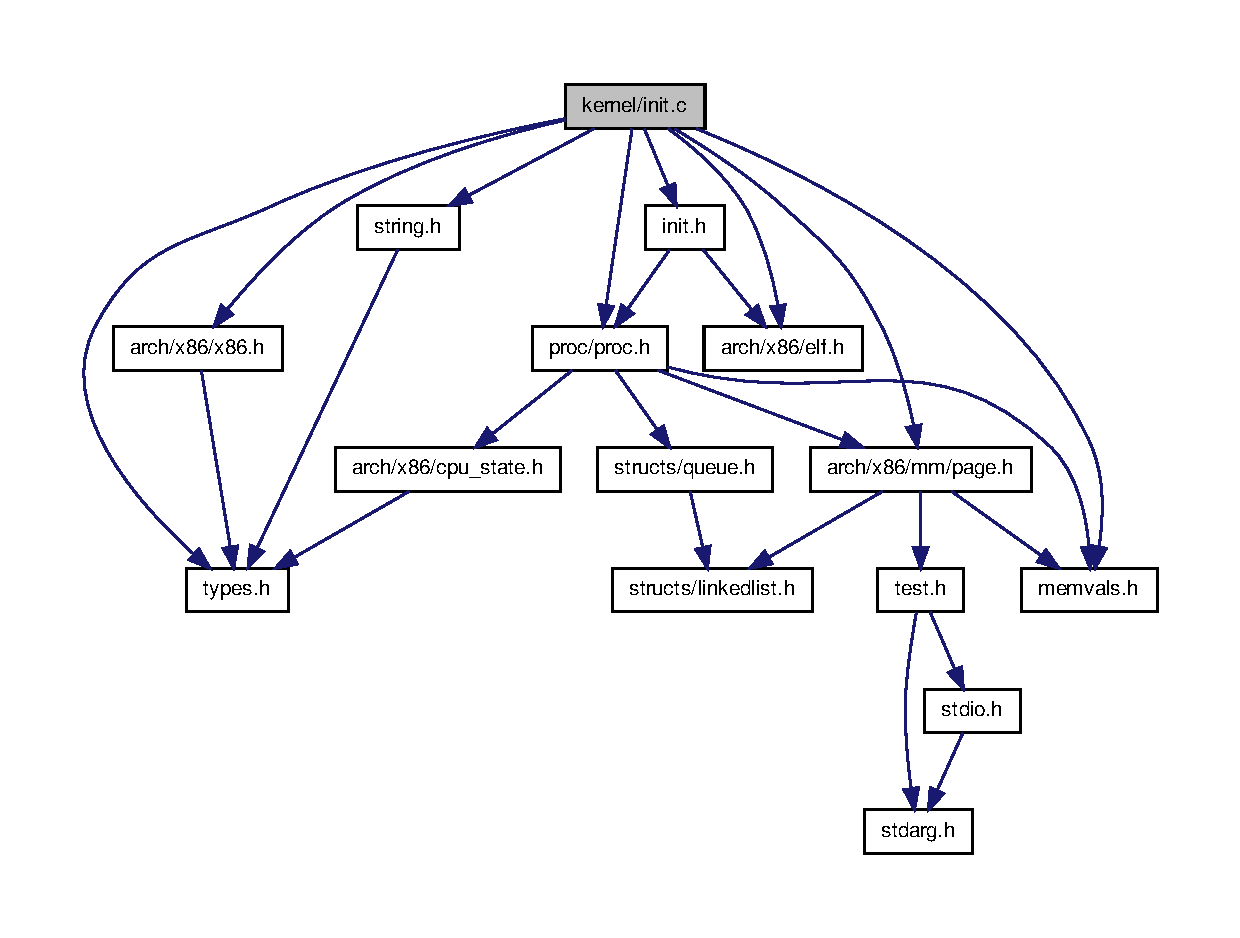
\includegraphics[width=350pt]{init_8c__incl}
\end{center}
\end{figure}
\subsection*{\-Functions}
\begin{DoxyCompactItemize}
\item 
void \hyperlink{init_8c_acb85e8964a153af4bc3a991dcd40906d}{\-Init\-\_\-userspace} (\hyperlink{proc_8h_abcae78bfd085fccd601f7cc568946453}{proc\-\_\-t} $\ast$\hyperlink{structproc}{proc})
\end{DoxyCompactItemize}
\subsection*{\-Variables}
\begin{DoxyCompactItemize}
\item 
\hyperlink{page_8h_a1ae9855ac82633447ab53f25e49e1f62}{pde\-\_\-t} $\ast$ \hyperlink{init_8c_a8ffe8b80013a018b23501ea7a45b7870}{global\-\_\-pgdir}
\item 
struct \hyperlink{structSegdesc}{\-Segdesc} \hyperlink{init_8c_a362a86eab2f1d332cf898b80741c89c9}{catgdt} \mbox{[}$\,$\mbox{]}
\item 
\hyperlink{proc_8h_abcae78bfd085fccd601f7cc568946453}{proc\-\_\-t} \hyperlink{init_8c_a9705bd4b450e5613243c8a63433399c0}{processes} \mbox{[}$\,$\mbox{]}
\end{DoxyCompactItemize}


\subsection{\-Function \-Documentation}
\hypertarget{init_8c_acb85e8964a153af4bc3a991dcd40906d}{\index{init.\-c@{init.\-c}!\-Init\-\_\-userspace@{\-Init\-\_\-userspace}}
\index{\-Init\-\_\-userspace@{\-Init\-\_\-userspace}!init.c@{init.\-c}}
\subsubsection[{\-Init\-\_\-userspace}]{\setlength{\rightskip}{0pt plus 5cm}void {\bf \-Init\-\_\-userspace} (
\begin{DoxyParamCaption}
\item[{{\bf proc\-\_\-t} $\ast$}]{proc}
\end{DoxyParamCaption}
)}}\label{init_8c_acb85e8964a153af4bc3a991dcd40906d}


\-Definition at line 16 of file init.\-c.



\subsection{\-Variable \-Documentation}
\hypertarget{init_8c_a362a86eab2f1d332cf898b80741c89c9}{\index{init.\-c@{init.\-c}!catgdt@{catgdt}}
\index{catgdt@{catgdt}!init.c@{init.\-c}}
\subsubsection[{catgdt}]{\setlength{\rightskip}{0pt plus 5cm}struct {\bf \-Segdesc} {\bf catgdt}\mbox{[}$\,$\mbox{]}}}\label{init_8c_a362a86eab2f1d332cf898b80741c89c9}


\-Definition at line 37 of file init\-\_\-mem.\-c.

\hypertarget{init_8c_a8ffe8b80013a018b23501ea7a45b7870}{\index{init.\-c@{init.\-c}!global\-\_\-pgdir@{global\-\_\-pgdir}}
\index{global\-\_\-pgdir@{global\-\_\-pgdir}!init.c@{init.\-c}}
\subsubsection[{global\-\_\-pgdir}]{\setlength{\rightskip}{0pt plus 5cm}{\bf pde\-\_\-t}$\ast$ {\bf global\-\_\-pgdir}}}\label{init_8c_a8ffe8b80013a018b23501ea7a45b7870}


\-Definition at line 11 of file init.\-c.

\hypertarget{init_8c_a9705bd4b450e5613243c8a63433399c0}{\index{init.\-c@{init.\-c}!processes@{processes}}
\index{processes@{processes}!init.c@{init.\-c}}
\subsubsection[{processes}]{\setlength{\rightskip}{0pt plus 5cm}{\bf proc\-\_\-t} {\bf processes}\mbox{[}$\,$\mbox{]}}}\label{init_8c_a9705bd4b450e5613243c8a63433399c0}

\hypertarget{kbc_8c}{\section{kernel/kbc.c \-File \-Reference}
\label{kbc_8c}\index{kernel/kbc.\-c@{kernel/kbc.\-c}}
}
{\ttfamily \#include $<$types.\-h$>$}\*
{\ttfamily \#include $<$arch/x86/x86.\-h$>$}\*
{\ttfamily \#include $<$cli.\-h$>$}\*
{\ttfamily \#include $<$kbc.\-h$>$}\*
\-Include dependency graph for kbc.\-c\-:\nopagebreak
\begin{figure}[H]
\begin{center}
\leavevmode
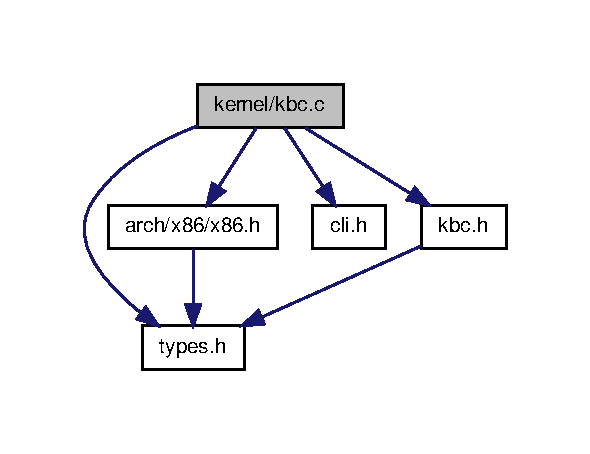
\includegraphics[width=283pt]{kbc_8c__incl}
\end{center}
\end{figure}
\subsection*{\-Defines}
\begin{DoxyCompactItemize}
\item 
\#define \hyperlink{kbc_8c_ad0168eaab1da42b06e86ecf5ff0f6f1d}{\-E\-S\-C\-O\-D\-E}~(1$<$$<$6)
\item 
\#define \hyperlink{kbc_8c_ac16e9c5c93955f2c396aaa9829b72323}{\-C\-T\-L}~(1$<$$<$1)
\item 
\#define \hyperlink{kbc_8c_ac179eef68bcc694aa0ef8dd1eb09950b}{\-S\-H\-I\-F\-T}~(1$<$$<$0)
\item 
\#define \hyperlink{kbc_8c_a9d8a33b1a8b82b9913a0ba70438d45be}{\-A\-L\-T}~(1$<$$<$2)
\item 
\#define \hyperlink{kbc_8c_ad36c01c5d7b1fc13a22426a497ac1b8b}{\-C\-A\-P\-S\-L\-O\-C\-K}~(1$<$$<$3)
\item 
\#define \hyperlink{kbc_8c_a67aa85b3ef56be57b97e084f52621d4f}{\-N\-U\-M\-L\-O\-C\-K}~(1$<$$<$4)
\item 
\#define \hyperlink{kbc_8c_a1cb9c7b41422a2c83136cecfe2a059d3}{\-S\-C\-R\-O\-L\-L\-L\-O\-C\-K}~(1$<$$<$5)
\item 
\#define \hyperlink{kbc_8c_af19d48b9f61047a668649a2f9dc317ff}{\-N\-U\-L}~0
\item 
\#define \hyperlink{kbc_8c_acda3b44286ccc5e1924198027f28a8c5}{\-C\-L}(x)~((x)-\/'@')
\end{DoxyCompactItemize}
\subsection*{\-Functions}
\begin{DoxyCompactItemize}
\item 
int \hyperlink{kbc_8c_aa8584463ac58034ccbf9cd2ffc8e187d}{kbc\-\_\-data} (void)
\item 
void \hyperlink{kbc_8c_abf3ce1c314db9a6a15b99e5313eb2edb}{kbc\-\_\-interrupt} (void)
\end{DoxyCompactItemize}
\subsection*{\-Variables}
\begin{DoxyCompactItemize}
\item 
static \hyperlink{types_8h_aba7bc1797add20fe3efdf37ced1182c5}{uint8\-\_\-t} \hyperlink{kbc_8c_a4326db5874cbf6cc212076fab5d49976}{shiftcode} \mbox{[}256\mbox{]}
\item 
static \hyperlink{types_8h_aba7bc1797add20fe3efdf37ced1182c5}{uint8\-\_\-t} \hyperlink{kbc_8c_a04894af8115f470aa8f26efdde3b6742}{togglecode} \mbox{[}256\mbox{]}
\item 
static \hyperlink{types_8h_aba7bc1797add20fe3efdf37ced1182c5}{uint8\-\_\-t} \hyperlink{kbc_8c_aecaf43d20653affe9dcc677b2cab809d}{normalmap} \mbox{[}256\mbox{]}
\item 
static \hyperlink{types_8h_aba7bc1797add20fe3efdf37ced1182c5}{uint8\-\_\-t} \hyperlink{kbc_8c_a7d97552a829d8810a5914cc12c325052}{shiftmap} \mbox{[}256\mbox{]}
\item 
static \hyperlink{types_8h_aba7bc1797add20fe3efdf37ced1182c5}{uint8\-\_\-t} \hyperlink{kbc_8c_a9fcaddcec928a650c8414586b7f42265}{ctlmap} \mbox{[}256\mbox{]}
\item 
static \hyperlink{types_8h_aba7bc1797add20fe3efdf37ced1182c5}{uint8\-\_\-t} $\ast$ \hyperlink{kbc_8c_a0a67bc2d04dda86f0eebaabad58355d8}{charcode} \mbox{[}4\mbox{]}
\end{DoxyCompactItemize}


\subsection{\-Define \-Documentation}
\hypertarget{kbc_8c_a9d8a33b1a8b82b9913a0ba70438d45be}{\index{kbc.\-c@{kbc.\-c}!\-A\-L\-T@{\-A\-L\-T}}
\index{\-A\-L\-T@{\-A\-L\-T}!kbc.c@{kbc.\-c}}
\subsubsection[{\-A\-L\-T}]{\setlength{\rightskip}{0pt plus 5cm}\#define {\bf \-A\-L\-T}~(1$<$$<$2)}}\label{kbc_8c_a9d8a33b1a8b82b9913a0ba70438d45be}


\-Definition at line 11 of file kbc.\-c.

\hypertarget{kbc_8c_ad36c01c5d7b1fc13a22426a497ac1b8b}{\index{kbc.\-c@{kbc.\-c}!\-C\-A\-P\-S\-L\-O\-C\-K@{\-C\-A\-P\-S\-L\-O\-C\-K}}
\index{\-C\-A\-P\-S\-L\-O\-C\-K@{\-C\-A\-P\-S\-L\-O\-C\-K}!kbc.c@{kbc.\-c}}
\subsubsection[{\-C\-A\-P\-S\-L\-O\-C\-K}]{\setlength{\rightskip}{0pt plus 5cm}\#define {\bf \-C\-A\-P\-S\-L\-O\-C\-K}~(1$<$$<$3)}}\label{kbc_8c_ad36c01c5d7b1fc13a22426a497ac1b8b}


\-Definition at line 12 of file kbc.\-c.

\hypertarget{kbc_8c_acda3b44286ccc5e1924198027f28a8c5}{\index{kbc.\-c@{kbc.\-c}!\-C\-L@{\-C\-L}}
\index{\-C\-L@{\-C\-L}!kbc.c@{kbc.\-c}}
\subsubsection[{\-C\-L}]{\setlength{\rightskip}{0pt plus 5cm}\#define {\bf \-C\-L}(
\begin{DoxyParamCaption}
\item[{}]{x}
\end{DoxyParamCaption}
)~((x)-\/'@')}}\label{kbc_8c_acda3b44286ccc5e1924198027f28a8c5}


\-Definition at line 72 of file kbc.\-c.

\hypertarget{kbc_8c_ac16e9c5c93955f2c396aaa9829b72323}{\index{kbc.\-c@{kbc.\-c}!\-C\-T\-L@{\-C\-T\-L}}
\index{\-C\-T\-L@{\-C\-T\-L}!kbc.c@{kbc.\-c}}
\subsubsection[{\-C\-T\-L}]{\setlength{\rightskip}{0pt plus 5cm}\#define {\bf \-C\-T\-L}~(1$<$$<$1)}}\label{kbc_8c_ac16e9c5c93955f2c396aaa9829b72323}


\-Definition at line 9 of file kbc.\-c.

\hypertarget{kbc_8c_ad0168eaab1da42b06e86ecf5ff0f6f1d}{\index{kbc.\-c@{kbc.\-c}!\-E\-S\-C\-O\-D\-E@{\-E\-S\-C\-O\-D\-E}}
\index{\-E\-S\-C\-O\-D\-E@{\-E\-S\-C\-O\-D\-E}!kbc.c@{kbc.\-c}}
\subsubsection[{\-E\-S\-C\-O\-D\-E}]{\setlength{\rightskip}{0pt plus 5cm}\#define {\bf \-E\-S\-C\-O\-D\-E}~(1$<$$<$6)}}\label{kbc_8c_ad0168eaab1da42b06e86ecf5ff0f6f1d}


\-Definition at line 8 of file kbc.\-c.

\hypertarget{kbc_8c_af19d48b9f61047a668649a2f9dc317ff}{\index{kbc.\-c@{kbc.\-c}!\-N\-U\-L@{\-N\-U\-L}}
\index{\-N\-U\-L@{\-N\-U\-L}!kbc.c@{kbc.\-c}}
\subsubsection[{\-N\-U\-L}]{\setlength{\rightskip}{0pt plus 5cm}\#define {\bf \-N\-U\-L}~0}}\label{kbc_8c_af19d48b9f61047a668649a2f9dc317ff}


\-Definition at line 31 of file kbc.\-c.

\hypertarget{kbc_8c_a67aa85b3ef56be57b97e084f52621d4f}{\index{kbc.\-c@{kbc.\-c}!\-N\-U\-M\-L\-O\-C\-K@{\-N\-U\-M\-L\-O\-C\-K}}
\index{\-N\-U\-M\-L\-O\-C\-K@{\-N\-U\-M\-L\-O\-C\-K}!kbc.c@{kbc.\-c}}
\subsubsection[{\-N\-U\-M\-L\-O\-C\-K}]{\setlength{\rightskip}{0pt plus 5cm}\#define {\bf \-N\-U\-M\-L\-O\-C\-K}~(1$<$$<$4)}}\label{kbc_8c_a67aa85b3ef56be57b97e084f52621d4f}


\-Definition at line 13 of file kbc.\-c.

\hypertarget{kbc_8c_a1cb9c7b41422a2c83136cecfe2a059d3}{\index{kbc.\-c@{kbc.\-c}!\-S\-C\-R\-O\-L\-L\-L\-O\-C\-K@{\-S\-C\-R\-O\-L\-L\-L\-O\-C\-K}}
\index{\-S\-C\-R\-O\-L\-L\-L\-O\-C\-K@{\-S\-C\-R\-O\-L\-L\-L\-O\-C\-K}!kbc.c@{kbc.\-c}}
\subsubsection[{\-S\-C\-R\-O\-L\-L\-L\-O\-C\-K}]{\setlength{\rightskip}{0pt plus 5cm}\#define {\bf \-S\-C\-R\-O\-L\-L\-L\-O\-C\-K}~(1$<$$<$5)}}\label{kbc_8c_a1cb9c7b41422a2c83136cecfe2a059d3}


\-Definition at line 14 of file kbc.\-c.

\hypertarget{kbc_8c_ac179eef68bcc694aa0ef8dd1eb09950b}{\index{kbc.\-c@{kbc.\-c}!\-S\-H\-I\-F\-T@{\-S\-H\-I\-F\-T}}
\index{\-S\-H\-I\-F\-T@{\-S\-H\-I\-F\-T}!kbc.c@{kbc.\-c}}
\subsubsection[{\-S\-H\-I\-F\-T}]{\setlength{\rightskip}{0pt plus 5cm}\#define {\bf \-S\-H\-I\-F\-T}~(1$<$$<$0)}}\label{kbc_8c_ac179eef68bcc694aa0ef8dd1eb09950b}


\-Definition at line 10 of file kbc.\-c.



\subsection{\-Function \-Documentation}
\hypertarget{kbc_8c_aa8584463ac58034ccbf9cd2ffc8e187d}{\index{kbc.\-c@{kbc.\-c}!kbc\-\_\-data@{kbc\-\_\-data}}
\index{kbc\-\_\-data@{kbc\-\_\-data}!kbc.c@{kbc.\-c}}
\subsubsection[{kbc\-\_\-data}]{\setlength{\rightskip}{0pt plus 5cm}int {\bf kbc\-\_\-data} (
\begin{DoxyParamCaption}
\item[{void}]{}
\end{DoxyParamCaption}
)}}\label{kbc_8c_aa8584463ac58034ccbf9cd2ffc8e187d}


\-Definition at line 97 of file kbc.\-c.

\hypertarget{kbc_8c_abf3ce1c314db9a6a15b99e5313eb2edb}{\index{kbc.\-c@{kbc.\-c}!kbc\-\_\-interrupt@{kbc\-\_\-interrupt}}
\index{kbc\-\_\-interrupt@{kbc\-\_\-interrupt}!kbc.c@{kbc.\-c}}
\subsubsection[{kbc\-\_\-interrupt}]{\setlength{\rightskip}{0pt plus 5cm}void {\bf kbc\-\_\-interrupt} (
\begin{DoxyParamCaption}
\item[{void}]{}
\end{DoxyParamCaption}
)}}\label{kbc_8c_abf3ce1c314db9a6a15b99e5313eb2edb}


\-Definition at line 131 of file kbc.\-c.



\subsection{\-Variable \-Documentation}
\hypertarget{kbc_8c_a0a67bc2d04dda86f0eebaabad58355d8}{\index{kbc.\-c@{kbc.\-c}!charcode@{charcode}}
\index{charcode@{charcode}!kbc.c@{kbc.\-c}}
\subsubsection[{charcode}]{\setlength{\rightskip}{0pt plus 5cm}{\bf uint8\-\_\-t}$\ast$ {\bf charcode}\mbox{[}4\mbox{]}\hspace{0.3cm}{\ttfamily  \mbox{[}static\mbox{]}}}}\label{kbc_8c_a0a67bc2d04dda86f0eebaabad58355d8}
{\bfseries \-Initial value\-:}
\begin{DoxyCode}
 {
        normalmap,
        shiftmap,
        ctlmap,
        ctlmap
}
\end{DoxyCode}


\-Definition at line 91 of file kbc.\-c.

\hypertarget{kbc_8c_a9fcaddcec928a650c8414586b7f42265}{\index{kbc.\-c@{kbc.\-c}!ctlmap@{ctlmap}}
\index{ctlmap@{ctlmap}!kbc.c@{kbc.\-c}}
\subsubsection[{ctlmap}]{\setlength{\rightskip}{0pt plus 5cm}{\bf uint8\-\_\-t} {\bf ctlmap}\mbox{[}256\mbox{]}\hspace{0.3cm}{\ttfamily  \mbox{[}static\mbox{]}}}}\label{kbc_8c_a9fcaddcec928a650c8414586b7f42265}
{\bfseries \-Initial value\-:}
\begin{DoxyCode}

{
        NUL,    NUL,    NUL,    NUL,    NUL,    NUL,    NUL,    NUL,
        NUL,    NUL,    NUL,    NUL,    NUL,    NUL,    NUL,    NUL,
        CL('Q'),CL('W'),CL('E'),CL('R'),CL('T'),CL('Y'),CL('U'),CL('I'),
        CL('O'),CL('P'),NUL,    NUL,    '\r',   NUL,    CL('A'),CL('S'),
        CL('D'),CL('F'),CL('G'),CL('H'),CL('J'),CL('K'),CL('L'),NUL,
        NUL,    NUL,    NUL,    CL('\\'),CL('Z'),CL('X'),CL('C'),CL('V'),
        CL('B'),CL('N'),CL('M'),NUL,    NUL,    CL('/'),NUL,    NUL,
        [0x97] KEY_HOME,        [0x9C] '\n',
        [0xB5] CL('/'),         [0xC8] KEY_UP,
        [0xC9] KEY_PGUP,        [0xCB] KEY_LF,
        [0xCD] KEY_RT,          [0xCF] KEY_END,
        [0xD0] KEY_DN,          [0xD1] KEY_PGDN,
        [0xD2] KEY_INS,         [0xD3] KEY_DEL


}
\end{DoxyCode}


\-Definition at line 73 of file kbc.\-c.

\hypertarget{kbc_8c_aecaf43d20653affe9dcc677b2cab809d}{\index{kbc.\-c@{kbc.\-c}!normalmap@{normalmap}}
\index{normalmap@{normalmap}!kbc.c@{kbc.\-c}}
\subsubsection[{normalmap}]{\setlength{\rightskip}{0pt plus 5cm}{\bf uint8\-\_\-t} {\bf normalmap}\mbox{[}256\mbox{]}\hspace{0.3cm}{\ttfamily  \mbox{[}static\mbox{]}}}}\label{kbc_8c_aecaf43d20653affe9dcc677b2cab809d}
{\bfseries \-Initial value\-:}
\begin{DoxyCode}

{
        NUL,0x1B,'1','2','3','4','5','6',
        '7','8','9','0','-','=','\b','\t',
        'q','w','e','r','t','y','u','i',
        'o','p','[',']','\n',NUL,'a','s',
        'd','f','g','h','j','k','l',';',
        '\'','`',NUL,'\\','z','x','c',
        'v','b','n','m',',','.','/',NUL,'*',
        NUL,' ',NUL,NUL,NUL,NUL,NUL,NUL,NUL,
        NUL,NUL,NUL,NUL,NUL,NUL,'7','8','9',
        '-','4','5','6','+','1','2','3','0',
        '.', NUL, NUL, NUL, NUL,
        [0x97] KEY_HOME,        [0x9C] '\n',
        [0xB5] '/',             [0xC8] KEY_UP,
        [0xC9] KEY_PGUP,        [0xCB] KEY_LF,
        [0xCD] KEY_RT,          [0xCF] KEY_END,
        [0xD0] KEY_DN,          [0xD1] KEY_PGDN,
        [0xD2] KEY_INS,         [0xD3] KEY_DEL
}
\end{DoxyCode}


\-Definition at line 32 of file kbc.\-c.

\hypertarget{kbc_8c_a4326db5874cbf6cc212076fab5d49976}{\index{kbc.\-c@{kbc.\-c}!shiftcode@{shiftcode}}
\index{shiftcode@{shiftcode}!kbc.c@{kbc.\-c}}
\subsubsection[{shiftcode}]{\setlength{\rightskip}{0pt plus 5cm}{\bf uint8\-\_\-t} {\bf shiftcode}\mbox{[}256\mbox{]}\hspace{0.3cm}{\ttfamily  \mbox{[}static\mbox{]}}}}\label{kbc_8c_a4326db5874cbf6cc212076fab5d49976}
{\bfseries \-Initial value\-:}
\begin{DoxyCode}

{
        [0x1D] CTL,
        [0x2A] SHIFT,
        [0x36] SHIFT,
        [0x38] ALT,
        [0x9D] CTL,
        [0xB8] ALT

}
\end{DoxyCode}


\-Definition at line 15 of file kbc.\-c.

\hypertarget{kbc_8c_a7d97552a829d8810a5914cc12c325052}{\index{kbc.\-c@{kbc.\-c}!shiftmap@{shiftmap}}
\index{shiftmap@{shiftmap}!kbc.c@{kbc.\-c}}
\subsubsection[{shiftmap}]{\setlength{\rightskip}{0pt plus 5cm}{\bf uint8\-\_\-t} {\bf shiftmap}\mbox{[}256\mbox{]}\hspace{0.3cm}{\ttfamily  \mbox{[}static\mbox{]}}}}\label{kbc_8c_a7d97552a829d8810a5914cc12c325052}
{\bfseries \-Initial value\-:}
\begin{DoxyCode}

{
        NUL,0x1B,'!','@','#','$','%','^',
        '&','*','(',')','_','+','\b','\t',
        'Q','W','E','R','T','Y','U','I','O',
        'P','{','}','\n',NUL,'A','S','D','F',
        'G','H','J','K','L',':','"','~',
        NUL,'|','Z','X','C','V','B','N','M',
        '<','>','?',NUL,'*',NUL,' ',NUL,NUL,
        NUL,NUL,NUL,NUL,NUL,NUL,NUL,NUL,NUL,
        NUL,NUL,'7','8','9','-','4','5','6',
        '+','1','2','3','0','.', NUL,NUL,NUL,NUL,
        [0x97] KEY_HOME,        [0x9C] '\n',
        [0xB5] '/',             [0xC8] KEY_UP,
        [0xC9] KEY_PGUP,        [0xCB] KEY_LF,
        [0xCD] KEY_RT,          [0xCF] KEY_END,
        [0xD0] KEY_DN,          [0xD1] KEY_PGDN,
        [0xD2] KEY_INS,         [0xD3] KEY_DEL
}
\end{DoxyCode}


\-Definition at line 53 of file kbc.\-c.

\hypertarget{kbc_8c_a04894af8115f470aa8f26efdde3b6742}{\index{kbc.\-c@{kbc.\-c}!togglecode@{togglecode}}
\index{togglecode@{togglecode}!kbc.c@{kbc.\-c}}
\subsubsection[{togglecode}]{\setlength{\rightskip}{0pt plus 5cm}{\bf uint8\-\_\-t} {\bf togglecode}\mbox{[}256\mbox{]}\hspace{0.3cm}{\ttfamily  \mbox{[}static\mbox{]}}}}\label{kbc_8c_a04894af8115f470aa8f26efdde3b6742}
{\bfseries \-Initial value\-:}
\begin{DoxyCode}

{
        [0x3A] CAPSLOCK,
        [0x45] NUMLOCK,
        [0x46] SCROLLLOCK
}
\end{DoxyCode}


\-Definition at line 25 of file kbc.\-c.


\hypertarget{play_8c}{\section{kernel/play.c \-File \-Reference}
\label{play_8c}\index{kernel/play.\-c@{kernel/play.\-c}}
}


kernel main file  


{\ttfamily \#include $<$types.\-h$>$}\*
{\ttfamily \#include $<$cli.\-h$>$}\*
{\ttfamily \#include $<$stdio.\-h$>$}\*
{\ttfamily \#include $<$video.\-h$>$}\*
{\ttfamily \#include $<$cmos.\-h$>$}\*
{\ttfamily \#include $<$arch/x86/x86.\-h$>$}\*
{\ttfamily \#include $<$cpuid.\-h$>$}\*
{\ttfamily \#include $<$proc/proc.\-h$>$}\*
{\ttfamily \#include $<$test.\-h$>$}\*
\-Include dependency graph for play.\-c\-:\nopagebreak
\begin{figure}[H]
\begin{center}
\leavevmode
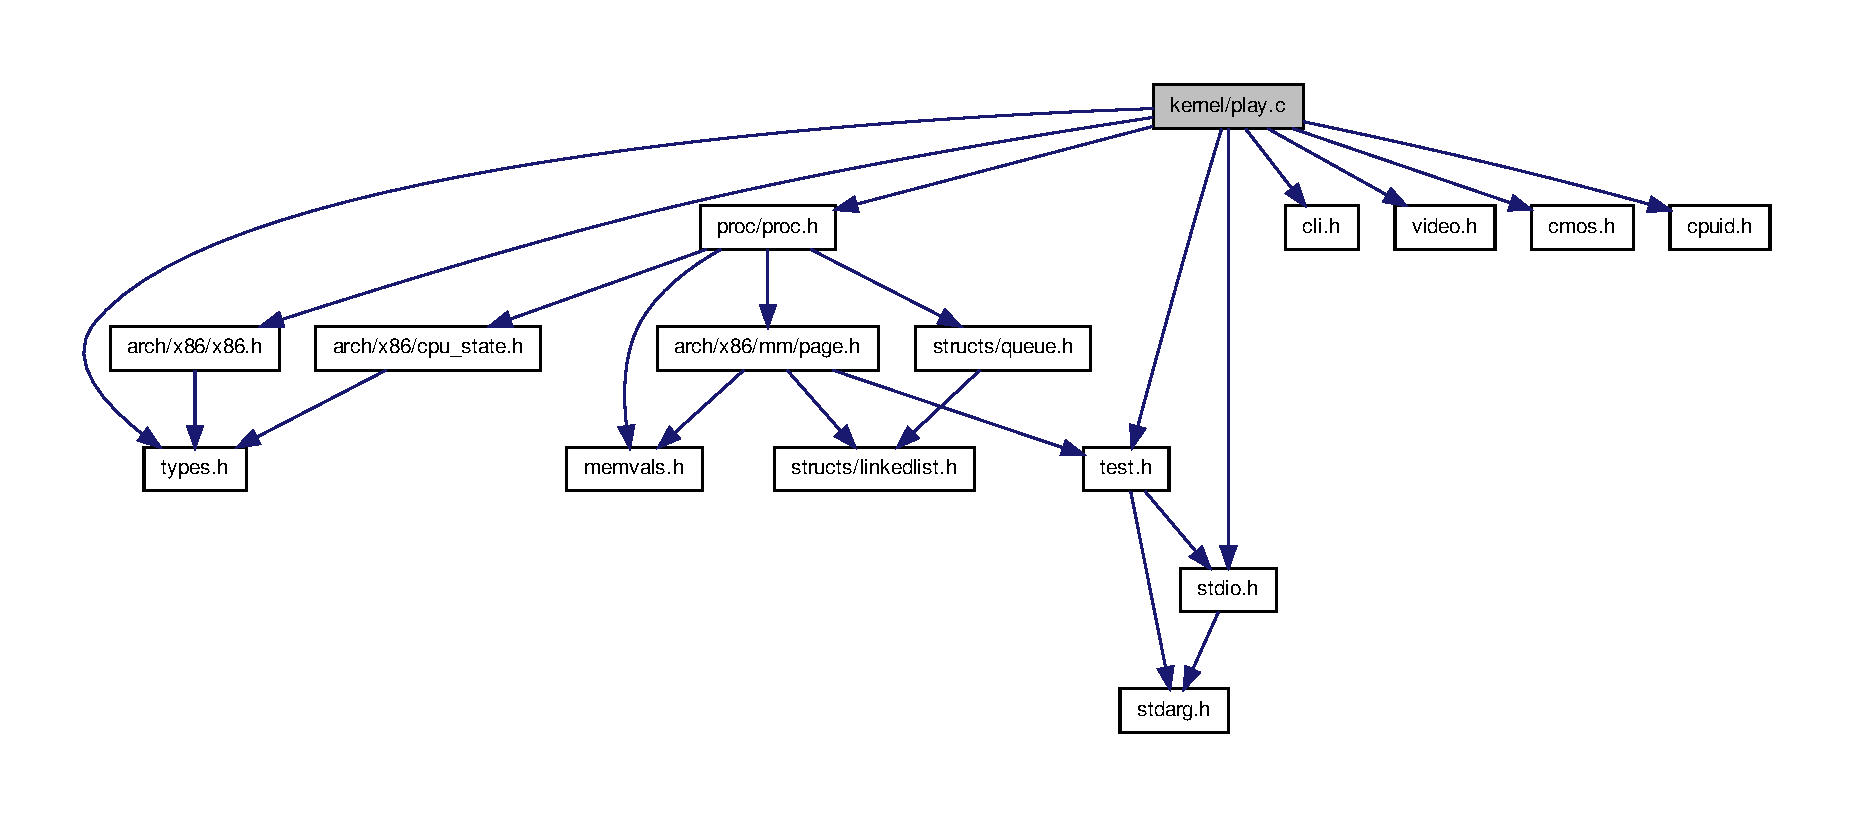
\includegraphics[width=350pt]{play_8c__incl}
\end{center}
\end{figure}
\subsection*{\-Functions}
\begin{DoxyCompactItemize}
\item 
void \hyperlink{group__main_gabdfb298c4eb2fba465cab1235f1c3723}{play} (void)
\item 
void \hyperlink{group__main_gaa3af12553c8338d80c22e90f5e12c1e1}{\-\_\-panic\-\_\-} (const char $\ast$file, int nline, const char $\ast$fmt,...)
\item 
void \hyperlink{group__main_ga380ccbaccf8fe8f6927022cf0ce4384f}{time\-\_\-print} (void)
\item 
void \hyperlink{group__main_ga7510f52822177f82d8b2bcb8e88b7939}{bootup} (void)
\end{DoxyCompactItemize}
\subsection*{\-Variables}
\begin{DoxyCompactItemize}
\item 
static const char $\ast$ \hyperlink{group__main_ga242a1c3e4fc9ceac904f34981d990d35}{error\-\_\-panic} = \hyperlink{types_8h_a070d2ce7b6bb7e5c05602aa8c308d0c4}{\-N\-U\-L\-L}
\end{DoxyCompactItemize}


\subsection{\-Detailed \-Description}
kernel main file \-Saad \-Talaat \begin{DoxyDate}{\-Date}
12/9/2011 \-Description goes here 
\end{DoxyDate}


\-Definition in file \hyperlink{}{play.\-c}.


\hypertarget{printf_8c}{\section{kernel/printf.c \-File \-Reference}
\label{printf_8c}\index{kernel/printf.\-c@{kernel/printf.\-c}}
}
{\ttfamily \#include $<$types.\-h$>$}\*
{\ttfamily \#include $<$stdio.\-h$>$}\*
\-Include dependency graph for printf.\-c\-:\nopagebreak
\begin{figure}[H]
\begin{center}
\leavevmode
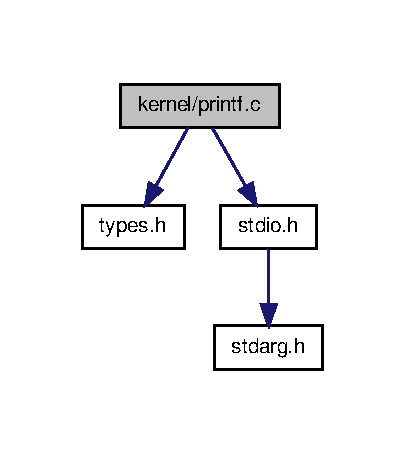
\includegraphics[width=195pt]{printf_8c__incl}
\end{center}
\end{figure}
\subsection*{\-Defines}
\begin{DoxyCompactItemize}
\item 
\#define \hyperlink{printf_8c_a4d22860a6ae6b1a2fc3b6c1f44af59a8}{hex2ascii}(x)~(\char`\"{}0123456789\-A\-B\-C\-D\-E\-F\char`\"{}\mbox{[}x\mbox{]})
\end{DoxyCompactItemize}
\subsection*{\-Functions}
\begin{DoxyCompactItemize}
\item 
static void \hyperlink{printf_8c_a2c0f7b90b6771c3ac60fcba2da990672}{putch} (int c, int $\ast$count)
\item 
void \hyperlink{printf_8c_a4d96a0e0fd1a548e704a5408d77c33cb}{ksprintkn} (void($\ast$func)(int, int $\ast$), int $\ast$count, \hyperlink{types_8h_a2ba5f6c0633401558d277b2c0e4f758d}{uintmax\-\_\-t} num, int \hyperlink{memvals_8h_a0523cedff47e2441fc198b7770ec5d3f}{base}, int width, int padc)
\item 
int \hyperlink{printf_8c_a15fa6d5bac62e4e23535055899f8198a}{getint} (\hyperlink{stdarg_8h_abaefbc6cabb217bf0138d4f9c94d4775}{va\-\_\-list} $\ast$ap, int lflag)
\item 
int \hyperlink{printf_8c_aa2d6b6655726ec3ed608623a0fa2efc5}{getuint} (\hyperlink{stdarg_8h_abaefbc6cabb217bf0138d4f9c94d4775}{va\-\_\-list} $\ast$ap, int lflag)
\item 
int \hyperlink{printf_8c_a39a5e13b8f9ef35f6878c6dc086d3463}{kvprintk} (const char $\ast$format, void($\ast$func)(int, int $\ast$), int $\ast$count, \hyperlink{stdarg_8h_abaefbc6cabb217bf0138d4f9c94d4775}{va\-\_\-list} ap)
\item 
\hyperlink{printf_8c_a1965a44d004e945de8e4a662cdfac402}{vprintk} (const char $\ast$format, \hyperlink{stdarg_8h_abaefbc6cabb217bf0138d4f9c94d4775}{va\-\_\-list} ap)
\item 
int \hyperlink{printf_8c_a36fe4a3ea4506cb4d128b11f93187f71}{printk} (const char $\ast$format,...)
\end{DoxyCompactItemize}


\subsection{\-Define \-Documentation}
\hypertarget{printf_8c_a4d22860a6ae6b1a2fc3b6c1f44af59a8}{\index{printf.\-c@{printf.\-c}!hex2ascii@{hex2ascii}}
\index{hex2ascii@{hex2ascii}!printf.c@{printf.\-c}}
\subsubsection[{hex2ascii}]{\setlength{\rightskip}{0pt plus 5cm}\#define {\bf hex2ascii}(
\begin{DoxyParamCaption}
\item[{}]{x}
\end{DoxyParamCaption}
)~(\char`\"{}0123456789\-A\-B\-C\-D\-E\-F\char`\"{}\mbox{[}x\mbox{]})}}\label{printf_8c_a4d22860a6ae6b1a2fc3b6c1f44af59a8}


\-Definition at line 4 of file printf.\-c.



\subsection{\-Function \-Documentation}
\hypertarget{printf_8c_a15fa6d5bac62e4e23535055899f8198a}{\index{printf.\-c@{printf.\-c}!getint@{getint}}
\index{getint@{getint}!printf.c@{printf.\-c}}
\subsubsection[{getint}]{\setlength{\rightskip}{0pt plus 5cm}int {\bf getint} (
\begin{DoxyParamCaption}
\item[{{\bf va\-\_\-list} $\ast$}]{ap, }
\item[{int}]{lflag}
\end{DoxyParamCaption}
)}}\label{printf_8c_a15fa6d5bac62e4e23535055899f8198a}


\-Definition at line 21 of file printf.\-c.

\hypertarget{printf_8c_aa2d6b6655726ec3ed608623a0fa2efc5}{\index{printf.\-c@{printf.\-c}!getuint@{getuint}}
\index{getuint@{getuint}!printf.c@{printf.\-c}}
\subsubsection[{getuint}]{\setlength{\rightskip}{0pt plus 5cm}int {\bf getuint} (
\begin{DoxyParamCaption}
\item[{{\bf va\-\_\-list} $\ast$}]{ap, }
\item[{int}]{lflag}
\end{DoxyParamCaption}
)}}\label{printf_8c_aa2d6b6655726ec3ed608623a0fa2efc5}


\-Definition at line 31 of file printf.\-c.

\hypertarget{printf_8c_a4d96a0e0fd1a548e704a5408d77c33cb}{\index{printf.\-c@{printf.\-c}!ksprintkn@{ksprintkn}}
\index{ksprintkn@{ksprintkn}!printf.c@{printf.\-c}}
\subsubsection[{ksprintkn}]{\setlength{\rightskip}{0pt plus 5cm}void {\bf ksprintkn} (
\begin{DoxyParamCaption}
\item[{void($\ast$)(int, int $\ast$)}]{func, }
\item[{int $\ast$}]{count, }
\item[{{\bf uintmax\-\_\-t}}]{num, }
\item[{int}]{base, }
\item[{int}]{width, }
\item[{int}]{padc}
\end{DoxyParamCaption}
)}}\label{printf_8c_a4d96a0e0fd1a548e704a5408d77c33cb}


\-Definition at line 10 of file printf.\-c.

\hypertarget{printf_8c_a39a5e13b8f9ef35f6878c6dc086d3463}{\index{printf.\-c@{printf.\-c}!kvprintk@{kvprintk}}
\index{kvprintk@{kvprintk}!printf.c@{printf.\-c}}
\subsubsection[{kvprintk}]{\setlength{\rightskip}{0pt plus 5cm}int {\bf kvprintk} (
\begin{DoxyParamCaption}
\item[{const char $\ast$}]{format, }
\item[{void($\ast$)(int, int $\ast$)}]{func, }
\item[{int $\ast$}]{count, }
\item[{{\bf va\-\_\-list}}]{ap}
\end{DoxyParamCaption}
)}}\label{printf_8c_a39a5e13b8f9ef35f6878c6dc086d3463}


\-Definition at line 43 of file printf.\-c.

\hypertarget{printf_8c_a36fe4a3ea4506cb4d128b11f93187f71}{\index{printf.\-c@{printf.\-c}!printk@{printk}}
\index{printk@{printk}!printf.c@{printf.\-c}}
\subsubsection[{printk}]{\setlength{\rightskip}{0pt plus 5cm}int {\bf printk} (
\begin{DoxyParamCaption}
\item[{const char $\ast$}]{format, }
\item[{}]{...}
\end{DoxyParamCaption}
)}}\label{printf_8c_a36fe4a3ea4506cb4d128b11f93187f71}


\-Definition at line 167 of file printf.\-c.

\hypertarget{printf_8c_a2c0f7b90b6771c3ac60fcba2da990672}{\index{printf.\-c@{printf.\-c}!putch@{putch}}
\index{putch@{putch}!printf.c@{printf.\-c}}
\subsubsection[{putch}]{\setlength{\rightskip}{0pt plus 5cm}static void {\bf putch} (
\begin{DoxyParamCaption}
\item[{int}]{c, }
\item[{int $\ast$}]{count}
\end{DoxyParamCaption}
)\hspace{0.3cm}{\ttfamily  \mbox{[}static\mbox{]}}}}\label{printf_8c_a2c0f7b90b6771c3ac60fcba2da990672}


\-Definition at line 6 of file printf.\-c.

\hypertarget{printf_8c_a1965a44d004e945de8e4a662cdfac402}{\index{printf.\-c@{printf.\-c}!vprintk@{vprintk}}
\index{vprintk@{vprintk}!printf.c@{printf.\-c}}
\subsubsection[{vprintk}]{\setlength{\rightskip}{0pt plus 5cm}{\bf vprintk} (
\begin{DoxyParamCaption}
\item[{const char $\ast$}]{format, }
\item[{{\bf va\-\_\-list}}]{ap}
\end{DoxyParamCaption}
)}}\label{printf_8c_a1965a44d004e945de8e4a662cdfac402}


\-Definition at line 160 of file printf.\-c.


\hypertarget{load__elf_8c}{\section{kernel/proc/load\-\_\-elf.c \-File \-Reference}
\label{load__elf_8c}\index{kernel/proc/load\-\_\-elf.\-c@{kernel/proc/load\-\_\-elf.\-c}}
}
{\ttfamily \#include $<$types.\-h$>$}\*
{\ttfamily \#include $<$arch/x86/elf.\-h$>$}\*
{\ttfamily \#include $<$memvals.\-h$>$}\*
{\ttfamily \#include $<$proc/proc.\-h$>$}\*
{\ttfamily \#include $<$rdisk.\-h$>$}\*
\-Include dependency graph for load\-\_\-elf.\-c\-:\nopagebreak
\begin{figure}[H]
\begin{center}
\leavevmode
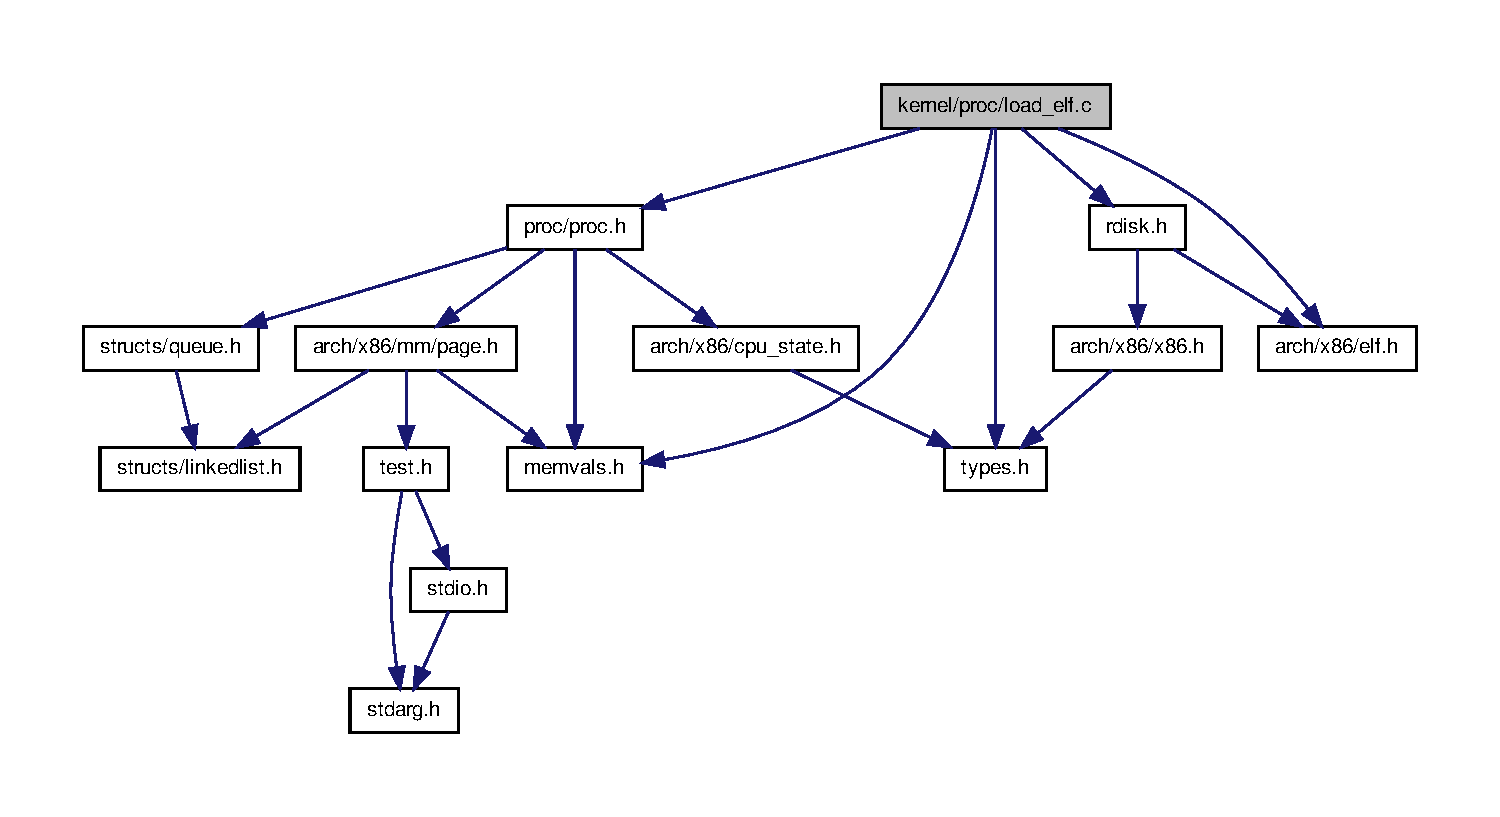
\includegraphics[width=350pt]{load__elf_8c__incl}
\end{center}
\end{figure}
\subsection*{\-Functions}
\begin{DoxyCompactItemize}
\item 
\hyperlink{types_8h_a435d1572bf3f880d55459d9805097f62}{uint32\-\_\-t} \hyperlink{load__elf_8c_a2672ea9e3b3140f2a7861de2a4372aa2}{elf\-\_\-load\-\_\-to\-\_\-proc} (\hyperlink{proc_8h_abcae78bfd085fccd601f7cc568946453}{proc\-\_\-t} $\ast$\hyperlink{structproc}{proc}, \hyperlink{types_8h_a435d1572bf3f880d55459d9805097f62}{uint32\-\_\-t} offset)
\end{DoxyCompactItemize}


\subsection{\-Function \-Documentation}
\hypertarget{load__elf_8c_a2672ea9e3b3140f2a7861de2a4372aa2}{\index{load\-\_\-elf.\-c@{load\-\_\-elf.\-c}!elf\-\_\-load\-\_\-to\-\_\-proc@{elf\-\_\-load\-\_\-to\-\_\-proc}}
\index{elf\-\_\-load\-\_\-to\-\_\-proc@{elf\-\_\-load\-\_\-to\-\_\-proc}!load_elf.c@{load\-\_\-elf.\-c}}
\subsubsection[{elf\-\_\-load\-\_\-to\-\_\-proc}]{\setlength{\rightskip}{0pt plus 5cm}{\bf uint32\-\_\-t} {\bf elf\-\_\-load\-\_\-to\-\_\-proc} (
\begin{DoxyParamCaption}
\item[{{\bf proc\-\_\-t} $\ast$}]{proc, }
\item[{{\bf uint32\-\_\-t}}]{offset}
\end{DoxyParamCaption}
)}}\label{load__elf_8c_a2672ea9e3b3140f2a7861de2a4372aa2}


\-Definition at line 8 of file load\-\_\-elf.\-c.


\hypertarget{proc_8c}{\section{kernel/proc/proc.c \-File \-Reference}
\label{proc_8c}\index{kernel/proc/proc.\-c@{kernel/proc/proc.\-c}}
}
{\ttfamily \#include $<$types.\-h$>$}\*
{\ttfamily \#include $<$memvals.\-h$>$}\*
{\ttfamily \#include $<$proc/proc.\-h$>$}\*
{\ttfamily \#include $<$arch/x86/mm/segdesc.\-h$>$}\*
{\ttfamily \#include $<$arch/x86/processor.\-h$>$}\*
{\ttfamily \#include $<$string.\-h$>$}\*
{\ttfamily \#include $<$init.\-h$>$}\*
{\ttfamily \#include $<$rdisk.\-h$>$}\*
\-Include dependency graph for proc.\-c\-:\nopagebreak
\begin{figure}[H]
\begin{center}
\leavevmode
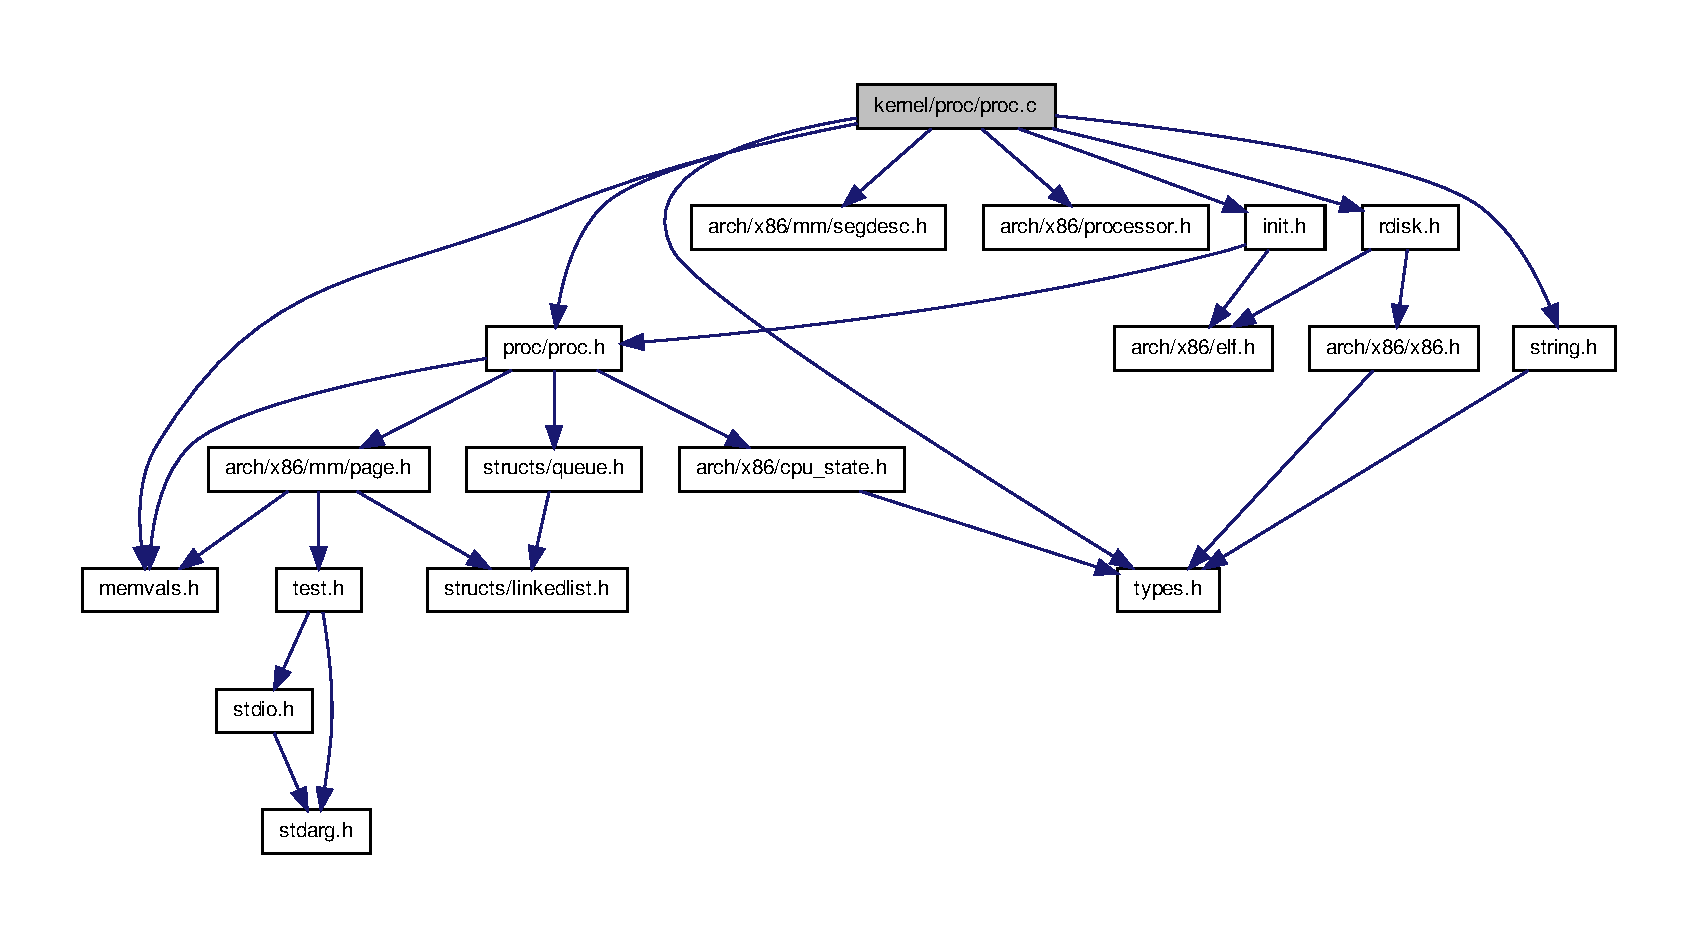
\includegraphics[width=350pt]{proc_8c__incl}
\end{center}
\end{figure}
\subsection*{\-Functions}
\begin{DoxyCompactItemize}
\item 
void \hyperlink{proc_8c_a7a86f136018ec12ba764d8ecc13ee403}{init\-\_\-proc\-\_\-table} (void)
\item 
\hyperlink{types_8h_a435d1572bf3f880d55459d9805097f62}{uint32\-\_\-t} \hyperlink{proc_8c_af9b0729d454bfcd1cccac25668e1cdd5}{create\-\_\-proc} (\hyperlink{proc_8h_abcae78bfd085fccd601f7cc568946453}{proc\-\_\-t} $\ast$$\ast$proc\-\_\-s)
\item 
\hyperlink{types_8h_a435d1572bf3f880d55459d9805097f62}{uint32\-\_\-t} \hyperlink{proc_8c_a068b8a94b58e77fc6cf65795fd0b5aac}{proc\-\_\-alloc\-\_\-mem} (\hyperlink{proc_8h_abcae78bfd085fccd601f7cc568946453}{proc\-\_\-t} $\ast$\hyperlink{structproc}{proc}, void $\ast$va, \hyperlink{types_8h_a435d1572bf3f880d55459d9805097f62}{uint32\-\_\-t} len)
\item 
\hyperlink{types_8h_a435d1572bf3f880d55459d9805097f62}{uint32\-\_\-t} \hyperlink{proc_8c_ae6e0fd99b6fae7f9b0c5575193151d58}{init\-\_\-proc0} ()
\item 
void \hyperlink{proc_8c_a3adc819d4b6f54184f72a00e0584190f}{init\-\_\-proc} (void)
\item 
void \hyperlink{proc_8c_a5786a19c8d7e97d107ad3e1c02c12b0d}{test\-\_\-lifo} (void)
\item 
void \hyperlink{proc_8c_a34033e3a55f39ca55025d33eb49aa313}{switch\-\_\-address\-\_\-space} (\hyperlink{proc_8h_abcae78bfd085fccd601f7cc568946453}{proc\-\_\-t} $\ast$proc\-\_\-to\-\_\-run)
\end{DoxyCompactItemize}
\subsection*{\-Variables}
\begin{DoxyCompactItemize}
\item 
\hyperlink{page_8h_a1ae9855ac82633447ab53f25e49e1f62}{pde\-\_\-t} $\ast$ \hyperlink{proc_8c_a8ffe8b80013a018b23501ea7a45b7870}{global\-\_\-pgdir}
\item 
struct \-Proc\-\_\-\-List \hyperlink{proc_8c_a10d7952b0ace8f68027e672286c44b33}{empty\-\_\-procs}
\item 
\hyperlink{proc_8h_abcae78bfd085fccd601f7cc568946453}{proc\-\_\-t} $\ast$ \hyperlink{proc_8c_a432b7b292b7d2423daf04aceac8924e6}{proc\-\_\-table}
\item 
struct \-Proc\-\_\-\-Lifo \hyperlink{proc_8c_a7608dc18b85a71c7c6f32b45a8516d12}{running\-\_\-procs}
\end{DoxyCompactItemize}


\subsection{\-Function \-Documentation}
\hypertarget{proc_8c_af9b0729d454bfcd1cccac25668e1cdd5}{\index{proc.\-c@{proc.\-c}!create\-\_\-proc@{create\-\_\-proc}}
\index{create\-\_\-proc@{create\-\_\-proc}!proc.c@{proc.\-c}}
\subsubsection[{create\-\_\-proc}]{\setlength{\rightskip}{0pt plus 5cm}{\bf uint32\-\_\-t} {\bf create\-\_\-proc} (
\begin{DoxyParamCaption}
\item[{{\bf proc\-\_\-t} $\ast$$\ast$}]{proc\-\_\-s}
\end{DoxyParamCaption}
)}}\label{proc_8c_af9b0729d454bfcd1cccac25668e1cdd5}


\-Definition at line 56 of file proc.\-c.

\hypertarget{proc_8c_a3adc819d4b6f54184f72a00e0584190f}{\index{proc.\-c@{proc.\-c}!init\-\_\-proc@{init\-\_\-proc}}
\index{init\-\_\-proc@{init\-\_\-proc}!proc.c@{proc.\-c}}
\subsubsection[{init\-\_\-proc}]{\setlength{\rightskip}{0pt plus 5cm}void {\bf init\-\_\-proc} (
\begin{DoxyParamCaption}
\item[{void}]{}
\end{DoxyParamCaption}
)}}\label{proc_8c_a3adc819d4b6f54184f72a00e0584190f}


\-Definition at line 112 of file proc.\-c.

\hypertarget{proc_8c_ae6e0fd99b6fae7f9b0c5575193151d58}{\index{proc.\-c@{proc.\-c}!init\-\_\-proc0@{init\-\_\-proc0}}
\index{init\-\_\-proc0@{init\-\_\-proc0}!proc.c@{proc.\-c}}
\subsubsection[{init\-\_\-proc0}]{\setlength{\rightskip}{0pt plus 5cm}{\bf uint32\-\_\-t} {\bf init\-\_\-proc0} (
\begin{DoxyParamCaption}
{}
\end{DoxyParamCaption}
)}}\label{proc_8c_ae6e0fd99b6fae7f9b0c5575193151d58}


\-Definition at line 101 of file proc.\-c.

\hypertarget{proc_8c_a7a86f136018ec12ba764d8ecc13ee403}{\index{proc.\-c@{proc.\-c}!init\-\_\-proc\-\_\-table@{init\-\_\-proc\-\_\-table}}
\index{init\-\_\-proc\-\_\-table@{init\-\_\-proc\-\_\-table}!proc.c@{proc.\-c}}
\subsubsection[{init\-\_\-proc\-\_\-table}]{\setlength{\rightskip}{0pt plus 5cm}void {\bf init\-\_\-proc\-\_\-table} (
\begin{DoxyParamCaption}
\item[{void}]{}
\end{DoxyParamCaption}
)}}\label{proc_8c_a7a86f136018ec12ba764d8ecc13ee403}


\-Definition at line 17 of file proc.\-c.

\hypertarget{proc_8c_a068b8a94b58e77fc6cf65795fd0b5aac}{\index{proc.\-c@{proc.\-c}!proc\-\_\-alloc\-\_\-mem@{proc\-\_\-alloc\-\_\-mem}}
\index{proc\-\_\-alloc\-\_\-mem@{proc\-\_\-alloc\-\_\-mem}!proc.c@{proc.\-c}}
\subsubsection[{proc\-\_\-alloc\-\_\-mem}]{\setlength{\rightskip}{0pt plus 5cm}{\bf uint32\-\_\-t} {\bf proc\-\_\-alloc\-\_\-mem} (
\begin{DoxyParamCaption}
\item[{{\bf proc\-\_\-t} $\ast$}]{proc, }
\item[{void $\ast$}]{va, }
\item[{{\bf uint32\-\_\-t}}]{len}
\end{DoxyParamCaption}
)}}\label{proc_8c_a068b8a94b58e77fc6cf65795fd0b5aac}


\-Definition at line 84 of file proc.\-c.

\hypertarget{proc_8c_a34033e3a55f39ca55025d33eb49aa313}{\index{proc.\-c@{proc.\-c}!switch\-\_\-address\-\_\-space@{switch\-\_\-address\-\_\-space}}
\index{switch\-\_\-address\-\_\-space@{switch\-\_\-address\-\_\-space}!proc.c@{proc.\-c}}
\subsubsection[{switch\-\_\-address\-\_\-space}]{\setlength{\rightskip}{0pt plus 5cm}void {\bf switch\-\_\-address\-\_\-space} (
\begin{DoxyParamCaption}
\item[{{\bf proc\-\_\-t} $\ast$}]{proc\-\_\-to\-\_\-run}
\end{DoxyParamCaption}
)}}\label{proc_8c_a34033e3a55f39ca55025d33eb49aa313}


\-Definition at line 138 of file proc.\-c.

\hypertarget{proc_8c_a5786a19c8d7e97d107ad3e1c02c12b0d}{\index{proc.\-c@{proc.\-c}!test\-\_\-lifo@{test\-\_\-lifo}}
\index{test\-\_\-lifo@{test\-\_\-lifo}!proc.c@{proc.\-c}}
\subsubsection[{test\-\_\-lifo}]{\setlength{\rightskip}{0pt plus 5cm}void {\bf test\-\_\-lifo} (
\begin{DoxyParamCaption}
\item[{void}]{}
\end{DoxyParamCaption}
)}}\label{proc_8c_a5786a19c8d7e97d107ad3e1c02c12b0d}


\-Definition at line 119 of file proc.\-c.



\subsection{\-Variable \-Documentation}
\hypertarget{proc_8c_a10d7952b0ace8f68027e672286c44b33}{\index{proc.\-c@{proc.\-c}!empty\-\_\-procs@{empty\-\_\-procs}}
\index{empty\-\_\-procs@{empty\-\_\-procs}!proc.c@{proc.\-c}}
\subsubsection[{empty\-\_\-procs}]{\setlength{\rightskip}{0pt plus 5cm}struct \-Proc\-\_\-\-List {\bf empty\-\_\-procs}}}\label{proc_8c_a10d7952b0ace8f68027e672286c44b33}


\-Definition at line 11 of file proc.\-c.

\hypertarget{proc_8c_a8ffe8b80013a018b23501ea7a45b7870}{\index{proc.\-c@{proc.\-c}!global\-\_\-pgdir@{global\-\_\-pgdir}}
\index{global\-\_\-pgdir@{global\-\_\-pgdir}!proc.c@{proc.\-c}}
\subsubsection[{global\-\_\-pgdir}]{\setlength{\rightskip}{0pt plus 5cm}{\bf pde\-\_\-t}$\ast$ {\bf global\-\_\-pgdir}}}\label{proc_8c_a8ffe8b80013a018b23501ea7a45b7870}


\-Definition at line 13 of file page.\-c.

\hypertarget{proc_8c_a432b7b292b7d2423daf04aceac8924e6}{\index{proc.\-c@{proc.\-c}!proc\-\_\-table@{proc\-\_\-table}}
\index{proc\-\_\-table@{proc\-\_\-table}!proc.c@{proc.\-c}}
\subsubsection[{proc\-\_\-table}]{\setlength{\rightskip}{0pt plus 5cm}{\bf proc\-\_\-t}$\ast$ {\bf proc\-\_\-table}}}\label{proc_8c_a432b7b292b7d2423daf04aceac8924e6}


\-Definition at line 13 of file proc.\-c.

\hypertarget{proc_8c_a7608dc18b85a71c7c6f32b45a8516d12}{\index{proc.\-c@{proc.\-c}!running\-\_\-procs@{running\-\_\-procs}}
\index{running\-\_\-procs@{running\-\_\-procs}!proc.c@{proc.\-c}}
\subsubsection[{running\-\_\-procs}]{\setlength{\rightskip}{0pt plus 5cm}struct \-Proc\-\_\-\-Lifo {\bf running\-\_\-procs}}}\label{proc_8c_a7608dc18b85a71c7c6f32b45a8516d12}


\-Definition at line 14 of file proc.\-c.


\hypertarget{rdisk_8c}{\section{kernel/rdisk.c \-File \-Reference}
\label{rdisk_8c}\index{kernel/rdisk.\-c@{kernel/rdisk.\-c}}
}
{\ttfamily \#include $<$rdisk.\-h$>$}\*
{\ttfamily \#include $<$arch/x86/x86.\-h$>$}\*
{\ttfamily \#include $<$arch/x86/elf.\-h$>$}\*
\-Include dependency graph for rdisk.\-c\-:\nopagebreak
\begin{figure}[H]
\begin{center}
\leavevmode
\includegraphics[width=257pt]{rdisk_8c__incl}
\end{center}
\end{figure}
\subsection*{\-Functions}
\begin{DoxyCompactItemize}
\item 
void \hyperlink{rdisk_8c_a8bc2062a175b7c74607a2498ac997657}{readsect} (void $\ast$, \hyperlink{types_8h_a435d1572bf3f880d55459d9805097f62}{uint32\-\_\-t})
\item 
void \hyperlink{rdisk_8c_a687601dc22e8d4d8407608c91fd325eb}{readseg} (\hyperlink{types_8h_a435d1572bf3f880d55459d9805097f62}{uint32\-\_\-t}, \hyperlink{types_8h_a435d1572bf3f880d55459d9805097f62}{uint32\-\_\-t}, \hyperlink{types_8h_a435d1572bf3f880d55459d9805097f62}{uint32\-\_\-t})
\item 
void \hyperlink{rdisk_8c_a63222d4a07c38c198de5bd116a001935}{waitdisk} (void)
\end{DoxyCompactItemize}


\subsection{\-Function \-Documentation}
\hypertarget{rdisk_8c_a8bc2062a175b7c74607a2498ac997657}{\index{rdisk.\-c@{rdisk.\-c}!readsect@{readsect}}
\index{readsect@{readsect}!rdisk.c@{rdisk.\-c}}
\subsubsection[{readsect}]{\setlength{\rightskip}{0pt plus 5cm}void {\bf readsect} (
\begin{DoxyParamCaption}
\item[{void $\ast$}]{dst, }
\item[{{\bf uint32\-\_\-t}}]{offset}
\end{DoxyParamCaption}
)}}\label{rdisk_8c_a8bc2062a175b7c74607a2498ac997657}


\-Definition at line 36 of file rdisk.\-c.

\hypertarget{rdisk_8c_a687601dc22e8d4d8407608c91fd325eb}{\index{rdisk.\-c@{rdisk.\-c}!readseg@{readseg}}
\index{readseg@{readseg}!rdisk.c@{rdisk.\-c}}
\subsubsection[{readseg}]{\setlength{\rightskip}{0pt plus 5cm}void {\bf readseg} (
\begin{DoxyParamCaption}
\item[{{\bf uint32\-\_\-t}}]{va, }
\item[{{\bf uint32\-\_\-t}}]{count, }
\item[{{\bf uint32\-\_\-t}}]{offset}
\end{DoxyParamCaption}
)}}\label{rdisk_8c_a687601dc22e8d4d8407608c91fd325eb}


\-Definition at line 11 of file rdisk.\-c.

\hypertarget{rdisk_8c_a63222d4a07c38c198de5bd116a001935}{\index{rdisk.\-c@{rdisk.\-c}!waitdisk@{waitdisk}}
\index{waitdisk@{waitdisk}!rdisk.c@{rdisk.\-c}}
\subsubsection[{waitdisk}]{\setlength{\rightskip}{0pt plus 5cm}void {\bf waitdisk} (
\begin{DoxyParamCaption}
\item[{void}]{}
\end{DoxyParamCaption}
)}}\label{rdisk_8c_a63222d4a07c38c198de5bd116a001935}


\-Definition at line 57 of file rdisk.\-c.


\hypertarget{readline_8c}{\section{kernel/readline.c \-File \-Reference}
\label{readline_8c}\index{kernel/readline.\-c@{kernel/readline.\-c}}
}
{\ttfamily \#include $<$types.\-h$>$}\*
{\ttfamily \#include $<$kbc.\-h$>$}\*
{\ttfamily \#include $<$stdio.\-h$>$}\*
{\ttfamily \#include $<$video.\-h$>$}\*
\-Include dependency graph for readline.\-c\-:\nopagebreak
\begin{figure}[H]
\begin{center}
\leavevmode
\includegraphics[width=282pt]{readline_8c__incl}
\end{center}
\end{figure}
\subsection*{\-Defines}
\begin{DoxyCompactItemize}
\item 
\#define \hyperlink{readline_8c_ad974fe981249f5e84fbf1683b012c9f8}{\-B\-U\-F\-L\-E\-N}~1024
\end{DoxyCompactItemize}
\subsection*{\-Functions}
\begin{DoxyCompactItemize}
\item 
char $\ast$ \hyperlink{readline_8c_a2d8df50da224fdc6607a12e71c22f86b}{readline} (const char $\ast$towrite)
\end{DoxyCompactItemize}
\subsection*{\-Variables}
\begin{DoxyCompactItemize}
\item 
static char \hyperlink{readline_8c_a397f08d200458b6bf4ff83cf31325bfa}{buf} \mbox{[}\hyperlink{readline_8c_ad974fe981249f5e84fbf1683b012c9f8}{\-B\-U\-F\-L\-E\-N}\mbox{]}
\end{DoxyCompactItemize}


\subsection{\-Define \-Documentation}
\hypertarget{readline_8c_ad974fe981249f5e84fbf1683b012c9f8}{\index{readline.\-c@{readline.\-c}!\-B\-U\-F\-L\-E\-N@{\-B\-U\-F\-L\-E\-N}}
\index{\-B\-U\-F\-L\-E\-N@{\-B\-U\-F\-L\-E\-N}!readline.c@{readline.\-c}}
\subsubsection[{\-B\-U\-F\-L\-E\-N}]{\setlength{\rightskip}{0pt plus 5cm}\#define {\bf \-B\-U\-F\-L\-E\-N}~1024}}\label{readline_8c_ad974fe981249f5e84fbf1683b012c9f8}


\-Definition at line 6 of file readline.\-c.



\subsection{\-Function \-Documentation}
\hypertarget{readline_8c_a2d8df50da224fdc6607a12e71c22f86b}{\index{readline.\-c@{readline.\-c}!readline@{readline}}
\index{readline@{readline}!readline.c@{readline.\-c}}
\subsubsection[{readline}]{\setlength{\rightskip}{0pt plus 5cm}char$\ast$ {\bf readline} (
\begin{DoxyParamCaption}
\item[{const char $\ast$}]{towrite}
\end{DoxyParamCaption}
)}}\label{readline_8c_a2d8df50da224fdc6607a12e71c22f86b}


\-Definition at line 10 of file readline.\-c.



\subsection{\-Variable \-Documentation}
\hypertarget{readline_8c_a397f08d200458b6bf4ff83cf31325bfa}{\index{readline.\-c@{readline.\-c}!buf@{buf}}
\index{buf@{buf}!readline.c@{readline.\-c}}
\subsubsection[{buf}]{\setlength{\rightskip}{0pt plus 5cm}char {\bf buf}\mbox{[}{\bf \-B\-U\-F\-L\-E\-N}\mbox{]}\hspace{0.3cm}{\ttfamily  \mbox{[}static\mbox{]}}}}\label{readline_8c_a397f08d200458b6bf4ff83cf31325bfa}


\-Definition at line 7 of file readline.\-c.


\hypertarget{string_8c}{\section{kernel/string.c \-File \-Reference}
\label{string_8c}\index{kernel/string.\-c@{kernel/string.\-c}}
}
{\ttfamily \#include $<$string.\-h$>$}\*
\-Include dependency graph for string.\-c\-:\nopagebreak
\begin{figure}[H]
\begin{center}
\leavevmode
\includegraphics[width=158pt]{string_8c__incl}
\end{center}
\end{figure}
\subsection*{\-Functions}
\begin{DoxyCompactItemize}
\item 
\hyperlink{types_8h_a435d1572bf3f880d55459d9805097f62}{uint32\-\_\-t} \hyperlink{string_8c_a2e7b2907250be8edc8e78f5dc91cd85b}{strnlen} (const char $\ast$str, \hyperlink{types_8h_a435d1572bf3f880d55459d9805097f62}{uint32\-\_\-t} count)
\item 
void $\ast$ \hyperlink{string_8c_a5beb6f763ff14a288fbe9c1f526579a3}{memcopy} (void $\ast$dst, const void $\ast$src, \hyperlink{types_8h_a435d1572bf3f880d55459d9805097f62}{uint32\-\_\-t} count)
\item 
void $\ast$ \hyperlink{string_8c_aed8d67a6c62c63e36f1f8e071188bdfe}{memset} (void $\ast$ptr, int c, \hyperlink{types_8h_a435d1572bf3f880d55459d9805097f62}{uint32\-\_\-t} count)
\end{DoxyCompactItemize}


\subsection{\-Function \-Documentation}
\hypertarget{string_8c_a5beb6f763ff14a288fbe9c1f526579a3}{\index{string.\-c@{string.\-c}!memcopy@{memcopy}}
\index{memcopy@{memcopy}!string.c@{string.\-c}}
\subsubsection[{memcopy}]{\setlength{\rightskip}{0pt plus 5cm}void$\ast$ {\bf memcopy} (
\begin{DoxyParamCaption}
\item[{void $\ast$}]{dst, }
\item[{const void $\ast$}]{src, }
\item[{{\bf uint32\-\_\-t}}]{count}
\end{DoxyParamCaption}
)}}\label{string_8c_a5beb6f763ff14a288fbe9c1f526579a3}


\-Definition at line 12 of file string.\-c.

\hypertarget{string_8c_aed8d67a6c62c63e36f1f8e071188bdfe}{\index{string.\-c@{string.\-c}!memset@{memset}}
\index{memset@{memset}!string.c@{string.\-c}}
\subsubsection[{memset}]{\setlength{\rightskip}{0pt plus 5cm}void$\ast$ {\bf memset} (
\begin{DoxyParamCaption}
\item[{void $\ast$}]{ptr, }
\item[{int}]{c, }
\item[{{\bf uint32\-\_\-t}}]{count}
\end{DoxyParamCaption}
)}}\label{string_8c_aed8d67a6c62c63e36f1f8e071188bdfe}


\-Definition at line 24 of file string.\-c.

\hypertarget{string_8c_a2e7b2907250be8edc8e78f5dc91cd85b}{\index{string.\-c@{string.\-c}!strnlen@{strnlen}}
\index{strnlen@{strnlen}!string.c@{string.\-c}}
\subsubsection[{strnlen}]{\setlength{\rightskip}{0pt plus 5cm}{\bf uint32\-\_\-t} {\bf strnlen} (
\begin{DoxyParamCaption}
\item[{const char $\ast$}]{str, }
\item[{{\bf uint32\-\_\-t}}]{count}
\end{DoxyParamCaption}
)}}\label{string_8c_a2e7b2907250be8edc8e78f5dc91cd85b}


\-Definition at line 4 of file string.\-c.


\hypertarget{init__elf_8c}{\section{kernel/tmp/init\-\_\-elf.c \-File \-Reference}
\label{init__elf_8c}\index{kernel/tmp/init\-\_\-elf.\-c@{kernel/tmp/init\-\_\-elf.\-c}}
}
\subsection*{\-Functions}
\begin{DoxyCompactItemize}
\item 
int \hyperlink{init__elf_8c_a840291bc02cba5474a4cb46a9b9566fe}{main} (void)
\end{DoxyCompactItemize}


\subsection{\-Function \-Documentation}
\hypertarget{init__elf_8c_a840291bc02cba5474a4cb46a9b9566fe}{\index{init\-\_\-elf.\-c@{init\-\_\-elf.\-c}!main@{main}}
\index{main@{main}!init_elf.c@{init\-\_\-elf.\-c}}
\subsubsection[{main}]{\setlength{\rightskip}{0pt plus 5cm}int {\bf main} (
\begin{DoxyParamCaption}
\item[{void}]{}
\end{DoxyParamCaption}
)}}\label{init__elf_8c_a840291bc02cba5474a4cb46a9b9566fe}


\-Definition at line 3 of file init\-\_\-elf.\-c.


\hypertarget{video_8c}{\section{kernel/video.c \-File \-Reference}
\label{video_8c}\index{kernel/video.\-c@{kernel/video.\-c}}
}
{\ttfamily \#include $<$arch/x86/x86.\-h$>$}\*
{\ttfamily \#include $<$types.\-h$>$}\*
{\ttfamily \#include $<$video.\-h$>$}\*
{\ttfamily \#include $<$memvals.\-h$>$}\*
{\ttfamily \#include $<$kbc.\-h$>$}\*
\-Include dependency graph for video.\-c\-:\nopagebreak
\begin{figure}[H]
\begin{center}
\leavevmode
\includegraphics[width=350pt]{video_8c__incl}
\end{center}
\end{figure}
\subsection*{\-Functions}
\begin{DoxyCompactItemize}
\item 
\hyperlink{types_8h_a273cf69d639a59973b6019625df33e30}{uint16\-\_\-t} \hyperlink{video_8c_a395d60b7d3454851db53889826e8d72e}{cga\-\_\-get\-\_\-pos} (void)
\item 
void \hyperlink{video_8c_a5ab3d2356d4335b222e739300a6dbcb6}{cga\-\_\-set\-\_\-attr} (\hyperlink{types_8h_a273cf69d639a59973b6019625df33e30}{uint16\-\_\-t} c)
\item 
void \hyperlink{video_8c_a2ac77fae84030fe22301c6cdb918bfdb}{cga\-\_\-clear} (void)
\item 
void \hyperlink{video_8c_a98e2b5ab9f34fc634a00c8ac89200b2e}{cga\-\_\-set\-\_\-pos} (\hyperlink{types_8h_a273cf69d639a59973b6019625df33e30}{uint16\-\_\-t} pos)
\item 
void \hyperlink{video_8c_ab0ab5e709ff4fc4d57b7007cd4e305be}{cga\-\_\-init} (void)
\item 
void \hyperlink{video_8c_aca189a8fb5d14a6ccaabfb4ce606e20c}{cga\-\_\-putc} (int c)
\item 
\hyperlink{video_8c_aa52715a04e18ce4c3392ac12b39631f5}{cga\-\_\-putstr} (char $\ast$c)
\end{DoxyCompactItemize}
\subsection*{\-Variables}
\begin{DoxyCompactItemize}
\item 
static \hyperlink{video_8c_a26a60f0654a4abc3c6f3ad02c83601e2}{cga\-\_\-attr}
\end{DoxyCompactItemize}


\subsection{\-Function \-Documentation}
\hypertarget{video_8c_a2ac77fae84030fe22301c6cdb918bfdb}{\index{video.\-c@{video.\-c}!cga\-\_\-clear@{cga\-\_\-clear}}
\index{cga\-\_\-clear@{cga\-\_\-clear}!video.c@{video.\-c}}
\subsubsection[{cga\-\_\-clear}]{\setlength{\rightskip}{0pt plus 5cm}void {\bf cga\-\_\-clear} (
\begin{DoxyParamCaption}
\item[{void}]{}
\end{DoxyParamCaption}
)}}\label{video_8c_a2ac77fae84030fe22301c6cdb918bfdb}


\-Definition at line 31 of file video.\-c.

\hypertarget{video_8c_a395d60b7d3454851db53889826e8d72e}{\index{video.\-c@{video.\-c}!cga\-\_\-get\-\_\-pos@{cga\-\_\-get\-\_\-pos}}
\index{cga\-\_\-get\-\_\-pos@{cga\-\_\-get\-\_\-pos}!video.c@{video.\-c}}
\subsubsection[{cga\-\_\-get\-\_\-pos}]{\setlength{\rightskip}{0pt plus 5cm}{\bf uint16\-\_\-t} {\bf cga\-\_\-get\-\_\-pos} (
\begin{DoxyParamCaption}
\item[{void}]{}
\end{DoxyParamCaption}
)}}\label{video_8c_a395d60b7d3454851db53889826e8d72e}


\-Definition at line 18 of file video.\-c.

\hypertarget{video_8c_ab0ab5e709ff4fc4d57b7007cd4e305be}{\index{video.\-c@{video.\-c}!cga\-\_\-init@{cga\-\_\-init}}
\index{cga\-\_\-init@{cga\-\_\-init}!video.c@{video.\-c}}
\subsubsection[{cga\-\_\-init}]{\setlength{\rightskip}{0pt plus 5cm}void {\bf cga\-\_\-init} (
\begin{DoxyParamCaption}
\item[{void}]{}
\end{DoxyParamCaption}
)}}\label{video_8c_ab0ab5e709ff4fc4d57b7007cd4e305be}


\-Definition at line 48 of file video.\-c.

\hypertarget{video_8c_aca189a8fb5d14a6ccaabfb4ce606e20c}{\index{video.\-c@{video.\-c}!cga\-\_\-putc@{cga\-\_\-putc}}
\index{cga\-\_\-putc@{cga\-\_\-putc}!video.c@{video.\-c}}
\subsubsection[{cga\-\_\-putc}]{\setlength{\rightskip}{0pt plus 5cm}void {\bf cga\-\_\-putc} (
\begin{DoxyParamCaption}
\item[{int}]{c}
\end{DoxyParamCaption}
)}}\label{video_8c_aca189a8fb5d14a6ccaabfb4ce606e20c}


\-Definition at line 59 of file video.\-c.

\hypertarget{video_8c_aa52715a04e18ce4c3392ac12b39631f5}{\index{video.\-c@{video.\-c}!cga\-\_\-putstr@{cga\-\_\-putstr}}
\index{cga\-\_\-putstr@{cga\-\_\-putstr}!video.c@{video.\-c}}
\subsubsection[{cga\-\_\-putstr}]{\setlength{\rightskip}{0pt plus 5cm}{\bf cga\-\_\-putstr} (
\begin{DoxyParamCaption}
\item[{char $\ast$}]{c}
\end{DoxyParamCaption}
)}}\label{video_8c_aa52715a04e18ce4c3392ac12b39631f5}


\-Definition at line 107 of file video.\-c.

\hypertarget{video_8c_a5ab3d2356d4335b222e739300a6dbcb6}{\index{video.\-c@{video.\-c}!cga\-\_\-set\-\_\-attr@{cga\-\_\-set\-\_\-attr}}
\index{cga\-\_\-set\-\_\-attr@{cga\-\_\-set\-\_\-attr}!video.c@{video.\-c}}
\subsubsection[{cga\-\_\-set\-\_\-attr}]{\setlength{\rightskip}{0pt plus 5cm}void {\bf cga\-\_\-set\-\_\-attr} (
\begin{DoxyParamCaption}
\item[{{\bf uint16\-\_\-t}}]{c}
\end{DoxyParamCaption}
)}}\label{video_8c_a5ab3d2356d4335b222e739300a6dbcb6}


\-Definition at line 27 of file video.\-c.

\hypertarget{video_8c_a98e2b5ab9f34fc634a00c8ac89200b2e}{\index{video.\-c@{video.\-c}!cga\-\_\-set\-\_\-pos@{cga\-\_\-set\-\_\-pos}}
\index{cga\-\_\-set\-\_\-pos@{cga\-\_\-set\-\_\-pos}!video.c@{video.\-c}}
\subsubsection[{cga\-\_\-set\-\_\-pos}]{\setlength{\rightskip}{0pt plus 5cm}void {\bf cga\-\_\-set\-\_\-pos} (
\begin{DoxyParamCaption}
\item[{{\bf uint16\-\_\-t}}]{pos}
\end{DoxyParamCaption}
)}}\label{video_8c_a98e2b5ab9f34fc634a00c8ac89200b2e}


\-Definition at line 40 of file video.\-c.



\subsection{\-Variable \-Documentation}
\hypertarget{video_8c_a26a60f0654a4abc3c6f3ad02c83601e2}{\index{video.\-c@{video.\-c}!cga\-\_\-attr@{cga\-\_\-attr}}
\index{cga\-\_\-attr@{cga\-\_\-attr}!video.c@{video.\-c}}
\subsubsection[{cga\-\_\-attr}]{\setlength{\rightskip}{0pt plus 5cm}{\bf cga\-\_\-attr}\hspace{0.3cm}{\ttfamily  \mbox{[}static\mbox{]}}}}\label{video_8c_a26a60f0654a4abc3c6f3ad02c83601e2}


\-Definition at line 16 of file video.\-c.


\hypertarget{work__it__out_8c}{\section{kernel/work\-\_\-it\-\_\-out.c \-File \-Reference}
\label{work__it__out_8c}\index{kernel/work\-\_\-it\-\_\-out.\-c@{kernel/work\-\_\-it\-\_\-out.\-c}}
}
{\ttfamily \#include $<$types.\-h$>$}\*
{\ttfamily \#include $<$cmos.\-h$>$}\*
{\ttfamily \#include $<$video.\-h$>$}\*
{\ttfamily \#include $<$cli.\-h$>$}\*
{\ttfamily \#include $<$stdio.\-h$>$}\*
{\ttfamily \#include $<$test.\-h$>$}\*
{\ttfamily \#include $<$init.\-h$>$}\*
\-Include dependency graph for work\-\_\-it\-\_\-out.\-c\-:\nopagebreak
\begin{figure}[H]
\begin{center}
\leavevmode
\includegraphics[width=350pt]{work__it__out_8c__incl}
\end{center}
\end{figure}
\subsection*{\-Functions}
\begin{DoxyCompactItemize}
\item 
void \hyperlink{work__it__out_8c_afacf7cf1946e12674f100d1f8d58a69c}{work\-\_\-it\-\_\-out} (void)
\end{DoxyCompactItemize}


\subsection{\-Function \-Documentation}
\hypertarget{work__it__out_8c_afacf7cf1946e12674f100d1f8d58a69c}{\index{work\-\_\-it\-\_\-out.\-c@{work\-\_\-it\-\_\-out.\-c}!work\-\_\-it\-\_\-out@{work\-\_\-it\-\_\-out}}
\index{work\-\_\-it\-\_\-out@{work\-\_\-it\-\_\-out}!work_it_out.c@{work\-\_\-it\-\_\-out.\-c}}
\subsubsection[{work\-\_\-it\-\_\-out}]{\setlength{\rightskip}{0pt plus 5cm}void {\bf work\-\_\-it\-\_\-out} (
\begin{DoxyParamCaption}
\item[{void}]{}
\end{DoxyParamCaption}
)}}\label{work__it__out_8c_afacf7cf1946e12674f100d1f8d58a69c}


\-Definition at line 11 of file work\-\_\-it\-\_\-out.\-c.


\printindex
\end{document}
